\documentclass[twoside]{book}

% Packages required by doxygen
\usepackage{fixltx2e}
\usepackage{calc}
\usepackage{doxygen}
\usepackage[export]{adjustbox} % also loads graphicx
\usepackage{graphicx}
\usepackage[utf8]{inputenc}
\usepackage{makeidx}
\usepackage{multicol}
\usepackage{multirow}
\PassOptionsToPackage{warn}{textcomp}
\usepackage{textcomp}
\usepackage[nointegrals]{wasysym}
\usepackage[table]{xcolor}

% Font selection
\usepackage[T1]{fontenc}
\usepackage[scaled=.90]{helvet}
\usepackage{courier}
\usepackage{amssymb}
\usepackage{sectsty}
\renewcommand{\familydefault}{\sfdefault}
\allsectionsfont{%
  \fontseries{bc}\selectfont%
  \color{darkgray}%
}
\renewcommand{\DoxyLabelFont}{%
  \fontseries{bc}\selectfont%
  \color{darkgray}%
}
\newcommand{\+}{\discretionary{\mbox{\scriptsize$\hookleftarrow$}}{}{}}

% Page & text layout
\usepackage{geometry}
\geometry{%
  a4paper,%
  top=2.5cm,%
  bottom=2.5cm,%
  left=2.5cm,%
  right=2.5cm%
}
\tolerance=750
\hfuzz=15pt
\hbadness=750
\setlength{\emergencystretch}{15pt}
\setlength{\parindent}{0cm}
\setlength{\parskip}{0.2cm}
\makeatletter
\renewcommand{\paragraph}{%
  \@startsection{paragraph}{4}{0ex}{-1.0ex}{1.0ex}{%
    \normalfont\normalsize\bfseries\SS@parafont%
  }%
}
\renewcommand{\subparagraph}{%
  \@startsection{subparagraph}{5}{0ex}{-1.0ex}{1.0ex}{%
    \normalfont\normalsize\bfseries\SS@subparafont%
  }%
}
\makeatother

% Headers & footers
\usepackage{fancyhdr}
\pagestyle{fancyplain}
\fancyhead[LE]{\fancyplain{}{\bfseries\thepage}}
\fancyhead[CE]{\fancyplain{}{}}
\fancyhead[RE]{\fancyplain{}{\bfseries\leftmark}}
\fancyhead[LO]{\fancyplain{}{\bfseries\rightmark}}
\fancyhead[CO]{\fancyplain{}{}}
\fancyhead[RO]{\fancyplain{}{\bfseries\thepage}}
\fancyfoot[LE]{\fancyplain{}{}}
\fancyfoot[CE]{\fancyplain{}{}}
\fancyfoot[RE]{\fancyplain{}{\bfseries\scriptsize Generated on Wed Nov 4 2015 12\+:10\+:23 for Colibri Core by Doxygen }}
\fancyfoot[LO]{\fancyplain{}{\bfseries\scriptsize Generated on Wed Nov 4 2015 12\+:10\+:23 for Colibri Core by Doxygen }}
\fancyfoot[CO]{\fancyplain{}{}}
\fancyfoot[RO]{\fancyplain{}{}}
\renewcommand{\footrulewidth}{0.4pt}
\renewcommand{\chaptermark}[1]{%
  \markboth{#1}{}%
}
\renewcommand{\sectionmark}[1]{%
  \markright{\thesection\ #1}%
}

% Indices & bibliography
\usepackage{natbib}
\usepackage[titles]{tocloft}
\setcounter{tocdepth}{3}
\setcounter{secnumdepth}{5}
\makeindex

% Hyperlinks (required, but should be loaded last)
\usepackage{ifpdf}
\ifpdf
  \usepackage[pdftex,pagebackref=true]{hyperref}
\else
  \usepackage[ps2pdf,pagebackref=true]{hyperref}
\fi
\hypersetup{%
  colorlinks=true,%
  linkcolor=blue,%
  citecolor=blue,%
  unicode%
}

% Custom commands
\newcommand{\clearemptydoublepage}{%
  \newpage{\pagestyle{empty}\cleardoublepage}%
}


%===== C O N T E N T S =====

\begin{document}

% Titlepage & ToC
\hypersetup{pageanchor=false,
             bookmarks=true,
             bookmarksnumbered=true,
             pdfencoding=unicode
            }
\pagenumbering{roman}
\begin{titlepage}
\vspace*{7cm}
\begin{center}%
{\Large Colibri Core }\\
\vspace*{1cm}
{\large Generated by Doxygen 1.8.10}\\
\vspace*{0.5cm}
{\small Wed Nov 4 2015 12:10:23}\\
\end{center}
\end{titlepage}
\clearemptydoublepage
\tableofcontents
\clearemptydoublepage
\pagenumbering{arabic}
\hypersetup{pageanchor=true}

%--- Begin generated contents ---
\chapter{Colibri Core}
\label{index}\hypertarget{index}{}Colibri Core is a set of tools as well as a C++ and Python library for working with basic linguistic constructions such as n-\/grams and skipgrams (i.\+e patterns with one or more gaps, either of fixed or dynamic size) in a quick and memory-\/efficient way. At the core is the tool colibri-\/patternmodeller which allows you to build, view, manipulate and query pattern models.

In Colibri Core, text data is encoded as a compressed binary representation using a class encoding. The \hyperlink{classClassEncoder}{Class\+Encoder} and \hyperlink{classClassDecoder}{Class\+Decoder} can be used to create and decode such a class encoding. The \hyperlink{classPattern}{Pattern} class represents any n-\/gram, skip-\/gram, flexgram. These patterns can be stored in various models, such as the \hyperlink{classPatternModel}{Pattern\+Model} or it\textquotesingle{}s indexed equivalent, the \hyperlink{classIndexedPatternModel}{Indexed\+Pattern\+Model}. These are high-\/level classes built on lower-\/level containers such as \hyperlink{classPatternMap}{Pattern\+Map}. Other containers such as \hyperlink{classPatternSet}{Pattern\+Set} are available too.

Corpus data can also be read into an \hyperlink{classIndexedCorpus}{Indexed\+Corpus} class, which also acts as a reverse index for the pattern models. 
\chapter{Hierarchical Index}
\section{Class Hierarchy}
This inheritance list is sorted roughly, but not completely, alphabetically\+:\begin{DoxyCompactList}
\item \contentsline{section}{Abstract\+Value\+Handler$<$ Value\+Type $>$}{\pageref{classAbstractValueHandler}}{}
\begin{DoxyCompactList}
\item \contentsline{section}{Base\+Value\+Handler$<$ Value\+Type $>$}{\pageref{classBaseValueHandler}}{}
\end{DoxyCompactList}
\item \contentsline{section}{Abstract\+Value\+Handler$<$ Indexed\+Data $>$}{\pageref{classAbstractValueHandler}}{}
\begin{DoxyCompactList}
\item \contentsline{section}{Indexed\+Data\+Handler}{\pageref{classIndexedDataHandler}}{}
\end{DoxyCompactList}
\item \contentsline{section}{Abstract\+Value\+Handler$<$ Pattern\+Feature\+Vector\+Map$<$ Feature\+Type $>$ $>$}{\pageref{classAbstractValueHandler}}{}
\begin{DoxyCompactList}
\item \contentsline{section}{Pattern\+Feature\+Vector\+Map\+Handler$<$ Feature\+Type $>$}{\pageref{classPatternFeatureVectorMapHandler}}{}
\end{DoxyCompactList}
\item \contentsline{section}{Abstract\+Value\+Handler$<$ Pattern\+Map$<$ Value\+Type, Value\+Handler, Nested\+Size\+Type $>$ $>$}{\pageref{classAbstractValueHandler}}{}
\begin{DoxyCompactList}
\item \contentsline{section}{Pattern\+Store\+Value\+Handler$<$ Pattern\+Map$<$ Value\+Type, Value\+Handler, Nested\+Size\+Type $>$ $>$}{\pageref{classPatternStoreValueHandler}}{}
\end{DoxyCompactList}
\item \contentsline{section}{Abstract\+Value\+Handler$<$ Pattern\+Store\+Type $>$}{\pageref{classAbstractValueHandler}}{}
\begin{DoxyCompactList}
\item \contentsline{section}{Pattern\+Store\+Value\+Handler$<$ Pattern\+Store\+Type $>$}{\pageref{classPatternStoreValueHandler}}{}
\end{DoxyCompactList}
\item \contentsline{section}{Abstract\+Value\+Handler$<$ T $>$}{\pageref{classAbstractValueHandler}}{}
\begin{DoxyCompactList}
\item \contentsline{section}{Array\+Value\+Handler$<$ T, N, countindex $>$}{\pageref{classArrayValueHandler}}{}
\end{DoxyCompactList}
\item \contentsline{section}{Class\+Decoder}{\pageref{classClassDecoder}}{}
\item \contentsline{section}{Class\+Encoder}{\pageref{classClassEncoder}}{}
\item std\+:\+:exception\begin{DoxyCompactList}
\item \contentsline{section}{Internal\+Error}{\pageref{classInternalError}}{}
\item \contentsline{section}{Key\+Error}{\pageref{classKeyError}}{}
\item \contentsline{section}{No\+Such\+Pattern}{\pageref{classNoSuchPattern}}{}
\end{DoxyCompactList}
\item \contentsline{section}{std\+:\+:hash$<$ const Pattern $\ast$ $>$}{\pageref{structstd_1_1hash_3_01const_01Pattern_01_5_01_4}}{}
\item \contentsline{section}{std\+:\+:hash$<$ const Pattern\+Pointer $\ast$ $>$}{\pageref{structstd_1_1hash_3_01const_01PatternPointer_01_5_01_4}}{}
\item \contentsline{section}{std\+:\+:hash$<$ Pattern $>$}{\pageref{structstd_1_1hash_3_01Pattern_01_4}}{}
\item \contentsline{section}{std\+:\+:hash$<$ Pattern\+Pointer $>$}{\pageref{structstd_1_1hash_3_01PatternPointer_01_4}}{}
\item \contentsline{section}{Indexed\+Corpus}{\pageref{classIndexedCorpus}}{}
\item \contentsline{section}{Indexed\+Data}{\pageref{classIndexedData}}{}
\item \contentsline{section}{Index\+Reference}{\pageref{classIndexReference}}{}
\item \contentsline{section}{Indexed\+Corpus\+:\+:iterator}{\pageref{classIndexedCorpus_1_1iterator}}{}
\item Map\+Type\begin{DoxyCompactList}
\item \contentsline{section}{Pattern\+Model$<$ Value\+Type, Value\+Handler, Map\+Type, Pattern\+Type $>$}{\pageref{classPatternModel}}{}
\item \contentsline{section}{Pattern\+Model$<$ Indexed\+Data, Indexed\+Data\+Handler, Map\+Type, Pattern\+Pointer $>$}{\pageref{classPatternModel}}{}
\begin{DoxyCompactList}
\item \contentsline{section}{Indexed\+Pattern\+Model$<$ Map\+Type, Pattern\+Pointer $>$}{\pageref{classIndexedPatternModel}}{}
\begin{DoxyCompactList}
\item \contentsline{section}{Indexed\+Pattern\+Pointer\+Model$<$ Map\+Type $>$}{\pageref{classIndexedPatternPointerModel}}{}
\end{DoxyCompactList}
\end{DoxyCompactList}
\item \contentsline{section}{Pattern\+Model$<$ Indexed\+Data, Indexed\+Data\+Handler, Map\+Type, Pattern\+Type $>$}{\pageref{classPatternModel}}{}
\begin{DoxyCompactList}
\item \contentsline{section}{Indexed\+Pattern\+Model$<$ Map\+Type, Pattern\+Type $>$}{\pageref{classIndexedPatternModel}}{}
\end{DoxyCompactList}
\item \contentsline{section}{Pattern\+Model$<$ Value\+Type, Value\+Handler, Map\+Type, Pattern\+Pointer $>$}{\pageref{classPatternModel}}{}
\begin{DoxyCompactList}
\item \contentsline{section}{Pattern\+Pointer\+Model$<$ Value\+Type, Value\+Handler, Map\+Type $>$}{\pageref{classPatternPointerModel}}{}
\end{DoxyCompactList}
\end{DoxyCompactList}
\item \contentsline{section}{Measurement}{\pageref{structMeasurement}}{}
\item \contentsline{section}{Pattern}{\pageref{classPattern}}{}
\item \contentsline{section}{Pattern\+Feature\+Vector$<$ Feature\+Type $>$}{\pageref{classPatternFeatureVector}}{}
\item \contentsline{section}{Pattern\+Feature\+Vector\+Map$<$ Feature\+Type $>$}{\pageref{classPatternFeatureVectorMap}}{}
\item \contentsline{section}{Pattern\+Model\+Options}{\pageref{classPatternModelOptions}}{}
\item \contentsline{section}{Pattern\+Pointer}{\pageref{classPatternPointer}}{}
\item \contentsline{section}{Pattern\+Store\+Interface}{\pageref{classPatternStoreInterface}}{}
\begin{DoxyCompactList}
\item \contentsline{section}{Pattern\+Model\+Interface}{\pageref{classPatternModelInterface}}{}
\begin{DoxyCompactList}
\item \contentsline{section}{Pattern\+Model$<$ Value\+Type, Value\+Handler, Map\+Type, Pattern\+Type $>$}{\pageref{classPatternModel}}{}
\item \contentsline{section}{Pattern\+Model$<$ Indexed\+Data, Indexed\+Data\+Handler, Map\+Type, Pattern\+Pointer $>$}{\pageref{classPatternModel}}{}
\item \contentsline{section}{Pattern\+Model$<$ Indexed\+Data, Indexed\+Data\+Handler, Map\+Type, Pattern\+Type $>$}{\pageref{classPatternModel}}{}
\item \contentsline{section}{Pattern\+Model$<$ Value\+Type, Value\+Handler, Map\+Type, Pattern\+Pointer $>$}{\pageref{classPatternModel}}{}
\item \contentsline{section}{Pattern\+Set\+Model}{\pageref{classPatternSetModel}}{}
\end{DoxyCompactList}
\item \contentsline{section}{Pattern\+Model\+Interface}{\pageref{classPatternModelInterface}}{}
\item \contentsline{section}{Pattern\+Store$<$ Container\+Type, Read\+Write\+Size\+Type, Pattern\+Type $>$}{\pageref{classPatternStore}}{}
\begin{DoxyCompactList}
\item \contentsline{section}{Pattern\+Map\+Store$<$ Container\+Type, Value\+Type, Value\+Handler, Read\+Write\+Size\+Type, Pattern\+Type $>$}{\pageref{classPatternMapStore}}{}
\end{DoxyCompactList}
\item \contentsline{section}{Pattern\+Store$<$ std\+:\+:map$<$ const Pattern, Value\+Type $>$, Read\+Write\+Size\+Type, Pattern $>$}{\pageref{classPatternStore}}{}
\begin{DoxyCompactList}
\item \contentsline{section}{Pattern\+Map\+Store$<$ std\+:\+:map$<$ const Pattern, Value\+Type $>$, Value\+Type, Value\+Handler, Read\+Write\+Size\+Type, Pattern $>$}{\pageref{classPatternMapStore}}{}
\begin{DoxyCompactList}
\item \contentsline{section}{Hash\+Ordered\+Pattern\+Map$<$ Value\+Type, Value\+Handler, Read\+Write\+Size\+Type $>$}{\pageref{classHashOrderedPatternMap}}{}
\end{DoxyCompactList}
\end{DoxyCompactList}
\item \contentsline{section}{Pattern\+Store$<$ std\+:\+:map$<$ Pattern\+Pointer, Value\+Type $>$, Read\+Write\+Size\+Type, Pattern\+Pointer $>$}{\pageref{classPatternStore}}{}
\begin{DoxyCompactList}
\item \contentsline{section}{Pattern\+Map\+Store$<$ std\+:\+:map$<$ Pattern\+Pointer, Value\+Type $>$, Value\+Type, Value\+Handler, Read\+Write\+Size\+Type, Pattern\+Pointer $>$}{\pageref{classPatternMapStore}}{}
\begin{DoxyCompactList}
\item \contentsline{section}{Ordered\+Pattern\+Pointer\+Map$<$ Value\+Type, Value\+Handler, Read\+Write\+Size\+Type $>$}{\pageref{classOrderedPatternPointerMap}}{}
\end{DoxyCompactList}
\end{DoxyCompactList}
\item \contentsline{section}{Pattern\+Store$<$ std\+:\+:unordered\+\_\+map$<$ Pattern, Pattern\+Feature\+Vector\+Map$<$ Feature\+Type $>$ $>$, uint64\+\_\+t, Pattern $>$}{\pageref{classPatternStore}}{}
\begin{DoxyCompactList}
\item \contentsline{section}{Pattern\+Map\+Store$<$ std\+:\+:unordered\+\_\+map$<$ Pattern, Pattern\+Feature\+Vector\+Map$<$ Feature\+Type $>$ $>$, Pattern\+Feature\+Vector\+Map$<$ Feature\+Type $>$, Pattern\+Feature\+Vector\+Map\+Handler$<$ Feature\+Type $>$, uint64\+\_\+t, Pattern $>$}{\pageref{classPatternMapStore}}{}
\begin{DoxyCompactList}
\item \contentsline{section}{Pattern\+Map$<$ Pattern\+Feature\+Vector\+Map$<$ Feature\+Type $>$, Pattern\+Feature\+Vector\+Map\+Handler$<$ Feature\+Type $>$ $>$}{\pageref{classPatternMap}}{}
\begin{DoxyCompactList}
\item \contentsline{section}{Pattern\+Alignment\+Model$<$ Feature\+Type $>$}{\pageref{classPatternAlignmentModel}}{}
\end{DoxyCompactList}
\end{DoxyCompactList}
\end{DoxyCompactList}
\item \contentsline{section}{Pattern\+Store$<$ std\+:\+:unordered\+\_\+map$<$ Pattern, Pattern\+Map$<$ Value\+Type, Value\+Handler, Nested\+Size\+Type $>$ $>$, uint64\+\_\+t, Pattern $>$}{\pageref{classPatternStore}}{}
\begin{DoxyCompactList}
\item \contentsline{section}{Pattern\+Map\+Store$<$ std\+:\+:unordered\+\_\+map$<$ Pattern, Pattern\+Map$<$ Value\+Type, Value\+Handler, Nested\+Size\+Type $>$ $>$, Pattern\+Map$<$ Value\+Type, Value\+Handler, Nested\+Size\+Type $>$, Pattern\+Store\+Value\+Handler$<$ Pattern\+Map$<$ Value\+Type, Value\+Handler, Nested\+Size\+Type $>$ $>$, uint64\+\_\+t, Pattern $>$}{\pageref{classPatternMapStore}}{}
\begin{DoxyCompactList}
\item \contentsline{section}{Pattern\+Map$<$ Pattern\+Map$<$ Value\+Type, Value\+Handler, Nested\+Size\+Type $>$, Pattern\+Store\+Value\+Handler$<$ Pattern\+Map$<$ Value\+Type, Value\+Handler, Nested\+Size\+Type $>$ $>$, uint64\+\_\+t $>$}{\pageref{classPatternMap}}{}
\begin{DoxyCompactList}
\item \contentsline{section}{Aligned\+Pattern\+Map$<$ Value\+Type, Value\+Handler, Nested\+Size\+Type $>$}{\pageref{classAlignedPatternMap}}{}
\end{DoxyCompactList}
\end{DoxyCompactList}
\end{DoxyCompactList}
\item \contentsline{section}{Pattern\+Store$<$ std\+:\+:unordered\+\_\+map$<$ Pattern, Value\+Type $>$, Nested\+Size\+Type, Pattern $>$}{\pageref{classPatternStore}}{}
\begin{DoxyCompactList}
\item \contentsline{section}{Pattern\+Map\+Store$<$ std\+:\+:unordered\+\_\+map$<$ Pattern, Value\+Type $>$, Value\+Type, Value\+Handler, Nested\+Size\+Type, Pattern $>$}{\pageref{classPatternMapStore}}{}
\begin{DoxyCompactList}
\item \contentsline{section}{Pattern\+Map$<$ Value\+Type, Value\+Handler, Nested\+Size\+Type $>$}{\pageref{classPatternMap}}{}
\end{DoxyCompactList}
\end{DoxyCompactList}
\item \contentsline{section}{Pattern\+Store$<$ std\+:\+:unordered\+\_\+map$<$ Pattern, Value\+Type $>$, Read\+Write\+Size\+Type, Pattern $>$}{\pageref{classPatternStore}}{}
\begin{DoxyCompactList}
\item \contentsline{section}{Pattern\+Map\+Store$<$ std\+:\+:unordered\+\_\+map$<$ Pattern, Value\+Type $>$, Value\+Type, Value\+Handler, Read\+Write\+Size\+Type, Pattern $>$}{\pageref{classPatternMapStore}}{}
\begin{DoxyCompactList}
\item \contentsline{section}{Pattern\+Map$<$ Value\+Type, Value\+Handler, Read\+Write\+Size\+Type $>$}{\pageref{classPatternMap}}{}
\end{DoxyCompactList}
\end{DoxyCompactList}
\item \contentsline{section}{Pattern\+Store$<$ std\+:\+:unordered\+\_\+map$<$ Pattern\+Pointer, Value\+Type $>$, Read\+Write\+Size\+Type, Pattern\+Pointer $>$}{\pageref{classPatternStore}}{}
\begin{DoxyCompactList}
\item \contentsline{section}{Pattern\+Map\+Store$<$ std\+:\+:unordered\+\_\+map$<$ Pattern\+Pointer, Value\+Type $>$, Value\+Type, Value\+Handler, Read\+Write\+Size\+Type, Pattern\+Pointer $>$}{\pageref{classPatternMapStore}}{}
\begin{DoxyCompactList}
\item \contentsline{section}{Pattern\+Pointer\+Map$<$ Value\+Type, Value\+Handler, Read\+Write\+Size\+Type $>$}{\pageref{classPatternPointerMap}}{}
\end{DoxyCompactList}
\end{DoxyCompactList}
\item \contentsline{section}{Pattern\+Store$<$ t\+\_\+hashorderedpatternset, Read\+Write\+Size\+Type $>$}{\pageref{classPatternStore}}{}
\begin{DoxyCompactList}
\item \contentsline{section}{Hash\+Ordered\+Pattern\+Set$<$ Read\+Write\+Size\+Type $>$}{\pageref{classHashOrderedPatternSet}}{}
\end{DoxyCompactList}
\item \contentsline{section}{Pattern\+Store$<$ t\+\_\+patternset, Read\+Write\+Size\+Type, Pattern $>$}{\pageref{classPatternStore}}{}
\begin{DoxyCompactList}
\item \contentsline{section}{Pattern\+Set$<$ Read\+Write\+Size\+Type $>$}{\pageref{classPatternSet}}{}
\end{DoxyCompactList}
\item \contentsline{section}{Pattern\+Store$<$ t\+\_\+patternset, uint64\+\_\+t, Pattern $>$}{\pageref{classPatternStore}}{}
\begin{DoxyCompactList}
\item \contentsline{section}{Pattern\+Set$<$ uint64\+\_\+t $>$}{\pageref{classPatternSet}}{}
\begin{DoxyCompactList}
\item \contentsline{section}{Pattern\+Set\+Model}{\pageref{classPatternSetModel}}{}
\end{DoxyCompactList}
\end{DoxyCompactList}
\end{DoxyCompactList}
\item \contentsline{section}{Spooky\+Hash}{\pageref{classSpookyHash}}{}
\end{DoxyCompactList}

\chapter{Class Index}
\section{Class List}
Here are the classes, structs, unions and interfaces with brief descriptions\+:\begin{DoxyCompactList}
\item\contentsline{section}{\hyperlink{classAbstractValueHandler}{Abstract\+Value\+Handler$<$ Value\+Type $>$} \\*Abstract value handler class, all value handlers are derived from this. Value handlers are interfaces to the values in \hyperlink{classPattern}{Pattern} Maps. They are used to abstract from the actual value data type and provide some common methods required for all values, as well at methods for serialisation from/to binary file. All are derived from the abstract class \hyperlink{classAbstractValueHandler}{Abstract\+Value\+Handler} }{\pageref{classAbstractValueHandler}}{}
\item\contentsline{section}{\hyperlink{classAlignedPatternMap}{Aligned\+Pattern\+Map$<$ Value\+Type, Value\+Handler, Nested\+Size\+Type $>$} \\*A nested pattern map, useful for storing patterns that map to other patterns, which in turn map to values. An example is phrase-\/translation tables in Machine Translation }{\pageref{classAlignedPatternMap}}{}
\item\contentsline{section}{\hyperlink{classArrayValueHandler}{Array\+Value\+Handler$<$ T, N, countindex $>$} }{\pageref{classArrayValueHandler}}{}
\item\contentsline{section}{\hyperlink{classBaseValueHandler}{Base\+Value\+Handler$<$ Value\+Type $>$} \\*This templated class can be used for all numeric base types (such as int, uint16\+\_\+t, float, etc) }{\pageref{classBaseValueHandler}}{}
\item\contentsline{section}{\hyperlink{classClassDecoder}{Class\+Decoder} \\*Class for decoding binary class-\/encoded data back to plain-\/text. The \hyperlink{classClassDecoder}{Class\+Decoder} maintains a mapping of classes (integers) to words. It allows decoding of a corpus that was losslessly compressed by substituting words for classes. The classes are distributed based on word frequency, with frequent words receiving a lower class number that can be represented in fewer bytes, and rare words receiving a higher class number }{\pageref{classClassDecoder}}{}
\item\contentsline{section}{\hyperlink{classClassEncoder}{Class\+Encoder} \\*Class for encoding plain-\/text to binary class-\/encoded data. The \hyperlink{classClassEncoder}{Class\+Encoder} maintains a mapping of words to classes (integers). It allows a corpus to be losslessly compressed by substituting words for classes. The classes are distributed based on word frequency, with frequent words receiving a lower class number that can be represented in fewer bytes, and rare words receiving a higher class number }{\pageref{classClassEncoder}}{}
\item\contentsline{section}{\hyperlink{structstd_1_1hash_3_01const_01Pattern_01_5_01_4}{std\+::hash$<$ const Pattern $\ast$ $>$} }{\pageref{structstd_1_1hash_3_01const_01Pattern_01_5_01_4}}{}
\item\contentsline{section}{\hyperlink{structstd_1_1hash_3_01const_01Pattern_01_4}{std\+::hash$<$ const Pattern $>$} }{\pageref{structstd_1_1hash_3_01const_01Pattern_01_4}}{}
\item\contentsline{section}{\hyperlink{structstd_1_1hash_3_01Pattern_01_4}{std\+::hash$<$ Pattern $>$} }{\pageref{structstd_1_1hash_3_01Pattern_01_4}}{}
\item\contentsline{section}{\hyperlink{classHashOrderedPatternMap}{Hash\+Ordered\+Pattern\+Map$<$ Value\+Type, Value\+Handler, Read\+Write\+Size\+Type $>$} }{\pageref{classHashOrderedPatternMap}}{}
\item\contentsline{section}{\hyperlink{classHashOrderedPatternSet}{Hash\+Ordered\+Pattern\+Set$<$ Read\+Write\+Size\+Type $>$} \\*A pattern store in the form of an ordered set (i.\+e, no duplicates). Stores only patterns, no values }{\pageref{classHashOrderedPatternSet}}{}
\item\contentsline{section}{\hyperlink{classIndexedCorpus}{Indexed\+Corpus} \\*Class for reading an entire (class encoded) corpus into memory. It provides a reverse index by \hyperlink{classIndexReference}{Index\+Reference}. The reverse index stores positions and unigrams }{\pageref{classIndexedCorpus}}{}
\item\contentsline{section}{\hyperlink{classIndexedData}{Indexed\+Data} \\*Collection of references to position in the corpus (\hyperlink{classIndexReference}{Index\+Reference}). Used by Indexed \hyperlink{classPattern}{Pattern} models }{\pageref{classIndexedData}}{}
\item\contentsline{section}{\hyperlink{classIndexedDataHandler}{Indexed\+Data\+Handler} \\*Data handler for \hyperlink{classIndexedData}{Indexed\+Data}. Deals with serialisation from/to file and conversions }{\pageref{classIndexedDataHandler}}{}
\item\contentsline{section}{\hyperlink{classIndexedPatternModel}{Indexed\+Pattern\+Model$<$ Map\+Type $>$} \\*An indexed model mapping patterns to values, high-\/level interface. This is a specialised subclass of \hyperlink{classPatternMap}{Pattern\+Map} }{\pageref{classIndexedPatternModel}}{}
\item\contentsline{section}{\hyperlink{classIndexPattern}{Index\+Pattern} \\*This class corresponds to a single token in a corpus, it holds the token class and the position }{\pageref{classIndexPattern}}{}
\item\contentsline{section}{\hyperlink{classIndexReference}{Index\+Reference} \\*Reference to a position in the corpus }{\pageref{classIndexReference}}{}
\item\contentsline{section}{\hyperlink{classInternalError}{Internal\+Error} }{\pageref{classInternalError}}{}
\item\contentsline{section}{\hyperlink{classKeyError}{Key\+Error} }{\pageref{classKeyError}}{}
\item\contentsline{section}{\hyperlink{classNoSuchPattern}{No\+Such\+Pattern} }{\pageref{classNoSuchPattern}}{}
\item\contentsline{section}{\hyperlink{classPattern}{Pattern} \\*\hyperlink{classPattern}{Pattern} class, represents a pattern (ngram, skipgram or flexgram). Encoded in a memory-\/saving fashion. Allows numerous operations }{\pageref{classPattern}}{}
\item\contentsline{section}{\hyperlink{classPatternAlignmentModel}{Pattern\+Alignment\+Model$<$ Feature\+Type $>$} }{\pageref{classPatternAlignmentModel}}{}
\item\contentsline{section}{\hyperlink{classPatternFeatureVector}{Pattern\+Feature\+Vector$<$ Feature\+Type $>$} }{\pageref{classPatternFeatureVector}}{}
\item\contentsline{section}{\hyperlink{classPatternFeatureVectorMap}{Pattern\+Feature\+Vector\+Map$<$ Feature\+Type $>$} }{\pageref{classPatternFeatureVectorMap}}{}
\item\contentsline{section}{\hyperlink{classPatternFeatureVectorMapHandler}{Pattern\+Feature\+Vector\+Map\+Handler$<$ Feature\+Type $>$} }{\pageref{classPatternFeatureVectorMapHandler}}{}
\item\contentsline{section}{\hyperlink{classPatternMap}{Pattern\+Map$<$ Value\+Type, Value\+Handler, Read\+Write\+Size\+Type $>$} \\*A pattern map storing patterns and their values in a hash map (unordered\+\_\+map) }{\pageref{classPatternMap}}{}
\item\contentsline{section}{\hyperlink{classPatternMapStore}{Pattern\+Map\+Store$<$ Container\+Type, Value\+Type, Value\+Handler, Read\+Write\+Size\+Type $>$} \\*Abstract class for map-\/like pattern stores, do not instantiate directly }{\pageref{classPatternMapStore}}{}
\item\contentsline{section}{\hyperlink{classPatternModel}{Pattern\+Model$<$ Value\+Type, Value\+Handler, Map\+Type $>$} \\*A model mapping patterns to values, gigh-\/level interface }{\pageref{classPatternModel}}{}
\item\contentsline{section}{\hyperlink{classPatternModelInterface}{Pattern\+Model\+Interface} \\*Basic read-\/only interface for pattern models, abstract base class }{\pageref{classPatternModelInterface}}{}
\item\contentsline{section}{\hyperlink{classPatternModelOptions}{Pattern\+Model\+Options} \\*Options for \hyperlink{classPattern}{Pattern} Model loading and training }{\pageref{classPatternModelOptions}}{}
\item\contentsline{section}{\hyperlink{classPatternPointer}{Pattern\+Pointer} }{\pageref{classPatternPointer}}{}
\item\contentsline{section}{\hyperlink{classPatternSet}{Pattern\+Set$<$ Read\+Write\+Size\+Type $>$} \\*A pattern store in the form of an unordered set (i.\+e, no duplicates). Stores only patterns, no values }{\pageref{classPatternSet}}{}
\item\contentsline{section}{\hyperlink{classPatternSetModel}{Pattern\+Set\+Model} \\*A pattern model based on an unordered set, does not hold data, only patterns. Very suitable for loading constraint models }{\pageref{classPatternSetModel}}{}
\item\contentsline{section}{\hyperlink{classPatternStore}{Pattern\+Store$<$ Container\+Type, Read\+Write\+Size\+Type $>$} \\*Abstract \hyperlink{classPattern}{Pattern} store class, not to be instantiated directly }{\pageref{classPatternStore}}{}
\item\contentsline{section}{\hyperlink{classPatternStoreInterface}{Pattern\+Store\+Interface} \\*Limited virtual interface to pattern stores }{\pageref{classPatternStoreInterface}}{}
\item\contentsline{section}{\hyperlink{classPatternStoreValueHandler}{Pattern\+Store\+Value\+Handler$<$ Pattern\+Store\+Type $>$} \\*A complex value handler for values that are themselves pattern stores (allows building nested maps) }{\pageref{classPatternStoreValueHandler}}{}
\item\contentsline{section}{\hyperlink{classSpookyHash}{Spooky\+Hash} }{\pageref{classSpookyHash}}{}
\end{DoxyCompactList}

\chapter{File Index}
\section{File List}
Here is a list of all files with brief descriptions\+:\begin{DoxyCompactList}
\item\contentsline{section}{include/\hyperlink{algorithms_8h}{algorithms.\+h} }{\pageref{algorithms_8h}}{}
\item\contentsline{section}{include/\hyperlink{alignmodel_8h}{alignmodel.\+h} }{\pageref{alignmodel_8h}}{}
\item\contentsline{section}{include/\hyperlink{classdecoder_8h}{classdecoder.\+h} \\*Class for decoding binary class-\/encoded data back to plain-\/text }{\pageref{classdecoder_8h}}{}
\item\contentsline{section}{include/\hyperlink{classencoder_8h}{classencoder.\+h} \\*Class for encoding plain-\/text to binary class-\/encoded data }{\pageref{classencoder_8h}}{}
\item\contentsline{section}{include/\hyperlink{common_8h}{common.\+h} \\*Basic largely trivial functions for the common good }{\pageref{common_8h}}{}
\item\contentsline{section}{include/\hyperlink{datatypes_8h}{datatypes.\+h} \\*Classes for data types and handlers for those data types }{\pageref{datatypes_8h}}{}
\item\contentsline{section}{include/\hyperlink{interface_8h}{interface.\+h} \\*Abstract interfaces }{\pageref{interface_8h}}{}
\item\contentsline{section}{include/\hyperlink{pattern_8h}{pattern.\+h} \\*Contains the \hyperlink{classPattern}{Pattern} class that is ubiquitous throughout Colibri Core }{\pageref{pattern_8h}}{}
\item\contentsline{section}{include/\hyperlink{patternmodel_8h}{patternmodel.\+h} \\*Contains classes for \hyperlink{classPattern}{Pattern} Models }{\pageref{patternmodel_8h}}{}
\item\contentsline{section}{include/\hyperlink{patternstore_8h}{patternstore.\+h} \\*Contains lower-\/level containers for patterns }{\pageref{patternstore_8h}}{}
\item\contentsline{section}{include/\hyperlink{SpookyV2_8h}{Spooky\+V2.\+h} \\*\hyperlink{classSpookyHash}{Spooky\+Hash}\+: a 128-\/bit noncryptographic hash function }{\pageref{SpookyV2_8h}}{}
\item\contentsline{section}{src/\hyperlink{algorithms_8cpp}{algorithms.\+cpp} }{\pageref{algorithms_8cpp}}{}
\item\contentsline{section}{src/\hyperlink{benchmarks_8cpp}{benchmarks.\+cpp} }{\pageref{benchmarks_8cpp}}{}
\item\contentsline{section}{src/\hyperlink{classdecode_8cpp}{classdecode.\+cpp} }{\pageref{classdecode_8cpp}}{}
\item\contentsline{section}{src/\hyperlink{classdecoder_8cpp}{classdecoder.\+cpp} }{\pageref{classdecoder_8cpp}}{}
\item\contentsline{section}{src/\hyperlink{classencode_8cpp}{classencode.\+cpp} }{\pageref{classencode_8cpp}}{}
\item\contentsline{section}{src/\hyperlink{classencoder_8cpp}{classencoder.\+cpp} }{\pageref{classencoder_8cpp}}{}
\item\contentsline{section}{src/\hyperlink{common_8cpp}{common.\+cpp} }{\pageref{common_8cpp}}{}
\item\contentsline{section}{src/\hyperlink{comparemodels_8cpp}{comparemodels.\+cpp} }{\pageref{comparemodels_8cpp}}{}
\item\contentsline{section}{src/\hyperlink{extractngrams_8cpp}{extractngrams.\+cpp} }{\pageref{extractngrams_8cpp}}{}
\item\contentsline{section}{src/\hyperlink{grep_8cpp}{grep.\+cpp} }{\pageref{grep_8cpp}}{}
\item\contentsline{section}{src/\hyperlink{pattern_8cpp}{pattern.\+cpp} }{\pageref{pattern_8cpp}}{}
\item\contentsline{section}{src/\hyperlink{patternmodel_8cpp}{patternmodel.\+cpp} }{\pageref{patternmodel_8cpp}}{}
\item\contentsline{section}{src/\hyperlink{patternmodeller_8cpp}{patternmodeller.\+cpp} }{\pageref{patternmodeller_8cpp}}{}
\item\contentsline{section}{src/\hyperlink{SpookyV2_8cpp}{Spooky\+V2.\+cpp} }{\pageref{SpookyV2_8cpp}}{}
\item\contentsline{section}{src/\hyperlink{test_8cpp}{test.\+cpp} }{\pageref{test_8cpp}}{}
\end{DoxyCompactList}

\chapter{Class Documentation}
\hypertarget{classAbstractValueHandler}{}\section{Abstract\+Value\+Handler$<$ Value\+Type $>$ Class Template Reference}
\label{classAbstractValueHandler}\index{Abstract\+Value\+Handler$<$ Value\+Type $>$@{Abstract\+Value\+Handler$<$ Value\+Type $>$}}


Abstract value handler class, all value handlers are derived from this. Value handlers are interfaces to the values in \hyperlink{classPattern}{Pattern} Maps. They are used to abstract from the actual value data type and provide some common methods required for all values, as well at methods for serialisation from/to binary file. All are derived from the abstract class \hyperlink{classAbstractValueHandler}{Abstract\+Value\+Handler}.  




{\ttfamily \#include $<$datatypes.\+h$>$}

Inheritance diagram for Abstract\+Value\+Handler$<$ Value\+Type $>$\+:\begin{figure}[H]
\begin{center}
\leavevmode
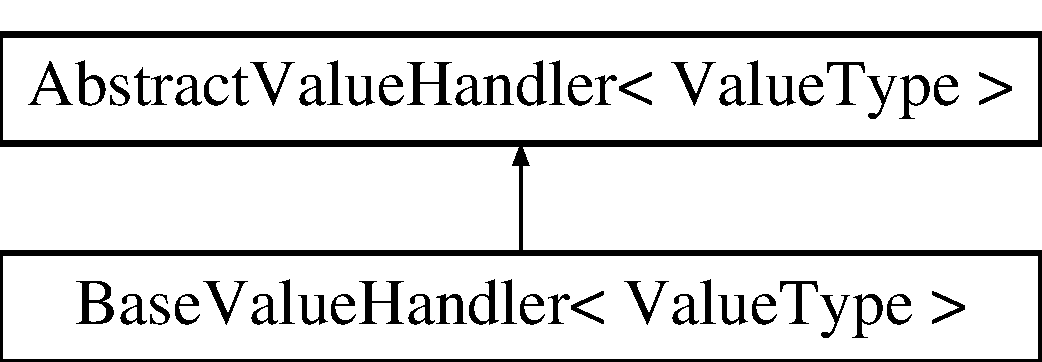
\includegraphics[height=2.000000cm]{classAbstractValueHandler}
\end{center}
\end{figure}
\subsection*{Public Member Functions}
\begin{DoxyCompactItemize}
\item 
virtual std\+::string \hyperlink{classAbstractValueHandler_a6e2f7abe130cdec1062e51d56e4f9fac}{id} ()
\item 
virtual void \hyperlink{classAbstractValueHandler_ac7921fae157361b054e467bf96785654}{read} (std\+::istream $\ast$in, Value\+Type \&value)=0
\item 
virtual void \hyperlink{classAbstractValueHandler_aecd2820bc132f8065babbec5cd7458b8}{write} (std\+::ostream $\ast$out, Value\+Type \&value)=0
\item 
virtual std\+::string \hyperlink{classAbstractValueHandler_a8e56e3bbccc464a47a666352249e6a1b}{tostring} (Value\+Type \&value)=0
\item 
virtual unsigned int \hyperlink{classAbstractValueHandler_a1d5941f6ff2afaee0c0bfc89ccb5188e}{count} (Value\+Type \&value) const  =0
\item 
virtual void \hyperlink{classAbstractValueHandler_a72ecec2580cb5a9a3ba1495a98d08d98}{add} (Value\+Type $\ast$value, const \hyperlink{classIndexReference}{Index\+Reference} \&ref) const  =0
\item 
virtual void \hyperlink{classAbstractValueHandler_ae89579ec77805153a0acc617202f89b4}{convertto} (Value\+Type $\ast$source, Value\+Type $\ast$\&target) const 
\end{DoxyCompactItemize}


\subsection{Detailed Description}
\subsubsection*{template$<$class Value\+Type$>$class Abstract\+Value\+Handler$<$ Value\+Type $>$}

Abstract value handler class, all value handlers are derived from this. Value handlers are interfaces to the values in \hyperlink{classPattern}{Pattern} Maps. They are used to abstract from the actual value data type and provide some common methods required for all values, as well at methods for serialisation from/to binary file. All are derived from the abstract class \hyperlink{classAbstractValueHandler}{Abstract\+Value\+Handler}. 

\subsection{Member Function Documentation}
\hypertarget{classAbstractValueHandler_a72ecec2580cb5a9a3ba1495a98d08d98}{}\index{Abstract\+Value\+Handler@{Abstract\+Value\+Handler}!add@{add}}
\index{add@{add}!Abstract\+Value\+Handler@{Abstract\+Value\+Handler}}
\subsubsection[{add(\+Value\+Type $\ast$value, const Index\+Reference \&ref) const  =0}]{\setlength{\rightskip}{0pt plus 5cm}template$<$class Value\+Type$>$ virtual void {\bf Abstract\+Value\+Handler}$<$ Value\+Type $>$\+::add (
\begin{DoxyParamCaption}
\item[{Value\+Type $\ast$}]{value, }
\item[{const {\bf Index\+Reference} \&}]{ref}
\end{DoxyParamCaption}
) const\hspace{0.3cm}{\ttfamily [pure virtual]}}\label{classAbstractValueHandler_a72ecec2580cb5a9a3ba1495a98d08d98}


Implemented in \hyperlink{classPatternStoreValueHandler_af05f8053a126fa4a0b100a2a70258977}{Pattern\+Store\+Value\+Handler$<$ Pattern\+Store\+Type $>$}, \hyperlink{classPatternStoreValueHandler_af05f8053a126fa4a0b100a2a70258977}{Pattern\+Store\+Value\+Handler$<$ Pattern\+Map$<$ Value\+Type, Value\+Handler, Nested\+Size\+Type $>$ $>$}, \hyperlink{classPatternFeatureVectorMapHandler_ab234259fb46c86986d41b0ef81a3b0c0}{Pattern\+Feature\+Vector\+Map\+Handler$<$ Feature\+Type $>$}, \hyperlink{classIndexedDataHandler_a242beac1d0b430238e3259556d2b1426}{Indexed\+Data\+Handler}, and \hyperlink{classBaseValueHandler_a260db19187a4f3fdd6dcf1fed7ac6a59}{Base\+Value\+Handler$<$ Value\+Type $>$}.

\hypertarget{classAbstractValueHandler_ae89579ec77805153a0acc617202f89b4}{}\index{Abstract\+Value\+Handler@{Abstract\+Value\+Handler}!convertto@{convertto}}
\index{convertto@{convertto}!Abstract\+Value\+Handler@{Abstract\+Value\+Handler}}
\subsubsection[{convertto(\+Value\+Type $\ast$source, Value\+Type $\ast$\&target) const }]{\setlength{\rightskip}{0pt plus 5cm}template$<$class Value\+Type$>$ virtual void {\bf Abstract\+Value\+Handler}$<$ Value\+Type $>$\+::convertto (
\begin{DoxyParamCaption}
\item[{Value\+Type $\ast$}]{source, }
\item[{Value\+Type $\ast$\&}]{target}
\end{DoxyParamCaption}
) const\hspace{0.3cm}{\ttfamily [inline]}, {\ttfamily [virtual]}}\label{classAbstractValueHandler_ae89579ec77805153a0acc617202f89b4}


Reimplemented in \hyperlink{classPatternFeatureVectorMapHandler_ad69265b8885d3fba7e557a39c3632768}{Pattern\+Feature\+Vector\+Map\+Handler$<$ Feature\+Type $>$}, \hyperlink{classIndexedDataHandler_a5f4e87e6b1d952f9a1724168786bc99e}{Indexed\+Data\+Handler}, and \hyperlink{classBaseValueHandler_a6b00505c99c8ba21309d8306e423a109}{Base\+Value\+Handler$<$ Value\+Type $>$}.

\hypertarget{classAbstractValueHandler_a1d5941f6ff2afaee0c0bfc89ccb5188e}{}\index{Abstract\+Value\+Handler@{Abstract\+Value\+Handler}!count@{count}}
\index{count@{count}!Abstract\+Value\+Handler@{Abstract\+Value\+Handler}}
\subsubsection[{count(\+Value\+Type \&value) const  =0}]{\setlength{\rightskip}{0pt plus 5cm}template$<$class Value\+Type$>$ virtual unsigned int {\bf Abstract\+Value\+Handler}$<$ Value\+Type $>$\+::count (
\begin{DoxyParamCaption}
\item[{Value\+Type \&}]{value}
\end{DoxyParamCaption}
) const\hspace{0.3cm}{\ttfamily [pure virtual]}}\label{classAbstractValueHandler_a1d5941f6ff2afaee0c0bfc89ccb5188e}


Implemented in \hyperlink{classPatternStoreValueHandler_af967671eda3e9ab05c0bf05ca9d0dfae}{Pattern\+Store\+Value\+Handler$<$ Pattern\+Store\+Type $>$}, \hyperlink{classPatternStoreValueHandler_af967671eda3e9ab05c0bf05ca9d0dfae}{Pattern\+Store\+Value\+Handler$<$ Pattern\+Map$<$ Value\+Type, Value\+Handler, Nested\+Size\+Type $>$ $>$}, \hyperlink{classPatternFeatureVectorMapHandler_a67a49821f7c2b8b4d6e1e5be81c36bd4}{Pattern\+Feature\+Vector\+Map\+Handler$<$ Feature\+Type $>$}, \hyperlink{classIndexedDataHandler_a9ce91a864dceb5e7de23ee89d1083037}{Indexed\+Data\+Handler}, and \hyperlink{classBaseValueHandler_a841fab906106fcfdef995e7b9c594ef4}{Base\+Value\+Handler$<$ Value\+Type $>$}.

\hypertarget{classAbstractValueHandler_a6e2f7abe130cdec1062e51d56e4f9fac}{}\index{Abstract\+Value\+Handler@{Abstract\+Value\+Handler}!id@{id}}
\index{id@{id}!Abstract\+Value\+Handler@{Abstract\+Value\+Handler}}
\subsubsection[{id()}]{\setlength{\rightskip}{0pt plus 5cm}template$<$class Value\+Type$>$ virtual std\+::string {\bf Abstract\+Value\+Handler}$<$ Value\+Type $>$\+::id (
\begin{DoxyParamCaption}
{}
\end{DoxyParamCaption}
)\hspace{0.3cm}{\ttfamily [inline]}, {\ttfamily [virtual]}}\label{classAbstractValueHandler_a6e2f7abe130cdec1062e51d56e4f9fac}


Reimplemented in \hyperlink{classPatternStoreValueHandler_a8f1745d36fe84bd8b96854a30b3bc5f7}{Pattern\+Store\+Value\+Handler$<$ Pattern\+Store\+Type $>$}, \hyperlink{classPatternStoreValueHandler_a8f1745d36fe84bd8b96854a30b3bc5f7}{Pattern\+Store\+Value\+Handler$<$ Pattern\+Map$<$ Value\+Type, Value\+Handler, Nested\+Size\+Type $>$ $>$}, \hyperlink{classArrayValueHandler_ac82e2a0341b8f0e66b36a07b91fbed42}{Array\+Value\+Handler$<$ T, N, countindex $>$}, \hyperlink{classPatternFeatureVectorMapHandler_ac3a86c293fbc3417ae6d8dc13389be82}{Pattern\+Feature\+Vector\+Map\+Handler$<$ Feature\+Type $>$}, \hyperlink{classIndexedDataHandler_a858b6661224371858487adf4515a929c}{Indexed\+Data\+Handler}, and \hyperlink{classBaseValueHandler_a7bc1637a355d28baa52bc3f1e069bfb7}{Base\+Value\+Handler$<$ Value\+Type $>$}.

\hypertarget{classAbstractValueHandler_ac7921fae157361b054e467bf96785654}{}\index{Abstract\+Value\+Handler@{Abstract\+Value\+Handler}!read@{read}}
\index{read@{read}!Abstract\+Value\+Handler@{Abstract\+Value\+Handler}}
\subsubsection[{read(std\+::istream $\ast$in, Value\+Type \&value)=0}]{\setlength{\rightskip}{0pt plus 5cm}template$<$class Value\+Type$>$ virtual void {\bf Abstract\+Value\+Handler}$<$ Value\+Type $>$\+::read (
\begin{DoxyParamCaption}
\item[{std\+::istream $\ast$}]{in, }
\item[{Value\+Type \&}]{value}
\end{DoxyParamCaption}
)\hspace{0.3cm}{\ttfamily [pure virtual]}}\label{classAbstractValueHandler_ac7921fae157361b054e467bf96785654}


Implemented in \hyperlink{classPatternStoreValueHandler_a1ee31fd587f60c2c10200581724fbee6}{Pattern\+Store\+Value\+Handler$<$ Pattern\+Store\+Type $>$}, \hyperlink{classPatternStoreValueHandler_a1ee31fd587f60c2c10200581724fbee6}{Pattern\+Store\+Value\+Handler$<$ Pattern\+Map$<$ Value\+Type, Value\+Handler, Nested\+Size\+Type $>$ $>$}, \hyperlink{classPatternFeatureVectorMapHandler_a3956b0d0deccf1a3f36135d084a30627}{Pattern\+Feature\+Vector\+Map\+Handler$<$ Feature\+Type $>$}, \hyperlink{classIndexedDataHandler_ab24da9862e5572a9d6f58e51f62fb5c7}{Indexed\+Data\+Handler}, and \hyperlink{classBaseValueHandler_ae55dd264dd8dcd4e9105a36fa8211df8}{Base\+Value\+Handler$<$ Value\+Type $>$}.

\hypertarget{classAbstractValueHandler_a8e56e3bbccc464a47a666352249e6a1b}{}\index{Abstract\+Value\+Handler@{Abstract\+Value\+Handler}!tostring@{tostring}}
\index{tostring@{tostring}!Abstract\+Value\+Handler@{Abstract\+Value\+Handler}}
\subsubsection[{tostring(\+Value\+Type \&value)=0}]{\setlength{\rightskip}{0pt plus 5cm}template$<$class Value\+Type$>$ virtual std\+::string {\bf Abstract\+Value\+Handler}$<$ Value\+Type $>$\+::tostring (
\begin{DoxyParamCaption}
\item[{Value\+Type \&}]{value}
\end{DoxyParamCaption}
)\hspace{0.3cm}{\ttfamily [pure virtual]}}\label{classAbstractValueHandler_a8e56e3bbccc464a47a666352249e6a1b}


Implemented in \hyperlink{classPatternStoreValueHandler_ac976813f02dcad60eb8cb700c6ba0753}{Pattern\+Store\+Value\+Handler$<$ Pattern\+Store\+Type $>$}, \hyperlink{classPatternStoreValueHandler_ac976813f02dcad60eb8cb700c6ba0753}{Pattern\+Store\+Value\+Handler$<$ Pattern\+Map$<$ Value\+Type, Value\+Handler, Nested\+Size\+Type $>$ $>$}, \hyperlink{classPatternFeatureVectorMapHandler_a27faed3107244e4ab0f53e3acea201de}{Pattern\+Feature\+Vector\+Map\+Handler$<$ Feature\+Type $>$}, \hyperlink{classIndexedDataHandler_a7a3fd16bf83956b3fbc2fe46578aa958}{Indexed\+Data\+Handler}, and \hyperlink{classBaseValueHandler_a486eb004615965908cf2a5e670d55293}{Base\+Value\+Handler$<$ Value\+Type $>$}.

\hypertarget{classAbstractValueHandler_aecd2820bc132f8065babbec5cd7458b8}{}\index{Abstract\+Value\+Handler@{Abstract\+Value\+Handler}!write@{write}}
\index{write@{write}!Abstract\+Value\+Handler@{Abstract\+Value\+Handler}}
\subsubsection[{write(std\+::ostream $\ast$out, Value\+Type \&value)=0}]{\setlength{\rightskip}{0pt plus 5cm}template$<$class Value\+Type$>$ virtual void {\bf Abstract\+Value\+Handler}$<$ Value\+Type $>$\+::write (
\begin{DoxyParamCaption}
\item[{std\+::ostream $\ast$}]{out, }
\item[{Value\+Type \&}]{value}
\end{DoxyParamCaption}
)\hspace{0.3cm}{\ttfamily [pure virtual]}}\label{classAbstractValueHandler_aecd2820bc132f8065babbec5cd7458b8}


Implemented in \hyperlink{classPatternStoreValueHandler_a64d152c70a8ffd4f5ffdb09abb570b2d}{Pattern\+Store\+Value\+Handler$<$ Pattern\+Store\+Type $>$}, \hyperlink{classPatternStoreValueHandler_a64d152c70a8ffd4f5ffdb09abb570b2d}{Pattern\+Store\+Value\+Handler$<$ Pattern\+Map$<$ Value\+Type, Value\+Handler, Nested\+Size\+Type $>$ $>$}, \hyperlink{classPatternFeatureVectorMapHandler_a188df59b0fe05271e3ee90ba20204ffa}{Pattern\+Feature\+Vector\+Map\+Handler$<$ Feature\+Type $>$}, \hyperlink{classIndexedDataHandler_adac292491ac7e7e59d15f0a8a76bfac7}{Indexed\+Data\+Handler}, and \hyperlink{classBaseValueHandler_a56854e807c698507ddfeab331abd0482}{Base\+Value\+Handler$<$ Value\+Type $>$}.



The documentation for this class was generated from the following file\+:\begin{DoxyCompactItemize}
\item 
include/\hyperlink{datatypes_8h}{datatypes.\+h}\end{DoxyCompactItemize}

\hypertarget{classAlignedPatternMap}{}\section{Aligned\+Pattern\+Map$<$ Value\+Type, Value\+Handler, Nested\+Size\+Type $>$ Class Template Reference}
\label{classAlignedPatternMap}\index{Aligned\+Pattern\+Map$<$ Value\+Type, Value\+Handler, Nested\+Size\+Type $>$@{Aligned\+Pattern\+Map$<$ Value\+Type, Value\+Handler, Nested\+Size\+Type $>$}}


A nested pattern map, useful for storing patterns that map to other patterns, which in turn map to values. An example is phrase-\/translation tables in Machine Translation.  




{\ttfamily \#include $<$patternstore.\+h$>$}

Inheritance diagram for Aligned\+Pattern\+Map$<$ Value\+Type, Value\+Handler, Nested\+Size\+Type $>$\+:\begin{figure}[H]
\begin{center}
\leavevmode
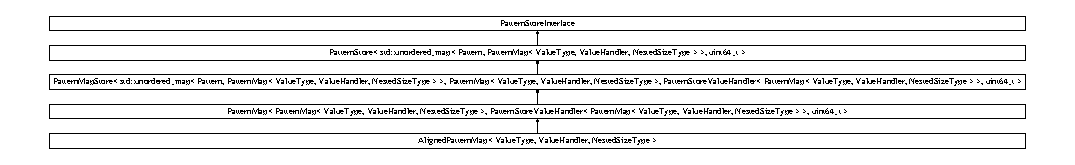
\includegraphics[height=1.775523cm]{classAlignedPatternMap}
\end{center}
\end{figure}
\subsection*{Public Types}
\begin{DoxyCompactItemize}
\item 
typedef \hyperlink{classPatternMap}{Pattern\+Map}$<$ Value\+Type, Value\+Handler, Nested\+Size\+Type $>$ \hyperlink{classAlignedPatternMap_a5b139dad8d98612f62fc561a1e29153d}{valuetype}
\item 
typedef \hyperlink{classPatternMap}{Pattern\+Map}$<$ \hyperlink{classPatternMap}{Pattern\+Map}$<$ Value\+Type, Value\+Handler, Nested\+Size\+Type $>$, \hyperlink{classPatternStoreValueHandler}{Pattern\+Store\+Value\+Handler}$<$ \hyperlink{classPatternMap}{Pattern\+Map}$<$ Value\+Type, Value\+Handler, Nested\+Size\+Type $>$ $>$, uint64\+\_\+t $>$\+::\hyperlink{classAlignedPatternMap_ac784198ebf47e631d2feb1c9d6063b1b}{iterator} \hyperlink{classAlignedPatternMap_ac784198ebf47e631d2feb1c9d6063b1b}{iterator}
\item 
typedef \hyperlink{classPatternMap}{Pattern\+Map}$<$ \hyperlink{classPatternMap}{Pattern\+Map}$<$ Value\+Type, Value\+Handler, Nested\+Size\+Type $>$, \hyperlink{classPatternStoreValueHandler}{Pattern\+Store\+Value\+Handler}$<$ \hyperlink{classPatternMap}{Pattern\+Map}$<$ Value\+Type, Value\+Handler, Nested\+Size\+Type $>$ $>$, uint64\+\_\+t $>$\+::\hyperlink{classAlignedPatternMap_a1dd59a53ad5586979698949f2845a1ee}{const\+\_\+iterator} \hyperlink{classAlignedPatternMap_a1dd59a53ad5586979698949f2845a1ee}{const\+\_\+iterator}
\end{DoxyCompactItemize}
\subsection*{Additional Inherited Members}


\subsection{Detailed Description}
\subsubsection*{template$<$class Value\+Type, class Value\+Handler = Base\+Value\+Handler$<$\+Value\+Type$>$, class Nested\+Size\+Type = uint16\+\_\+t$>$class Aligned\+Pattern\+Map$<$ Value\+Type, Value\+Handler, Nested\+Size\+Type $>$}

A nested pattern map, useful for storing patterns that map to other patterns, which in turn map to values. An example is phrase-\/translation tables in Machine Translation. 

\subsection{Member Typedef Documentation}
\hypertarget{classAlignedPatternMap_a1dd59a53ad5586979698949f2845a1ee}{}\index{Aligned\+Pattern\+Map@{Aligned\+Pattern\+Map}!const\+\_\+iterator@{const\+\_\+iterator}}
\index{const\+\_\+iterator@{const\+\_\+iterator}!Aligned\+Pattern\+Map@{Aligned\+Pattern\+Map}}
\subsubsection[{const\+\_\+iterator}]{\setlength{\rightskip}{0pt plus 5cm}template$<$class Value\+Type , class Value\+Handler  = Base\+Value\+Handler$<$\+Value\+Type$>$, class Nested\+Size\+Type  = uint16\+\_\+t$>$ typedef {\bf Pattern\+Map}$<$ {\bf Pattern\+Map}$<$Value\+Type,Value\+Handler,Nested\+Size\+Type$>$,{\bf Pattern\+Store\+Value\+Handler}$<${\bf Pattern\+Map}$<$Value\+Type,Value\+Handler,Nested\+Size\+Type$>$ $>$, uint64\+\_\+t $>$\+::{\bf const\+\_\+iterator} {\bf Aligned\+Pattern\+Map}$<$ Value\+Type, Value\+Handler, Nested\+Size\+Type $>$\+::{\bf const\+\_\+iterator}}\label{classAlignedPatternMap_a1dd59a53ad5586979698949f2845a1ee}
\hypertarget{classAlignedPatternMap_ac784198ebf47e631d2feb1c9d6063b1b}{}\index{Aligned\+Pattern\+Map@{Aligned\+Pattern\+Map}!iterator@{iterator}}
\index{iterator@{iterator}!Aligned\+Pattern\+Map@{Aligned\+Pattern\+Map}}
\subsubsection[{iterator}]{\setlength{\rightskip}{0pt plus 5cm}template$<$class Value\+Type , class Value\+Handler  = Base\+Value\+Handler$<$\+Value\+Type$>$, class Nested\+Size\+Type  = uint16\+\_\+t$>$ typedef {\bf Pattern\+Map}$<$ {\bf Pattern\+Map}$<$Value\+Type,Value\+Handler,Nested\+Size\+Type$>$,{\bf Pattern\+Store\+Value\+Handler}$<${\bf Pattern\+Map}$<$Value\+Type,Value\+Handler,Nested\+Size\+Type$>$ $>$, uint64\+\_\+t $>$\+::{\bf iterator} {\bf Aligned\+Pattern\+Map}$<$ Value\+Type, Value\+Handler, Nested\+Size\+Type $>$\+::{\bf iterator}}\label{classAlignedPatternMap_ac784198ebf47e631d2feb1c9d6063b1b}
\hypertarget{classAlignedPatternMap_a5b139dad8d98612f62fc561a1e29153d}{}\index{Aligned\+Pattern\+Map@{Aligned\+Pattern\+Map}!valuetype@{valuetype}}
\index{valuetype@{valuetype}!Aligned\+Pattern\+Map@{Aligned\+Pattern\+Map}}
\subsubsection[{valuetype}]{\setlength{\rightskip}{0pt plus 5cm}template$<$class Value\+Type , class Value\+Handler  = Base\+Value\+Handler$<$\+Value\+Type$>$, class Nested\+Size\+Type  = uint16\+\_\+t$>$ typedef {\bf Pattern\+Map}$<$Value\+Type,Value\+Handler,Nested\+Size\+Type$>$ {\bf Aligned\+Pattern\+Map}$<$ Value\+Type, Value\+Handler, Nested\+Size\+Type $>$\+::{\bf valuetype}}\label{classAlignedPatternMap_a5b139dad8d98612f62fc561a1e29153d}


The documentation for this class was generated from the following file\+:\begin{DoxyCompactItemize}
\item 
include/\hyperlink{patternstore_8h}{patternstore.\+h}\end{DoxyCompactItemize}

\hypertarget{classArrayValueHandler}{}\section{Array\+Value\+Handler$<$ T, N, countindex $>$ Class Template Reference}
\label{classArrayValueHandler}\index{Array\+Value\+Handler$<$ T, N, countindex $>$@{Array\+Value\+Handler$<$ T, N, countindex $>$}}


{\ttfamily \#include $<$patternstore.\+h$>$}

Inheritance diagram for Array\+Value\+Handler$<$ T, N, countindex $>$\+:\begin{figure}[H]
\begin{center}
\leavevmode
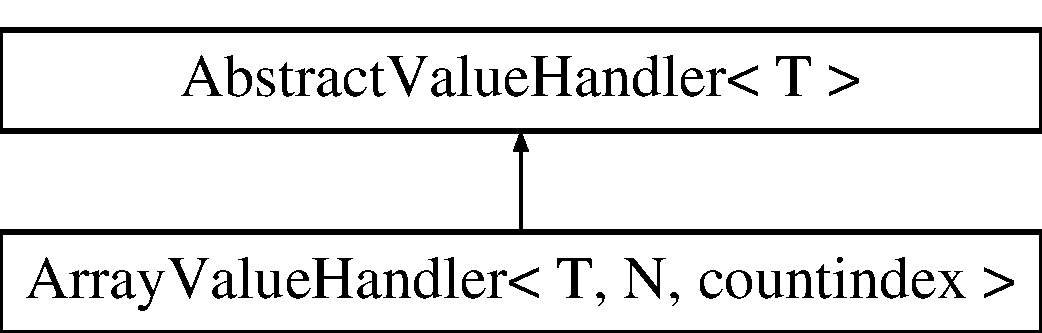
\includegraphics[height=2.000000cm]{classArrayValueHandler}
\end{center}
\end{figure}
\subsection*{Public Member Functions}
\begin{DoxyCompactItemize}
\item 
virtual std\+::string \hyperlink{classArrayValueHandler_ac82e2a0341b8f0e66b36a07b91fbed42}{id} ()
\item 
void \hyperlink{classArrayValueHandler_a35c445a9b0de620ca4b032e0a34d0dee}{read} (std\+::istream $\ast$in, std\+::array$<$ T, N $>$ \&a)
\item 
void \hyperlink{classArrayValueHandler_ab081c8ac7e02d523bb8198611c90284c}{write} (std\+::ostream $\ast$out, std\+::array$<$ T, N $>$ \&a)
\item 
std\+::string \hyperlink{classArrayValueHandler_a51b18a3051bc51765731601edbdc8e34}{tostring} (std\+::array$<$ T, N $>$ \&a)
\item 
unsigned int \hyperlink{classArrayValueHandler_aa0b5815b513c2886172d0a028ffb2ff3}{count} (std\+::array$<$ T, N $>$ \&a) const 
\item 
void \hyperlink{classArrayValueHandler_a11702281d720f428e59b38f25790b68e}{add} (std\+::array$<$ T, N $>$ $\ast$value, const \hyperlink{classIndexReference}{Index\+Reference} \&ref) const 
\end{DoxyCompactItemize}
\subsection*{Static Public Attributes}
\begin{DoxyCompactItemize}
\item 
static const bool \hyperlink{classArrayValueHandler_a89c7c6a8820236bc45f71f446400b851}{indexed} = false
\end{DoxyCompactItemize}


\subsection{Member Function Documentation}
\hypertarget{classArrayValueHandler_a11702281d720f428e59b38f25790b68e}{}\index{Array\+Value\+Handler@{Array\+Value\+Handler}!add@{add}}
\index{add@{add}!Array\+Value\+Handler@{Array\+Value\+Handler}}
\subsubsection[{add(std\+::array$<$ T, N $>$ $\ast$value, const Index\+Reference \&ref) const }]{\setlength{\rightskip}{0pt plus 5cm}template$<$class T , size\+\_\+t N, int countindex = 0$>$ void {\bf Array\+Value\+Handler}$<$ T, N, countindex $>$\+::add (
\begin{DoxyParamCaption}
\item[{std\+::array$<$ T, N $>$ $\ast$}]{value, }
\item[{const {\bf Index\+Reference} \&}]{ref}
\end{DoxyParamCaption}
) const\hspace{0.3cm}{\ttfamily [inline]}}\label{classArrayValueHandler_a11702281d720f428e59b38f25790b68e}
\hypertarget{classArrayValueHandler_aa0b5815b513c2886172d0a028ffb2ff3}{}\index{Array\+Value\+Handler@{Array\+Value\+Handler}!count@{count}}
\index{count@{count}!Array\+Value\+Handler@{Array\+Value\+Handler}}
\subsubsection[{count(std\+::array$<$ T, N $>$ \&a) const }]{\setlength{\rightskip}{0pt plus 5cm}template$<$class T , size\+\_\+t N, int countindex = 0$>$ unsigned int {\bf Array\+Value\+Handler}$<$ T, N, countindex $>$\+::count (
\begin{DoxyParamCaption}
\item[{std\+::array$<$ T, N $>$ \&}]{a}
\end{DoxyParamCaption}
) const\hspace{0.3cm}{\ttfamily [inline]}}\label{classArrayValueHandler_aa0b5815b513c2886172d0a028ffb2ff3}
\hypertarget{classArrayValueHandler_ac82e2a0341b8f0e66b36a07b91fbed42}{}\index{Array\+Value\+Handler@{Array\+Value\+Handler}!id@{id}}
\index{id@{id}!Array\+Value\+Handler@{Array\+Value\+Handler}}
\subsubsection[{id()}]{\setlength{\rightskip}{0pt plus 5cm}template$<$class T , size\+\_\+t N, int countindex = 0$>$ virtual std\+::string {\bf Array\+Value\+Handler}$<$ T, N, countindex $>$\+::id (
\begin{DoxyParamCaption}
{}
\end{DoxyParamCaption}
)\hspace{0.3cm}{\ttfamily [inline]}, {\ttfamily [virtual]}}\label{classArrayValueHandler_ac82e2a0341b8f0e66b36a07b91fbed42}


Reimplemented from \hyperlink{classAbstractValueHandler_a6e2f7abe130cdec1062e51d56e4f9fac}{Abstract\+Value\+Handler$<$ T $>$}.

\hypertarget{classArrayValueHandler_a35c445a9b0de620ca4b032e0a34d0dee}{}\index{Array\+Value\+Handler@{Array\+Value\+Handler}!read@{read}}
\index{read@{read}!Array\+Value\+Handler@{Array\+Value\+Handler}}
\subsubsection[{read(std\+::istream $\ast$in, std\+::array$<$ T, N $>$ \&a)}]{\setlength{\rightskip}{0pt plus 5cm}template$<$class T , size\+\_\+t N, int countindex = 0$>$ void {\bf Array\+Value\+Handler}$<$ T, N, countindex $>$\+::read (
\begin{DoxyParamCaption}
\item[{std\+::istream $\ast$}]{in, }
\item[{std\+::array$<$ T, N $>$ \&}]{a}
\end{DoxyParamCaption}
)\hspace{0.3cm}{\ttfamily [inline]}}\label{classArrayValueHandler_a35c445a9b0de620ca4b032e0a34d0dee}
\hypertarget{classArrayValueHandler_a51b18a3051bc51765731601edbdc8e34}{}\index{Array\+Value\+Handler@{Array\+Value\+Handler}!tostring@{tostring}}
\index{tostring@{tostring}!Array\+Value\+Handler@{Array\+Value\+Handler}}
\subsubsection[{tostring(std\+::array$<$ T, N $>$ \&a)}]{\setlength{\rightskip}{0pt plus 5cm}template$<$class T , size\+\_\+t N, int countindex = 0$>$ std\+::string {\bf Array\+Value\+Handler}$<$ T, N, countindex $>$\+::tostring (
\begin{DoxyParamCaption}
\item[{std\+::array$<$ T, N $>$ \&}]{a}
\end{DoxyParamCaption}
)\hspace{0.3cm}{\ttfamily [inline]}}\label{classArrayValueHandler_a51b18a3051bc51765731601edbdc8e34}
\hypertarget{classArrayValueHandler_ab081c8ac7e02d523bb8198611c90284c}{}\index{Array\+Value\+Handler@{Array\+Value\+Handler}!write@{write}}
\index{write@{write}!Array\+Value\+Handler@{Array\+Value\+Handler}}
\subsubsection[{write(std\+::ostream $\ast$out, std\+::array$<$ T, N $>$ \&a)}]{\setlength{\rightskip}{0pt plus 5cm}template$<$class T , size\+\_\+t N, int countindex = 0$>$ void {\bf Array\+Value\+Handler}$<$ T, N, countindex $>$\+::write (
\begin{DoxyParamCaption}
\item[{std\+::ostream $\ast$}]{out, }
\item[{std\+::array$<$ T, N $>$ \&}]{a}
\end{DoxyParamCaption}
)\hspace{0.3cm}{\ttfamily [inline]}}\label{classArrayValueHandler_ab081c8ac7e02d523bb8198611c90284c}


\subsection{Member Data Documentation}
\hypertarget{classArrayValueHandler_a89c7c6a8820236bc45f71f446400b851}{}\index{Array\+Value\+Handler@{Array\+Value\+Handler}!indexed@{indexed}}
\index{indexed@{indexed}!Array\+Value\+Handler@{Array\+Value\+Handler}}
\subsubsection[{indexed}]{\setlength{\rightskip}{0pt plus 5cm}template$<$class T , size\+\_\+t N, int countindex = 0$>$ const bool {\bf Array\+Value\+Handler}$<$ T, N, countindex $>$\+::indexed = false\hspace{0.3cm}{\ttfamily [static]}}\label{classArrayValueHandler_a89c7c6a8820236bc45f71f446400b851}


The documentation for this class was generated from the following file\+:\begin{DoxyCompactItemize}
\item 
include/\hyperlink{patternstore_8h}{patternstore.\+h}\end{DoxyCompactItemize}

\hypertarget{classBaseValueHandler}{}\section{Base\+Value\+Handler$<$ Value\+Type $>$ Class Template Reference}
\label{classBaseValueHandler}\index{Base\+Value\+Handler$<$ Value\+Type $>$@{Base\+Value\+Handler$<$ Value\+Type $>$}}


This templated class can be used for all numeric base types (such as int, uint16\+\_\+t, float, etc).  




{\ttfamily \#include $<$datatypes.\+h$>$}

Inheritance diagram for Base\+Value\+Handler$<$ Value\+Type $>$\+:\begin{figure}[H]
\begin{center}
\leavevmode
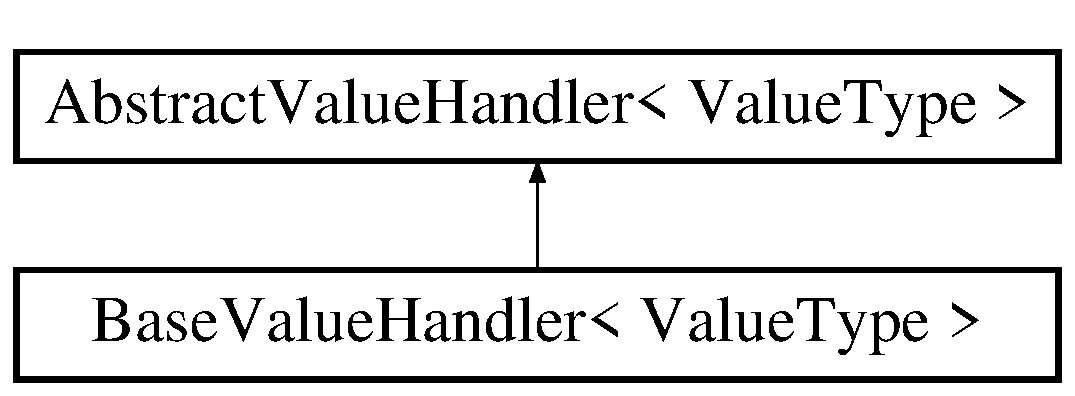
\includegraphics[height=2.000000cm]{classBaseValueHandler}
\end{center}
\end{figure}
\subsection*{Public Member Functions}
\begin{DoxyCompactItemize}
\item 
virtual std\+::string \hyperlink{classBaseValueHandler_a7bc1637a355d28baa52bc3f1e069bfb7}{id} ()
\item 
void \hyperlink{classBaseValueHandler_ae55dd264dd8dcd4e9105a36fa8211df8}{read} (std\+::istream $\ast$in, Value\+Type \&v)
\item 
void \hyperlink{classBaseValueHandler_a56854e807c698507ddfeab331abd0482}{write} (std\+::ostream $\ast$out, Value\+Type \&value)
\item 
virtual std\+::string \hyperlink{classBaseValueHandler_a486eb004615965908cf2a5e670d55293}{tostring} (Value\+Type \&value)
\item 
unsigned int \hyperlink{classBaseValueHandler_a841fab906106fcfdef995e7b9c594ef4}{count} (Value\+Type \&value) const 
\item 
void \hyperlink{classBaseValueHandler_a260db19187a4f3fdd6dcf1fed7ac6a59}{add} (Value\+Type $\ast$value, const \hyperlink{classIndexReference}{Index\+Reference} \&ref) const 
\item 
void \hyperlink{classBaseValueHandler_a6b00505c99c8ba21309d8306e423a109}{convertto} (Value\+Type $\ast$source, Value\+Type $\ast$\&target) const 
\item 
void \hyperlink{classBaseValueHandler_aeb47f3d86de265e9c1ef5f4af39f941b}{convertto} (Value\+Type $\ast$source, \hyperlink{classIndexedData}{Indexed\+Data} $\ast$\&target) const 
\end{DoxyCompactItemize}
\subsection*{Static Public Attributes}
\begin{DoxyCompactItemize}
\item 
static const bool \hyperlink{classBaseValueHandler_a53a7fc222b1aa001cedacec165c58203}{indexed} = false
\end{DoxyCompactItemize}


\subsection{Detailed Description}
\subsubsection*{template$<$class Value\+Type$>$class Base\+Value\+Handler$<$ Value\+Type $>$}

This templated class can be used for all numeric base types (such as int, uint16\+\_\+t, float, etc). 


\begin{DoxyTemplParams}{Template Parameters}
{\em Value\+Type} & the actual numeric base type used \\
\hline
\end{DoxyTemplParams}


\subsection{Member Function Documentation}
\hypertarget{classBaseValueHandler_a260db19187a4f3fdd6dcf1fed7ac6a59}{}\index{Base\+Value\+Handler@{Base\+Value\+Handler}!add@{add}}
\index{add@{add}!Base\+Value\+Handler@{Base\+Value\+Handler}}
\subsubsection[{add(\+Value\+Type $\ast$value, const Index\+Reference \&ref) const }]{\setlength{\rightskip}{0pt plus 5cm}template$<$class Value\+Type $>$ void {\bf Base\+Value\+Handler}$<$ Value\+Type $>$\+::add (
\begin{DoxyParamCaption}
\item[{Value\+Type $\ast$}]{value, }
\item[{const {\bf Index\+Reference} \&}]{ref}
\end{DoxyParamCaption}
) const\hspace{0.3cm}{\ttfamily [inline]}, {\ttfamily [virtual]}}\label{classBaseValueHandler_a260db19187a4f3fdd6dcf1fed7ac6a59}


Implements \hyperlink{classAbstractValueHandler_a72ecec2580cb5a9a3ba1495a98d08d98}{Abstract\+Value\+Handler$<$ Value\+Type $>$}.

\hypertarget{classBaseValueHandler_a6b00505c99c8ba21309d8306e423a109}{}\index{Base\+Value\+Handler@{Base\+Value\+Handler}!convertto@{convertto}}
\index{convertto@{convertto}!Base\+Value\+Handler@{Base\+Value\+Handler}}
\subsubsection[{convertto(\+Value\+Type $\ast$source, Value\+Type $\ast$\&target) const }]{\setlength{\rightskip}{0pt plus 5cm}template$<$class Value\+Type $>$ void {\bf Base\+Value\+Handler}$<$ Value\+Type $>$\+::convertto (
\begin{DoxyParamCaption}
\item[{Value\+Type $\ast$}]{source, }
\item[{Value\+Type $\ast$\&}]{target}
\end{DoxyParamCaption}
) const\hspace{0.3cm}{\ttfamily [inline]}, {\ttfamily [virtual]}}\label{classBaseValueHandler_a6b00505c99c8ba21309d8306e423a109}


Reimplemented from \hyperlink{classAbstractValueHandler_ae89579ec77805153a0acc617202f89b4}{Abstract\+Value\+Handler$<$ Value\+Type $>$}.

\hypertarget{classBaseValueHandler_aeb47f3d86de265e9c1ef5f4af39f941b}{}\index{Base\+Value\+Handler@{Base\+Value\+Handler}!convertto@{convertto}}
\index{convertto@{convertto}!Base\+Value\+Handler@{Base\+Value\+Handler}}
\subsubsection[{convertto(\+Value\+Type $\ast$source, Indexed\+Data $\ast$\&target) const }]{\setlength{\rightskip}{0pt plus 5cm}template$<$class Value\+Type $>$ void {\bf Base\+Value\+Handler}$<$ Value\+Type $>$\+::convertto (
\begin{DoxyParamCaption}
\item[{Value\+Type $\ast$}]{source, }
\item[{{\bf Indexed\+Data} $\ast$\&}]{target}
\end{DoxyParamCaption}
) const\hspace{0.3cm}{\ttfamily [inline]}}\label{classBaseValueHandler_aeb47f3d86de265e9c1ef5f4af39f941b}
\hypertarget{classBaseValueHandler_a841fab906106fcfdef995e7b9c594ef4}{}\index{Base\+Value\+Handler@{Base\+Value\+Handler}!count@{count}}
\index{count@{count}!Base\+Value\+Handler@{Base\+Value\+Handler}}
\subsubsection[{count(\+Value\+Type \&value) const }]{\setlength{\rightskip}{0pt plus 5cm}template$<$class Value\+Type $>$ unsigned int {\bf Base\+Value\+Handler}$<$ Value\+Type $>$\+::count (
\begin{DoxyParamCaption}
\item[{Value\+Type \&}]{value}
\end{DoxyParamCaption}
) const\hspace{0.3cm}{\ttfamily [inline]}, {\ttfamily [virtual]}}\label{classBaseValueHandler_a841fab906106fcfdef995e7b9c594ef4}


Implements \hyperlink{classAbstractValueHandler_a1d5941f6ff2afaee0c0bfc89ccb5188e}{Abstract\+Value\+Handler$<$ Value\+Type $>$}.

\hypertarget{classBaseValueHandler_a7bc1637a355d28baa52bc3f1e069bfb7}{}\index{Base\+Value\+Handler@{Base\+Value\+Handler}!id@{id}}
\index{id@{id}!Base\+Value\+Handler@{Base\+Value\+Handler}}
\subsubsection[{id()}]{\setlength{\rightskip}{0pt plus 5cm}template$<$class Value\+Type $>$ virtual std\+::string {\bf Base\+Value\+Handler}$<$ Value\+Type $>$\+::id (
\begin{DoxyParamCaption}
{}
\end{DoxyParamCaption}
)\hspace{0.3cm}{\ttfamily [inline]}, {\ttfamily [virtual]}}\label{classBaseValueHandler_a7bc1637a355d28baa52bc3f1e069bfb7}


Reimplemented from \hyperlink{classAbstractValueHandler_a6e2f7abe130cdec1062e51d56e4f9fac}{Abstract\+Value\+Handler$<$ Value\+Type $>$}.

\hypertarget{classBaseValueHandler_ae55dd264dd8dcd4e9105a36fa8211df8}{}\index{Base\+Value\+Handler@{Base\+Value\+Handler}!read@{read}}
\index{read@{read}!Base\+Value\+Handler@{Base\+Value\+Handler}}
\subsubsection[{read(std\+::istream $\ast$in, Value\+Type \&v)}]{\setlength{\rightskip}{0pt plus 5cm}template$<$class Value\+Type $>$ void {\bf Base\+Value\+Handler}$<$ Value\+Type $>$\+::read (
\begin{DoxyParamCaption}
\item[{std\+::istream $\ast$}]{in, }
\item[{Value\+Type \&}]{v}
\end{DoxyParamCaption}
)\hspace{0.3cm}{\ttfamily [inline]}, {\ttfamily [virtual]}}\label{classBaseValueHandler_ae55dd264dd8dcd4e9105a36fa8211df8}


Implements \hyperlink{classAbstractValueHandler_ac7921fae157361b054e467bf96785654}{Abstract\+Value\+Handler$<$ Value\+Type $>$}.

\hypertarget{classBaseValueHandler_a486eb004615965908cf2a5e670d55293}{}\index{Base\+Value\+Handler@{Base\+Value\+Handler}!tostring@{tostring}}
\index{tostring@{tostring}!Base\+Value\+Handler@{Base\+Value\+Handler}}
\subsubsection[{tostring(\+Value\+Type \&value)}]{\setlength{\rightskip}{0pt plus 5cm}template$<$class Value\+Type $>$ virtual std\+::string {\bf Base\+Value\+Handler}$<$ Value\+Type $>$\+::tostring (
\begin{DoxyParamCaption}
\item[{Value\+Type \&}]{value}
\end{DoxyParamCaption}
)\hspace{0.3cm}{\ttfamily [inline]}, {\ttfamily [virtual]}}\label{classBaseValueHandler_a486eb004615965908cf2a5e670d55293}


Implements \hyperlink{classAbstractValueHandler_a8e56e3bbccc464a47a666352249e6a1b}{Abstract\+Value\+Handler$<$ Value\+Type $>$}.

\hypertarget{classBaseValueHandler_a56854e807c698507ddfeab331abd0482}{}\index{Base\+Value\+Handler@{Base\+Value\+Handler}!write@{write}}
\index{write@{write}!Base\+Value\+Handler@{Base\+Value\+Handler}}
\subsubsection[{write(std\+::ostream $\ast$out, Value\+Type \&value)}]{\setlength{\rightskip}{0pt plus 5cm}template$<$class Value\+Type $>$ void {\bf Base\+Value\+Handler}$<$ Value\+Type $>$\+::write (
\begin{DoxyParamCaption}
\item[{std\+::ostream $\ast$}]{out, }
\item[{Value\+Type \&}]{value}
\end{DoxyParamCaption}
)\hspace{0.3cm}{\ttfamily [inline]}, {\ttfamily [virtual]}}\label{classBaseValueHandler_a56854e807c698507ddfeab331abd0482}


Implements \hyperlink{classAbstractValueHandler_aecd2820bc132f8065babbec5cd7458b8}{Abstract\+Value\+Handler$<$ Value\+Type $>$}.



\subsection{Member Data Documentation}
\hypertarget{classBaseValueHandler_a53a7fc222b1aa001cedacec165c58203}{}\index{Base\+Value\+Handler@{Base\+Value\+Handler}!indexed@{indexed}}
\index{indexed@{indexed}!Base\+Value\+Handler@{Base\+Value\+Handler}}
\subsubsection[{indexed}]{\setlength{\rightskip}{0pt plus 5cm}template$<$class Value\+Type $>$ const bool {\bf Base\+Value\+Handler}$<$ Value\+Type $>$\+::indexed = false\hspace{0.3cm}{\ttfamily [static]}}\label{classBaseValueHandler_a53a7fc222b1aa001cedacec165c58203}


The documentation for this class was generated from the following file\+:\begin{DoxyCompactItemize}
\item 
include/\hyperlink{datatypes_8h}{datatypes.\+h}\end{DoxyCompactItemize}

\hypertarget{classClassDecoder}{}\section{Class\+Decoder Class Reference}
\label{classClassDecoder}\index{Class\+Decoder@{Class\+Decoder}}


Class for decoding binary class-\/encoded data back to plain-\/text. The \hyperlink{classClassDecoder}{Class\+Decoder} maintains a mapping of classes (integers) to words. It allows decoding of a corpus that was losslessly compressed by substituting words for classes. The classes are distributed based on word frequency, with frequent words receiving a lower class number that can be represented in fewer bytes, and rare words receiving a higher class number.  




{\ttfamily \#include $<$classdecoder.\+h$>$}

\subsection*{Public Types}
\begin{DoxyCompactItemize}
\item 
typedef std\+::unordered\+\_\+map$<$ unsigned int, std\+::string $>$\+::\hyperlink{classClassDecoder_a24770930683eb9829a898343fe016929}{const\+\_\+iterator} \hyperlink{classClassDecoder_a24770930683eb9829a898343fe016929}{const\+\_\+iterator}
\end{DoxyCompactItemize}
\subsection*{Public Member Functions}
\begin{DoxyCompactItemize}
\item 
\hyperlink{classClassDecoder_a1964931b3b4f83220f0468e9a5a3f5ab}{Class\+Decoder} ()
\item 
\hyperlink{classClassDecoder_ae68c4f3ffc8bc69d67750828876484ce}{Class\+Decoder} (const std\+::string \&filename)
\item 
void \hyperlink{classClassDecoder_a497f71de32cb7cfafbb67657afc6a2be}{load} (const std\+::string \&filename)
\item 
std\+::vector$<$ std\+::string $>$ \hyperlink{classClassDecoder_ac7b469a8815a77b07daee3e76ef41f8f}{decodeseq} (const std\+::vector$<$ int $>$ \&seq)
\item 
void \hyperlink{classClassDecoder_a6e9e821e67a97d9197047d64a5e1cb18}{decodefile} (const std\+::string \&filename, std\+::ostream $\ast$, unsigned int start=0, unsigned int \hyperlink{classClassDecoder_af3c11f55c5acdc9e0e6f7ec4ec0a45e7}{end}=0, bool quiet=false)
\item 
std\+::string \hyperlink{classClassDecoder_a75348f84c3f9eb4f699f1b0986593ea6}{decodefiletostring} (const std\+::string \&filename, unsigned int start=0, unsigned int \hyperlink{classClassDecoder_af3c11f55c5acdc9e0e6f7ec4ec0a45e7}{end}=0, bool quiet=true)
\item 
int \hyperlink{classClassDecoder_af4a58ebdaed62bbc27f3d0fd860c9dde}{size} () const 
\item 
std\+::string \hyperlink{classClassDecoder_ab212c7a5643348965fc70e85ccf6a454}{operator\mbox{[}$\,$\mbox{]}} (unsigned int key) const 
\item 
void \hyperlink{classClassDecoder_a92ceaca2cdad3cdd40cf4489dffb70be}{add} (unsigned int, std\+::string)
\item 
unsigned int \hyperlink{classClassDecoder_a90399b17e31b20a7330fcdd501e8350a}{gethighestclass} ()
\item 
bool \hyperlink{classClassDecoder_ade08d075b70964c24a2fba6b5f43f7da}{hasclass} (unsigned int key) const 
\item 
unsigned int \hyperlink{classClassDecoder_ab8418982b22ee11e48d89175bcf5e66d}{newclass} ()
\item 
void \hyperlink{classClassDecoder_aaddeef1f5e8730eb6eeb5351db4eb826}{prune} (unsigned int threshold)
\item 
\hyperlink{classClassDecoder_a24770930683eb9829a898343fe016929}{const\+\_\+iterator} \hyperlink{classClassDecoder_ab52e0396600b9fca95348c603b6aca7d}{begin} () const 
\item 
\hyperlink{classClassDecoder_a24770930683eb9829a898343fe016929}{const\+\_\+iterator} \hyperlink{classClassDecoder_af3c11f55c5acdc9e0e6f7ec4ec0a45e7}{end} () const 
\end{DoxyCompactItemize}


\subsection{Detailed Description}
Class for decoding binary class-\/encoded data back to plain-\/text. The \hyperlink{classClassDecoder}{Class\+Decoder} maintains a mapping of classes (integers) to words. It allows decoding of a corpus that was losslessly compressed by substituting words for classes. The classes are distributed based on word frequency, with frequent words receiving a lower class number that can be represented in fewer bytes, and rare words receiving a higher class number. 

\subsection{Member Typedef Documentation}
\hypertarget{classClassDecoder_a24770930683eb9829a898343fe016929}{}\index{Class\+Decoder@{Class\+Decoder}!const\+\_\+iterator@{const\+\_\+iterator}}
\index{const\+\_\+iterator@{const\+\_\+iterator}!Class\+Decoder@{Class\+Decoder}}
\subsubsection[{const\+\_\+iterator}]{\setlength{\rightskip}{0pt plus 5cm}typedef std\+::unordered\+\_\+map$<$unsigned int, std\+::string$>$\+::{\bf const\+\_\+iterator} {\bf Class\+Decoder\+::const\+\_\+iterator}}\label{classClassDecoder_a24770930683eb9829a898343fe016929}


\subsection{Constructor \& Destructor Documentation}
\hypertarget{classClassDecoder_a1964931b3b4f83220f0468e9a5a3f5ab}{}\index{Class\+Decoder@{Class\+Decoder}!Class\+Decoder@{Class\+Decoder}}
\index{Class\+Decoder@{Class\+Decoder}!Class\+Decoder@{Class\+Decoder}}
\subsubsection[{Class\+Decoder()}]{\setlength{\rightskip}{0pt plus 5cm}Class\+Decoder\+::\+Class\+Decoder (
\begin{DoxyParamCaption}
{}
\end{DoxyParamCaption}
)}\label{classClassDecoder_a1964931b3b4f83220f0468e9a5a3f5ab}
Constructor for an empty class decoder \hypertarget{classClassDecoder_ae68c4f3ffc8bc69d67750828876484ce}{}\index{Class\+Decoder@{Class\+Decoder}!Class\+Decoder@{Class\+Decoder}}
\index{Class\+Decoder@{Class\+Decoder}!Class\+Decoder@{Class\+Decoder}}
\subsubsection[{Class\+Decoder(const std\+::string \&filename)}]{\setlength{\rightskip}{0pt plus 5cm}Class\+Decoder\+::\+Class\+Decoder (
\begin{DoxyParamCaption}
\item[{const std\+::string \&}]{filename}
\end{DoxyParamCaption}
)}\label{classClassDecoder_ae68c4f3ffc8bc69d67750828876484ce}
Constructor for a class decoder loading a class encoding from file 

\subsection{Member Function Documentation}
\hypertarget{classClassDecoder_a92ceaca2cdad3cdd40cf4489dffb70be}{}\index{Class\+Decoder@{Class\+Decoder}!add@{add}}
\index{add@{add}!Class\+Decoder@{Class\+Decoder}}
\subsubsection[{add(unsigned int, std\+::string)}]{\setlength{\rightskip}{0pt plus 5cm}void Class\+Decoder\+::add (
\begin{DoxyParamCaption}
\item[{unsigned int}]{cls, }
\item[{std\+::string}]{s}
\end{DoxyParamCaption}
)}\label{classClassDecoder_a92ceaca2cdad3cdd40cf4489dffb70be}
Add the class with the given word string to the class encoding \hypertarget{classClassDecoder_ab52e0396600b9fca95348c603b6aca7d}{}\index{Class\+Decoder@{Class\+Decoder}!begin@{begin}}
\index{begin@{begin}!Class\+Decoder@{Class\+Decoder}}
\subsubsection[{begin() const }]{\setlength{\rightskip}{0pt plus 5cm}{\bf const\+\_\+iterator} Class\+Decoder\+::begin (
\begin{DoxyParamCaption}
{}
\end{DoxyParamCaption}
) const\hspace{0.3cm}{\ttfamily [inline]}}\label{classClassDecoder_ab52e0396600b9fca95348c603b6aca7d}
\hypertarget{classClassDecoder_a6e9e821e67a97d9197047d64a5e1cb18}{}\index{Class\+Decoder@{Class\+Decoder}!decodefile@{decodefile}}
\index{decodefile@{decodefile}!Class\+Decoder@{Class\+Decoder}}
\subsubsection[{decodefile(const std\+::string \&filename, std\+::ostream $\ast$, unsigned int start=0, unsigned int end=0, bool quiet=false)}]{\setlength{\rightskip}{0pt plus 5cm}void Class\+Decoder\+::decodefile (
\begin{DoxyParamCaption}
\item[{const std\+::string \&}]{filename, }
\item[{std\+::ostream $\ast$}]{out, }
\item[{unsigned int}]{start = {\ttfamily 0}, }
\item[{unsigned int}]{end = {\ttfamily 0}, }
\item[{bool}]{quiet = {\ttfamily false}}
\end{DoxyParamCaption}
)}\label{classClassDecoder_a6e9e821e67a97d9197047d64a5e1cb18}
Create a plain-\/text corpus file from a class-\/encoded corpus file ($\ast$.colibri.\+dat) 
\begin{DoxyParams}{Parameters}
{\em inputfilename} & Filename of the input file, a plain-\/text corpus file \\
\hline
{\em out} & Output stream for the plain-\/text corpus data, units (e.\+g sentences) are delimited with newlines \\
\hline
{\em start} & Start decoding at the specified line (corresponds to sentences or whatever other unit the data employs) \\
\hline
{\em end} & End decoding at the specified line (this line will be included) (corresponds to sentences or whatever other unit the data employs) \\
\hline
{\em quiet} & Do not report decoding problems to stderr \\
\hline
\end{DoxyParams}
\hypertarget{classClassDecoder_a75348f84c3f9eb4f699f1b0986593ea6}{}\index{Class\+Decoder@{Class\+Decoder}!decodefiletostring@{decodefiletostring}}
\index{decodefiletostring@{decodefiletostring}!Class\+Decoder@{Class\+Decoder}}
\subsubsection[{decodefiletostring(const std\+::string \&filename, unsigned int start=0, unsigned int end=0, bool quiet=true)}]{\setlength{\rightskip}{0pt plus 5cm}std\+::string Class\+Decoder\+::decodefiletostring (
\begin{DoxyParamCaption}
\item[{const std\+::string \&}]{filename, }
\item[{unsigned int}]{start = {\ttfamily 0}, }
\item[{unsigned int}]{end = {\ttfamily 0}, }
\item[{bool}]{quiet = {\ttfamily true}}
\end{DoxyParamCaption}
)}\label{classClassDecoder_a75348f84c3f9eb4f699f1b0986593ea6}
Create a plain-\/text corpus file from a class-\/encoded corpus file ($\ast$.colibri.\+dat) 
\begin{DoxyParams}{Parameters}
{\em inputfilename} & Filename of the input file, a plain-\/text corpus file \\
\hline
{\em start} & Start decoding at the specified line (corresponds to sentences or whatever other unit the data employs) \\
\hline
{\em end} & End decoding at the specified line (this line will be included) (corresponds to sentences or whatever other unit the data employs) \\
\hline
{\em quiet} & Do not report decoding problems to stderr \\
\hline
\end{DoxyParams}
\begin{DoxyReturn}{Returns}
A string with the plain-\/text corpus data, units (e.\+g sentences) are delimited with newlines 
\end{DoxyReturn}
\hypertarget{classClassDecoder_ac7b469a8815a77b07daee3e76ef41f8f}{}\index{Class\+Decoder@{Class\+Decoder}!decodeseq@{decodeseq}}
\index{decodeseq@{decodeseq}!Class\+Decoder@{Class\+Decoder}}
\subsubsection[{decodeseq(const std\+::vector$<$ int $>$ \&seq)}]{\setlength{\rightskip}{0pt plus 5cm}vector$<$ string $>$ Class\+Decoder\+::decodeseq (
\begin{DoxyParamCaption}
\item[{const std\+::vector$<$ int $>$ \&}]{seq}
\end{DoxyParamCaption}
)}\label{classClassDecoder_ac7b469a8815a77b07daee3e76ef41f8f}
\hypertarget{classClassDecoder_af3c11f55c5acdc9e0e6f7ec4ec0a45e7}{}\index{Class\+Decoder@{Class\+Decoder}!end@{end}}
\index{end@{end}!Class\+Decoder@{Class\+Decoder}}
\subsubsection[{end() const }]{\setlength{\rightskip}{0pt plus 5cm}{\bf const\+\_\+iterator} Class\+Decoder\+::end (
\begin{DoxyParamCaption}
{}
\end{DoxyParamCaption}
) const\hspace{0.3cm}{\ttfamily [inline]}}\label{classClassDecoder_af3c11f55c5acdc9e0e6f7ec4ec0a45e7}
\hypertarget{classClassDecoder_a90399b17e31b20a7330fcdd501e8350a}{}\index{Class\+Decoder@{Class\+Decoder}!gethighestclass@{gethighestclass}}
\index{gethighestclass@{gethighestclass}!Class\+Decoder@{Class\+Decoder}}
\subsubsection[{gethighestclass()}]{\setlength{\rightskip}{0pt plus 5cm}unsigned int Class\+Decoder\+::gethighestclass (
\begin{DoxyParamCaption}
{}
\end{DoxyParamCaption}
)\hspace{0.3cm}{\ttfamily [inline]}}\label{classClassDecoder_a90399b17e31b20a7330fcdd501e8350a}
Return the highest class in the class encoding \hypertarget{classClassDecoder_ade08d075b70964c24a2fba6b5f43f7da}{}\index{Class\+Decoder@{Class\+Decoder}!hasclass@{hasclass}}
\index{hasclass@{hasclass}!Class\+Decoder@{Class\+Decoder}}
\subsubsection[{hasclass(unsigned int key) const }]{\setlength{\rightskip}{0pt plus 5cm}bool Class\+Decoder\+::hasclass (
\begin{DoxyParamCaption}
\item[{unsigned int}]{key}
\end{DoxyParamCaption}
) const\hspace{0.3cm}{\ttfamily [inline]}}\label{classClassDecoder_ade08d075b70964c24a2fba6b5f43f7da}
Test if the specified class exists in this class encoding \hypertarget{classClassDecoder_a497f71de32cb7cfafbb67657afc6a2be}{}\index{Class\+Decoder@{Class\+Decoder}!load@{load}}
\index{load@{load}!Class\+Decoder@{Class\+Decoder}}
\subsubsection[{load(const std\+::string \&filename)}]{\setlength{\rightskip}{0pt plus 5cm}void Class\+Decoder\+::load (
\begin{DoxyParamCaption}
\item[{const std\+::string \&}]{filename}
\end{DoxyParamCaption}
)}\label{classClassDecoder_a497f71de32cb7cfafbb67657afc6a2be}
Load a class encoding from file \hypertarget{classClassDecoder_ab8418982b22ee11e48d89175bcf5e66d}{}\index{Class\+Decoder@{Class\+Decoder}!newclass@{newclass}}
\index{newclass@{newclass}!Class\+Decoder@{Class\+Decoder}}
\subsubsection[{newclass()}]{\setlength{\rightskip}{0pt plus 5cm}unsigned int Class\+Decoder\+::newclass (
\begin{DoxyParamCaption}
{}
\end{DoxyParamCaption}
)}\label{classClassDecoder_ab8418982b22ee11e48d89175bcf5e66d}
Return a new class, not yet assigned \hypertarget{classClassDecoder_ab212c7a5643348965fc70e85ccf6a454}{}\index{Class\+Decoder@{Class\+Decoder}!operator\mbox{[}$\,$\mbox{]}@{operator[]}}
\index{operator\mbox{[}$\,$\mbox{]}@{operator[]}!Class\+Decoder@{Class\+Decoder}}
\subsubsection[{operator[](unsigned int key) const }]{\setlength{\rightskip}{0pt plus 5cm}std\+::string Class\+Decoder\+::operator\mbox{[}$\,$\mbox{]} (
\begin{DoxyParamCaption}
\item[{unsigned int}]{key}
\end{DoxyParamCaption}
) const\hspace{0.3cm}{\ttfamily [inline]}}\label{classClassDecoder_ab212c7a5643348965fc70e85ccf6a454}
Return the word pertaining to the given class. Unknown classes will be decoded as \{U\+N\+K\+N\+O\+W\+N\}. \hypertarget{classClassDecoder_aaddeef1f5e8730eb6eeb5351db4eb826}{}\index{Class\+Decoder@{Class\+Decoder}!prune@{prune}}
\index{prune@{prune}!Class\+Decoder@{Class\+Decoder}}
\subsubsection[{prune(unsigned int threshold)}]{\setlength{\rightskip}{0pt plus 5cm}void Class\+Decoder\+::prune (
\begin{DoxyParamCaption}
\item[{unsigned int}]{threshold}
\end{DoxyParamCaption}
)}\label{classClassDecoder_aaddeef1f5e8730eb6eeb5351db4eb826}
Retain only the specified number of most frequent classes, prune the remainder \hypertarget{classClassDecoder_af4a58ebdaed62bbc27f3d0fd860c9dde}{}\index{Class\+Decoder@{Class\+Decoder}!size@{size}}
\index{size@{size}!Class\+Decoder@{Class\+Decoder}}
\subsubsection[{size() const }]{\setlength{\rightskip}{0pt plus 5cm}int Class\+Decoder\+::size (
\begin{DoxyParamCaption}
{}
\end{DoxyParamCaption}
) const\hspace{0.3cm}{\ttfamily [inline]}}\label{classClassDecoder_af4a58ebdaed62bbc27f3d0fd860c9dde}
Return the number of classes, i.\+e. word types, in the class encoding 

The documentation for this class was generated from the following files\+:\begin{DoxyCompactItemize}
\item 
include/\hyperlink{classdecoder_8h}{classdecoder.\+h}\item 
src/\hyperlink{classdecoder_8cpp}{classdecoder.\+cpp}\end{DoxyCompactItemize}

\hypertarget{classClassEncoder}{}\section{Class\+Encoder Class Reference}
\label{classClassEncoder}\index{Class\+Encoder@{Class\+Encoder}}


Class for encoding plain-\/text to binary class-\/encoded data. The \hyperlink{classClassEncoder}{Class\+Encoder} maintains a mapping of words to classes (integers). It allows a corpus to be losslessly compressed by substituting words for classes. The classes are distributed based on word frequency, with frequent words receiving a lower class number that can be represented in fewer bytes, and rare words receiving a higher class number.  




{\ttfamily \#include $<$classencoder.\+h$>$}

\subsection*{Public Types}
\begin{DoxyCompactItemize}
\item 
typedef std\+::unordered\+\_\+map$<$ std\+::string, unsigned int $>$\+::\hyperlink{classClassEncoder_afbc5a5bdbe889258e576f886a99e1427}{const\+\_\+iterator} \hyperlink{classClassEncoder_afbc5a5bdbe889258e576f886a99e1427}{const\+\_\+iterator}
\end{DoxyCompactItemize}
\subsection*{Public Member Functions}
\begin{DoxyCompactItemize}
\item 
\hyperlink{classClassEncoder_aacc3de280c20145195eb0218b6111c0a}{Class\+Encoder} (const unsigned int minlength=0, const unsigned int maxlength=0)
\item 
\hyperlink{classClassEncoder_ad45c22282d9cdbf5bc3b63529f104a82}{Class\+Encoder} (const std\+::string \&filename, const unsigned int minlength=0, const unsigned int maxlength=0)
\item 
void \hyperlink{classClassEncoder_a154967c8f5092155daff8f8d2e9614f9}{load} (const std\+::string \&filename, const unsigned int minlength=0, const unsigned int maxlength=0)
\item 
void \hyperlink{classClassEncoder_af2663b3a486786596aecbf1a70405f63}{build} (const std\+::string \&filename, unsigned int threshold=0)
\item 
void \hyperlink{classClassEncoder_a317e36914ad768d4673da8726b5bc748}{build} (std\+::vector$<$ std\+::string $>$ \&files, bool quiet=false, unsigned int threshold=0)
\item 
void \hyperlink{classClassEncoder_a50785ce05b8f24bdab3373a9abfe3418}{buildclasses} (const std\+::unordered\+\_\+map$<$ std\+::string, unsigned int $>$ \&freqlist, unsigned int threshold=0)
\item 
void \hyperlink{classClassEncoder_a1f24c785b8056dd0e4c19215687ff0e9}{processcorpus} (const std\+::string \&filename, std\+::unordered\+\_\+map$<$ std\+::string, unsigned int $>$ \&freqlist)
\item 
void \hyperlink{classClassEncoder_a517d86e528966a04d188e9a023f01ae6}{processcorpus} (std\+::istream $\ast$in, std\+::unordered\+\_\+map$<$ std\+::string, unsigned int $>$ \&freqlist)
\item 
int \hyperlink{classClassEncoder_a27a25d91e8e1a1412d905ae4d09ac9d5}{outputlength} (const std\+::string \&line)
\item 
int \hyperlink{classClassEncoder_af8a81b7f610ab91dc31db0c893c92321}{encodestring} (const std\+::string \&line, unsigned char $\ast$outputbuffer, bool allowunknown, bool autoaddunknown=false)
\item 
void \hyperlink{classClassEncoder_a2733c6eaab7304a53cfc63a10c3bbee3}{encodefile} (const std\+::string \&inputfilename, const std\+::string \&outputfilename, bool allowunknown, bool autoaddunknown=false, bool append=false, bool quiet=false)
\item 
void \hyperlink{classClassEncoder_ac18800b64264d93383234ddeed0098d3}{encodefile} (std\+::istream $\ast$I\+N, std\+::ostream $\ast$O\+U\+T, bool allowunknown, bool autoaddunknown, bool quiet=false, bool append=false)
\item 
std\+::vector$<$ unsigned int $>$ \hyperlink{classClassEncoder_ae1c2529c9abd544f618c821067ee39c9}{encodeseq} (const std\+::vector$<$ std\+::string $>$ \&seq)
\item 
\hyperlink{classPattern}{Pattern} \hyperlink{classClassEncoder_ac517bd3fb8129c7a525479b015d91e01}{buildpattern} (const std\+::string \&patternstring, bool allowunknown=false, bool autoaddunknown=false)
\item 
\hyperlink{classPattern}{Pattern} \hyperlink{classClassEncoder_af65d2963df9698d6ff6a0740f506feae}{buildpattern\+\_\+safe} (const std\+::string \&patternstring, bool allowunknown=false, bool autoaddunknown=false)
\item 
void \hyperlink{classClassEncoder_af63308ff3a1bd315fa921becee25f97a}{add} (const std\+::string \&, const unsigned int cls)
\item 
unsigned int \hyperlink{classClassEncoder_a295adb48f47845aa5842c68b00b24b9a}{gethighestclass} ()
\item 
void \hyperlink{classClassEncoder_a171525ba62fd46cb8f79dcfbf1b39c7e}{save} (const std\+::string \&filename)
\item 
int \hyperlink{classClassEncoder_a0c31f09dbe100561e8690bb1fae5233c}{size} () const 
\item 
unsigned int \hyperlink{classClassEncoder_aa91eb6e8559c0483f973ffbd27aa6567}{operator\mbox{[}$\,$\mbox{]}} (const std\+::string \&key)
\item 
\hyperlink{classClassEncoder_afbc5a5bdbe889258e576f886a99e1427}{const\+\_\+iterator} \hyperlink{classClassEncoder_aa910e516cb3b8daae2c78bc7f03321f0}{begin} () const 
\item 
\hyperlink{classClassEncoder_afbc5a5bdbe889258e576f886a99e1427}{const\+\_\+iterator} \hyperlink{classClassEncoder_a88d4d147fb9d696cb076df6e0567066f}{end} () const 
\end{DoxyCompactItemize}
\subsection*{Public Attributes}
\begin{DoxyCompactItemize}
\item 
std\+::unordered\+\_\+map$<$ unsigned int, std\+::string $>$ \hyperlink{classClassEncoder_adcdcf6dc84a1c3ca056f3687b2d3688c}{added}
\end{DoxyCompactItemize}
\subsection*{Static Public Attributes}
\begin{DoxyCompactItemize}
\item 
static const unsigned char \hyperlink{classClassEncoder_a644f99132d9b6f5be6f645b40784b170}{delimiterclass} = 0
\item 
static const unsigned char \hyperlink{classClassEncoder_a4a99bcd37707a9d26707e45728ee7c1d}{unknownclass} = 2
\item 
static const unsigned char \hyperlink{classClassEncoder_a645b97d98a788a150f2458db90282276}{skipclass} = 3
\item 
static const unsigned char \hyperlink{classClassEncoder_a87e9e57927ca8c80c53612465aa8802d}{flexclass} = 4
\end{DoxyCompactItemize}


\subsection{Detailed Description}
Class for encoding plain-\/text to binary class-\/encoded data. The \hyperlink{classClassEncoder}{Class\+Encoder} maintains a mapping of words to classes (integers). It allows a corpus to be losslessly compressed by substituting words for classes. The classes are distributed based on word frequency, with frequent words receiving a lower class number that can be represented in fewer bytes, and rare words receiving a higher class number. 

\subsection{Member Typedef Documentation}
\hypertarget{classClassEncoder_afbc5a5bdbe889258e576f886a99e1427}{}\index{Class\+Encoder@{Class\+Encoder}!const\+\_\+iterator@{const\+\_\+iterator}}
\index{const\+\_\+iterator@{const\+\_\+iterator}!Class\+Encoder@{Class\+Encoder}}
\subsubsection[{const\+\_\+iterator}]{\setlength{\rightskip}{0pt plus 5cm}typedef std\+::unordered\+\_\+map$<$std\+::string, unsigned int$>$\+::{\bf const\+\_\+iterator} {\bf Class\+Encoder\+::const\+\_\+iterator}}\label{classClassEncoder_afbc5a5bdbe889258e576f886a99e1427}


\subsection{Constructor \& Destructor Documentation}
\hypertarget{classClassEncoder_aacc3de280c20145195eb0218b6111c0a}{}\index{Class\+Encoder@{Class\+Encoder}!Class\+Encoder@{Class\+Encoder}}
\index{Class\+Encoder@{Class\+Encoder}!Class\+Encoder@{Class\+Encoder}}
\subsubsection[{Class\+Encoder(const unsigned int minlength=0, const unsigned int maxlength=0)}]{\setlength{\rightskip}{0pt plus 5cm}Class\+Encoder\+::\+Class\+Encoder (
\begin{DoxyParamCaption}
\item[{const unsigned int}]{minlength = {\ttfamily 0}, }
\item[{const unsigned int}]{maxlength = {\ttfamily 0}}
\end{DoxyParamCaption}
)}\label{classClassEncoder_aacc3de280c20145195eb0218b6111c0a}
Constructor for an empty \hyperlink{classClassEncoder}{Class\+Encoder} 
\begin{DoxyParams}{Parameters}
{\em minlength} & Minimum supported length of words (default\+: 0) \\
\hline
{\em maxlength} & Maximum supported length of words (default\+: 0 = unlimited) \\
\hline
\end{DoxyParams}
\hypertarget{classClassEncoder_ad45c22282d9cdbf5bc3b63529f104a82}{}\index{Class\+Encoder@{Class\+Encoder}!Class\+Encoder@{Class\+Encoder}}
\index{Class\+Encoder@{Class\+Encoder}!Class\+Encoder@{Class\+Encoder}}
\subsubsection[{Class\+Encoder(const std\+::string \&filename, const unsigned int minlength=0, const unsigned int maxlength=0)}]{\setlength{\rightskip}{0pt plus 5cm}Class\+Encoder\+::\+Class\+Encoder (
\begin{DoxyParamCaption}
\item[{const std\+::string \&}]{filename, }
\item[{const unsigned int}]{minlength = {\ttfamily 0}, }
\item[{const unsigned int}]{maxlength = {\ttfamily 0}}
\end{DoxyParamCaption}
)}\label{classClassEncoder_ad45c22282d9cdbf5bc3b63529f104a82}
Constructor for a \hyperlink{classClassEncoder}{Class\+Encoder} read from file 
\begin{DoxyParams}{Parameters}
{\em filename} & The filename ($\ast$.colibri.\+cls) \\
\hline
{\em minlength} & Minimum supported length of words (default\+: 0) \\
\hline
{\em maxlength} & Maximum supported length of words (default\+: 0 = unlimited) \\
\hline
\end{DoxyParams}


\subsection{Member Function Documentation}
\hypertarget{classClassEncoder_af63308ff3a1bd315fa921becee25f97a}{}\index{Class\+Encoder@{Class\+Encoder}!add@{add}}
\index{add@{add}!Class\+Encoder@{Class\+Encoder}}
\subsubsection[{add(const std\+::string \&, const unsigned int cls)}]{\setlength{\rightskip}{0pt plus 5cm}void Class\+Encoder\+::add (
\begin{DoxyParamCaption}
\item[{const std\+::string \&}]{s, }
\item[{const unsigned int}]{cls}
\end{DoxyParamCaption}
)}\label{classClassEncoder_af63308ff3a1bd315fa921becee25f97a}
Add the word with the specified class to the class encoding \hypertarget{classClassEncoder_aa910e516cb3b8daae2c78bc7f03321f0}{}\index{Class\+Encoder@{Class\+Encoder}!begin@{begin}}
\index{begin@{begin}!Class\+Encoder@{Class\+Encoder}}
\subsubsection[{begin() const }]{\setlength{\rightskip}{0pt plus 5cm}{\bf const\+\_\+iterator} Class\+Encoder\+::begin (
\begin{DoxyParamCaption}
{}
\end{DoxyParamCaption}
) const\hspace{0.3cm}{\ttfamily [inline]}}\label{classClassEncoder_aa910e516cb3b8daae2c78bc7f03321f0}
\hypertarget{classClassEncoder_af2663b3a486786596aecbf1a70405f63}{}\index{Class\+Encoder@{Class\+Encoder}!build@{build}}
\index{build@{build}!Class\+Encoder@{Class\+Encoder}}
\subsubsection[{build(const std\+::string \&filename, unsigned int threshold=0)}]{\setlength{\rightskip}{0pt plus 5cm}void Class\+Encoder\+::build (
\begin{DoxyParamCaption}
\item[{const std\+::string \&}]{filename, }
\item[{unsigned int}]{threshold = {\ttfamily 0}}
\end{DoxyParamCaption}
)}\label{classClassEncoder_af2663b3a486786596aecbf1a70405f63}
Build a class encoding from a plain-\/text corpus 
\begin{DoxyParams}{Parameters}
{\em filename} & A plain text corpus with the units of interest (e.\+g sentences) each on one line \\
\hline
{\em threshold} & Occurrence threshold, words occurring less will be pruned \\
\hline
\end{DoxyParams}
\hypertarget{classClassEncoder_a317e36914ad768d4673da8726b5bc748}{}\index{Class\+Encoder@{Class\+Encoder}!build@{build}}
\index{build@{build}!Class\+Encoder@{Class\+Encoder}}
\subsubsection[{build(std\+::vector$<$ std\+::string $>$ \&files, bool quiet=false, unsigned int threshold=0)}]{\setlength{\rightskip}{0pt plus 5cm}void Class\+Encoder\+::build (
\begin{DoxyParamCaption}
\item[{std\+::vector$<$ std\+::string $>$ \&}]{files, }
\item[{bool}]{quiet = {\ttfamily false}, }
\item[{unsigned int}]{threshold = {\ttfamily 0}}
\end{DoxyParamCaption}
)}\label{classClassEncoder_a317e36914ad768d4673da8726b5bc748}
Build a class encoding from multiple plain-\/text corpus files 
\begin{DoxyParams}{Parameters}
{\em files} & A list of plain text corpus files with the units of interest (e.\+g sentences) each on one line \\
\hline
{\em quiet} & If true, do not output progress to stderr (default\+: false) \\
\hline
{\em threshold} & Occurrence threshold, words occurring less will be pruned \\
\hline
\end{DoxyParams}
\hypertarget{classClassEncoder_a50785ce05b8f24bdab3373a9abfe3418}{}\index{Class\+Encoder@{Class\+Encoder}!buildclasses@{buildclasses}}
\index{buildclasses@{buildclasses}!Class\+Encoder@{Class\+Encoder}}
\subsubsection[{buildclasses(const std\+::unordered\+\_\+map$<$ std\+::string, unsigned int $>$ \&freqlist, unsigned int threshold=0)}]{\setlength{\rightskip}{0pt plus 5cm}void Class\+Encoder\+::buildclasses (
\begin{DoxyParamCaption}
\item[{const std\+::unordered\+\_\+map$<$ std\+::string, unsigned int $>$ \&}]{freqlist, }
\item[{unsigned int}]{threshold = {\ttfamily 0}}
\end{DoxyParamCaption}
)}\label{classClassEncoder_a50785ce05b8f24bdab3373a9abfe3418}
Assign classes based on the computed frequency list. This method should only be called once. 
\begin{DoxyParams}{Parameters}
{\em freqlist} & The data structure that will contain the frequency list \\
\hline
{\em threshold} & Occurrence threshold, words occurring less will be pruned \\
\hline
\end{DoxyParams}
\hypertarget{classClassEncoder_ac517bd3fb8129c7a525479b015d91e01}{}\index{Class\+Encoder@{Class\+Encoder}!buildpattern@{buildpattern}}
\index{buildpattern@{buildpattern}!Class\+Encoder@{Class\+Encoder}}
\subsubsection[{buildpattern(const std\+::string \&patternstring, bool allowunknown=false, bool autoaddunknown=false)}]{\setlength{\rightskip}{0pt plus 5cm}{\bf Pattern} Class\+Encoder\+::buildpattern (
\begin{DoxyParamCaption}
\item[{const std\+::string \&}]{patternstring, }
\item[{bool}]{allowunknown = {\ttfamily false}, }
\item[{bool}]{autoaddunknown = {\ttfamily false}}
\end{DoxyParamCaption}
)}\label{classClassEncoder_ac517bd3fb8129c7a525479b015d91e01}
Build a pattern from a string. {\bfseries Note\+:} This function is not thread-\/safe! Use \hyperlink{classClassEncoder_af65d2963df9698d6ff6a0740f506feae}{buildpattern\+\_\+safe()} instead if you need thread safety! 
\begin{DoxyParams}{Parameters}
{\em patternstring} & The string you want to turn into a \hyperlink{classPattern}{Pattern} \\
\hline
{\em allowunknown} & If the string contains unknown words, represent those using a single unknown class. If set to false, an exception will be raised when unknown words are present. (default\+: false) \\
\hline
{\em autoaddunknown} & If the string contains unknown words, automatically add these words to the class encoding. Note that the class encoding will no longer be optimal if this is used. (default\+: false) \\
\hline
\end{DoxyParams}
\begin{DoxyReturn}{Returns}
a \hyperlink{classPattern}{Pattern} 
\end{DoxyReturn}
\hypertarget{classClassEncoder_af65d2963df9698d6ff6a0740f506feae}{}\index{Class\+Encoder@{Class\+Encoder}!buildpattern\+\_\+safe@{buildpattern\+\_\+safe}}
\index{buildpattern\+\_\+safe@{buildpattern\+\_\+safe}!Class\+Encoder@{Class\+Encoder}}
\subsubsection[{buildpattern\+\_\+safe(const std\+::string \&patternstring, bool allowunknown=false, bool autoaddunknown=false)}]{\setlength{\rightskip}{0pt plus 5cm}{\bf Pattern} Class\+Encoder\+::buildpattern\+\_\+safe (
\begin{DoxyParamCaption}
\item[{const std\+::string \&}]{patternstring, }
\item[{bool}]{allowunknown = {\ttfamily false}, }
\item[{bool}]{autoaddunknown = {\ttfamily false}}
\end{DoxyParamCaption}
)}\label{classClassEncoder_af65d2963df9698d6ff6a0740f506feae}
Build a pattern from a string (thread-\/safe variant, slightly slower due to buffer allocation) 
\begin{DoxyParams}{Parameters}
{\em patternstring} & The string you want to turn into a \hyperlink{classPattern}{Pattern} \\
\hline
{\em allowunknown} & If the string contains unknown words, represent those using a single unknown class. If set to false, an exception will be raised when unknown words are present. (default\+: false) \\
\hline
{\em autoaddunknown} & If the string contains unknown words, automatically add these words to the class encoding. Note that the class encoding will no longer be optimal if this is used. (default\+: false) \\
\hline
\end{DoxyParams}
\begin{DoxyReturn}{Returns}
a \hyperlink{classPattern}{Pattern} 
\end{DoxyReturn}
\hypertarget{classClassEncoder_a2733c6eaab7304a53cfc63a10c3bbee3}{}\index{Class\+Encoder@{Class\+Encoder}!encodefile@{encodefile}}
\index{encodefile@{encodefile}!Class\+Encoder@{Class\+Encoder}}
\subsubsection[{encodefile(const std\+::string \&inputfilename, const std\+::string \&outputfilename, bool allowunknown, bool autoaddunknown=false, bool append=false, bool quiet=false)}]{\setlength{\rightskip}{0pt plus 5cm}void Class\+Encoder\+::encodefile (
\begin{DoxyParamCaption}
\item[{const std\+::string \&}]{inputfilename, }
\item[{const std\+::string \&}]{outputfilename, }
\item[{bool}]{allowunknown, }
\item[{bool}]{autoaddunknown = {\ttfamily false}, }
\item[{bool}]{append = {\ttfamily false}, }
\item[{bool}]{quiet = {\ttfamily false}}
\end{DoxyParamCaption}
)}\label{classClassEncoder_a2733c6eaab7304a53cfc63a10c3bbee3}
Create a class-\/encoded corpus file from a plain-\/text corpus file. Each of the units of interest (e.\+g sentences) should occupy a single line (i.\+e., ~\newline
 delimited) 
\begin{DoxyParams}{Parameters}
{\em inputfilename} & Filename of the input file, a plain-\/text corpus file \\
\hline
{\em outputfilename} & Filename of the output file (binary class-\/encoded corpus file, $\ast$.colibri.\+dat) \\
\hline
{\em allowunknown} & If the string contains unknown words, represent those using a single unknown class. If set to false, an exception will be raised when unknown words are present. (default\+: false) \\
\hline
{\em autoaddunknown} & If the string contains unknown words, automatically add these words to the class encoding. Note that the class encoding will no longer be optimal if this is used. (default\+: false) \\
\hline
{\em append} & Set to true if this is not the first file to write to the stream \\
\hline
\end{DoxyParams}
\begin{DoxyReturn}{Returns}
The number of bytes written to outputbuffer 
\end{DoxyReturn}
\hypertarget{classClassEncoder_ac18800b64264d93383234ddeed0098d3}{}\index{Class\+Encoder@{Class\+Encoder}!encodefile@{encodefile}}
\index{encodefile@{encodefile}!Class\+Encoder@{Class\+Encoder}}
\subsubsection[{encodefile(std\+::istream $\ast$\+I\+N, std\+::ostream $\ast$\+O\+U\+T, bool allowunknown, bool autoaddunknown, bool quiet=false, bool append=false)}]{\setlength{\rightskip}{0pt plus 5cm}void Class\+Encoder\+::encodefile (
\begin{DoxyParamCaption}
\item[{std\+::istream $\ast$}]{I\+N, }
\item[{std\+::ostream $\ast$}]{O\+U\+T, }
\item[{bool}]{allowunknown, }
\item[{bool}]{autoaddunknown, }
\item[{bool}]{quiet = {\ttfamily false}, }
\item[{bool}]{append = {\ttfamily false}}
\end{DoxyParamCaption}
)}\label{classClassEncoder_ac18800b64264d93383234ddeed0098d3}
Create a class-\/encoded corpus file from a plain-\/text corpus file. Each of the units of interest (e.\+g sentences) should occupy a single line (i.\+e., ~\newline
 delimited) 
\begin{DoxyParams}{Parameters}
{\em I\+N} & Input stream of a plain-\/text corpus file \\
\hline
{\em O\+U\+T} & Output stream of a binary class-\/encoded corpus file ($\ast$.colibri.\+dat) \\
\hline
{\em allowunknown} & If the string contains unknown words, represent those using a single unknown class. If set to false, an exception will be raised when unknown words are present. (default\+: false) \\
\hline
{\em autoaddunknown} & If the string contains unknown words, automatically add these words to the class encoding. Note that the class encoding will no longer be optimal if this is used. (default\+: false) \\
\hline
{\em quiet} & Set to true to suppress any output \\
\hline
{\em append} & Set to true if this is not the first file to write to the stream \\
\hline
\end{DoxyParams}
\begin{DoxyReturn}{Returns}
The number of bytes written to outputbuffer 
\end{DoxyReturn}
\hypertarget{classClassEncoder_ae1c2529c9abd544f618c821067ee39c9}{}\index{Class\+Encoder@{Class\+Encoder}!encodeseq@{encodeseq}}
\index{encodeseq@{encodeseq}!Class\+Encoder@{Class\+Encoder}}
\subsubsection[{encodeseq(const std\+::vector$<$ std\+::string $>$ \&seq)}]{\setlength{\rightskip}{0pt plus 5cm}vector$<$ unsigned int $>$ Class\+Encoder\+::encodeseq (
\begin{DoxyParamCaption}
\item[{const std\+::vector$<$ std\+::string $>$ \&}]{seq}
\end{DoxyParamCaption}
)}\label{classClassEncoder_ae1c2529c9abd544f618c821067ee39c9}
\hypertarget{classClassEncoder_af8a81b7f610ab91dc31db0c893c92321}{}\index{Class\+Encoder@{Class\+Encoder}!encodestring@{encodestring}}
\index{encodestring@{encodestring}!Class\+Encoder@{Class\+Encoder}}
\subsubsection[{encodestring(const std\+::string \&line, unsigned char $\ast$outputbuffer, bool allowunknown, bool autoaddunknown=false)}]{\setlength{\rightskip}{0pt plus 5cm}int Class\+Encoder\+::encodestring (
\begin{DoxyParamCaption}
\item[{const std\+::string \&}]{line, }
\item[{unsigned char $\ast$}]{outputbuffer, }
\item[{bool}]{allowunknown, }
\item[{bool}]{autoaddunknown = {\ttfamily false}}
\end{DoxyParamCaption}
)}\label{classClassEncoder_af8a81b7f610ab91dc31db0c893c92321}
Low-\/level function to encode a string of words as a binary representation of classes 
\begin{DoxyParams}{Parameters}
{\em line} & The string you want to turn into a \hyperlink{classPattern}{Pattern} \\
\hline
{\em outputbuffer} & Pointer to the output buffer, must be pre-\/allocated and have enough space \\
\hline
{\em allowunknown} & If the string contains unknown words, represent those using a single unknown class. If set to false, an exception will be raised when unknown words are present. (default\+: false) \\
\hline
{\em autoaddunknown} & If the string contains unknown words, automatically add these words to the class encoding. Note that the class encoding will no longer be optimal if this is used. (default\+: false) \\
\hline
\end{DoxyParams}
\begin{DoxyReturn}{Returns}
The number of bytes written to outputbuffer 
\end{DoxyReturn}
\hypertarget{classClassEncoder_a88d4d147fb9d696cb076df6e0567066f}{}\index{Class\+Encoder@{Class\+Encoder}!end@{end}}
\index{end@{end}!Class\+Encoder@{Class\+Encoder}}
\subsubsection[{end() const }]{\setlength{\rightskip}{0pt plus 5cm}{\bf const\+\_\+iterator} Class\+Encoder\+::end (
\begin{DoxyParamCaption}
{}
\end{DoxyParamCaption}
) const\hspace{0.3cm}{\ttfamily [inline]}}\label{classClassEncoder_a88d4d147fb9d696cb076df6e0567066f}
\hypertarget{classClassEncoder_a295adb48f47845aa5842c68b00b24b9a}{}\index{Class\+Encoder@{Class\+Encoder}!gethighestclass@{gethighestclass}}
\index{gethighestclass@{gethighestclass}!Class\+Encoder@{Class\+Encoder}}
\subsubsection[{gethighestclass()}]{\setlength{\rightskip}{0pt plus 5cm}unsigned int Class\+Encoder\+::gethighestclass (
\begin{DoxyParamCaption}
{}
\end{DoxyParamCaption}
)\hspace{0.3cm}{\ttfamily [inline]}}\label{classClassEncoder_a295adb48f47845aa5842c68b00b24b9a}
Returns the highest assigned class in the class encoding \hypertarget{classClassEncoder_a154967c8f5092155daff8f8d2e9614f9}{}\index{Class\+Encoder@{Class\+Encoder}!load@{load}}
\index{load@{load}!Class\+Encoder@{Class\+Encoder}}
\subsubsection[{load(const std\+::string \&filename, const unsigned int minlength=0, const unsigned int maxlength=0)}]{\setlength{\rightskip}{0pt plus 5cm}void Class\+Encoder\+::load (
\begin{DoxyParamCaption}
\item[{const std\+::string \&}]{filename, }
\item[{const unsigned int}]{minlength = {\ttfamily 0}, }
\item[{const unsigned int}]{maxlength = {\ttfamily 0}}
\end{DoxyParamCaption}
)}\label{classClassEncoder_a154967c8f5092155daff8f8d2e9614f9}
Load a class encoding from file 
\begin{DoxyParams}{Parameters}
{\em filename} & The filename ($\ast$.colibri.\+cls) \\
\hline
{\em minlength} & Minimum supported length of words (default\+: 0) \\
\hline
{\em maxlength} & Maximum supported length of words (default\+: 0 = unlimited) \\
\hline
\end{DoxyParams}
\hypertarget{classClassEncoder_aa91eb6e8559c0483f973ffbd27aa6567}{}\index{Class\+Encoder@{Class\+Encoder}!operator\mbox{[}$\,$\mbox{]}@{operator[]}}
\index{operator\mbox{[}$\,$\mbox{]}@{operator[]}!Class\+Encoder@{Class\+Encoder}}
\subsubsection[{operator[](const std\+::string \&key)}]{\setlength{\rightskip}{0pt plus 5cm}unsigned int Class\+Encoder\+::operator\mbox{[}$\,$\mbox{]} (
\begin{DoxyParamCaption}
\item[{const std\+::string \&}]{key}
\end{DoxyParamCaption}
)\hspace{0.3cm}{\ttfamily [inline]}}\label{classClassEncoder_aa91eb6e8559c0483f973ffbd27aa6567}
Return the class for the given word \hypertarget{classClassEncoder_a27a25d91e8e1a1412d905ae4d09ac9d5}{}\index{Class\+Encoder@{Class\+Encoder}!outputlength@{outputlength}}
\index{outputlength@{outputlength}!Class\+Encoder@{Class\+Encoder}}
\subsubsection[{outputlength(const std\+::string \&line)}]{\setlength{\rightskip}{0pt plus 5cm}int Class\+Encoder\+::outputlength (
\begin{DoxyParamCaption}
\item[{const std\+::string \&}]{line}
\end{DoxyParamCaption}
)}\label{classClassEncoder_a27a25d91e8e1a1412d905ae4d09ac9d5}
Computes how many bytes the class repesentation for this input line would take \hypertarget{classClassEncoder_a1f24c785b8056dd0e4c19215687ff0e9}{}\index{Class\+Encoder@{Class\+Encoder}!processcorpus@{processcorpus}}
\index{processcorpus@{processcorpus}!Class\+Encoder@{Class\+Encoder}}
\subsubsection[{processcorpus(const std\+::string \&filename, std\+::unordered\+\_\+map$<$ std\+::string, unsigned int $>$ \&freqlist)}]{\setlength{\rightskip}{0pt plus 5cm}void Class\+Encoder\+::processcorpus (
\begin{DoxyParamCaption}
\item[{const std\+::string \&}]{filename, }
\item[{std\+::unordered\+\_\+map$<$ std\+::string, unsigned int $>$ \&}]{freqlist}
\end{DoxyParamCaption}
)}\label{classClassEncoder_a1f24c785b8056dd0e4c19215687ff0e9}
Count word frequency in a given plain-\/text corpus. 
\begin{DoxyParams}{Parameters}
{\em filename} & The corpus file \\
\hline
{\em freqlist} & The resulting frequency list, should be shared between multiple calls to \hyperlink{classClassEncoder_a1f24c785b8056dd0e4c19215687ff0e9}{processcorpus()} \\
\hline
\end{DoxyParams}
\hypertarget{classClassEncoder_a517d86e528966a04d188e9a023f01ae6}{}\index{Class\+Encoder@{Class\+Encoder}!processcorpus@{processcorpus}}
\index{processcorpus@{processcorpus}!Class\+Encoder@{Class\+Encoder}}
\subsubsection[{processcorpus(std\+::istream $\ast$in, std\+::unordered\+\_\+map$<$ std\+::string, unsigned int $>$ \&freqlist)}]{\setlength{\rightskip}{0pt plus 5cm}void Class\+Encoder\+::processcorpus (
\begin{DoxyParamCaption}
\item[{std\+::istream $\ast$}]{in, }
\item[{std\+::unordered\+\_\+map$<$ std\+::string, unsigned int $>$ \&}]{freqlist}
\end{DoxyParamCaption}
)}\label{classClassEncoder_a517d86e528966a04d188e9a023f01ae6}
Count word frequency in a given plain-\/text corpus. 
\begin{DoxyParams}{Parameters}
{\em in} & The input stream \\
\hline
{\em freqlist} & The resulting frequency list, should be shared between multiple calls to \hyperlink{classClassEncoder_a1f24c785b8056dd0e4c19215687ff0e9}{processcorpus()} \\
\hline
\end{DoxyParams}
\hypertarget{classClassEncoder_a171525ba62fd46cb8f79dcfbf1b39c7e}{}\index{Class\+Encoder@{Class\+Encoder}!save@{save}}
\index{save@{save}!Class\+Encoder@{Class\+Encoder}}
\subsubsection[{save(const std\+::string \&filename)}]{\setlength{\rightskip}{0pt plus 5cm}void Class\+Encoder\+::save (
\begin{DoxyParamCaption}
\item[{const std\+::string \&}]{filename}
\end{DoxyParamCaption}
)}\label{classClassEncoder_a171525ba62fd46cb8f79dcfbf1b39c7e}
Save the class encoding to file \hypertarget{classClassEncoder_a0c31f09dbe100561e8690bb1fae5233c}{}\index{Class\+Encoder@{Class\+Encoder}!size@{size}}
\index{size@{size}!Class\+Encoder@{Class\+Encoder}}
\subsubsection[{size() const }]{\setlength{\rightskip}{0pt plus 5cm}int Class\+Encoder\+::size (
\begin{DoxyParamCaption}
{}
\end{DoxyParamCaption}
) const\hspace{0.3cm}{\ttfamily [inline]}}\label{classClassEncoder_a0c31f09dbe100561e8690bb1fae5233c}
Returns the number of classes, i.\+e. word types 

\subsection{Member Data Documentation}
\hypertarget{classClassEncoder_adcdcf6dc84a1c3ca056f3687b2d3688c}{}\index{Class\+Encoder@{Class\+Encoder}!added@{added}}
\index{added@{added}!Class\+Encoder@{Class\+Encoder}}
\subsubsection[{added}]{\setlength{\rightskip}{0pt plus 5cm}std\+::unordered\+\_\+map$<$unsigned int, std\+::string$>$ Class\+Encoder\+::added}\label{classClassEncoder_adcdcf6dc84a1c3ca056f3687b2d3688c}
\hypertarget{classClassEncoder_a644f99132d9b6f5be6f645b40784b170}{}\index{Class\+Encoder@{Class\+Encoder}!delimiterclass@{delimiterclass}}
\index{delimiterclass@{delimiterclass}!Class\+Encoder@{Class\+Encoder}}
\subsubsection[{delimiterclass}]{\setlength{\rightskip}{0pt plus 5cm}const unsigned char Class\+Encoder\+::delimiterclass = 0\hspace{0.3cm}{\ttfamily [static]}}\label{classClassEncoder_a644f99132d9b6f5be6f645b40784b170}
\hypertarget{classClassEncoder_a87e9e57927ca8c80c53612465aa8802d}{}\index{Class\+Encoder@{Class\+Encoder}!flexclass@{flexclass}}
\index{flexclass@{flexclass}!Class\+Encoder@{Class\+Encoder}}
\subsubsection[{flexclass}]{\setlength{\rightskip}{0pt plus 5cm}const unsigned char Class\+Encoder\+::flexclass = 4\hspace{0.3cm}{\ttfamily [static]}}\label{classClassEncoder_a87e9e57927ca8c80c53612465aa8802d}
\hypertarget{classClassEncoder_a645b97d98a788a150f2458db90282276}{}\index{Class\+Encoder@{Class\+Encoder}!skipclass@{skipclass}}
\index{skipclass@{skipclass}!Class\+Encoder@{Class\+Encoder}}
\subsubsection[{skipclass}]{\setlength{\rightskip}{0pt plus 5cm}const unsigned char Class\+Encoder\+::skipclass = 3\hspace{0.3cm}{\ttfamily [static]}}\label{classClassEncoder_a645b97d98a788a150f2458db90282276}
\hypertarget{classClassEncoder_a4a99bcd37707a9d26707e45728ee7c1d}{}\index{Class\+Encoder@{Class\+Encoder}!unknownclass@{unknownclass}}
\index{unknownclass@{unknownclass}!Class\+Encoder@{Class\+Encoder}}
\subsubsection[{unknownclass}]{\setlength{\rightskip}{0pt plus 5cm}const unsigned char Class\+Encoder\+::unknownclass = 2\hspace{0.3cm}{\ttfamily [static]}}\label{classClassEncoder_a4a99bcd37707a9d26707e45728ee7c1d}


The documentation for this class was generated from the following files\+:\begin{DoxyCompactItemize}
\item 
include/\hyperlink{classencoder_8h}{classencoder.\+h}\item 
src/\hyperlink{classencoder_8cpp}{classencoder.\+cpp}\end{DoxyCompactItemize}

\hypertarget{structstd_1_1hash_3_01const_01Pattern_01_5_01_4}{}\section{std\+:\+:hash$<$ const Pattern $\ast$ $>$ Struct Template Reference}
\label{structstd_1_1hash_3_01const_01Pattern_01_5_01_4}\index{std\+::hash$<$ const Pattern $\ast$ $>$@{std\+::hash$<$ const Pattern $\ast$ $>$}}


{\ttfamily \#include $<$pattern.\+h$>$}

\subsection*{Public Member Functions}
\begin{DoxyCompactItemize}
\item 
size\+\_\+t \hyperlink{structstd_1_1hash_3_01const_01Pattern_01_5_01_4_aa134b507394697198695b46d47e44b1f}{operator()} (const \hyperlink{classPattern}{Pattern} $\ast$pattern) const   throw ()
\end{DoxyCompactItemize}


\subsection{Member Function Documentation}
\hypertarget{structstd_1_1hash_3_01const_01Pattern_01_5_01_4_aa134b507394697198695b46d47e44b1f}{}\index{std\+::hash$<$ const Pattern $\ast$ $>$@{std\+::hash$<$ const Pattern $\ast$ $>$}!operator()@{operator()}}
\index{operator()@{operator()}!std\+::hash$<$ const Pattern $\ast$ $>$@{std\+::hash$<$ const Pattern $\ast$ $>$}}
\subsubsection[{operator()(const Pattern $\ast$pattern) const }]{\setlength{\rightskip}{0pt plus 5cm}size\+\_\+t std\+::hash$<$ const {\bf Pattern} $\ast$ $>$\+::operator() (
\begin{DoxyParamCaption}
\item[{const {\bf Pattern} $\ast$}]{pattern}
\end{DoxyParamCaption}
) const throw  ) \hspace{0.3cm}{\ttfamily [inline]}}\label{structstd_1_1hash_3_01const_01Pattern_01_5_01_4_aa134b507394697198695b46d47e44b1f}


The documentation for this struct was generated from the following file\+:\begin{DoxyCompactItemize}
\item 
include/\hyperlink{pattern_8h}{pattern.\+h}\end{DoxyCompactItemize}

\input{structstd_1_1hash_3_01const_01PatternPointer_01_5_01_4}
\hypertarget{structstd_1_1hash_3_01Pattern_01_4}{}\section{std\+:\+:hash$<$ Pattern $>$ Struct Template Reference}
\label{structstd_1_1hash_3_01Pattern_01_4}\index{std\+::hash$<$ Pattern $>$@{std\+::hash$<$ Pattern $>$}}


{\ttfamily \#include $<$pattern.\+h$>$}

\subsection*{Public Member Functions}
\begin{DoxyCompactItemize}
\item 
size\+\_\+t \hyperlink{structstd_1_1hash_3_01Pattern_01_4_ad205c6c887bf475c0d6de2c2689694bc}{operator()} (\hyperlink{classPattern}{Pattern} pattern) const   throw ()
\end{DoxyCompactItemize}


\subsection{Member Function Documentation}
\hypertarget{structstd_1_1hash_3_01Pattern_01_4_ad205c6c887bf475c0d6de2c2689694bc}{}\index{std\+::hash$<$ Pattern $>$@{std\+::hash$<$ Pattern $>$}!operator()@{operator()}}
\index{operator()@{operator()}!std\+::hash$<$ Pattern $>$@{std\+::hash$<$ Pattern $>$}}
\subsubsection[{operator()(\+Pattern pattern) const }]{\setlength{\rightskip}{0pt plus 5cm}size\+\_\+t std\+::hash$<$ {\bf Pattern} $>$\+::operator() (
\begin{DoxyParamCaption}
\item[{{\bf Pattern}}]{pattern}
\end{DoxyParamCaption}
) const throw  ) \hspace{0.3cm}{\ttfamily [inline]}}\label{structstd_1_1hash_3_01Pattern_01_4_ad205c6c887bf475c0d6de2c2689694bc}


The documentation for this struct was generated from the following file\+:\begin{DoxyCompactItemize}
\item 
include/\hyperlink{pattern_8h}{pattern.\+h}\end{DoxyCompactItemize}

\input{structstd_1_1hash_3_01PatternPointer_01_4}
\hypertarget{classHashOrderedPatternMap}{}\section{Hash\+Ordered\+Pattern\+Map$<$ Value\+Type, Value\+Handler, Read\+Write\+Size\+Type $>$ Class Template Reference}
\label{classHashOrderedPatternMap}\index{Hash\+Ordered\+Pattern\+Map$<$ Value\+Type, Value\+Handler, Read\+Write\+Size\+Type $>$@{Hash\+Ordered\+Pattern\+Map$<$ Value\+Type, Value\+Handler, Read\+Write\+Size\+Type $>$}}


{\ttfamily \#include $<$patternstore.\+h$>$}

Inheritance diagram for Hash\+Ordered\+Pattern\+Map$<$ Value\+Type, Value\+Handler, Read\+Write\+Size\+Type $>$\+:\begin{figure}[H]
\begin{center}
\leavevmode
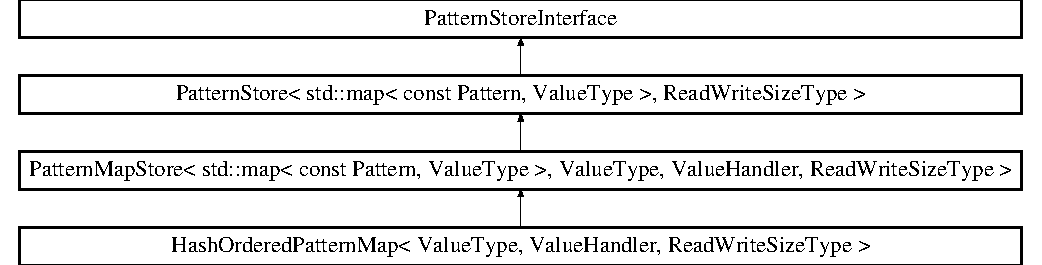
\includegraphics[height=3.561208cm]{classHashOrderedPatternMap}
\end{center}
\end{figure}
\subsection*{Public Types}
\begin{DoxyCompactItemize}
\item 
typedef std\+::map$<$ const \hyperlink{classPattern}{Pattern}, Value\+Type $>$\+::\hyperlink{classHashOrderedPatternMap_a149481ae49379713dae0ffcaff294f65}{iterator} \hyperlink{classHashOrderedPatternMap_a149481ae49379713dae0ffcaff294f65}{iterator}
\item 
typedef std\+::map$<$ const \hyperlink{classPattern}{Pattern}, Value\+Type $>$\+::\hyperlink{classHashOrderedPatternMap_a0162fc35654440e11ea66e71e8ffe8f8}{const\+\_\+iterator} \hyperlink{classHashOrderedPatternMap_a0162fc35654440e11ea66e71e8ffe8f8}{const\+\_\+iterator}
\end{DoxyCompactItemize}
\subsection*{Public Member Functions}
\begin{DoxyCompactItemize}
\item 
\hyperlink{classHashOrderedPatternMap_a8a1cb7250cb05276f9600af5283b376d}{Hash\+Ordered\+Pattern\+Map} ()
\item 
virtual \hyperlink{classHashOrderedPatternMap_a85d05fb0c6dcc95e7117c662967ccfdc}{$\sim$\+Hash\+Ordered\+Pattern\+Map} ()
\item 
void \hyperlink{classHashOrderedPatternMap_aec9cfa54723fbe49e75a4e93109ed0bf}{insert} (const \hyperlink{classPattern}{Pattern} \&pattern, Value\+Type \&value)
\item 
void \hyperlink{classHashOrderedPatternMap_a177fda1eb621d00266632cbf26025e8b}{insert} (const \hyperlink{classPattern}{Pattern} \&pattern)
\item 
bool \hyperlink{classHashOrderedPatternMap_a8682c2810f85d0c80ed015e388b571ef}{has} (const \hyperlink{classPattern}{Pattern} \&pattern) const 
\item 
bool \hyperlink{classHashOrderedPatternMap_ae2b83d2bcc1378b817044c205bd60651}{has} (const \hyperlink{classPatternPointer}{Pattern\+Pointer} \&pattern) const 
\item 
size\+\_\+t \hyperlink{classHashOrderedPatternMap_a5a48798964b7d667950f41630d3bf708}{size} () const 
\item 
Value\+Type \& \hyperlink{classHashOrderedPatternMap_ac37c92e91eb149eaa271054156264328}{operator\mbox{[}$\,$\mbox{]}} (const \hyperlink{classPattern}{Pattern} \&pattern)
\item 
Value\+Type \& \hyperlink{classHashOrderedPatternMap_a65a2aa5b240f6d88b205273331f212b9}{operator\mbox{[}$\,$\mbox{]}} (const \hyperlink{classPatternPointer}{Pattern\+Pointer} \&pattern)
\item 
\hyperlink{classHashOrderedPatternMap_a149481ae49379713dae0ffcaff294f65}{iterator} \hyperlink{classHashOrderedPatternMap_ac103913725b7036ba414453b2204b955}{begin} ()
\item 
\hyperlink{classHashOrderedPatternMap_a0162fc35654440e11ea66e71e8ffe8f8}{const\+\_\+iterator} \hyperlink{classHashOrderedPatternMap_a8bf9b181f9e7ed899ba48918af7a255d}{begin} () const 
\item 
\hyperlink{classHashOrderedPatternMap_a149481ae49379713dae0ffcaff294f65}{iterator} \hyperlink{classHashOrderedPatternMap_aa2a8090eed690299d4abeb36ea16fb3d}{end} ()
\item 
\hyperlink{classHashOrderedPatternMap_a0162fc35654440e11ea66e71e8ffe8f8}{const\+\_\+iterator} \hyperlink{classHashOrderedPatternMap_a0aa676a59fa89d30a0c477c193d7ceec}{end} () const 
\item 
\hyperlink{classHashOrderedPatternMap_a149481ae49379713dae0ffcaff294f65}{iterator} \hyperlink{classHashOrderedPatternMap_ab0391b67630d9c20ee0069f7197ca9da}{find} (const \hyperlink{classPattern}{Pattern} \&pattern)
\item 
\hyperlink{classHashOrderedPatternMap_a0162fc35654440e11ea66e71e8ffe8f8}{const\+\_\+iterator} \hyperlink{classHashOrderedPatternMap_aa3894103fb86543ab242d0da072afb56}{find} (const \hyperlink{classPattern}{Pattern} \&pattern) const 
\item 
bool \hyperlink{classHashOrderedPatternMap_acc3231c8b727c982ef11c80d3390f8ec}{erase} (const \hyperlink{classPattern}{Pattern} \&pattern)
\item 
\hyperlink{classHashOrderedPatternMap_a149481ae49379713dae0ffcaff294f65}{iterator} \hyperlink{classHashOrderedPatternMap_a3c9a41c27310278a2d2f02cc7016ebae}{erase} (\hyperlink{classHashOrderedPatternMap_a0162fc35654440e11ea66e71e8ffe8f8}{const\+\_\+iterator} position)
\end{DoxyCompactItemize}
\subsection*{Protected Attributes}
\begin{DoxyCompactItemize}
\item 
std\+::map$<$ const \hyperlink{classPattern}{Pattern}, Value\+Type $>$ \hyperlink{classHashOrderedPatternMap_adb4b3e32e897537d7bb1f5deaa650b7a}{data}
\end{DoxyCompactItemize}


\subsection{Member Typedef Documentation}
\hypertarget{classHashOrderedPatternMap_a0162fc35654440e11ea66e71e8ffe8f8}{}\index{Hash\+Ordered\+Pattern\+Map@{Hash\+Ordered\+Pattern\+Map}!const\+\_\+iterator@{const\+\_\+iterator}}
\index{const\+\_\+iterator@{const\+\_\+iterator}!Hash\+Ordered\+Pattern\+Map@{Hash\+Ordered\+Pattern\+Map}}
\subsubsection[{const\+\_\+iterator}]{\setlength{\rightskip}{0pt plus 5cm}template$<$class Value\+Type , class Value\+Handler  = Base\+Value\+Handler$<$\+Value\+Type$>$, class Read\+Write\+Size\+Type  = uint64\+\_\+t$>$ typedef std\+::map$<$const {\bf Pattern},Value\+Type$>$\+::{\bf const\+\_\+iterator} {\bf Hash\+Ordered\+Pattern\+Map}$<$ Value\+Type, Value\+Handler, Read\+Write\+Size\+Type $>$\+::{\bf const\+\_\+iterator}}\label{classHashOrderedPatternMap_a0162fc35654440e11ea66e71e8ffe8f8}
\hypertarget{classHashOrderedPatternMap_a149481ae49379713dae0ffcaff294f65}{}\index{Hash\+Ordered\+Pattern\+Map@{Hash\+Ordered\+Pattern\+Map}!iterator@{iterator}}
\index{iterator@{iterator}!Hash\+Ordered\+Pattern\+Map@{Hash\+Ordered\+Pattern\+Map}}
\subsubsection[{iterator}]{\setlength{\rightskip}{0pt plus 5cm}template$<$class Value\+Type , class Value\+Handler  = Base\+Value\+Handler$<$\+Value\+Type$>$, class Read\+Write\+Size\+Type  = uint64\+\_\+t$>$ typedef std\+::map$<$const {\bf Pattern},Value\+Type$>$\+::{\bf iterator} {\bf Hash\+Ordered\+Pattern\+Map}$<$ Value\+Type, Value\+Handler, Read\+Write\+Size\+Type $>$\+::{\bf iterator}}\label{classHashOrderedPatternMap_a149481ae49379713dae0ffcaff294f65}


\subsection{Constructor \& Destructor Documentation}
\hypertarget{classHashOrderedPatternMap_a8a1cb7250cb05276f9600af5283b376d}{}\index{Hash\+Ordered\+Pattern\+Map@{Hash\+Ordered\+Pattern\+Map}!Hash\+Ordered\+Pattern\+Map@{Hash\+Ordered\+Pattern\+Map}}
\index{Hash\+Ordered\+Pattern\+Map@{Hash\+Ordered\+Pattern\+Map}!Hash\+Ordered\+Pattern\+Map@{Hash\+Ordered\+Pattern\+Map}}
\subsubsection[{Hash\+Ordered\+Pattern\+Map()}]{\setlength{\rightskip}{0pt plus 5cm}template$<$class Value\+Type , class Value\+Handler  = Base\+Value\+Handler$<$\+Value\+Type$>$, class Read\+Write\+Size\+Type  = uint64\+\_\+t$>$ {\bf Hash\+Ordered\+Pattern\+Map}$<$ Value\+Type, Value\+Handler, Read\+Write\+Size\+Type $>$\+::{\bf Hash\+Ordered\+Pattern\+Map} (
\begin{DoxyParamCaption}
{}
\end{DoxyParamCaption}
)\hspace{0.3cm}{\ttfamily [inline]}}\label{classHashOrderedPatternMap_a8a1cb7250cb05276f9600af5283b376d}
\hypertarget{classHashOrderedPatternMap_a85d05fb0c6dcc95e7117c662967ccfdc}{}\index{Hash\+Ordered\+Pattern\+Map@{Hash\+Ordered\+Pattern\+Map}!````~Hash\+Ordered\+Pattern\+Map@{$\sim$\+Hash\+Ordered\+Pattern\+Map}}
\index{````~Hash\+Ordered\+Pattern\+Map@{$\sim$\+Hash\+Ordered\+Pattern\+Map}!Hash\+Ordered\+Pattern\+Map@{Hash\+Ordered\+Pattern\+Map}}
\subsubsection[{$\sim$\+Hash\+Ordered\+Pattern\+Map()}]{\setlength{\rightskip}{0pt plus 5cm}template$<$class Value\+Type , class Value\+Handler  = Base\+Value\+Handler$<$\+Value\+Type$>$, class Read\+Write\+Size\+Type  = uint64\+\_\+t$>$ virtual {\bf Hash\+Ordered\+Pattern\+Map}$<$ Value\+Type, Value\+Handler, Read\+Write\+Size\+Type $>$\+::$\sim${\bf Hash\+Ordered\+Pattern\+Map} (
\begin{DoxyParamCaption}
{}
\end{DoxyParamCaption}
)\hspace{0.3cm}{\ttfamily [inline]}, {\ttfamily [virtual]}}\label{classHashOrderedPatternMap_a85d05fb0c6dcc95e7117c662967ccfdc}


\subsection{Member Function Documentation}
\hypertarget{classHashOrderedPatternMap_ac103913725b7036ba414453b2204b955}{}\index{Hash\+Ordered\+Pattern\+Map@{Hash\+Ordered\+Pattern\+Map}!begin@{begin}}
\index{begin@{begin}!Hash\+Ordered\+Pattern\+Map@{Hash\+Ordered\+Pattern\+Map}}
\subsubsection[{begin()}]{\setlength{\rightskip}{0pt plus 5cm}template$<$class Value\+Type , class Value\+Handler  = Base\+Value\+Handler$<$\+Value\+Type$>$, class Read\+Write\+Size\+Type  = uint64\+\_\+t$>$ {\bf iterator} {\bf Hash\+Ordered\+Pattern\+Map}$<$ Value\+Type, Value\+Handler, Read\+Write\+Size\+Type $>$\+::begin (
\begin{DoxyParamCaption}
{}
\end{DoxyParamCaption}
)\hspace{0.3cm}{\ttfamily [inline]}, {\ttfamily [virtual]}}\label{classHashOrderedPatternMap_ac103913725b7036ba414453b2204b955}


Implements \hyperlink{classPatternMapStore_a2a0a8463a6faa2f2b6636167c06e19af}{Pattern\+Map\+Store$<$ std\+::map$<$ const Pattern, Value\+Type $>$, Value\+Type, Value\+Handler, Read\+Write\+Size\+Type $>$}.

\hypertarget{classHashOrderedPatternMap_a8bf9b181f9e7ed899ba48918af7a255d}{}\index{Hash\+Ordered\+Pattern\+Map@{Hash\+Ordered\+Pattern\+Map}!begin@{begin}}
\index{begin@{begin}!Hash\+Ordered\+Pattern\+Map@{Hash\+Ordered\+Pattern\+Map}}
\subsubsection[{begin() const }]{\setlength{\rightskip}{0pt plus 5cm}template$<$class Value\+Type , class Value\+Handler  = Base\+Value\+Handler$<$\+Value\+Type$>$, class Read\+Write\+Size\+Type  = uint64\+\_\+t$>$ {\bf const\+\_\+iterator} {\bf Hash\+Ordered\+Pattern\+Map}$<$ Value\+Type, Value\+Handler, Read\+Write\+Size\+Type $>$\+::begin (
\begin{DoxyParamCaption}
{}
\end{DoxyParamCaption}
) const\hspace{0.3cm}{\ttfamily [inline]}}\label{classHashOrderedPatternMap_a8bf9b181f9e7ed899ba48918af7a255d}
\hypertarget{classHashOrderedPatternMap_aa2a8090eed690299d4abeb36ea16fb3d}{}\index{Hash\+Ordered\+Pattern\+Map@{Hash\+Ordered\+Pattern\+Map}!end@{end}}
\index{end@{end}!Hash\+Ordered\+Pattern\+Map@{Hash\+Ordered\+Pattern\+Map}}
\subsubsection[{end()}]{\setlength{\rightskip}{0pt plus 5cm}template$<$class Value\+Type , class Value\+Handler  = Base\+Value\+Handler$<$\+Value\+Type$>$, class Read\+Write\+Size\+Type  = uint64\+\_\+t$>$ {\bf iterator} {\bf Hash\+Ordered\+Pattern\+Map}$<$ Value\+Type, Value\+Handler, Read\+Write\+Size\+Type $>$\+::end (
\begin{DoxyParamCaption}
{}
\end{DoxyParamCaption}
)\hspace{0.3cm}{\ttfamily [inline]}, {\ttfamily [virtual]}}\label{classHashOrderedPatternMap_aa2a8090eed690299d4abeb36ea16fb3d}


Implements \hyperlink{classPatternMapStore_a363c63981ea34474b28b2e3a95d376ce}{Pattern\+Map\+Store$<$ std\+::map$<$ const Pattern, Value\+Type $>$, Value\+Type, Value\+Handler, Read\+Write\+Size\+Type $>$}.

\hypertarget{classHashOrderedPatternMap_a0aa676a59fa89d30a0c477c193d7ceec}{}\index{Hash\+Ordered\+Pattern\+Map@{Hash\+Ordered\+Pattern\+Map}!end@{end}}
\index{end@{end}!Hash\+Ordered\+Pattern\+Map@{Hash\+Ordered\+Pattern\+Map}}
\subsubsection[{end() const }]{\setlength{\rightskip}{0pt plus 5cm}template$<$class Value\+Type , class Value\+Handler  = Base\+Value\+Handler$<$\+Value\+Type$>$, class Read\+Write\+Size\+Type  = uint64\+\_\+t$>$ {\bf const\+\_\+iterator} {\bf Hash\+Ordered\+Pattern\+Map}$<$ Value\+Type, Value\+Handler, Read\+Write\+Size\+Type $>$\+::end (
\begin{DoxyParamCaption}
{}
\end{DoxyParamCaption}
) const\hspace{0.3cm}{\ttfamily [inline]}}\label{classHashOrderedPatternMap_a0aa676a59fa89d30a0c477c193d7ceec}
\hypertarget{classHashOrderedPatternMap_acc3231c8b727c982ef11c80d3390f8ec}{}\index{Hash\+Ordered\+Pattern\+Map@{Hash\+Ordered\+Pattern\+Map}!erase@{erase}}
\index{erase@{erase}!Hash\+Ordered\+Pattern\+Map@{Hash\+Ordered\+Pattern\+Map}}
\subsubsection[{erase(const Pattern \&pattern)}]{\setlength{\rightskip}{0pt plus 5cm}template$<$class Value\+Type , class Value\+Handler  = Base\+Value\+Handler$<$\+Value\+Type$>$, class Read\+Write\+Size\+Type  = uint64\+\_\+t$>$ bool {\bf Hash\+Ordered\+Pattern\+Map}$<$ Value\+Type, Value\+Handler, Read\+Write\+Size\+Type $>$\+::erase (
\begin{DoxyParamCaption}
\item[{const {\bf Pattern} \&}]{pattern}
\end{DoxyParamCaption}
)\hspace{0.3cm}{\ttfamily [inline]}, {\ttfamily [virtual]}}\label{classHashOrderedPatternMap_acc3231c8b727c982ef11c80d3390f8ec}


Implements \hyperlink{classPatternMapStore_a60f2926144fbd408b86d9ff5481fd140}{Pattern\+Map\+Store$<$ std\+::map$<$ const Pattern, Value\+Type $>$, Value\+Type, Value\+Handler, Read\+Write\+Size\+Type $>$}.

\hypertarget{classHashOrderedPatternMap_a3c9a41c27310278a2d2f02cc7016ebae}{}\index{Hash\+Ordered\+Pattern\+Map@{Hash\+Ordered\+Pattern\+Map}!erase@{erase}}
\index{erase@{erase}!Hash\+Ordered\+Pattern\+Map@{Hash\+Ordered\+Pattern\+Map}}
\subsubsection[{erase(const\+\_\+iterator position)}]{\setlength{\rightskip}{0pt plus 5cm}template$<$class Value\+Type , class Value\+Handler  = Base\+Value\+Handler$<$\+Value\+Type$>$, class Read\+Write\+Size\+Type  = uint64\+\_\+t$>$ {\bf iterator} {\bf Hash\+Ordered\+Pattern\+Map}$<$ Value\+Type, Value\+Handler, Read\+Write\+Size\+Type $>$\+::erase (
\begin{DoxyParamCaption}
\item[{{\bf const\+\_\+iterator}}]{position}
\end{DoxyParamCaption}
)\hspace{0.3cm}{\ttfamily [inline]}}\label{classHashOrderedPatternMap_a3c9a41c27310278a2d2f02cc7016ebae}
\hypertarget{classHashOrderedPatternMap_ab0391b67630d9c20ee0069f7197ca9da}{}\index{Hash\+Ordered\+Pattern\+Map@{Hash\+Ordered\+Pattern\+Map}!find@{find}}
\index{find@{find}!Hash\+Ordered\+Pattern\+Map@{Hash\+Ordered\+Pattern\+Map}}
\subsubsection[{find(const Pattern \&pattern)}]{\setlength{\rightskip}{0pt plus 5cm}template$<$class Value\+Type , class Value\+Handler  = Base\+Value\+Handler$<$\+Value\+Type$>$, class Read\+Write\+Size\+Type  = uint64\+\_\+t$>$ {\bf iterator} {\bf Hash\+Ordered\+Pattern\+Map}$<$ Value\+Type, Value\+Handler, Read\+Write\+Size\+Type $>$\+::find (
\begin{DoxyParamCaption}
\item[{const {\bf Pattern} \&}]{pattern}
\end{DoxyParamCaption}
)\hspace{0.3cm}{\ttfamily [inline]}, {\ttfamily [virtual]}}\label{classHashOrderedPatternMap_ab0391b67630d9c20ee0069f7197ca9da}


Implements \hyperlink{classPatternMapStore_ae50e3cdbbf9a503d3381971daec92b54}{Pattern\+Map\+Store$<$ std\+::map$<$ const Pattern, Value\+Type $>$, Value\+Type, Value\+Handler, Read\+Write\+Size\+Type $>$}.

\hypertarget{classHashOrderedPatternMap_aa3894103fb86543ab242d0da072afb56}{}\index{Hash\+Ordered\+Pattern\+Map@{Hash\+Ordered\+Pattern\+Map}!find@{find}}
\index{find@{find}!Hash\+Ordered\+Pattern\+Map@{Hash\+Ordered\+Pattern\+Map}}
\subsubsection[{find(const Pattern \&pattern) const }]{\setlength{\rightskip}{0pt plus 5cm}template$<$class Value\+Type , class Value\+Handler  = Base\+Value\+Handler$<$\+Value\+Type$>$, class Read\+Write\+Size\+Type  = uint64\+\_\+t$>$ {\bf const\+\_\+iterator} {\bf Hash\+Ordered\+Pattern\+Map}$<$ Value\+Type, Value\+Handler, Read\+Write\+Size\+Type $>$\+::find (
\begin{DoxyParamCaption}
\item[{const {\bf Pattern} \&}]{pattern}
\end{DoxyParamCaption}
) const\hspace{0.3cm}{\ttfamily [inline]}}\label{classHashOrderedPatternMap_aa3894103fb86543ab242d0da072afb56}
\hypertarget{classHashOrderedPatternMap_a8682c2810f85d0c80ed015e388b571ef}{}\index{Hash\+Ordered\+Pattern\+Map@{Hash\+Ordered\+Pattern\+Map}!has@{has}}
\index{has@{has}!Hash\+Ordered\+Pattern\+Map@{Hash\+Ordered\+Pattern\+Map}}
\subsubsection[{has(const Pattern \&pattern) const }]{\setlength{\rightskip}{0pt plus 5cm}template$<$class Value\+Type , class Value\+Handler  = Base\+Value\+Handler$<$\+Value\+Type$>$, class Read\+Write\+Size\+Type  = uint64\+\_\+t$>$ bool {\bf Hash\+Ordered\+Pattern\+Map}$<$ Value\+Type, Value\+Handler, Read\+Write\+Size\+Type $>$\+::has (
\begin{DoxyParamCaption}
\item[{const {\bf Pattern} \&}]{}
\end{DoxyParamCaption}
) const\hspace{0.3cm}{\ttfamily [inline]}, {\ttfamily [virtual]}}\label{classHashOrderedPatternMap_a8682c2810f85d0c80ed015e388b571ef}
Does the pattern occur in the pattern store? 

Implements \hyperlink{classPatternMapStore_ad9c07c57785e95edbe057e79f94be2c9}{Pattern\+Map\+Store$<$ std\+::map$<$ const Pattern, Value\+Type $>$, Value\+Type, Value\+Handler, Read\+Write\+Size\+Type $>$}.

\hypertarget{classHashOrderedPatternMap_ae2b83d2bcc1378b817044c205bd60651}{}\index{Hash\+Ordered\+Pattern\+Map@{Hash\+Ordered\+Pattern\+Map}!has@{has}}
\index{has@{has}!Hash\+Ordered\+Pattern\+Map@{Hash\+Ordered\+Pattern\+Map}}
\subsubsection[{has(const Pattern\+Pointer \&pattern) const }]{\setlength{\rightskip}{0pt plus 5cm}template$<$class Value\+Type , class Value\+Handler  = Base\+Value\+Handler$<$\+Value\+Type$>$, class Read\+Write\+Size\+Type  = uint64\+\_\+t$>$ bool {\bf Hash\+Ordered\+Pattern\+Map}$<$ Value\+Type, Value\+Handler, Read\+Write\+Size\+Type $>$\+::has (
\begin{DoxyParamCaption}
\item[{const {\bf Pattern\+Pointer} \&}]{}
\end{DoxyParamCaption}
) const\hspace{0.3cm}{\ttfamily [inline]}, {\ttfamily [virtual]}}\label{classHashOrderedPatternMap_ae2b83d2bcc1378b817044c205bd60651}
Does the pattern occur in the pattern store? 

Implements \hyperlink{classPatternMapStore_a00d47f8640efaeb3ce85558b3ee4a6a2}{Pattern\+Map\+Store$<$ std\+::map$<$ const Pattern, Value\+Type $>$, Value\+Type, Value\+Handler, Read\+Write\+Size\+Type $>$}.

\hypertarget{classHashOrderedPatternMap_aec9cfa54723fbe49e75a4e93109ed0bf}{}\index{Hash\+Ordered\+Pattern\+Map@{Hash\+Ordered\+Pattern\+Map}!insert@{insert}}
\index{insert@{insert}!Hash\+Ordered\+Pattern\+Map@{Hash\+Ordered\+Pattern\+Map}}
\subsubsection[{insert(const Pattern \&pattern, Value\+Type \&value)}]{\setlength{\rightskip}{0pt plus 5cm}template$<$class Value\+Type , class Value\+Handler  = Base\+Value\+Handler$<$\+Value\+Type$>$, class Read\+Write\+Size\+Type  = uint64\+\_\+t$>$ void {\bf Hash\+Ordered\+Pattern\+Map}$<$ Value\+Type, Value\+Handler, Read\+Write\+Size\+Type $>$\+::insert (
\begin{DoxyParamCaption}
\item[{const {\bf Pattern} \&}]{pattern, }
\item[{Value\+Type \&}]{value}
\end{DoxyParamCaption}
)\hspace{0.3cm}{\ttfamily [inline]}, {\ttfamily [virtual]}}\label{classHashOrderedPatternMap_aec9cfa54723fbe49e75a4e93109ed0bf}


Implements \hyperlink{classPatternMapStore_a37bcf7aae1c40ccdea57e9a57533a555}{Pattern\+Map\+Store$<$ std\+::map$<$ const Pattern, Value\+Type $>$, Value\+Type, Value\+Handler, Read\+Write\+Size\+Type $>$}.

\hypertarget{classHashOrderedPatternMap_a177fda1eb621d00266632cbf26025e8b}{}\index{Hash\+Ordered\+Pattern\+Map@{Hash\+Ordered\+Pattern\+Map}!insert@{insert}}
\index{insert@{insert}!Hash\+Ordered\+Pattern\+Map@{Hash\+Ordered\+Pattern\+Map}}
\subsubsection[{insert(const Pattern \&pattern)}]{\setlength{\rightskip}{0pt plus 5cm}template$<$class Value\+Type , class Value\+Handler  = Base\+Value\+Handler$<$\+Value\+Type$>$, class Read\+Write\+Size\+Type  = uint64\+\_\+t$>$ void {\bf Hash\+Ordered\+Pattern\+Map}$<$ Value\+Type, Value\+Handler, Read\+Write\+Size\+Type $>$\+::insert (
\begin{DoxyParamCaption}
\item[{const {\bf Pattern} \&}]{pattern}
\end{DoxyParamCaption}
)\hspace{0.3cm}{\ttfamily [inline]}, {\ttfamily [virtual]}}\label{classHashOrderedPatternMap_a177fda1eb621d00266632cbf26025e8b}


Implements \hyperlink{classPatternStore_a22e091d80efb8182ac49cf6b225f0aa1}{Pattern\+Store$<$ std\+::map$<$ const Pattern, Value\+Type $>$, Read\+Write\+Size\+Type $>$}.

\hypertarget{classHashOrderedPatternMap_ac37c92e91eb149eaa271054156264328}{}\index{Hash\+Ordered\+Pattern\+Map@{Hash\+Ordered\+Pattern\+Map}!operator\mbox{[}$\,$\mbox{]}@{operator[]}}
\index{operator\mbox{[}$\,$\mbox{]}@{operator[]}!Hash\+Ordered\+Pattern\+Map@{Hash\+Ordered\+Pattern\+Map}}
\subsubsection[{operator[](const Pattern \&pattern)}]{\setlength{\rightskip}{0pt plus 5cm}template$<$class Value\+Type , class Value\+Handler  = Base\+Value\+Handler$<$\+Value\+Type$>$, class Read\+Write\+Size\+Type  = uint64\+\_\+t$>$ Value\+Type\& {\bf Hash\+Ordered\+Pattern\+Map}$<$ Value\+Type, Value\+Handler, Read\+Write\+Size\+Type $>$\+::operator\mbox{[}$\,$\mbox{]} (
\begin{DoxyParamCaption}
\item[{const {\bf Pattern} \&}]{pattern}
\end{DoxyParamCaption}
)\hspace{0.3cm}{\ttfamily [inline]}, {\ttfamily [virtual]}}\label{classHashOrderedPatternMap_ac37c92e91eb149eaa271054156264328}


Implements \hyperlink{classPatternMapStore_ac4e8b5a15bb4e3d0f205a979f0d272ab}{Pattern\+Map\+Store$<$ std\+::map$<$ const Pattern, Value\+Type $>$, Value\+Type, Value\+Handler, Read\+Write\+Size\+Type $>$}.

\hypertarget{classHashOrderedPatternMap_a65a2aa5b240f6d88b205273331f212b9}{}\index{Hash\+Ordered\+Pattern\+Map@{Hash\+Ordered\+Pattern\+Map}!operator\mbox{[}$\,$\mbox{]}@{operator[]}}
\index{operator\mbox{[}$\,$\mbox{]}@{operator[]}!Hash\+Ordered\+Pattern\+Map@{Hash\+Ordered\+Pattern\+Map}}
\subsubsection[{operator[](const Pattern\+Pointer \&pattern)}]{\setlength{\rightskip}{0pt plus 5cm}template$<$class Value\+Type , class Value\+Handler  = Base\+Value\+Handler$<$\+Value\+Type$>$, class Read\+Write\+Size\+Type  = uint64\+\_\+t$>$ Value\+Type\& {\bf Hash\+Ordered\+Pattern\+Map}$<$ Value\+Type, Value\+Handler, Read\+Write\+Size\+Type $>$\+::operator\mbox{[}$\,$\mbox{]} (
\begin{DoxyParamCaption}
\item[{const {\bf Pattern\+Pointer} \&}]{pattern}
\end{DoxyParamCaption}
)\hspace{0.3cm}{\ttfamily [inline]}, {\ttfamily [virtual]}}\label{classHashOrderedPatternMap_a65a2aa5b240f6d88b205273331f212b9}


Implements \hyperlink{classPatternMapStore_ac4f6c5ef2bd7397a33adeb2e72f6d38c}{Pattern\+Map\+Store$<$ std\+::map$<$ const Pattern, Value\+Type $>$, Value\+Type, Value\+Handler, Read\+Write\+Size\+Type $>$}.

\hypertarget{classHashOrderedPatternMap_a5a48798964b7d667950f41630d3bf708}{}\index{Hash\+Ordered\+Pattern\+Map@{Hash\+Ordered\+Pattern\+Map}!size@{size}}
\index{size@{size}!Hash\+Ordered\+Pattern\+Map@{Hash\+Ordered\+Pattern\+Map}}
\subsubsection[{size() const }]{\setlength{\rightskip}{0pt plus 5cm}template$<$class Value\+Type , class Value\+Handler  = Base\+Value\+Handler$<$\+Value\+Type$>$, class Read\+Write\+Size\+Type  = uint64\+\_\+t$>$ size\+\_\+t {\bf Hash\+Ordered\+Pattern\+Map}$<$ Value\+Type, Value\+Handler, Read\+Write\+Size\+Type $>$\+::size (
\begin{DoxyParamCaption}
{}
\end{DoxyParamCaption}
) const\hspace{0.3cm}{\ttfamily [inline]}, {\ttfamily [virtual]}}\label{classHashOrderedPatternMap_a5a48798964b7d667950f41630d3bf708}
How many patterns are in the pattern store? 

Implements \hyperlink{classPatternMapStore_ab6dc590b4b102f1464301a3fc6c4ec73}{Pattern\+Map\+Store$<$ std\+::map$<$ const Pattern, Value\+Type $>$, Value\+Type, Value\+Handler, Read\+Write\+Size\+Type $>$}.



\subsection{Member Data Documentation}
\hypertarget{classHashOrderedPatternMap_adb4b3e32e897537d7bb1f5deaa650b7a}{}\index{Hash\+Ordered\+Pattern\+Map@{Hash\+Ordered\+Pattern\+Map}!data@{data}}
\index{data@{data}!Hash\+Ordered\+Pattern\+Map@{Hash\+Ordered\+Pattern\+Map}}
\subsubsection[{data}]{\setlength{\rightskip}{0pt plus 5cm}template$<$class Value\+Type , class Value\+Handler  = Base\+Value\+Handler$<$\+Value\+Type$>$, class Read\+Write\+Size\+Type  = uint64\+\_\+t$>$ std\+::map$<$const {\bf Pattern}, Value\+Type$>$ {\bf Hash\+Ordered\+Pattern\+Map}$<$ Value\+Type, Value\+Handler, Read\+Write\+Size\+Type $>$\+::data\hspace{0.3cm}{\ttfamily [protected]}}\label{classHashOrderedPatternMap_adb4b3e32e897537d7bb1f5deaa650b7a}


The documentation for this class was generated from the following file\+:\begin{DoxyCompactItemize}
\item 
include/\hyperlink{patternstore_8h}{patternstore.\+h}\end{DoxyCompactItemize}

\hypertarget{classHashOrderedPatternSet}{}\section{Hash\+Ordered\+Pattern\+Set$<$ Read\+Write\+Size\+Type $>$ Class Template Reference}
\label{classHashOrderedPatternSet}\index{Hash\+Ordered\+Pattern\+Set$<$ Read\+Write\+Size\+Type $>$@{Hash\+Ordered\+Pattern\+Set$<$ Read\+Write\+Size\+Type $>$}}


A pattern store in the form of an ordered set (i.\+e, no duplicates). Stores only patterns, no values.  




{\ttfamily \#include $<$patternstore.\+h$>$}

Inheritance diagram for Hash\+Ordered\+Pattern\+Set$<$ Read\+Write\+Size\+Type $>$\+:\begin{figure}[H]
\begin{center}
\leavevmode
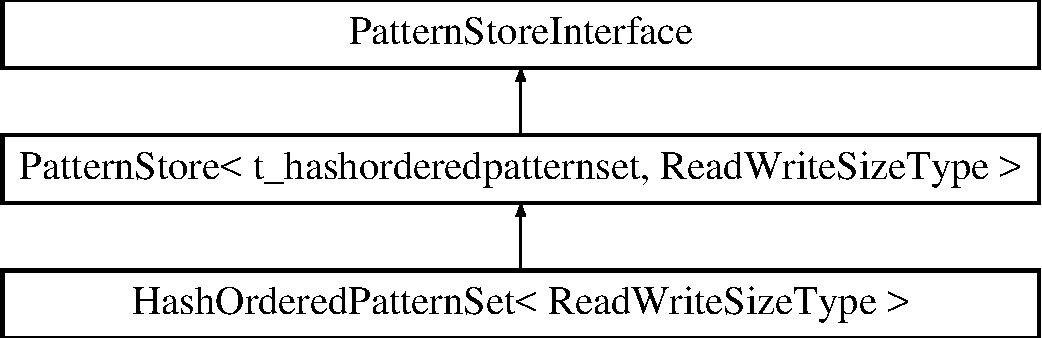
\includegraphics[height=3.000000cm]{classHashOrderedPatternSet}
\end{center}
\end{figure}
\subsection*{Public Types}
\begin{DoxyCompactItemize}
\item 
typedef t\+\_\+hashorderedpatternset\+::iterator \hyperlink{classHashOrderedPatternSet_a3191eb8aa122dfe2bf819d37468bd0b6}{iterator}
\item 
typedef t\+\_\+hashorderedpatternset\+::const\+\_\+iterator \hyperlink{classHashOrderedPatternSet_a5e1bbb1c4ef5ee0937bc0d5251a8d97e}{const\+\_\+iterator}
\end{DoxyCompactItemize}
\subsection*{Public Member Functions}
\begin{DoxyCompactItemize}
\item 
\hyperlink{classHashOrderedPatternSet_a045167c1a12c5e9e6dca775c2080a7b0}{Hash\+Ordered\+Pattern\+Set} ()
\item 
virtual \hyperlink{classHashOrderedPatternSet_acabae5fd5eb84ef383deb562a4cef808}{$\sim$\+Hash\+Ordered\+Pattern\+Set} ()
\item 
void \hyperlink{classHashOrderedPatternSet_a9da0aaf61e7b1425a181da16ccef6a1b}{insert} (const \hyperlink{classPattern}{Pattern} pattern)
\item 
bool \hyperlink{classHashOrderedPatternSet_ac21ec186302af16a3b70c5c85e434510}{has} (const \hyperlink{classPattern}{Pattern} \&pattern) const 
\item 
bool \hyperlink{classHashOrderedPatternSet_a4d917cedc8386b463aae0ad86856c82a}{has} (const \hyperlink{classPatternPointer}{Pattern\+Pointer} \&pattern) const 
\item 
size\+\_\+t \hyperlink{classHashOrderedPatternSet_a42fee5ee6f163edf807623ffc6ab2617}{size} () const 
\item 
void \hyperlink{classHashOrderedPatternSet_ac61b634d5e115949f2955dc85c3babe3}{reserve} (size\+\_\+t s)
\item 
\hyperlink{classHashOrderedPatternSet_a3191eb8aa122dfe2bf819d37468bd0b6}{iterator} \hyperlink{classHashOrderedPatternSet_a94bf915d870e33639c80839d7da7ce54}{begin} ()
\item 
\hyperlink{classHashOrderedPatternSet_a5e1bbb1c4ef5ee0937bc0d5251a8d97e}{const\+\_\+iterator} \hyperlink{classHashOrderedPatternSet_a82869ce8a41f6f5d45ffca4cd4f4133c}{begin} () const 
\item 
\hyperlink{classHashOrderedPatternSet_a3191eb8aa122dfe2bf819d37468bd0b6}{iterator} \hyperlink{classHashOrderedPatternSet_ada3bb2f1617443ad288c5c22dcd33ec0}{end} ()
\item 
\hyperlink{classHashOrderedPatternSet_a5e1bbb1c4ef5ee0937bc0d5251a8d97e}{const\+\_\+iterator} \hyperlink{classHashOrderedPatternSet_a0bd639de898189b047a8432292d18392}{end} () const 
\item 
\hyperlink{classHashOrderedPatternSet_a3191eb8aa122dfe2bf819d37468bd0b6}{iterator} \hyperlink{classHashOrderedPatternSet_aaf005777860a7af872aa104b1b7f9895}{find} (const \hyperlink{classPattern}{Pattern} \&pattern)
\item 
\hyperlink{classHashOrderedPatternSet_a5e1bbb1c4ef5ee0937bc0d5251a8d97e}{const\+\_\+iterator} \hyperlink{classHashOrderedPatternSet_a1c4db04fcfa32faf3f807f40bc52f602}{find} (const \hyperlink{classPattern}{Pattern} \&pattern) const 
\item 
\hyperlink{classHashOrderedPatternSet_a3191eb8aa122dfe2bf819d37468bd0b6}{iterator} \hyperlink{classHashOrderedPatternSet_a90e6642ea5198c48bb23af9cee8f3b76}{find} (const \hyperlink{classPatternPointer}{Pattern\+Pointer} \&pattern)
\item 
\hyperlink{classHashOrderedPatternSet_a5e1bbb1c4ef5ee0937bc0d5251a8d97e}{const\+\_\+iterator} \hyperlink{classHashOrderedPatternSet_af718bb8098b11ce4794815ccdf449ac6}{find} (const \hyperlink{classPatternPointer}{Pattern\+Pointer} \&pattern) const 
\item 
bool \hyperlink{classHashOrderedPatternSet_ab48e2380fcc00d9dc0ef01d9217fb5e6}{erase} (const \hyperlink{classPattern}{Pattern} \&pattern)
\item 
\hyperlink{classHashOrderedPatternSet_a3191eb8aa122dfe2bf819d37468bd0b6}{iterator} \hyperlink{classHashOrderedPatternSet_a6240dd699062a02b09811935517edab2}{erase} (\hyperlink{classHashOrderedPatternSet_a5e1bbb1c4ef5ee0937bc0d5251a8d97e}{const\+\_\+iterator} position)
\item 
void \hyperlink{classHashOrderedPatternSet_a5410dc1022729fe531e7ef7dcd0e845c}{write} (std\+::ostream $\ast$out)
\item 
void \hyperlink{classHashOrderedPatternSet_ae4f18bc4f126da615a0ec194fe8f24b0}{read} (std\+::istream $\ast$in, int M\+I\+N\+L\+E\+N\+G\+T\+H=0, int M\+A\+X\+L\+E\+N\+G\+T\+H=999999, bool D\+O\+N\+G\+R\+A\+M\+S=true, bool D\+O\+S\+K\+I\+P\+G\+R\+A\+M\+S=true, bool D\+O\+F\+L\+E\+X\+G\+R\+A\+M\+S=true)
\end{DoxyCompactItemize}
\subsection*{Protected Attributes}
\begin{DoxyCompactItemize}
\item 
\hyperlink{patternstore_8h_a95f03de9f728d05eb31111e2dbdac6a7}{t\+\_\+hashorderedpatternset} \hyperlink{classHashOrderedPatternSet_a04f495b51e93c8f7d6798623398e5e61}{data}
\end{DoxyCompactItemize}


\subsection{Detailed Description}
\subsubsection*{template$<$class Read\+Write\+Size\+Type = uint64\+\_\+t$>$class Hash\+Ordered\+Pattern\+Set$<$ Read\+Write\+Size\+Type $>$}

A pattern store in the form of an ordered set (i.\+e, no duplicates). Stores only patterns, no values. 


\begin{DoxyTemplParams}{Template Parameters}
{\em Read\+Write\+Size\+Type} & The data type for addressing, determines the maximum amount of patterns that can be held, only used in serialisation/deserialisation \\
\hline
\end{DoxyTemplParams}


\subsection{Member Typedef Documentation}
\hypertarget{classHashOrderedPatternSet_a5e1bbb1c4ef5ee0937bc0d5251a8d97e}{}\index{Hash\+Ordered\+Pattern\+Set@{Hash\+Ordered\+Pattern\+Set}!const\+\_\+iterator@{const\+\_\+iterator}}
\index{const\+\_\+iterator@{const\+\_\+iterator}!Hash\+Ordered\+Pattern\+Set@{Hash\+Ordered\+Pattern\+Set}}
\subsubsection[{const\+\_\+iterator}]{\setlength{\rightskip}{0pt plus 5cm}template$<$class Read\+Write\+Size\+Type  = uint64\+\_\+t$>$ typedef t\+\_\+hashorderedpatternset\+::const\+\_\+iterator {\bf Hash\+Ordered\+Pattern\+Set}$<$ Read\+Write\+Size\+Type $>$\+::{\bf const\+\_\+iterator}}\label{classHashOrderedPatternSet_a5e1bbb1c4ef5ee0937bc0d5251a8d97e}
\hypertarget{classHashOrderedPatternSet_a3191eb8aa122dfe2bf819d37468bd0b6}{}\index{Hash\+Ordered\+Pattern\+Set@{Hash\+Ordered\+Pattern\+Set}!iterator@{iterator}}
\index{iterator@{iterator}!Hash\+Ordered\+Pattern\+Set@{Hash\+Ordered\+Pattern\+Set}}
\subsubsection[{iterator}]{\setlength{\rightskip}{0pt plus 5cm}template$<$class Read\+Write\+Size\+Type  = uint64\+\_\+t$>$ typedef t\+\_\+hashorderedpatternset\+::iterator {\bf Hash\+Ordered\+Pattern\+Set}$<$ Read\+Write\+Size\+Type $>$\+::{\bf iterator}}\label{classHashOrderedPatternSet_a3191eb8aa122dfe2bf819d37468bd0b6}


\subsection{Constructor \& Destructor Documentation}
\hypertarget{classHashOrderedPatternSet_a045167c1a12c5e9e6dca775c2080a7b0}{}\index{Hash\+Ordered\+Pattern\+Set@{Hash\+Ordered\+Pattern\+Set}!Hash\+Ordered\+Pattern\+Set@{Hash\+Ordered\+Pattern\+Set}}
\index{Hash\+Ordered\+Pattern\+Set@{Hash\+Ordered\+Pattern\+Set}!Hash\+Ordered\+Pattern\+Set@{Hash\+Ordered\+Pattern\+Set}}
\subsubsection[{Hash\+Ordered\+Pattern\+Set()}]{\setlength{\rightskip}{0pt plus 5cm}template$<$class Read\+Write\+Size\+Type  = uint64\+\_\+t$>$ {\bf Hash\+Ordered\+Pattern\+Set}$<$ Read\+Write\+Size\+Type $>$\+::{\bf Hash\+Ordered\+Pattern\+Set} (
\begin{DoxyParamCaption}
{}
\end{DoxyParamCaption}
)\hspace{0.3cm}{\ttfamily [inline]}}\label{classHashOrderedPatternSet_a045167c1a12c5e9e6dca775c2080a7b0}
\hypertarget{classHashOrderedPatternSet_acabae5fd5eb84ef383deb562a4cef808}{}\index{Hash\+Ordered\+Pattern\+Set@{Hash\+Ordered\+Pattern\+Set}!````~Hash\+Ordered\+Pattern\+Set@{$\sim$\+Hash\+Ordered\+Pattern\+Set}}
\index{````~Hash\+Ordered\+Pattern\+Set@{$\sim$\+Hash\+Ordered\+Pattern\+Set}!Hash\+Ordered\+Pattern\+Set@{Hash\+Ordered\+Pattern\+Set}}
\subsubsection[{$\sim$\+Hash\+Ordered\+Pattern\+Set()}]{\setlength{\rightskip}{0pt plus 5cm}template$<$class Read\+Write\+Size\+Type  = uint64\+\_\+t$>$ virtual {\bf Hash\+Ordered\+Pattern\+Set}$<$ Read\+Write\+Size\+Type $>$\+::$\sim${\bf Hash\+Ordered\+Pattern\+Set} (
\begin{DoxyParamCaption}
{}
\end{DoxyParamCaption}
)\hspace{0.3cm}{\ttfamily [virtual]}}\label{classHashOrderedPatternSet_acabae5fd5eb84ef383deb562a4cef808}


\subsection{Member Function Documentation}
\hypertarget{classHashOrderedPatternSet_a94bf915d870e33639c80839d7da7ce54}{}\index{Hash\+Ordered\+Pattern\+Set@{Hash\+Ordered\+Pattern\+Set}!begin@{begin}}
\index{begin@{begin}!Hash\+Ordered\+Pattern\+Set@{Hash\+Ordered\+Pattern\+Set}}
\subsubsection[{begin()}]{\setlength{\rightskip}{0pt plus 5cm}template$<$class Read\+Write\+Size\+Type  = uint64\+\_\+t$>$ {\bf iterator} {\bf Hash\+Ordered\+Pattern\+Set}$<$ Read\+Write\+Size\+Type $>$\+::begin (
\begin{DoxyParamCaption}
{}
\end{DoxyParamCaption}
)\hspace{0.3cm}{\ttfamily [inline]}, {\ttfamily [virtual]}}\label{classHashOrderedPatternSet_a94bf915d870e33639c80839d7da7ce54}


Implements \hyperlink{classPatternStore_aab3fab217b585b2b90a3fb3cc7065e11}{Pattern\+Store$<$ t\+\_\+hashorderedpatternset, Read\+Write\+Size\+Type $>$}.

\hypertarget{classHashOrderedPatternSet_a82869ce8a41f6f5d45ffca4cd4f4133c}{}\index{Hash\+Ordered\+Pattern\+Set@{Hash\+Ordered\+Pattern\+Set}!begin@{begin}}
\index{begin@{begin}!Hash\+Ordered\+Pattern\+Set@{Hash\+Ordered\+Pattern\+Set}}
\subsubsection[{begin() const }]{\setlength{\rightskip}{0pt plus 5cm}template$<$class Read\+Write\+Size\+Type  = uint64\+\_\+t$>$ {\bf const\+\_\+iterator} {\bf Hash\+Ordered\+Pattern\+Set}$<$ Read\+Write\+Size\+Type $>$\+::begin (
\begin{DoxyParamCaption}
{}
\end{DoxyParamCaption}
) const\hspace{0.3cm}{\ttfamily [inline]}}\label{classHashOrderedPatternSet_a82869ce8a41f6f5d45ffca4cd4f4133c}
\hypertarget{classHashOrderedPatternSet_ada3bb2f1617443ad288c5c22dcd33ec0}{}\index{Hash\+Ordered\+Pattern\+Set@{Hash\+Ordered\+Pattern\+Set}!end@{end}}
\index{end@{end}!Hash\+Ordered\+Pattern\+Set@{Hash\+Ordered\+Pattern\+Set}}
\subsubsection[{end()}]{\setlength{\rightskip}{0pt plus 5cm}template$<$class Read\+Write\+Size\+Type  = uint64\+\_\+t$>$ {\bf iterator} {\bf Hash\+Ordered\+Pattern\+Set}$<$ Read\+Write\+Size\+Type $>$\+::end (
\begin{DoxyParamCaption}
{}
\end{DoxyParamCaption}
)\hspace{0.3cm}{\ttfamily [inline]}, {\ttfamily [virtual]}}\label{classHashOrderedPatternSet_ada3bb2f1617443ad288c5c22dcd33ec0}


Implements \hyperlink{classPatternStore_ae697b6ba815e09fa300532a78e1c9077}{Pattern\+Store$<$ t\+\_\+hashorderedpatternset, Read\+Write\+Size\+Type $>$}.

\hypertarget{classHashOrderedPatternSet_a0bd639de898189b047a8432292d18392}{}\index{Hash\+Ordered\+Pattern\+Set@{Hash\+Ordered\+Pattern\+Set}!end@{end}}
\index{end@{end}!Hash\+Ordered\+Pattern\+Set@{Hash\+Ordered\+Pattern\+Set}}
\subsubsection[{end() const }]{\setlength{\rightskip}{0pt plus 5cm}template$<$class Read\+Write\+Size\+Type  = uint64\+\_\+t$>$ {\bf const\+\_\+iterator} {\bf Hash\+Ordered\+Pattern\+Set}$<$ Read\+Write\+Size\+Type $>$\+::end (
\begin{DoxyParamCaption}
{}
\end{DoxyParamCaption}
) const\hspace{0.3cm}{\ttfamily [inline]}}\label{classHashOrderedPatternSet_a0bd639de898189b047a8432292d18392}
\hypertarget{classHashOrderedPatternSet_ab48e2380fcc00d9dc0ef01d9217fb5e6}{}\index{Hash\+Ordered\+Pattern\+Set@{Hash\+Ordered\+Pattern\+Set}!erase@{erase}}
\index{erase@{erase}!Hash\+Ordered\+Pattern\+Set@{Hash\+Ordered\+Pattern\+Set}}
\subsubsection[{erase(const Pattern \&pattern)}]{\setlength{\rightskip}{0pt plus 5cm}template$<$class Read\+Write\+Size\+Type  = uint64\+\_\+t$>$ bool {\bf Hash\+Ordered\+Pattern\+Set}$<$ Read\+Write\+Size\+Type $>$\+::erase (
\begin{DoxyParamCaption}
\item[{const {\bf Pattern} \&}]{pattern}
\end{DoxyParamCaption}
)\hspace{0.3cm}{\ttfamily [inline]}, {\ttfamily [virtual]}}\label{classHashOrderedPatternSet_ab48e2380fcc00d9dc0ef01d9217fb5e6}


Implements \hyperlink{classPatternStore_a42f8de80a8627c485315e4bb8eff538f}{Pattern\+Store$<$ t\+\_\+hashorderedpatternset, Read\+Write\+Size\+Type $>$}.

\hypertarget{classHashOrderedPatternSet_a6240dd699062a02b09811935517edab2}{}\index{Hash\+Ordered\+Pattern\+Set@{Hash\+Ordered\+Pattern\+Set}!erase@{erase}}
\index{erase@{erase}!Hash\+Ordered\+Pattern\+Set@{Hash\+Ordered\+Pattern\+Set}}
\subsubsection[{erase(const\+\_\+iterator position)}]{\setlength{\rightskip}{0pt plus 5cm}template$<$class Read\+Write\+Size\+Type  = uint64\+\_\+t$>$ {\bf iterator} {\bf Hash\+Ordered\+Pattern\+Set}$<$ Read\+Write\+Size\+Type $>$\+::erase (
\begin{DoxyParamCaption}
\item[{{\bf const\+\_\+iterator}}]{position}
\end{DoxyParamCaption}
)\hspace{0.3cm}{\ttfamily [inline]}}\label{classHashOrderedPatternSet_a6240dd699062a02b09811935517edab2}
\hypertarget{classHashOrderedPatternSet_aaf005777860a7af872aa104b1b7f9895}{}\index{Hash\+Ordered\+Pattern\+Set@{Hash\+Ordered\+Pattern\+Set}!find@{find}}
\index{find@{find}!Hash\+Ordered\+Pattern\+Set@{Hash\+Ordered\+Pattern\+Set}}
\subsubsection[{find(const Pattern \&pattern)}]{\setlength{\rightskip}{0pt plus 5cm}template$<$class Read\+Write\+Size\+Type  = uint64\+\_\+t$>$ {\bf iterator} {\bf Hash\+Ordered\+Pattern\+Set}$<$ Read\+Write\+Size\+Type $>$\+::find (
\begin{DoxyParamCaption}
\item[{const {\bf Pattern} \&}]{pattern}
\end{DoxyParamCaption}
)\hspace{0.3cm}{\ttfamily [inline]}, {\ttfamily [virtual]}}\label{classHashOrderedPatternSet_aaf005777860a7af872aa104b1b7f9895}


Implements \hyperlink{classPatternStore_a6996798c63c2dd3ae3845848da35a6dd}{Pattern\+Store$<$ t\+\_\+hashorderedpatternset, Read\+Write\+Size\+Type $>$}.

\hypertarget{classHashOrderedPatternSet_a1c4db04fcfa32faf3f807f40bc52f602}{}\index{Hash\+Ordered\+Pattern\+Set@{Hash\+Ordered\+Pattern\+Set}!find@{find}}
\index{find@{find}!Hash\+Ordered\+Pattern\+Set@{Hash\+Ordered\+Pattern\+Set}}
\subsubsection[{find(const Pattern \&pattern) const }]{\setlength{\rightskip}{0pt plus 5cm}template$<$class Read\+Write\+Size\+Type  = uint64\+\_\+t$>$ {\bf const\+\_\+iterator} {\bf Hash\+Ordered\+Pattern\+Set}$<$ Read\+Write\+Size\+Type $>$\+::find (
\begin{DoxyParamCaption}
\item[{const {\bf Pattern} \&}]{pattern}
\end{DoxyParamCaption}
) const\hspace{0.3cm}{\ttfamily [inline]}}\label{classHashOrderedPatternSet_a1c4db04fcfa32faf3f807f40bc52f602}
\hypertarget{classHashOrderedPatternSet_a90e6642ea5198c48bb23af9cee8f3b76}{}\index{Hash\+Ordered\+Pattern\+Set@{Hash\+Ordered\+Pattern\+Set}!find@{find}}
\index{find@{find}!Hash\+Ordered\+Pattern\+Set@{Hash\+Ordered\+Pattern\+Set}}
\subsubsection[{find(const Pattern\+Pointer \&pattern)}]{\setlength{\rightskip}{0pt plus 5cm}template$<$class Read\+Write\+Size\+Type  = uint64\+\_\+t$>$ {\bf iterator} {\bf Hash\+Ordered\+Pattern\+Set}$<$ Read\+Write\+Size\+Type $>$\+::find (
\begin{DoxyParamCaption}
\item[{const {\bf Pattern\+Pointer} \&}]{pattern}
\end{DoxyParamCaption}
)\hspace{0.3cm}{\ttfamily [inline]}, {\ttfamily [virtual]}}\label{classHashOrderedPatternSet_a90e6642ea5198c48bb23af9cee8f3b76}


Implements \hyperlink{classPatternStore_a33991d30a74b13a4264200474bf0542c}{Pattern\+Store$<$ t\+\_\+hashorderedpatternset, Read\+Write\+Size\+Type $>$}.

\hypertarget{classHashOrderedPatternSet_af718bb8098b11ce4794815ccdf449ac6}{}\index{Hash\+Ordered\+Pattern\+Set@{Hash\+Ordered\+Pattern\+Set}!find@{find}}
\index{find@{find}!Hash\+Ordered\+Pattern\+Set@{Hash\+Ordered\+Pattern\+Set}}
\subsubsection[{find(const Pattern\+Pointer \&pattern) const }]{\setlength{\rightskip}{0pt plus 5cm}template$<$class Read\+Write\+Size\+Type  = uint64\+\_\+t$>$ {\bf const\+\_\+iterator} {\bf Hash\+Ordered\+Pattern\+Set}$<$ Read\+Write\+Size\+Type $>$\+::find (
\begin{DoxyParamCaption}
\item[{const {\bf Pattern\+Pointer} \&}]{pattern}
\end{DoxyParamCaption}
) const\hspace{0.3cm}{\ttfamily [inline]}}\label{classHashOrderedPatternSet_af718bb8098b11ce4794815ccdf449ac6}
\hypertarget{classHashOrderedPatternSet_ac21ec186302af16a3b70c5c85e434510}{}\index{Hash\+Ordered\+Pattern\+Set@{Hash\+Ordered\+Pattern\+Set}!has@{has}}
\index{has@{has}!Hash\+Ordered\+Pattern\+Set@{Hash\+Ordered\+Pattern\+Set}}
\subsubsection[{has(const Pattern \&pattern) const }]{\setlength{\rightskip}{0pt plus 5cm}template$<$class Read\+Write\+Size\+Type  = uint64\+\_\+t$>$ bool {\bf Hash\+Ordered\+Pattern\+Set}$<$ Read\+Write\+Size\+Type $>$\+::has (
\begin{DoxyParamCaption}
\item[{const {\bf Pattern} \&}]{}
\end{DoxyParamCaption}
) const\hspace{0.3cm}{\ttfamily [inline]}, {\ttfamily [virtual]}}\label{classHashOrderedPatternSet_ac21ec186302af16a3b70c5c85e434510}
Does the pattern occur in the pattern store? 

Implements \hyperlink{classPatternStore_a2e29add9b35b3459d183f56f6c5525ed}{Pattern\+Store$<$ t\+\_\+hashorderedpatternset, Read\+Write\+Size\+Type $>$}.

\hypertarget{classHashOrderedPatternSet_a4d917cedc8386b463aae0ad86856c82a}{}\index{Hash\+Ordered\+Pattern\+Set@{Hash\+Ordered\+Pattern\+Set}!has@{has}}
\index{has@{has}!Hash\+Ordered\+Pattern\+Set@{Hash\+Ordered\+Pattern\+Set}}
\subsubsection[{has(const Pattern\+Pointer \&pattern) const }]{\setlength{\rightskip}{0pt plus 5cm}template$<$class Read\+Write\+Size\+Type  = uint64\+\_\+t$>$ bool {\bf Hash\+Ordered\+Pattern\+Set}$<$ Read\+Write\+Size\+Type $>$\+::has (
\begin{DoxyParamCaption}
\item[{const {\bf Pattern\+Pointer} \&}]{}
\end{DoxyParamCaption}
) const\hspace{0.3cm}{\ttfamily [inline]}, {\ttfamily [virtual]}}\label{classHashOrderedPatternSet_a4d917cedc8386b463aae0ad86856c82a}
Does the pattern occur in the pattern store? 

Implements \hyperlink{classPatternStore_ad1e06c2468bad2a14d4ed28b26c6ff33}{Pattern\+Store$<$ t\+\_\+hashorderedpatternset, Read\+Write\+Size\+Type $>$}.

\hypertarget{classHashOrderedPatternSet_a9da0aaf61e7b1425a181da16ccef6a1b}{}\index{Hash\+Ordered\+Pattern\+Set@{Hash\+Ordered\+Pattern\+Set}!insert@{insert}}
\index{insert@{insert}!Hash\+Ordered\+Pattern\+Set@{Hash\+Ordered\+Pattern\+Set}}
\subsubsection[{insert(const Pattern pattern)}]{\setlength{\rightskip}{0pt plus 5cm}template$<$class Read\+Write\+Size\+Type  = uint64\+\_\+t$>$ void {\bf Hash\+Ordered\+Pattern\+Set}$<$ Read\+Write\+Size\+Type $>$\+::insert (
\begin{DoxyParamCaption}
\item[{const {\bf Pattern}}]{pattern}
\end{DoxyParamCaption}
)\hspace{0.3cm}{\ttfamily [inline]}}\label{classHashOrderedPatternSet_a9da0aaf61e7b1425a181da16ccef6a1b}
\hypertarget{classHashOrderedPatternSet_ae4f18bc4f126da615a0ec194fe8f24b0}{}\index{Hash\+Ordered\+Pattern\+Set@{Hash\+Ordered\+Pattern\+Set}!read@{read}}
\index{read@{read}!Hash\+Ordered\+Pattern\+Set@{Hash\+Ordered\+Pattern\+Set}}
\subsubsection[{read(std\+::istream $\ast$in, int M\+I\+N\+L\+E\+N\+G\+T\+H=0, int M\+A\+X\+L\+E\+N\+G\+T\+H=999999, bool D\+O\+N\+G\+R\+A\+M\+S=true, bool D\+O\+S\+K\+I\+P\+G\+R\+A\+M\+S=true, bool D\+O\+F\+L\+E\+X\+G\+R\+A\+M\+S=true)}]{\setlength{\rightskip}{0pt plus 5cm}template$<$class Read\+Write\+Size\+Type  = uint64\+\_\+t$>$ void {\bf Hash\+Ordered\+Pattern\+Set}$<$ Read\+Write\+Size\+Type $>$\+::read (
\begin{DoxyParamCaption}
\item[{std\+::istream $\ast$}]{in, }
\item[{int}]{M\+I\+N\+L\+E\+N\+G\+T\+H = {\ttfamily 0}, }
\item[{int}]{M\+A\+X\+L\+E\+N\+G\+T\+H = {\ttfamily 999999}, }
\item[{bool}]{D\+O\+N\+G\+R\+A\+M\+S = {\ttfamily true}, }
\item[{bool}]{D\+O\+S\+K\+I\+P\+G\+R\+A\+M\+S = {\ttfamily true}, }
\item[{bool}]{D\+O\+F\+L\+E\+X\+G\+R\+A\+M\+S = {\ttfamily true}}
\end{DoxyParamCaption}
)\hspace{0.3cm}{\ttfamily [inline]}}\label{classHashOrderedPatternSet_ae4f18bc4f126da615a0ec194fe8f24b0}
\hypertarget{classHashOrderedPatternSet_ac61b634d5e115949f2955dc85c3babe3}{}\index{Hash\+Ordered\+Pattern\+Set@{Hash\+Ordered\+Pattern\+Set}!reserve@{reserve}}
\index{reserve@{reserve}!Hash\+Ordered\+Pattern\+Set@{Hash\+Ordered\+Pattern\+Set}}
\subsubsection[{reserve(size\+\_\+t s)}]{\setlength{\rightskip}{0pt plus 5cm}template$<$class Read\+Write\+Size\+Type  = uint64\+\_\+t$>$ void {\bf Hash\+Ordered\+Pattern\+Set}$<$ Read\+Write\+Size\+Type $>$\+::reserve (
\begin{DoxyParamCaption}
\item[{size\+\_\+t}]{s}
\end{DoxyParamCaption}
)\hspace{0.3cm}{\ttfamily [inline]}, {\ttfamily [virtual]}}\label{classHashOrderedPatternSet_ac61b634d5e115949f2955dc85c3babe3}


Implements \hyperlink{classPatternStore_afc995f7b88b6a31b700bb3bdb948b180}{Pattern\+Store$<$ t\+\_\+hashorderedpatternset, Read\+Write\+Size\+Type $>$}.

\hypertarget{classHashOrderedPatternSet_a42fee5ee6f163edf807623ffc6ab2617}{}\index{Hash\+Ordered\+Pattern\+Set@{Hash\+Ordered\+Pattern\+Set}!size@{size}}
\index{size@{size}!Hash\+Ordered\+Pattern\+Set@{Hash\+Ordered\+Pattern\+Set}}
\subsubsection[{size() const }]{\setlength{\rightskip}{0pt plus 5cm}template$<$class Read\+Write\+Size\+Type  = uint64\+\_\+t$>$ size\+\_\+t {\bf Hash\+Ordered\+Pattern\+Set}$<$ Read\+Write\+Size\+Type $>$\+::size (
\begin{DoxyParamCaption}
{}
\end{DoxyParamCaption}
) const\hspace{0.3cm}{\ttfamily [inline]}, {\ttfamily [virtual]}}\label{classHashOrderedPatternSet_a42fee5ee6f163edf807623ffc6ab2617}
How many patterns are in the pattern store? 

Implements \hyperlink{classPatternStore_abfa82df94ab565bea13fc45ee4866faf}{Pattern\+Store$<$ t\+\_\+hashorderedpatternset, Read\+Write\+Size\+Type $>$}.

\hypertarget{classHashOrderedPatternSet_a5410dc1022729fe531e7ef7dcd0e845c}{}\index{Hash\+Ordered\+Pattern\+Set@{Hash\+Ordered\+Pattern\+Set}!write@{write}}
\index{write@{write}!Hash\+Ordered\+Pattern\+Set@{Hash\+Ordered\+Pattern\+Set}}
\subsubsection[{write(std\+::ostream $\ast$out)}]{\setlength{\rightskip}{0pt plus 5cm}template$<$class Read\+Write\+Size\+Type  = uint64\+\_\+t$>$ void {\bf Hash\+Ordered\+Pattern\+Set}$<$ Read\+Write\+Size\+Type $>$\+::write (
\begin{DoxyParamCaption}
\item[{std\+::ostream $\ast$}]{out}
\end{DoxyParamCaption}
)\hspace{0.3cm}{\ttfamily [inline]}, {\ttfamily [virtual]}}\label{classHashOrderedPatternSet_a5410dc1022729fe531e7ef7dcd0e845c}


Implements \hyperlink{classPatternStore_a70d9b8faa5858ab7182cea7b1488a75c}{Pattern\+Store$<$ t\+\_\+hashorderedpatternset, Read\+Write\+Size\+Type $>$}.



\subsection{Member Data Documentation}
\hypertarget{classHashOrderedPatternSet_a04f495b51e93c8f7d6798623398e5e61}{}\index{Hash\+Ordered\+Pattern\+Set@{Hash\+Ordered\+Pattern\+Set}!data@{data}}
\index{data@{data}!Hash\+Ordered\+Pattern\+Set@{Hash\+Ordered\+Pattern\+Set}}
\subsubsection[{data}]{\setlength{\rightskip}{0pt plus 5cm}template$<$class Read\+Write\+Size\+Type  = uint64\+\_\+t$>$ {\bf t\+\_\+hashorderedpatternset} {\bf Hash\+Ordered\+Pattern\+Set}$<$ Read\+Write\+Size\+Type $>$\+::data\hspace{0.3cm}{\ttfamily [protected]}}\label{classHashOrderedPatternSet_a04f495b51e93c8f7d6798623398e5e61}


The documentation for this class was generated from the following file\+:\begin{DoxyCompactItemize}
\item 
include/\hyperlink{patternstore_8h}{patternstore.\+h}\end{DoxyCompactItemize}

\hypertarget{classIndexedCorpus}{}\section{Indexed\+Corpus Class Reference}
\label{classIndexedCorpus}\index{Indexed\+Corpus@{Indexed\+Corpus}}


Class for reading an entire (class encoded) corpus into memory. It provides a reverse index by \hyperlink{classIndexReference}{Index\+Reference}. The reverse index stores positions and unigrams.  




{\ttfamily \#include $<$patternstore.\+h$>$}

\subsection*{Classes}
\begin{DoxyCompactItemize}
\item 
class \hyperlink{classIndexedCorpus_1_1iterator}{iterator}
\end{DoxyCompactItemize}
\subsection*{Public Member Functions}
\begin{DoxyCompactItemize}
\item 
\hyperlink{classIndexedCorpus_abed3d107618b4d1cc91f77c56445c5a5}{Indexed\+Corpus} ()
\item 
\hyperlink{classIndexedCorpus_a90eaf21374d0bc17af480c882fcb07b2}{Indexed\+Corpus} (unsigned char $\ast$\hyperlink{classIndexedCorpus_a382d8734879b170282345a5e20e71113}{corpus}, unsigned int \hyperlink{classIndexedCorpus_aaea6690e61d8538ae86f62857f044563}{corpussize})
\item 
\hyperlink{classIndexedCorpus_a3a2369b02abd0c7f4eb25710a5aec446}{Indexed\+Corpus} (std\+::istream $\ast$in, bool debug=false)
\item 
\hyperlink{classIndexedCorpus_ab5d67abefdab495addd6bdfb976c4c0b}{Indexed\+Corpus} (std\+::string filename, bool debug=false)
\item 
\hyperlink{classIndexedCorpus_ae6bbb800f2a974b60336be7e0678ae91}{$\sim$\+Indexed\+Corpus} ()
\item 
void \hyperlink{classIndexedCorpus_af77786d6aba870b93e5cea36e25842c2}{load} (std\+::istream $\ast$in, bool debug=false)
\item 
void \hyperlink{classIndexedCorpus_a7b5292da7a8f674d83b6bc0dc5e6e3c8}{load} (std\+::string filename, bool debug=false)
\item 
unsigned char $\ast$ \hyperlink{classIndexedCorpus_a9420c42aadad6e159e00a4d42cfc08cd}{getpointer} (const \hyperlink{classIndexReference}{Index\+Reference} \&\hyperlink{classIndexedCorpus_aa8be0b3a2a730fccd755a9e12b74f869}{begin}) const 
\item 
\hyperlink{classPatternPointer}{Pattern\+Pointer} \hyperlink{classIndexedCorpus_a4f93a11280c23c7ed3d35997bb558d4b}{getpattern} (const \hyperlink{classIndexReference}{Index\+Reference} \&\hyperlink{classIndexedCorpus_aa8be0b3a2a730fccd755a9e12b74f869}{begin}, int length=1) const 
\item 
\hyperlink{classPatternPointer}{Pattern\+Pointer} \hyperlink{classIndexedCorpus_acbe113355f05b3b87819e0f713f21c14}{getpattern} () const 
\item 
unsigned char $\ast$ \hyperlink{classIndexedCorpus_ac781102b8cce6188e5c7eb9cb2c34d56}{beginpointer} () const 
\item 
unsigned int \hyperlink{classIndexedCorpus_a062ad76223ad6c7391f66207adb9f9e5}{bytesize} () const 
\item 
\hyperlink{classPatternPointer}{Pattern\+Pointer} \hyperlink{classIndexedCorpus_ad181728adf70c795d8d969d8813e7502}{getsentence} (int sentence) const 
\item 
\hyperlink{classPatternPointer}{Pattern\+Pointer} \hyperlink{classIndexedCorpus_a38017ee00cfa8218e1f362980bbabed5}{getsentence} (unsigned char $\ast$sentencedata) const 
\item 
std\+::vector$<$ \hyperlink{classIndexReference}{Index\+Reference} $>$ \hyperlink{classIndexedCorpus_aae1a89d3682a2b356f61e3c1fc335e7b}{findpattern} (const \hyperlink{classPattern}{Pattern} \&pattern, uint32\+\_\+t sentence=0, int maxmatches=0)
\item 
void \hyperlink{classIndexedCorpus_af8b7d741687477e83c1c07628ab12fe8}{findpattern} (std\+::vector$<$ \hyperlink{classIndexReference}{Index\+Reference} $>$ \&result, const \hyperlink{classPattern}{Pattern} \&pattern, uint32\+\_\+t sentence, const \hyperlink{classPatternPointer}{Pattern\+Pointer} \&sentencedata, int maxmatches=0)
\item 
int \hyperlink{classIndexedCorpus_a33e0bdd2bc93e29de9dfe5917b227197}{sentencelength} (int sentence) const 
\item 
int \hyperlink{classIndexedCorpus_a71e94ea8a361b3b6ea8ba6ba98c449fd}{sentencelength} (unsigned char $\ast$sentencebegin) const 
\item 
unsigned int \hyperlink{classIndexedCorpus_ac402b5450e2b33bef72f222f1cd057c1}{sentences} () const 
\item 
\hyperlink{classIndexedCorpus_1_1iterator}{iterator} \hyperlink{classIndexedCorpus_aa8be0b3a2a730fccd755a9e12b74f869}{begin} ()
\item 
\hyperlink{classIndexedCorpus_1_1iterator}{iterator} \hyperlink{classIndexedCorpus_a9153a4018b224d89f49a5435dd795d8b}{end} ()
\item 
\hyperlink{classIndexedCorpus_1_1iterator}{iterator} \hyperlink{classIndexedCorpus_aae1ae54b38d7df66e9195441c0df18cd}{find} (const \hyperlink{classIndexReference}{Index\+Reference} \&ref)
\item 
bool \hyperlink{classIndexedCorpus_a51ac4a603352deb4937a4c75baa1944b}{has} (const \hyperlink{classIndexReference}{Index\+Reference} \&ref) const 
\item 
size\+\_\+t \hyperlink{classIndexedCorpus_a5b885b8a73ac33a90f505617d737c848}{size} ()
\item 
bool \hyperlink{classIndexedCorpus_a71486367cec99431560824d21d90a6bc}{empty} () const 
\item 
unsigned int \hyperlink{classIndexedCorpus_a9d5e81d01808cd4cd99b612575cbf7e5}{operator\mbox{[}$\,$\mbox{]}} (const \hyperlink{classIndexReference}{Index\+Reference} \&ref)
\end{DoxyCompactItemize}
\subsection*{Protected Attributes}
\begin{DoxyCompactItemize}
\item 
unsigned char $\ast$ \hyperlink{classIndexedCorpus_a382d8734879b170282345a5e20e71113}{corpus}
\item 
unsigned int \hyperlink{classIndexedCorpus_aaea6690e61d8538ae86f62857f044563}{corpussize}
\item 
\hyperlink{classPatternPointer}{Pattern\+Pointer} $\ast$ \hyperlink{classIndexedCorpus_a93e1c4d54e89d2923fcaafd98f94fcf2}{patternpointer}
\item 
unsigned int \hyperlink{classIndexedCorpus_a24358ff9fed75b73b775824288190dd9}{totaltokens}
\item 
std\+::map$<$ uint32\+\_\+t, unsigned char $\ast$ $>$ \hyperlink{classIndexedCorpus_a6ccec03ac24bf2578d57c815ce028f78}{sentenceindex}
\end{DoxyCompactItemize}


\subsection{Detailed Description}
Class for reading an entire (class encoded) corpus into memory. It provides a reverse index by \hyperlink{classIndexReference}{Index\+Reference}. The reverse index stores positions and unigrams. 

\subsection{Constructor \& Destructor Documentation}
\hypertarget{classIndexedCorpus_abed3d107618b4d1cc91f77c56445c5a5}{}\index{Indexed\+Corpus@{Indexed\+Corpus}!Indexed\+Corpus@{Indexed\+Corpus}}
\index{Indexed\+Corpus@{Indexed\+Corpus}!Indexed\+Corpus@{Indexed\+Corpus}}
\subsubsection[{Indexed\+Corpus()}]{\setlength{\rightskip}{0pt plus 5cm}Indexed\+Corpus\+::\+Indexed\+Corpus (
\begin{DoxyParamCaption}
{}
\end{DoxyParamCaption}
)\hspace{0.3cm}{\ttfamily [inline]}}\label{classIndexedCorpus_abed3d107618b4d1cc91f77c56445c5a5}
\hypertarget{classIndexedCorpus_a90eaf21374d0bc17af480c882fcb07b2}{}\index{Indexed\+Corpus@{Indexed\+Corpus}!Indexed\+Corpus@{Indexed\+Corpus}}
\index{Indexed\+Corpus@{Indexed\+Corpus}!Indexed\+Corpus@{Indexed\+Corpus}}
\subsubsection[{Indexed\+Corpus(unsigned char $\ast$corpus, unsigned int corpussize)}]{\setlength{\rightskip}{0pt plus 5cm}Indexed\+Corpus\+::\+Indexed\+Corpus (
\begin{DoxyParamCaption}
\item[{unsigned char $\ast$}]{corpus, }
\item[{unsigned int}]{corpussize}
\end{DoxyParamCaption}
)\hspace{0.3cm}{\ttfamily [inline]}}\label{classIndexedCorpus_a90eaf21374d0bc17af480c882fcb07b2}
\hypertarget{classIndexedCorpus_a3a2369b02abd0c7f4eb25710a5aec446}{}\index{Indexed\+Corpus@{Indexed\+Corpus}!Indexed\+Corpus@{Indexed\+Corpus}}
\index{Indexed\+Corpus@{Indexed\+Corpus}!Indexed\+Corpus@{Indexed\+Corpus}}
\subsubsection[{Indexed\+Corpus(std\+::istream $\ast$in, bool debug=false)}]{\setlength{\rightskip}{0pt plus 5cm}Indexed\+Corpus\+::\+Indexed\+Corpus (
\begin{DoxyParamCaption}
\item[{std\+::istream $\ast$}]{in, }
\item[{bool}]{debug = {\ttfamily false}}
\end{DoxyParamCaption}
)}\label{classIndexedCorpus_a3a2369b02abd0c7f4eb25710a5aec446}
\hypertarget{classIndexedCorpus_ab5d67abefdab495addd6bdfb976c4c0b}{}\index{Indexed\+Corpus@{Indexed\+Corpus}!Indexed\+Corpus@{Indexed\+Corpus}}
\index{Indexed\+Corpus@{Indexed\+Corpus}!Indexed\+Corpus@{Indexed\+Corpus}}
\subsubsection[{Indexed\+Corpus(std\+::string filename, bool debug=false)}]{\setlength{\rightskip}{0pt plus 5cm}Indexed\+Corpus\+::\+Indexed\+Corpus (
\begin{DoxyParamCaption}
\item[{std\+::string}]{filename, }
\item[{bool}]{debug = {\ttfamily false}}
\end{DoxyParamCaption}
)}\label{classIndexedCorpus_ab5d67abefdab495addd6bdfb976c4c0b}
\hypertarget{classIndexedCorpus_ae6bbb800f2a974b60336be7e0678ae91}{}\index{Indexed\+Corpus@{Indexed\+Corpus}!````~Indexed\+Corpus@{$\sim$\+Indexed\+Corpus}}
\index{````~Indexed\+Corpus@{$\sim$\+Indexed\+Corpus}!Indexed\+Corpus@{Indexed\+Corpus}}
\subsubsection[{$\sim$\+Indexed\+Corpus()}]{\setlength{\rightskip}{0pt plus 5cm}Indexed\+Corpus\+::$\sim$\+Indexed\+Corpus (
\begin{DoxyParamCaption}
{}
\end{DoxyParamCaption}
)\hspace{0.3cm}{\ttfamily [inline]}}\label{classIndexedCorpus_ae6bbb800f2a974b60336be7e0678ae91}


\subsection{Member Function Documentation}
\hypertarget{classIndexedCorpus_aa8be0b3a2a730fccd755a9e12b74f869}{}\index{Indexed\+Corpus@{Indexed\+Corpus}!begin@{begin}}
\index{begin@{begin}!Indexed\+Corpus@{Indexed\+Corpus}}
\subsubsection[{begin()}]{\setlength{\rightskip}{0pt plus 5cm}{\bf iterator} Indexed\+Corpus\+::begin (
\begin{DoxyParamCaption}
{}
\end{DoxyParamCaption}
)\hspace{0.3cm}{\ttfamily [inline]}}\label{classIndexedCorpus_aa8be0b3a2a730fccd755a9e12b74f869}
\hypertarget{classIndexedCorpus_ac781102b8cce6188e5c7eb9cb2c34d56}{}\index{Indexed\+Corpus@{Indexed\+Corpus}!beginpointer@{beginpointer}}
\index{beginpointer@{beginpointer}!Indexed\+Corpus@{Indexed\+Corpus}}
\subsubsection[{beginpointer() const }]{\setlength{\rightskip}{0pt plus 5cm}unsigned char$\ast$ Indexed\+Corpus\+::beginpointer (
\begin{DoxyParamCaption}
{}
\end{DoxyParamCaption}
) const\hspace{0.3cm}{\ttfamily [inline]}}\label{classIndexedCorpus_ac781102b8cce6188e5c7eb9cb2c34d56}
\hypertarget{classIndexedCorpus_a062ad76223ad6c7391f66207adb9f9e5}{}\index{Indexed\+Corpus@{Indexed\+Corpus}!bytesize@{bytesize}}
\index{bytesize@{bytesize}!Indexed\+Corpus@{Indexed\+Corpus}}
\subsubsection[{bytesize() const }]{\setlength{\rightskip}{0pt plus 5cm}unsigned int Indexed\+Corpus\+::bytesize (
\begin{DoxyParamCaption}
{}
\end{DoxyParamCaption}
) const\hspace{0.3cm}{\ttfamily [inline]}}\label{classIndexedCorpus_a062ad76223ad6c7391f66207adb9f9e5}
\hypertarget{classIndexedCorpus_a71486367cec99431560824d21d90a6bc}{}\index{Indexed\+Corpus@{Indexed\+Corpus}!empty@{empty}}
\index{empty@{empty}!Indexed\+Corpus@{Indexed\+Corpus}}
\subsubsection[{empty() const }]{\setlength{\rightskip}{0pt plus 5cm}bool Indexed\+Corpus\+::empty (
\begin{DoxyParamCaption}
{}
\end{DoxyParamCaption}
) const\hspace{0.3cm}{\ttfamily [inline]}}\label{classIndexedCorpus_a71486367cec99431560824d21d90a6bc}
Is the corpus empty? \hypertarget{classIndexedCorpus_a9153a4018b224d89f49a5435dd795d8b}{}\index{Indexed\+Corpus@{Indexed\+Corpus}!end@{end}}
\index{end@{end}!Indexed\+Corpus@{Indexed\+Corpus}}
\subsubsection[{end()}]{\setlength{\rightskip}{0pt plus 5cm}{\bf iterator} Indexed\+Corpus\+::end (
\begin{DoxyParamCaption}
{}
\end{DoxyParamCaption}
)\hspace{0.3cm}{\ttfamily [inline]}}\label{classIndexedCorpus_a9153a4018b224d89f49a5435dd795d8b}
\hypertarget{classIndexedCorpus_aae1ae54b38d7df66e9195441c0df18cd}{}\index{Indexed\+Corpus@{Indexed\+Corpus}!find@{find}}
\index{find@{find}!Indexed\+Corpus@{Indexed\+Corpus}}
\subsubsection[{find(const Index\+Reference \&ref)}]{\setlength{\rightskip}{0pt plus 5cm}{\bf iterator} Indexed\+Corpus\+::find (
\begin{DoxyParamCaption}
\item[{const {\bf Index\+Reference} \&}]{ref}
\end{DoxyParamCaption}
)\hspace{0.3cm}{\ttfamily [inline]}}\label{classIndexedCorpus_aae1ae54b38d7df66e9195441c0df18cd}
Returns an iterator starting at the given position. Correspond to \hyperlink{classIndexedCorpus_a9153a4018b224d89f49a5435dd795d8b}{end()} when no such position is found. \hypertarget{classIndexedCorpus_aae1a89d3682a2b356f61e3c1fc335e7b}{}\index{Indexed\+Corpus@{Indexed\+Corpus}!findpattern@{findpattern}}
\index{findpattern@{findpattern}!Indexed\+Corpus@{Indexed\+Corpus}}
\subsubsection[{findpattern(const Pattern \&pattern, uint32\+\_\+t sentence=0, int maxmatches=0)}]{\setlength{\rightskip}{0pt plus 5cm}std\+::vector$<$ {\bf Index\+Reference} $>$ Indexed\+Corpus\+::findpattern (
\begin{DoxyParamCaption}
\item[{const {\bf Pattern} \&}]{pattern, }
\item[{uint32\+\_\+t}]{sentence = {\ttfamily 0}, }
\item[{int}]{maxmatches = {\ttfamily 0}}
\end{DoxyParamCaption}
)}\label{classIndexedCorpus_aae1a89d3682a2b356f61e3c1fc335e7b}
Returns all positions at which the pattern occurs. Up to a certain number of maximum matches if desired. Note that this iterates over the entire corpus and is by far not as efficient as a proper pattern model. 
\begin{DoxyParams}{Parameters}
{\em sentence} & Restrict to a particular sentence (0=all sentences, default) \\
\hline
\end{DoxyParams}
\hypertarget{classIndexedCorpus_af8b7d741687477e83c1c07628ab12fe8}{}\index{Indexed\+Corpus@{Indexed\+Corpus}!findpattern@{findpattern}}
\index{findpattern@{findpattern}!Indexed\+Corpus@{Indexed\+Corpus}}
\subsubsection[{findpattern(std\+::vector$<$ Index\+Reference $>$ \&result, const Pattern \&pattern, uint32\+\_\+t sentence, const Pattern\+Pointer \&sentencedata, int maxmatches=0)}]{\setlength{\rightskip}{0pt plus 5cm}void Indexed\+Corpus\+::findpattern (
\begin{DoxyParamCaption}
\item[{std\+::vector$<$ {\bf Index\+Reference} $>$ \&}]{result, }
\item[{const {\bf Pattern} \&}]{pattern, }
\item[{uint32\+\_\+t}]{sentence, }
\item[{const {\bf Pattern\+Pointer} \&}]{sentencedata, }
\item[{int}]{maxmatches = {\ttfamily 0}}
\end{DoxyParamCaption}
)}\label{classIndexedCorpus_af8b7d741687477e83c1c07628ab12fe8}
\hypertarget{classIndexedCorpus_a4f93a11280c23c7ed3d35997bb558d4b}{}\index{Indexed\+Corpus@{Indexed\+Corpus}!getpattern@{getpattern}}
\index{getpattern@{getpattern}!Indexed\+Corpus@{Indexed\+Corpus}}
\subsubsection[{getpattern(const Index\+Reference \&begin, int length=1) const }]{\setlength{\rightskip}{0pt plus 5cm}{\bf Pattern\+Pointer} Indexed\+Corpus\+::getpattern (
\begin{DoxyParamCaption}
\item[{const {\bf Index\+Reference} \&}]{begin, }
\item[{int}]{length = {\ttfamily 1}}
\end{DoxyParamCaption}
) const}\label{classIndexedCorpus_a4f93a11280c23c7ed3d35997bb558d4b}
Returns a pattern starting at the provided position and of the specified length. \hypertarget{classIndexedCorpus_acbe113355f05b3b87819e0f713f21c14}{}\index{Indexed\+Corpus@{Indexed\+Corpus}!getpattern@{getpattern}}
\index{getpattern@{getpattern}!Indexed\+Corpus@{Indexed\+Corpus}}
\subsubsection[{getpattern() const }]{\setlength{\rightskip}{0pt plus 5cm}{\bf Pattern\+Pointer} Indexed\+Corpus\+::getpattern (
\begin{DoxyParamCaption}
{}
\end{DoxyParamCaption}
) const\hspace{0.3cm}{\ttfamily [inline]}}\label{classIndexedCorpus_acbe113355f05b3b87819e0f713f21c14}
\hypertarget{classIndexedCorpus_a9420c42aadad6e159e00a4d42cfc08cd}{}\index{Indexed\+Corpus@{Indexed\+Corpus}!getpointer@{getpointer}}
\index{getpointer@{getpointer}!Indexed\+Corpus@{Indexed\+Corpus}}
\subsubsection[{getpointer(const Index\+Reference \&begin) const }]{\setlength{\rightskip}{0pt plus 5cm}unsigned char $\ast$ Indexed\+Corpus\+::getpointer (
\begin{DoxyParamCaption}
\item[{const {\bf Index\+Reference} \&}]{begin}
\end{DoxyParamCaption}
) const}\label{classIndexedCorpus_a9420c42aadad6e159e00a4d42cfc08cd}
Low-\/level function, returns a data pointer given an \hyperlink{classIndexReference}{Index\+Reference}. Returns N\+U\+L\+L when the index does not exist. Use \hyperlink{classIndexedCorpus_a4f93a11280c23c7ed3d35997bb558d4b}{getpattern()} instead. \hypertarget{classIndexedCorpus_ad181728adf70c795d8d969d8813e7502}{}\index{Indexed\+Corpus@{Indexed\+Corpus}!getsentence@{getsentence}}
\index{getsentence@{getsentence}!Indexed\+Corpus@{Indexed\+Corpus}}
\subsubsection[{getsentence(int sentence) const }]{\setlength{\rightskip}{0pt plus 5cm}{\bf Pattern\+Pointer} Indexed\+Corpus\+::getsentence (
\begin{DoxyParamCaption}
\item[{int}]{sentence}
\end{DoxyParamCaption}
) const}\label{classIndexedCorpus_ad181728adf70c795d8d969d8813e7502}
Get the sentence (or whatever other unit your data employs) specified by the given index. Sentences start at 1. \hypertarget{classIndexedCorpus_a38017ee00cfa8218e1f362980bbabed5}{}\index{Indexed\+Corpus@{Indexed\+Corpus}!getsentence@{getsentence}}
\index{getsentence@{getsentence}!Indexed\+Corpus@{Indexed\+Corpus}}
\subsubsection[{getsentence(unsigned char $\ast$sentencedata) const }]{\setlength{\rightskip}{0pt plus 5cm}{\bf Pattern\+Pointer} Indexed\+Corpus\+::getsentence (
\begin{DoxyParamCaption}
\item[{unsigned char $\ast$}]{sentencedata}
\end{DoxyParamCaption}
) const}\label{classIndexedCorpus_a38017ee00cfa8218e1f362980bbabed5}
\hypertarget{classIndexedCorpus_a51ac4a603352deb4937a4c75baa1944b}{}\index{Indexed\+Corpus@{Indexed\+Corpus}!has@{has}}
\index{has@{has}!Indexed\+Corpus@{Indexed\+Corpus}}
\subsubsection[{has(const Index\+Reference \&ref) const }]{\setlength{\rightskip}{0pt plus 5cm}bool Indexed\+Corpus\+::has (
\begin{DoxyParamCaption}
\item[{const {\bf Index\+Reference} \&}]{ref}
\end{DoxyParamCaption}
) const\hspace{0.3cm}{\ttfamily [inline]}}\label{classIndexedCorpus_a51ac4a603352deb4937a4c75baa1944b}
Returns a const iterator starting at the given position. Correspond to \hyperlink{classIndexedCorpus_a9153a4018b224d89f49a5435dd795d8b}{end()} when no such position is found. Does the provided position occur in the corpus? \hypertarget{classIndexedCorpus_af77786d6aba870b93e5cea36e25842c2}{}\index{Indexed\+Corpus@{Indexed\+Corpus}!load@{load}}
\index{load@{load}!Indexed\+Corpus@{Indexed\+Corpus}}
\subsubsection[{load(std\+::istream $\ast$in, bool debug=false)}]{\setlength{\rightskip}{0pt plus 5cm}void Indexed\+Corpus\+::load (
\begin{DoxyParamCaption}
\item[{std\+::istream $\ast$}]{in, }
\item[{bool}]{debug = {\ttfamily false}}
\end{DoxyParamCaption}
)}\label{classIndexedCorpus_af77786d6aba870b93e5cea36e25842c2}
\hypertarget{classIndexedCorpus_a7b5292da7a8f674d83b6bc0dc5e6e3c8}{}\index{Indexed\+Corpus@{Indexed\+Corpus}!load@{load}}
\index{load@{load}!Indexed\+Corpus@{Indexed\+Corpus}}
\subsubsection[{load(std\+::string filename, bool debug=false)}]{\setlength{\rightskip}{0pt plus 5cm}void Indexed\+Corpus\+::load (
\begin{DoxyParamCaption}
\item[{std\+::string}]{filename, }
\item[{bool}]{debug = {\ttfamily false}}
\end{DoxyParamCaption}
)}\label{classIndexedCorpus_a7b5292da7a8f674d83b6bc0dc5e6e3c8}
\hypertarget{classIndexedCorpus_a9d5e81d01808cd4cd99b612575cbf7e5}{}\index{Indexed\+Corpus@{Indexed\+Corpus}!operator\mbox{[}$\,$\mbox{]}@{operator[]}}
\index{operator\mbox{[}$\,$\mbox{]}@{operator[]}!Indexed\+Corpus@{Indexed\+Corpus}}
\subsubsection[{operator[](const Index\+Reference \&ref)}]{\setlength{\rightskip}{0pt plus 5cm}unsigned int Indexed\+Corpus\+::operator\mbox{[}$\,$\mbox{]} (
\begin{DoxyParamCaption}
\item[{const {\bf Index\+Reference} \&}]{ref}
\end{DoxyParamCaption}
)\hspace{0.3cm}{\ttfamily [inline]}}\label{classIndexedCorpus_a9d5e81d01808cd4cd99b612575cbf7e5}
Returns the token at the provided position. The token is returned as an integer corresponding to the class in a particular class encoding. Use \hyperlink{classIndexedCorpus_a4f93a11280c23c7ed3d35997bb558d4b}{getpattern()} if you want a \hyperlink{classPattern}{Pattern} instance. \begin{DoxySeeAlso}{See also}
\hyperlink{classIndexedCorpus_a4f93a11280c23c7ed3d35997bb558d4b}{getpattern} 
\end{DoxySeeAlso}
\hypertarget{classIndexedCorpus_a33e0bdd2bc93e29de9dfe5917b227197}{}\index{Indexed\+Corpus@{Indexed\+Corpus}!sentencelength@{sentencelength}}
\index{sentencelength@{sentencelength}!Indexed\+Corpus@{Indexed\+Corpus}}
\subsubsection[{sentencelength(int sentence) const }]{\setlength{\rightskip}{0pt plus 5cm}int Indexed\+Corpus\+::sentencelength (
\begin{DoxyParamCaption}
\item[{int}]{sentence}
\end{DoxyParamCaption}
) const}\label{classIndexedCorpus_a33e0bdd2bc93e29de9dfe5917b227197}
Returns the length of the sentence (or whatever other unit your data employs) at the given sentence index (starts at 1) \hypertarget{classIndexedCorpus_a71e94ea8a361b3b6ea8ba6ba98c449fd}{}\index{Indexed\+Corpus@{Indexed\+Corpus}!sentencelength@{sentencelength}}
\index{sentencelength@{sentencelength}!Indexed\+Corpus@{Indexed\+Corpus}}
\subsubsection[{sentencelength(unsigned char $\ast$sentencebegin) const }]{\setlength{\rightskip}{0pt plus 5cm}int Indexed\+Corpus\+::sentencelength (
\begin{DoxyParamCaption}
\item[{unsigned char $\ast$}]{sentencebegin}
\end{DoxyParamCaption}
) const}\label{classIndexedCorpus_a71e94ea8a361b3b6ea8ba6ba98c449fd}
\hypertarget{classIndexedCorpus_ac402b5450e2b33bef72f222f1cd057c1}{}\index{Indexed\+Corpus@{Indexed\+Corpus}!sentences@{sentences}}
\index{sentences@{sentences}!Indexed\+Corpus@{Indexed\+Corpus}}
\subsubsection[{sentences() const }]{\setlength{\rightskip}{0pt plus 5cm}unsigned int Indexed\+Corpus\+::sentences (
\begin{DoxyParamCaption}
{}
\end{DoxyParamCaption}
) const\hspace{0.3cm}{\ttfamily [inline]}}\label{classIndexedCorpus_ac402b5450e2b33bef72f222f1cd057c1}
Return the total number of sentences (or whatever other unit delimites your data) in the corpus. \hypertarget{classIndexedCorpus_a5b885b8a73ac33a90f505617d737c848}{}\index{Indexed\+Corpus@{Indexed\+Corpus}!size@{size}}
\index{size@{size}!Indexed\+Corpus@{Indexed\+Corpus}}
\subsubsection[{size()}]{\setlength{\rightskip}{0pt plus 5cm}size\+\_\+t Indexed\+Corpus\+::size (
\begin{DoxyParamCaption}
{}
\end{DoxyParamCaption}
)\hspace{0.3cm}{\ttfamily [inline]}}\label{classIndexedCorpus_a5b885b8a73ac33a90f505617d737c848}
Returns the number of tokens in the corpus 

\subsection{Member Data Documentation}
\hypertarget{classIndexedCorpus_a382d8734879b170282345a5e20e71113}{}\index{Indexed\+Corpus@{Indexed\+Corpus}!corpus@{corpus}}
\index{corpus@{corpus}!Indexed\+Corpus@{Indexed\+Corpus}}
\subsubsection[{corpus}]{\setlength{\rightskip}{0pt plus 5cm}unsigned char$\ast$ Indexed\+Corpus\+::corpus\hspace{0.3cm}{\ttfamily [protected]}}\label{classIndexedCorpus_a382d8734879b170282345a5e20e71113}
\hypertarget{classIndexedCorpus_aaea6690e61d8538ae86f62857f044563}{}\index{Indexed\+Corpus@{Indexed\+Corpus}!corpussize@{corpussize}}
\index{corpussize@{corpussize}!Indexed\+Corpus@{Indexed\+Corpus}}
\subsubsection[{corpussize}]{\setlength{\rightskip}{0pt plus 5cm}unsigned int Indexed\+Corpus\+::corpussize\hspace{0.3cm}{\ttfamily [protected]}}\label{classIndexedCorpus_aaea6690e61d8538ae86f62857f044563}
\hypertarget{classIndexedCorpus_a93e1c4d54e89d2923fcaafd98f94fcf2}{}\index{Indexed\+Corpus@{Indexed\+Corpus}!patternpointer@{patternpointer}}
\index{patternpointer@{patternpointer}!Indexed\+Corpus@{Indexed\+Corpus}}
\subsubsection[{patternpointer}]{\setlength{\rightskip}{0pt plus 5cm}{\bf Pattern\+Pointer}$\ast$ Indexed\+Corpus\+::patternpointer\hspace{0.3cm}{\ttfamily [protected]}}\label{classIndexedCorpus_a93e1c4d54e89d2923fcaafd98f94fcf2}
\hypertarget{classIndexedCorpus_a6ccec03ac24bf2578d57c815ce028f78}{}\index{Indexed\+Corpus@{Indexed\+Corpus}!sentenceindex@{sentenceindex}}
\index{sentenceindex@{sentenceindex}!Indexed\+Corpus@{Indexed\+Corpus}}
\subsubsection[{sentenceindex}]{\setlength{\rightskip}{0pt plus 5cm}std\+::map$<$uint32\+\_\+t,unsigned char$\ast$$>$ Indexed\+Corpus\+::sentenceindex\hspace{0.3cm}{\ttfamily [protected]}}\label{classIndexedCorpus_a6ccec03ac24bf2578d57c815ce028f78}
\hypertarget{classIndexedCorpus_a24358ff9fed75b73b775824288190dd9}{}\index{Indexed\+Corpus@{Indexed\+Corpus}!totaltokens@{totaltokens}}
\index{totaltokens@{totaltokens}!Indexed\+Corpus@{Indexed\+Corpus}}
\subsubsection[{totaltokens}]{\setlength{\rightskip}{0pt plus 5cm}unsigned int Indexed\+Corpus\+::totaltokens\hspace{0.3cm}{\ttfamily [protected]}}\label{classIndexedCorpus_a24358ff9fed75b73b775824288190dd9}


The documentation for this class was generated from the following files\+:\begin{DoxyCompactItemize}
\item 
include/\hyperlink{patternstore_8h}{patternstore.\+h}\item 
src/\hyperlink{pattern_8cpp}{pattern.\+cpp}\end{DoxyCompactItemize}

\hypertarget{classIndexedData}{}\section{Indexed\+Data Class Reference}
\label{classIndexedData}\index{Indexed\+Data@{Indexed\+Data}}


Collection of references to position in the corpus (\hyperlink{classIndexReference}{Index\+Reference}). Used by Indexed \hyperlink{classPattern}{Pattern} models.  




{\ttfamily \#include $<$datatypes.\+h$>$}

\subsection*{Public Types}
\begin{DoxyCompactItemize}
\item 
typedef std\+::vector$<$ \hyperlink{classIndexReference}{Index\+Reference} $>$\+::\hyperlink{classIndexedData_a92375fc0f92911f92908da2251d70fde}{iterator} \hyperlink{classIndexedData_a92375fc0f92911f92908da2251d70fde}{iterator}
\item 
typedef std\+::vector$<$ \hyperlink{classIndexReference}{Index\+Reference} $>$\+::\hyperlink{classIndexedData_a8fb4f6765def0ce366381f0b0aa5c04a}{const\+\_\+iterator} \hyperlink{classIndexedData_a8fb4f6765def0ce366381f0b0aa5c04a}{const\+\_\+iterator}
\end{DoxyCompactItemize}
\subsection*{Public Member Functions}
\begin{DoxyCompactItemize}
\item 
\hyperlink{classIndexedData_a9973db49f518c5e9fdad7985954eb1ea}{Indexed\+Data} ()
\item 
\hyperlink{classIndexedData_aec9e0aea5473b75d0f6829fc2cad3b5b}{Indexed\+Data} (std\+::istream $\ast$in)
\item 
void \hyperlink{classIndexedData_aef2cabec34661920b1ba7b8448775d08}{write} (std\+::ostream $\ast$out) const 
\item 
bool \hyperlink{classIndexedData_ae92cdda206269f83ca4484093c4a7553}{has} (const \hyperlink{classIndexReference}{Index\+Reference} \&ref, bool sorted=false) const 
\item 
unsigned int \hyperlink{classIndexedData_acbb191cebf775273bc94c0a51c9ef2ec}{count} () const 
\item 
void \hyperlink{classIndexedData_a59a7f803269610b024bcd8ea87d2752b}{insert} (\hyperlink{classIndexReference}{Index\+Reference} ref)
\item 
size\+\_\+t \hyperlink{classIndexedData_af88d0d05140d9fb457de89a3f22029b7}{size} () const 
\item 
\hyperlink{classIndexedData_a92375fc0f92911f92908da2251d70fde}{iterator} \hyperlink{classIndexedData_a8ce48c918c26d42a159848b4e8b99290}{begin} ()
\item 
\hyperlink{classIndexedData_a8fb4f6765def0ce366381f0b0aa5c04a}{const\+\_\+iterator} \hyperlink{classIndexedData_a0b68538179655b6c9102888bf49dd066}{begin} () const 
\item 
\hyperlink{classIndexedData_a92375fc0f92911f92908da2251d70fde}{iterator} \hyperlink{classIndexedData_a6278593e0a56312059c5439b0006b145}{end} ()
\item 
\hyperlink{classIndexedData_a8fb4f6765def0ce366381f0b0aa5c04a}{const\+\_\+iterator} \hyperlink{classIndexedData_ad0d4c4eb8604b50f3121a3ae54212792}{end} () const 
\item 
\hyperlink{classIndexedData_a92375fc0f92911f92908da2251d70fde}{iterator} \hyperlink{classIndexedData_afa9e1fb27eaa8a86c311b9971c534504}{find} (const \hyperlink{classIndexReference}{Index\+Reference} \&ref)
\item 
\hyperlink{classIndexedData_a8fb4f6765def0ce366381f0b0aa5c04a}{const\+\_\+iterator} \hyperlink{classIndexedData_a69de178795dc5f698e25f1c04f1cad80}{find} (const \hyperlink{classIndexReference}{Index\+Reference} \&ref) const 
\item 
std\+::set$<$ int $>$ \hyperlink{classIndexedData_aad19648fb455c7331b978c3c8edb5d95}{sentences} () const 
\item 
std\+::set$<$ \hyperlink{classIndexReference}{Index\+Reference} $>$ \hyperlink{classIndexedData_a006113bf89af3c679ba662e81e6a8195}{set} () const 
\item 
void \hyperlink{classIndexedData_a50ea650221c0ced471d47c0281e8a99b}{sort} ()
\item 
void \hyperlink{classIndexedData_a5c313c46241aeffc7719604bd9718ea8}{reserve} (size\+\_\+t \hyperlink{classIndexedData_af88d0d05140d9fb457de89a3f22029b7}{size})
\item 
void \hyperlink{classIndexedData_ab425918fcc283699452d3120e83323e5}{shrink\+\_\+to\+\_\+fit} ()
\end{DoxyCompactItemize}
\subsection*{Public Attributes}
\begin{DoxyCompactItemize}
\item 
std\+::vector$<$ \hyperlink{classIndexReference}{Index\+Reference} $>$ \hyperlink{classIndexedData_a9f509602ab26d3ba012b6d3fc461c4e7}{data}
\end{DoxyCompactItemize}


\subsection{Detailed Description}
Collection of references to position in the corpus (\hyperlink{classIndexReference}{Index\+Reference}). Used by Indexed \hyperlink{classPattern}{Pattern} models. 

\subsection{Member Typedef Documentation}
\hypertarget{classIndexedData_a8fb4f6765def0ce366381f0b0aa5c04a}{}\index{Indexed\+Data@{Indexed\+Data}!const\+\_\+iterator@{const\+\_\+iterator}}
\index{const\+\_\+iterator@{const\+\_\+iterator}!Indexed\+Data@{Indexed\+Data}}
\subsubsection[{const\+\_\+iterator}]{\setlength{\rightskip}{0pt plus 5cm}typedef std\+::vector$<${\bf Index\+Reference}$>$\+::{\bf const\+\_\+iterator} {\bf Indexed\+Data\+::const\+\_\+iterator}}\label{classIndexedData_a8fb4f6765def0ce366381f0b0aa5c04a}
\hypertarget{classIndexedData_a92375fc0f92911f92908da2251d70fde}{}\index{Indexed\+Data@{Indexed\+Data}!iterator@{iterator}}
\index{iterator@{iterator}!Indexed\+Data@{Indexed\+Data}}
\subsubsection[{iterator}]{\setlength{\rightskip}{0pt plus 5cm}typedef std\+::vector$<${\bf Index\+Reference}$>$\+::{\bf iterator} {\bf Indexed\+Data\+::iterator}}\label{classIndexedData_a92375fc0f92911f92908da2251d70fde}


\subsection{Constructor \& Destructor Documentation}
\hypertarget{classIndexedData_a9973db49f518c5e9fdad7985954eb1ea}{}\index{Indexed\+Data@{Indexed\+Data}!Indexed\+Data@{Indexed\+Data}}
\index{Indexed\+Data@{Indexed\+Data}!Indexed\+Data@{Indexed\+Data}}
\subsubsection[{Indexed\+Data()}]{\setlength{\rightskip}{0pt plus 5cm}Indexed\+Data\+::\+Indexed\+Data (
\begin{DoxyParamCaption}
{}
\end{DoxyParamCaption}
)\hspace{0.3cm}{\ttfamily [inline]}}\label{classIndexedData_a9973db49f518c5e9fdad7985954eb1ea}
\hypertarget{classIndexedData_aec9e0aea5473b75d0f6829fc2cad3b5b}{}\index{Indexed\+Data@{Indexed\+Data}!Indexed\+Data@{Indexed\+Data}}
\index{Indexed\+Data@{Indexed\+Data}!Indexed\+Data@{Indexed\+Data}}
\subsubsection[{Indexed\+Data(std\+::istream $\ast$in)}]{\setlength{\rightskip}{0pt plus 5cm}Indexed\+Data\+::\+Indexed\+Data (
\begin{DoxyParamCaption}
\item[{std\+::istream $\ast$}]{in}
\end{DoxyParamCaption}
)}\label{classIndexedData_aec9e0aea5473b75d0f6829fc2cad3b5b}


\subsection{Member Function Documentation}
\hypertarget{classIndexedData_a8ce48c918c26d42a159848b4e8b99290}{}\index{Indexed\+Data@{Indexed\+Data}!begin@{begin}}
\index{begin@{begin}!Indexed\+Data@{Indexed\+Data}}
\subsubsection[{begin()}]{\setlength{\rightskip}{0pt plus 5cm}{\bf iterator} Indexed\+Data\+::begin (
\begin{DoxyParamCaption}
{}
\end{DoxyParamCaption}
)\hspace{0.3cm}{\ttfamily [inline]}}\label{classIndexedData_a8ce48c918c26d42a159848b4e8b99290}
\hypertarget{classIndexedData_a0b68538179655b6c9102888bf49dd066}{}\index{Indexed\+Data@{Indexed\+Data}!begin@{begin}}
\index{begin@{begin}!Indexed\+Data@{Indexed\+Data}}
\subsubsection[{begin() const }]{\setlength{\rightskip}{0pt plus 5cm}{\bf const\+\_\+iterator} Indexed\+Data\+::begin (
\begin{DoxyParamCaption}
{}
\end{DoxyParamCaption}
) const\hspace{0.3cm}{\ttfamily [inline]}}\label{classIndexedData_a0b68538179655b6c9102888bf49dd066}
\hypertarget{classIndexedData_acbb191cebf775273bc94c0a51c9ef2ec}{}\index{Indexed\+Data@{Indexed\+Data}!count@{count}}
\index{count@{count}!Indexed\+Data@{Indexed\+Data}}
\subsubsection[{count() const }]{\setlength{\rightskip}{0pt plus 5cm}unsigned int Indexed\+Data\+::count (
\begin{DoxyParamCaption}
{}
\end{DoxyParamCaption}
) const\hspace{0.3cm}{\ttfamily [inline]}}\label{classIndexedData_acbb191cebf775273bc94c0a51c9ef2ec}
Returns the number of indices in the collection, i.\+e. the occurrence count. \hypertarget{classIndexedData_a6278593e0a56312059c5439b0006b145}{}\index{Indexed\+Data@{Indexed\+Data}!end@{end}}
\index{end@{end}!Indexed\+Data@{Indexed\+Data}}
\subsubsection[{end()}]{\setlength{\rightskip}{0pt plus 5cm}{\bf iterator} Indexed\+Data\+::end (
\begin{DoxyParamCaption}
{}
\end{DoxyParamCaption}
)\hspace{0.3cm}{\ttfamily [inline]}}\label{classIndexedData_a6278593e0a56312059c5439b0006b145}
\hypertarget{classIndexedData_ad0d4c4eb8604b50f3121a3ae54212792}{}\index{Indexed\+Data@{Indexed\+Data}!end@{end}}
\index{end@{end}!Indexed\+Data@{Indexed\+Data}}
\subsubsection[{end() const }]{\setlength{\rightskip}{0pt plus 5cm}{\bf const\+\_\+iterator} Indexed\+Data\+::end (
\begin{DoxyParamCaption}
{}
\end{DoxyParamCaption}
) const\hspace{0.3cm}{\ttfamily [inline]}}\label{classIndexedData_ad0d4c4eb8604b50f3121a3ae54212792}
\hypertarget{classIndexedData_afa9e1fb27eaa8a86c311b9971c534504}{}\index{Indexed\+Data@{Indexed\+Data}!find@{find}}
\index{find@{find}!Indexed\+Data@{Indexed\+Data}}
\subsubsection[{find(const Index\+Reference \&ref)}]{\setlength{\rightskip}{0pt plus 5cm}{\bf iterator} Indexed\+Data\+::find (
\begin{DoxyParamCaption}
\item[{const {\bf Index\+Reference} \&}]{ref}
\end{DoxyParamCaption}
)\hspace{0.3cm}{\ttfamily [inline]}}\label{classIndexedData_afa9e1fb27eaa8a86c311b9971c534504}
\hypertarget{classIndexedData_a69de178795dc5f698e25f1c04f1cad80}{}\index{Indexed\+Data@{Indexed\+Data}!find@{find}}
\index{find@{find}!Indexed\+Data@{Indexed\+Data}}
\subsubsection[{find(const Index\+Reference \&ref) const }]{\setlength{\rightskip}{0pt plus 5cm}{\bf const\+\_\+iterator} Indexed\+Data\+::find (
\begin{DoxyParamCaption}
\item[{const {\bf Index\+Reference} \&}]{ref}
\end{DoxyParamCaption}
) const\hspace{0.3cm}{\ttfamily [inline]}}\label{classIndexedData_a69de178795dc5f698e25f1c04f1cad80}
\hypertarget{classIndexedData_ae92cdda206269f83ca4484093c4a7553}{}\index{Indexed\+Data@{Indexed\+Data}!has@{has}}
\index{has@{has}!Indexed\+Data@{Indexed\+Data}}
\subsubsection[{has(const Index\+Reference \&ref, bool sorted=false) const }]{\setlength{\rightskip}{0pt plus 5cm}bool Indexed\+Data\+::has (
\begin{DoxyParamCaption}
\item[{const {\bf Index\+Reference} \&}]{ref, }
\item[{bool}]{sorted = {\ttfamily false}}
\end{DoxyParamCaption}
) const\hspace{0.3cm}{\ttfamily [inline]}}\label{classIndexedData_ae92cdda206269f83ca4484093c4a7553}
\hypertarget{classIndexedData_a59a7f803269610b024bcd8ea87d2752b}{}\index{Indexed\+Data@{Indexed\+Data}!insert@{insert}}
\index{insert@{insert}!Indexed\+Data@{Indexed\+Data}}
\subsubsection[{insert(\+Index\+Reference ref)}]{\setlength{\rightskip}{0pt plus 5cm}void Indexed\+Data\+::insert (
\begin{DoxyParamCaption}
\item[{{\bf Index\+Reference}}]{ref}
\end{DoxyParamCaption}
)\hspace{0.3cm}{\ttfamily [inline]}}\label{classIndexedData_a59a7f803269610b024bcd8ea87d2752b}
\hypertarget{classIndexedData_a5c313c46241aeffc7719604bd9718ea8}{}\index{Indexed\+Data@{Indexed\+Data}!reserve@{reserve}}
\index{reserve@{reserve}!Indexed\+Data@{Indexed\+Data}}
\subsubsection[{reserve(size\+\_\+t size)}]{\setlength{\rightskip}{0pt plus 5cm}void Indexed\+Data\+::reserve (
\begin{DoxyParamCaption}
\item[{size\+\_\+t}]{size}
\end{DoxyParamCaption}
)\hspace{0.3cm}{\ttfamily [inline]}}\label{classIndexedData_a5c313c46241aeffc7719604bd9718ea8}
\hypertarget{classIndexedData_aad19648fb455c7331b978c3c8edb5d95}{}\index{Indexed\+Data@{Indexed\+Data}!sentences@{sentences}}
\index{sentences@{sentences}!Indexed\+Data@{Indexed\+Data}}
\subsubsection[{sentences() const }]{\setlength{\rightskip}{0pt plus 5cm}std\+::set$<$int$>$ Indexed\+Data\+::sentences (
\begin{DoxyParamCaption}
{}
\end{DoxyParamCaption}
) const\hspace{0.3cm}{\ttfamily [inline]}}\label{classIndexedData_aad19648fb455c7331b978c3c8edb5d95}
Returns a set of all unique sentences covered by this collection of references. \hypertarget{classIndexedData_a006113bf89af3c679ba662e81e6a8195}{}\index{Indexed\+Data@{Indexed\+Data}!set@{set}}
\index{set@{set}!Indexed\+Data@{Indexed\+Data}}
\subsubsection[{set() const }]{\setlength{\rightskip}{0pt plus 5cm}std\+::set$<${\bf Index\+Reference}$>$ Indexed\+Data\+::set (
\begin{DoxyParamCaption}
{}
\end{DoxyParamCaption}
) const\hspace{0.3cm}{\ttfamily [inline]}}\label{classIndexedData_a006113bf89af3c679ba662e81e6a8195}
Conversion to std\+::set$<$\+Index\+Reference$>$ \hypertarget{classIndexedData_ab425918fcc283699452d3120e83323e5}{}\index{Indexed\+Data@{Indexed\+Data}!shrink\+\_\+to\+\_\+fit@{shrink\+\_\+to\+\_\+fit}}
\index{shrink\+\_\+to\+\_\+fit@{shrink\+\_\+to\+\_\+fit}!Indexed\+Data@{Indexed\+Data}}
\subsubsection[{shrink\+\_\+to\+\_\+fit()}]{\setlength{\rightskip}{0pt plus 5cm}void Indexed\+Data\+::shrink\+\_\+to\+\_\+fit (
\begin{DoxyParamCaption}
{}
\end{DoxyParamCaption}
)\hspace{0.3cm}{\ttfamily [inline]}}\label{classIndexedData_ab425918fcc283699452d3120e83323e5}
\hypertarget{classIndexedData_af88d0d05140d9fb457de89a3f22029b7}{}\index{Indexed\+Data@{Indexed\+Data}!size@{size}}
\index{size@{size}!Indexed\+Data@{Indexed\+Data}}
\subsubsection[{size() const }]{\setlength{\rightskip}{0pt plus 5cm}size\+\_\+t Indexed\+Data\+::size (
\begin{DoxyParamCaption}
{}
\end{DoxyParamCaption}
) const\hspace{0.3cm}{\ttfamily [inline]}}\label{classIndexedData_af88d0d05140d9fb457de89a3f22029b7}
\hypertarget{classIndexedData_a50ea650221c0ced471d47c0281e8a99b}{}\index{Indexed\+Data@{Indexed\+Data}!sort@{sort}}
\index{sort@{sort}!Indexed\+Data@{Indexed\+Data}}
\subsubsection[{sort()}]{\setlength{\rightskip}{0pt plus 5cm}void Indexed\+Data\+::sort (
\begin{DoxyParamCaption}
{}
\end{DoxyParamCaption}
)\hspace{0.3cm}{\ttfamily [inline]}}\label{classIndexedData_a50ea650221c0ced471d47c0281e8a99b}
Sort the indices, in-\/place, in proper order of occurence \hypertarget{classIndexedData_aef2cabec34661920b1ba7b8448775d08}{}\index{Indexed\+Data@{Indexed\+Data}!write@{write}}
\index{write@{write}!Indexed\+Data@{Indexed\+Data}}
\subsubsection[{write(std\+::ostream $\ast$out) const }]{\setlength{\rightskip}{0pt plus 5cm}void Indexed\+Data\+::write (
\begin{DoxyParamCaption}
\item[{std\+::ostream $\ast$}]{out}
\end{DoxyParamCaption}
) const}\label{classIndexedData_aef2cabec34661920b1ba7b8448775d08}


\subsection{Member Data Documentation}
\hypertarget{classIndexedData_a9f509602ab26d3ba012b6d3fc461c4e7}{}\index{Indexed\+Data@{Indexed\+Data}!data@{data}}
\index{data@{data}!Indexed\+Data@{Indexed\+Data}}
\subsubsection[{data}]{\setlength{\rightskip}{0pt plus 5cm}std\+::vector$<${\bf Index\+Reference}$>$ Indexed\+Data\+::data}\label{classIndexedData_a9f509602ab26d3ba012b6d3fc461c4e7}


The documentation for this class was generated from the following file\+:\begin{DoxyCompactItemize}
\item 
include/\hyperlink{datatypes_8h}{datatypes.\+h}\end{DoxyCompactItemize}

\hypertarget{classIndexedDataHandler}{}\section{Indexed\+Data\+Handler Class Reference}
\label{classIndexedDataHandler}\index{Indexed\+Data\+Handler@{Indexed\+Data\+Handler}}


Data handler for \hyperlink{classIndexedData}{Indexed\+Data}. Deals with serialisation from/to file and conversions.  




{\ttfamily \#include $<$datatypes.\+h$>$}

Inheritance diagram for Indexed\+Data\+Handler\+:\begin{figure}[H]
\begin{center}
\leavevmode
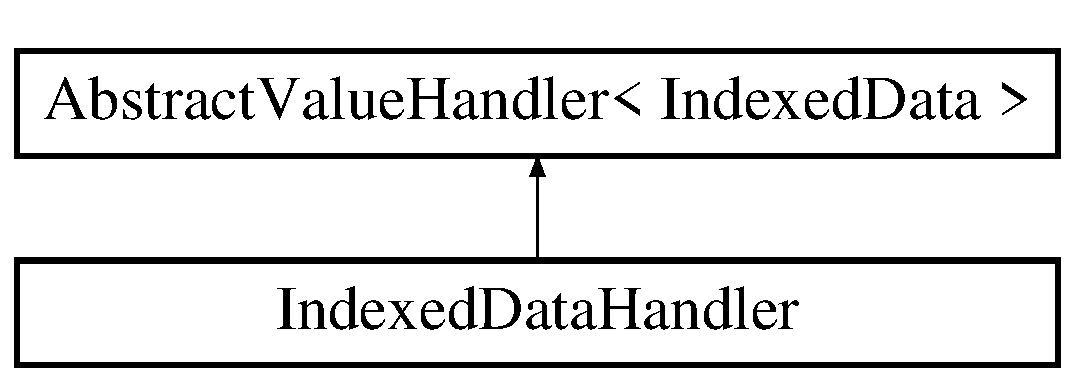
\includegraphics[height=2.000000cm]{classIndexedDataHandler}
\end{center}
\end{figure}
\subsection*{Public Member Functions}
\begin{DoxyCompactItemize}
\item 
virtual std\+::string \hyperlink{classIndexedDataHandler_a858b6661224371858487adf4515a929c}{id} ()
\item 
void \hyperlink{classIndexedDataHandler_ab24da9862e5572a9d6f58e51f62fb5c7}{read} (std\+::istream $\ast$in, \hyperlink{classIndexedData}{Indexed\+Data} \&v)
\item 
void \hyperlink{classIndexedDataHandler_adac292491ac7e7e59d15f0a8a76bfac7}{write} (std\+::ostream $\ast$out, \hyperlink{classIndexedData}{Indexed\+Data} \&value)
\item 
virtual std\+::string \hyperlink{classIndexedDataHandler_a7a3fd16bf83956b3fbc2fe46578aa958}{tostring} (\hyperlink{classIndexedData}{Indexed\+Data} \&value)
\item 
unsigned int \hyperlink{classIndexedDataHandler_a9ce91a864dceb5e7de23ee89d1083037}{count} (\hyperlink{classIndexedData}{Indexed\+Data} \&value) const 
\item 
void \hyperlink{classIndexedDataHandler_a242beac1d0b430238e3259556d2b1426}{add} (\hyperlink{classIndexedData}{Indexed\+Data} $\ast$value, const \hyperlink{classIndexReference}{Index\+Reference} \&ref) const 
\item 
void \hyperlink{classIndexedDataHandler_a5f4e87e6b1d952f9a1724168786bc99e}{convertto} (\hyperlink{classIndexedData}{Indexed\+Data} $\ast$source, \hyperlink{classIndexedData}{Indexed\+Data} $\ast$\&target) const 
\item 
void \hyperlink{classIndexedDataHandler_ab9ceda9fb27c913f8d14c25d714ac461}{convertto} (\hyperlink{classIndexedData}{Indexed\+Data} $\ast$value, unsigned int $\ast$\&convertedvalue) const 
\end{DoxyCompactItemize}
\subsection*{Static Public Attributes}
\begin{DoxyCompactItemize}
\item 
static const bool \hyperlink{classIndexedDataHandler_a08512932e8b482034656d21c67773571}{indexed} = true
\end{DoxyCompactItemize}


\subsection{Detailed Description}
Data handler for \hyperlink{classIndexedData}{Indexed\+Data}. Deals with serialisation from/to file and conversions. 

\subsection{Member Function Documentation}
\hypertarget{classIndexedDataHandler_a242beac1d0b430238e3259556d2b1426}{}\index{Indexed\+Data\+Handler@{Indexed\+Data\+Handler}!add@{add}}
\index{add@{add}!Indexed\+Data\+Handler@{Indexed\+Data\+Handler}}
\subsubsection[{add(\+Indexed\+Data $\ast$value, const Index\+Reference \&ref) const }]{\setlength{\rightskip}{0pt plus 5cm}void Indexed\+Data\+Handler\+::add (
\begin{DoxyParamCaption}
\item[{{\bf Indexed\+Data} $\ast$}]{value, }
\item[{const {\bf Index\+Reference} \&}]{ref}
\end{DoxyParamCaption}
) const\hspace{0.3cm}{\ttfamily [inline]}, {\ttfamily [virtual]}}\label{classIndexedDataHandler_a242beac1d0b430238e3259556d2b1426}


Implements \hyperlink{classAbstractValueHandler_a72ecec2580cb5a9a3ba1495a98d08d98}{Abstract\+Value\+Handler$<$ Indexed\+Data $>$}.

\hypertarget{classIndexedDataHandler_a5f4e87e6b1d952f9a1724168786bc99e}{}\index{Indexed\+Data\+Handler@{Indexed\+Data\+Handler}!convertto@{convertto}}
\index{convertto@{convertto}!Indexed\+Data\+Handler@{Indexed\+Data\+Handler}}
\subsubsection[{convertto(\+Indexed\+Data $\ast$source, Indexed\+Data $\ast$\&target) const }]{\setlength{\rightskip}{0pt plus 5cm}void Indexed\+Data\+Handler\+::convertto (
\begin{DoxyParamCaption}
\item[{{\bf Indexed\+Data} $\ast$}]{source, }
\item[{{\bf Indexed\+Data} $\ast$\&}]{target}
\end{DoxyParamCaption}
) const\hspace{0.3cm}{\ttfamily [inline]}, {\ttfamily [virtual]}}\label{classIndexedDataHandler_a5f4e87e6b1d952f9a1724168786bc99e}


Reimplemented from \hyperlink{classAbstractValueHandler_ae89579ec77805153a0acc617202f89b4}{Abstract\+Value\+Handler$<$ Indexed\+Data $>$}.

\hypertarget{classIndexedDataHandler_ab9ceda9fb27c913f8d14c25d714ac461}{}\index{Indexed\+Data\+Handler@{Indexed\+Data\+Handler}!convertto@{convertto}}
\index{convertto@{convertto}!Indexed\+Data\+Handler@{Indexed\+Data\+Handler}}
\subsubsection[{convertto(\+Indexed\+Data $\ast$value, unsigned int $\ast$\&convertedvalue) const }]{\setlength{\rightskip}{0pt plus 5cm}void Indexed\+Data\+Handler\+::convertto (
\begin{DoxyParamCaption}
\item[{{\bf Indexed\+Data} $\ast$}]{value, }
\item[{unsigned int $\ast$\&}]{convertedvalue}
\end{DoxyParamCaption}
) const\hspace{0.3cm}{\ttfamily [inline]}}\label{classIndexedDataHandler_ab9ceda9fb27c913f8d14c25d714ac461}
\hypertarget{classIndexedDataHandler_a9ce91a864dceb5e7de23ee89d1083037}{}\index{Indexed\+Data\+Handler@{Indexed\+Data\+Handler}!count@{count}}
\index{count@{count}!Indexed\+Data\+Handler@{Indexed\+Data\+Handler}}
\subsubsection[{count(\+Indexed\+Data \&value) const }]{\setlength{\rightskip}{0pt plus 5cm}unsigned int Indexed\+Data\+Handler\+::count (
\begin{DoxyParamCaption}
\item[{{\bf Indexed\+Data} \&}]{value}
\end{DoxyParamCaption}
) const\hspace{0.3cm}{\ttfamily [inline]}, {\ttfamily [virtual]}}\label{classIndexedDataHandler_a9ce91a864dceb5e7de23ee89d1083037}


Implements \hyperlink{classAbstractValueHandler_a1d5941f6ff2afaee0c0bfc89ccb5188e}{Abstract\+Value\+Handler$<$ Indexed\+Data $>$}.

\hypertarget{classIndexedDataHandler_a858b6661224371858487adf4515a929c}{}\index{Indexed\+Data\+Handler@{Indexed\+Data\+Handler}!id@{id}}
\index{id@{id}!Indexed\+Data\+Handler@{Indexed\+Data\+Handler}}
\subsubsection[{id()}]{\setlength{\rightskip}{0pt plus 5cm}virtual std\+::string Indexed\+Data\+Handler\+::id (
\begin{DoxyParamCaption}
{}
\end{DoxyParamCaption}
)\hspace{0.3cm}{\ttfamily [inline]}, {\ttfamily [virtual]}}\label{classIndexedDataHandler_a858b6661224371858487adf4515a929c}


Reimplemented from \hyperlink{classAbstractValueHandler_a6e2f7abe130cdec1062e51d56e4f9fac}{Abstract\+Value\+Handler$<$ Indexed\+Data $>$}.

\hypertarget{classIndexedDataHandler_ab24da9862e5572a9d6f58e51f62fb5c7}{}\index{Indexed\+Data\+Handler@{Indexed\+Data\+Handler}!read@{read}}
\index{read@{read}!Indexed\+Data\+Handler@{Indexed\+Data\+Handler}}
\subsubsection[{read(std\+::istream $\ast$in, Indexed\+Data \&v)}]{\setlength{\rightskip}{0pt plus 5cm}void Indexed\+Data\+Handler\+::read (
\begin{DoxyParamCaption}
\item[{std\+::istream $\ast$}]{in, }
\item[{{\bf Indexed\+Data} \&}]{v}
\end{DoxyParamCaption}
)\hspace{0.3cm}{\ttfamily [inline]}, {\ttfamily [virtual]}}\label{classIndexedDataHandler_ab24da9862e5572a9d6f58e51f62fb5c7}


Implements \hyperlink{classAbstractValueHandler_ac7921fae157361b054e467bf96785654}{Abstract\+Value\+Handler$<$ Indexed\+Data $>$}.

\hypertarget{classIndexedDataHandler_a7a3fd16bf83956b3fbc2fe46578aa958}{}\index{Indexed\+Data\+Handler@{Indexed\+Data\+Handler}!tostring@{tostring}}
\index{tostring@{tostring}!Indexed\+Data\+Handler@{Indexed\+Data\+Handler}}
\subsubsection[{tostring(\+Indexed\+Data \&value)}]{\setlength{\rightskip}{0pt plus 5cm}virtual std\+::string Indexed\+Data\+Handler\+::tostring (
\begin{DoxyParamCaption}
\item[{{\bf Indexed\+Data} \&}]{value}
\end{DoxyParamCaption}
)\hspace{0.3cm}{\ttfamily [inline]}, {\ttfamily [virtual]}}\label{classIndexedDataHandler_a7a3fd16bf83956b3fbc2fe46578aa958}


Implements \hyperlink{classAbstractValueHandler_a8e56e3bbccc464a47a666352249e6a1b}{Abstract\+Value\+Handler$<$ Indexed\+Data $>$}.

\hypertarget{classIndexedDataHandler_adac292491ac7e7e59d15f0a8a76bfac7}{}\index{Indexed\+Data\+Handler@{Indexed\+Data\+Handler}!write@{write}}
\index{write@{write}!Indexed\+Data\+Handler@{Indexed\+Data\+Handler}}
\subsubsection[{write(std\+::ostream $\ast$out, Indexed\+Data \&value)}]{\setlength{\rightskip}{0pt plus 5cm}void Indexed\+Data\+Handler\+::write (
\begin{DoxyParamCaption}
\item[{std\+::ostream $\ast$}]{out, }
\item[{{\bf Indexed\+Data} \&}]{value}
\end{DoxyParamCaption}
)\hspace{0.3cm}{\ttfamily [inline]}, {\ttfamily [virtual]}}\label{classIndexedDataHandler_adac292491ac7e7e59d15f0a8a76bfac7}


Implements \hyperlink{classAbstractValueHandler_aecd2820bc132f8065babbec5cd7458b8}{Abstract\+Value\+Handler$<$ Indexed\+Data $>$}.



\subsection{Member Data Documentation}
\hypertarget{classIndexedDataHandler_a08512932e8b482034656d21c67773571}{}\index{Indexed\+Data\+Handler@{Indexed\+Data\+Handler}!indexed@{indexed}}
\index{indexed@{indexed}!Indexed\+Data\+Handler@{Indexed\+Data\+Handler}}
\subsubsection[{indexed}]{\setlength{\rightskip}{0pt plus 5cm}const bool Indexed\+Data\+Handler\+::indexed = true\hspace{0.3cm}{\ttfamily [static]}}\label{classIndexedDataHandler_a08512932e8b482034656d21c67773571}


The documentation for this class was generated from the following file\+:\begin{DoxyCompactItemize}
\item 
include/\hyperlink{datatypes_8h}{datatypes.\+h}\end{DoxyCompactItemize}

\hypertarget{classIndexedPatternModel}{}\section{Indexed\+Pattern\+Model$<$ Map\+Type $>$ Class Template Reference}
\label{classIndexedPatternModel}\index{Indexed\+Pattern\+Model$<$ Map\+Type $>$@{Indexed\+Pattern\+Model$<$ Map\+Type $>$}}


An indexed model mapping patterns to values, high-\/level interface. This is a specialised subclass of \hyperlink{classPatternMap}{Pattern\+Map}.  




{\ttfamily \#include $<$patternmodel.\+h$>$}

Inheritance diagram for Indexed\+Pattern\+Model$<$ Map\+Type $>$\+:\begin{figure}[H]
\begin{center}
\leavevmode
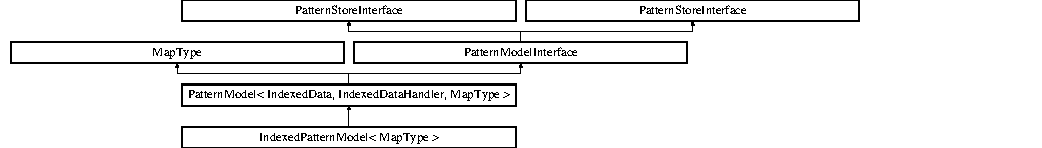
\includegraphics[height=1.991111cm]{classIndexedPatternModel}
\end{center}
\end{figure}
\subsection*{Public Member Functions}
\begin{DoxyCompactItemize}
\item 
void \hyperlink{classIndexedPatternModel_a0d53765f0498911c976744cc3670ff72}{buildreverseindex} (const \hyperlink{classPatternModelOptions}{Pattern\+Model\+Options} options)
\item 
\hyperlink{classIndexedPatternModel_af2fbb7d1f40210bda30bee3d5577546a}{Indexed\+Pattern\+Model} (\hyperlink{classIndexedCorpus}{Indexed\+Corpus} $\ast$corpus=N\+U\+L\+L)
\item 
\hyperlink{classIndexedPatternModel_a983367ac09e96735a2075a1f780d1de4}{Indexed\+Pattern\+Model} (std\+::istream $\ast$f, const \hyperlink{classPatternModelOptions}{Pattern\+Model\+Options} options, \hyperlink{classPatternModelInterface}{Pattern\+Model\+Interface} $\ast$constrainmodel=N\+U\+L\+L, \hyperlink{classIndexedCorpus}{Indexed\+Corpus} $\ast$corpus=N\+U\+L\+L)
\item 
\hyperlink{classIndexedPatternModel_a8d49b0f8aea957fc80e7e8d7b4dd5ba8}{Indexed\+Pattern\+Model} (const std\+::string filename, const \hyperlink{classPatternModelOptions}{Pattern\+Model\+Options} options, \hyperlink{classPatternModelInterface}{Pattern\+Model\+Interface} $\ast$constrainmodel=N\+U\+L\+L, \hyperlink{classIndexedCorpus}{Indexed\+Corpus} $\ast$corpus=N\+U\+L\+L)
\item 
virtual \hyperlink{classIndexedPatternModel_aadc89a95b7ef0874ab5d763d0c453e79}{$\sim$\+Indexed\+Pattern\+Model} ()
\item 
int \hyperlink{classIndexedPatternModel_adeb6b2bce5dc4fcdd9f8ec9f723d0f5b}{getmodeltype} () const 
\item 
int \hyperlink{classIndexedPatternModel_adabaad88e64edd1c4762a56c86d1bae4}{getmodelversion} () const 
\item 
void \hyperlink{classIndexedPatternModel_a41367fc32c9fa72d1a88e60d749015a5}{add} (const \hyperlink{classPattern}{Pattern} \&pattern, \hyperlink{classIndexedData}{Indexed\+Data} $\ast$value, const \hyperlink{classIndexReference}{Index\+Reference} \&ref)
\item 
void \hyperlink{classIndexedPatternModel_a83e3a00515a9ad419b4a2f820278c5f7}{add} (const \hyperlink{classPatternPointer}{Pattern\+Pointer} \&patternpointer, \hyperlink{classIndexedData}{Indexed\+Data} $\ast$value, const \hyperlink{classIndexReference}{Index\+Reference} \&ref)
\item 
\hyperlink{classIndexedData}{Indexed\+Data} $\ast$ \hyperlink{classIndexedPatternModel_a1ee41056c7235bf03573e6532cd5efce}{getdata} (const \hyperlink{classPattern}{Pattern} \&pattern, bool makeifnew=false)
\item 
\hyperlink{classIndexedData}{Indexed\+Data} $\ast$ \hyperlink{classIndexedPatternModel_a9311529a1123f602720b9e95f3f89236}{getdata} (const \hyperlink{classPatternPointer}{Pattern\+Pointer} \&patternpointer, bool makeifnew=false)
\item 
void \hyperlink{classIndexedPatternModel_a64fade10459a7699b856c8cb621789f9}{info} (std\+::ostream $\ast$O\+U\+T)
\item 
void \hyperlink{classIndexedPatternModel_a4a5f41aa99e3b93a9a816e9c21b9b790}{print} (std\+::ostream $\ast$out, \hyperlink{classClassDecoder}{Class\+Decoder} \&decoder)
\item 
void \hyperlink{classIndexedPatternModel_aed4218c952b051b523d8d5a31c5c00fb}{print} (std\+::ostream $\ast$out, \hyperlink{classClassDecoder}{Class\+Decoder} \&decoder, const \hyperlink{classPattern}{Pattern} \&pattern, bool endline=true)
\item 
virtual void \hyperlink{classIndexedPatternModel_acf0b5ec19f8b76b875dbef07ca0cb398}{trainskipgrams} (\hyperlink{classPatternModelOptions}{Pattern\+Model\+Options} options, \hyperlink{classPatternModelInterface}{Pattern\+Model\+Interface} $\ast$constrainbymodel=N\+U\+L\+L)
\item 
\hyperlink{classPattern}{Pattern} \hyperlink{classIndexedPatternModel_a205e5f3a0019a9948064084c0b92a7ce}{getpatternfromtoken} (\hyperlink{classIndexReference}{Index\+Reference} ref)
\item 
\hyperlink{patternmodel_8h_a8695a2b10be5a74c827cd6c11bd46fb9}{t\+\_\+relationmap} \hyperlink{classIndexedPatternModel_ac2478fc9fd1eabfc616c1692fc2a58d9}{getskipcontent} (const \hyperlink{classPattern}{Pattern} \&pattern)
\item 
void \hyperlink{classIndexedPatternModel_a0509989bf6bcb7d09dbc0e5c9e3dc84a}{prunerelations} (\hyperlink{patternmodel_8h_a8695a2b10be5a74c827cd6c11bd46fb9}{t\+\_\+relationmap} \&relations, unsigned int occurrencethreshold)
\item 
\hyperlink{patternmodel_8h_a8695a2b10be5a74c827cd6c11bd46fb9}{t\+\_\+relationmap} \hyperlink{classIndexedPatternModel_a951ae48d5f211af94a3c63102f708356}{gettemplates} (const \hyperlink{classPattern}{Pattern} \&pattern, unsigned int occurrencethreshold=0)
\item 
\hyperlink{patternmodel_8h_a8695a2b10be5a74c827cd6c11bd46fb9}{t\+\_\+relationmap} \hyperlink{classIndexedPatternModel_a2942d0920ce1e646cb733c0c84fdd0d7}{getinstances} (const \hyperlink{classPattern}{Pattern} \&pattern, unsigned int occurrencethreshold=0)
\item 
\hyperlink{patternmodel_8h_a8695a2b10be5a74c827cd6c11bd46fb9}{t\+\_\+relationmap} \hyperlink{classIndexedPatternModel_a785f4b6ef4229843b90ba895957a1b56}{getsubchildren} (const \hyperlink{classPattern}{Pattern} \&pattern, unsigned int occurrencethreshold=0, int category=0, unsigned int \hyperlink{classPatternModel_a25f387acaf981af9962195bd05b3e7e2}{size}=0)
\item 
\hyperlink{patternmodel_8h_a8695a2b10be5a74c827cd6c11bd46fb9}{t\+\_\+relationmap} \hyperlink{classIndexedPatternModel_aed2ec73f5bece8595e6f6ab4f180ce75}{getsubparents} (const \hyperlink{classPattern}{Pattern} \&pattern, unsigned int occurrencethreshold=0, int category=0, unsigned int \hyperlink{classPatternModel_a25f387acaf981af9962195bd05b3e7e2}{size}=0)
\item 
\hyperlink{patternmodel_8h_a8695a2b10be5a74c827cd6c11bd46fb9}{t\+\_\+relationmap} \hyperlink{classIndexedPatternModel_a7d3909fc9e28191fa2f47be30b3dd99e}{getleftneighbours} (const \hyperlink{classPattern}{Pattern} \&pattern, unsigned int occurrencethreshold=0, int category=0, unsigned int \hyperlink{classPatternModel_a25f387acaf981af9962195bd05b3e7e2}{size}=0, unsigned int cutoff=0)
\item 
\hyperlink{patternmodel_8h_a8695a2b10be5a74c827cd6c11bd46fb9}{t\+\_\+relationmap} \hyperlink{classIndexedPatternModel_ab2d837b1f82f65b18ab6a7fc3ba2b15c}{getrightneighbours} (const \hyperlink{classPattern}{Pattern} \&pattern, unsigned int occurrencethreshold=0, int category=0, unsigned int \hyperlink{classPatternModel_a25f387acaf981af9962195bd05b3e7e2}{size}=0, unsigned int cutoff=0)
\item 
int \hyperlink{classIndexedPatternModel_a0df4f0e3a55dd00c0fe00fc3841f66ed}{pruneskipgrams} (int threshold, int minskiptypes, int \+\_\+n=0)
\item 
virtual void \hyperlink{classIndexedPatternModel_acf70c3536f4869b3e8330289f7409bf5}{computecoveragestats} ()
\item 
\hyperlink{patternmodel_8h_a8695a2b10be5a74c827cd6c11bd46fb9}{t\+\_\+relationmap} \hyperlink{classIndexedPatternModel_ad0d8258d41c372a17b91f8be08f3f305}{getrightcooc} (const \hyperlink{classPattern}{Pattern} \&pattern, unsigned int occurrencethreshold=0, int category=0, unsigned int \hyperlink{classPatternModel_a25f387acaf981af9962195bd05b3e7e2}{size}=0, \hyperlink{classIndexedData}{Indexed\+Data} $\ast$matches=N\+U\+L\+L)
\item 
\hyperlink{patternmodel_8h_a8695a2b10be5a74c827cd6c11bd46fb9}{t\+\_\+relationmap} \hyperlink{classIndexedPatternModel_a9f9292a132bac92267f26eeae00fd8ee}{getleftcooc} (const \hyperlink{classPattern}{Pattern} \&pattern, unsigned int occurrencethreshold=0, int category=0, unsigned int \hyperlink{classPatternModel_a25f387acaf981af9962195bd05b3e7e2}{size}=0)
\item 
\hyperlink{patternmodel_8h_a8695a2b10be5a74c827cd6c11bd46fb9}{t\+\_\+relationmap} \hyperlink{classIndexedPatternModel_aaa6caa3a7aa9ce15087b98dd8d2b1c4b}{getcooc} (const \hyperlink{classPattern}{Pattern} \&pattern, unsigned int occurrencethreshold=0, int category=0, unsigned int \hyperlink{classPatternModel_a25f387acaf981af9962195bd05b3e7e2}{size}=0, bool ordersignificant=false)
\item 
double \hyperlink{classIndexedPatternModel_a03c138c720ca2724457f2786626478d3}{npmi} (const \hyperlink{classPattern}{Pattern} \&key1, const \hyperlink{classPattern}{Pattern} \&key2, int jointcount)
\item 
void \hyperlink{classIndexedPatternModel_a001c634d095eee8883e8cd8fd24846d8}{outputrelations} (const \hyperlink{classPattern}{Pattern} \&pattern, \hyperlink{patternmodel_8h_a8695a2b10be5a74c827cd6c11bd46fb9}{t\+\_\+relationmap} \&relations, \hyperlink{classClassDecoder}{Class\+Decoder} \&classdecoder, std\+::ostream $\ast$O\+U\+T, const std\+::string label=\char`\"{}R\+E\+L\+A\+T\+E\+D-\/T\+O\char`\"{})
\item 
void \hyperlink{classIndexedPatternModel_abfe968ebfe686a774ae70c810d2d9cc3}{outputrelations} (const \hyperlink{classPattern}{Pattern} \&pattern, \hyperlink{classClassDecoder}{Class\+Decoder} \&classdecoder, std\+::ostream $\ast$O\+U\+T, bool outputheader=true)
\item 
void \hyperlink{classIndexedPatternModel_ab07346735ccdee4d7e42043e95d1bc2e}{computenpmi} (std\+::map$<$ \hyperlink{classPattern}{Pattern}, \hyperlink{patternmodel_8h_ae13b52c8cf777358f19da17c90c7dac0}{t\+\_\+relationmap\+\_\+double} $>$ \&coocmap, double threshold, bool right=true, bool left=true)
\item 
void \hyperlink{classIndexedPatternModel_ae62d20c9507dee1edd2f133cf3de2a5f}{computecooc} (std\+::map$<$ \hyperlink{classPattern}{Pattern}, \hyperlink{patternmodel_8h_a8695a2b10be5a74c827cd6c11bd46fb9}{t\+\_\+relationmap} $>$ \&coocmap, int threshold, bool right=true, bool left=true)
\item 
int \hyperlink{classIndexedPatternModel_ad3b8e1405429aa869501f9117664b0d5}{computeflexgrams\+\_\+fromskipgrams} ()
\item 
int \hyperlink{classIndexedPatternModel_a2d1a24a490466115aad4cf09058337ec}{computeflexgrams\+\_\+fromcooc} (double threshold)
\item 
void \hyperlink{classIndexedPatternModel_a4e8d1bf4017173e8214cfd37bab576c1}{outputcooc\+\_\+npmi} (std\+::ostream $\ast$O\+U\+T, \hyperlink{classClassDecoder}{Class\+Decoder} \&classdecoder, double threshold)
\item 
void \hyperlink{classIndexedPatternModel_a6ab1e2d6bf0a8aeed25a39c306e51c34}{outputcooc} (std\+::ostream $\ast$O\+U\+T, \hyperlink{classClassDecoder}{Class\+Decoder} \&classdecoder, double threshold)
\item 
int \hyperlink{classIndexedPatternModel_abd312da331baffd69a7944084cc0e4f6}{flexgramsize} (const \hyperlink{classPattern}{Pattern} \&pattern, \hyperlink{classIndexReference}{Index\+Reference} begin)
\end{DoxyCompactItemize}
\subsection*{Protected Member Functions}
\begin{DoxyCompactItemize}
\item 
virtual void \hyperlink{classIndexedPatternModel_a82f5f4fffea239a4f5bde4d346691f5d}{postread} (const \hyperlink{classPatternModelOptions}{Pattern\+Model\+Options} options)
\item 
virtual void \hyperlink{classIndexedPatternModel_a4a39df881afb2ef2c6c4a29afe9aa6ff}{posttrain} (const \hyperlink{classPatternModelOptions}{Pattern\+Model\+Options} options)
\end{DoxyCompactItemize}
\subsection*{Additional Inherited Members}


\subsection{Detailed Description}
\subsubsection*{template$<$class Map\+Type = Pattern\+Map$<$\+Indexed\+Data,\+Indexed\+Data\+Handler$>$$>$class Indexed\+Pattern\+Model$<$ Map\+Type $>$}

An indexed model mapping patterns to values, high-\/level interface. This is a specialised subclass of \hyperlink{classPatternMap}{Pattern\+Map}. 


\begin{DoxyTemplParams}{Template Parameters}
{\em Map\+Type} & The type of container to use \\
\hline
\end{DoxyTemplParams}


\subsection{Constructor \& Destructor Documentation}
\hypertarget{classIndexedPatternModel_af2fbb7d1f40210bda30bee3d5577546a}{}\index{Indexed\+Pattern\+Model@{Indexed\+Pattern\+Model}!Indexed\+Pattern\+Model@{Indexed\+Pattern\+Model}}
\index{Indexed\+Pattern\+Model@{Indexed\+Pattern\+Model}!Indexed\+Pattern\+Model@{Indexed\+Pattern\+Model}}
\subsubsection[{Indexed\+Pattern\+Model(\+Indexed\+Corpus $\ast$corpus=\+N\+U\+L\+L)}]{\setlength{\rightskip}{0pt plus 5cm}template$<$class Map\+Type = Pattern\+Map$<$\+Indexed\+Data,\+Indexed\+Data\+Handler$>$$>$ {\bf Indexed\+Pattern\+Model}$<$ Map\+Type $>$\+::{\bf Indexed\+Pattern\+Model} (
\begin{DoxyParamCaption}
\item[{{\bf Indexed\+Corpus} $\ast$}]{corpus = {\ttfamily NULL}}
\end{DoxyParamCaption}
)\hspace{0.3cm}{\ttfamily [inline]}}\label{classIndexedPatternModel_af2fbb7d1f40210bda30bee3d5577546a}
Begin a new pattern model, optionally pre-\/setting a reverseindex. \hypertarget{classIndexedPatternModel_a983367ac09e96735a2075a1f780d1de4}{}\index{Indexed\+Pattern\+Model@{Indexed\+Pattern\+Model}!Indexed\+Pattern\+Model@{Indexed\+Pattern\+Model}}
\index{Indexed\+Pattern\+Model@{Indexed\+Pattern\+Model}!Indexed\+Pattern\+Model@{Indexed\+Pattern\+Model}}
\subsubsection[{Indexed\+Pattern\+Model(std\+::istream $\ast$f, const Pattern\+Model\+Options options, Pattern\+Model\+Interface $\ast$constrainmodel=\+N\+U\+L\+L, Indexed\+Corpus $\ast$corpus=\+N\+U\+L\+L)}]{\setlength{\rightskip}{0pt plus 5cm}template$<$class Map\+Type = Pattern\+Map$<$\+Indexed\+Data,\+Indexed\+Data\+Handler$>$$>$ {\bf Indexed\+Pattern\+Model}$<$ Map\+Type $>$\+::{\bf Indexed\+Pattern\+Model} (
\begin{DoxyParamCaption}
\item[{std\+::istream $\ast$}]{f, }
\item[{const {\bf Pattern\+Model\+Options}}]{options, }
\item[{{\bf Pattern\+Model\+Interface} $\ast$}]{constrainmodel = {\ttfamily NULL}, }
\item[{{\bf Indexed\+Corpus} $\ast$}]{corpus = {\ttfamily NULL}}
\end{DoxyParamCaption}
)\hspace{0.3cm}{\ttfamily [inline]}}\label{classIndexedPatternModel_a983367ac09e96735a2075a1f780d1de4}
Read a pattern model from an input stream 
\begin{DoxyParams}{Parameters}
{\em f} & The input stream \\
\hline
{\em options} & Options for reading, these act as filter for the data, allowing you to raise thresholds etc \\
\hline
{\em constrainmodel} & Pointer to another pattern model which should be used to constrain the loading of this one, only patterns also occurring in the other model will be included. Defaults to N\+U\+L\+L (no constraining) \\
\hline
{\em corpus} & Pointer to the loaded corpus, used as a reverse index. \\
\hline
\end{DoxyParams}
\hypertarget{classIndexedPatternModel_a8d49b0f8aea957fc80e7e8d7b4dd5ba8}{}\index{Indexed\+Pattern\+Model@{Indexed\+Pattern\+Model}!Indexed\+Pattern\+Model@{Indexed\+Pattern\+Model}}
\index{Indexed\+Pattern\+Model@{Indexed\+Pattern\+Model}!Indexed\+Pattern\+Model@{Indexed\+Pattern\+Model}}
\subsubsection[{Indexed\+Pattern\+Model(const std\+::string filename, const Pattern\+Model\+Options options, Pattern\+Model\+Interface $\ast$constrainmodel=\+N\+U\+L\+L, Indexed\+Corpus $\ast$corpus=\+N\+U\+L\+L)}]{\setlength{\rightskip}{0pt plus 5cm}template$<$class Map\+Type = Pattern\+Map$<$\+Indexed\+Data,\+Indexed\+Data\+Handler$>$$>$ {\bf Indexed\+Pattern\+Model}$<$ Map\+Type $>$\+::{\bf Indexed\+Pattern\+Model} (
\begin{DoxyParamCaption}
\item[{const std\+::string}]{filename, }
\item[{const {\bf Pattern\+Model\+Options}}]{options, }
\item[{{\bf Pattern\+Model\+Interface} $\ast$}]{constrainmodel = {\ttfamily NULL}, }
\item[{{\bf Indexed\+Corpus} $\ast$}]{corpus = {\ttfamily NULL}}
\end{DoxyParamCaption}
)\hspace{0.3cm}{\ttfamily [inline]}}\label{classIndexedPatternModel_a8d49b0f8aea957fc80e7e8d7b4dd5ba8}
Read a pattern model from file 
\begin{DoxyParams}{Parameters}
{\em filename} & The filename \\
\hline
{\em options} & Options for reading, these act as filter for the data, allowing you to raise thresholds etc \\
\hline
{\em constrainmodel} & Pointer to another pattern model which should be used to constrain the loading of this one, only patterns also occurring in the other model will be included. Defaults to N\+U\+L\+L (no constraining) \\
\hline
{\em corpus} & Pointer to the loaded corpus, used as a reverse index. \\
\hline
\end{DoxyParams}
\hypertarget{classIndexedPatternModel_aadc89a95b7ef0874ab5d763d0c453e79}{}\index{Indexed\+Pattern\+Model@{Indexed\+Pattern\+Model}!````~Indexed\+Pattern\+Model@{$\sim$\+Indexed\+Pattern\+Model}}
\index{````~Indexed\+Pattern\+Model@{$\sim$\+Indexed\+Pattern\+Model}!Indexed\+Pattern\+Model@{Indexed\+Pattern\+Model}}
\subsubsection[{$\sim$\+Indexed\+Pattern\+Model()}]{\setlength{\rightskip}{0pt plus 5cm}template$<$class Map\+Type = Pattern\+Map$<$\+Indexed\+Data,\+Indexed\+Data\+Handler$>$$>$ virtual {\bf Indexed\+Pattern\+Model}$<$ Map\+Type $>$\+::$\sim${\bf Indexed\+Pattern\+Model} (
\begin{DoxyParamCaption}
{}
\end{DoxyParamCaption}
)\hspace{0.3cm}{\ttfamily [inline]}, {\ttfamily [virtual]}}\label{classIndexedPatternModel_aadc89a95b7ef0874ab5d763d0c453e79}


\subsection{Member Function Documentation}
\hypertarget{classIndexedPatternModel_a41367fc32c9fa72d1a88e60d749015a5}{}\index{Indexed\+Pattern\+Model@{Indexed\+Pattern\+Model}!add@{add}}
\index{add@{add}!Indexed\+Pattern\+Model@{Indexed\+Pattern\+Model}}
\subsubsection[{add(const Pattern \&pattern, Indexed\+Data $\ast$value, const Index\+Reference \&ref)}]{\setlength{\rightskip}{0pt plus 5cm}template$<$class Map\+Type = Pattern\+Map$<$\+Indexed\+Data,\+Indexed\+Data\+Handler$>$$>$ void {\bf Indexed\+Pattern\+Model}$<$ Map\+Type $>$\+::add (
\begin{DoxyParamCaption}
\item[{const {\bf Pattern} \&}]{pattern, }
\item[{{\bf Indexed\+Data} $\ast$}]{value, }
\item[{const {\bf Index\+Reference} \&}]{ref}
\end{DoxyParamCaption}
)\hspace{0.3cm}{\ttfamily [inline]}, {\ttfamily [virtual]}}\label{classIndexedPatternModel_a41367fc32c9fa72d1a88e60d749015a5}
Add a pattern, with a given position, and a value to the model. This is called during training at every time an instance of a pattern is found in the data. 
\begin{DoxyParams}{Parameters}
{\em pattern} & The pattern to add \\
\hline
{\em value} & A pointer to the value for this pattern, set to N\+U\+L\+L and it will be automatically determined \\
\hline
{\em \hyperlink{classIndexReference}{Index\+Reference}} & The position in the corpus where the patterns occurs \\
\hline
\end{DoxyParams}


Reimplemented from \hyperlink{classPatternModel_a0cdb8badafbce0f56089f7c2b8f4716a}{Pattern\+Model$<$ Indexed\+Data, Indexed\+Data\+Handler, Map\+Type $>$}.

\hypertarget{classIndexedPatternModel_a83e3a00515a9ad419b4a2f820278c5f7}{}\index{Indexed\+Pattern\+Model@{Indexed\+Pattern\+Model}!add@{add}}
\index{add@{add}!Indexed\+Pattern\+Model@{Indexed\+Pattern\+Model}}
\subsubsection[{add(const Pattern\+Pointer \&patternpointer, Indexed\+Data $\ast$value, const Index\+Reference \&ref)}]{\setlength{\rightskip}{0pt plus 5cm}template$<$class Map\+Type = Pattern\+Map$<$\+Indexed\+Data,\+Indexed\+Data\+Handler$>$$>$ void {\bf Indexed\+Pattern\+Model}$<$ Map\+Type $>$\+::add (
\begin{DoxyParamCaption}
\item[{const {\bf Pattern\+Pointer} \&}]{patternpointer, }
\item[{{\bf Indexed\+Data} $\ast$}]{value, }
\item[{const {\bf Index\+Reference} \&}]{ref}
\end{DoxyParamCaption}
)\hspace{0.3cm}{\ttfamily [inline]}, {\ttfamily [virtual]}}\label{classIndexedPatternModel_a83e3a00515a9ad419b4a2f820278c5f7}


Reimplemented from \hyperlink{classPatternModel_ad16097db7894d75815cd40ef5acc99a5}{Pattern\+Model$<$ Indexed\+Data, Indexed\+Data\+Handler, Map\+Type $>$}.

\hypertarget{classIndexedPatternModel_a0d53765f0498911c976744cc3670ff72}{}\index{Indexed\+Pattern\+Model@{Indexed\+Pattern\+Model}!buildreverseindex@{buildreverseindex}}
\index{buildreverseindex@{buildreverseindex}!Indexed\+Pattern\+Model@{Indexed\+Pattern\+Model}}
\subsubsection[{buildreverseindex(const Pattern\+Model\+Options options)}]{\setlength{\rightskip}{0pt plus 5cm}template$<$class Map\+Type = Pattern\+Map$<$\+Indexed\+Data,\+Indexed\+Data\+Handler$>$$>$ void {\bf Indexed\+Pattern\+Model}$<$ Map\+Type $>$\+::buildreverseindex (
\begin{DoxyParamCaption}
\item[{const {\bf Pattern\+Model\+Options}}]{options}
\end{DoxyParamCaption}
)\hspace{0.3cm}{\ttfamily [inline]}}\label{classIndexedPatternModel_a0d53765f0498911c976744cc3670ff72}
build reverse index, requires options.\+D\+O\+R\+E\+V\+E\+R\+S\+E\+I\+N\+D\+E\+X to be set or won\textquotesingle{}t do anything. Also won\textquotesingle{}t build a reverse index if one is loaded already. Note that pre-\/loading a reverse index when loading/training your model is generally quicker. \hypertarget{classIndexedPatternModel_ae62d20c9507dee1edd2f133cf3de2a5f}{}\index{Indexed\+Pattern\+Model@{Indexed\+Pattern\+Model}!computecooc@{computecooc}}
\index{computecooc@{computecooc}!Indexed\+Pattern\+Model@{Indexed\+Pattern\+Model}}
\subsubsection[{computecooc(std\+::map$<$ Pattern, t\+\_\+relationmap $>$ \&coocmap, int threshold, bool right=true, bool left=true)}]{\setlength{\rightskip}{0pt plus 5cm}template$<$class Map\+Type = Pattern\+Map$<$\+Indexed\+Data,\+Indexed\+Data\+Handler$>$$>$ void {\bf Indexed\+Pattern\+Model}$<$ Map\+Type $>$\+::computecooc (
\begin{DoxyParamCaption}
\item[{std\+::map$<$ {\bf Pattern}, {\bf t\+\_\+relationmap} $>$ \&}]{coocmap, }
\item[{int}]{threshold, }
\item[{bool}]{right = {\ttfamily true}, }
\item[{bool}]{left = {\ttfamily true}}
\end{DoxyParamCaption}
)\hspace{0.3cm}{\ttfamily [inline]}}\label{classIndexedPatternModel_ae62d20c9507dee1edd2f133cf3de2a5f}
Compute co-\/occurence as absolute joint occurrence count, for all patterns 
\begin{DoxyParams}{Parameters}
{\em coocmap} & The map that will store the results \\
\hline
{\em threshold} & Only include pairs passing this N\+P\+M\+I threshold \\
\hline
{\em right} & Compute co-\/occurence to the right (default\+: true) \\
\hline
{\em left} & Compute co-\/occurence to the left (default\+: true) \\
\hline
\end{DoxyParams}
\hypertarget{classIndexedPatternModel_acf70c3536f4869b3e8330289f7409bf5}{}\index{Indexed\+Pattern\+Model@{Indexed\+Pattern\+Model}!computecoveragestats@{computecoveragestats}}
\index{computecoveragestats@{computecoveragestats}!Indexed\+Pattern\+Model@{Indexed\+Pattern\+Model}}
\subsubsection[{computecoveragestats()}]{\setlength{\rightskip}{0pt plus 5cm}template$<$class Map\+Type = Pattern\+Map$<$\+Indexed\+Data,\+Indexed\+Data\+Handler$>$$>$ virtual void {\bf Indexed\+Pattern\+Model}$<$ Map\+Type $>$\+::computecoveragestats (
\begin{DoxyParamCaption}
{}
\end{DoxyParamCaption}
)\hspace{0.3cm}{\ttfamily [inline]}, {\ttfamily [virtual]}}\label{classIndexedPatternModel_acf70c3536f4869b3e8330289f7409bf5}
Compute coverage statistics on the model, will generally be called automatically by methods who use it, and the statistics are cached after computation. 

Reimplemented from \hyperlink{classPatternModel_ae36bb1e641f954ee78a5fbab98ae069a}{Pattern\+Model$<$ Indexed\+Data, Indexed\+Data\+Handler, Map\+Type $>$}.

\hypertarget{classIndexedPatternModel_a2d1a24a490466115aad4cf09058337ec}{}\index{Indexed\+Pattern\+Model@{Indexed\+Pattern\+Model}!computeflexgrams\+\_\+fromcooc@{computeflexgrams\+\_\+fromcooc}}
\index{computeflexgrams\+\_\+fromcooc@{computeflexgrams\+\_\+fromcooc}!Indexed\+Pattern\+Model@{Indexed\+Pattern\+Model}}
\subsubsection[{computeflexgrams\+\_\+fromcooc(double threshold)}]{\setlength{\rightskip}{0pt plus 5cm}template$<$class Map\+Type = Pattern\+Map$<$\+Indexed\+Data,\+Indexed\+Data\+Handler$>$$>$ int {\bf Indexed\+Pattern\+Model}$<$ Map\+Type $>$\+::computeflexgrams\+\_\+fromcooc (
\begin{DoxyParamCaption}
\item[{double}]{threshold}
\end{DoxyParamCaption}
)\hspace{0.3cm}{\ttfamily [inline]}}\label{classIndexedPatternModel_a2d1a24a490466115aad4cf09058337ec}
Compute flexgrams using co-\/occurrence 
\begin{DoxyParams}{Parameters}
{\em threshold} & Normalised Pointwise Mutual Information threshold \\
\hline
\end{DoxyParams}
\begin{DoxyReturn}{Returns}
The number of flexgrams found 
\end{DoxyReturn}
\hypertarget{classIndexedPatternModel_ad3b8e1405429aa869501f9117664b0d5}{}\index{Indexed\+Pattern\+Model@{Indexed\+Pattern\+Model}!computeflexgrams\+\_\+fromskipgrams@{computeflexgrams\+\_\+fromskipgrams}}
\index{computeflexgrams\+\_\+fromskipgrams@{computeflexgrams\+\_\+fromskipgrams}!Indexed\+Pattern\+Model@{Indexed\+Pattern\+Model}}
\subsubsection[{computeflexgrams\+\_\+fromskipgrams()}]{\setlength{\rightskip}{0pt plus 5cm}template$<$class Map\+Type = Pattern\+Map$<$\+Indexed\+Data,\+Indexed\+Data\+Handler$>$$>$ int {\bf Indexed\+Pattern\+Model}$<$ Map\+Type $>$\+::computeflexgrams\+\_\+fromskipgrams (
\begin{DoxyParamCaption}
{}
\end{DoxyParamCaption}
)\hspace{0.3cm}{\ttfamily [inline]}, {\ttfamily [virtual]}}\label{classIndexedPatternModel_ad3b8e1405429aa869501f9117664b0d5}
Compute flexgrams by abstracting from existing skipgrams in the model \begin{DoxyReturn}{Returns}
The number of flexgrams found 
\end{DoxyReturn}


Reimplemented from \hyperlink{classPatternModel_ab393fff93aae08db7456a9e60296a0b3}{Pattern\+Model$<$ Indexed\+Data, Indexed\+Data\+Handler, Map\+Type $>$}.

\hypertarget{classIndexedPatternModel_ab07346735ccdee4d7e42043e95d1bc2e}{}\index{Indexed\+Pattern\+Model@{Indexed\+Pattern\+Model}!computenpmi@{computenpmi}}
\index{computenpmi@{computenpmi}!Indexed\+Pattern\+Model@{Indexed\+Pattern\+Model}}
\subsubsection[{computenpmi(std\+::map$<$ Pattern, t\+\_\+relationmap\+\_\+double $>$ \&coocmap, double threshold, bool right=true, bool left=true)}]{\setlength{\rightskip}{0pt plus 5cm}template$<$class Map\+Type = Pattern\+Map$<$\+Indexed\+Data,\+Indexed\+Data\+Handler$>$$>$ void {\bf Indexed\+Pattern\+Model}$<$ Map\+Type $>$\+::computenpmi (
\begin{DoxyParamCaption}
\item[{std\+::map$<$ {\bf Pattern}, {\bf t\+\_\+relationmap\+\_\+double} $>$ \&}]{coocmap, }
\item[{double}]{threshold, }
\item[{bool}]{right = {\ttfamily true}, }
\item[{bool}]{left = {\ttfamily true}}
\end{DoxyParamCaption}
)\hspace{0.3cm}{\ttfamily [inline]}}\label{classIndexedPatternModel_ab07346735ccdee4d7e42043e95d1bc2e}
\hypertarget{classIndexedPatternModel_abd312da331baffd69a7944084cc0e4f6}{}\index{Indexed\+Pattern\+Model@{Indexed\+Pattern\+Model}!flexgramsize@{flexgramsize}}
\index{flexgramsize@{flexgramsize}!Indexed\+Pattern\+Model@{Indexed\+Pattern\+Model}}
\subsubsection[{flexgramsize(const Pattern \&pattern, Index\+Reference begin)}]{\setlength{\rightskip}{0pt plus 5cm}template$<$class Map\+Type = Pattern\+Map$<$\+Indexed\+Data,\+Indexed\+Data\+Handler$>$$>$ int {\bf Indexed\+Pattern\+Model}$<$ Map\+Type $>$\+::flexgramsize (
\begin{DoxyParamCaption}
\item[{const {\bf Pattern} \&}]{pattern, }
\item[{{\bf Index\+Reference}}]{begin}
\end{DoxyParamCaption}
)\hspace{0.3cm}{\ttfamily [inline]}}\label{classIndexedPatternModel_abd312da331baffd69a7944084cc0e4f6}
attempt to find the flexgram size for the given begin position, returns 0 if the flexgram was not found at all if there are multiple matches, the shortest is returned \hypertarget{classIndexedPatternModel_aaa6caa3a7aa9ce15087b98dd8d2b1c4b}{}\index{Indexed\+Pattern\+Model@{Indexed\+Pattern\+Model}!getcooc@{getcooc}}
\index{getcooc@{getcooc}!Indexed\+Pattern\+Model@{Indexed\+Pattern\+Model}}
\subsubsection[{getcooc(const Pattern \&pattern, unsigned int occurrencethreshold=0, int category=0, unsigned int size=0, bool ordersignificant=false)}]{\setlength{\rightskip}{0pt plus 5cm}template$<$class Map\+Type = Pattern\+Map$<$\+Indexed\+Data,\+Indexed\+Data\+Handler$>$$>$ {\bf t\+\_\+relationmap} {\bf Indexed\+Pattern\+Model}$<$ Map\+Type $>$\+::getcooc (
\begin{DoxyParamCaption}
\item[{const {\bf Pattern} \&}]{pattern, }
\item[{unsigned int}]{occurrencethreshold = {\ttfamily 0}, }
\item[{int}]{category = {\ttfamily 0}, }
\item[{unsigned int}]{size = {\ttfamily 0}, }
\item[{bool}]{ordersignificant = {\ttfamily false}}
\end{DoxyParamCaption}
)\hspace{0.3cm}{\ttfamily [inline]}}\label{classIndexedPatternModel_aaa6caa3a7aa9ce15087b98dd8d2b1c4b}
Returns all patterns in the model that co-\/occur with the given pattern in the same sentence 
\begin{DoxyParams}{Parameters}
{\em occurrencethreshold} & If set above zero, filters to only include patterns occurring above this threshold \\
\hline
{\em category} & Set to any value of Pattern\+Category (N\+G\+R\+A\+M,S\+K\+I\+P\+G\+R\+A\+M,F\+L\+E\+X\+G\+R\+A\+M) to include only this category. Set to 0 for unfiltered (default) \\
\hline
{\em size} & Set to any value above zero to only include patterns of the specified length. \\
\hline
{\em ordersignificant} & If set to true, each co-\/occuring pair will occur at least once in the result, if false (default) it will appear twice, once in A,B form and once in B,A form. \\
\hline
\end{DoxyParams}
\begin{DoxyReturn}{Returns}
a relation map 
\end{DoxyReturn}
\hypertarget{classIndexedPatternModel_a1ee41056c7235bf03573e6532cd5efce}{}\index{Indexed\+Pattern\+Model@{Indexed\+Pattern\+Model}!getdata@{getdata}}
\index{getdata@{getdata}!Indexed\+Pattern\+Model@{Indexed\+Pattern\+Model}}
\subsubsection[{getdata(const Pattern \&pattern, bool makeifnew=false)}]{\setlength{\rightskip}{0pt plus 5cm}template$<$class Map\+Type = Pattern\+Map$<$\+Indexed\+Data,\+Indexed\+Data\+Handler$>$$>$ {\bf Indexed\+Data}$\ast$ {\bf Indexed\+Pattern\+Model}$<$ Map\+Type $>$\+::getdata (
\begin{DoxyParamCaption}
\item[{const {\bf Pattern} \&}]{pattern, }
\item[{bool}]{makeifnew = {\ttfamily false}}
\end{DoxyParamCaption}
)\hspace{0.3cm}{\ttfamily [inline]}, {\ttfamily [virtual]}}\label{classIndexedPatternModel_a1ee41056c7235bf03573e6532cd5efce}
Get the indices stored for the specified pattern. 
\begin{DoxyParams}{Parameters}
{\em makeifnew} & Add the pattern with empty value if it does not exist (default\+: false) \\
\hline
\end{DoxyParams}


Reimplemented from \hyperlink{classPatternModel_aaec0fa3d026d88bc5b8e2dc5f0994015}{Pattern\+Model$<$ Indexed\+Data, Indexed\+Data\+Handler, Map\+Type $>$}.

\hypertarget{classIndexedPatternModel_a9311529a1123f602720b9e95f3f89236}{}\index{Indexed\+Pattern\+Model@{Indexed\+Pattern\+Model}!getdata@{getdata}}
\index{getdata@{getdata}!Indexed\+Pattern\+Model@{Indexed\+Pattern\+Model}}
\subsubsection[{getdata(const Pattern\+Pointer \&patternpointer, bool makeifnew=false)}]{\setlength{\rightskip}{0pt plus 5cm}template$<$class Map\+Type = Pattern\+Map$<$\+Indexed\+Data,\+Indexed\+Data\+Handler$>$$>$ {\bf Indexed\+Data}$\ast$ {\bf Indexed\+Pattern\+Model}$<$ Map\+Type $>$\+::getdata (
\begin{DoxyParamCaption}
\item[{const {\bf Pattern\+Pointer} \&}]{patternpointer, }
\item[{bool}]{makeifnew = {\ttfamily false}}
\end{DoxyParamCaption}
)\hspace{0.3cm}{\ttfamily [inline]}, {\ttfamily [virtual]}}\label{classIndexedPatternModel_a9311529a1123f602720b9e95f3f89236}


Reimplemented from \hyperlink{classPatternModel_a1baf331b3a10a45fdadd6a835a744cf3}{Pattern\+Model$<$ Indexed\+Data, Indexed\+Data\+Handler, Map\+Type $>$}.

\hypertarget{classIndexedPatternModel_a2942d0920ce1e646cb733c0c84fdd0d7}{}\index{Indexed\+Pattern\+Model@{Indexed\+Pattern\+Model}!getinstances@{getinstances}}
\index{getinstances@{getinstances}!Indexed\+Pattern\+Model@{Indexed\+Pattern\+Model}}
\subsubsection[{getinstances(const Pattern \&pattern, unsigned int occurrencethreshold=0)}]{\setlength{\rightskip}{0pt plus 5cm}template$<$class Map\+Type = Pattern\+Map$<$\+Indexed\+Data,\+Indexed\+Data\+Handler$>$$>$ {\bf t\+\_\+relationmap} {\bf Indexed\+Pattern\+Model}$<$ Map\+Type $>$\+::getinstances (
\begin{DoxyParamCaption}
\item[{const {\bf Pattern} \&}]{pattern, }
\item[{unsigned int}]{occurrencethreshold = {\ttfamily 0}}
\end{DoxyParamCaption}
)\hspace{0.3cm}{\ttfamily [inline]}}\label{classIndexedPatternModel_a2942d0920ce1e646cb733c0c84fdd0d7}
Returns all ngrams in the model that instantiate the given skipgram/flexgram. If all the gaps in a skipgram/flexgram are filled, we speak of such an instantiation. An occurrence threshold may be used to filter. \begin{DoxyReturn}{Returns}
a relation map 
\end{DoxyReturn}
\hypertarget{classIndexedPatternModel_a9f9292a132bac92267f26eeae00fd8ee}{}\index{Indexed\+Pattern\+Model@{Indexed\+Pattern\+Model}!getleftcooc@{getleftcooc}}
\index{getleftcooc@{getleftcooc}!Indexed\+Pattern\+Model@{Indexed\+Pattern\+Model}}
\subsubsection[{getleftcooc(const Pattern \&pattern, unsigned int occurrencethreshold=0, int category=0, unsigned int size=0)}]{\setlength{\rightskip}{0pt plus 5cm}template$<$class Map\+Type = Pattern\+Map$<$\+Indexed\+Data,\+Indexed\+Data\+Handler$>$$>$ {\bf t\+\_\+relationmap} {\bf Indexed\+Pattern\+Model}$<$ Map\+Type $>$\+::getleftcooc (
\begin{DoxyParamCaption}
\item[{const {\bf Pattern} \&}]{pattern, }
\item[{unsigned int}]{occurrencethreshold = {\ttfamily 0}, }
\item[{int}]{category = {\ttfamily 0}, }
\item[{unsigned int}]{size = {\ttfamily 0}}
\end{DoxyParamCaption}
)\hspace{0.3cm}{\ttfamily [inline]}}\label{classIndexedPatternModel_a9f9292a132bac92267f26eeae00fd8ee}
Returns all patterns in the model that co-\/occur with the given pattern in the same sentence and appear to the left of the given pattern 
\begin{DoxyParams}{Parameters}
{\em occurrencethreshold} & If set above zero, filters to only include patterns occurring above this threshold \\
\hline
{\em category} & Set to any value of Pattern\+Category (N\+G\+R\+A\+M,S\+K\+I\+P\+G\+R\+A\+M,F\+L\+E\+X\+G\+R\+A\+M) to include only this category. Set to 0 for unfiltered (default) \\
\hline
{\em size} & Set to any value above zero to only include patterns of the specified length. \\
\hline
\end{DoxyParams}
\begin{DoxyReturn}{Returns}
a relation map 
\end{DoxyReturn}
\hypertarget{classIndexedPatternModel_a7d3909fc9e28191fa2f47be30b3dd99e}{}\index{Indexed\+Pattern\+Model@{Indexed\+Pattern\+Model}!getleftneighbours@{getleftneighbours}}
\index{getleftneighbours@{getleftneighbours}!Indexed\+Pattern\+Model@{Indexed\+Pattern\+Model}}
\subsubsection[{getleftneighbours(const Pattern \&pattern, unsigned int occurrencethreshold=0, int category=0, unsigned int size=0, unsigned int cutoff=0)}]{\setlength{\rightskip}{0pt plus 5cm}template$<$class Map\+Type = Pattern\+Map$<$\+Indexed\+Data,\+Indexed\+Data\+Handler$>$$>$ {\bf t\+\_\+relationmap} {\bf Indexed\+Pattern\+Model}$<$ Map\+Type $>$\+::getleftneighbours (
\begin{DoxyParamCaption}
\item[{const {\bf Pattern} \&}]{pattern, }
\item[{unsigned int}]{occurrencethreshold = {\ttfamily 0}, }
\item[{int}]{category = {\ttfamily 0}, }
\item[{unsigned int}]{size = {\ttfamily 0}, }
\item[{unsigned int}]{cutoff = {\ttfamily 0}}
\end{DoxyParamCaption}
)\hspace{0.3cm}{\ttfamily [inline]}}\label{classIndexedPatternModel_a7d3909fc9e28191fa2f47be30b3dd99e}
Returns all patterns in the model that directly neighbour the given pattern at the left side 
\begin{DoxyParams}{Parameters}
{\em occurrencethreshold} & If set above zero, filters to only include patterns occurring above this threshold \\
\hline
{\em category} & Set to any value of Pattern\+Category (N\+G\+R\+A\+M,S\+K\+I\+P\+G\+R\+A\+M,F\+L\+E\+X\+G\+R\+A\+M) to include only this category. Set to 0 for unfiltered (default) \\
\hline
{\em size} & Set to any value above zero to only include patterns of the specified length. \\
\hline
\end{DoxyParams}
\begin{DoxyReturn}{Returns}
a relation map 
\end{DoxyReturn}
\hypertarget{classIndexedPatternModel_adeb6b2bce5dc4fcdd9f8ec9f723d0f5b}{}\index{Indexed\+Pattern\+Model@{Indexed\+Pattern\+Model}!getmodeltype@{getmodeltype}}
\index{getmodeltype@{getmodeltype}!Indexed\+Pattern\+Model@{Indexed\+Pattern\+Model}}
\subsubsection[{getmodeltype() const }]{\setlength{\rightskip}{0pt plus 5cm}template$<$class Map\+Type = Pattern\+Map$<$\+Indexed\+Data,\+Indexed\+Data\+Handler$>$$>$ int {\bf Indexed\+Pattern\+Model}$<$ Map\+Type $>$\+::getmodeltype (
\begin{DoxyParamCaption}
{}
\end{DoxyParamCaption}
) const\hspace{0.3cm}{\ttfamily [inline]}, {\ttfamily [virtual]}}\label{classIndexedPatternModel_adeb6b2bce5dc4fcdd9f8ec9f723d0f5b}
Returns the type of model (a value from Model\+Type) 

Reimplemented from \hyperlink{classPatternModel_aadea1e70400eb2aeced1ca1648cf9cd9}{Pattern\+Model$<$ Indexed\+Data, Indexed\+Data\+Handler, Map\+Type $>$}.

\hypertarget{classIndexedPatternModel_adabaad88e64edd1c4762a56c86d1bae4}{}\index{Indexed\+Pattern\+Model@{Indexed\+Pattern\+Model}!getmodelversion@{getmodelversion}}
\index{getmodelversion@{getmodelversion}!Indexed\+Pattern\+Model@{Indexed\+Pattern\+Model}}
\subsubsection[{getmodelversion() const }]{\setlength{\rightskip}{0pt plus 5cm}template$<$class Map\+Type = Pattern\+Map$<$\+Indexed\+Data,\+Indexed\+Data\+Handler$>$$>$ int {\bf Indexed\+Pattern\+Model}$<$ Map\+Type $>$\+::getmodelversion (
\begin{DoxyParamCaption}
{}
\end{DoxyParamCaption}
) const\hspace{0.3cm}{\ttfamily [inline]}, {\ttfamily [virtual]}}\label{classIndexedPatternModel_adabaad88e64edd1c4762a56c86d1bae4}
Returns the version of the model implementation and binary serialisation format 

Reimplemented from \hyperlink{classPatternModel_ac2f98f98d449951caa82894be78e9fe6}{Pattern\+Model$<$ Indexed\+Data, Indexed\+Data\+Handler, Map\+Type $>$}.

\hypertarget{classIndexedPatternModel_a205e5f3a0019a9948064084c0b92a7ce}{}\index{Indexed\+Pattern\+Model@{Indexed\+Pattern\+Model}!getpatternfromtoken@{getpatternfromtoken}}
\index{getpatternfromtoken@{getpatternfromtoken}!Indexed\+Pattern\+Model@{Indexed\+Pattern\+Model}}
\subsubsection[{getpatternfromtoken(\+Index\+Reference ref)}]{\setlength{\rightskip}{0pt plus 5cm}template$<$class Map\+Type = Pattern\+Map$<$\+Indexed\+Data,\+Indexed\+Data\+Handler$>$$>$ {\bf Pattern} {\bf Indexed\+Pattern\+Model}$<$ Map\+Type $>$\+::getpatternfromtoken (
\begin{DoxyParamCaption}
\item[{{\bf Index\+Reference}}]{ref}
\end{DoxyParamCaption}
)\hspace{0.3cm}{\ttfamily [inline]}}\label{classIndexedPatternModel_a205e5f3a0019a9948064084c0b92a7ce}
Return the unigram \hyperlink{classPattern}{Pattern} that occurs on the specified position, using the reverse index. \hypertarget{classIndexedPatternModel_ad0d8258d41c372a17b91f8be08f3f305}{}\index{Indexed\+Pattern\+Model@{Indexed\+Pattern\+Model}!getrightcooc@{getrightcooc}}
\index{getrightcooc@{getrightcooc}!Indexed\+Pattern\+Model@{Indexed\+Pattern\+Model}}
\subsubsection[{getrightcooc(const Pattern \&pattern, unsigned int occurrencethreshold=0, int category=0, unsigned int size=0, Indexed\+Data $\ast$matches=\+N\+U\+L\+L)}]{\setlength{\rightskip}{0pt plus 5cm}template$<$class Map\+Type = Pattern\+Map$<$\+Indexed\+Data,\+Indexed\+Data\+Handler$>$$>$ {\bf t\+\_\+relationmap} {\bf Indexed\+Pattern\+Model}$<$ Map\+Type $>$\+::getrightcooc (
\begin{DoxyParamCaption}
\item[{const {\bf Pattern} \&}]{pattern, }
\item[{unsigned int}]{occurrencethreshold = {\ttfamily 0}, }
\item[{int}]{category = {\ttfamily 0}, }
\item[{unsigned int}]{size = {\ttfamily 0}, }
\item[{{\bf Indexed\+Data} $\ast$}]{matches = {\ttfamily NULL}}
\end{DoxyParamCaption}
)\hspace{0.3cm}{\ttfamily [inline]}}\label{classIndexedPatternModel_ad0d8258d41c372a17b91f8be08f3f305}
Returns all patterns in the model that co-\/occur with the given pattern in the same sentence and appear to the right of the given pattern 
\begin{DoxyParams}{Parameters}
{\em occurrencethreshold} & If set above zero, filters to only include patterns occurring above this threshold \\
\hline
{\em category} & Set to any value of Pattern\+Category (N\+G\+R\+A\+M,S\+K\+I\+P\+G\+R\+A\+M,F\+L\+E\+X\+G\+R\+A\+M) to include only this category. Set to 0 for unfiltered (default) \\
\hline
{\em size} & Set to any value above zero to only include patterns of the specified length. \\
\hline
\end{DoxyParams}
\begin{DoxyReturn}{Returns}
a relation map 
\end{DoxyReturn}
\hypertarget{classIndexedPatternModel_ab2d837b1f82f65b18ab6a7fc3ba2b15c}{}\index{Indexed\+Pattern\+Model@{Indexed\+Pattern\+Model}!getrightneighbours@{getrightneighbours}}
\index{getrightneighbours@{getrightneighbours}!Indexed\+Pattern\+Model@{Indexed\+Pattern\+Model}}
\subsubsection[{getrightneighbours(const Pattern \&pattern, unsigned int occurrencethreshold=0, int category=0, unsigned int size=0, unsigned int cutoff=0)}]{\setlength{\rightskip}{0pt plus 5cm}template$<$class Map\+Type = Pattern\+Map$<$\+Indexed\+Data,\+Indexed\+Data\+Handler$>$$>$ {\bf t\+\_\+relationmap} {\bf Indexed\+Pattern\+Model}$<$ Map\+Type $>$\+::getrightneighbours (
\begin{DoxyParamCaption}
\item[{const {\bf Pattern} \&}]{pattern, }
\item[{unsigned int}]{occurrencethreshold = {\ttfamily 0}, }
\item[{int}]{category = {\ttfamily 0}, }
\item[{unsigned int}]{size = {\ttfamily 0}, }
\item[{unsigned int}]{cutoff = {\ttfamily 0}}
\end{DoxyParamCaption}
)\hspace{0.3cm}{\ttfamily [inline]}}\label{classIndexedPatternModel_ab2d837b1f82f65b18ab6a7fc3ba2b15c}
Returns all patterns in the model that directly neighbour the given pattern at the right side 
\begin{DoxyParams}{Parameters}
{\em occurrencethreshold} & If set above zero, filters to only include patterns occurring above this threshold \\
\hline
{\em category} & Set to any value of Pattern\+Category (N\+G\+R\+A\+M,S\+K\+I\+P\+G\+R\+A\+M,F\+L\+E\+X\+G\+R\+A\+M) to include only this category. Set to 0 for unfiltered (default) \\
\hline
{\em size} & Set to any value above zero to only include patterns of the specified length. \\
\hline
\end{DoxyParams}
\begin{DoxyReturn}{Returns}
a relation map 
\end{DoxyReturn}
\hypertarget{classIndexedPatternModel_ac2478fc9fd1eabfc616c1692fc2a58d9}{}\index{Indexed\+Pattern\+Model@{Indexed\+Pattern\+Model}!getskipcontent@{getskipcontent}}
\index{getskipcontent@{getskipcontent}!Indexed\+Pattern\+Model@{Indexed\+Pattern\+Model}}
\subsubsection[{getskipcontent(const Pattern \&pattern)}]{\setlength{\rightskip}{0pt plus 5cm}template$<$class Map\+Type = Pattern\+Map$<$\+Indexed\+Data,\+Indexed\+Data\+Handler$>$$>$ {\bf t\+\_\+relationmap} {\bf Indexed\+Pattern\+Model}$<$ Map\+Type $>$\+::getskipcontent (
\begin{DoxyParamCaption}
\item[{const {\bf Pattern} \&}]{pattern}
\end{DoxyParamCaption}
)\hspace{0.3cm}{\ttfamily [inline]}, {\ttfamily [virtual]}}\label{classIndexedPatternModel_ac2478fc9fd1eabfc616c1692fc2a58d9}
Given a skipgram, returns patterns which would instantiate the skipgram if inserted into the gaps. For skipgrams with multiple gaps, these skip content patterns are themselves skipgrams. Skipgram and skip content complement eachother \begin{DoxyReturn}{Returns}
A relation map 
\end{DoxyReturn}


Reimplemented from \hyperlink{classPatternModel_aa9d5de68d7989ba234d2628ab4af35fb}{Pattern\+Model$<$ Indexed\+Data, Indexed\+Data\+Handler, Map\+Type $>$}.

\hypertarget{classIndexedPatternModel_a785f4b6ef4229843b90ba895957a1b56}{}\index{Indexed\+Pattern\+Model@{Indexed\+Pattern\+Model}!getsubchildren@{getsubchildren}}
\index{getsubchildren@{getsubchildren}!Indexed\+Pattern\+Model@{Indexed\+Pattern\+Model}}
\subsubsection[{getsubchildren(const Pattern \&pattern, unsigned int occurrencethreshold=0, int category=0, unsigned int size=0)}]{\setlength{\rightskip}{0pt plus 5cm}template$<$class Map\+Type = Pattern\+Map$<$\+Indexed\+Data,\+Indexed\+Data\+Handler$>$$>$ {\bf t\+\_\+relationmap} {\bf Indexed\+Pattern\+Model}$<$ Map\+Type $>$\+::getsubchildren (
\begin{DoxyParamCaption}
\item[{const {\bf Pattern} \&}]{pattern, }
\item[{unsigned int}]{occurrencethreshold = {\ttfamily 0}, }
\item[{int}]{category = {\ttfamily 0}, }
\item[{unsigned int}]{size = {\ttfamily 0}}
\end{DoxyParamCaption}
)\hspace{0.3cm}{\ttfamily [inline]}}\label{classIndexedPatternModel_a785f4b6ef4229843b90ba895957a1b56}
Returns all patterns in the model that are subsumed by the specified pattern. Subsumed patterns are smaller than the subsuming pattern. Every n-\/gram (except unigram) by definition subsumes two n-\/1-\/grams. 
\begin{DoxyParams}{Parameters}
{\em occurrencethreshold} & If set above zero, filters to only include patterns occurring above this threshold \\
\hline
{\em category} & Set to any value of Pattern\+Category (N\+G\+R\+A\+M,S\+K\+I\+P\+G\+R\+A\+M,F\+L\+E\+X\+G\+R\+A\+M) to include only this category. Set to 0 for unfiltered (default) \\
\hline
{\em size} & Set to any value above zero to only include patterns of the specified length. \\
\hline
\end{DoxyParams}
\begin{DoxyReturn}{Returns}
a relation map 
\end{DoxyReturn}
\hypertarget{classIndexedPatternModel_aed2ec73f5bece8595e6f6ab4f180ce75}{}\index{Indexed\+Pattern\+Model@{Indexed\+Pattern\+Model}!getsubparents@{getsubparents}}
\index{getsubparents@{getsubparents}!Indexed\+Pattern\+Model@{Indexed\+Pattern\+Model}}
\subsubsection[{getsubparents(const Pattern \&pattern, unsigned int occurrencethreshold=0, int category=0, unsigned int size=0)}]{\setlength{\rightskip}{0pt plus 5cm}template$<$class Map\+Type = Pattern\+Map$<$\+Indexed\+Data,\+Indexed\+Data\+Handler$>$$>$ {\bf t\+\_\+relationmap} {\bf Indexed\+Pattern\+Model}$<$ Map\+Type $>$\+::getsubparents (
\begin{DoxyParamCaption}
\item[{const {\bf Pattern} \&}]{pattern, }
\item[{unsigned int}]{occurrencethreshold = {\ttfamily 0}, }
\item[{int}]{category = {\ttfamily 0}, }
\item[{unsigned int}]{size = {\ttfamily 0}}
\end{DoxyParamCaption}
)\hspace{0.3cm}{\ttfamily [inline]}}\label{classIndexedPatternModel_aed2ec73f5bece8595e6f6ab4f180ce75}
Returns all patterns in the model that subsume the specified pattern. Subsuming patterns are larger than the subsuming pattern. Every n-\/gram (except unigram) by definition subsumes two n-\/1-\/grams. 
\begin{DoxyParams}{Parameters}
{\em occurrencethreshold} & If set above zero, filters to only include patterns occurring above this threshold \\
\hline
{\em category} & Set to any value of Pattern\+Category (N\+G\+R\+A\+M,S\+K\+I\+P\+G\+R\+A\+M,F\+L\+E\+X\+G\+R\+A\+M) to include only this category. Set to 0 for unfiltered (default) \\
\hline
{\em size} & Set to any value above zero to only include patterns of the specified length. \\
\hline
\end{DoxyParams}
\begin{DoxyReturn}{Returns}
a relation map 
\end{DoxyReturn}
\hypertarget{classIndexedPatternModel_a951ae48d5f211af94a3c63102f708356}{}\index{Indexed\+Pattern\+Model@{Indexed\+Pattern\+Model}!gettemplates@{gettemplates}}
\index{gettemplates@{gettemplates}!Indexed\+Pattern\+Model@{Indexed\+Pattern\+Model}}
\subsubsection[{gettemplates(const Pattern \&pattern, unsigned int occurrencethreshold=0)}]{\setlength{\rightskip}{0pt plus 5cm}template$<$class Map\+Type = Pattern\+Map$<$\+Indexed\+Data,\+Indexed\+Data\+Handler$>$$>$ {\bf t\+\_\+relationmap} {\bf Indexed\+Pattern\+Model}$<$ Map\+Type $>$\+::gettemplates (
\begin{DoxyParamCaption}
\item[{const {\bf Pattern} \&}]{pattern, }
\item[{unsigned int}]{occurrencethreshold = {\ttfamily 0}}
\end{DoxyParamCaption}
)\hspace{0.3cm}{\ttfamily [inline]}}\label{classIndexedPatternModel_a951ae48d5f211af94a3c63102f708356}
Returns all skipgrams and flexgrams in the model that are an abstraction of the specified pattern. \hyperlink{classPattern}{Pattern} itself may be a skipgram too. An optional occurrence threshold may be used to filter. \begin{DoxyReturn}{Returns}
a relation map 
\end{DoxyReturn}
\hypertarget{classIndexedPatternModel_a64fade10459a7699b856c8cb621789f9}{}\index{Indexed\+Pattern\+Model@{Indexed\+Pattern\+Model}!info@{info}}
\index{info@{info}!Indexed\+Pattern\+Model@{Indexed\+Pattern\+Model}}
\subsubsection[{info(std\+::ostream $\ast$\+O\+U\+T)}]{\setlength{\rightskip}{0pt plus 5cm}template$<$class Map\+Type = Pattern\+Map$<$\+Indexed\+Data,\+Indexed\+Data\+Handler$>$$>$ void {\bf Indexed\+Pattern\+Model}$<$ Map\+Type $>$\+::info (
\begin{DoxyParamCaption}
\item[{std\+::ostream $\ast$}]{O\+U\+T}
\end{DoxyParamCaption}
)\hspace{0.3cm}{\ttfamily [inline]}}\label{classIndexedPatternModel_a64fade10459a7699b856c8cb621789f9}
Output information about the model to the output stream, includes some statistics and technical details such as space requirements. \hypertarget{classIndexedPatternModel_a03c138c720ca2724457f2786626478d3}{}\index{Indexed\+Pattern\+Model@{Indexed\+Pattern\+Model}!npmi@{npmi}}
\index{npmi@{npmi}!Indexed\+Pattern\+Model@{Indexed\+Pattern\+Model}}
\subsubsection[{npmi(const Pattern \&key1, const Pattern \&key2, int jointcount)}]{\setlength{\rightskip}{0pt plus 5cm}template$<$class Map\+Type = Pattern\+Map$<$\+Indexed\+Data,\+Indexed\+Data\+Handler$>$$>$ double {\bf Indexed\+Pattern\+Model}$<$ Map\+Type $>$\+::npmi (
\begin{DoxyParamCaption}
\item[{const {\bf Pattern} \&}]{key1, }
\item[{const {\bf Pattern} \&}]{key2, }
\item[{int}]{jointcount}
\end{DoxyParamCaption}
)\hspace{0.3cm}{\ttfamily [inline]}}\label{classIndexedPatternModel_a03c138c720ca2724457f2786626478d3}
Compute normalised pointwise mutual information given two patterns and their joint occurrence count. \hypertarget{classIndexedPatternModel_a6ab1e2d6bf0a8aeed25a39c306e51c34}{}\index{Indexed\+Pattern\+Model@{Indexed\+Pattern\+Model}!outputcooc@{outputcooc}}
\index{outputcooc@{outputcooc}!Indexed\+Pattern\+Model@{Indexed\+Pattern\+Model}}
\subsubsection[{outputcooc(std\+::ostream $\ast$\+O\+U\+T, Class\+Decoder \&classdecoder, double threshold)}]{\setlength{\rightskip}{0pt plus 5cm}template$<$class Map\+Type = Pattern\+Map$<$\+Indexed\+Data,\+Indexed\+Data\+Handler$>$$>$ void {\bf Indexed\+Pattern\+Model}$<$ Map\+Type $>$\+::outputcooc (
\begin{DoxyParamCaption}
\item[{std\+::ostream $\ast$}]{O\+U\+T, }
\item[{{\bf Class\+Decoder} \&}]{classdecoder, }
\item[{double}]{threshold}
\end{DoxyParamCaption}
)\hspace{0.3cm}{\ttfamily [inline]}, {\ttfamily [virtual]}}\label{classIndexedPatternModel_a6ab1e2d6bf0a8aeed25a39c306e51c34}
Compute and output co-\/occurrence relations as joint occurrence count 
\begin{DoxyParams}{Parameters}
{\em threshold} & Normalised Pointwise Mutual Information threshold \\
\hline
\end{DoxyParams}


Reimplemented from \hyperlink{classPatternModel_a107980d1345c1f20ba3284474220ee7e}{Pattern\+Model$<$ Indexed\+Data, Indexed\+Data\+Handler, Map\+Type $>$}.

\hypertarget{classIndexedPatternModel_a4e8d1bf4017173e8214cfd37bab576c1}{}\index{Indexed\+Pattern\+Model@{Indexed\+Pattern\+Model}!outputcooc\+\_\+npmi@{outputcooc\+\_\+npmi}}
\index{outputcooc\+\_\+npmi@{outputcooc\+\_\+npmi}!Indexed\+Pattern\+Model@{Indexed\+Pattern\+Model}}
\subsubsection[{outputcooc\+\_\+npmi(std\+::ostream $\ast$\+O\+U\+T, Class\+Decoder \&classdecoder, double threshold)}]{\setlength{\rightskip}{0pt plus 5cm}template$<$class Map\+Type = Pattern\+Map$<$\+Indexed\+Data,\+Indexed\+Data\+Handler$>$$>$ void {\bf Indexed\+Pattern\+Model}$<$ Map\+Type $>$\+::outputcooc\+\_\+npmi (
\begin{DoxyParamCaption}
\item[{std\+::ostream $\ast$}]{O\+U\+T, }
\item[{{\bf Class\+Decoder} \&}]{classdecoder, }
\item[{double}]{threshold}
\end{DoxyParamCaption}
)\hspace{0.3cm}{\ttfamily [inline]}, {\ttfamily [virtual]}}\label{classIndexedPatternModel_a4e8d1bf4017173e8214cfd37bab576c1}
Compute and output co-\/occurrence relations as Normalised Pointwise Mutual Information 
\begin{DoxyParams}{Parameters}
{\em threshold} & Normalised Pointwise Mutual Information threshold \\
\hline
\end{DoxyParams}


Reimplemented from \hyperlink{classPatternModel_a45da84761e93772df0465bca2780b9b3}{Pattern\+Model$<$ Indexed\+Data, Indexed\+Data\+Handler, Map\+Type $>$}.

\hypertarget{classIndexedPatternModel_a001c634d095eee8883e8cd8fd24846d8}{}\index{Indexed\+Pattern\+Model@{Indexed\+Pattern\+Model}!outputrelations@{outputrelations}}
\index{outputrelations@{outputrelations}!Indexed\+Pattern\+Model@{Indexed\+Pattern\+Model}}
\subsubsection[{outputrelations(const Pattern \&pattern, t\+\_\+relationmap \&relations, Class\+Decoder \&classdecoder, std\+::ostream $\ast$\+O\+U\+T, const std\+::string label=""R\+E\+L\+A\+T\+E\+D-\/\+T\+O"")}]{\setlength{\rightskip}{0pt plus 5cm}template$<$class Map\+Type = Pattern\+Map$<$\+Indexed\+Data,\+Indexed\+Data\+Handler$>$$>$ void {\bf Indexed\+Pattern\+Model}$<$ Map\+Type $>$\+::outputrelations (
\begin{DoxyParamCaption}
\item[{const {\bf Pattern} \&}]{pattern, }
\item[{{\bf t\+\_\+relationmap} \&}]{relations, }
\item[{{\bf Class\+Decoder} \&}]{classdecoder, }
\item[{std\+::ostream $\ast$}]{O\+U\+T, }
\item[{const std\+::string}]{label = {\ttfamily \char`\"{}RELATED-\/TO\char`\"{}}}
\end{DoxyParamCaption}
)\hspace{0.3cm}{\ttfamily [inline]}}\label{classIndexedPatternModel_a001c634d095eee8883e8cd8fd24846d8}
Output the specified relation map for the specified pattern to output stream. Low-\/level function. 
\begin{DoxyParams}{Parameters}
{\em pattern} & The pattern \\
\hline
{\em relations} & A relation map \\
\hline
{\em classdecoder} & A class decoder \\
\hline
{\em O\+U\+T} & The output stream \\
\hline
{\em label} & A label to insert between relations (defaults to\+: R\+E\+L\+A\+T\+E\+D-\/\+T\+O) \\
\hline
\end{DoxyParams}
\hypertarget{classIndexedPatternModel_abfe968ebfe686a774ae70c810d2d9cc3}{}\index{Indexed\+Pattern\+Model@{Indexed\+Pattern\+Model}!outputrelations@{outputrelations}}
\index{outputrelations@{outputrelations}!Indexed\+Pattern\+Model@{Indexed\+Pattern\+Model}}
\subsubsection[{outputrelations(const Pattern \&pattern, Class\+Decoder \&classdecoder, std\+::ostream $\ast$\+O\+U\+T, bool outputheader=true)}]{\setlength{\rightskip}{0pt plus 5cm}template$<$class Map\+Type = Pattern\+Map$<$\+Indexed\+Data,\+Indexed\+Data\+Handler$>$$>$ void {\bf Indexed\+Pattern\+Model}$<$ Map\+Type $>$\+::outputrelations (
\begin{DoxyParamCaption}
\item[{const {\bf Pattern} \&}]{pattern, }
\item[{{\bf Class\+Decoder} \&}]{classdecoder, }
\item[{std\+::ostream $\ast$}]{O\+U\+T, }
\item[{bool}]{outputheader = {\ttfamily true}}
\end{DoxyParamCaption}
)\hspace{0.3cm}{\ttfamily [inline]}}\label{classIndexedPatternModel_abfe968ebfe686a774ae70c810d2d9cc3}
Compute and output all possible relations for a given pattern. High-\/level function. 
\begin{DoxyParams}{Parameters}
{\em pattern} & The pattern \\
\hline
{\em classdecoder} & A class decoder \\
\hline
{\em O\+U\+T} & The output stream \\
\hline
{\em outputheader} & Output a header (default\+: true) \\
\hline
\end{DoxyParams}
\hypertarget{classIndexedPatternModel_a82f5f4fffea239a4f5bde4d346691f5d}{}\index{Indexed\+Pattern\+Model@{Indexed\+Pattern\+Model}!postread@{postread}}
\index{postread@{postread}!Indexed\+Pattern\+Model@{Indexed\+Pattern\+Model}}
\subsubsection[{postread(const Pattern\+Model\+Options options)}]{\setlength{\rightskip}{0pt plus 5cm}template$<$class Map\+Type = Pattern\+Map$<$\+Indexed\+Data,\+Indexed\+Data\+Handler$>$$>$ virtual void {\bf Indexed\+Pattern\+Model}$<$ Map\+Type $>$\+::postread (
\begin{DoxyParamCaption}
\item[{const {\bf Pattern\+Model\+Options}}]{options}
\end{DoxyParamCaption}
)\hspace{0.3cm}{\ttfamily [inline]}, {\ttfamily [protected]}, {\ttfamily [virtual]}}\label{classIndexedPatternModel_a82f5f4fffea239a4f5bde4d346691f5d}


Reimplemented from \hyperlink{classPatternModel_a3746e351f393bb6201f3b8df92881bb7}{Pattern\+Model$<$ Indexed\+Data, Indexed\+Data\+Handler, Map\+Type $>$}.

\hypertarget{classIndexedPatternModel_a4a39df881afb2ef2c6c4a29afe9aa6ff}{}\index{Indexed\+Pattern\+Model@{Indexed\+Pattern\+Model}!posttrain@{posttrain}}
\index{posttrain@{posttrain}!Indexed\+Pattern\+Model@{Indexed\+Pattern\+Model}}
\subsubsection[{posttrain(const Pattern\+Model\+Options options)}]{\setlength{\rightskip}{0pt plus 5cm}template$<$class Map\+Type = Pattern\+Map$<$\+Indexed\+Data,\+Indexed\+Data\+Handler$>$$>$ virtual void {\bf Indexed\+Pattern\+Model}$<$ Map\+Type $>$\+::posttrain (
\begin{DoxyParamCaption}
\item[{const {\bf Pattern\+Model\+Options}}]{options}
\end{DoxyParamCaption}
)\hspace{0.3cm}{\ttfamily [inline]}, {\ttfamily [protected]}, {\ttfamily [virtual]}}\label{classIndexedPatternModel_a4a39df881afb2ef2c6c4a29afe9aa6ff}


Reimplemented from \hyperlink{classPatternModel_a5447228ff966dcb3c93c8c787ce31386}{Pattern\+Model$<$ Indexed\+Data, Indexed\+Data\+Handler, Map\+Type $>$}.

\hypertarget{classIndexedPatternModel_a4a5f41aa99e3b93a9a816e9c21b9b790}{}\index{Indexed\+Pattern\+Model@{Indexed\+Pattern\+Model}!print@{print}}
\index{print@{print}!Indexed\+Pattern\+Model@{Indexed\+Pattern\+Model}}
\subsubsection[{print(std\+::ostream $\ast$out, Class\+Decoder \&decoder)}]{\setlength{\rightskip}{0pt plus 5cm}template$<$class Map\+Type = Pattern\+Map$<$\+Indexed\+Data,\+Indexed\+Data\+Handler$>$$>$ void {\bf Indexed\+Pattern\+Model}$<$ Map\+Type $>$\+::print (
\begin{DoxyParamCaption}
\item[{std\+::ostream $\ast$}]{out, }
\item[{{\bf Class\+Decoder} \&}]{decoder}
\end{DoxyParamCaption}
)\hspace{0.3cm}{\ttfamily [inline]}, {\ttfamily [virtual]}}\label{classIndexedPatternModel_a4a5f41aa99e3b93a9a816e9c21b9b790}
Print the contents of the pattern model, i.\+e. all patterns and associated counts, to the output stream. 
\begin{DoxyParams}{Parameters}
{\em out} & The output stream \\
\hline
{\em decoder} & The class decoder to use \\
\hline
\end{DoxyParams}


Reimplemented from \hyperlink{classPatternModel_a6d645bd24603696e77d6904c09d9b39c}{Pattern\+Model$<$ Indexed\+Data, Indexed\+Data\+Handler, Map\+Type $>$}.

\hypertarget{classIndexedPatternModel_aed4218c952b051b523d8d5a31c5c00fb}{}\index{Indexed\+Pattern\+Model@{Indexed\+Pattern\+Model}!print@{print}}
\index{print@{print}!Indexed\+Pattern\+Model@{Indexed\+Pattern\+Model}}
\subsubsection[{print(std\+::ostream $\ast$out, Class\+Decoder \&decoder, const Pattern \&pattern, bool endline=true)}]{\setlength{\rightskip}{0pt plus 5cm}template$<$class Map\+Type = Pattern\+Map$<$\+Indexed\+Data,\+Indexed\+Data\+Handler$>$$>$ void {\bf Indexed\+Pattern\+Model}$<$ Map\+Type $>$\+::print (
\begin{DoxyParamCaption}
\item[{std\+::ostream $\ast$}]{out, }
\item[{{\bf Class\+Decoder} \&}]{decoder, }
\item[{const {\bf Pattern} \&}]{pattern, }
\item[{bool}]{endline = {\ttfamily true}}
\end{DoxyParamCaption}
)\hspace{0.3cm}{\ttfamily [inline]}, {\ttfamily [virtual]}}\label{classIndexedPatternModel_aed4218c952b051b523d8d5a31c5c00fb}
Print for one pattern only. 
\begin{DoxyParams}{Parameters}
{\em out} & The output stream \\
\hline
{\em decoder} & The class decoder to use \\
\hline
\end{DoxyParams}


Reimplemented from \hyperlink{classPatternModel_a58bbe1d44c4daf8560872f97d124a836}{Pattern\+Model$<$ Indexed\+Data, Indexed\+Data\+Handler, Map\+Type $>$}.

\hypertarget{classIndexedPatternModel_a0509989bf6bcb7d09dbc0e5c9e3dc84a}{}\index{Indexed\+Pattern\+Model@{Indexed\+Pattern\+Model}!prunerelations@{prunerelations}}
\index{prunerelations@{prunerelations}!Indexed\+Pattern\+Model@{Indexed\+Pattern\+Model}}
\subsubsection[{prunerelations(t\+\_\+relationmap \&relations, unsigned int occurrencethreshold)}]{\setlength{\rightskip}{0pt plus 5cm}template$<$class Map\+Type = Pattern\+Map$<$\+Indexed\+Data,\+Indexed\+Data\+Handler$>$$>$ void {\bf Indexed\+Pattern\+Model}$<$ Map\+Type $>$\+::prunerelations (
\begin{DoxyParamCaption}
\item[{{\bf t\+\_\+relationmap} \&}]{relations, }
\item[{unsigned int}]{occurrencethreshold}
\end{DoxyParamCaption}
)\hspace{0.3cm}{\ttfamily [inline]}}\label{classIndexedPatternModel_a0509989bf6bcb7d09dbc0e5c9e3dc84a}
Given a relation map, prune relations below the specified occurrence threshold 
\begin{DoxyParams}{Parameters}
{\em relations} & The relationmap to manipulate \\
\hline
{\em occurrencethreshold} & The occurrence threshold \\
\hline
\end{DoxyParams}
\hypertarget{classIndexedPatternModel_a0df4f0e3a55dd00c0fe00fc3841f66ed}{}\index{Indexed\+Pattern\+Model@{Indexed\+Pattern\+Model}!pruneskipgrams@{pruneskipgrams}}
\index{pruneskipgrams@{pruneskipgrams}!Indexed\+Pattern\+Model@{Indexed\+Pattern\+Model}}
\subsubsection[{pruneskipgrams(int threshold, int minskiptypes, int \+\_\+n=0)}]{\setlength{\rightskip}{0pt plus 5cm}template$<$class Map\+Type = Pattern\+Map$<$\+Indexed\+Data,\+Indexed\+Data\+Handler$>$$>$ int {\bf Indexed\+Pattern\+Model}$<$ Map\+Type $>$\+::pruneskipgrams (
\begin{DoxyParamCaption}
\item[{int}]{threshold, }
\item[{int}]{minskiptypes, }
\item[{int}]{\+\_\+n = {\ttfamily 0}}
\end{DoxyParamCaption}
)\hspace{0.3cm}{\ttfamily [inline]}}\label{classIndexedPatternModel_a0df4f0e3a55dd00c0fe00fc3841f66ed}
Prune skipgrams based on an occurrence threshold, and a skiptype threshold. The latter enforces that at least the specified number of distinct patterns must fit in the gap for the skipgram to be retained. 
\begin{DoxyParams}{Parameters}
{\em \+\_\+n} & Set to any value above zero to only include patterns of the specified length. \\
\hline
\end{DoxyParams}
\hypertarget{classIndexedPatternModel_acf0b5ec19f8b76b875dbef07ca0cb398}{}\index{Indexed\+Pattern\+Model@{Indexed\+Pattern\+Model}!trainskipgrams@{trainskipgrams}}
\index{trainskipgrams@{trainskipgrams}!Indexed\+Pattern\+Model@{Indexed\+Pattern\+Model}}
\subsubsection[{trainskipgrams(\+Pattern\+Model\+Options options, Pattern\+Model\+Interface $\ast$constrainbymodel=\+N\+U\+L\+L)}]{\setlength{\rightskip}{0pt plus 5cm}template$<$class Map\+Type = Pattern\+Map$<$\+Indexed\+Data,\+Indexed\+Data\+Handler$>$$>$ virtual void {\bf Indexed\+Pattern\+Model}$<$ Map\+Type $>$\+::trainskipgrams (
\begin{DoxyParamCaption}
\item[{{\bf Pattern\+Model\+Options}}]{options, }
\item[{{\bf Pattern\+Model\+Interface} $\ast$}]{constrainbymodel = {\ttfamily NULL}}
\end{DoxyParamCaption}
)\hspace{0.3cm}{\ttfamily [inline]}, {\ttfamily [virtual]}}\label{classIndexedPatternModel_acf0b5ec19f8b76b875dbef07ca0cb398}
Train skipgrams, for indexed models only 
\begin{DoxyParams}{Parameters}
{\em options} & \hyperlink{classPattern}{Pattern} model options \\
\hline
{\em constrainbymodel} & Pointer to a pattern model to use as contraint\+: only include skipgrams that occur in the constraint model (default\+: N\+U\+L\+L) \\
\hline
\end{DoxyParams}


Reimplemented from \hyperlink{classPatternModel_acd4e0ecc0e796c894b994859b2c5ffb6}{Pattern\+Model$<$ Indexed\+Data, Indexed\+Data\+Handler, Map\+Type $>$}.



The documentation for this class was generated from the following file\+:\begin{DoxyCompactItemize}
\item 
include/\hyperlink{patternmodel_8h}{patternmodel.\+h}\end{DoxyCompactItemize}

\input{classIndexedPatternPointerModel}
\hypertarget{classIndexReference}{}\section{Index\+Reference Class Reference}
\label{classIndexReference}\index{Index\+Reference@{Index\+Reference}}


Reference to a position in the corpus.  




{\ttfamily \#include $<$datatypes.\+h$>$}

\subsection*{Public Member Functions}
\begin{DoxyCompactItemize}
\item 
\hyperlink{classIndexReference_afcc00f656c2940e65cf7771efb663eb2}{Index\+Reference} ()
\item 
\hyperlink{classIndexReference_a6a5540b71a1e86d0165e5845979eea0b}{Index\+Reference} (uint32\+\_\+t \hyperlink{classIndexReference_ac8e7129f517e6ceb4c223e7568219f47}{sentence}, uint16\+\_\+t \hyperlink{classIndexReference_a90f3de27395e19a1d53f62f9e7bea1d7}{token})
\item 
\hyperlink{classIndexReference_a1bae610567a3133e4c362e46ade5f7d0}{Index\+Reference} (std\+::istream $\ast$in)
\item 
\hyperlink{classIndexReference_a7bb45da23e1718f13d9ee53bae79c175}{Index\+Reference} (const \hyperlink{classIndexReference}{Index\+Reference} \&other)
\item 
void \hyperlink{classIndexReference_a5e1726b6ce5fed19478fad34315c1eca}{write} (std\+::ostream $\ast$out) const 
\item 
bool \hyperlink{classIndexReference_aa36bf5625589f6da824732da2391b040}{operator$<$} (const \hyperlink{classIndexReference}{Index\+Reference} \&other) const 
\item 
bool \hyperlink{classIndexReference_a03c5501f91f5e9c478902067f90f4632}{operator$>$} (const \hyperlink{classIndexReference}{Index\+Reference} \&other) const 
\item 
bool \hyperlink{classIndexReference_a6481b0eb9b078a7d5961358a721ae685}{operator==} (const \hyperlink{classIndexReference}{Index\+Reference} \&other) const 
\item 
bool \hyperlink{classIndexReference_ad4c7fee2cbadf635c1f87aa6c0aeaae5}{operator!=} (const \hyperlink{classIndexReference}{Index\+Reference} \&other) const 
\item 
\hyperlink{classIndexReference}{Index\+Reference} \hyperlink{classIndexReference_a2be54b0378ac272539dde33b8920d830}{operator+} (const int other) const 
\item 
std\+::string \hyperlink{classIndexReference_ae59b115f9e1b41a26352d9e9e0d76dfb}{tostring} () const 
\end{DoxyCompactItemize}
\subsection*{Public Attributes}
\begin{DoxyCompactItemize}
\item 
uint32\+\_\+t \hyperlink{classIndexReference_ac8e7129f517e6ceb4c223e7568219f47}{sentence}
\item 
uint16\+\_\+t \hyperlink{classIndexReference_a90f3de27395e19a1d53f62f9e7bea1d7}{token}
\end{DoxyCompactItemize}
\subsection*{Friends}
\begin{DoxyCompactItemize}
\item 
std\+::ostream \& \hyperlink{classIndexReference_a1767e6a28def0370991d99ba2b8bf944}{operator$<$$<$} (std\+::ostream \&out, const \hyperlink{classIndexReference}{Index\+Reference} \&iref)
\end{DoxyCompactItemize}


\subsection{Detailed Description}
Reference to a position in the corpus. 

\subsection{Constructor \& Destructor Documentation}
\hypertarget{classIndexReference_afcc00f656c2940e65cf7771efb663eb2}{}\index{Index\+Reference@{Index\+Reference}!Index\+Reference@{Index\+Reference}}
\index{Index\+Reference@{Index\+Reference}!Index\+Reference@{Index\+Reference}}
\subsubsection[{Index\+Reference()}]{\setlength{\rightskip}{0pt plus 5cm}Index\+Reference\+::\+Index\+Reference (
\begin{DoxyParamCaption}
{}
\end{DoxyParamCaption}
)\hspace{0.3cm}{\ttfamily [inline]}}\label{classIndexReference_afcc00f656c2940e65cf7771efb663eb2}
\hypertarget{classIndexReference_a6a5540b71a1e86d0165e5845979eea0b}{}\index{Index\+Reference@{Index\+Reference}!Index\+Reference@{Index\+Reference}}
\index{Index\+Reference@{Index\+Reference}!Index\+Reference@{Index\+Reference}}
\subsubsection[{Index\+Reference(uint32\+\_\+t sentence, uint16\+\_\+t token)}]{\setlength{\rightskip}{0pt plus 5cm}Index\+Reference\+::\+Index\+Reference (
\begin{DoxyParamCaption}
\item[{uint32\+\_\+t}]{sentence, }
\item[{uint16\+\_\+t}]{token}
\end{DoxyParamCaption}
)\hspace{0.3cm}{\ttfamily [inline]}}\label{classIndexReference_a6a5540b71a1e86d0165e5845979eea0b}
Constructor for a reference to a position in the corpus, sentences (or whatever other unit delimits your data) start at 1, tokens start at 0 \hypertarget{classIndexReference_a1bae610567a3133e4c362e46ade5f7d0}{}\index{Index\+Reference@{Index\+Reference}!Index\+Reference@{Index\+Reference}}
\index{Index\+Reference@{Index\+Reference}!Index\+Reference@{Index\+Reference}}
\subsubsection[{Index\+Reference(std\+::istream $\ast$in)}]{\setlength{\rightskip}{0pt plus 5cm}Index\+Reference\+::\+Index\+Reference (
\begin{DoxyParamCaption}
\item[{std\+::istream $\ast$}]{in}
\end{DoxyParamCaption}
)\hspace{0.3cm}{\ttfamily [inline]}}\label{classIndexReference_a1bae610567a3133e4c362e46ade5f7d0}
\hypertarget{classIndexReference_a7bb45da23e1718f13d9ee53bae79c175}{}\index{Index\+Reference@{Index\+Reference}!Index\+Reference@{Index\+Reference}}
\index{Index\+Reference@{Index\+Reference}!Index\+Reference@{Index\+Reference}}
\subsubsection[{Index\+Reference(const Index\+Reference \&other)}]{\setlength{\rightskip}{0pt plus 5cm}Index\+Reference\+::\+Index\+Reference (
\begin{DoxyParamCaption}
\item[{const {\bf Index\+Reference} \&}]{other}
\end{DoxyParamCaption}
)\hspace{0.3cm}{\ttfamily [inline]}}\label{classIndexReference_a7bb45da23e1718f13d9ee53bae79c175}


\subsection{Member Function Documentation}
\hypertarget{classIndexReference_ad4c7fee2cbadf635c1f87aa6c0aeaae5}{}\index{Index\+Reference@{Index\+Reference}!operator"!=@{operator"!=}}
\index{operator"!=@{operator"!=}!Index\+Reference@{Index\+Reference}}
\subsubsection[{operator"!=(const Index\+Reference \&other) const }]{\setlength{\rightskip}{0pt plus 5cm}bool Index\+Reference\+::operator!= (
\begin{DoxyParamCaption}
\item[{const {\bf Index\+Reference} \&}]{other}
\end{DoxyParamCaption}
) const\hspace{0.3cm}{\ttfamily [inline]}}\label{classIndexReference_ad4c7fee2cbadf635c1f87aa6c0aeaae5}
\hypertarget{classIndexReference_a2be54b0378ac272539dde33b8920d830}{}\index{Index\+Reference@{Index\+Reference}!operator+@{operator+}}
\index{operator+@{operator+}!Index\+Reference@{Index\+Reference}}
\subsubsection[{operator+(const int other) const }]{\setlength{\rightskip}{0pt plus 5cm}{\bf Index\+Reference} Index\+Reference\+::operator+ (
\begin{DoxyParamCaption}
\item[{const int}]{other}
\end{DoxyParamCaption}
) const\hspace{0.3cm}{\ttfamily [inline]}}\label{classIndexReference_a2be54b0378ac272539dde33b8920d830}
\hypertarget{classIndexReference_aa36bf5625589f6da824732da2391b040}{}\index{Index\+Reference@{Index\+Reference}!operator$<$@{operator$<$}}
\index{operator$<$@{operator$<$}!Index\+Reference@{Index\+Reference}}
\subsubsection[{operator$<$(const Index\+Reference \&other) const }]{\setlength{\rightskip}{0pt plus 5cm}bool Index\+Reference\+::operator$<$ (
\begin{DoxyParamCaption}
\item[{const {\bf Index\+Reference} \&}]{other}
\end{DoxyParamCaption}
) const\hspace{0.3cm}{\ttfamily [inline]}}\label{classIndexReference_aa36bf5625589f6da824732da2391b040}
\hypertarget{classIndexReference_a6481b0eb9b078a7d5961358a721ae685}{}\index{Index\+Reference@{Index\+Reference}!operator==@{operator==}}
\index{operator==@{operator==}!Index\+Reference@{Index\+Reference}}
\subsubsection[{operator==(const Index\+Reference \&other) const }]{\setlength{\rightskip}{0pt plus 5cm}bool Index\+Reference\+::operator== (
\begin{DoxyParamCaption}
\item[{const {\bf Index\+Reference} \&}]{other}
\end{DoxyParamCaption}
) const\hspace{0.3cm}{\ttfamily [inline]}}\label{classIndexReference_a6481b0eb9b078a7d5961358a721ae685}
\hypertarget{classIndexReference_a03c5501f91f5e9c478902067f90f4632}{}\index{Index\+Reference@{Index\+Reference}!operator$>$@{operator$>$}}
\index{operator$>$@{operator$>$}!Index\+Reference@{Index\+Reference}}
\subsubsection[{operator$>$(const Index\+Reference \&other) const }]{\setlength{\rightskip}{0pt plus 5cm}bool Index\+Reference\+::operator$>$ (
\begin{DoxyParamCaption}
\item[{const {\bf Index\+Reference} \&}]{other}
\end{DoxyParamCaption}
) const\hspace{0.3cm}{\ttfamily [inline]}}\label{classIndexReference_a03c5501f91f5e9c478902067f90f4632}
\hypertarget{classIndexReference_ae59b115f9e1b41a26352d9e9e0d76dfb}{}\index{Index\+Reference@{Index\+Reference}!tostring@{tostring}}
\index{tostring@{tostring}!Index\+Reference@{Index\+Reference}}
\subsubsection[{tostring() const }]{\setlength{\rightskip}{0pt plus 5cm}std\+::string Index\+Reference\+::tostring (
\begin{DoxyParamCaption}
{}
\end{DoxyParamCaption}
) const\hspace{0.3cm}{\ttfamily [inline]}}\label{classIndexReference_ae59b115f9e1b41a26352d9e9e0d76dfb}
\hypertarget{classIndexReference_a5e1726b6ce5fed19478fad34315c1eca}{}\index{Index\+Reference@{Index\+Reference}!write@{write}}
\index{write@{write}!Index\+Reference@{Index\+Reference}}
\subsubsection[{write(std\+::ostream $\ast$out) const }]{\setlength{\rightskip}{0pt plus 5cm}void Index\+Reference\+::write (
\begin{DoxyParamCaption}
\item[{std\+::ostream $\ast$}]{out}
\end{DoxyParamCaption}
) const\hspace{0.3cm}{\ttfamily [inline]}}\label{classIndexReference_a5e1726b6ce5fed19478fad34315c1eca}


\subsection{Friends And Related Function Documentation}
\hypertarget{classIndexReference_a1767e6a28def0370991d99ba2b8bf944}{}\index{Index\+Reference@{Index\+Reference}!operator$<$$<$@{operator$<$$<$}}
\index{operator$<$$<$@{operator$<$$<$}!Index\+Reference@{Index\+Reference}}
\subsubsection[{operator$<$$<$}]{\setlength{\rightskip}{0pt plus 5cm}std\+::ostream\& operator$<$$<$ (
\begin{DoxyParamCaption}
\item[{std\+::ostream \&}]{out, }
\item[{const {\bf Index\+Reference} \&}]{iref}
\end{DoxyParamCaption}
)\hspace{0.3cm}{\ttfamily [friend]}}\label{classIndexReference_a1767e6a28def0370991d99ba2b8bf944}


\subsection{Member Data Documentation}
\hypertarget{classIndexReference_ac8e7129f517e6ceb4c223e7568219f47}{}\index{Index\+Reference@{Index\+Reference}!sentence@{sentence}}
\index{sentence@{sentence}!Index\+Reference@{Index\+Reference}}
\subsubsection[{sentence}]{\setlength{\rightskip}{0pt plus 5cm}uint32\+\_\+t Index\+Reference\+::sentence}\label{classIndexReference_ac8e7129f517e6ceb4c223e7568219f47}
\hypertarget{classIndexReference_a90f3de27395e19a1d53f62f9e7bea1d7}{}\index{Index\+Reference@{Index\+Reference}!token@{token}}
\index{token@{token}!Index\+Reference@{Index\+Reference}}
\subsubsection[{token}]{\setlength{\rightskip}{0pt plus 5cm}uint16\+\_\+t Index\+Reference\+::token}\label{classIndexReference_a90f3de27395e19a1d53f62f9e7bea1d7}


The documentation for this class was generated from the following file\+:\begin{DoxyCompactItemize}
\item 
include/\hyperlink{datatypes_8h}{datatypes.\+h}\end{DoxyCompactItemize}

\hypertarget{classInternalError}{}\section{Internal\+Error Class Reference}
\label{classInternalError}\index{Internal\+Error@{Internal\+Error}}


{\ttfamily \#include $<$common.\+h$>$}

Inheritance diagram for Internal\+Error\+:\begin{figure}[H]
\begin{center}
\leavevmode
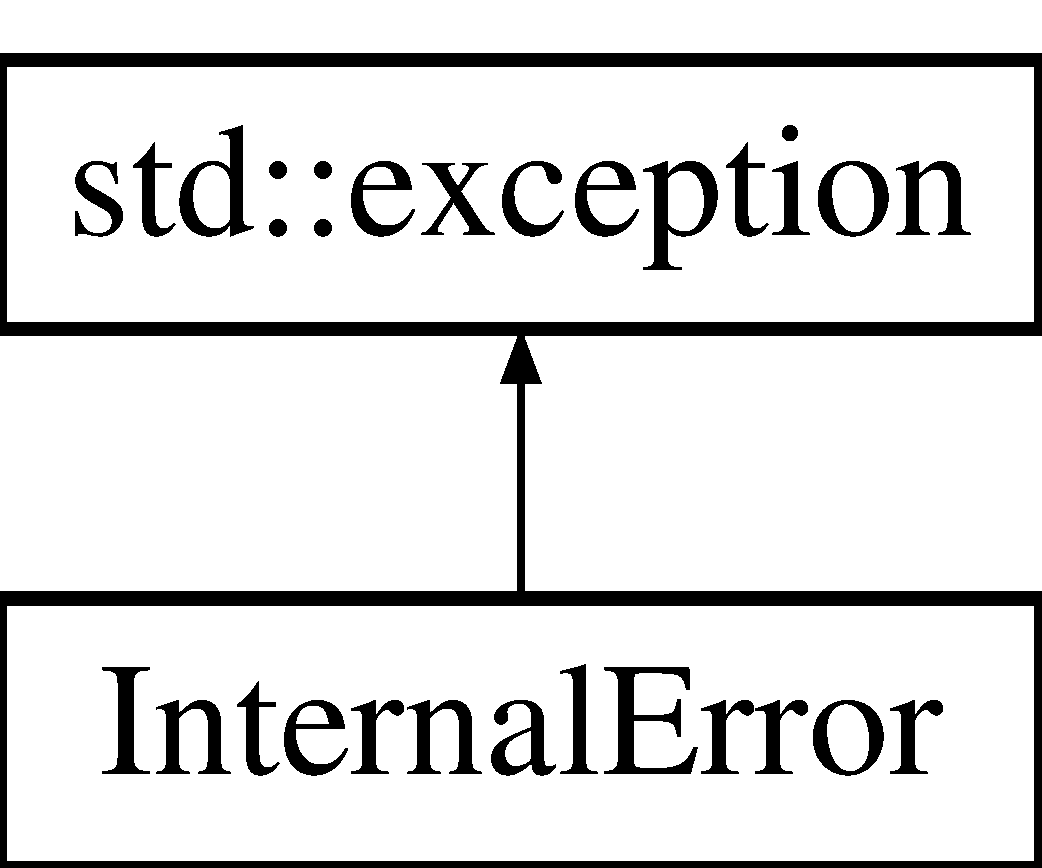
\includegraphics[height=2.000000cm]{classInternalError}
\end{center}
\end{figure}


The documentation for this class was generated from the following file\+:\begin{DoxyCompactItemize}
\item 
include/\hyperlink{common_8h}{common.\+h}\end{DoxyCompactItemize}

\input{classIndexedCorpus_1_1iterator}
\hypertarget{classKeyError}{}\section{Key\+Error Class Reference}
\label{classKeyError}\index{Key\+Error@{Key\+Error}}


{\ttfamily \#include $<$common.\+h$>$}

Inheritance diagram for Key\+Error\+:\begin{figure}[H]
\begin{center}
\leavevmode
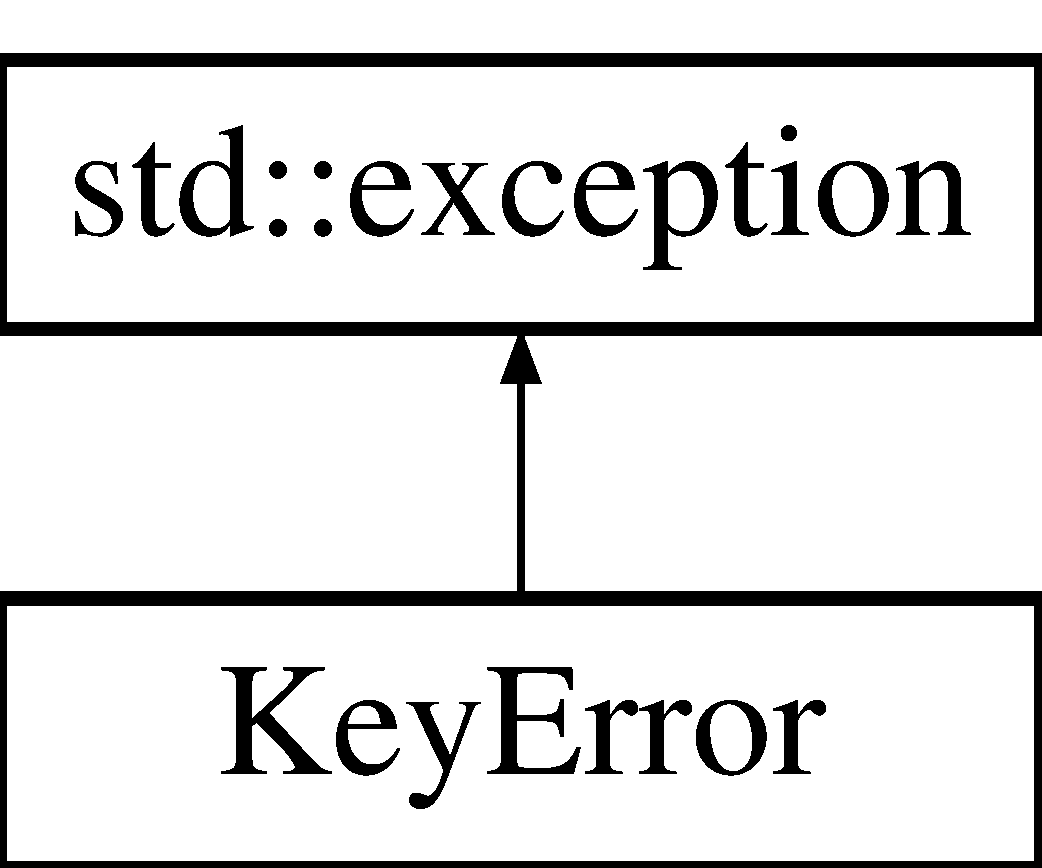
\includegraphics[height=2.000000cm]{classKeyError}
\end{center}
\end{figure}


The documentation for this class was generated from the following file\+:\begin{DoxyCompactItemize}
\item 
include/\hyperlink{common_8h}{common.\+h}\end{DoxyCompactItemize}

\input{structMeasurement}
\hypertarget{classNoSuchPattern}{}\section{No\+Such\+Pattern Class Reference}
\label{classNoSuchPattern}\index{No\+Such\+Pattern@{No\+Such\+Pattern}}


{\ttfamily \#include $<$patternmodel.\+h$>$}

Inheritance diagram for No\+Such\+Pattern\+:\begin{figure}[H]
\begin{center}
\leavevmode
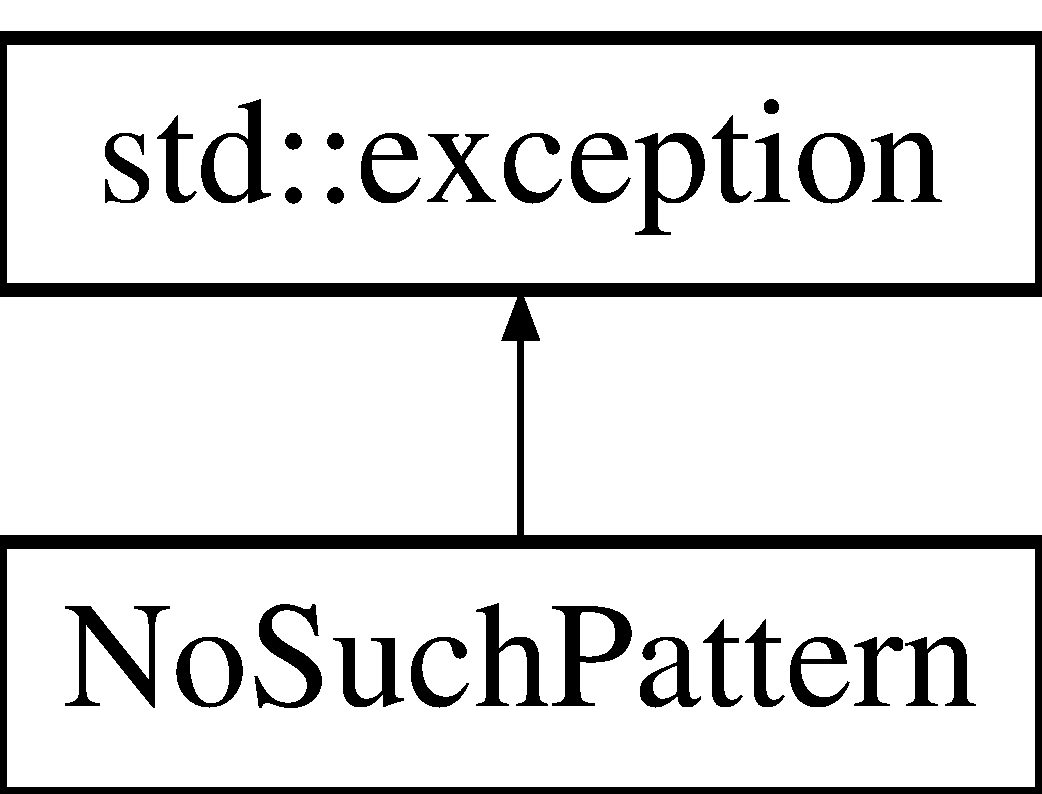
\includegraphics[height=2.000000cm]{classNoSuchPattern}
\end{center}
\end{figure}


The documentation for this class was generated from the following file\+:\begin{DoxyCompactItemize}
\item 
include/\hyperlink{patternmodel_8h}{patternmodel.\+h}\end{DoxyCompactItemize}

\input{classOrderedPatternPointerMap}
\hypertarget{classPattern}{}\section{Pattern Class Reference}
\label{classPattern}\index{Pattern@{Pattern}}


\hyperlink{classPattern}{Pattern} class, represents a pattern (ngram, skipgram or flexgram). Encoded in a memory-\/saving fashion. Allows numerous operations.  




{\ttfamily \#include $<$pattern.\+h$>$}

\subsection*{Public Member Functions}
\begin{DoxyCompactItemize}
\item 
\hyperlink{classPattern_a95f42b0f1717d9e6c2d831e87d27f83c}{Pattern} ()
\item 
\hyperlink{classPattern_a4b345a9704f37489492d769073abe964}{Pattern} (const unsigned char $\ast$dataref, const int \hyperlink{classPattern_a400a18c6a1b6de3eb574b6a0f12c9ca2}{size})
\item 
\hyperlink{classPattern_acba6b63b28a901e6262d1644822c3457}{Pattern} (const \hyperlink{classPattern}{Pattern} \&ref, unsigned int \hyperlink{benchmarks_8cpp_ac7fa37beaab207886901b58632083209}{begin}, unsigned int length)
\item 
\hyperlink{classPattern_ab058696b591b0a157cca3037abcd4afc}{Pattern} (const \hyperlink{classPatternPointer}{Pattern\+Pointer} \&ref, unsigned int \hyperlink{benchmarks_8cpp_ac7fa37beaab207886901b58632083209}{begin}, unsigned int length)
\item 
\hyperlink{classPattern_a9b69825f6e0b1f741be370ac1cbd1b4d}{Pattern} (const \hyperlink{classPattern}{Pattern} \&ref)
\item 
\hyperlink{classPattern_a5731960d41f0f7ffa3e8b03bb519f8b5}{Pattern} (const \hyperlink{classPatternPointer}{Pattern\+Pointer} \&ref)
\item 
\hyperlink{classPattern_a2e658978ef6c0e82ccc85f0b7e59407b}{Pattern} (std\+::istream $\ast$in, bool ignoreeol=false, const unsigned char version=2, const unsigned char $\ast$corpusstart=N\+U\+L\+L, bool debug=false)
\item 
\hyperlink{classPattern_a6e8b9388bbd39934e9f9534b974d7498}{$\sim$\+Pattern} ()
\item 
\hyperlink{classPattern_a80041c82ee57093f673677b22906bbf8}{Pattern} (int \hyperlink{classPattern_a400a18c6a1b6de3eb574b6a0f12c9ca2}{size})
\item 
void \hyperlink{classPattern_ade7dc8f61e70e18004585cd9e50a154c}{write} (std\+::ostream $\ast$\hyperlink{classPattern_ac608089f2fee04e0e8ff6249f14517e4}{out}, const unsigned char $\ast$corpusstart=N\+U\+L\+L) const 
\item 
const size\+\_\+t \hyperlink{classPattern_a13e66bbb8dd77219255ade5aa5f72c7c}{n} () const 
\item 
const size\+\_\+t \hyperlink{classPattern_a57440647189b9e07bdf6ddbcfb0b3f7f}{bytesize} () const 
\item 
const size\+\_\+t \hyperlink{classPattern_a400a18c6a1b6de3eb574b6a0f12c9ca2}{size} () const 
\item 
const unsigned int \hyperlink{classPattern_a0ed5bb99641eb8fd96be7890f2ea5c89}{skipcount} () const 
\item 
const \hyperlink{pattern_8h_a17879f85ec892834fb691c61e71dfe54}{Pattern\+Category} \hyperlink{classPattern_af01c6684c8cec38d3ad57d4303dac5fb}{category} () const 
\item 
const bool \hyperlink{classPattern_a609a2ba1f832678fb69baa201f50b163}{isskipgram} () const 
\item 
const bool \hyperlink{classPattern_a8bef14a88603946827aa1342b47ec001}{isflexgram} () const 
\item 
const bool \hyperlink{classPattern_ad2325ce11035ced772f72dbfd4b57c01}{unknown} () const 
\item 
\hyperlink{classPattern}{Pattern} \hyperlink{classPattern_a96b22b7fdcfde6313ee6c6452c70edbe}{operator\mbox{[}$\,$\mbox{]}} (int index) const 
\item 
const size\+\_\+t \hyperlink{classPattern_a54b434666a79e1567a448eea096dcbb9}{hash} () const 
\item 
std\+::string \hyperlink{classPattern_a810d538d873a823d0b6dbe04d2faf334}{tostring} (const \hyperlink{classClassDecoder}{Class\+Decoder} \&classdecoder) const 
\item 
std\+::string \hyperlink{classPattern_abb031f769621b5a2d5652a29a85b86a2}{decode} (const \hyperlink{classClassDecoder}{Class\+Decoder} \&classdecoder) const 
\item 
bool \hyperlink{classPattern_ac608089f2fee04e0e8ff6249f14517e4}{out} () const 
\item 
std\+::vector$<$ unsigned int $>$ \hyperlink{classPattern_a252702c8acfe5ef9b2aa9783bf4f78ed}{tovector} () const 
\item 
bool \hyperlink{classPattern_a2b5a2c979473b3a62b17128f4c628be2}{operator==} (const \hyperlink{classPattern}{Pattern} \&other) const 
\item 
bool \hyperlink{classPattern_ac02b6479822d7c9ad1beb12dc26eb419}{operator!=} (const \hyperlink{classPattern}{Pattern} \&other) const 
\item 
bool \hyperlink{classPattern_a76f58521a5cfa740d502878bf6924071}{operator==} (const \hyperlink{classPatternPointer}{Pattern\+Pointer} \&other) const 
\item 
bool \hyperlink{classPattern_a272c1d3b0a301b0f11dd5d7a80352ca8}{operator!=} (const \hyperlink{classPatternPointer}{Pattern\+Pointer} \&other) const 
\item 
void \hyperlink{classPattern_ae0ea02ade72a1fe7f92cd48d98754559}{operator=} (const \hyperlink{classPattern}{Pattern} \&other)
\item 
bool \hyperlink{classPattern_aaad79201ca656e519b069cd746722d1b}{operator$<$} (const \hyperlink{classPattern}{Pattern} \&other) const 
\item 
bool \hyperlink{classPattern_a638524274293c8001ec8c605ea5697a5}{operator$>$} (const \hyperlink{classPattern}{Pattern} \&other) const 
\item 
\hyperlink{classPattern}{Pattern} \hyperlink{classPattern_a023243f162cf922306129c14ea7786f7}{operator+} (const \hyperlink{classPattern}{Pattern} \&) const 
\item 
\hyperlink{classPatternPointer}{Pattern\+Pointer} \hyperlink{classPattern_a5f7cc0507ceb4f2e72ac535a32938135}{getpointer} () const 
\item 
int \hyperlink{classPattern_abcd8d461a6c7ebdafe764f959f152c83}{find} (const \hyperlink{classPattern}{Pattern} \&subpattern) const 
\item 
bool \hyperlink{classPattern_aa0de9e5bf5611e8072b0324869e2f782}{contains} (const \hyperlink{classPattern}{Pattern} \&subpattern) const 
\item 
bool \hyperlink{classPattern_a62563035a235a84b77fc4bd97bc82e0e}{instanceof} (const \hyperlink{classPattern}{Pattern} \&skipgram) const 
\item 
int \hyperlink{classPattern_a776b95441fb7c4cdd159c7df7b9097af}{ngrams} (std\+::vector$<$ \hyperlink{classPattern}{Pattern} $>$ \&container, const int \hyperlink{classPattern_a13e66bbb8dd77219255ade5aa5f72c7c}{n}) const 
\item 
int \hyperlink{classPattern_ad2a401cd64493ce88725a14333a3d4e4}{ngrams} (std\+::vector$<$ \hyperlink{classPatternPointer}{Pattern\+Pointer} $>$ \&container, const int \hyperlink{classPattern_a13e66bbb8dd77219255ade5aa5f72c7c}{n}) const 
\item 
int \hyperlink{classPattern_a991dae023a1b507e1f754ad49c31ac88}{subngrams} (std\+::vector$<$ \hyperlink{classPattern}{Pattern} $>$ \&container, int minn=1, int maxn=99) const 
\item 
int \hyperlink{classPattern_af07c1ce51ea00be5df4ea7ab93645ac0}{subngrams} (std\+::vector$<$ \hyperlink{classPatternPointer}{Pattern\+Pointer} $>$ \&container, int minn=1, int maxn=99) const 
\item 
int \hyperlink{classPattern_ad0d0f54adcf6e23070e6761fa1832d3c}{ngrams} (std\+::vector$<$ std\+::pair$<$ \hyperlink{classPattern}{Pattern}, int $>$$>$ \&container, const int \hyperlink{classPattern_a13e66bbb8dd77219255ade5aa5f72c7c}{n}) const 
\item 
int \hyperlink{classPattern_a85c317920a643e765fc51f6f14e2a474}{ngrams} (std\+::vector$<$ std\+::pair$<$ \hyperlink{classPatternPointer}{Pattern\+Pointer}, int $>$$>$ \&container, const int \hyperlink{classPattern_a13e66bbb8dd77219255ade5aa5f72c7c}{n}) const 
\item 
int \hyperlink{classPattern_af74f62b5d7cb9b831025340ff7b62ea4}{subngrams} (std\+::vector$<$ std\+::pair$<$ \hyperlink{classPattern}{Pattern}, int $>$$>$ \&container, int minn=1, int maxn=9) const 
\item 
int \hyperlink{classPattern_af64bc5357eb5c30128e0a4f13243cd2a}{subngrams} (std\+::vector$<$ std\+::pair$<$ \hyperlink{classPatternPointer}{Pattern\+Pointer}, int $>$$>$ \&container, int minn=1, int maxn=9) const 
\item 
int \hyperlink{classPattern_a615d0bd0b135804c993ce0fb027c5491}{parts} (std\+::vector$<$ \hyperlink{classPattern}{Pattern} $>$ \&container) const 
\item 
int \hyperlink{classPattern_a77fcd5463f55ff890139d7c6dee1695b}{parts} (std\+::vector$<$ \hyperlink{classPatternPointer}{Pattern\+Pointer} $>$ \&container) const 
\item 
int \hyperlink{classPattern_acde3a00e476df661b46cc28318e32077}{parts} (std\+::vector$<$ std\+::pair$<$ int, int $>$ $>$ \&container) const 
\item 
int \hyperlink{classPattern_ad4dd286b352c7e5e66dd73233b0d6b29}{gaps} (std\+::vector$<$ std\+::pair$<$ int, int $>$ $>$ \&container) const 
\item 
\hyperlink{classPattern}{Pattern} \hyperlink{classPattern_a5c6f31402871dbac582b22c0c585309c}{extractskipcontent} (const \hyperlink{classPattern}{Pattern} \&instance) const 
\item 
\hyperlink{classPattern}{Pattern} \hyperlink{classPattern_afab002bc06207214e84ff324becfe224}{replace} (int \hyperlink{benchmarks_8cpp_ac7fa37beaab207886901b58632083209}{begin}, int length, const \hyperlink{classPattern}{Pattern} \&replacement) const 
\item 
\hyperlink{classPattern}{Pattern} \hyperlink{classPattern_a7eee8becce24d9e3ff8c72d65af0856d}{addskip} (const std\+::pair$<$ int, int $>$ \&gap) const 
\item 
\hyperlink{classPattern}{Pattern} \hyperlink{classPattern_acb62137cc96984adba34ca4a1b857dc9}{addskips} (const std\+::vector$<$ std\+::pair$<$ int, int $>$ $>$ \&\hyperlink{classPattern_ad4dd286b352c7e5e66dd73233b0d6b29}{gaps}) const 
\item 
\hyperlink{classPattern}{Pattern} \hyperlink{classPattern_acb0a3e2954c8f74cfa853748e4423fa4}{addflexgaps} (const std\+::vector$<$ std\+::pair$<$ int, int $>$ $>$ \&\hyperlink{classPattern_ad4dd286b352c7e5e66dd73233b0d6b29}{gaps}) const 
\item 
\hyperlink{classPattern}{Pattern} \hyperlink{classPattern_a15e028c7c47223bec756f9a50c9d3fd0}{reverse} () const 
\item 
\hyperlink{classPattern}{Pattern} \hyperlink{classPattern_a542295a795ff5a906044dd9b6b550f0e}{toflexgram} () const 
\item 
bool \hyperlink{classPattern_a971a055b02cf2c7d6f0c6a5a0e4401f0}{isgap} (int i) const 
\item 
\hyperlink{classPattern}{Pattern} \hyperlink{classPattern_ae9b514ce75a9e8a32407684167b8ce99}{addcontext} (const \hyperlink{classPattern}{Pattern} \&leftcontext, const \hyperlink{classPattern}{Pattern} \&rightcontext) const 
\item 
void \hyperlink{classPattern_a1388ffcf485ba7a32417e6a442338f44}{mask} (std\+::vector$<$ bool $>$ \&container) const 
\item 
void \hyperlink{classPattern_afc9539da36985d942552620ea2f26525}{set} (const unsigned char $\ast$dataref, const int \hyperlink{classPattern_a400a18c6a1b6de3eb574b6a0f12c9ca2}{size})
\end{DoxyCompactItemize}
\subsection*{Public Attributes}
\begin{DoxyCompactItemize}
\item 
unsigned char $\ast$ \hyperlink{classPattern_a2e20f4d132daff981db27bb13d3ff2b5}{data}
\end{DoxyCompactItemize}
\subsection*{Static Public Attributes}
\begin{DoxyCompactItemize}
\item 
static const int \hyperlink{classPattern_ab48e128327c90c9c250a6b0d7e8362a3}{patterntype} = \hyperlink{pattern_8h_a351dc5aa88481a949638aeb6cc5e6754ac2ab7901214563c5f2300c42358129f6}{P\+A\+T\+T\+E\+R\+N}
\end{DoxyCompactItemize}


\subsection{Detailed Description}
\hyperlink{classPattern}{Pattern} class, represents a pattern (ngram, skipgram or flexgram). Encoded in a memory-\/saving fashion. Allows numerous operations. 

\subsection{Constructor \& Destructor Documentation}
\hypertarget{classPattern_a95f42b0f1717d9e6c2d831e87d27f83c}{}\index{Pattern@{Pattern}!Pattern@{Pattern}}
\index{Pattern@{Pattern}!Pattern@{Pattern}}
\subsubsection[{Pattern()}]{\setlength{\rightskip}{0pt plus 5cm}Pattern\+::\+Pattern (
\begin{DoxyParamCaption}
{}
\end{DoxyParamCaption}
)\hspace{0.3cm}{\ttfamily [inline]}}\label{classPattern_a95f42b0f1717d9e6c2d831e87d27f83c}
Default/empty \hyperlink{classPattern}{Pattern} constructor. Creates an empty pattern. Still consumes one byte (the end-\/marker) \hypertarget{classPattern_a4b345a9704f37489492d769073abe964}{}\index{Pattern@{Pattern}!Pattern@{Pattern}}
\index{Pattern@{Pattern}!Pattern@{Pattern}}
\subsubsection[{Pattern(const unsigned char $\ast$dataref, const int size)}]{\setlength{\rightskip}{0pt plus 5cm}Pattern\+::\+Pattern (
\begin{DoxyParamCaption}
\item[{const unsigned char $\ast$}]{dataref, }
\item[{const int}]{size}
\end{DoxyParamCaption}
)}\label{classPattern_a4b345a9704f37489492d769073abe964}
Low-\/level pattern constructor from character array. The size is in bytes and never includes the end-\/marker. 
\begin{DoxyParams}{Parameters}
{\em dataref} & Reference data, must be properly class-\/encoded \\
\hline
{\em size} & The size (without \textbackslash{}0 end marker!) to copy from dataref \\
\hline
\end{DoxyParams}
\hypertarget{classPattern_acba6b63b28a901e6262d1644822c3457}{}\index{Pattern@{Pattern}!Pattern@{Pattern}}
\index{Pattern@{Pattern}!Pattern@{Pattern}}
\subsubsection[{Pattern(const Pattern \&ref, unsigned int begin, unsigned int length)}]{\setlength{\rightskip}{0pt plus 5cm}Pattern\+::\+Pattern (
\begin{DoxyParamCaption}
\item[{const {\bf Pattern} \&}]{ref, }
\item[{unsigned int}]{begin, }
\item[{unsigned int}]{length}
\end{DoxyParamCaption}
)}\label{classPattern_acba6b63b28a901e6262d1644822c3457}
Slice constructor for \hyperlink{classPattern}{Pattern} 
\begin{DoxyParams}{Parameters}
{\em ref} & Reference pattern \\
\hline
{\em begin} & Index of the first token to copy (0-\/indexed) \\
\hline
{\em length} & Number of tokens to copy \\
\hline
\end{DoxyParams}
\hypertarget{classPattern_ab058696b591b0a157cca3037abcd4afc}{}\index{Pattern@{Pattern}!Pattern@{Pattern}}
\index{Pattern@{Pattern}!Pattern@{Pattern}}
\subsubsection[{Pattern(const Pattern\+Pointer \&ref, unsigned int begin, unsigned int length)}]{\setlength{\rightskip}{0pt plus 5cm}Pattern\+::\+Pattern (
\begin{DoxyParamCaption}
\item[{const {\bf Pattern\+Pointer} \&}]{ref, }
\item[{unsigned int}]{begin, }
\item[{unsigned int}]{length}
\end{DoxyParamCaption}
)}\label{classPattern_ab058696b591b0a157cca3037abcd4afc}
\hypertarget{classPattern_a9b69825f6e0b1f741be370ac1cbd1b4d}{}\index{Pattern@{Pattern}!Pattern@{Pattern}}
\index{Pattern@{Pattern}!Pattern@{Pattern}}
\subsubsection[{Pattern(const Pattern \&ref)}]{\setlength{\rightskip}{0pt plus 5cm}Pattern\+::\+Pattern (
\begin{DoxyParamCaption}
\item[{const {\bf Pattern} \&}]{ref}
\end{DoxyParamCaption}
)}\label{classPattern_a9b69825f6e0b1f741be370ac1cbd1b4d}
Copy constructor for \hyperlink{classPattern}{Pattern} 
\begin{DoxyParams}{Parameters}
{\em ref} & Reference pattern \\
\hline
\end{DoxyParams}
\hypertarget{classPattern_a5731960d41f0f7ffa3e8b03bb519f8b5}{}\index{Pattern@{Pattern}!Pattern@{Pattern}}
\index{Pattern@{Pattern}!Pattern@{Pattern}}
\subsubsection[{Pattern(const Pattern\+Pointer \&ref)}]{\setlength{\rightskip}{0pt plus 5cm}Pattern\+::\+Pattern (
\begin{DoxyParamCaption}
\item[{const {\bf Pattern\+Pointer} \&}]{ref}
\end{DoxyParamCaption}
)}\label{classPattern_a5731960d41f0f7ffa3e8b03bb519f8b5}
\hypertarget{classPattern_a2e658978ef6c0e82ccc85f0b7e59407b}{}\index{Pattern@{Pattern}!Pattern@{Pattern}}
\index{Pattern@{Pattern}!Pattern@{Pattern}}
\subsubsection[{Pattern(std\+::istream $\ast$in, bool ignoreeol=false, const unsigned char version=2, const unsigned char $\ast$corpusstart=\+N\+U\+L\+L, bool debug=false)}]{\setlength{\rightskip}{0pt plus 5cm}Pattern\+::\+Pattern (
\begin{DoxyParamCaption}
\item[{std\+::istream $\ast$}]{in, }
\item[{bool}]{ignoreeol = {\ttfamily false}, }
\item[{const unsigned char}]{version = {\ttfamily 2}, }
\item[{const unsigned char $\ast$}]{corpusstart = {\ttfamily NULL}, }
\item[{bool}]{debug = {\ttfamily false}}
\end{DoxyParamCaption}
)}\label{classPattern_a2e658978ef6c0e82ccc85f0b7e59407b}
Read \hyperlink{classPattern}{Pattern} from input stream (in binary form) 
\begin{DoxyParams}{Parameters}
{\em in} & The input stream \\
\hline
{\em ignoreeol} & Ignore end of line markers and read on until the end of the file, storing corpus data in one pattern \\
\hline
{\em version} & Version of file format (default\+: 2) \\
\hline
{\em corpusoffset} & not used \\
\hline
\end{DoxyParams}
\hypertarget{classPattern_a6e8b9388bbd39934e9f9534b974d7498}{}\index{Pattern@{Pattern}!````~Pattern@{$\sim$\+Pattern}}
\index{````~Pattern@{$\sim$\+Pattern}!Pattern@{Pattern}}
\subsubsection[{$\sim$\+Pattern()}]{\setlength{\rightskip}{0pt plus 5cm}Pattern\+::$\sim$\+Pattern (
\begin{DoxyParamCaption}
{}
\end{DoxyParamCaption}
)}\label{classPattern_a6e8b9388bbd39934e9f9534b974d7498}
\hypertarget{classPattern_a80041c82ee57093f673677b22906bbf8}{}\index{Pattern@{Pattern}!Pattern@{Pattern}}
\index{Pattern@{Pattern}!Pattern@{Pattern}}
\subsubsection[{Pattern(int size)}]{\setlength{\rightskip}{0pt plus 5cm}Pattern\+::\+Pattern (
\begin{DoxyParamCaption}
\item[{int}]{size}
\end{DoxyParamCaption}
)\hspace{0.3cm}{\ttfamily [inline]}}\label{classPattern_a80041c82ee57093f673677b22906bbf8}
\hyperlink{classPattern}{Pattern} constructor consisting of only a fixed-\/size gap 
\begin{DoxyParams}{Parameters}
{\em size} & The size of the gap \\
\hline
\end{DoxyParams}


\subsection{Member Function Documentation}
\hypertarget{classPattern_ae9b514ce75a9e8a32407684167b8ce99}{}\index{Pattern@{Pattern}!addcontext@{addcontext}}
\index{addcontext@{addcontext}!Pattern@{Pattern}}
\subsubsection[{addcontext(const Pattern \&leftcontext, const Pattern \&rightcontext) const }]{\setlength{\rightskip}{0pt plus 5cm}{\bf Pattern} Pattern\+::addcontext (
\begin{DoxyParamCaption}
\item[{const {\bf Pattern} \&}]{leftcontext, }
\item[{const {\bf Pattern} \&}]{rightcontext}
\end{DoxyParamCaption}
) const}\label{classPattern_ae9b514ce75a9e8a32407684167b8ce99}
\hypertarget{classPattern_acb0a3e2954c8f74cfa853748e4423fa4}{}\index{Pattern@{Pattern}!addflexgaps@{addflexgaps}}
\index{addflexgaps@{addflexgaps}!Pattern@{Pattern}}
\subsubsection[{addflexgaps(const std\+::vector$<$ std\+::pair$<$ int, int $>$ $>$ \&gaps) const }]{\setlength{\rightskip}{0pt plus 5cm}{\bf Pattern} Pattern\+::addflexgaps (
\begin{DoxyParamCaption}
\item[{const std\+::vector$<$ std\+::pair$<$ int, int $>$ $>$ \&}]{gaps}
\end{DoxyParamCaption}
) const}\label{classPattern_acb0a3e2954c8f74cfa853748e4423fa4}
Replaces multiple series of tokens with skips/gaps of undefined variable size. Effectively turns a pattern into a flexgram. 
\begin{DoxyParams}{Parameters}
{\em gaps} & The positions and sizes of the gaps\+: a vector of pairs, each pair consisting of a begin index (0-\/indexed) and a length, indicating where to place the gap \\
\hline
\end{DoxyParams}
\begin{DoxyReturn}{Returns}
A flexgram 
\end{DoxyReturn}
\hypertarget{classPattern_a7eee8becce24d9e3ff8c72d65af0856d}{}\index{Pattern@{Pattern}!addskip@{addskip}}
\index{addskip@{addskip}!Pattern@{Pattern}}
\subsubsection[{addskip(const std\+::pair$<$ int, int $>$ \&gap) const }]{\setlength{\rightskip}{0pt plus 5cm}{\bf Pattern} Pattern\+::addskip (
\begin{DoxyParamCaption}
\item[{const std\+::pair$<$ int, int $>$ \&}]{gap}
\end{DoxyParamCaption}
) const}\label{classPattern_a7eee8becce24d9e3ff8c72d65af0856d}
Replaces a series of tokens with a skip/gap of a particular size. Effectively turns a pattern into a skipgram. 
\begin{DoxyParams}{Parameters}
{\em gap} & The position and size of the skip/gap\+: a pair consisting of a begin index (0-\/indexed) and a length, i.\+e. the size of the skip \\
\hline
\end{DoxyParams}
\hypertarget{classPattern_acb62137cc96984adba34ca4a1b857dc9}{}\index{Pattern@{Pattern}!addskips@{addskips}}
\index{addskips@{addskips}!Pattern@{Pattern}}
\subsubsection[{addskips(const std\+::vector$<$ std\+::pair$<$ int, int $>$ $>$ \&gaps) const }]{\setlength{\rightskip}{0pt plus 5cm}{\bf Pattern} Pattern\+::addskips (
\begin{DoxyParamCaption}
\item[{const std\+::vector$<$ std\+::pair$<$ int, int $>$ $>$ \&}]{gaps}
\end{DoxyParamCaption}
) const}\label{classPattern_acb62137cc96984adba34ca4a1b857dc9}
Replaces multiple series of tokens with skips/gaps of particular sizes. Effectively turns a pattern into a skipgram. 
\begin{DoxyParams}{Parameters}
{\em gaps} & The positions and sizes of the gaps\+: a vector of pairs, each pair consisting of a begin index (0-\/indexed) and a length, indicating where to place the gap \\
\hline
\end{DoxyParams}
\begin{DoxyReturn}{Returns}
A skipgram 
\end{DoxyReturn}
\hypertarget{classPattern_a57440647189b9e07bdf6ddbcfb0b3f7f}{}\index{Pattern@{Pattern}!bytesize@{bytesize}}
\index{bytesize@{bytesize}!Pattern@{Pattern}}
\subsubsection[{bytesize() const }]{\setlength{\rightskip}{0pt plus 5cm}const size\+\_\+t Pattern\+::bytesize (
\begin{DoxyParamCaption}
{}
\end{DoxyParamCaption}
) const}\label{classPattern_a57440647189b9e07bdf6ddbcfb0b3f7f}
return the size of the pattern (in bytes), this does not include the final \textbackslash{}0 end-\/marker. \hypertarget{classPattern_af01c6684c8cec38d3ad57d4303dac5fb}{}\index{Pattern@{Pattern}!category@{category}}
\index{category@{category}!Pattern@{Pattern}}
\subsubsection[{category() const }]{\setlength{\rightskip}{0pt plus 5cm}const {\bf Pattern\+Category} Pattern\+::category (
\begin{DoxyParamCaption}
{}
\end{DoxyParamCaption}
) const}\label{classPattern_af01c6684c8cec38d3ad57d4303dac5fb}
Returns the category of this pattern (value from enum Pattern\+Category) \hypertarget{classPattern_aa0de9e5bf5611e8072b0324869e2f782}{}\index{Pattern@{Pattern}!contains@{contains}}
\index{contains@{contains}!Pattern@{Pattern}}
\subsubsection[{contains(const Pattern \&subpattern) const }]{\setlength{\rightskip}{0pt plus 5cm}bool Pattern\+::contains (
\begin{DoxyParamCaption}
\item[{const {\bf Pattern} \&}]{subpattern}
\end{DoxyParamCaption}
) const}\label{classPattern_aa0de9e5bf5611e8072b0324869e2f782}
Test whether the pattern contains the specified subpattern. \hypertarget{classPattern_abb031f769621b5a2d5652a29a85b86a2}{}\index{Pattern@{Pattern}!decode@{decode}}
\index{decode@{decode}!Pattern@{Pattern}}
\subsubsection[{decode(const Class\+Decoder \&classdecoder) const }]{\setlength{\rightskip}{0pt plus 5cm}std\+::string Pattern\+::decode (
\begin{DoxyParamCaption}
\item[{const {\bf Class\+Decoder} \&}]{classdecoder}
\end{DoxyParamCaption}
) const\hspace{0.3cm}{\ttfamily [inline]}}\label{classPattern_abb031f769621b5a2d5652a29a85b86a2}
alias for \hyperlink{classPattern_a810d538d873a823d0b6dbe04d2faf334}{tostring()} \hypertarget{classPattern_a5c6f31402871dbac582b22c0c585309c}{}\index{Pattern@{Pattern}!extractskipcontent@{extractskipcontent}}
\index{extractskipcontent@{extractskipcontent}!Pattern@{Pattern}}
\subsubsection[{extractskipcontent(const Pattern \&instance) const }]{\setlength{\rightskip}{0pt plus 5cm}{\bf Pattern} Pattern\+::extractskipcontent (
\begin{DoxyParamCaption}
\item[{const {\bf Pattern} \&}]{instance}
\end{DoxyParamCaption}
) const}\label{classPattern_a5c6f31402871dbac582b22c0c585309c}
Given a skipgram and an ngram instantation of it (i.\+e, both of the same length), extract a pattern from the instance that would fill the gaps. Raise an exception if the instance can not be matched with the skipgram \hypertarget{classPattern_abcd8d461a6c7ebdafe764f959f152c83}{}\index{Pattern@{Pattern}!find@{find}}
\index{find@{find}!Pattern@{Pattern}}
\subsubsection[{find(const Pattern \&subpattern) const }]{\setlength{\rightskip}{0pt plus 5cm}int Pattern\+::find (
\begin{DoxyParamCaption}
\item[{const {\bf Pattern} \&}]{subpattern}
\end{DoxyParamCaption}
) const}\label{classPattern_abcd8d461a6c7ebdafe764f959f152c83}
Finds the specified subpattern in the this pattern. Returns the index at which it is found, or -\/1 if it is not found at all. \hypertarget{classPattern_ad4dd286b352c7e5e66dd73233b0d6b29}{}\index{Pattern@{Pattern}!gaps@{gaps}}
\index{gaps@{gaps}!Pattern@{Pattern}}
\subsubsection[{gaps(std\+::vector$<$ std\+::pair$<$ int, int $>$ $>$ \&container) const }]{\setlength{\rightskip}{0pt plus 5cm}int Pattern\+::gaps (
\begin{DoxyParamCaption}
\item[{std\+::vector$<$ std\+::pair$<$ int, int $>$ $>$ \&}]{container}
\end{DoxyParamCaption}
) const}\label{classPattern_ad4dd286b352c7e5e66dd73233b0d6b29}
Finds all the gaps of a skipgram or flexgram., parts are the portions that are not skips and adds them to container as begin,length pairs... Thus \textquotesingle{}to be \{$\ast$\} not \{$\ast$\} be\textquotesingle{} has three parts. The gap-\/length of a flexgram will always be its minimum length one. \hypertarget{classPattern_a5f7cc0507ceb4f2e72ac535a32938135}{}\index{Pattern@{Pattern}!getpointer@{getpointer}}
\index{getpointer@{getpointer}!Pattern@{Pattern}}
\subsubsection[{getpointer() const }]{\setlength{\rightskip}{0pt plus 5cm}{\bf Pattern\+Pointer} Pattern\+::getpointer (
\begin{DoxyParamCaption}
{}
\end{DoxyParamCaption}
) const}\label{classPattern_a5f7cc0507ceb4f2e72ac535a32938135}
\hypertarget{classPattern_a54b434666a79e1567a448eea096dcbb9}{}\index{Pattern@{Pattern}!hash@{hash}}
\index{hash@{hash}!Pattern@{Pattern}}
\subsubsection[{hash() const }]{\setlength{\rightskip}{0pt plus 5cm}const size\+\_\+t Pattern\+::hash (
\begin{DoxyParamCaption}
{}
\end{DoxyParamCaption}
) const}\label{classPattern_a54b434666a79e1567a448eea096dcbb9}
Compute a hash value for this pattern \hypertarget{classPattern_a62563035a235a84b77fc4bd97bc82e0e}{}\index{Pattern@{Pattern}!instanceof@{instanceof}}
\index{instanceof@{instanceof}!Pattern@{Pattern}}
\subsubsection[{instanceof(const Pattern \&skipgram) const }]{\setlength{\rightskip}{0pt plus 5cm}bool Pattern\+::instanceof (
\begin{DoxyParamCaption}
\item[{const {\bf Pattern} \&}]{skipgram}
\end{DoxyParamCaption}
) const}\label{classPattern_a62563035a235a84b77fc4bd97bc82e0e}
Tests whether the pattern is an instantiation of the specified skipgram \hypertarget{classPattern_a8bef14a88603946827aa1342b47ec001}{}\index{Pattern@{Pattern}!isflexgram@{isflexgram}}
\index{isflexgram@{isflexgram}!Pattern@{Pattern}}
\subsubsection[{isflexgram() const }]{\setlength{\rightskip}{0pt plus 5cm}const bool Pattern\+::isflexgram (
\begin{DoxyParamCaption}
{}
\end{DoxyParamCaption}
) const\hspace{0.3cm}{\ttfamily [inline]}}\label{classPattern_a8bef14a88603946827aa1342b47ec001}
\hypertarget{classPattern_a971a055b02cf2c7d6f0c6a5a0e4401f0}{}\index{Pattern@{Pattern}!isgap@{isgap}}
\index{isgap@{isgap}!Pattern@{Pattern}}
\subsubsection[{isgap(int i) const }]{\setlength{\rightskip}{0pt plus 5cm}bool Pattern\+::isgap (
\begin{DoxyParamCaption}
\item[{int}]{i}
\end{DoxyParamCaption}
) const}\label{classPattern_a971a055b02cf2c7d6f0c6a5a0e4401f0}
Is the word at the specified index (0 indexed) a gap? \hypertarget{classPattern_a609a2ba1f832678fb69baa201f50b163}{}\index{Pattern@{Pattern}!isskipgram@{isskipgram}}
\index{isskipgram@{isskipgram}!Pattern@{Pattern}}
\subsubsection[{isskipgram() const }]{\setlength{\rightskip}{0pt plus 5cm}const bool Pattern\+::isskipgram (
\begin{DoxyParamCaption}
{}
\end{DoxyParamCaption}
) const\hspace{0.3cm}{\ttfamily [inline]}}\label{classPattern_a609a2ba1f832678fb69baa201f50b163}
\hypertarget{classPattern_a1388ffcf485ba7a32417e6a442338f44}{}\index{Pattern@{Pattern}!mask@{mask}}
\index{mask@{mask}!Pattern@{Pattern}}
\subsubsection[{mask(std\+::vector$<$ bool $>$ \&container) const }]{\setlength{\rightskip}{0pt plus 5cm}void Pattern\+::mask (
\begin{DoxyParamCaption}
\item[{std\+::vector$<$ bool $>$ \&}]{container}
\end{DoxyParamCaption}
) const}\label{classPattern_a1388ffcf485ba7a32417e6a442338f44}
\hypertarget{classPattern_a13e66bbb8dd77219255ade5aa5f72c7c}{}\index{Pattern@{Pattern}!n@{n}}
\index{n@{n}!Pattern@{Pattern}}
\subsubsection[{n() const }]{\setlength{\rightskip}{0pt plus 5cm}const size\+\_\+t Pattern\+::n (
\begin{DoxyParamCaption}
{}
\end{DoxyParamCaption}
) const}\label{classPattern_a13e66bbb8dd77219255ade5aa5f72c7c}
return the size of the pattern in tokens (will count flex gaps gaps as size 1) \hypertarget{classPattern_a776b95441fb7c4cdd159c7df7b9097af}{}\index{Pattern@{Pattern}!ngrams@{ngrams}}
\index{ngrams@{ngrams}!Pattern@{Pattern}}
\subsubsection[{ngrams(std\+::vector$<$ Pattern $>$ \&container, const int n) const }]{\setlength{\rightskip}{0pt plus 5cm}int Pattern\+::ngrams (
\begin{DoxyParamCaption}
\item[{std\+::vector$<$ {\bf Pattern} $>$ \&}]{container, }
\item[{const int}]{n}
\end{DoxyParamCaption}
) const}\label{classPattern_a776b95441fb7c4cdd159c7df7b9097af}
Adds all patterns (not just ngrams) of size n that are contained within the pattern to container. Does not extract skipgrams that are not directly present in the pattern. \hypertarget{classPattern_ad2a401cd64493ce88725a14333a3d4e4}{}\index{Pattern@{Pattern}!ngrams@{ngrams}}
\index{ngrams@{ngrams}!Pattern@{Pattern}}
\subsubsection[{ngrams(std\+::vector$<$ Pattern\+Pointer $>$ \&container, const int n) const }]{\setlength{\rightskip}{0pt plus 5cm}int Pattern\+::ngrams (
\begin{DoxyParamCaption}
\item[{std\+::vector$<$ {\bf Pattern\+Pointer} $>$ \&}]{container, }
\item[{const int}]{n}
\end{DoxyParamCaption}
) const}\label{classPattern_ad2a401cd64493ce88725a14333a3d4e4}
\hypertarget{classPattern_ad0d0f54adcf6e23070e6761fa1832d3c}{}\index{Pattern@{Pattern}!ngrams@{ngrams}}
\index{ngrams@{ngrams}!Pattern@{Pattern}}
\subsubsection[{ngrams(std\+::vector$<$ std\+::pair$<$ Pattern, int $>$$>$ \&container, const int n) const }]{\setlength{\rightskip}{0pt plus 5cm}int Pattern\+::ngrams (
\begin{DoxyParamCaption}
\item[{std\+::vector$<$ std\+::pair$<$ {\bf Pattern}, int $>$$>$ \&}]{container, }
\item[{const int}]{n}
\end{DoxyParamCaption}
) const}\label{classPattern_ad0d0f54adcf6e23070e6761fa1832d3c}
Adds all pairs of all patterns (not just ngrams) of size n that are contained within the pattern, with the token offset at which they were found, to container. Does not extract skipgrams that are not directly present in the pattern. \hypertarget{classPattern_a85c317920a643e765fc51f6f14e2a474}{}\index{Pattern@{Pattern}!ngrams@{ngrams}}
\index{ngrams@{ngrams}!Pattern@{Pattern}}
\subsubsection[{ngrams(std\+::vector$<$ std\+::pair$<$ Pattern\+Pointer, int $>$$>$ \&container, const int n) const }]{\setlength{\rightskip}{0pt plus 5cm}int Pattern\+::ngrams (
\begin{DoxyParamCaption}
\item[{std\+::vector$<$ std\+::pair$<$ {\bf Pattern\+Pointer}, int $>$$>$ \&}]{container, }
\item[{const int}]{n}
\end{DoxyParamCaption}
) const}\label{classPattern_a85c317920a643e765fc51f6f14e2a474}
\hypertarget{classPattern_ac02b6479822d7c9ad1beb12dc26eb419}{}\index{Pattern@{Pattern}!operator"!=@{operator"!=}}
\index{operator"!=@{operator"!=}!Pattern@{Pattern}}
\subsubsection[{operator"!=(const Pattern \&other) const }]{\setlength{\rightskip}{0pt plus 5cm}bool Pattern\+::operator!= (
\begin{DoxyParamCaption}
\item[{const {\bf Pattern} \&}]{other}
\end{DoxyParamCaption}
) const}\label{classPattern_ac02b6479822d7c9ad1beb12dc26eb419}
\hypertarget{classPattern_a272c1d3b0a301b0f11dd5d7a80352ca8}{}\index{Pattern@{Pattern}!operator"!=@{operator"!=}}
\index{operator"!=@{operator"!=}!Pattern@{Pattern}}
\subsubsection[{operator"!=(const Pattern\+Pointer \&other) const }]{\setlength{\rightskip}{0pt plus 5cm}bool Pattern\+::operator!= (
\begin{DoxyParamCaption}
\item[{const {\bf Pattern\+Pointer} \&}]{other}
\end{DoxyParamCaption}
) const}\label{classPattern_a272c1d3b0a301b0f11dd5d7a80352ca8}
\hypertarget{classPattern_a023243f162cf922306129c14ea7786f7}{}\index{Pattern@{Pattern}!operator+@{operator+}}
\index{operator+@{operator+}!Pattern@{Pattern}}
\subsubsection[{operator+(const Pattern \&) const }]{\setlength{\rightskip}{0pt plus 5cm}{\bf Pattern} Pattern\+::operator+ (
\begin{DoxyParamCaption}
\item[{const {\bf Pattern} \&}]{other}
\end{DoxyParamCaption}
) const}\label{classPattern_a023243f162cf922306129c14ea7786f7}
\hypertarget{classPattern_aaad79201ca656e519b069cd746722d1b}{}\index{Pattern@{Pattern}!operator$<$@{operator$<$}}
\index{operator$<$@{operator$<$}!Pattern@{Pattern}}
\subsubsection[{operator$<$(const Pattern \&other) const }]{\setlength{\rightskip}{0pt plus 5cm}bool Pattern\+::operator$<$ (
\begin{DoxyParamCaption}
\item[{const {\bf Pattern} \&}]{other}
\end{DoxyParamCaption}
) const}\label{classPattern_aaad79201ca656e519b069cd746722d1b}
Patterns can be sorted, note however that the sorting is based on the frequencies of the tokens and is not alphanumerical! \hypertarget{classPattern_ae0ea02ade72a1fe7f92cd48d98754559}{}\index{Pattern@{Pattern}!operator=@{operator=}}
\index{operator=@{operator=}!Pattern@{Pattern}}
\subsubsection[{operator=(const Pattern \&other)}]{\setlength{\rightskip}{0pt plus 5cm}void Pattern\+::operator= (
\begin{DoxyParamCaption}
\item[{const {\bf Pattern} \&}]{other}
\end{DoxyParamCaption}
)}\label{classPattern_ae0ea02ade72a1fe7f92cd48d98754559}
Assignment operator \hypertarget{classPattern_a2b5a2c979473b3a62b17128f4c628be2}{}\index{Pattern@{Pattern}!operator==@{operator==}}
\index{operator==@{operator==}!Pattern@{Pattern}}
\subsubsection[{operator==(const Pattern \&other) const }]{\setlength{\rightskip}{0pt plus 5cm}bool Pattern\+::operator== (
\begin{DoxyParamCaption}
\item[{const {\bf Pattern} \&}]{other}
\end{DoxyParamCaption}
) const}\label{classPattern_a2b5a2c979473b3a62b17128f4c628be2}
\hypertarget{classPattern_a76f58521a5cfa740d502878bf6924071}{}\index{Pattern@{Pattern}!operator==@{operator==}}
\index{operator==@{operator==}!Pattern@{Pattern}}
\subsubsection[{operator==(const Pattern\+Pointer \&other) const }]{\setlength{\rightskip}{0pt plus 5cm}bool Pattern\+::operator== (
\begin{DoxyParamCaption}
\item[{const {\bf Pattern\+Pointer} \&}]{other}
\end{DoxyParamCaption}
) const}\label{classPattern_a76f58521a5cfa740d502878bf6924071}
\hypertarget{classPattern_a638524274293c8001ec8c605ea5697a5}{}\index{Pattern@{Pattern}!operator$>$@{operator$>$}}
\index{operator$>$@{operator$>$}!Pattern@{Pattern}}
\subsubsection[{operator$>$(const Pattern \&other) const }]{\setlength{\rightskip}{0pt plus 5cm}bool Pattern\+::operator$>$ (
\begin{DoxyParamCaption}
\item[{const {\bf Pattern} \&}]{other}
\end{DoxyParamCaption}
) const}\label{classPattern_a638524274293c8001ec8c605ea5697a5}
\hypertarget{classPattern_a96b22b7fdcfde6313ee6c6452c70edbe}{}\index{Pattern@{Pattern}!operator\mbox{[}$\,$\mbox{]}@{operator[]}}
\index{operator\mbox{[}$\,$\mbox{]}@{operator[]}!Pattern@{Pattern}}
\subsubsection[{operator[](int index) const }]{\setlength{\rightskip}{0pt plus 5cm}{\bf Pattern} Pattern\+::operator\mbox{[}$\,$\mbox{]} (
\begin{DoxyParamCaption}
\item[{int}]{index}
\end{DoxyParamCaption}
) const\hspace{0.3cm}{\ttfamily [inline]}}\label{classPattern_a96b22b7fdcfde6313ee6c6452c70edbe}
Return a single token (not a byte!). index $<$ \hyperlink{classPattern_a400a18c6a1b6de3eb574b6a0f12c9ca2}{size()}. \hypertarget{classPattern_ac608089f2fee04e0e8ff6249f14517e4}{}\index{Pattern@{Pattern}!out@{out}}
\index{out@{out}!Pattern@{Pattern}}
\subsubsection[{out() const }]{\setlength{\rightskip}{0pt plus 5cm}bool Pattern\+::out (
\begin{DoxyParamCaption}
{}
\end{DoxyParamCaption}
) const}\label{classPattern_ac608089f2fee04e0e8ff6249f14517e4}
Debug function outputting the classes in this pattern to stderr \hypertarget{classPattern_a615d0bd0b135804c993ce0fb027c5491}{}\index{Pattern@{Pattern}!parts@{parts}}
\index{parts@{parts}!Pattern@{Pattern}}
\subsubsection[{parts(std\+::vector$<$ Pattern $>$ \&container) const }]{\setlength{\rightskip}{0pt plus 5cm}int Pattern\+::parts (
\begin{DoxyParamCaption}
\item[{std\+::vector$<$ {\bf Pattern} $>$ \&}]{container}
\end{DoxyParamCaption}
) const}\label{classPattern_a615d0bd0b135804c993ce0fb027c5491}
Finds all the parts of a skipgram, parts are the portions that are not skips and adds them to container... Thus \textquotesingle{}to be \{$\ast$\} not \{$\ast$\} be\textquotesingle{} has three parts \hypertarget{classPattern_a77fcd5463f55ff890139d7c6dee1695b}{}\index{Pattern@{Pattern}!parts@{parts}}
\index{parts@{parts}!Pattern@{Pattern}}
\subsubsection[{parts(std\+::vector$<$ Pattern\+Pointer $>$ \&container) const }]{\setlength{\rightskip}{0pt plus 5cm}int Pattern\+::parts (
\begin{DoxyParamCaption}
\item[{std\+::vector$<$ {\bf Pattern\+Pointer} $>$ \&}]{container}
\end{DoxyParamCaption}
) const}\label{classPattern_a77fcd5463f55ff890139d7c6dee1695b}
\hypertarget{classPattern_acde3a00e476df661b46cc28318e32077}{}\index{Pattern@{Pattern}!parts@{parts}}
\index{parts@{parts}!Pattern@{Pattern}}
\subsubsection[{parts(std\+::vector$<$ std\+::pair$<$ int, int $>$ $>$ \&container) const }]{\setlength{\rightskip}{0pt plus 5cm}int Pattern\+::parts (
\begin{DoxyParamCaption}
\item[{std\+::vector$<$ std\+::pair$<$ int, int $>$ $>$ \&}]{container}
\end{DoxyParamCaption}
) const}\label{classPattern_acde3a00e476df661b46cc28318e32077}
Finds all the parts of a skipgram, parts are the portions that are not skips and adds them to container as begin,length pairs... Thus \textquotesingle{}to be \{$\ast$\} not \{$\ast$\} be\textquotesingle{} has three parts \hypertarget{classPattern_afab002bc06207214e84ff324becfe224}{}\index{Pattern@{Pattern}!replace@{replace}}
\index{replace@{replace}!Pattern@{Pattern}}
\subsubsection[{replace(int begin, int length, const Pattern \&replacement) const }]{\setlength{\rightskip}{0pt plus 5cm}{\bf Pattern} Pattern\+::replace (
\begin{DoxyParamCaption}
\item[{int}]{begin, }
\item[{int}]{length, }
\item[{const {\bf Pattern} \&}]{replacement}
\end{DoxyParamCaption}
) const}\label{classPattern_afab002bc06207214e84ff324becfe224}
Replace the tokens from begin (0-\/indexed), up to the specified length, with a replacement pattern (of any length) \hypertarget{classPattern_a15e028c7c47223bec756f9a50c9d3fd0}{}\index{Pattern@{Pattern}!reverse@{reverse}}
\index{reverse@{reverse}!Pattern@{Pattern}}
\subsubsection[{reverse() const }]{\setlength{\rightskip}{0pt plus 5cm}{\bf Pattern} Pattern\+::reverse (
\begin{DoxyParamCaption}
{}
\end{DoxyParamCaption}
) const}\label{classPattern_a15e028c7c47223bec756f9a50c9d3fd0}
Returns a pattern with the tokens in reverse order \hypertarget{classPattern_afc9539da36985d942552620ea2f26525}{}\index{Pattern@{Pattern}!set@{set}}
\index{set@{set}!Pattern@{Pattern}}
\subsubsection[{set(const unsigned char $\ast$dataref, const int size)}]{\setlength{\rightskip}{0pt plus 5cm}void Pattern\+::set (
\begin{DoxyParamCaption}
\item[{const unsigned char $\ast$}]{dataref, }
\item[{const int}]{size}
\end{DoxyParamCaption}
)}\label{classPattern_afc9539da36985d942552620ea2f26525}
\hypertarget{classPattern_a400a18c6a1b6de3eb574b6a0f12c9ca2}{}\index{Pattern@{Pattern}!size@{size}}
\index{size@{size}!Pattern@{Pattern}}
\subsubsection[{size() const }]{\setlength{\rightskip}{0pt plus 5cm}const size\+\_\+t Pattern\+::size (
\begin{DoxyParamCaption}
{}
\end{DoxyParamCaption}
) const\hspace{0.3cm}{\ttfamily [inline]}}\label{classPattern_a400a18c6a1b6de3eb574b6a0f12c9ca2}
return the size of the pattern in tokens (will count flex gaps gaps as size 1) \hypertarget{classPattern_a0ed5bb99641eb8fd96be7890f2ea5c89}{}\index{Pattern@{Pattern}!skipcount@{skipcount}}
\index{skipcount@{skipcount}!Pattern@{Pattern}}
\subsubsection[{skipcount() const }]{\setlength{\rightskip}{0pt plus 5cm}const unsigned int Pattern\+::skipcount (
\begin{DoxyParamCaption}
{}
\end{DoxyParamCaption}
) const}\label{classPattern_a0ed5bb99641eb8fd96be7890f2ea5c89}
return the number of skips in this pattern \hypertarget{classPattern_a991dae023a1b507e1f754ad49c31ac88}{}\index{Pattern@{Pattern}!subngrams@{subngrams}}
\index{subngrams@{subngrams}!Pattern@{Pattern}}
\subsubsection[{subngrams(std\+::vector$<$ Pattern $>$ \&container, int minn=1, int maxn=99) const }]{\setlength{\rightskip}{0pt plus 5cm}int Pattern\+::subngrams (
\begin{DoxyParamCaption}
\item[{std\+::vector$<$ {\bf Pattern} $>$ \&}]{container, }
\item[{int}]{minn = {\ttfamily 1}, }
\item[{int}]{maxn = {\ttfamily 99}}
\end{DoxyParamCaption}
) const}\label{classPattern_a991dae023a1b507e1f754ad49c31ac88}
Adds all patterns (not just ngrams) of all sizes that are contained within the pattern to container. Does not extract skipgrams that are not directly present in the pattern. Also returns the full ngram itself by default. Set maxn and minn to constrain. \hypertarget{classPattern_af07c1ce51ea00be5df4ea7ab93645ac0}{}\index{Pattern@{Pattern}!subngrams@{subngrams}}
\index{subngrams@{subngrams}!Pattern@{Pattern}}
\subsubsection[{subngrams(std\+::vector$<$ Pattern\+Pointer $>$ \&container, int minn=1, int maxn=99) const }]{\setlength{\rightskip}{0pt plus 5cm}int Pattern\+::subngrams (
\begin{DoxyParamCaption}
\item[{std\+::vector$<$ {\bf Pattern\+Pointer} $>$ \&}]{container, }
\item[{int}]{minn = {\ttfamily 1}, }
\item[{int}]{maxn = {\ttfamily 99}}
\end{DoxyParamCaption}
) const}\label{classPattern_af07c1ce51ea00be5df4ea7ab93645ac0}
\hypertarget{classPattern_af74f62b5d7cb9b831025340ff7b62ea4}{}\index{Pattern@{Pattern}!subngrams@{subngrams}}
\index{subngrams@{subngrams}!Pattern@{Pattern}}
\subsubsection[{subngrams(std\+::vector$<$ std\+::pair$<$ Pattern, int $>$$>$ \&container, int minn=1, int maxn=9) const }]{\setlength{\rightskip}{0pt plus 5cm}int Pattern\+::subngrams (
\begin{DoxyParamCaption}
\item[{std\+::vector$<$ std\+::pair$<$ {\bf Pattern}, int $>$$>$ \&}]{container, }
\item[{int}]{minn = {\ttfamily 1}, }
\item[{int}]{maxn = {\ttfamily 9}}
\end{DoxyParamCaption}
) const}\label{classPattern_af74f62b5d7cb9b831025340ff7b62ea4}
Adds all pairs of all patterns (not just ngrams) that are contained within the pattern, with the token offset at which they were found, to container. Does not extract skipgrams that are not directly present in the pattern. \hypertarget{classPattern_af64bc5357eb5c30128e0a4f13243cd2a}{}\index{Pattern@{Pattern}!subngrams@{subngrams}}
\index{subngrams@{subngrams}!Pattern@{Pattern}}
\subsubsection[{subngrams(std\+::vector$<$ std\+::pair$<$ Pattern\+Pointer, int $>$$>$ \&container, int minn=1, int maxn=9) const }]{\setlength{\rightskip}{0pt plus 5cm}int Pattern\+::subngrams (
\begin{DoxyParamCaption}
\item[{std\+::vector$<$ std\+::pair$<$ {\bf Pattern\+Pointer}, int $>$$>$ \&}]{container, }
\item[{int}]{minn = {\ttfamily 1}, }
\item[{int}]{maxn = {\ttfamily 9}}
\end{DoxyParamCaption}
) const}\label{classPattern_af64bc5357eb5c30128e0a4f13243cd2a}
\hypertarget{classPattern_a542295a795ff5a906044dd9b6b550f0e}{}\index{Pattern@{Pattern}!toflexgram@{toflexgram}}
\index{toflexgram@{toflexgram}!Pattern@{Pattern}}
\subsubsection[{toflexgram() const }]{\setlength{\rightskip}{0pt plus 5cm}{\bf Pattern} Pattern\+::toflexgram (
\begin{DoxyParamCaption}
{}
\end{DoxyParamCaption}
) const}\label{classPattern_a542295a795ff5a906044dd9b6b550f0e}
converts a skipgram into a flexgram (ngrams just come out unchanged) \hypertarget{classPattern_a810d538d873a823d0b6dbe04d2faf334}{}\index{Pattern@{Pattern}!tostring@{tostring}}
\index{tostring@{tostring}!Pattern@{Pattern}}
\subsubsection[{tostring(const Class\+Decoder \&classdecoder) const }]{\setlength{\rightskip}{0pt plus 5cm}std\+::string Pattern\+::tostring (
\begin{DoxyParamCaption}
\item[{const {\bf Class\+Decoder} \&}]{classdecoder}
\end{DoxyParamCaption}
) const}\label{classPattern_a810d538d873a823d0b6dbe04d2faf334}
Converts this pattern back into its string representation, using a classdecoder \hypertarget{classPattern_a252702c8acfe5ef9b2aa9783bf4f78ed}{}\index{Pattern@{Pattern}!tovector@{tovector}}
\index{tovector@{tovector}!Pattern@{Pattern}}
\subsubsection[{tovector() const }]{\setlength{\rightskip}{0pt plus 5cm}vector$<$ unsigned int $>$ Pattern\+::tovector (
\begin{DoxyParamCaption}
{}
\end{DoxyParamCaption}
) const}\label{classPattern_a252702c8acfe5ef9b2aa9783bf4f78ed}
Convert the pattern to a vector of integers, where the integers correspond to the token classes. \hypertarget{classPattern_ad2325ce11035ced772f72dbfd4b57c01}{}\index{Pattern@{Pattern}!unknown@{unknown}}
\index{unknown@{unknown}!Pattern@{Pattern}}
\subsubsection[{unknown() const }]{\setlength{\rightskip}{0pt plus 5cm}const bool Pattern\+::unknown (
\begin{DoxyParamCaption}
{}
\end{DoxyParamCaption}
) const}\label{classPattern_ad2325ce11035ced772f72dbfd4b57c01}
\hypertarget{classPattern_ade7dc8f61e70e18004585cd9e50a154c}{}\index{Pattern@{Pattern}!write@{write}}
\index{write@{write}!Pattern@{Pattern}}
\subsubsection[{write(std\+::ostream $\ast$out, const unsigned char $\ast$corpusstart=\+N\+U\+L\+L) const }]{\setlength{\rightskip}{0pt plus 5cm}void Pattern\+::write (
\begin{DoxyParamCaption}
\item[{std\+::ostream $\ast$}]{out, }
\item[{const unsigned char $\ast$}]{corpusstart = {\ttfamily NULL}}
\end{DoxyParamCaption}
) const}\label{classPattern_ade7dc8f61e70e18004585cd9e50a154c}
Write \hyperlink{classPattern}{Pattern} to output stream (in binary form) 
\begin{DoxyParams}{Parameters}
{\em out} & The output stream \\
\hline
\end{DoxyParams}


\subsection{Member Data Documentation}
\hypertarget{classPattern_a2e20f4d132daff981db27bb13d3ff2b5}{}\index{Pattern@{Pattern}!data@{data}}
\index{data@{data}!Pattern@{Pattern}}
\subsubsection[{data}]{\setlength{\rightskip}{0pt plus 5cm}unsigned char$\ast$ Pattern\+::data}\label{classPattern_a2e20f4d132daff981db27bb13d3ff2b5}
This array holds the variable-\/width byte representation, it is always terminated by \textbackslash{}0 (E\+N\+D\+M\+A\+R\+K\+E\+R). Though public, you usually do not want to access it directly \hypertarget{classPattern_ab48e128327c90c9c250a6b0d7e8362a3}{}\index{Pattern@{Pattern}!patterntype@{patterntype}}
\index{patterntype@{patterntype}!Pattern@{Pattern}}
\subsubsection[{patterntype}]{\setlength{\rightskip}{0pt plus 5cm}const int Pattern\+::patterntype = {\bf P\+A\+T\+T\+E\+R\+N}\hspace{0.3cm}{\ttfamily [static]}}\label{classPattern_ab48e128327c90c9c250a6b0d7e8362a3}


The documentation for this class was generated from the following files\+:\begin{DoxyCompactItemize}
\item 
include/\hyperlink{pattern_8h}{pattern.\+h}\item 
src/\hyperlink{pattern_8cpp}{pattern.\+cpp}\end{DoxyCompactItemize}

\hypertarget{classPatternAlignmentModel}{}\section{Pattern\+Alignment\+Model$<$ Feature\+Type $>$ Class Template Reference}
\label{classPatternAlignmentModel}\index{Pattern\+Alignment\+Model$<$ Feature\+Type $>$@{Pattern\+Alignment\+Model$<$ Feature\+Type $>$}}


{\ttfamily \#include $<$alignmodel.\+h$>$}

Inheritance diagram for Pattern\+Alignment\+Model$<$ Feature\+Type $>$\+:\begin{figure}[H]
\begin{center}
\leavevmode
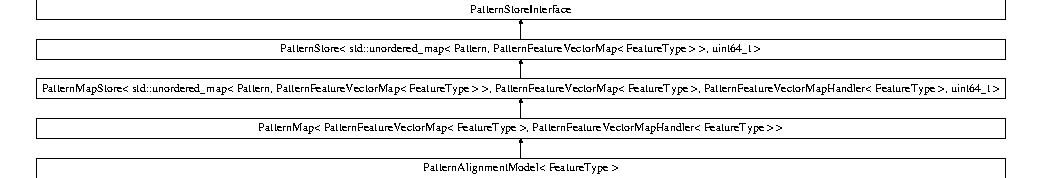
\includegraphics[height=2.300740cm]{classPatternAlignmentModel}
\end{center}
\end{figure}
\subsection*{Public Types}
\begin{DoxyCompactItemize}
\item 
typedef \hyperlink{classPatternMap}{Pattern\+Map}$<$ \hyperlink{classPatternFeatureVectorMap}{Pattern\+Feature\+Vector\+Map}$<$ Feature\+Type $>$, \hyperlink{classPatternFeatureVectorMapHandler}{Pattern\+Feature\+Vector\+Map\+Handler}$<$ Feature\+Type $>$ $>$\+::\hyperlink{classPatternAlignmentModel_a108db1926176ea0b761a8329fc73e3e7}{iterator} \hyperlink{classPatternAlignmentModel_a108db1926176ea0b761a8329fc73e3e7}{iterator}
\item 
typedef \hyperlink{classPatternMap}{Pattern\+Map}$<$ \hyperlink{classPatternFeatureVectorMap}{Pattern\+Feature\+Vector\+Map}$<$ Feature\+Type $>$, \hyperlink{classPatternFeatureVectorMapHandler}{Pattern\+Feature\+Vector\+Map\+Handler}$<$ Feature\+Type $>$ $>$\+::\hyperlink{classPatternAlignmentModel_ac8d8a6556af4672ceb0f29d7cfaa9db4}{const\+\_\+iterator} \hyperlink{classPatternAlignmentModel_ac8d8a6556af4672ceb0f29d7cfaa9db4}{const\+\_\+iterator}
\end{DoxyCompactItemize}
\subsection*{Public Member Functions}
\begin{DoxyCompactItemize}
\item 
\hyperlink{classPatternAlignmentModel_ae3bc572f6931c070eda7532f7f38cffb}{Pattern\+Alignment\+Model} ()
\item 
\hyperlink{classPatternAlignmentModel_a993125d3b974dc0b6a0687edf2351bfd}{Pattern\+Alignment\+Model} (std\+::istream $\ast$f, \hyperlink{classPatternModelOptions}{Pattern\+Model\+Options} options, \hyperlink{classPatternModelInterface}{Pattern\+Model\+Interface} $\ast$constrainmodel=N\+U\+L\+L)
\item 
\hyperlink{classPatternAlignmentModel_a345ff8a3e9d592c6b7621ee33dc44666}{Pattern\+Alignment\+Model} (const std\+::string filename, const \hyperlink{classPatternModelOptions}{Pattern\+Model\+Options} options, \hyperlink{classPatternModelInterface}{Pattern\+Model\+Interface} $\ast$constrainmodel=N\+U\+L\+L)
\item 
virtual int \hyperlink{classPatternAlignmentModel_a09c9e5d1d2287e1d751e0f70add38923}{getmodeltype} () const 
\item 
virtual int \hyperlink{classPatternAlignmentModel_adc7008d0dc96afc19d6b61ccde38c3c8}{getmodelversion} () const 
\item 
virtual size\+\_\+t \hyperlink{classPatternAlignmentModel_a7e4b2a69fd2e0852af0ed6ffaf6c51dc}{size} () const 
\item 
virtual bool \hyperlink{classPatternAlignmentModel_a4822a730be0dabeebd06771c803b8254}{has} (const \hyperlink{classPattern}{Pattern} \&pattern) const 
\item 
virtual bool \hyperlink{classPatternAlignmentModel_ad81e599091c476a9cb121e7e04a4da5a}{has} (const \hyperlink{classPatternPointer}{Pattern\+Pointer} \&pattern) const 
\item 
virtual void \hyperlink{classPatternAlignmentModel_af9d29f9bd63804ece43632b866042077}{load} (std\+::string filename, const \hyperlink{classPatternModelOptions}{Pattern\+Model\+Options} options, \hyperlink{classPatternModelInterface}{Pattern\+Model\+Interface} $\ast$constrainmodel=N\+U\+L\+L)
\item 
virtual void \hyperlink{classPatternAlignmentModel_a1ea66828aca73e774ad10985bc37fe8b}{load} (std\+::istream $\ast$f, \hyperlink{classPatternModelOptions}{Pattern\+Model\+Options} options, \hyperlink{classPatternModelInterface}{Pattern\+Model\+Interface} $\ast$constrainmodel=N\+U\+L\+L)
\item 
\hyperlink{classPatternModelInterface}{Pattern\+Model\+Interface} $\ast$ \hyperlink{classPatternAlignmentModel_aa3589420a199d86a117ca661ab4d5694}{getinterface} ()
\item 
void \hyperlink{classPatternAlignmentModel_a335c3f85686db801fafeb328bf8df5e8}{write} (std\+::ostream $\ast$out)
\item 
void \hyperlink{classPatternAlignmentModel_a9648856710033da53fa87f7fd52ddab1}{write} (const std\+::string filename)
\item 
virtual int \hyperlink{classPatternAlignmentModel_a304de9330665edddeadd418368165a4f}{maxlength} () const 
\item 
virtual int \hyperlink{classPatternAlignmentModel_a5ce5600308b9c985d4197853ec4f35a7}{minlength} () const 
\item 
virtual int \hyperlink{classPatternAlignmentModel_a98266fb6a4b062d35275737f34139440}{occurrencecount} (const \hyperlink{classPattern}{Pattern} \&pattern)
\item 
virtual \hyperlink{classPatternFeatureVectorMap}{Pattern\+Feature\+Vector\+Map}$<$ Feature\+Type $>$ $\ast$ \hyperlink{classPatternAlignmentModel_a320018e7e852d6428db5368a0c076a2d}{getdata} (const \hyperlink{classPattern}{Pattern} \&pattern, bool makeifnew=false)
\item 
virtual \hyperlink{classPatternFeatureVectorMap}{Pattern\+Feature\+Vector\+Map}$<$ Feature\+Type $>$ $\ast$ \hyperlink{classPatternAlignmentModel_a5f14f98332c38a211d12a9eddbc056da}{getdata} (const \hyperlink{classPatternPointer}{Pattern\+Pointer} \&patternpointer, bool makeifnew=false)
\item 
int \hyperlink{classPatternAlignmentModel_a4b7cea0a70074db5314d47b3768633cc}{types} () const 
\item 
int \hyperlink{classPatternAlignmentModel_a44a222ef3c195ac3eff61ae35bf84d77}{tokens} () const 
\item 
unsigned char \hyperlink{classPatternAlignmentModel_a4261323744204ec80057bb56ce34ffc1}{type} () const 
\item 
unsigned char \hyperlink{classPatternAlignmentModel_a7ca0fbfb5669d6fbfd7b24d11092074b}{version} () const 
\item 
virtual bool \hyperlink{classPatternAlignmentModel_a2617a747d23df9dfd0fd66aba9cbea6b}{has} (const \hyperlink{classPattern}{Pattern} \&pattern, const \hyperlink{classPattern}{Pattern} \&pattern2)
\item 
virtual bool \hyperlink{classPatternAlignmentModel_acfec49f2317d9dd12aebe630b6caa413}{has} (const \hyperlink{classPatternPointer}{Pattern\+Pointer} \&patternpointer, const \hyperlink{classPatternPointer}{Pattern\+Pointer} \&patternpointer2)
\item 
virtual \hyperlink{classPatternFeatureVector}{Pattern\+Feature\+Vector}$<$ Feature\+Type $>$ $\ast$ \hyperlink{classPatternAlignmentModel_a653ae7ceb0293d8928be37ab705d8a52}{getdata} (const \hyperlink{classPattern}{Pattern} \&pattern, const \hyperlink{classPattern}{Pattern} \&pattern2, bool makeifnew=false)
\item 
void \hyperlink{classPatternAlignmentModel_aa190384f055bf69a6ae4becb66651722}{add} (const \hyperlink{classPattern}{Pattern} \&pattern, const \hyperlink{classPattern}{Pattern} \&pattern2, std\+::vector$<$ Feature\+Type $>$ \&features, bool checkifexists=true)
\item 
virtual void \hyperlink{classPatternAlignmentModel_a0fe0e90c0a32fc35292f0b871f652084}{printmodel} (std\+::ostream $\ast$out, \hyperlink{classClassDecoder}{Class\+Decoder} \&sourcedecoder, \hyperlink{classClassDecoder}{Class\+Decoder} \&targetdecoder)
\item 
virtual void \hyperlink{classPatternAlignmentModel_a862fcfacc9903ba08ec4f134264c5da4}{print} (std\+::ostream $\ast$out, \hyperlink{classClassDecoder}{Class\+Decoder} \&sourcedecoder, \hyperlink{classClassDecoder}{Class\+Decoder} \&targetdecoder)
\end{DoxyCompactItemize}
\subsection*{Protected Member Functions}
\begin{DoxyCompactItemize}
\item 
virtual void \hyperlink{classPatternAlignmentModel_a84553b3366b622baad68f3d8c2e87675}{postread} (const \hyperlink{classPatternModelOptions}{Pattern\+Model\+Options} options)
\end{DoxyCompactItemize}
\subsection*{Protected Attributes}
\begin{DoxyCompactItemize}
\item 
unsigned char \hyperlink{classPatternAlignmentModel_a7f24c75a6674ae6bbe70b9fd36286562}{model\+\_\+type}
\item 
unsigned char \hyperlink{classPatternAlignmentModel_ae697eaef720c1ba038fe444b6a7eccd5}{model\+\_\+version}
\item 
uint64\+\_\+t \hyperlink{classPatternAlignmentModel_ad346131805c2e639a0e223db07ba869a}{totaltokens}
\item 
uint64\+\_\+t \hyperlink{classPatternAlignmentModel_a36279cac113c61b57f4a95df6e0a07b7}{totaltypes}
\item 
int \hyperlink{classPatternAlignmentModel_a6d7688c2dcff6c341e2b0b05fa242cb0}{maxn}
\item 
int \hyperlink{classPatternAlignmentModel_a9d844ce6aeb1956b8f7c36e9df05ea17}{minn}
\end{DoxyCompactItemize}


\subsection{Member Typedef Documentation}
\hypertarget{classPatternAlignmentModel_ac8d8a6556af4672ceb0f29d7cfaa9db4}{}\index{Pattern\+Alignment\+Model@{Pattern\+Alignment\+Model}!const\+\_\+iterator@{const\+\_\+iterator}}
\index{const\+\_\+iterator@{const\+\_\+iterator}!Pattern\+Alignment\+Model@{Pattern\+Alignment\+Model}}
\subsubsection[{const\+\_\+iterator}]{\setlength{\rightskip}{0pt plus 5cm}template$<$class Feature\+Type$>$ typedef {\bf Pattern\+Map}$<${\bf Pattern\+Feature\+Vector\+Map}$<$Feature\+Type$>$,{\bf Pattern\+Feature\+Vector\+Map\+Handler}$<$Feature\+Type$>$ $>$\+::{\bf const\+\_\+iterator} {\bf Pattern\+Alignment\+Model}$<$ Feature\+Type $>$\+::{\bf const\+\_\+iterator}}\label{classPatternAlignmentModel_ac8d8a6556af4672ceb0f29d7cfaa9db4}
\hypertarget{classPatternAlignmentModel_a108db1926176ea0b761a8329fc73e3e7}{}\index{Pattern\+Alignment\+Model@{Pattern\+Alignment\+Model}!iterator@{iterator}}
\index{iterator@{iterator}!Pattern\+Alignment\+Model@{Pattern\+Alignment\+Model}}
\subsubsection[{iterator}]{\setlength{\rightskip}{0pt plus 5cm}template$<$class Feature\+Type$>$ typedef {\bf Pattern\+Map}$<${\bf Pattern\+Feature\+Vector\+Map}$<$Feature\+Type$>$,{\bf Pattern\+Feature\+Vector\+Map\+Handler}$<$Feature\+Type$>$ $>$\+::{\bf iterator} {\bf Pattern\+Alignment\+Model}$<$ Feature\+Type $>$\+::{\bf iterator}}\label{classPatternAlignmentModel_a108db1926176ea0b761a8329fc73e3e7}


\subsection{Constructor \& Destructor Documentation}
\hypertarget{classPatternAlignmentModel_ae3bc572f6931c070eda7532f7f38cffb}{}\index{Pattern\+Alignment\+Model@{Pattern\+Alignment\+Model}!Pattern\+Alignment\+Model@{Pattern\+Alignment\+Model}}
\index{Pattern\+Alignment\+Model@{Pattern\+Alignment\+Model}!Pattern\+Alignment\+Model@{Pattern\+Alignment\+Model}}
\subsubsection[{Pattern\+Alignment\+Model()}]{\setlength{\rightskip}{0pt plus 5cm}template$<$class Feature\+Type$>$ {\bf Pattern\+Alignment\+Model}$<$ Feature\+Type $>$\+::{\bf Pattern\+Alignment\+Model} (
\begin{DoxyParamCaption}
{}
\end{DoxyParamCaption}
)\hspace{0.3cm}{\ttfamily [inline]}}\label{classPatternAlignmentModel_ae3bc572f6931c070eda7532f7f38cffb}
\hypertarget{classPatternAlignmentModel_a993125d3b974dc0b6a0687edf2351bfd}{}\index{Pattern\+Alignment\+Model@{Pattern\+Alignment\+Model}!Pattern\+Alignment\+Model@{Pattern\+Alignment\+Model}}
\index{Pattern\+Alignment\+Model@{Pattern\+Alignment\+Model}!Pattern\+Alignment\+Model@{Pattern\+Alignment\+Model}}
\subsubsection[{Pattern\+Alignment\+Model(std\+::istream $\ast$f, Pattern\+Model\+Options options, Pattern\+Model\+Interface $\ast$constrainmodel=\+N\+U\+L\+L)}]{\setlength{\rightskip}{0pt plus 5cm}template$<$class Feature\+Type$>$ {\bf Pattern\+Alignment\+Model}$<$ Feature\+Type $>$\+::{\bf Pattern\+Alignment\+Model} (
\begin{DoxyParamCaption}
\item[{std\+::istream $\ast$}]{f, }
\item[{{\bf Pattern\+Model\+Options}}]{options, }
\item[{{\bf Pattern\+Model\+Interface} $\ast$}]{constrainmodel = {\ttfamily NULL}}
\end{DoxyParamCaption}
)\hspace{0.3cm}{\ttfamily [inline]}}\label{classPatternAlignmentModel_a993125d3b974dc0b6a0687edf2351bfd}
\hypertarget{classPatternAlignmentModel_a345ff8a3e9d592c6b7621ee33dc44666}{}\index{Pattern\+Alignment\+Model@{Pattern\+Alignment\+Model}!Pattern\+Alignment\+Model@{Pattern\+Alignment\+Model}}
\index{Pattern\+Alignment\+Model@{Pattern\+Alignment\+Model}!Pattern\+Alignment\+Model@{Pattern\+Alignment\+Model}}
\subsubsection[{Pattern\+Alignment\+Model(const std\+::string filename, const Pattern\+Model\+Options options, Pattern\+Model\+Interface $\ast$constrainmodel=\+N\+U\+L\+L)}]{\setlength{\rightskip}{0pt plus 5cm}template$<$class Feature\+Type$>$ {\bf Pattern\+Alignment\+Model}$<$ Feature\+Type $>$\+::{\bf Pattern\+Alignment\+Model} (
\begin{DoxyParamCaption}
\item[{const std\+::string}]{filename, }
\item[{const {\bf Pattern\+Model\+Options}}]{options, }
\item[{{\bf Pattern\+Model\+Interface} $\ast$}]{constrainmodel = {\ttfamily NULL}}
\end{DoxyParamCaption}
)\hspace{0.3cm}{\ttfamily [inline]}}\label{classPatternAlignmentModel_a345ff8a3e9d592c6b7621ee33dc44666}


\subsection{Member Function Documentation}
\hypertarget{classPatternAlignmentModel_aa190384f055bf69a6ae4becb66651722}{}\index{Pattern\+Alignment\+Model@{Pattern\+Alignment\+Model}!add@{add}}
\index{add@{add}!Pattern\+Alignment\+Model@{Pattern\+Alignment\+Model}}
\subsubsection[{add(const Pattern \&pattern, const Pattern \&pattern2, std\+::vector$<$ Feature\+Type $>$ \&features, bool checkifexists=true)}]{\setlength{\rightskip}{0pt plus 5cm}template$<$class Feature\+Type$>$ void {\bf Pattern\+Alignment\+Model}$<$ Feature\+Type $>$\+::add (
\begin{DoxyParamCaption}
\item[{const {\bf Pattern} \&}]{pattern, }
\item[{const {\bf Pattern} \&}]{pattern2, }
\item[{std\+::vector$<$ Feature\+Type $>$ \&}]{features, }
\item[{bool}]{checkifexists = {\ttfamily true}}
\end{DoxyParamCaption}
)\hspace{0.3cm}{\ttfamily [inline]}}\label{classPatternAlignmentModel_aa190384f055bf69a6ae4becb66651722}
\hypertarget{classPatternAlignmentModel_a320018e7e852d6428db5368a0c076a2d}{}\index{Pattern\+Alignment\+Model@{Pattern\+Alignment\+Model}!getdata@{getdata}}
\index{getdata@{getdata}!Pattern\+Alignment\+Model@{Pattern\+Alignment\+Model}}
\subsubsection[{getdata(const Pattern \&pattern, bool makeifnew=false)}]{\setlength{\rightskip}{0pt plus 5cm}template$<$class Feature\+Type$>$ virtual {\bf Pattern\+Feature\+Vector\+Map}$<$Feature\+Type$>$$\ast$ {\bf Pattern\+Alignment\+Model}$<$ Feature\+Type $>$\+::getdata (
\begin{DoxyParamCaption}
\item[{const {\bf Pattern} \&}]{pattern, }
\item[{bool}]{makeifnew = {\ttfamily false}}
\end{DoxyParamCaption}
)\hspace{0.3cm}{\ttfamily [inline]}, {\ttfamily [virtual]}}\label{classPatternAlignmentModel_a320018e7e852d6428db5368a0c076a2d}
\hypertarget{classPatternAlignmentModel_a5f14f98332c38a211d12a9eddbc056da}{}\index{Pattern\+Alignment\+Model@{Pattern\+Alignment\+Model}!getdata@{getdata}}
\index{getdata@{getdata}!Pattern\+Alignment\+Model@{Pattern\+Alignment\+Model}}
\subsubsection[{getdata(const Pattern\+Pointer \&patternpointer, bool makeifnew=false)}]{\setlength{\rightskip}{0pt plus 5cm}template$<$class Feature\+Type$>$ virtual {\bf Pattern\+Feature\+Vector\+Map}$<$Feature\+Type$>$$\ast$ {\bf Pattern\+Alignment\+Model}$<$ Feature\+Type $>$\+::getdata (
\begin{DoxyParamCaption}
\item[{const {\bf Pattern\+Pointer} \&}]{patternpointer, }
\item[{bool}]{makeifnew = {\ttfamily false}}
\end{DoxyParamCaption}
)\hspace{0.3cm}{\ttfamily [inline]}, {\ttfamily [virtual]}}\label{classPatternAlignmentModel_a5f14f98332c38a211d12a9eddbc056da}
\hypertarget{classPatternAlignmentModel_a653ae7ceb0293d8928be37ab705d8a52}{}\index{Pattern\+Alignment\+Model@{Pattern\+Alignment\+Model}!getdata@{getdata}}
\index{getdata@{getdata}!Pattern\+Alignment\+Model@{Pattern\+Alignment\+Model}}
\subsubsection[{getdata(const Pattern \&pattern, const Pattern \&pattern2, bool makeifnew=false)}]{\setlength{\rightskip}{0pt plus 5cm}template$<$class Feature\+Type$>$ virtual {\bf Pattern\+Feature\+Vector}$<$Feature\+Type$>$$\ast$ {\bf Pattern\+Alignment\+Model}$<$ Feature\+Type $>$\+::getdata (
\begin{DoxyParamCaption}
\item[{const {\bf Pattern} \&}]{pattern, }
\item[{const {\bf Pattern} \&}]{pattern2, }
\item[{bool}]{makeifnew = {\ttfamily false}}
\end{DoxyParamCaption}
)\hspace{0.3cm}{\ttfamily [inline]}, {\ttfamily [virtual]}}\label{classPatternAlignmentModel_a653ae7ceb0293d8928be37ab705d8a52}
\hypertarget{classPatternAlignmentModel_aa3589420a199d86a117ca661ab4d5694}{}\index{Pattern\+Alignment\+Model@{Pattern\+Alignment\+Model}!getinterface@{getinterface}}
\index{getinterface@{getinterface}!Pattern\+Alignment\+Model@{Pattern\+Alignment\+Model}}
\subsubsection[{getinterface()}]{\setlength{\rightskip}{0pt plus 5cm}template$<$class Feature\+Type$>$ {\bf Pattern\+Model\+Interface}$\ast$ {\bf Pattern\+Alignment\+Model}$<$ Feature\+Type $>$\+::getinterface (
\begin{DoxyParamCaption}
{}
\end{DoxyParamCaption}
)\hspace{0.3cm}{\ttfamily [inline]}}\label{classPatternAlignmentModel_aa3589420a199d86a117ca661ab4d5694}
\hypertarget{classPatternAlignmentModel_a09c9e5d1d2287e1d751e0f70add38923}{}\index{Pattern\+Alignment\+Model@{Pattern\+Alignment\+Model}!getmodeltype@{getmodeltype}}
\index{getmodeltype@{getmodeltype}!Pattern\+Alignment\+Model@{Pattern\+Alignment\+Model}}
\subsubsection[{getmodeltype() const }]{\setlength{\rightskip}{0pt plus 5cm}template$<$class Feature\+Type$>$ virtual int {\bf Pattern\+Alignment\+Model}$<$ Feature\+Type $>$\+::getmodeltype (
\begin{DoxyParamCaption}
{}
\end{DoxyParamCaption}
) const\hspace{0.3cm}{\ttfamily [inline]}, {\ttfamily [virtual]}}\label{classPatternAlignmentModel_a09c9e5d1d2287e1d751e0f70add38923}
\hypertarget{classPatternAlignmentModel_adc7008d0dc96afc19d6b61ccde38c3c8}{}\index{Pattern\+Alignment\+Model@{Pattern\+Alignment\+Model}!getmodelversion@{getmodelversion}}
\index{getmodelversion@{getmodelversion}!Pattern\+Alignment\+Model@{Pattern\+Alignment\+Model}}
\subsubsection[{getmodelversion() const }]{\setlength{\rightskip}{0pt plus 5cm}template$<$class Feature\+Type$>$ virtual int {\bf Pattern\+Alignment\+Model}$<$ Feature\+Type $>$\+::getmodelversion (
\begin{DoxyParamCaption}
{}
\end{DoxyParamCaption}
) const\hspace{0.3cm}{\ttfamily [inline]}, {\ttfamily [virtual]}}\label{classPatternAlignmentModel_adc7008d0dc96afc19d6b61ccde38c3c8}
\hypertarget{classPatternAlignmentModel_a4822a730be0dabeebd06771c803b8254}{}\index{Pattern\+Alignment\+Model@{Pattern\+Alignment\+Model}!has@{has}}
\index{has@{has}!Pattern\+Alignment\+Model@{Pattern\+Alignment\+Model}}
\subsubsection[{has(const Pattern \&pattern) const }]{\setlength{\rightskip}{0pt plus 5cm}template$<$class Feature\+Type$>$ virtual bool {\bf Pattern\+Alignment\+Model}$<$ Feature\+Type $>$\+::has (
\begin{DoxyParamCaption}
\item[{const {\bf Pattern} \&}]{}
\end{DoxyParamCaption}
) const\hspace{0.3cm}{\ttfamily [inline]}, {\ttfamily [virtual]}}\label{classPatternAlignmentModel_a4822a730be0dabeebd06771c803b8254}
Does the pattern occur in the pattern store? 

Implements \hyperlink{classPatternMapStore_a208cf2d90725a3a9291d2dae67ac9256}{Pattern\+Map\+Store$<$ std\+::unordered\+\_\+map$<$ Pattern, Pattern\+Feature\+Vector\+Map$<$ Feature\+Type $>$ $>$, Pattern\+Feature\+Vector\+Map$<$ Feature\+Type $>$, Pattern\+Feature\+Vector\+Map\+Handler$<$ Feature\+Type $>$, uint64\+\_\+t, Pattern $>$}.

\hypertarget{classPatternAlignmentModel_ad81e599091c476a9cb121e7e04a4da5a}{}\index{Pattern\+Alignment\+Model@{Pattern\+Alignment\+Model}!has@{has}}
\index{has@{has}!Pattern\+Alignment\+Model@{Pattern\+Alignment\+Model}}
\subsubsection[{has(const Pattern\+Pointer \&pattern) const }]{\setlength{\rightskip}{0pt plus 5cm}template$<$class Feature\+Type$>$ virtual bool {\bf Pattern\+Alignment\+Model}$<$ Feature\+Type $>$\+::has (
\begin{DoxyParamCaption}
\item[{const {\bf Pattern\+Pointer} \&}]{}
\end{DoxyParamCaption}
) const\hspace{0.3cm}{\ttfamily [inline]}, {\ttfamily [virtual]}}\label{classPatternAlignmentModel_ad81e599091c476a9cb121e7e04a4da5a}
Does the pattern occur in the pattern store? 

Implements \hyperlink{classPatternMapStore_a4bce03112ff9c3c0950f31ccee0c9ab8}{Pattern\+Map\+Store$<$ std\+::unordered\+\_\+map$<$ Pattern, Pattern\+Feature\+Vector\+Map$<$ Feature\+Type $>$ $>$, Pattern\+Feature\+Vector\+Map$<$ Feature\+Type $>$, Pattern\+Feature\+Vector\+Map\+Handler$<$ Feature\+Type $>$, uint64\+\_\+t, Pattern $>$}.

\hypertarget{classPatternAlignmentModel_a2617a747d23df9dfd0fd66aba9cbea6b}{}\index{Pattern\+Alignment\+Model@{Pattern\+Alignment\+Model}!has@{has}}
\index{has@{has}!Pattern\+Alignment\+Model@{Pattern\+Alignment\+Model}}
\subsubsection[{has(const Pattern \&pattern, const Pattern \&pattern2)}]{\setlength{\rightskip}{0pt plus 5cm}template$<$class Feature\+Type$>$ virtual bool {\bf Pattern\+Alignment\+Model}$<$ Feature\+Type $>$\+::has (
\begin{DoxyParamCaption}
\item[{const {\bf Pattern} \&}]{pattern, }
\item[{const {\bf Pattern} \&}]{pattern2}
\end{DoxyParamCaption}
)\hspace{0.3cm}{\ttfamily [inline]}, {\ttfamily [virtual]}}\label{classPatternAlignmentModel_a2617a747d23df9dfd0fd66aba9cbea6b}
\hypertarget{classPatternAlignmentModel_acfec49f2317d9dd12aebe630b6caa413}{}\index{Pattern\+Alignment\+Model@{Pattern\+Alignment\+Model}!has@{has}}
\index{has@{has}!Pattern\+Alignment\+Model@{Pattern\+Alignment\+Model}}
\subsubsection[{has(const Pattern\+Pointer \&patternpointer, const Pattern\+Pointer \&patternpointer2)}]{\setlength{\rightskip}{0pt plus 5cm}template$<$class Feature\+Type$>$ virtual bool {\bf Pattern\+Alignment\+Model}$<$ Feature\+Type $>$\+::has (
\begin{DoxyParamCaption}
\item[{const {\bf Pattern\+Pointer} \&}]{patternpointer, }
\item[{const {\bf Pattern\+Pointer} \&}]{patternpointer2}
\end{DoxyParamCaption}
)\hspace{0.3cm}{\ttfamily [inline]}, {\ttfamily [virtual]}}\label{classPatternAlignmentModel_acfec49f2317d9dd12aebe630b6caa413}
\hypertarget{classPatternAlignmentModel_af9d29f9bd63804ece43632b866042077}{}\index{Pattern\+Alignment\+Model@{Pattern\+Alignment\+Model}!load@{load}}
\index{load@{load}!Pattern\+Alignment\+Model@{Pattern\+Alignment\+Model}}
\subsubsection[{load(std\+::string filename, const Pattern\+Model\+Options options, Pattern\+Model\+Interface $\ast$constrainmodel=\+N\+U\+L\+L)}]{\setlength{\rightskip}{0pt plus 5cm}template$<$class Feature\+Type$>$ virtual void {\bf Pattern\+Alignment\+Model}$<$ Feature\+Type $>$\+::load (
\begin{DoxyParamCaption}
\item[{std\+::string}]{filename, }
\item[{const {\bf Pattern\+Model\+Options}}]{options, }
\item[{{\bf Pattern\+Model\+Interface} $\ast$}]{constrainmodel = {\ttfamily NULL}}
\end{DoxyParamCaption}
)\hspace{0.3cm}{\ttfamily [inline]}, {\ttfamily [virtual]}}\label{classPatternAlignmentModel_af9d29f9bd63804ece43632b866042077}
\hypertarget{classPatternAlignmentModel_a1ea66828aca73e774ad10985bc37fe8b}{}\index{Pattern\+Alignment\+Model@{Pattern\+Alignment\+Model}!load@{load}}
\index{load@{load}!Pattern\+Alignment\+Model@{Pattern\+Alignment\+Model}}
\subsubsection[{load(std\+::istream $\ast$f, Pattern\+Model\+Options options, Pattern\+Model\+Interface $\ast$constrainmodel=\+N\+U\+L\+L)}]{\setlength{\rightskip}{0pt plus 5cm}template$<$class Feature\+Type$>$ virtual void {\bf Pattern\+Alignment\+Model}$<$ Feature\+Type $>$\+::load (
\begin{DoxyParamCaption}
\item[{std\+::istream $\ast$}]{f, }
\item[{{\bf Pattern\+Model\+Options}}]{options, }
\item[{{\bf Pattern\+Model\+Interface} $\ast$}]{constrainmodel = {\ttfamily NULL}}
\end{DoxyParamCaption}
)\hspace{0.3cm}{\ttfamily [inline]}, {\ttfamily [virtual]}}\label{classPatternAlignmentModel_a1ea66828aca73e774ad10985bc37fe8b}
\hypertarget{classPatternAlignmentModel_a304de9330665edddeadd418368165a4f}{}\index{Pattern\+Alignment\+Model@{Pattern\+Alignment\+Model}!maxlength@{maxlength}}
\index{maxlength@{maxlength}!Pattern\+Alignment\+Model@{Pattern\+Alignment\+Model}}
\subsubsection[{maxlength() const }]{\setlength{\rightskip}{0pt plus 5cm}template$<$class Feature\+Type$>$ virtual int {\bf Pattern\+Alignment\+Model}$<$ Feature\+Type $>$\+::maxlength (
\begin{DoxyParamCaption}
{}
\end{DoxyParamCaption}
) const\hspace{0.3cm}{\ttfamily [inline]}, {\ttfamily [virtual]}}\label{classPatternAlignmentModel_a304de9330665edddeadd418368165a4f}
\hypertarget{classPatternAlignmentModel_a5ce5600308b9c985d4197853ec4f35a7}{}\index{Pattern\+Alignment\+Model@{Pattern\+Alignment\+Model}!minlength@{minlength}}
\index{minlength@{minlength}!Pattern\+Alignment\+Model@{Pattern\+Alignment\+Model}}
\subsubsection[{minlength() const }]{\setlength{\rightskip}{0pt plus 5cm}template$<$class Feature\+Type$>$ virtual int {\bf Pattern\+Alignment\+Model}$<$ Feature\+Type $>$\+::minlength (
\begin{DoxyParamCaption}
{}
\end{DoxyParamCaption}
) const\hspace{0.3cm}{\ttfamily [inline]}, {\ttfamily [virtual]}}\label{classPatternAlignmentModel_a5ce5600308b9c985d4197853ec4f35a7}
\hypertarget{classPatternAlignmentModel_a98266fb6a4b062d35275737f34139440}{}\index{Pattern\+Alignment\+Model@{Pattern\+Alignment\+Model}!occurrencecount@{occurrencecount}}
\index{occurrencecount@{occurrencecount}!Pattern\+Alignment\+Model@{Pattern\+Alignment\+Model}}
\subsubsection[{occurrencecount(const Pattern \&pattern)}]{\setlength{\rightskip}{0pt plus 5cm}template$<$class Feature\+Type$>$ virtual int {\bf Pattern\+Alignment\+Model}$<$ Feature\+Type $>$\+::occurrencecount (
\begin{DoxyParamCaption}
\item[{const {\bf Pattern} \&}]{pattern}
\end{DoxyParamCaption}
)\hspace{0.3cm}{\ttfamily [inline]}, {\ttfamily [virtual]}}\label{classPatternAlignmentModel_a98266fb6a4b062d35275737f34139440}
\hypertarget{classPatternAlignmentModel_a84553b3366b622baad68f3d8c2e87675}{}\index{Pattern\+Alignment\+Model@{Pattern\+Alignment\+Model}!postread@{postread}}
\index{postread@{postread}!Pattern\+Alignment\+Model@{Pattern\+Alignment\+Model}}
\subsubsection[{postread(const Pattern\+Model\+Options options)}]{\setlength{\rightskip}{0pt plus 5cm}template$<$class Feature\+Type$>$ virtual void {\bf Pattern\+Alignment\+Model}$<$ Feature\+Type $>$\+::postread (
\begin{DoxyParamCaption}
\item[{const {\bf Pattern\+Model\+Options}}]{options}
\end{DoxyParamCaption}
)\hspace{0.3cm}{\ttfamily [inline]}, {\ttfamily [protected]}, {\ttfamily [virtual]}}\label{classPatternAlignmentModel_a84553b3366b622baad68f3d8c2e87675}
\hypertarget{classPatternAlignmentModel_a862fcfacc9903ba08ec4f134264c5da4}{}\index{Pattern\+Alignment\+Model@{Pattern\+Alignment\+Model}!print@{print}}
\index{print@{print}!Pattern\+Alignment\+Model@{Pattern\+Alignment\+Model}}
\subsubsection[{print(std\+::ostream $\ast$out, Class\+Decoder \&sourcedecoder, Class\+Decoder \&targetdecoder)}]{\setlength{\rightskip}{0pt plus 5cm}template$<$class Feature\+Type$>$ virtual void {\bf Pattern\+Alignment\+Model}$<$ Feature\+Type $>$\+::print (
\begin{DoxyParamCaption}
\item[{std\+::ostream $\ast$}]{out, }
\item[{{\bf Class\+Decoder} \&}]{sourcedecoder, }
\item[{{\bf Class\+Decoder} \&}]{targetdecoder}
\end{DoxyParamCaption}
)\hspace{0.3cm}{\ttfamily [inline]}, {\ttfamily [virtual]}}\label{classPatternAlignmentModel_a862fcfacc9903ba08ec4f134264c5da4}
\hypertarget{classPatternAlignmentModel_a0fe0e90c0a32fc35292f0b871f652084}{}\index{Pattern\+Alignment\+Model@{Pattern\+Alignment\+Model}!printmodel@{printmodel}}
\index{printmodel@{printmodel}!Pattern\+Alignment\+Model@{Pattern\+Alignment\+Model}}
\subsubsection[{printmodel(std\+::ostream $\ast$out, Class\+Decoder \&sourcedecoder, Class\+Decoder \&targetdecoder)}]{\setlength{\rightskip}{0pt plus 5cm}template$<$class Feature\+Type$>$ virtual void {\bf Pattern\+Alignment\+Model}$<$ Feature\+Type $>$\+::printmodel (
\begin{DoxyParamCaption}
\item[{std\+::ostream $\ast$}]{out, }
\item[{{\bf Class\+Decoder} \&}]{sourcedecoder, }
\item[{{\bf Class\+Decoder} \&}]{targetdecoder}
\end{DoxyParamCaption}
)\hspace{0.3cm}{\ttfamily [inline]}, {\ttfamily [virtual]}}\label{classPatternAlignmentModel_a0fe0e90c0a32fc35292f0b871f652084}
\hypertarget{classPatternAlignmentModel_a7e4b2a69fd2e0852af0ed6ffaf6c51dc}{}\index{Pattern\+Alignment\+Model@{Pattern\+Alignment\+Model}!size@{size}}
\index{size@{size}!Pattern\+Alignment\+Model@{Pattern\+Alignment\+Model}}
\subsubsection[{size() const }]{\setlength{\rightskip}{0pt plus 5cm}template$<$class Feature\+Type$>$ virtual size\+\_\+t {\bf Pattern\+Alignment\+Model}$<$ Feature\+Type $>$\+::size (
\begin{DoxyParamCaption}
{}
\end{DoxyParamCaption}
) const\hspace{0.3cm}{\ttfamily [inline]}, {\ttfamily [virtual]}}\label{classPatternAlignmentModel_a7e4b2a69fd2e0852af0ed6ffaf6c51dc}
How many patterns are in the pattern store? 

Implements \hyperlink{classPatternMapStore_af7bd333e776a4e55af9add5ee320dbb5}{Pattern\+Map\+Store$<$ std\+::unordered\+\_\+map$<$ Pattern, Pattern\+Feature\+Vector\+Map$<$ Feature\+Type $>$ $>$, Pattern\+Feature\+Vector\+Map$<$ Feature\+Type $>$, Pattern\+Feature\+Vector\+Map\+Handler$<$ Feature\+Type $>$, uint64\+\_\+t, Pattern $>$}.

\hypertarget{classPatternAlignmentModel_a44a222ef3c195ac3eff61ae35bf84d77}{}\index{Pattern\+Alignment\+Model@{Pattern\+Alignment\+Model}!tokens@{tokens}}
\index{tokens@{tokens}!Pattern\+Alignment\+Model@{Pattern\+Alignment\+Model}}
\subsubsection[{tokens() const }]{\setlength{\rightskip}{0pt plus 5cm}template$<$class Feature\+Type$>$ int {\bf Pattern\+Alignment\+Model}$<$ Feature\+Type $>$\+::tokens (
\begin{DoxyParamCaption}
{}
\end{DoxyParamCaption}
) const\hspace{0.3cm}{\ttfamily [inline]}}\label{classPatternAlignmentModel_a44a222ef3c195ac3eff61ae35bf84d77}
\hypertarget{classPatternAlignmentModel_a4261323744204ec80057bb56ce34ffc1}{}\index{Pattern\+Alignment\+Model@{Pattern\+Alignment\+Model}!type@{type}}
\index{type@{type}!Pattern\+Alignment\+Model@{Pattern\+Alignment\+Model}}
\subsubsection[{type() const }]{\setlength{\rightskip}{0pt plus 5cm}template$<$class Feature\+Type$>$ unsigned char {\bf Pattern\+Alignment\+Model}$<$ Feature\+Type $>$\+::type (
\begin{DoxyParamCaption}
{}
\end{DoxyParamCaption}
) const\hspace{0.3cm}{\ttfamily [inline]}}\label{classPatternAlignmentModel_a4261323744204ec80057bb56ce34ffc1}
\hypertarget{classPatternAlignmentModel_a4b7cea0a70074db5314d47b3768633cc}{}\index{Pattern\+Alignment\+Model@{Pattern\+Alignment\+Model}!types@{types}}
\index{types@{types}!Pattern\+Alignment\+Model@{Pattern\+Alignment\+Model}}
\subsubsection[{types() const }]{\setlength{\rightskip}{0pt plus 5cm}template$<$class Feature\+Type$>$ int {\bf Pattern\+Alignment\+Model}$<$ Feature\+Type $>$\+::types (
\begin{DoxyParamCaption}
{}
\end{DoxyParamCaption}
) const\hspace{0.3cm}{\ttfamily [inline]}}\label{classPatternAlignmentModel_a4b7cea0a70074db5314d47b3768633cc}
\hypertarget{classPatternAlignmentModel_a7ca0fbfb5669d6fbfd7b24d11092074b}{}\index{Pattern\+Alignment\+Model@{Pattern\+Alignment\+Model}!version@{version}}
\index{version@{version}!Pattern\+Alignment\+Model@{Pattern\+Alignment\+Model}}
\subsubsection[{version() const }]{\setlength{\rightskip}{0pt plus 5cm}template$<$class Feature\+Type$>$ unsigned char {\bf Pattern\+Alignment\+Model}$<$ Feature\+Type $>$\+::version (
\begin{DoxyParamCaption}
{}
\end{DoxyParamCaption}
) const\hspace{0.3cm}{\ttfamily [inline]}}\label{classPatternAlignmentModel_a7ca0fbfb5669d6fbfd7b24d11092074b}
\hypertarget{classPatternAlignmentModel_a335c3f85686db801fafeb328bf8df5e8}{}\index{Pattern\+Alignment\+Model@{Pattern\+Alignment\+Model}!write@{write}}
\index{write@{write}!Pattern\+Alignment\+Model@{Pattern\+Alignment\+Model}}
\subsubsection[{write(std\+::ostream $\ast$out)}]{\setlength{\rightskip}{0pt plus 5cm}template$<$class Feature\+Type$>$ void {\bf Pattern\+Alignment\+Model}$<$ Feature\+Type $>$\+::write (
\begin{DoxyParamCaption}
\item[{std\+::ostream $\ast$}]{out}
\end{DoxyParamCaption}
)\hspace{0.3cm}{\ttfamily [inline]}, {\ttfamily [virtual]}}\label{classPatternAlignmentModel_a335c3f85686db801fafeb328bf8df5e8}
Write the map to stream output (in binary format) 

Reimplemented from \hyperlink{classPatternMapStore_aa6400b6ff29f93c3e1c73355363c2476}{Pattern\+Map\+Store$<$ std\+::unordered\+\_\+map$<$ Pattern, Pattern\+Feature\+Vector\+Map$<$ Feature\+Type $>$ $>$, Pattern\+Feature\+Vector\+Map$<$ Feature\+Type $>$, Pattern\+Feature\+Vector\+Map\+Handler$<$ Feature\+Type $>$, uint64\+\_\+t, Pattern $>$}.

\hypertarget{classPatternAlignmentModel_a9648856710033da53fa87f7fd52ddab1}{}\index{Pattern\+Alignment\+Model@{Pattern\+Alignment\+Model}!write@{write}}
\index{write@{write}!Pattern\+Alignment\+Model@{Pattern\+Alignment\+Model}}
\subsubsection[{write(const std\+::string filename)}]{\setlength{\rightskip}{0pt plus 5cm}template$<$class Feature\+Type$>$ void {\bf Pattern\+Alignment\+Model}$<$ Feature\+Type $>$\+::write (
\begin{DoxyParamCaption}
\item[{const std\+::string}]{filename}
\end{DoxyParamCaption}
)\hspace{0.3cm}{\ttfamily [inline]}, {\ttfamily [virtual]}}\label{classPatternAlignmentModel_a9648856710033da53fa87f7fd52ddab1}
Write the map to file (in binary format) 

Reimplemented from \hyperlink{classPatternMapStore_a42c82c250e9a070d148637f7f7966c12}{Pattern\+Map\+Store$<$ std\+::unordered\+\_\+map$<$ Pattern, Pattern\+Feature\+Vector\+Map$<$ Feature\+Type $>$ $>$, Pattern\+Feature\+Vector\+Map$<$ Feature\+Type $>$, Pattern\+Feature\+Vector\+Map\+Handler$<$ Feature\+Type $>$, uint64\+\_\+t, Pattern $>$}.



\subsection{Member Data Documentation}
\hypertarget{classPatternAlignmentModel_a6d7688c2dcff6c341e2b0b05fa242cb0}{}\index{Pattern\+Alignment\+Model@{Pattern\+Alignment\+Model}!maxn@{maxn}}
\index{maxn@{maxn}!Pattern\+Alignment\+Model@{Pattern\+Alignment\+Model}}
\subsubsection[{maxn}]{\setlength{\rightskip}{0pt plus 5cm}template$<$class Feature\+Type$>$ int {\bf Pattern\+Alignment\+Model}$<$ Feature\+Type $>$\+::maxn\hspace{0.3cm}{\ttfamily [protected]}}\label{classPatternAlignmentModel_a6d7688c2dcff6c341e2b0b05fa242cb0}
\hypertarget{classPatternAlignmentModel_a9d844ce6aeb1956b8f7c36e9df05ea17}{}\index{Pattern\+Alignment\+Model@{Pattern\+Alignment\+Model}!minn@{minn}}
\index{minn@{minn}!Pattern\+Alignment\+Model@{Pattern\+Alignment\+Model}}
\subsubsection[{minn}]{\setlength{\rightskip}{0pt plus 5cm}template$<$class Feature\+Type$>$ int {\bf Pattern\+Alignment\+Model}$<$ Feature\+Type $>$\+::minn\hspace{0.3cm}{\ttfamily [protected]}}\label{classPatternAlignmentModel_a9d844ce6aeb1956b8f7c36e9df05ea17}
\hypertarget{classPatternAlignmentModel_a7f24c75a6674ae6bbe70b9fd36286562}{}\index{Pattern\+Alignment\+Model@{Pattern\+Alignment\+Model}!model\+\_\+type@{model\+\_\+type}}
\index{model\+\_\+type@{model\+\_\+type}!Pattern\+Alignment\+Model@{Pattern\+Alignment\+Model}}
\subsubsection[{model\+\_\+type}]{\setlength{\rightskip}{0pt plus 5cm}template$<$class Feature\+Type$>$ unsigned char {\bf Pattern\+Alignment\+Model}$<$ Feature\+Type $>$\+::model\+\_\+type\hspace{0.3cm}{\ttfamily [protected]}}\label{classPatternAlignmentModel_a7f24c75a6674ae6bbe70b9fd36286562}
\hypertarget{classPatternAlignmentModel_ae697eaef720c1ba038fe444b6a7eccd5}{}\index{Pattern\+Alignment\+Model@{Pattern\+Alignment\+Model}!model\+\_\+version@{model\+\_\+version}}
\index{model\+\_\+version@{model\+\_\+version}!Pattern\+Alignment\+Model@{Pattern\+Alignment\+Model}}
\subsubsection[{model\+\_\+version}]{\setlength{\rightskip}{0pt plus 5cm}template$<$class Feature\+Type$>$ unsigned char {\bf Pattern\+Alignment\+Model}$<$ Feature\+Type $>$\+::model\+\_\+version\hspace{0.3cm}{\ttfamily [protected]}}\label{classPatternAlignmentModel_ae697eaef720c1ba038fe444b6a7eccd5}
\hypertarget{classPatternAlignmentModel_ad346131805c2e639a0e223db07ba869a}{}\index{Pattern\+Alignment\+Model@{Pattern\+Alignment\+Model}!totaltokens@{totaltokens}}
\index{totaltokens@{totaltokens}!Pattern\+Alignment\+Model@{Pattern\+Alignment\+Model}}
\subsubsection[{totaltokens}]{\setlength{\rightskip}{0pt plus 5cm}template$<$class Feature\+Type$>$ uint64\+\_\+t {\bf Pattern\+Alignment\+Model}$<$ Feature\+Type $>$\+::totaltokens\hspace{0.3cm}{\ttfamily [protected]}}\label{classPatternAlignmentModel_ad346131805c2e639a0e223db07ba869a}
\hypertarget{classPatternAlignmentModel_a36279cac113c61b57f4a95df6e0a07b7}{}\index{Pattern\+Alignment\+Model@{Pattern\+Alignment\+Model}!totaltypes@{totaltypes}}
\index{totaltypes@{totaltypes}!Pattern\+Alignment\+Model@{Pattern\+Alignment\+Model}}
\subsubsection[{totaltypes}]{\setlength{\rightskip}{0pt plus 5cm}template$<$class Feature\+Type$>$ uint64\+\_\+t {\bf Pattern\+Alignment\+Model}$<$ Feature\+Type $>$\+::totaltypes\hspace{0.3cm}{\ttfamily [protected]}}\label{classPatternAlignmentModel_a36279cac113c61b57f4a95df6e0a07b7}


The documentation for this class was generated from the following file\+:\begin{DoxyCompactItemize}
\item 
include/\hyperlink{alignmodel_8h}{alignmodel.\+h}\end{DoxyCompactItemize}

\hypertarget{classPatternFeatureVector}{}\section{Pattern\+Feature\+Vector$<$ Feature\+Type $>$ Class Template Reference}
\label{classPatternFeatureVector}\index{Pattern\+Feature\+Vector$<$ Feature\+Type $>$@{Pattern\+Feature\+Vector$<$ Feature\+Type $>$}}


{\ttfamily \#include $<$datatypes.\+h$>$}

\subsection*{Public Types}
\begin{DoxyCompactItemize}
\item 
typedef std\+::vector$<$ Feature\+Type $>$\+::\hyperlink{classPatternFeatureVector_a4a2652f25b1f733630a6d1b8479fce77}{iterator} \hyperlink{classPatternFeatureVector_a4a2652f25b1f733630a6d1b8479fce77}{iterator}
\item 
typedef std\+::vector$<$ Feature\+Type $>$\+::\hyperlink{classPatternFeatureVector_a8fae8bc79a755c241964080a684cfd43}{const\+\_\+iterator} \hyperlink{classPatternFeatureVector_a8fae8bc79a755c241964080a684cfd43}{const\+\_\+iterator}
\end{DoxyCompactItemize}
\subsection*{Public Member Functions}
\begin{DoxyCompactItemize}
\item 
\hyperlink{classPatternFeatureVector_ad99d4a05d82fcf345432dff0b28306f0}{Pattern\+Feature\+Vector} ()
\item 
virtual \hyperlink{classPatternFeatureVector_a28391cd22ee11edf557e0f4c51df3f5b}{$\sim$\+Pattern\+Feature\+Vector} ()
\item 
\hyperlink{classPatternFeatureVector_a984df156b0fbf3a0a11bc1e57bea24a3}{Pattern\+Feature\+Vector} (const \hyperlink{classPattern}{Pattern} \&ref)
\item 
\hyperlink{classPatternFeatureVector_a7f6948af69865125ead89fa3ee3c83eb}{Pattern\+Feature\+Vector} (const \hyperlink{classPattern}{Pattern} \&ref, const std\+::vector$<$ Feature\+Type $>$ \&dataref)
\item 
\hyperlink{classPatternFeatureVector_a941dcf7305fb15d06ccd7c32690bc025}{Pattern\+Feature\+Vector} (const \hyperlink{classPatternFeatureVector}{Pattern\+Feature\+Vector} \&ref)
\item 
\hyperlink{classPatternFeatureVector_a2ce1bdcf182b806bd3e06e5c412221b4}{Pattern\+Feature\+Vector} (std\+::istream $\ast$in)
\item 
void \hyperlink{classPatternFeatureVector_a874b73d43566d1514404f9d8f1e7dd91}{read} (std\+::istream $\ast$in)
\item 
void \hyperlink{classPatternFeatureVector_ae315b88a17a31d7c79615c8cf17f2a6a}{write} (std\+::ostream $\ast$out)
\item 
size\+\_\+t \hyperlink{classPatternFeatureVector_ad99cf7876fda7bf9d7d41c8f0648df80}{size} () const 
\item 
\hyperlink{classPatternFeatureVector}{Pattern\+Feature\+Vector}$<$ Feature\+Type $>$\+::\hyperlink{classPatternFeatureVector_a4a2652f25b1f733630a6d1b8479fce77}{iterator} \hyperlink{classPatternFeatureVector_a56aff729865bfeff35d2e2850cca18fe}{begin} ()
\item 
\hyperlink{classPatternFeatureVector}{Pattern\+Feature\+Vector}$<$ Feature\+Type $>$\+::\hyperlink{classPatternFeatureVector_a8fae8bc79a755c241964080a684cfd43}{const\+\_\+iterator} \hyperlink{classPatternFeatureVector_a1e09020a733965118aab5f386f32ef4f}{begin} () const 
\item 
\hyperlink{classPatternFeatureVector}{Pattern\+Feature\+Vector}$<$ Feature\+Type $>$\+::\hyperlink{classPatternFeatureVector_a4a2652f25b1f733630a6d1b8479fce77}{iterator} \hyperlink{classPatternFeatureVector_acedcc928b3de5e2c66498f0c44bf7cc2}{end} ()
\item 
\hyperlink{classPatternFeatureVector}{Pattern\+Feature\+Vector}$<$ Feature\+Type $>$\+::\hyperlink{classPatternFeatureVector_a8fae8bc79a755c241964080a684cfd43}{const\+\_\+iterator} \hyperlink{classPatternFeatureVector_a45060f620f3dc078de4faa22a8ef50b0}{end} () const 
\item 
Feature\+Type \hyperlink{classPatternFeatureVector_a82c7035fc558b218a8b971c82b5cda8b}{get} (int index)
\item 
void \hyperlink{classPatternFeatureVector_a3f49d8f1b798da5155b9e4c78129cf1b}{clear} ()
\item 
void \hyperlink{classPatternFeatureVector_ae69ed2f0d62ba0bf6977caaca4e96d25}{push\+\_\+back} (Feature\+Type \&f)
\item 
void \hyperlink{classPatternFeatureVector_a30756ee185cf6cdad80c9ab7fd381eec}{reserve} (size\+\_\+t \hyperlink{classPatternFeatureVector_ad99cf7876fda7bf9d7d41c8f0648df80}{size})
\item 
void \hyperlink{classPatternFeatureVector_af33c2dfca927f3bfe9a03444e0f9875d}{shrink\+\_\+to\+\_\+fit} ()
\end{DoxyCompactItemize}
\subsection*{Public Attributes}
\begin{DoxyCompactItemize}
\item 
\hyperlink{classPattern}{Pattern} \hyperlink{classPatternFeatureVector_ac4e2107b847e0b198de465ad81afd65a}{pattern}
\item 
std\+::vector$<$ Feature\+Type $>$ \hyperlink{classPatternFeatureVector_a82fb84a5b10f25a52375747a140fdf6a}{data}
\end{DoxyCompactItemize}


\subsection{Member Typedef Documentation}
\hypertarget{classPatternFeatureVector_a8fae8bc79a755c241964080a684cfd43}{}\index{Pattern\+Feature\+Vector@{Pattern\+Feature\+Vector}!const\+\_\+iterator@{const\+\_\+iterator}}
\index{const\+\_\+iterator@{const\+\_\+iterator}!Pattern\+Feature\+Vector@{Pattern\+Feature\+Vector}}
\subsubsection[{const\+\_\+iterator}]{\setlength{\rightskip}{0pt plus 5cm}template$<$class Feature\+Type$>$ typedef std\+::vector$<$Feature\+Type$>$\+::{\bf const\+\_\+iterator} {\bf Pattern\+Feature\+Vector}$<$ Feature\+Type $>$\+::{\bf const\+\_\+iterator}}\label{classPatternFeatureVector_a8fae8bc79a755c241964080a684cfd43}
\hypertarget{classPatternFeatureVector_a4a2652f25b1f733630a6d1b8479fce77}{}\index{Pattern\+Feature\+Vector@{Pattern\+Feature\+Vector}!iterator@{iterator}}
\index{iterator@{iterator}!Pattern\+Feature\+Vector@{Pattern\+Feature\+Vector}}
\subsubsection[{iterator}]{\setlength{\rightskip}{0pt plus 5cm}template$<$class Feature\+Type$>$ typedef std\+::vector$<$Feature\+Type$>$\+::{\bf iterator} {\bf Pattern\+Feature\+Vector}$<$ Feature\+Type $>$\+::{\bf iterator}}\label{classPatternFeatureVector_a4a2652f25b1f733630a6d1b8479fce77}


\subsection{Constructor \& Destructor Documentation}
\hypertarget{classPatternFeatureVector_ad99d4a05d82fcf345432dff0b28306f0}{}\index{Pattern\+Feature\+Vector@{Pattern\+Feature\+Vector}!Pattern\+Feature\+Vector@{Pattern\+Feature\+Vector}}
\index{Pattern\+Feature\+Vector@{Pattern\+Feature\+Vector}!Pattern\+Feature\+Vector@{Pattern\+Feature\+Vector}}
\subsubsection[{Pattern\+Feature\+Vector()}]{\setlength{\rightskip}{0pt plus 5cm}template$<$class Feature\+Type$>$ {\bf Pattern\+Feature\+Vector}$<$ Feature\+Type $>$\+::{\bf Pattern\+Feature\+Vector} (
\begin{DoxyParamCaption}
{}
\end{DoxyParamCaption}
)\hspace{0.3cm}{\ttfamily [inline]}}\label{classPatternFeatureVector_ad99d4a05d82fcf345432dff0b28306f0}
\hypertarget{classPatternFeatureVector_a28391cd22ee11edf557e0f4c51df3f5b}{}\index{Pattern\+Feature\+Vector@{Pattern\+Feature\+Vector}!````~Pattern\+Feature\+Vector@{$\sim$\+Pattern\+Feature\+Vector}}
\index{````~Pattern\+Feature\+Vector@{$\sim$\+Pattern\+Feature\+Vector}!Pattern\+Feature\+Vector@{Pattern\+Feature\+Vector}}
\subsubsection[{$\sim$\+Pattern\+Feature\+Vector()}]{\setlength{\rightskip}{0pt plus 5cm}template$<$class Feature\+Type$>$ virtual {\bf Pattern\+Feature\+Vector}$<$ Feature\+Type $>$\+::$\sim${\bf Pattern\+Feature\+Vector} (
\begin{DoxyParamCaption}
{}
\end{DoxyParamCaption}
)\hspace{0.3cm}{\ttfamily [inline]}, {\ttfamily [virtual]}}\label{classPatternFeatureVector_a28391cd22ee11edf557e0f4c51df3f5b}
\hypertarget{classPatternFeatureVector_a984df156b0fbf3a0a11bc1e57bea24a3}{}\index{Pattern\+Feature\+Vector@{Pattern\+Feature\+Vector}!Pattern\+Feature\+Vector@{Pattern\+Feature\+Vector}}
\index{Pattern\+Feature\+Vector@{Pattern\+Feature\+Vector}!Pattern\+Feature\+Vector@{Pattern\+Feature\+Vector}}
\subsubsection[{Pattern\+Feature\+Vector(const Pattern \&ref)}]{\setlength{\rightskip}{0pt plus 5cm}template$<$class Feature\+Type$>$ {\bf Pattern\+Feature\+Vector}$<$ Feature\+Type $>$\+::{\bf Pattern\+Feature\+Vector} (
\begin{DoxyParamCaption}
\item[{const {\bf Pattern} \&}]{ref}
\end{DoxyParamCaption}
)\hspace{0.3cm}{\ttfamily [inline]}}\label{classPatternFeatureVector_a984df156b0fbf3a0a11bc1e57bea24a3}
\hypertarget{classPatternFeatureVector_a7f6948af69865125ead89fa3ee3c83eb}{}\index{Pattern\+Feature\+Vector@{Pattern\+Feature\+Vector}!Pattern\+Feature\+Vector@{Pattern\+Feature\+Vector}}
\index{Pattern\+Feature\+Vector@{Pattern\+Feature\+Vector}!Pattern\+Feature\+Vector@{Pattern\+Feature\+Vector}}
\subsubsection[{Pattern\+Feature\+Vector(const Pattern \&ref, const std\+::vector$<$ Feature\+Type $>$ \&dataref)}]{\setlength{\rightskip}{0pt plus 5cm}template$<$class Feature\+Type$>$ {\bf Pattern\+Feature\+Vector}$<$ Feature\+Type $>$\+::{\bf Pattern\+Feature\+Vector} (
\begin{DoxyParamCaption}
\item[{const {\bf Pattern} \&}]{ref, }
\item[{const std\+::vector$<$ Feature\+Type $>$ \&}]{dataref}
\end{DoxyParamCaption}
)\hspace{0.3cm}{\ttfamily [inline]}}\label{classPatternFeatureVector_a7f6948af69865125ead89fa3ee3c83eb}
\hypertarget{classPatternFeatureVector_a941dcf7305fb15d06ccd7c32690bc025}{}\index{Pattern\+Feature\+Vector@{Pattern\+Feature\+Vector}!Pattern\+Feature\+Vector@{Pattern\+Feature\+Vector}}
\index{Pattern\+Feature\+Vector@{Pattern\+Feature\+Vector}!Pattern\+Feature\+Vector@{Pattern\+Feature\+Vector}}
\subsubsection[{Pattern\+Feature\+Vector(const Pattern\+Feature\+Vector \&ref)}]{\setlength{\rightskip}{0pt plus 5cm}template$<$class Feature\+Type$>$ {\bf Pattern\+Feature\+Vector}$<$ Feature\+Type $>$\+::{\bf Pattern\+Feature\+Vector} (
\begin{DoxyParamCaption}
\item[{const {\bf Pattern\+Feature\+Vector}$<$ Feature\+Type $>$ \&}]{ref}
\end{DoxyParamCaption}
)\hspace{0.3cm}{\ttfamily [inline]}}\label{classPatternFeatureVector_a941dcf7305fb15d06ccd7c32690bc025}
\hypertarget{classPatternFeatureVector_a2ce1bdcf182b806bd3e06e5c412221b4}{}\index{Pattern\+Feature\+Vector@{Pattern\+Feature\+Vector}!Pattern\+Feature\+Vector@{Pattern\+Feature\+Vector}}
\index{Pattern\+Feature\+Vector@{Pattern\+Feature\+Vector}!Pattern\+Feature\+Vector@{Pattern\+Feature\+Vector}}
\subsubsection[{Pattern\+Feature\+Vector(std\+::istream $\ast$in)}]{\setlength{\rightskip}{0pt plus 5cm}template$<$class Feature\+Type$>$ {\bf Pattern\+Feature\+Vector}$<$ Feature\+Type $>$\+::{\bf Pattern\+Feature\+Vector} (
\begin{DoxyParamCaption}
\item[{std\+::istream $\ast$}]{in}
\end{DoxyParamCaption}
)\hspace{0.3cm}{\ttfamily [inline]}}\label{classPatternFeatureVector_a2ce1bdcf182b806bd3e06e5c412221b4}


\subsection{Member Function Documentation}
\hypertarget{classPatternFeatureVector_a56aff729865bfeff35d2e2850cca18fe}{}\index{Pattern\+Feature\+Vector@{Pattern\+Feature\+Vector}!begin@{begin}}
\index{begin@{begin}!Pattern\+Feature\+Vector@{Pattern\+Feature\+Vector}}
\subsubsection[{begin()}]{\setlength{\rightskip}{0pt plus 5cm}template$<$class Feature\+Type$>$ {\bf Pattern\+Feature\+Vector}$<$Feature\+Type$>$\+::{\bf iterator} {\bf Pattern\+Feature\+Vector}$<$ Feature\+Type $>$\+::begin (
\begin{DoxyParamCaption}
{}
\end{DoxyParamCaption}
)\hspace{0.3cm}{\ttfamily [inline]}}\label{classPatternFeatureVector_a56aff729865bfeff35d2e2850cca18fe}
\hypertarget{classPatternFeatureVector_a1e09020a733965118aab5f386f32ef4f}{}\index{Pattern\+Feature\+Vector@{Pattern\+Feature\+Vector}!begin@{begin}}
\index{begin@{begin}!Pattern\+Feature\+Vector@{Pattern\+Feature\+Vector}}
\subsubsection[{begin() const }]{\setlength{\rightskip}{0pt plus 5cm}template$<$class Feature\+Type$>$ {\bf Pattern\+Feature\+Vector}$<$Feature\+Type$>$\+::{\bf const\+\_\+iterator} {\bf Pattern\+Feature\+Vector}$<$ Feature\+Type $>$\+::begin (
\begin{DoxyParamCaption}
{}
\end{DoxyParamCaption}
) const\hspace{0.3cm}{\ttfamily [inline]}}\label{classPatternFeatureVector_a1e09020a733965118aab5f386f32ef4f}
\hypertarget{classPatternFeatureVector_a3f49d8f1b798da5155b9e4c78129cf1b}{}\index{Pattern\+Feature\+Vector@{Pattern\+Feature\+Vector}!clear@{clear}}
\index{clear@{clear}!Pattern\+Feature\+Vector@{Pattern\+Feature\+Vector}}
\subsubsection[{clear()}]{\setlength{\rightskip}{0pt plus 5cm}template$<$class Feature\+Type$>$ void {\bf Pattern\+Feature\+Vector}$<$ Feature\+Type $>$\+::clear (
\begin{DoxyParamCaption}
{}
\end{DoxyParamCaption}
)\hspace{0.3cm}{\ttfamily [inline]}}\label{classPatternFeatureVector_a3f49d8f1b798da5155b9e4c78129cf1b}
\hypertarget{classPatternFeatureVector_acedcc928b3de5e2c66498f0c44bf7cc2}{}\index{Pattern\+Feature\+Vector@{Pattern\+Feature\+Vector}!end@{end}}
\index{end@{end}!Pattern\+Feature\+Vector@{Pattern\+Feature\+Vector}}
\subsubsection[{end()}]{\setlength{\rightskip}{0pt plus 5cm}template$<$class Feature\+Type$>$ {\bf Pattern\+Feature\+Vector}$<$Feature\+Type$>$\+::{\bf iterator} {\bf Pattern\+Feature\+Vector}$<$ Feature\+Type $>$\+::end (
\begin{DoxyParamCaption}
{}
\end{DoxyParamCaption}
)\hspace{0.3cm}{\ttfamily [inline]}}\label{classPatternFeatureVector_acedcc928b3de5e2c66498f0c44bf7cc2}
\hypertarget{classPatternFeatureVector_a45060f620f3dc078de4faa22a8ef50b0}{}\index{Pattern\+Feature\+Vector@{Pattern\+Feature\+Vector}!end@{end}}
\index{end@{end}!Pattern\+Feature\+Vector@{Pattern\+Feature\+Vector}}
\subsubsection[{end() const }]{\setlength{\rightskip}{0pt plus 5cm}template$<$class Feature\+Type$>$ {\bf Pattern\+Feature\+Vector}$<$Feature\+Type$>$\+::{\bf const\+\_\+iterator} {\bf Pattern\+Feature\+Vector}$<$ Feature\+Type $>$\+::end (
\begin{DoxyParamCaption}
{}
\end{DoxyParamCaption}
) const\hspace{0.3cm}{\ttfamily [inline]}}\label{classPatternFeatureVector_a45060f620f3dc078de4faa22a8ef50b0}
\hypertarget{classPatternFeatureVector_a82c7035fc558b218a8b971c82b5cda8b}{}\index{Pattern\+Feature\+Vector@{Pattern\+Feature\+Vector}!get@{get}}
\index{get@{get}!Pattern\+Feature\+Vector@{Pattern\+Feature\+Vector}}
\subsubsection[{get(int index)}]{\setlength{\rightskip}{0pt plus 5cm}template$<$class Feature\+Type$>$ Feature\+Type {\bf Pattern\+Feature\+Vector}$<$ Feature\+Type $>$\+::get (
\begin{DoxyParamCaption}
\item[{int}]{index}
\end{DoxyParamCaption}
)\hspace{0.3cm}{\ttfamily [inline]}}\label{classPatternFeatureVector_a82c7035fc558b218a8b971c82b5cda8b}
\hypertarget{classPatternFeatureVector_ae69ed2f0d62ba0bf6977caaca4e96d25}{}\index{Pattern\+Feature\+Vector@{Pattern\+Feature\+Vector}!push\+\_\+back@{push\+\_\+back}}
\index{push\+\_\+back@{push\+\_\+back}!Pattern\+Feature\+Vector@{Pattern\+Feature\+Vector}}
\subsubsection[{push\+\_\+back(\+Feature\+Type \&f)}]{\setlength{\rightskip}{0pt plus 5cm}template$<$class Feature\+Type$>$ void {\bf Pattern\+Feature\+Vector}$<$ Feature\+Type $>$\+::push\+\_\+back (
\begin{DoxyParamCaption}
\item[{Feature\+Type \&}]{f}
\end{DoxyParamCaption}
)\hspace{0.3cm}{\ttfamily [inline]}}\label{classPatternFeatureVector_ae69ed2f0d62ba0bf6977caaca4e96d25}
\hypertarget{classPatternFeatureVector_a874b73d43566d1514404f9d8f1e7dd91}{}\index{Pattern\+Feature\+Vector@{Pattern\+Feature\+Vector}!read@{read}}
\index{read@{read}!Pattern\+Feature\+Vector@{Pattern\+Feature\+Vector}}
\subsubsection[{read(std\+::istream $\ast$in)}]{\setlength{\rightskip}{0pt plus 5cm}template$<$class Feature\+Type$>$ void {\bf Pattern\+Feature\+Vector}$<$ Feature\+Type $>$\+::read (
\begin{DoxyParamCaption}
\item[{std\+::istream $\ast$}]{in}
\end{DoxyParamCaption}
)\hspace{0.3cm}{\ttfamily [inline]}}\label{classPatternFeatureVector_a874b73d43566d1514404f9d8f1e7dd91}
\hypertarget{classPatternFeatureVector_a30756ee185cf6cdad80c9ab7fd381eec}{}\index{Pattern\+Feature\+Vector@{Pattern\+Feature\+Vector}!reserve@{reserve}}
\index{reserve@{reserve}!Pattern\+Feature\+Vector@{Pattern\+Feature\+Vector}}
\subsubsection[{reserve(size\+\_\+t size)}]{\setlength{\rightskip}{0pt plus 5cm}template$<$class Feature\+Type$>$ void {\bf Pattern\+Feature\+Vector}$<$ Feature\+Type $>$\+::reserve (
\begin{DoxyParamCaption}
\item[{size\+\_\+t}]{size}
\end{DoxyParamCaption}
)\hspace{0.3cm}{\ttfamily [inline]}}\label{classPatternFeatureVector_a30756ee185cf6cdad80c9ab7fd381eec}
\hypertarget{classPatternFeatureVector_af33c2dfca927f3bfe9a03444e0f9875d}{}\index{Pattern\+Feature\+Vector@{Pattern\+Feature\+Vector}!shrink\+\_\+to\+\_\+fit@{shrink\+\_\+to\+\_\+fit}}
\index{shrink\+\_\+to\+\_\+fit@{shrink\+\_\+to\+\_\+fit}!Pattern\+Feature\+Vector@{Pattern\+Feature\+Vector}}
\subsubsection[{shrink\+\_\+to\+\_\+fit()}]{\setlength{\rightskip}{0pt plus 5cm}template$<$class Feature\+Type$>$ void {\bf Pattern\+Feature\+Vector}$<$ Feature\+Type $>$\+::shrink\+\_\+to\+\_\+fit (
\begin{DoxyParamCaption}
{}
\end{DoxyParamCaption}
)\hspace{0.3cm}{\ttfamily [inline]}}\label{classPatternFeatureVector_af33c2dfca927f3bfe9a03444e0f9875d}
\hypertarget{classPatternFeatureVector_ad99cf7876fda7bf9d7d41c8f0648df80}{}\index{Pattern\+Feature\+Vector@{Pattern\+Feature\+Vector}!size@{size}}
\index{size@{size}!Pattern\+Feature\+Vector@{Pattern\+Feature\+Vector}}
\subsubsection[{size() const }]{\setlength{\rightskip}{0pt plus 5cm}template$<$class Feature\+Type$>$ size\+\_\+t {\bf Pattern\+Feature\+Vector}$<$ Feature\+Type $>$\+::size (
\begin{DoxyParamCaption}
{}
\end{DoxyParamCaption}
) const\hspace{0.3cm}{\ttfamily [inline]}}\label{classPatternFeatureVector_ad99cf7876fda7bf9d7d41c8f0648df80}
\hypertarget{classPatternFeatureVector_ae315b88a17a31d7c79615c8cf17f2a6a}{}\index{Pattern\+Feature\+Vector@{Pattern\+Feature\+Vector}!write@{write}}
\index{write@{write}!Pattern\+Feature\+Vector@{Pattern\+Feature\+Vector}}
\subsubsection[{write(std\+::ostream $\ast$out)}]{\setlength{\rightskip}{0pt plus 5cm}template$<$class Feature\+Type$>$ void {\bf Pattern\+Feature\+Vector}$<$ Feature\+Type $>$\+::write (
\begin{DoxyParamCaption}
\item[{std\+::ostream $\ast$}]{out}
\end{DoxyParamCaption}
)\hspace{0.3cm}{\ttfamily [inline]}}\label{classPatternFeatureVector_ae315b88a17a31d7c79615c8cf17f2a6a}


\subsection{Member Data Documentation}
\hypertarget{classPatternFeatureVector_a82fb84a5b10f25a52375747a140fdf6a}{}\index{Pattern\+Feature\+Vector@{Pattern\+Feature\+Vector}!data@{data}}
\index{data@{data}!Pattern\+Feature\+Vector@{Pattern\+Feature\+Vector}}
\subsubsection[{data}]{\setlength{\rightskip}{0pt plus 5cm}template$<$class Feature\+Type$>$ std\+::vector$<$Feature\+Type$>$ {\bf Pattern\+Feature\+Vector}$<$ Feature\+Type $>$\+::data}\label{classPatternFeatureVector_a82fb84a5b10f25a52375747a140fdf6a}
\hypertarget{classPatternFeatureVector_ac4e2107b847e0b198de465ad81afd65a}{}\index{Pattern\+Feature\+Vector@{Pattern\+Feature\+Vector}!pattern@{pattern}}
\index{pattern@{pattern}!Pattern\+Feature\+Vector@{Pattern\+Feature\+Vector}}
\subsubsection[{pattern}]{\setlength{\rightskip}{0pt plus 5cm}template$<$class Feature\+Type$>$ {\bf Pattern} {\bf Pattern\+Feature\+Vector}$<$ Feature\+Type $>$\+::pattern}\label{classPatternFeatureVector_ac4e2107b847e0b198de465ad81afd65a}


The documentation for this class was generated from the following file\+:\begin{DoxyCompactItemize}
\item 
include/\hyperlink{datatypes_8h}{datatypes.\+h}\end{DoxyCompactItemize}

\hypertarget{classPatternFeatureVectorMap}{}\section{Pattern\+Feature\+Vector\+Map$<$ Feature\+Type $>$ Class Template Reference}
\label{classPatternFeatureVectorMap}\index{Pattern\+Feature\+Vector\+Map$<$ Feature\+Type $>$@{Pattern\+Feature\+Vector\+Map$<$ Feature\+Type $>$}}


{\ttfamily \#include $<$datatypes.\+h$>$}

\subsection*{Public Types}
\begin{DoxyCompactItemize}
\item 
typedef std\+::vector$<$ \hyperlink{classPatternFeatureVector}{Pattern\+Feature\+Vector}$<$ Feature\+Type $>$ $\ast$ $>$\+::\hyperlink{classPatternFeatureVectorMap_ae7d2f49b99e49834acbc799a0660cb18}{const\+\_\+iterator} \hyperlink{classPatternFeatureVectorMap_ae7d2f49b99e49834acbc799a0660cb18}{const\+\_\+iterator}
\item 
typedef std\+::vector$<$ \hyperlink{classPatternFeatureVector}{Pattern\+Feature\+Vector}$<$ Feature\+Type $>$ $\ast$ $>$\+::\hyperlink{classPatternFeatureVectorMap_a1c80bb683efdee17443a5b951412ddd3}{iterator} \hyperlink{classPatternFeatureVectorMap_a1c80bb683efdee17443a5b951412ddd3}{iterator}
\end{DoxyCompactItemize}
\subsection*{Public Member Functions}
\begin{DoxyCompactItemize}
\item 
\hyperlink{classPatternFeatureVectorMap_a0381ca488621083a7fafc3e63eedfcae}{Pattern\+Feature\+Vector\+Map} ()
\item 
\hyperlink{classPatternFeatureVectorMap_aab61ba487b202bc5c0be4a68c3924628}{Pattern\+Feature\+Vector\+Map} (const \hyperlink{classPatternFeatureVectorMap}{Pattern\+Feature\+Vector\+Map}$<$ Feature\+Type $>$ \&ref)
\item 
virtual \hyperlink{classPatternFeatureVectorMap_ab4b85487d672c47ed1102ddc485b01d3}{$\sim$\+Pattern\+Feature\+Vector\+Map} ()
\item 
bool \hyperlink{classPatternFeatureVectorMap_ad85a2e354504ffdc477d1d38de98c4ae}{has} (const \hyperlink{classPattern}{Pattern} \&ref) const 
\item 
\hyperlink{classPatternFeatureVectorMap_a1c80bb683efdee17443a5b951412ddd3}{iterator} \hyperlink{classPatternFeatureVectorMap_a7ae30986f3e207afc18cdc918960ad81}{find} (const \hyperlink{classPattern}{Pattern} \&ref)
\item 
unsigned int \hyperlink{classPatternFeatureVectorMap_aafd5e6211bd53aebb5f3810b17d60b32}{count} () const 
\item 
void \hyperlink{classPatternFeatureVectorMap_a90b60dbc7335c97312816da56c7faa56}{insert} (\hyperlink{classPatternFeatureVector}{Pattern\+Feature\+Vector}$<$ Feature\+Type $>$ $\ast$pfv, bool checkexists=true)
\item 
void \hyperlink{classPatternFeatureVectorMap_a0c8495e15a6979ea51f272d908b7c82a}{insert} (\hyperlink{classPatternFeatureVector}{Pattern\+Feature\+Vector}$<$ Feature\+Type $>$ \&value, bool checkexists=true)
\item 
size\+\_\+t \hyperlink{classPatternFeatureVectorMap_a886aeabb1db572b24b156288af3e9779}{size} () const 
\item 
virtual std\+::string \hyperlink{classPatternFeatureVectorMap_a5577a2d1f129119754a8afed91bf60bb}{tostring} ()
\item 
\hyperlink{classPatternFeatureVectorMap_a1c80bb683efdee17443a5b951412ddd3}{iterator} \hyperlink{classPatternFeatureVectorMap_afc5fa83a43764f47a1dc817fd4c2f9a4}{begin} ()
\item 
\hyperlink{classPatternFeatureVectorMap_ae7d2f49b99e49834acbc799a0660cb18}{const\+\_\+iterator} \hyperlink{classPatternFeatureVectorMap_a316e2846d97d33f2d1d3e0dd6b80504d}{begin} () const 
\item 
\hyperlink{classPatternFeatureVectorMap_a1c80bb683efdee17443a5b951412ddd3}{iterator} \hyperlink{classPatternFeatureVectorMap_ac19308fec657ab0d40f9379a4df59d56}{end} ()
\item 
\hyperlink{classPatternFeatureVectorMap_ae7d2f49b99e49834acbc799a0660cb18}{const\+\_\+iterator} \hyperlink{classPatternFeatureVectorMap_a4da010d37dfdd0bc42e752d2e282942b}{end} () const 
\item 
virtual \hyperlink{classPatternFeatureVector}{Pattern\+Feature\+Vector}$<$ Feature\+Type $>$ $\ast$ \hyperlink{classPatternFeatureVectorMap_ad89fc79a2d663bee2e3fd3670f3da956}{getdata} (const \hyperlink{classPattern}{Pattern} \&pattern)
\item 
void \hyperlink{classPatternFeatureVectorMap_a63d6aa6a1866aa900765bdbe70be3a55}{reserve} (size\+\_\+t \hyperlink{classPatternFeatureVectorMap_a886aeabb1db572b24b156288af3e9779}{size})
\item 
void \hyperlink{classPatternFeatureVectorMap_aa6333ce6acb01124ab3f8485b0d46aa2}{shrink\+\_\+to\+\_\+fit} ()
\end{DoxyCompactItemize}
\subsection*{Public Attributes}
\begin{DoxyCompactItemize}
\item 
std\+::vector$<$ \hyperlink{classPatternFeatureVector}{Pattern\+Feature\+Vector}$<$ Feature\+Type $>$ $\ast$ $>$ \hyperlink{classPatternFeatureVectorMap_aa07d43ae4f1c409ae7ceb903d826cf6f}{data}
\end{DoxyCompactItemize}


\subsection{Member Typedef Documentation}
\hypertarget{classPatternFeatureVectorMap_ae7d2f49b99e49834acbc799a0660cb18}{}\index{Pattern\+Feature\+Vector\+Map@{Pattern\+Feature\+Vector\+Map}!const\+\_\+iterator@{const\+\_\+iterator}}
\index{const\+\_\+iterator@{const\+\_\+iterator}!Pattern\+Feature\+Vector\+Map@{Pattern\+Feature\+Vector\+Map}}
\subsubsection[{const\+\_\+iterator}]{\setlength{\rightskip}{0pt plus 5cm}template$<$class Feature\+Type$>$ typedef std\+::vector$<${\bf Pattern\+Feature\+Vector}$<$Feature\+Type$>$$\ast$$>$\+::{\bf const\+\_\+iterator} {\bf Pattern\+Feature\+Vector\+Map}$<$ Feature\+Type $>$\+::{\bf const\+\_\+iterator}}\label{classPatternFeatureVectorMap_ae7d2f49b99e49834acbc799a0660cb18}
\hypertarget{classPatternFeatureVectorMap_a1c80bb683efdee17443a5b951412ddd3}{}\index{Pattern\+Feature\+Vector\+Map@{Pattern\+Feature\+Vector\+Map}!iterator@{iterator}}
\index{iterator@{iterator}!Pattern\+Feature\+Vector\+Map@{Pattern\+Feature\+Vector\+Map}}
\subsubsection[{iterator}]{\setlength{\rightskip}{0pt plus 5cm}template$<$class Feature\+Type$>$ typedef std\+::vector$<${\bf Pattern\+Feature\+Vector}$<$Feature\+Type$>$$\ast$$>$\+::{\bf iterator} {\bf Pattern\+Feature\+Vector\+Map}$<$ Feature\+Type $>$\+::{\bf iterator}}\label{classPatternFeatureVectorMap_a1c80bb683efdee17443a5b951412ddd3}


\subsection{Constructor \& Destructor Documentation}
\hypertarget{classPatternFeatureVectorMap_a0381ca488621083a7fafc3e63eedfcae}{}\index{Pattern\+Feature\+Vector\+Map@{Pattern\+Feature\+Vector\+Map}!Pattern\+Feature\+Vector\+Map@{Pattern\+Feature\+Vector\+Map}}
\index{Pattern\+Feature\+Vector\+Map@{Pattern\+Feature\+Vector\+Map}!Pattern\+Feature\+Vector\+Map@{Pattern\+Feature\+Vector\+Map}}
\subsubsection[{Pattern\+Feature\+Vector\+Map()}]{\setlength{\rightskip}{0pt plus 5cm}template$<$class Feature\+Type$>$ {\bf Pattern\+Feature\+Vector\+Map}$<$ Feature\+Type $>$\+::{\bf Pattern\+Feature\+Vector\+Map} (
\begin{DoxyParamCaption}
{}
\end{DoxyParamCaption}
)\hspace{0.3cm}{\ttfamily [inline]}}\label{classPatternFeatureVectorMap_a0381ca488621083a7fafc3e63eedfcae}
\hypertarget{classPatternFeatureVectorMap_aab61ba487b202bc5c0be4a68c3924628}{}\index{Pattern\+Feature\+Vector\+Map@{Pattern\+Feature\+Vector\+Map}!Pattern\+Feature\+Vector\+Map@{Pattern\+Feature\+Vector\+Map}}
\index{Pattern\+Feature\+Vector\+Map@{Pattern\+Feature\+Vector\+Map}!Pattern\+Feature\+Vector\+Map@{Pattern\+Feature\+Vector\+Map}}
\subsubsection[{Pattern\+Feature\+Vector\+Map(const Pattern\+Feature\+Vector\+Map$<$ Feature\+Type $>$ \&ref)}]{\setlength{\rightskip}{0pt plus 5cm}template$<$class Feature\+Type$>$ {\bf Pattern\+Feature\+Vector\+Map}$<$ Feature\+Type $>$\+::{\bf Pattern\+Feature\+Vector\+Map} (
\begin{DoxyParamCaption}
\item[{const {\bf Pattern\+Feature\+Vector\+Map}$<$ Feature\+Type $>$ \&}]{ref}
\end{DoxyParamCaption}
)\hspace{0.3cm}{\ttfamily [inline]}}\label{classPatternFeatureVectorMap_aab61ba487b202bc5c0be4a68c3924628}
\hypertarget{classPatternFeatureVectorMap_ab4b85487d672c47ed1102ddc485b01d3}{}\index{Pattern\+Feature\+Vector\+Map@{Pattern\+Feature\+Vector\+Map}!````~Pattern\+Feature\+Vector\+Map@{$\sim$\+Pattern\+Feature\+Vector\+Map}}
\index{````~Pattern\+Feature\+Vector\+Map@{$\sim$\+Pattern\+Feature\+Vector\+Map}!Pattern\+Feature\+Vector\+Map@{Pattern\+Feature\+Vector\+Map}}
\subsubsection[{$\sim$\+Pattern\+Feature\+Vector\+Map()}]{\setlength{\rightskip}{0pt plus 5cm}template$<$class Feature\+Type$>$ virtual {\bf Pattern\+Feature\+Vector\+Map}$<$ Feature\+Type $>$\+::$\sim${\bf Pattern\+Feature\+Vector\+Map} (
\begin{DoxyParamCaption}
{}
\end{DoxyParamCaption}
)\hspace{0.3cm}{\ttfamily [inline]}, {\ttfamily [virtual]}}\label{classPatternFeatureVectorMap_ab4b85487d672c47ed1102ddc485b01d3}


\subsection{Member Function Documentation}
\hypertarget{classPatternFeatureVectorMap_afc5fa83a43764f47a1dc817fd4c2f9a4}{}\index{Pattern\+Feature\+Vector\+Map@{Pattern\+Feature\+Vector\+Map}!begin@{begin}}
\index{begin@{begin}!Pattern\+Feature\+Vector\+Map@{Pattern\+Feature\+Vector\+Map}}
\subsubsection[{begin()}]{\setlength{\rightskip}{0pt plus 5cm}template$<$class Feature\+Type$>$ {\bf iterator} {\bf Pattern\+Feature\+Vector\+Map}$<$ Feature\+Type $>$\+::begin (
\begin{DoxyParamCaption}
{}
\end{DoxyParamCaption}
)\hspace{0.3cm}{\ttfamily [inline]}}\label{classPatternFeatureVectorMap_afc5fa83a43764f47a1dc817fd4c2f9a4}
\hypertarget{classPatternFeatureVectorMap_a316e2846d97d33f2d1d3e0dd6b80504d}{}\index{Pattern\+Feature\+Vector\+Map@{Pattern\+Feature\+Vector\+Map}!begin@{begin}}
\index{begin@{begin}!Pattern\+Feature\+Vector\+Map@{Pattern\+Feature\+Vector\+Map}}
\subsubsection[{begin() const }]{\setlength{\rightskip}{0pt plus 5cm}template$<$class Feature\+Type$>$ {\bf const\+\_\+iterator} {\bf Pattern\+Feature\+Vector\+Map}$<$ Feature\+Type $>$\+::begin (
\begin{DoxyParamCaption}
{}
\end{DoxyParamCaption}
) const\hspace{0.3cm}{\ttfamily [inline]}}\label{classPatternFeatureVectorMap_a316e2846d97d33f2d1d3e0dd6b80504d}
\hypertarget{classPatternFeatureVectorMap_aafd5e6211bd53aebb5f3810b17d60b32}{}\index{Pattern\+Feature\+Vector\+Map@{Pattern\+Feature\+Vector\+Map}!count@{count}}
\index{count@{count}!Pattern\+Feature\+Vector\+Map@{Pattern\+Feature\+Vector\+Map}}
\subsubsection[{count() const }]{\setlength{\rightskip}{0pt plus 5cm}template$<$class Feature\+Type$>$ unsigned int {\bf Pattern\+Feature\+Vector\+Map}$<$ Feature\+Type $>$\+::count (
\begin{DoxyParamCaption}
{}
\end{DoxyParamCaption}
) const\hspace{0.3cm}{\ttfamily [inline]}}\label{classPatternFeatureVectorMap_aafd5e6211bd53aebb5f3810b17d60b32}
\hypertarget{classPatternFeatureVectorMap_ac19308fec657ab0d40f9379a4df59d56}{}\index{Pattern\+Feature\+Vector\+Map@{Pattern\+Feature\+Vector\+Map}!end@{end}}
\index{end@{end}!Pattern\+Feature\+Vector\+Map@{Pattern\+Feature\+Vector\+Map}}
\subsubsection[{end()}]{\setlength{\rightskip}{0pt plus 5cm}template$<$class Feature\+Type$>$ {\bf iterator} {\bf Pattern\+Feature\+Vector\+Map}$<$ Feature\+Type $>$\+::end (
\begin{DoxyParamCaption}
{}
\end{DoxyParamCaption}
)\hspace{0.3cm}{\ttfamily [inline]}}\label{classPatternFeatureVectorMap_ac19308fec657ab0d40f9379a4df59d56}
\hypertarget{classPatternFeatureVectorMap_a4da010d37dfdd0bc42e752d2e282942b}{}\index{Pattern\+Feature\+Vector\+Map@{Pattern\+Feature\+Vector\+Map}!end@{end}}
\index{end@{end}!Pattern\+Feature\+Vector\+Map@{Pattern\+Feature\+Vector\+Map}}
\subsubsection[{end() const }]{\setlength{\rightskip}{0pt plus 5cm}template$<$class Feature\+Type$>$ {\bf const\+\_\+iterator} {\bf Pattern\+Feature\+Vector\+Map}$<$ Feature\+Type $>$\+::end (
\begin{DoxyParamCaption}
{}
\end{DoxyParamCaption}
) const\hspace{0.3cm}{\ttfamily [inline]}}\label{classPatternFeatureVectorMap_a4da010d37dfdd0bc42e752d2e282942b}
\hypertarget{classPatternFeatureVectorMap_a7ae30986f3e207afc18cdc918960ad81}{}\index{Pattern\+Feature\+Vector\+Map@{Pattern\+Feature\+Vector\+Map}!find@{find}}
\index{find@{find}!Pattern\+Feature\+Vector\+Map@{Pattern\+Feature\+Vector\+Map}}
\subsubsection[{find(const Pattern \&ref)}]{\setlength{\rightskip}{0pt plus 5cm}template$<$class Feature\+Type$>$ {\bf iterator} {\bf Pattern\+Feature\+Vector\+Map}$<$ Feature\+Type $>$\+::find (
\begin{DoxyParamCaption}
\item[{const {\bf Pattern} \&}]{ref}
\end{DoxyParamCaption}
)\hspace{0.3cm}{\ttfamily [inline]}}\label{classPatternFeatureVectorMap_a7ae30986f3e207afc18cdc918960ad81}
\hypertarget{classPatternFeatureVectorMap_ad89fc79a2d663bee2e3fd3670f3da956}{}\index{Pattern\+Feature\+Vector\+Map@{Pattern\+Feature\+Vector\+Map}!getdata@{getdata}}
\index{getdata@{getdata}!Pattern\+Feature\+Vector\+Map@{Pattern\+Feature\+Vector\+Map}}
\subsubsection[{getdata(const Pattern \&pattern)}]{\setlength{\rightskip}{0pt plus 5cm}template$<$class Feature\+Type$>$ virtual {\bf Pattern\+Feature\+Vector}$<$Feature\+Type$>$$\ast$ {\bf Pattern\+Feature\+Vector\+Map}$<$ Feature\+Type $>$\+::getdata (
\begin{DoxyParamCaption}
\item[{const {\bf Pattern} \&}]{pattern}
\end{DoxyParamCaption}
)\hspace{0.3cm}{\ttfamily [inline]}, {\ttfamily [virtual]}}\label{classPatternFeatureVectorMap_ad89fc79a2d663bee2e3fd3670f3da956}
\hypertarget{classPatternFeatureVectorMap_ad85a2e354504ffdc477d1d38de98c4ae}{}\index{Pattern\+Feature\+Vector\+Map@{Pattern\+Feature\+Vector\+Map}!has@{has}}
\index{has@{has}!Pattern\+Feature\+Vector\+Map@{Pattern\+Feature\+Vector\+Map}}
\subsubsection[{has(const Pattern \&ref) const }]{\setlength{\rightskip}{0pt plus 5cm}template$<$class Feature\+Type$>$ bool {\bf Pattern\+Feature\+Vector\+Map}$<$ Feature\+Type $>$\+::has (
\begin{DoxyParamCaption}
\item[{const {\bf Pattern} \&}]{ref}
\end{DoxyParamCaption}
) const\hspace{0.3cm}{\ttfamily [inline]}}\label{classPatternFeatureVectorMap_ad85a2e354504ffdc477d1d38de98c4ae}
\hypertarget{classPatternFeatureVectorMap_a90b60dbc7335c97312816da56c7faa56}{}\index{Pattern\+Feature\+Vector\+Map@{Pattern\+Feature\+Vector\+Map}!insert@{insert}}
\index{insert@{insert}!Pattern\+Feature\+Vector\+Map@{Pattern\+Feature\+Vector\+Map}}
\subsubsection[{insert(\+Pattern\+Feature\+Vector$<$ Feature\+Type $>$ $\ast$pfv, bool checkexists=true)}]{\setlength{\rightskip}{0pt plus 5cm}template$<$class Feature\+Type$>$ void {\bf Pattern\+Feature\+Vector\+Map}$<$ Feature\+Type $>$\+::insert (
\begin{DoxyParamCaption}
\item[{{\bf Pattern\+Feature\+Vector}$<$ Feature\+Type $>$ $\ast$}]{pfv, }
\item[{bool}]{checkexists = {\ttfamily true}}
\end{DoxyParamCaption}
)\hspace{0.3cm}{\ttfamily [inline]}}\label{classPatternFeatureVectorMap_a90b60dbc7335c97312816da56c7faa56}
\hypertarget{classPatternFeatureVectorMap_a0c8495e15a6979ea51f272d908b7c82a}{}\index{Pattern\+Feature\+Vector\+Map@{Pattern\+Feature\+Vector\+Map}!insert@{insert}}
\index{insert@{insert}!Pattern\+Feature\+Vector\+Map@{Pattern\+Feature\+Vector\+Map}}
\subsubsection[{insert(\+Pattern\+Feature\+Vector$<$ Feature\+Type $>$ \&value, bool checkexists=true)}]{\setlength{\rightskip}{0pt plus 5cm}template$<$class Feature\+Type$>$ void {\bf Pattern\+Feature\+Vector\+Map}$<$ Feature\+Type $>$\+::insert (
\begin{DoxyParamCaption}
\item[{{\bf Pattern\+Feature\+Vector}$<$ Feature\+Type $>$ \&}]{value, }
\item[{bool}]{checkexists = {\ttfamily true}}
\end{DoxyParamCaption}
)\hspace{0.3cm}{\ttfamily [inline]}}\label{classPatternFeatureVectorMap_a0c8495e15a6979ea51f272d908b7c82a}
\hypertarget{classPatternFeatureVectorMap_a63d6aa6a1866aa900765bdbe70be3a55}{}\index{Pattern\+Feature\+Vector\+Map@{Pattern\+Feature\+Vector\+Map}!reserve@{reserve}}
\index{reserve@{reserve}!Pattern\+Feature\+Vector\+Map@{Pattern\+Feature\+Vector\+Map}}
\subsubsection[{reserve(size\+\_\+t size)}]{\setlength{\rightskip}{0pt plus 5cm}template$<$class Feature\+Type$>$ void {\bf Pattern\+Feature\+Vector\+Map}$<$ Feature\+Type $>$\+::reserve (
\begin{DoxyParamCaption}
\item[{size\+\_\+t}]{size}
\end{DoxyParamCaption}
)\hspace{0.3cm}{\ttfamily [inline]}}\label{classPatternFeatureVectorMap_a63d6aa6a1866aa900765bdbe70be3a55}
\hypertarget{classPatternFeatureVectorMap_aa6333ce6acb01124ab3f8485b0d46aa2}{}\index{Pattern\+Feature\+Vector\+Map@{Pattern\+Feature\+Vector\+Map}!shrink\+\_\+to\+\_\+fit@{shrink\+\_\+to\+\_\+fit}}
\index{shrink\+\_\+to\+\_\+fit@{shrink\+\_\+to\+\_\+fit}!Pattern\+Feature\+Vector\+Map@{Pattern\+Feature\+Vector\+Map}}
\subsubsection[{shrink\+\_\+to\+\_\+fit()}]{\setlength{\rightskip}{0pt plus 5cm}template$<$class Feature\+Type$>$ void {\bf Pattern\+Feature\+Vector\+Map}$<$ Feature\+Type $>$\+::shrink\+\_\+to\+\_\+fit (
\begin{DoxyParamCaption}
{}
\end{DoxyParamCaption}
)\hspace{0.3cm}{\ttfamily [inline]}}\label{classPatternFeatureVectorMap_aa6333ce6acb01124ab3f8485b0d46aa2}
\hypertarget{classPatternFeatureVectorMap_a886aeabb1db572b24b156288af3e9779}{}\index{Pattern\+Feature\+Vector\+Map@{Pattern\+Feature\+Vector\+Map}!size@{size}}
\index{size@{size}!Pattern\+Feature\+Vector\+Map@{Pattern\+Feature\+Vector\+Map}}
\subsubsection[{size() const }]{\setlength{\rightskip}{0pt plus 5cm}template$<$class Feature\+Type$>$ size\+\_\+t {\bf Pattern\+Feature\+Vector\+Map}$<$ Feature\+Type $>$\+::size (
\begin{DoxyParamCaption}
{}
\end{DoxyParamCaption}
) const\hspace{0.3cm}{\ttfamily [inline]}}\label{classPatternFeatureVectorMap_a886aeabb1db572b24b156288af3e9779}
\hypertarget{classPatternFeatureVectorMap_a5577a2d1f129119754a8afed91bf60bb}{}\index{Pattern\+Feature\+Vector\+Map@{Pattern\+Feature\+Vector\+Map}!tostring@{tostring}}
\index{tostring@{tostring}!Pattern\+Feature\+Vector\+Map@{Pattern\+Feature\+Vector\+Map}}
\subsubsection[{tostring()}]{\setlength{\rightskip}{0pt plus 5cm}template$<$class Feature\+Type$>$ virtual std\+::string {\bf Pattern\+Feature\+Vector\+Map}$<$ Feature\+Type $>$\+::tostring (
\begin{DoxyParamCaption}
{}
\end{DoxyParamCaption}
)\hspace{0.3cm}{\ttfamily [inline]}, {\ttfamily [virtual]}}\label{classPatternFeatureVectorMap_a5577a2d1f129119754a8afed91bf60bb}


\subsection{Member Data Documentation}
\hypertarget{classPatternFeatureVectorMap_aa07d43ae4f1c409ae7ceb903d826cf6f}{}\index{Pattern\+Feature\+Vector\+Map@{Pattern\+Feature\+Vector\+Map}!data@{data}}
\index{data@{data}!Pattern\+Feature\+Vector\+Map@{Pattern\+Feature\+Vector\+Map}}
\subsubsection[{data}]{\setlength{\rightskip}{0pt plus 5cm}template$<$class Feature\+Type$>$ std\+::vector$<${\bf Pattern\+Feature\+Vector}$<$Feature\+Type$>$ $\ast$$>$ {\bf Pattern\+Feature\+Vector\+Map}$<$ Feature\+Type $>$\+::data}\label{classPatternFeatureVectorMap_aa07d43ae4f1c409ae7ceb903d826cf6f}


The documentation for this class was generated from the following file\+:\begin{DoxyCompactItemize}
\item 
include/\hyperlink{datatypes_8h}{datatypes.\+h}\end{DoxyCompactItemize}

\hypertarget{classPatternFeatureVectorMapHandler}{}\section{Pattern\+Feature\+Vector\+Map\+Handler$<$ Feature\+Type $>$ Class Template Reference}
\label{classPatternFeatureVectorMapHandler}\index{Pattern\+Feature\+Vector\+Map\+Handler$<$ Feature\+Type $>$@{Pattern\+Feature\+Vector\+Map\+Handler$<$ Feature\+Type $>$}}


{\ttfamily \#include $<$datatypes.\+h$>$}

Inheritance diagram for Pattern\+Feature\+Vector\+Map\+Handler$<$ Feature\+Type $>$\+:\begin{figure}[H]
\begin{center}
\leavevmode
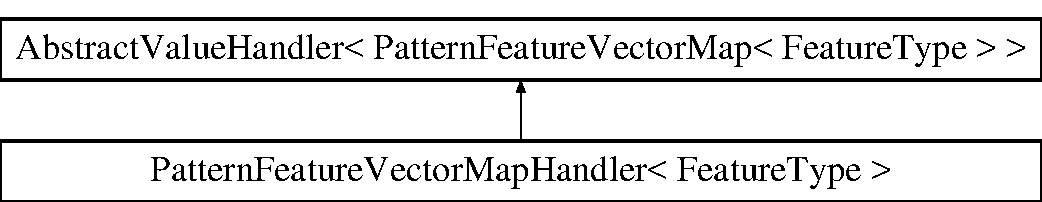
\includegraphics[height=2.000000cm]{classPatternFeatureVectorMapHandler}
\end{center}
\end{figure}
\subsection*{Public Member Functions}
\begin{DoxyCompactItemize}
\item 
virtual std\+::string \hyperlink{classPatternFeatureVectorMapHandler_ac3a86c293fbc3417ae6d8dc13389be82}{id} ()
\item 
void \hyperlink{classPatternFeatureVectorMapHandler_a3956b0d0deccf1a3f36135d084a30627}{read} (std\+::istream $\ast$in, \hyperlink{classPatternFeatureVectorMap}{Pattern\+Feature\+Vector\+Map}$<$ Feature\+Type $>$ \&v)
\item 
void \hyperlink{classPatternFeatureVectorMapHandler_a188df59b0fe05271e3ee90ba20204ffa}{write} (std\+::ostream $\ast$out, \hyperlink{classPatternFeatureVectorMap}{Pattern\+Feature\+Vector\+Map}$<$ Feature\+Type $>$ \&value)
\item 
virtual std\+::string \hyperlink{classPatternFeatureVectorMapHandler_a27faed3107244e4ab0f53e3acea201de}{tostring} (\hyperlink{classPatternFeatureVectorMap}{Pattern\+Feature\+Vector\+Map}$<$ Feature\+Type $>$ \&value)
\item 
unsigned int \hyperlink{classPatternFeatureVectorMapHandler_a67a49821f7c2b8b4d6e1e5be81c36bd4}{count} (\hyperlink{classPatternFeatureVectorMap}{Pattern\+Feature\+Vector\+Map}$<$ Feature\+Type $>$ \&value) const 
\item 
void \hyperlink{classPatternFeatureVectorMapHandler_ab234259fb46c86986d41b0ef81a3b0c0}{add} (\hyperlink{classPatternFeatureVectorMap}{Pattern\+Feature\+Vector\+Map}$<$ Feature\+Type $>$ $\ast$value, const \hyperlink{classIndexReference}{Index\+Reference} \&ref) const 
\item 
void \hyperlink{classPatternFeatureVectorMapHandler_ad69265b8885d3fba7e557a39c3632768}{convertto} (\hyperlink{classPatternFeatureVectorMap}{Pattern\+Feature\+Vector\+Map}$<$ Feature\+Type $>$ $\ast$source, \hyperlink{classPatternFeatureVectorMap}{Pattern\+Feature\+Vector\+Map}$<$ Feature\+Type $>$ $\ast$\&target) const 
\item 
void \hyperlink{classPatternFeatureVectorMapHandler_a8fda95432700c51dd0b7584fb9b47da9}{convertto} (\hyperlink{classPatternFeatureVectorMap}{Pattern\+Feature\+Vector\+Map}$<$ Feature\+Type $>$ $\ast$source, \hyperlink{classIndexedData}{Indexed\+Data} $\ast$\&target) const 
\item 
void \hyperlink{classPatternFeatureVectorMapHandler_a2f61dcfc0704d06b3a0b4ee421bb9a4a}{convertto} (\hyperlink{classPatternFeatureVectorMap}{Pattern\+Feature\+Vector\+Map}$<$ Feature\+Type $>$ $\ast$value, unsigned int $\ast$\&convertedvalue) const 
\end{DoxyCompactItemize}


\subsection{Member Function Documentation}
\hypertarget{classPatternFeatureVectorMapHandler_ab234259fb46c86986d41b0ef81a3b0c0}{}\index{Pattern\+Feature\+Vector\+Map\+Handler@{Pattern\+Feature\+Vector\+Map\+Handler}!add@{add}}
\index{add@{add}!Pattern\+Feature\+Vector\+Map\+Handler@{Pattern\+Feature\+Vector\+Map\+Handler}}
\subsubsection[{add(\+Pattern\+Feature\+Vector\+Map$<$ Feature\+Type $>$ $\ast$value, const Index\+Reference \&ref) const }]{\setlength{\rightskip}{0pt plus 5cm}template$<$class Feature\+Type $>$ void {\bf Pattern\+Feature\+Vector\+Map\+Handler}$<$ Feature\+Type $>$\+::add (
\begin{DoxyParamCaption}
\item[{{\bf Pattern\+Feature\+Vector\+Map}$<$ Feature\+Type $>$ $\ast$}]{value, }
\item[{const {\bf Index\+Reference} \&}]{ref}
\end{DoxyParamCaption}
) const\hspace{0.3cm}{\ttfamily [inline]}, {\ttfamily [virtual]}}\label{classPatternFeatureVectorMapHandler_ab234259fb46c86986d41b0ef81a3b0c0}


Implements \hyperlink{classAbstractValueHandler_a72ecec2580cb5a9a3ba1495a98d08d98}{Abstract\+Value\+Handler$<$ Pattern\+Feature\+Vector\+Map$<$ Feature\+Type $>$ $>$}.

\hypertarget{classPatternFeatureVectorMapHandler_ad69265b8885d3fba7e557a39c3632768}{}\index{Pattern\+Feature\+Vector\+Map\+Handler@{Pattern\+Feature\+Vector\+Map\+Handler}!convertto@{convertto}}
\index{convertto@{convertto}!Pattern\+Feature\+Vector\+Map\+Handler@{Pattern\+Feature\+Vector\+Map\+Handler}}
\subsubsection[{convertto(\+Pattern\+Feature\+Vector\+Map$<$ Feature\+Type $>$ $\ast$source, Pattern\+Feature\+Vector\+Map$<$ Feature\+Type $>$ $\ast$\&target) const }]{\setlength{\rightskip}{0pt plus 5cm}template$<$class Feature\+Type $>$ void {\bf Pattern\+Feature\+Vector\+Map\+Handler}$<$ Feature\+Type $>$\+::convertto (
\begin{DoxyParamCaption}
\item[{{\bf Pattern\+Feature\+Vector\+Map}$<$ Feature\+Type $>$ $\ast$}]{source, }
\item[{{\bf Pattern\+Feature\+Vector\+Map}$<$ Feature\+Type $>$ $\ast$\&}]{target}
\end{DoxyParamCaption}
) const\hspace{0.3cm}{\ttfamily [inline]}, {\ttfamily [virtual]}}\label{classPatternFeatureVectorMapHandler_ad69265b8885d3fba7e557a39c3632768}


Reimplemented from \hyperlink{classAbstractValueHandler_ae89579ec77805153a0acc617202f89b4}{Abstract\+Value\+Handler$<$ Pattern\+Feature\+Vector\+Map$<$ Feature\+Type $>$ $>$}.

\hypertarget{classPatternFeatureVectorMapHandler_a8fda95432700c51dd0b7584fb9b47da9}{}\index{Pattern\+Feature\+Vector\+Map\+Handler@{Pattern\+Feature\+Vector\+Map\+Handler}!convertto@{convertto}}
\index{convertto@{convertto}!Pattern\+Feature\+Vector\+Map\+Handler@{Pattern\+Feature\+Vector\+Map\+Handler}}
\subsubsection[{convertto(\+Pattern\+Feature\+Vector\+Map$<$ Feature\+Type $>$ $\ast$source, Indexed\+Data $\ast$\&target) const }]{\setlength{\rightskip}{0pt plus 5cm}template$<$class Feature\+Type $>$ void {\bf Pattern\+Feature\+Vector\+Map\+Handler}$<$ Feature\+Type $>$\+::convertto (
\begin{DoxyParamCaption}
\item[{{\bf Pattern\+Feature\+Vector\+Map}$<$ Feature\+Type $>$ $\ast$}]{source, }
\item[{{\bf Indexed\+Data} $\ast$\&}]{target}
\end{DoxyParamCaption}
) const\hspace{0.3cm}{\ttfamily [inline]}}\label{classPatternFeatureVectorMapHandler_a8fda95432700c51dd0b7584fb9b47da9}
\hypertarget{classPatternFeatureVectorMapHandler_a2f61dcfc0704d06b3a0b4ee421bb9a4a}{}\index{Pattern\+Feature\+Vector\+Map\+Handler@{Pattern\+Feature\+Vector\+Map\+Handler}!convertto@{convertto}}
\index{convertto@{convertto}!Pattern\+Feature\+Vector\+Map\+Handler@{Pattern\+Feature\+Vector\+Map\+Handler}}
\subsubsection[{convertto(\+Pattern\+Feature\+Vector\+Map$<$ Feature\+Type $>$ $\ast$value, unsigned int $\ast$\&convertedvalue) const }]{\setlength{\rightskip}{0pt plus 5cm}template$<$class Feature\+Type $>$ void {\bf Pattern\+Feature\+Vector\+Map\+Handler}$<$ Feature\+Type $>$\+::convertto (
\begin{DoxyParamCaption}
\item[{{\bf Pattern\+Feature\+Vector\+Map}$<$ Feature\+Type $>$ $\ast$}]{value, }
\item[{unsigned int $\ast$\&}]{convertedvalue}
\end{DoxyParamCaption}
) const\hspace{0.3cm}{\ttfamily [inline]}}\label{classPatternFeatureVectorMapHandler_a2f61dcfc0704d06b3a0b4ee421bb9a4a}
\hypertarget{classPatternFeatureVectorMapHandler_a67a49821f7c2b8b4d6e1e5be81c36bd4}{}\index{Pattern\+Feature\+Vector\+Map\+Handler@{Pattern\+Feature\+Vector\+Map\+Handler}!count@{count}}
\index{count@{count}!Pattern\+Feature\+Vector\+Map\+Handler@{Pattern\+Feature\+Vector\+Map\+Handler}}
\subsubsection[{count(\+Pattern\+Feature\+Vector\+Map$<$ Feature\+Type $>$ \&value) const }]{\setlength{\rightskip}{0pt plus 5cm}template$<$class Feature\+Type $>$ unsigned int {\bf Pattern\+Feature\+Vector\+Map\+Handler}$<$ Feature\+Type $>$\+::count (
\begin{DoxyParamCaption}
\item[{{\bf Pattern\+Feature\+Vector\+Map}$<$ Feature\+Type $>$ \&}]{value}
\end{DoxyParamCaption}
) const\hspace{0.3cm}{\ttfamily [inline]}, {\ttfamily [virtual]}}\label{classPatternFeatureVectorMapHandler_a67a49821f7c2b8b4d6e1e5be81c36bd4}


Implements \hyperlink{classAbstractValueHandler_a1d5941f6ff2afaee0c0bfc89ccb5188e}{Abstract\+Value\+Handler$<$ Pattern\+Feature\+Vector\+Map$<$ Feature\+Type $>$ $>$}.

\hypertarget{classPatternFeatureVectorMapHandler_ac3a86c293fbc3417ae6d8dc13389be82}{}\index{Pattern\+Feature\+Vector\+Map\+Handler@{Pattern\+Feature\+Vector\+Map\+Handler}!id@{id}}
\index{id@{id}!Pattern\+Feature\+Vector\+Map\+Handler@{Pattern\+Feature\+Vector\+Map\+Handler}}
\subsubsection[{id()}]{\setlength{\rightskip}{0pt plus 5cm}template$<$class Feature\+Type $>$ virtual std\+::string {\bf Pattern\+Feature\+Vector\+Map\+Handler}$<$ Feature\+Type $>$\+::id (
\begin{DoxyParamCaption}
{}
\end{DoxyParamCaption}
)\hspace{0.3cm}{\ttfamily [inline]}, {\ttfamily [virtual]}}\label{classPatternFeatureVectorMapHandler_ac3a86c293fbc3417ae6d8dc13389be82}


Reimplemented from \hyperlink{classAbstractValueHandler_a6e2f7abe130cdec1062e51d56e4f9fac}{Abstract\+Value\+Handler$<$ Pattern\+Feature\+Vector\+Map$<$ Feature\+Type $>$ $>$}.

\hypertarget{classPatternFeatureVectorMapHandler_a3956b0d0deccf1a3f36135d084a30627}{}\index{Pattern\+Feature\+Vector\+Map\+Handler@{Pattern\+Feature\+Vector\+Map\+Handler}!read@{read}}
\index{read@{read}!Pattern\+Feature\+Vector\+Map\+Handler@{Pattern\+Feature\+Vector\+Map\+Handler}}
\subsubsection[{read(std\+::istream $\ast$in, Pattern\+Feature\+Vector\+Map$<$ Feature\+Type $>$ \&v)}]{\setlength{\rightskip}{0pt plus 5cm}template$<$class Feature\+Type $>$ void {\bf Pattern\+Feature\+Vector\+Map\+Handler}$<$ Feature\+Type $>$\+::read (
\begin{DoxyParamCaption}
\item[{std\+::istream $\ast$}]{in, }
\item[{{\bf Pattern\+Feature\+Vector\+Map}$<$ Feature\+Type $>$ \&}]{v}
\end{DoxyParamCaption}
)\hspace{0.3cm}{\ttfamily [inline]}, {\ttfamily [virtual]}}\label{classPatternFeatureVectorMapHandler_a3956b0d0deccf1a3f36135d084a30627}


Implements \hyperlink{classAbstractValueHandler_ac7921fae157361b054e467bf96785654}{Abstract\+Value\+Handler$<$ Pattern\+Feature\+Vector\+Map$<$ Feature\+Type $>$ $>$}.

\hypertarget{classPatternFeatureVectorMapHandler_a27faed3107244e4ab0f53e3acea201de}{}\index{Pattern\+Feature\+Vector\+Map\+Handler@{Pattern\+Feature\+Vector\+Map\+Handler}!tostring@{tostring}}
\index{tostring@{tostring}!Pattern\+Feature\+Vector\+Map\+Handler@{Pattern\+Feature\+Vector\+Map\+Handler}}
\subsubsection[{tostring(\+Pattern\+Feature\+Vector\+Map$<$ Feature\+Type $>$ \&value)}]{\setlength{\rightskip}{0pt plus 5cm}template$<$class Feature\+Type $>$ virtual std\+::string {\bf Pattern\+Feature\+Vector\+Map\+Handler}$<$ Feature\+Type $>$\+::tostring (
\begin{DoxyParamCaption}
\item[{{\bf Pattern\+Feature\+Vector\+Map}$<$ Feature\+Type $>$ \&}]{value}
\end{DoxyParamCaption}
)\hspace{0.3cm}{\ttfamily [inline]}, {\ttfamily [virtual]}}\label{classPatternFeatureVectorMapHandler_a27faed3107244e4ab0f53e3acea201de}


Implements \hyperlink{classAbstractValueHandler_a8e56e3bbccc464a47a666352249e6a1b}{Abstract\+Value\+Handler$<$ Pattern\+Feature\+Vector\+Map$<$ Feature\+Type $>$ $>$}.

\hypertarget{classPatternFeatureVectorMapHandler_a188df59b0fe05271e3ee90ba20204ffa}{}\index{Pattern\+Feature\+Vector\+Map\+Handler@{Pattern\+Feature\+Vector\+Map\+Handler}!write@{write}}
\index{write@{write}!Pattern\+Feature\+Vector\+Map\+Handler@{Pattern\+Feature\+Vector\+Map\+Handler}}
\subsubsection[{write(std\+::ostream $\ast$out, Pattern\+Feature\+Vector\+Map$<$ Feature\+Type $>$ \&value)}]{\setlength{\rightskip}{0pt plus 5cm}template$<$class Feature\+Type $>$ void {\bf Pattern\+Feature\+Vector\+Map\+Handler}$<$ Feature\+Type $>$\+::write (
\begin{DoxyParamCaption}
\item[{std\+::ostream $\ast$}]{out, }
\item[{{\bf Pattern\+Feature\+Vector\+Map}$<$ Feature\+Type $>$ \&}]{value}
\end{DoxyParamCaption}
)\hspace{0.3cm}{\ttfamily [inline]}, {\ttfamily [virtual]}}\label{classPatternFeatureVectorMapHandler_a188df59b0fe05271e3ee90ba20204ffa}


Implements \hyperlink{classAbstractValueHandler_aecd2820bc132f8065babbec5cd7458b8}{Abstract\+Value\+Handler$<$ Pattern\+Feature\+Vector\+Map$<$ Feature\+Type $>$ $>$}.



The documentation for this class was generated from the following file\+:\begin{DoxyCompactItemize}
\item 
include/\hyperlink{datatypes_8h}{datatypes.\+h}\end{DoxyCompactItemize}

\hypertarget{classPatternMap}{}\section{Pattern\+Map$<$ Value\+Type, Value\+Handler, Read\+Write\+Size\+Type $>$ Class Template Reference}
\label{classPatternMap}\index{Pattern\+Map$<$ Value\+Type, Value\+Handler, Read\+Write\+Size\+Type $>$@{Pattern\+Map$<$ Value\+Type, Value\+Handler, Read\+Write\+Size\+Type $>$}}


A pattern map storing patterns and their values in a hash map (unordered\+\_\+map).  




{\ttfamily \#include $<$patternstore.\+h$>$}

Inheritance diagram for Pattern\+Map$<$ Value\+Type, Value\+Handler, Read\+Write\+Size\+Type $>$\+:\begin{figure}[H]
\begin{center}
\leavevmode
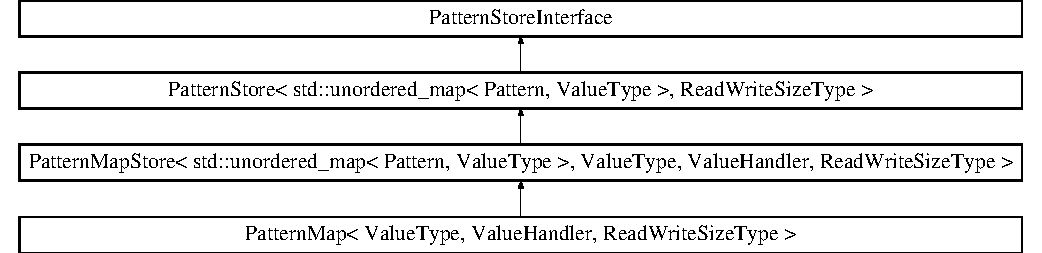
\includegraphics[height=3.393939cm]{classPatternMap}
\end{center}
\end{figure}
\subsection*{Public Types}
\begin{DoxyCompactItemize}
\item 
typedef std\+::unordered\+\_\+map$<$ \hyperlink{classPattern}{Pattern}, Value\+Type $>$\+::\hyperlink{classPatternMap_a4de5ceaff3526d091098b4d82dde2b27}{iterator} \hyperlink{classPatternMap_a4de5ceaff3526d091098b4d82dde2b27}{iterator}
\item 
typedef std\+::unordered\+\_\+map$<$ \hyperlink{classPattern}{Pattern}, Value\+Type $>$\+::\hyperlink{classPatternMap_aba8ff62eadadedc25bf4ea799a322cf3}{const\+\_\+iterator} \hyperlink{classPatternMap_aba8ff62eadadedc25bf4ea799a322cf3}{const\+\_\+iterator}
\end{DoxyCompactItemize}
\subsection*{Public Member Functions}
\begin{DoxyCompactItemize}
\item 
\hyperlink{classPatternMap_af59f2ae4994cc927580751644b00bef0}{Pattern\+Map} ()
\item 
void \hyperlink{classPatternMap_a67628e669cf2995a44769cda83bf8e85}{insert} (const \hyperlink{classPattern}{Pattern} \&pattern, Value\+Type \&value)
\item 
void \hyperlink{classPatternMap_a911511a1b32cef2ee3efb234f66974ce}{insert} (const \hyperlink{classPattern}{Pattern} \&pattern)
\item 
bool \hyperlink{classPatternMap_a038d49e8aed58a207c3e106b086cdab0}{has} (const \hyperlink{classPattern}{Pattern} \&pattern) const 
\item 
bool \hyperlink{classPatternMap_a18587e4b3c6143749b4b96e8f4808cdb}{has} (const \hyperlink{classPatternPointer}{Pattern\+Pointer} \&pattern) const 
\item 
size\+\_\+t \hyperlink{classPatternMap_aed30070f31256d0c1335fa9bd3b5db1c}{size} () const 
\item 
Value\+Type \& \hyperlink{classPatternMap_af08cad16a81aede5cf12f9601b75d697}{operator\mbox{[}$\,$\mbox{]}} (const \hyperlink{classPattern}{Pattern} \&pattern)
\item 
Value\+Type \& \hyperlink{classPatternMap_a790d9a4673f3971c644b120660bfab22}{operator\mbox{[}$\,$\mbox{]}} (const \hyperlink{classPatternPointer}{Pattern\+Pointer} \&pattern)
\item 
\hyperlink{classPatternMap_a4de5ceaff3526d091098b4d82dde2b27}{iterator} \hyperlink{classPatternMap_a6e536f5947c4e1752f91166922c4ae16}{begin} ()
\item 
\hyperlink{classPatternMap_aba8ff62eadadedc25bf4ea799a322cf3}{const\+\_\+iterator} \hyperlink{classPatternMap_addb90b8e3f3721f061757bb5cec64bf2}{begin} () const 
\item 
\hyperlink{classPatternMap_a4de5ceaff3526d091098b4d82dde2b27}{iterator} \hyperlink{classPatternMap_aa5a92eab727e74e54b93f7f7916e26cb}{end} ()
\item 
\hyperlink{classPatternMap_aba8ff62eadadedc25bf4ea799a322cf3}{const\+\_\+iterator} \hyperlink{classPatternMap_a75f67f68fb66a7d15d7f8c75cb08dc8d}{end} () const 
\item 
\hyperlink{classPatternMap_a4de5ceaff3526d091098b4d82dde2b27}{iterator} \hyperlink{classPatternMap_a4f36d73514e80d18f93395a72f81e6bc}{find} (const \hyperlink{classPattern}{Pattern} \&pattern)
\item 
\hyperlink{classPatternMap_aba8ff62eadadedc25bf4ea799a322cf3}{const\+\_\+iterator} \hyperlink{classPatternMap_a685d9bac878f2d8862c6c193ba9de45e}{find} (const \hyperlink{classPattern}{Pattern} \&pattern) const 
\item 
bool \hyperlink{classPatternMap_a96e5a77a5c782f340fe38f5c05ae30c4}{erase} (const \hyperlink{classPattern}{Pattern} \&pattern)
\item 
\hyperlink{classPatternMap_a4de5ceaff3526d091098b4d82dde2b27}{iterator} \hyperlink{classPatternMap_ac7bfe17942e5fb3c1bad7f975b61b650}{erase} (\hyperlink{classPatternMap_aba8ff62eadadedc25bf4ea799a322cf3}{const\+\_\+iterator} position)
\end{DoxyCompactItemize}
\subsection*{Protected Attributes}
\begin{DoxyCompactItemize}
\item 
std\+::unordered\+\_\+map$<$ \hyperlink{classPattern}{Pattern}, Value\+Type $>$ \hyperlink{classPatternMap_af7de0fc22bf41d3d2a7a04260b431cb7}{data}
\end{DoxyCompactItemize}


\subsection{Detailed Description}
\subsubsection*{template$<$class Value\+Type, class Value\+Handler = Base\+Value\+Handler$<$\+Value\+Type$>$, class Read\+Write\+Size\+Type = uint64\+\_\+t$>$class Pattern\+Map$<$ Value\+Type, Value\+Handler, Read\+Write\+Size\+Type $>$}

A pattern map storing patterns and their values in a hash map (unordered\+\_\+map). 


\begin{DoxyTemplParams}{Template Parameters}
{\em Value\+Type} & The type of Value this container stores \\
\hline
{\em Value\+Handler} & A handler class for this type of value \\
\hline
{\em Read\+Write\+Size\+Type} & The data type for addressing, determines the maximum amount of patterns that can be held, only used in serialisation/deserialisation \\
\hline
\end{DoxyTemplParams}


\subsection{Member Typedef Documentation}
\hypertarget{classPatternMap_aba8ff62eadadedc25bf4ea799a322cf3}{}\index{Pattern\+Map@{Pattern\+Map}!const\+\_\+iterator@{const\+\_\+iterator}}
\index{const\+\_\+iterator@{const\+\_\+iterator}!Pattern\+Map@{Pattern\+Map}}
\subsubsection[{const\+\_\+iterator}]{\setlength{\rightskip}{0pt plus 5cm}template$<$class Value\+Type, class Value\+Handler = Base\+Value\+Handler$<$\+Value\+Type$>$, class Read\+Write\+Size\+Type = uint64\+\_\+t$>$ typedef std\+::unordered\+\_\+map$<${\bf Pattern},Value\+Type$>$\+::{\bf const\+\_\+iterator} {\bf Pattern\+Map}$<$ Value\+Type, Value\+Handler, Read\+Write\+Size\+Type $>$\+::{\bf const\+\_\+iterator}}\label{classPatternMap_aba8ff62eadadedc25bf4ea799a322cf3}
\hypertarget{classPatternMap_a4de5ceaff3526d091098b4d82dde2b27}{}\index{Pattern\+Map@{Pattern\+Map}!iterator@{iterator}}
\index{iterator@{iterator}!Pattern\+Map@{Pattern\+Map}}
\subsubsection[{iterator}]{\setlength{\rightskip}{0pt plus 5cm}template$<$class Value\+Type, class Value\+Handler = Base\+Value\+Handler$<$\+Value\+Type$>$, class Read\+Write\+Size\+Type = uint64\+\_\+t$>$ typedef std\+::unordered\+\_\+map$<${\bf Pattern},Value\+Type$>$\+::{\bf iterator} {\bf Pattern\+Map}$<$ Value\+Type, Value\+Handler, Read\+Write\+Size\+Type $>$\+::{\bf iterator}}\label{classPatternMap_a4de5ceaff3526d091098b4d82dde2b27}


\subsection{Constructor \& Destructor Documentation}
\hypertarget{classPatternMap_af59f2ae4994cc927580751644b00bef0}{}\index{Pattern\+Map@{Pattern\+Map}!Pattern\+Map@{Pattern\+Map}}
\index{Pattern\+Map@{Pattern\+Map}!Pattern\+Map@{Pattern\+Map}}
\subsubsection[{Pattern\+Map()}]{\setlength{\rightskip}{0pt plus 5cm}template$<$class Value\+Type, class Value\+Handler = Base\+Value\+Handler$<$\+Value\+Type$>$, class Read\+Write\+Size\+Type = uint64\+\_\+t$>$ {\bf Pattern\+Map}$<$ Value\+Type, Value\+Handler, Read\+Write\+Size\+Type $>$\+::{\bf Pattern\+Map} (
\begin{DoxyParamCaption}
{}
\end{DoxyParamCaption}
)\hspace{0.3cm}{\ttfamily [inline]}}\label{classPatternMap_af59f2ae4994cc927580751644b00bef0}


\subsection{Member Function Documentation}
\hypertarget{classPatternMap_a6e536f5947c4e1752f91166922c4ae16}{}\index{Pattern\+Map@{Pattern\+Map}!begin@{begin}}
\index{begin@{begin}!Pattern\+Map@{Pattern\+Map}}
\subsubsection[{begin()}]{\setlength{\rightskip}{0pt plus 5cm}template$<$class Value\+Type, class Value\+Handler = Base\+Value\+Handler$<$\+Value\+Type$>$, class Read\+Write\+Size\+Type = uint64\+\_\+t$>$ {\bf iterator} {\bf Pattern\+Map}$<$ Value\+Type, Value\+Handler, Read\+Write\+Size\+Type $>$\+::begin (
\begin{DoxyParamCaption}
{}
\end{DoxyParamCaption}
)\hspace{0.3cm}{\ttfamily [inline]}, {\ttfamily [virtual]}}\label{classPatternMap_a6e536f5947c4e1752f91166922c4ae16}


Implements \hyperlink{classPatternMapStore_a2a0a8463a6faa2f2b6636167c06e19af}{Pattern\+Map\+Store$<$ std\+::unordered\+\_\+map$<$ Pattern, Value\+Type $>$, Value\+Type, Value\+Handler, Read\+Write\+Size\+Type $>$}.

\hypertarget{classPatternMap_addb90b8e3f3721f061757bb5cec64bf2}{}\index{Pattern\+Map@{Pattern\+Map}!begin@{begin}}
\index{begin@{begin}!Pattern\+Map@{Pattern\+Map}}
\subsubsection[{begin() const }]{\setlength{\rightskip}{0pt plus 5cm}template$<$class Value\+Type, class Value\+Handler = Base\+Value\+Handler$<$\+Value\+Type$>$, class Read\+Write\+Size\+Type = uint64\+\_\+t$>$ {\bf const\+\_\+iterator} {\bf Pattern\+Map}$<$ Value\+Type, Value\+Handler, Read\+Write\+Size\+Type $>$\+::begin (
\begin{DoxyParamCaption}
{}
\end{DoxyParamCaption}
) const\hspace{0.3cm}{\ttfamily [inline]}}\label{classPatternMap_addb90b8e3f3721f061757bb5cec64bf2}
\hypertarget{classPatternMap_aa5a92eab727e74e54b93f7f7916e26cb}{}\index{Pattern\+Map@{Pattern\+Map}!end@{end}}
\index{end@{end}!Pattern\+Map@{Pattern\+Map}}
\subsubsection[{end()}]{\setlength{\rightskip}{0pt plus 5cm}template$<$class Value\+Type, class Value\+Handler = Base\+Value\+Handler$<$\+Value\+Type$>$, class Read\+Write\+Size\+Type = uint64\+\_\+t$>$ {\bf iterator} {\bf Pattern\+Map}$<$ Value\+Type, Value\+Handler, Read\+Write\+Size\+Type $>$\+::end (
\begin{DoxyParamCaption}
{}
\end{DoxyParamCaption}
)\hspace{0.3cm}{\ttfamily [inline]}, {\ttfamily [virtual]}}\label{classPatternMap_aa5a92eab727e74e54b93f7f7916e26cb}


Implements \hyperlink{classPatternMapStore_a363c63981ea34474b28b2e3a95d376ce}{Pattern\+Map\+Store$<$ std\+::unordered\+\_\+map$<$ Pattern, Value\+Type $>$, Value\+Type, Value\+Handler, Read\+Write\+Size\+Type $>$}.

\hypertarget{classPatternMap_a75f67f68fb66a7d15d7f8c75cb08dc8d}{}\index{Pattern\+Map@{Pattern\+Map}!end@{end}}
\index{end@{end}!Pattern\+Map@{Pattern\+Map}}
\subsubsection[{end() const }]{\setlength{\rightskip}{0pt plus 5cm}template$<$class Value\+Type, class Value\+Handler = Base\+Value\+Handler$<$\+Value\+Type$>$, class Read\+Write\+Size\+Type = uint64\+\_\+t$>$ {\bf const\+\_\+iterator} {\bf Pattern\+Map}$<$ Value\+Type, Value\+Handler, Read\+Write\+Size\+Type $>$\+::end (
\begin{DoxyParamCaption}
{}
\end{DoxyParamCaption}
) const\hspace{0.3cm}{\ttfamily [inline]}}\label{classPatternMap_a75f67f68fb66a7d15d7f8c75cb08dc8d}
\hypertarget{classPatternMap_a96e5a77a5c782f340fe38f5c05ae30c4}{}\index{Pattern\+Map@{Pattern\+Map}!erase@{erase}}
\index{erase@{erase}!Pattern\+Map@{Pattern\+Map}}
\subsubsection[{erase(const Pattern \&pattern)}]{\setlength{\rightskip}{0pt plus 5cm}template$<$class Value\+Type, class Value\+Handler = Base\+Value\+Handler$<$\+Value\+Type$>$, class Read\+Write\+Size\+Type = uint64\+\_\+t$>$ bool {\bf Pattern\+Map}$<$ Value\+Type, Value\+Handler, Read\+Write\+Size\+Type $>$\+::erase (
\begin{DoxyParamCaption}
\item[{const {\bf Pattern} \&}]{pattern}
\end{DoxyParamCaption}
)\hspace{0.3cm}{\ttfamily [inline]}, {\ttfamily [virtual]}}\label{classPatternMap_a96e5a77a5c782f340fe38f5c05ae30c4}


Implements \hyperlink{classPatternMapStore_a60f2926144fbd408b86d9ff5481fd140}{Pattern\+Map\+Store$<$ std\+::unordered\+\_\+map$<$ Pattern, Value\+Type $>$, Value\+Type, Value\+Handler, Read\+Write\+Size\+Type $>$}.

\hypertarget{classPatternMap_ac7bfe17942e5fb3c1bad7f975b61b650}{}\index{Pattern\+Map@{Pattern\+Map}!erase@{erase}}
\index{erase@{erase}!Pattern\+Map@{Pattern\+Map}}
\subsubsection[{erase(const\+\_\+iterator position)}]{\setlength{\rightskip}{0pt plus 5cm}template$<$class Value\+Type, class Value\+Handler = Base\+Value\+Handler$<$\+Value\+Type$>$, class Read\+Write\+Size\+Type = uint64\+\_\+t$>$ {\bf iterator} {\bf Pattern\+Map}$<$ Value\+Type, Value\+Handler, Read\+Write\+Size\+Type $>$\+::erase (
\begin{DoxyParamCaption}
\item[{{\bf const\+\_\+iterator}}]{position}
\end{DoxyParamCaption}
)\hspace{0.3cm}{\ttfamily [inline]}}\label{classPatternMap_ac7bfe17942e5fb3c1bad7f975b61b650}
\hypertarget{classPatternMap_a4f36d73514e80d18f93395a72f81e6bc}{}\index{Pattern\+Map@{Pattern\+Map}!find@{find}}
\index{find@{find}!Pattern\+Map@{Pattern\+Map}}
\subsubsection[{find(const Pattern \&pattern)}]{\setlength{\rightskip}{0pt plus 5cm}template$<$class Value\+Type, class Value\+Handler = Base\+Value\+Handler$<$\+Value\+Type$>$, class Read\+Write\+Size\+Type = uint64\+\_\+t$>$ {\bf iterator} {\bf Pattern\+Map}$<$ Value\+Type, Value\+Handler, Read\+Write\+Size\+Type $>$\+::find (
\begin{DoxyParamCaption}
\item[{const {\bf Pattern} \&}]{pattern}
\end{DoxyParamCaption}
)\hspace{0.3cm}{\ttfamily [inline]}, {\ttfamily [virtual]}}\label{classPatternMap_a4f36d73514e80d18f93395a72f81e6bc}


Implements \hyperlink{classPatternMapStore_ae50e3cdbbf9a503d3381971daec92b54}{Pattern\+Map\+Store$<$ std\+::unordered\+\_\+map$<$ Pattern, Value\+Type $>$, Value\+Type, Value\+Handler, Read\+Write\+Size\+Type $>$}.

\hypertarget{classPatternMap_a685d9bac878f2d8862c6c193ba9de45e}{}\index{Pattern\+Map@{Pattern\+Map}!find@{find}}
\index{find@{find}!Pattern\+Map@{Pattern\+Map}}
\subsubsection[{find(const Pattern \&pattern) const }]{\setlength{\rightskip}{0pt plus 5cm}template$<$class Value\+Type, class Value\+Handler = Base\+Value\+Handler$<$\+Value\+Type$>$, class Read\+Write\+Size\+Type = uint64\+\_\+t$>$ {\bf const\+\_\+iterator} {\bf Pattern\+Map}$<$ Value\+Type, Value\+Handler, Read\+Write\+Size\+Type $>$\+::find (
\begin{DoxyParamCaption}
\item[{const {\bf Pattern} \&}]{pattern}
\end{DoxyParamCaption}
) const\hspace{0.3cm}{\ttfamily [inline]}}\label{classPatternMap_a685d9bac878f2d8862c6c193ba9de45e}
\hypertarget{classPatternMap_a038d49e8aed58a207c3e106b086cdab0}{}\index{Pattern\+Map@{Pattern\+Map}!has@{has}}
\index{has@{has}!Pattern\+Map@{Pattern\+Map}}
\subsubsection[{has(const Pattern \&pattern) const }]{\setlength{\rightskip}{0pt plus 5cm}template$<$class Value\+Type, class Value\+Handler = Base\+Value\+Handler$<$\+Value\+Type$>$, class Read\+Write\+Size\+Type = uint64\+\_\+t$>$ bool {\bf Pattern\+Map}$<$ Value\+Type, Value\+Handler, Read\+Write\+Size\+Type $>$\+::has (
\begin{DoxyParamCaption}
\item[{const {\bf Pattern} \&}]{}
\end{DoxyParamCaption}
) const\hspace{0.3cm}{\ttfamily [inline]}, {\ttfamily [virtual]}}\label{classPatternMap_a038d49e8aed58a207c3e106b086cdab0}
Does the pattern occur in the pattern store? 

Implements \hyperlink{classPatternMapStore_ad9c07c57785e95edbe057e79f94be2c9}{Pattern\+Map\+Store$<$ std\+::unordered\+\_\+map$<$ Pattern, Value\+Type $>$, Value\+Type, Value\+Handler, Read\+Write\+Size\+Type $>$}.

\hypertarget{classPatternMap_a18587e4b3c6143749b4b96e8f4808cdb}{}\index{Pattern\+Map@{Pattern\+Map}!has@{has}}
\index{has@{has}!Pattern\+Map@{Pattern\+Map}}
\subsubsection[{has(const Pattern\+Pointer \&pattern) const }]{\setlength{\rightskip}{0pt plus 5cm}template$<$class Value\+Type, class Value\+Handler = Base\+Value\+Handler$<$\+Value\+Type$>$, class Read\+Write\+Size\+Type = uint64\+\_\+t$>$ bool {\bf Pattern\+Map}$<$ Value\+Type, Value\+Handler, Read\+Write\+Size\+Type $>$\+::has (
\begin{DoxyParamCaption}
\item[{const {\bf Pattern\+Pointer} \&}]{}
\end{DoxyParamCaption}
) const\hspace{0.3cm}{\ttfamily [inline]}, {\ttfamily [virtual]}}\label{classPatternMap_a18587e4b3c6143749b4b96e8f4808cdb}
Does the pattern occur in the pattern store? 

Implements \hyperlink{classPatternMapStore_a00d47f8640efaeb3ce85558b3ee4a6a2}{Pattern\+Map\+Store$<$ std\+::unordered\+\_\+map$<$ Pattern, Value\+Type $>$, Value\+Type, Value\+Handler, Read\+Write\+Size\+Type $>$}.

\hypertarget{classPatternMap_a67628e669cf2995a44769cda83bf8e85}{}\index{Pattern\+Map@{Pattern\+Map}!insert@{insert}}
\index{insert@{insert}!Pattern\+Map@{Pattern\+Map}}
\subsubsection[{insert(const Pattern \&pattern, Value\+Type \&value)}]{\setlength{\rightskip}{0pt plus 5cm}template$<$class Value\+Type, class Value\+Handler = Base\+Value\+Handler$<$\+Value\+Type$>$, class Read\+Write\+Size\+Type = uint64\+\_\+t$>$ void {\bf Pattern\+Map}$<$ Value\+Type, Value\+Handler, Read\+Write\+Size\+Type $>$\+::insert (
\begin{DoxyParamCaption}
\item[{const {\bf Pattern} \&}]{pattern, }
\item[{Value\+Type \&}]{value}
\end{DoxyParamCaption}
)\hspace{0.3cm}{\ttfamily [inline]}, {\ttfamily [virtual]}}\label{classPatternMap_a67628e669cf2995a44769cda83bf8e85}


Implements \hyperlink{classPatternMapStore_a37bcf7aae1c40ccdea57e9a57533a555}{Pattern\+Map\+Store$<$ std\+::unordered\+\_\+map$<$ Pattern, Value\+Type $>$, Value\+Type, Value\+Handler, Read\+Write\+Size\+Type $>$}.

\hypertarget{classPatternMap_a911511a1b32cef2ee3efb234f66974ce}{}\index{Pattern\+Map@{Pattern\+Map}!insert@{insert}}
\index{insert@{insert}!Pattern\+Map@{Pattern\+Map}}
\subsubsection[{insert(const Pattern \&pattern)}]{\setlength{\rightskip}{0pt plus 5cm}template$<$class Value\+Type, class Value\+Handler = Base\+Value\+Handler$<$\+Value\+Type$>$, class Read\+Write\+Size\+Type = uint64\+\_\+t$>$ void {\bf Pattern\+Map}$<$ Value\+Type, Value\+Handler, Read\+Write\+Size\+Type $>$\+::insert (
\begin{DoxyParamCaption}
\item[{const {\bf Pattern} \&}]{pattern}
\end{DoxyParamCaption}
)\hspace{0.3cm}{\ttfamily [inline]}, {\ttfamily [virtual]}}\label{classPatternMap_a911511a1b32cef2ee3efb234f66974ce}


Implements \hyperlink{classPatternStore_a22e091d80efb8182ac49cf6b225f0aa1}{Pattern\+Store$<$ std\+::unordered\+\_\+map$<$ Pattern, Value\+Type $>$, Read\+Write\+Size\+Type $>$}.

\hypertarget{classPatternMap_af08cad16a81aede5cf12f9601b75d697}{}\index{Pattern\+Map@{Pattern\+Map}!operator\mbox{[}$\,$\mbox{]}@{operator[]}}
\index{operator\mbox{[}$\,$\mbox{]}@{operator[]}!Pattern\+Map@{Pattern\+Map}}
\subsubsection[{operator[](const Pattern \&pattern)}]{\setlength{\rightskip}{0pt plus 5cm}template$<$class Value\+Type, class Value\+Handler = Base\+Value\+Handler$<$\+Value\+Type$>$, class Read\+Write\+Size\+Type = uint64\+\_\+t$>$ Value\+Type\& {\bf Pattern\+Map}$<$ Value\+Type, Value\+Handler, Read\+Write\+Size\+Type $>$\+::operator\mbox{[}$\,$\mbox{]} (
\begin{DoxyParamCaption}
\item[{const {\bf Pattern} \&}]{pattern}
\end{DoxyParamCaption}
)\hspace{0.3cm}{\ttfamily [inline]}, {\ttfamily [virtual]}}\label{classPatternMap_af08cad16a81aede5cf12f9601b75d697}


Implements \hyperlink{classPatternMapStore_ac4e8b5a15bb4e3d0f205a979f0d272ab}{Pattern\+Map\+Store$<$ std\+::unordered\+\_\+map$<$ Pattern, Value\+Type $>$, Value\+Type, Value\+Handler, Read\+Write\+Size\+Type $>$}.

\hypertarget{classPatternMap_a790d9a4673f3971c644b120660bfab22}{}\index{Pattern\+Map@{Pattern\+Map}!operator\mbox{[}$\,$\mbox{]}@{operator[]}}
\index{operator\mbox{[}$\,$\mbox{]}@{operator[]}!Pattern\+Map@{Pattern\+Map}}
\subsubsection[{operator[](const Pattern\+Pointer \&pattern)}]{\setlength{\rightskip}{0pt plus 5cm}template$<$class Value\+Type, class Value\+Handler = Base\+Value\+Handler$<$\+Value\+Type$>$, class Read\+Write\+Size\+Type = uint64\+\_\+t$>$ Value\+Type\& {\bf Pattern\+Map}$<$ Value\+Type, Value\+Handler, Read\+Write\+Size\+Type $>$\+::operator\mbox{[}$\,$\mbox{]} (
\begin{DoxyParamCaption}
\item[{const {\bf Pattern\+Pointer} \&}]{pattern}
\end{DoxyParamCaption}
)\hspace{0.3cm}{\ttfamily [inline]}, {\ttfamily [virtual]}}\label{classPatternMap_a790d9a4673f3971c644b120660bfab22}


Implements \hyperlink{classPatternMapStore_ac4f6c5ef2bd7397a33adeb2e72f6d38c}{Pattern\+Map\+Store$<$ std\+::unordered\+\_\+map$<$ Pattern, Value\+Type $>$, Value\+Type, Value\+Handler, Read\+Write\+Size\+Type $>$}.

\hypertarget{classPatternMap_aed30070f31256d0c1335fa9bd3b5db1c}{}\index{Pattern\+Map@{Pattern\+Map}!size@{size}}
\index{size@{size}!Pattern\+Map@{Pattern\+Map}}
\subsubsection[{size() const }]{\setlength{\rightskip}{0pt plus 5cm}template$<$class Value\+Type, class Value\+Handler = Base\+Value\+Handler$<$\+Value\+Type$>$, class Read\+Write\+Size\+Type = uint64\+\_\+t$>$ size\+\_\+t {\bf Pattern\+Map}$<$ Value\+Type, Value\+Handler, Read\+Write\+Size\+Type $>$\+::size (
\begin{DoxyParamCaption}
{}
\end{DoxyParamCaption}
) const\hspace{0.3cm}{\ttfamily [inline]}, {\ttfamily [virtual]}}\label{classPatternMap_aed30070f31256d0c1335fa9bd3b5db1c}
How many patterns are in the pattern store? 

Implements \hyperlink{classPatternMapStore_ab6dc590b4b102f1464301a3fc6c4ec73}{Pattern\+Map\+Store$<$ std\+::unordered\+\_\+map$<$ Pattern, Value\+Type $>$, Value\+Type, Value\+Handler, Read\+Write\+Size\+Type $>$}.



\subsection{Member Data Documentation}
\hypertarget{classPatternMap_af7de0fc22bf41d3d2a7a04260b431cb7}{}\index{Pattern\+Map@{Pattern\+Map}!data@{data}}
\index{data@{data}!Pattern\+Map@{Pattern\+Map}}
\subsubsection[{data}]{\setlength{\rightskip}{0pt plus 5cm}template$<$class Value\+Type, class Value\+Handler = Base\+Value\+Handler$<$\+Value\+Type$>$, class Read\+Write\+Size\+Type = uint64\+\_\+t$>$ std\+::unordered\+\_\+map$<${\bf Pattern}, Value\+Type$>$ {\bf Pattern\+Map}$<$ Value\+Type, Value\+Handler, Read\+Write\+Size\+Type $>$\+::data\hspace{0.3cm}{\ttfamily [protected]}}\label{classPatternMap_af7de0fc22bf41d3d2a7a04260b431cb7}


The documentation for this class was generated from the following file\+:\begin{DoxyCompactItemize}
\item 
include/\hyperlink{patternstore_8h}{patternstore.\+h}\end{DoxyCompactItemize}

\hypertarget{classPatternMapStore}{}\section{Pattern\+Map\+Store$<$ Container\+Type, Value\+Type, Value\+Handler, Read\+Write\+Size\+Type $>$ Class Template Reference}
\label{classPatternMapStore}\index{Pattern\+Map\+Store$<$ Container\+Type, Value\+Type, Value\+Handler, Read\+Write\+Size\+Type $>$@{Pattern\+Map\+Store$<$ Container\+Type, Value\+Type, Value\+Handler, Read\+Write\+Size\+Type $>$}}


Abstract class for map-\/like pattern stores, do not instantiate directly.  




{\ttfamily \#include $<$patternstore.\+h$>$}

Inheritance diagram for Pattern\+Map\+Store$<$ Container\+Type, Value\+Type, Value\+Handler, Read\+Write\+Size\+Type $>$\+:\begin{figure}[H]
\begin{center}
\leavevmode
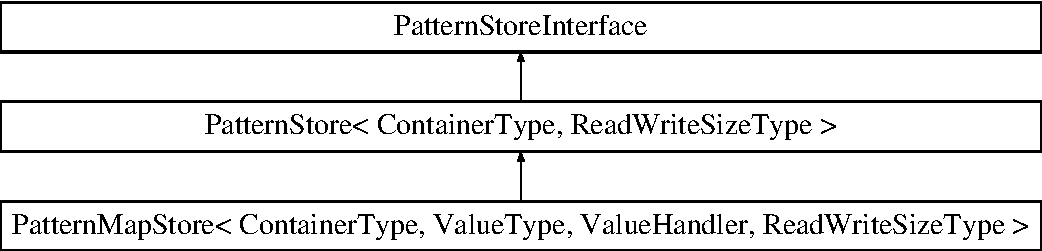
\includegraphics[height=3.000000cm]{classPatternMapStore}
\end{center}
\end{figure}
\subsection*{Public Types}
\begin{DoxyCompactItemize}
\item 
typedef Container\+Type\+::iterator \hyperlink{classPatternMapStore_a918b5de9d2deb6fcc2080a0bb9f53877}{iterator}
\item 
typedef Container\+Type\+::const\+\_\+iterator \hyperlink{classPatternMapStore_a41a18b827340283e8a643a1d526320f4}{const\+\_\+iterator}
\end{DoxyCompactItemize}
\subsection*{Public Member Functions}
\begin{DoxyCompactItemize}
\item 
\hyperlink{classPatternMapStore_af246953d72bedb9ef3741eddb1768ff6}{Pattern\+Map\+Store} ()
\item 
virtual \hyperlink{classPatternMapStore_aa15df2207721ea9d43952add6e5a1ebc}{$\sim$\+Pattern\+Map\+Store} ()
\item 
virtual void \hyperlink{classPatternMapStore_a37bcf7aae1c40ccdea57e9a57533a555}{insert} (const \hyperlink{classPattern}{Pattern} \&pattern, Value\+Type \&value)=0
\item 
virtual bool \hyperlink{classPatternMapStore_ad9c07c57785e95edbe057e79f94be2c9}{has} (const \hyperlink{classPattern}{Pattern} \&) const  =0
\item 
virtual bool \hyperlink{classPatternMapStore_a00d47f8640efaeb3ce85558b3ee4a6a2}{has} (const \hyperlink{classPatternPointer}{Pattern\+Pointer} \&) const  =0
\item 
virtual bool \hyperlink{classPatternMapStore_a60f2926144fbd408b86d9ff5481fd140}{erase} (const \hyperlink{classPattern}{Pattern} \&)=0
\item 
virtual size\+\_\+t \hyperlink{classPatternMapStore_ab6dc590b4b102f1464301a3fc6c4ec73}{size} () const  =0
\item 
virtual Value\+Type \& \hyperlink{classPatternMapStore_ac4e8b5a15bb4e3d0f205a979f0d272ab}{operator\mbox{[}$\,$\mbox{]}} (const \hyperlink{classPattern}{Pattern} \&pattern)=0
\item 
virtual Value\+Type \& \hyperlink{classPatternMapStore_ac4f6c5ef2bd7397a33adeb2e72f6d38c}{operator\mbox{[}$\,$\mbox{]}} (const \hyperlink{classPatternPointer}{Pattern\+Pointer} \&pattern)=0
\item 
virtual Container\+Type\+::iterator \hyperlink{classPatternMapStore_a2a0a8463a6faa2f2b6636167c06e19af}{begin} ()=0
\item 
virtual Container\+Type\+::iterator \hyperlink{classPatternMapStore_a363c63981ea34474b28b2e3a95d376ce}{end} ()=0
\item 
virtual Container\+Type\+::iterator \hyperlink{classPatternMapStore_ae50e3cdbbf9a503d3381971daec92b54}{find} (const \hyperlink{classPattern}{Pattern} \&pattern)=0
\item 
virtual void \hyperlink{classPatternMapStore_aa672214575c57ba24f51996e1eb26902}{write} (std\+::ostream $\ast$out)
\item 
virtual void \hyperlink{classPatternMapStore_abefd53c729c5cdd4916edfc8be1054b2}{write} (std\+::string filename)
\item 
{\footnotesize template$<$class Read\+Value\+Type  = Value\+Type, class Read\+Value\+Handler  = Value\+Handler$>$ }\\void \hyperlink{classPatternMapStore_af6b2ea5515c974d47212bd84b0d39f15}{read} (std\+::istream $\ast$in, int M\+I\+N\+T\+O\+K\+E\+N\+S=0, int M\+I\+N\+L\+E\+N\+G\+T\+H=0, int M\+A\+X\+L\+E\+N\+G\+T\+H=999999, \hyperlink{classPatternStoreInterface}{Pattern\+Store\+Interface} $\ast$constrainstore=N\+U\+L\+L, bool D\+O\+N\+G\+R\+A\+M\+S=true, bool D\+O\+S\+K\+I\+P\+G\+R\+A\+M\+S=true, bool D\+O\+F\+L\+E\+X\+G\+R\+A\+M\+S=true, bool D\+O\+R\+E\+S\+E\+T=false, bool D\+E\+B\+U\+G=false)
\item 
void \hyperlink{classPatternMapStore_af105b594e52f6f730cc5b15d10f145fe}{read} (std\+::string filename, int M\+I\+N\+T\+O\+K\+E\+N\+S=0, int M\+I\+N\+L\+E\+N\+G\+T\+H=0, int M\+A\+X\+L\+E\+N\+G\+T\+H=999999, \hyperlink{classPatternStoreInterface}{Pattern\+Store\+Interface} $\ast$constrainstore=N\+U\+L\+L, bool D\+O\+N\+G\+R\+A\+M\+S=true, bool D\+O\+S\+K\+I\+P\+G\+R\+A\+M\+S=true, bool D\+O\+F\+L\+E\+X\+G\+R\+A\+M\+S=true, bool D\+O\+R\+E\+S\+E\+T=false, bool D\+E\+B\+U\+G=false)
\end{DoxyCompactItemize}
\subsection*{Protected Attributes}
\begin{DoxyCompactItemize}
\item 
Value\+Handler \hyperlink{classPatternMapStore_abdbe9beb478e1719f6edb64272424e5f}{valuehandler}
\end{DoxyCompactItemize}


\subsection{Detailed Description}
\subsubsection*{template$<$class Container\+Type, class Value\+Type, class Value\+Handler, class Read\+Write\+Size\+Type = uint32\+\_\+t$>$class Pattern\+Map\+Store$<$ Container\+Type, Value\+Type, Value\+Handler, Read\+Write\+Size\+Type $>$}

Abstract class for map-\/like pattern stores, do not instantiate directly. 


\begin{DoxyTemplParams}{Template Parameters}
{\em Container\+Type} & The low-\/level container type used (an S\+T\+L container such as set/map). \\
\hline
{\em Value\+Type} & The type of Value this container stores \\
\hline
{\em Value\+Handler} & A handler class for this type of value \\
\hline
{\em Read\+Write\+Size\+Type} & Data type for addressing, influences only the maximum number of items that can be stored (2$\ast$$\ast$64) in the container, as this will be represented in the very beginning of the binary file. No reason to change this unless the container is very deeply nested in others and contains only few items. \\
\hline
\end{DoxyTemplParams}


\subsection{Member Typedef Documentation}
\hypertarget{classPatternMapStore_a41a18b827340283e8a643a1d526320f4}{}\index{Pattern\+Map\+Store@{Pattern\+Map\+Store}!const\+\_\+iterator@{const\+\_\+iterator}}
\index{const\+\_\+iterator@{const\+\_\+iterator}!Pattern\+Map\+Store@{Pattern\+Map\+Store}}
\subsubsection[{const\+\_\+iterator}]{\setlength{\rightskip}{0pt plus 5cm}template$<$class Container\+Type, class Value\+Type, class Value\+Handler, class Read\+Write\+Size\+Type = uint32\+\_\+t$>$ typedef Container\+Type\+::const\+\_\+iterator {\bf Pattern\+Map\+Store}$<$ Container\+Type, Value\+Type, Value\+Handler, Read\+Write\+Size\+Type $>$\+::{\bf const\+\_\+iterator}}\label{classPatternMapStore_a41a18b827340283e8a643a1d526320f4}
\hypertarget{classPatternMapStore_a918b5de9d2deb6fcc2080a0bb9f53877}{}\index{Pattern\+Map\+Store@{Pattern\+Map\+Store}!iterator@{iterator}}
\index{iterator@{iterator}!Pattern\+Map\+Store@{Pattern\+Map\+Store}}
\subsubsection[{iterator}]{\setlength{\rightskip}{0pt plus 5cm}template$<$class Container\+Type, class Value\+Type, class Value\+Handler, class Read\+Write\+Size\+Type = uint32\+\_\+t$>$ typedef Container\+Type\+::iterator {\bf Pattern\+Map\+Store}$<$ Container\+Type, Value\+Type, Value\+Handler, Read\+Write\+Size\+Type $>$\+::{\bf iterator}}\label{classPatternMapStore_a918b5de9d2deb6fcc2080a0bb9f53877}


\subsection{Constructor \& Destructor Documentation}
\hypertarget{classPatternMapStore_af246953d72bedb9ef3741eddb1768ff6}{}\index{Pattern\+Map\+Store@{Pattern\+Map\+Store}!Pattern\+Map\+Store@{Pattern\+Map\+Store}}
\index{Pattern\+Map\+Store@{Pattern\+Map\+Store}!Pattern\+Map\+Store@{Pattern\+Map\+Store}}
\subsubsection[{Pattern\+Map\+Store()}]{\setlength{\rightskip}{0pt plus 5cm}template$<$class Container\+Type, class Value\+Type, class Value\+Handler, class Read\+Write\+Size\+Type = uint32\+\_\+t$>$ {\bf Pattern\+Map\+Store}$<$ Container\+Type, Value\+Type, Value\+Handler, Read\+Write\+Size\+Type $>$\+::{\bf Pattern\+Map\+Store} (
\begin{DoxyParamCaption}
{}
\end{DoxyParamCaption}
)\hspace{0.3cm}{\ttfamily [inline]}}\label{classPatternMapStore_af246953d72bedb9ef3741eddb1768ff6}
\hypertarget{classPatternMapStore_aa15df2207721ea9d43952add6e5a1ebc}{}\index{Pattern\+Map\+Store@{Pattern\+Map\+Store}!````~Pattern\+Map\+Store@{$\sim$\+Pattern\+Map\+Store}}
\index{````~Pattern\+Map\+Store@{$\sim$\+Pattern\+Map\+Store}!Pattern\+Map\+Store@{Pattern\+Map\+Store}}
\subsubsection[{$\sim$\+Pattern\+Map\+Store()}]{\setlength{\rightskip}{0pt plus 5cm}template$<$class Container\+Type, class Value\+Type, class Value\+Handler, class Read\+Write\+Size\+Type = uint32\+\_\+t$>$ virtual {\bf Pattern\+Map\+Store}$<$ Container\+Type, Value\+Type, Value\+Handler, Read\+Write\+Size\+Type $>$\+::$\sim${\bf Pattern\+Map\+Store} (
\begin{DoxyParamCaption}
{}
\end{DoxyParamCaption}
)\hspace{0.3cm}{\ttfamily [inline]}, {\ttfamily [virtual]}}\label{classPatternMapStore_aa15df2207721ea9d43952add6e5a1ebc}


\subsection{Member Function Documentation}
\hypertarget{classPatternMapStore_a2a0a8463a6faa2f2b6636167c06e19af}{}\index{Pattern\+Map\+Store@{Pattern\+Map\+Store}!begin@{begin}}
\index{begin@{begin}!Pattern\+Map\+Store@{Pattern\+Map\+Store}}
\subsubsection[{begin()=0}]{\setlength{\rightskip}{0pt plus 5cm}template$<$class Container\+Type, class Value\+Type, class Value\+Handler, class Read\+Write\+Size\+Type = uint32\+\_\+t$>$ virtual Container\+Type\+::iterator {\bf Pattern\+Map\+Store}$<$ Container\+Type, Value\+Type, Value\+Handler, Read\+Write\+Size\+Type $>$\+::begin (
\begin{DoxyParamCaption}
{}
\end{DoxyParamCaption}
)\hspace{0.3cm}{\ttfamily [pure virtual]}}\label{classPatternMapStore_a2a0a8463a6faa2f2b6636167c06e19af}


Implements \hyperlink{classPatternStore_a9dfc403ac576e1904f4ec326fec1adaa}{Pattern\+Store$<$ Container\+Type, Read\+Write\+Size\+Type $>$}.



Implemented in \hyperlink{classHashOrderedPatternMap_ac103913725b7036ba414453b2204b955}{Hash\+Ordered\+Pattern\+Map$<$ Value\+Type, Value\+Handler, Read\+Write\+Size\+Type $>$}, \hyperlink{classPatternMap_a6e536f5947c4e1752f91166922c4ae16}{Pattern\+Map$<$ Value\+Type, Value\+Handler, Read\+Write\+Size\+Type $>$}, \hyperlink{classPatternMap_a6e536f5947c4e1752f91166922c4ae16}{Pattern\+Map$<$ Pattern\+Map$<$ Value\+Type, Value\+Handler, Nested\+Size\+Type $>$, Pattern\+Store\+Value\+Handler$<$ Pattern\+Map$<$ Value\+Type, Value\+Handler, Nested\+Size\+Type $>$ $>$, uint64\+\_\+t $>$}, \hyperlink{classPatternMap_a6e536f5947c4e1752f91166922c4ae16}{Pattern\+Map$<$ Value\+Type, Value\+Handler, Nested\+Size\+Type $>$}, and \hyperlink{classPatternMap_a6e536f5947c4e1752f91166922c4ae16}{Pattern\+Map$<$ Pattern\+Feature\+Vector\+Map$<$ Feature\+Type $>$, Pattern\+Feature\+Vector\+Map\+Handler$<$ Feature\+Type $>$ $>$}.

\hypertarget{classPatternMapStore_a363c63981ea34474b28b2e3a95d376ce}{}\index{Pattern\+Map\+Store@{Pattern\+Map\+Store}!end@{end}}
\index{end@{end}!Pattern\+Map\+Store@{Pattern\+Map\+Store}}
\subsubsection[{end()=0}]{\setlength{\rightskip}{0pt plus 5cm}template$<$class Container\+Type, class Value\+Type, class Value\+Handler, class Read\+Write\+Size\+Type = uint32\+\_\+t$>$ virtual Container\+Type\+::iterator {\bf Pattern\+Map\+Store}$<$ Container\+Type, Value\+Type, Value\+Handler, Read\+Write\+Size\+Type $>$\+::end (
\begin{DoxyParamCaption}
{}
\end{DoxyParamCaption}
)\hspace{0.3cm}{\ttfamily [pure virtual]}}\label{classPatternMapStore_a363c63981ea34474b28b2e3a95d376ce}


Implements \hyperlink{classPatternStore_aed5adf38c88543123f705e44b4cddfee}{Pattern\+Store$<$ Container\+Type, Read\+Write\+Size\+Type $>$}.



Implemented in \hyperlink{classHashOrderedPatternMap_aa2a8090eed690299d4abeb36ea16fb3d}{Hash\+Ordered\+Pattern\+Map$<$ Value\+Type, Value\+Handler, Read\+Write\+Size\+Type $>$}, \hyperlink{classPatternMap_aa5a92eab727e74e54b93f7f7916e26cb}{Pattern\+Map$<$ Value\+Type, Value\+Handler, Read\+Write\+Size\+Type $>$}, \hyperlink{classPatternMap_aa5a92eab727e74e54b93f7f7916e26cb}{Pattern\+Map$<$ Pattern\+Map$<$ Value\+Type, Value\+Handler, Nested\+Size\+Type $>$, Pattern\+Store\+Value\+Handler$<$ Pattern\+Map$<$ Value\+Type, Value\+Handler, Nested\+Size\+Type $>$ $>$, uint64\+\_\+t $>$}, \hyperlink{classPatternMap_aa5a92eab727e74e54b93f7f7916e26cb}{Pattern\+Map$<$ Value\+Type, Value\+Handler, Nested\+Size\+Type $>$}, and \hyperlink{classPatternMap_aa5a92eab727e74e54b93f7f7916e26cb}{Pattern\+Map$<$ Pattern\+Feature\+Vector\+Map$<$ Feature\+Type $>$, Pattern\+Feature\+Vector\+Map\+Handler$<$ Feature\+Type $>$ $>$}.

\hypertarget{classPatternMapStore_a60f2926144fbd408b86d9ff5481fd140}{}\index{Pattern\+Map\+Store@{Pattern\+Map\+Store}!erase@{erase}}
\index{erase@{erase}!Pattern\+Map\+Store@{Pattern\+Map\+Store}}
\subsubsection[{erase(const Pattern \&)=0}]{\setlength{\rightskip}{0pt plus 5cm}template$<$class Container\+Type, class Value\+Type, class Value\+Handler, class Read\+Write\+Size\+Type = uint32\+\_\+t$>$ virtual bool {\bf Pattern\+Map\+Store}$<$ Container\+Type, Value\+Type, Value\+Handler, Read\+Write\+Size\+Type $>$\+::erase (
\begin{DoxyParamCaption}
\item[{const {\bf Pattern} \&}]{}
\end{DoxyParamCaption}
)\hspace{0.3cm}{\ttfamily [pure virtual]}}\label{classPatternMapStore_a60f2926144fbd408b86d9ff5481fd140}


Implements \hyperlink{classPatternStore_ad8b6d8e1eba917d45e8667ace70f1b1e}{Pattern\+Store$<$ Container\+Type, Read\+Write\+Size\+Type $>$}.



Implemented in \hyperlink{classHashOrderedPatternMap_acc3231c8b727c982ef11c80d3390f8ec}{Hash\+Ordered\+Pattern\+Map$<$ Value\+Type, Value\+Handler, Read\+Write\+Size\+Type $>$}, \hyperlink{classPatternMap_a96e5a77a5c782f340fe38f5c05ae30c4}{Pattern\+Map$<$ Value\+Type, Value\+Handler, Read\+Write\+Size\+Type $>$}, \hyperlink{classPatternMap_a96e5a77a5c782f340fe38f5c05ae30c4}{Pattern\+Map$<$ Pattern\+Map$<$ Value\+Type, Value\+Handler, Nested\+Size\+Type $>$, Pattern\+Store\+Value\+Handler$<$ Pattern\+Map$<$ Value\+Type, Value\+Handler, Nested\+Size\+Type $>$ $>$, uint64\+\_\+t $>$}, \hyperlink{classPatternMap_a96e5a77a5c782f340fe38f5c05ae30c4}{Pattern\+Map$<$ Value\+Type, Value\+Handler, Nested\+Size\+Type $>$}, and \hyperlink{classPatternMap_a96e5a77a5c782f340fe38f5c05ae30c4}{Pattern\+Map$<$ Pattern\+Feature\+Vector\+Map$<$ Feature\+Type $>$, Pattern\+Feature\+Vector\+Map\+Handler$<$ Feature\+Type $>$ $>$}.

\hypertarget{classPatternMapStore_ae50e3cdbbf9a503d3381971daec92b54}{}\index{Pattern\+Map\+Store@{Pattern\+Map\+Store}!find@{find}}
\index{find@{find}!Pattern\+Map\+Store@{Pattern\+Map\+Store}}
\subsubsection[{find(const Pattern \&pattern)=0}]{\setlength{\rightskip}{0pt plus 5cm}template$<$class Container\+Type, class Value\+Type, class Value\+Handler, class Read\+Write\+Size\+Type = uint32\+\_\+t$>$ virtual Container\+Type\+::iterator {\bf Pattern\+Map\+Store}$<$ Container\+Type, Value\+Type, Value\+Handler, Read\+Write\+Size\+Type $>$\+::find (
\begin{DoxyParamCaption}
\item[{const {\bf Pattern} \&}]{pattern}
\end{DoxyParamCaption}
)\hspace{0.3cm}{\ttfamily [pure virtual]}}\label{classPatternMapStore_ae50e3cdbbf9a503d3381971daec92b54}


Implements \hyperlink{classPatternStore_ac8cf692af151c3aad6aea81fa5748957}{Pattern\+Store$<$ Container\+Type, Read\+Write\+Size\+Type $>$}.



Implemented in \hyperlink{classHashOrderedPatternMap_ab0391b67630d9c20ee0069f7197ca9da}{Hash\+Ordered\+Pattern\+Map$<$ Value\+Type, Value\+Handler, Read\+Write\+Size\+Type $>$}, \hyperlink{classPatternMap_a4f36d73514e80d18f93395a72f81e6bc}{Pattern\+Map$<$ Value\+Type, Value\+Handler, Read\+Write\+Size\+Type $>$}, \hyperlink{classPatternMap_a4f36d73514e80d18f93395a72f81e6bc}{Pattern\+Map$<$ Pattern\+Map$<$ Value\+Type, Value\+Handler, Nested\+Size\+Type $>$, Pattern\+Store\+Value\+Handler$<$ Pattern\+Map$<$ Value\+Type, Value\+Handler, Nested\+Size\+Type $>$ $>$, uint64\+\_\+t $>$}, \hyperlink{classPatternMap_a4f36d73514e80d18f93395a72f81e6bc}{Pattern\+Map$<$ Value\+Type, Value\+Handler, Nested\+Size\+Type $>$}, and \hyperlink{classPatternMap_a4f36d73514e80d18f93395a72f81e6bc}{Pattern\+Map$<$ Pattern\+Feature\+Vector\+Map$<$ Feature\+Type $>$, Pattern\+Feature\+Vector\+Map\+Handler$<$ Feature\+Type $>$ $>$}.

\hypertarget{classPatternMapStore_ad9c07c57785e95edbe057e79f94be2c9}{}\index{Pattern\+Map\+Store@{Pattern\+Map\+Store}!has@{has}}
\index{has@{has}!Pattern\+Map\+Store@{Pattern\+Map\+Store}}
\subsubsection[{has(const Pattern \&) const  =0}]{\setlength{\rightskip}{0pt plus 5cm}template$<$class Container\+Type, class Value\+Type, class Value\+Handler, class Read\+Write\+Size\+Type = uint32\+\_\+t$>$ virtual bool {\bf Pattern\+Map\+Store}$<$ Container\+Type, Value\+Type, Value\+Handler, Read\+Write\+Size\+Type $>$\+::has (
\begin{DoxyParamCaption}
\item[{const {\bf Pattern} \&}]{}
\end{DoxyParamCaption}
) const\hspace{0.3cm}{\ttfamily [pure virtual]}}\label{classPatternMapStore_ad9c07c57785e95edbe057e79f94be2c9}
Does the pattern occur in the pattern store? 

Implements \hyperlink{classPatternStore_abdebd74a21912e436531a64fe8b09a6c}{Pattern\+Store$<$ Container\+Type, Read\+Write\+Size\+Type $>$}.



Implemented in \hyperlink{classHashOrderedPatternMap_a8682c2810f85d0c80ed015e388b571ef}{Hash\+Ordered\+Pattern\+Map$<$ Value\+Type, Value\+Handler, Read\+Write\+Size\+Type $>$}, \hyperlink{classPatternMap_a038d49e8aed58a207c3e106b086cdab0}{Pattern\+Map$<$ Value\+Type, Value\+Handler, Read\+Write\+Size\+Type $>$}, \hyperlink{classPatternMap_a038d49e8aed58a207c3e106b086cdab0}{Pattern\+Map$<$ Pattern\+Map$<$ Value\+Type, Value\+Handler, Nested\+Size\+Type $>$, Pattern\+Store\+Value\+Handler$<$ Pattern\+Map$<$ Value\+Type, Value\+Handler, Nested\+Size\+Type $>$ $>$, uint64\+\_\+t $>$}, \hyperlink{classPatternMap_a038d49e8aed58a207c3e106b086cdab0}{Pattern\+Map$<$ Value\+Type, Value\+Handler, Nested\+Size\+Type $>$}, \hyperlink{classPatternMap_a038d49e8aed58a207c3e106b086cdab0}{Pattern\+Map$<$ Pattern\+Feature\+Vector\+Map$<$ Feature\+Type $>$, Pattern\+Feature\+Vector\+Map\+Handler$<$ Feature\+Type $>$ $>$}, and \hyperlink{classPatternAlignmentModel_a4822a730be0dabeebd06771c803b8254}{Pattern\+Alignment\+Model$<$ Feature\+Type $>$}.

\hypertarget{classPatternMapStore_a00d47f8640efaeb3ce85558b3ee4a6a2}{}\index{Pattern\+Map\+Store@{Pattern\+Map\+Store}!has@{has}}
\index{has@{has}!Pattern\+Map\+Store@{Pattern\+Map\+Store}}
\subsubsection[{has(const Pattern\+Pointer \&) const  =0}]{\setlength{\rightskip}{0pt plus 5cm}template$<$class Container\+Type, class Value\+Type, class Value\+Handler, class Read\+Write\+Size\+Type = uint32\+\_\+t$>$ virtual bool {\bf Pattern\+Map\+Store}$<$ Container\+Type, Value\+Type, Value\+Handler, Read\+Write\+Size\+Type $>$\+::has (
\begin{DoxyParamCaption}
\item[{const {\bf Pattern\+Pointer} \&}]{}
\end{DoxyParamCaption}
) const\hspace{0.3cm}{\ttfamily [pure virtual]}}\label{classPatternMapStore_a00d47f8640efaeb3ce85558b3ee4a6a2}
Does the pattern occur in the pattern store? 

Implements \hyperlink{classPatternStore_ad9c8afcf7b7da6acd257c52336751bd2}{Pattern\+Store$<$ Container\+Type, Read\+Write\+Size\+Type $>$}.



Implemented in \hyperlink{classHashOrderedPatternMap_ae2b83d2bcc1378b817044c205bd60651}{Hash\+Ordered\+Pattern\+Map$<$ Value\+Type, Value\+Handler, Read\+Write\+Size\+Type $>$}, \hyperlink{classPatternMap_a18587e4b3c6143749b4b96e8f4808cdb}{Pattern\+Map$<$ Value\+Type, Value\+Handler, Read\+Write\+Size\+Type $>$}, \hyperlink{classPatternMap_a18587e4b3c6143749b4b96e8f4808cdb}{Pattern\+Map$<$ Pattern\+Map$<$ Value\+Type, Value\+Handler, Nested\+Size\+Type $>$, Pattern\+Store\+Value\+Handler$<$ Pattern\+Map$<$ Value\+Type, Value\+Handler, Nested\+Size\+Type $>$ $>$, uint64\+\_\+t $>$}, \hyperlink{classPatternMap_a18587e4b3c6143749b4b96e8f4808cdb}{Pattern\+Map$<$ Value\+Type, Value\+Handler, Nested\+Size\+Type $>$}, \hyperlink{classPatternMap_a18587e4b3c6143749b4b96e8f4808cdb}{Pattern\+Map$<$ Pattern\+Feature\+Vector\+Map$<$ Feature\+Type $>$, Pattern\+Feature\+Vector\+Map\+Handler$<$ Feature\+Type $>$ $>$}, and \hyperlink{classPatternAlignmentModel_ad81e599091c476a9cb121e7e04a4da5a}{Pattern\+Alignment\+Model$<$ Feature\+Type $>$}.

\hypertarget{classPatternMapStore_a37bcf7aae1c40ccdea57e9a57533a555}{}\index{Pattern\+Map\+Store@{Pattern\+Map\+Store}!insert@{insert}}
\index{insert@{insert}!Pattern\+Map\+Store@{Pattern\+Map\+Store}}
\subsubsection[{insert(const Pattern \&pattern, Value\+Type \&value)=0}]{\setlength{\rightskip}{0pt plus 5cm}template$<$class Container\+Type, class Value\+Type, class Value\+Handler, class Read\+Write\+Size\+Type = uint32\+\_\+t$>$ virtual void {\bf Pattern\+Map\+Store}$<$ Container\+Type, Value\+Type, Value\+Handler, Read\+Write\+Size\+Type $>$\+::insert (
\begin{DoxyParamCaption}
\item[{const {\bf Pattern} \&}]{pattern, }
\item[{Value\+Type \&}]{value}
\end{DoxyParamCaption}
)\hspace{0.3cm}{\ttfamily [pure virtual]}}\label{classPatternMapStore_a37bcf7aae1c40ccdea57e9a57533a555}


Implemented in \hyperlink{classHashOrderedPatternMap_aec9cfa54723fbe49e75a4e93109ed0bf}{Hash\+Ordered\+Pattern\+Map$<$ Value\+Type, Value\+Handler, Read\+Write\+Size\+Type $>$}, \hyperlink{classPatternMap_a67628e669cf2995a44769cda83bf8e85}{Pattern\+Map$<$ Value\+Type, Value\+Handler, Read\+Write\+Size\+Type $>$}, \hyperlink{classPatternMap_a67628e669cf2995a44769cda83bf8e85}{Pattern\+Map$<$ Pattern\+Map$<$ Value\+Type, Value\+Handler, Nested\+Size\+Type $>$, Pattern\+Store\+Value\+Handler$<$ Pattern\+Map$<$ Value\+Type, Value\+Handler, Nested\+Size\+Type $>$ $>$, uint64\+\_\+t $>$}, \hyperlink{classPatternMap_a67628e669cf2995a44769cda83bf8e85}{Pattern\+Map$<$ Value\+Type, Value\+Handler, Nested\+Size\+Type $>$}, and \hyperlink{classPatternMap_a67628e669cf2995a44769cda83bf8e85}{Pattern\+Map$<$ Pattern\+Feature\+Vector\+Map$<$ Feature\+Type $>$, Pattern\+Feature\+Vector\+Map\+Handler$<$ Feature\+Type $>$ $>$}.

\hypertarget{classPatternMapStore_ac4e8b5a15bb4e3d0f205a979f0d272ab}{}\index{Pattern\+Map\+Store@{Pattern\+Map\+Store}!operator\mbox{[}$\,$\mbox{]}@{operator[]}}
\index{operator\mbox{[}$\,$\mbox{]}@{operator[]}!Pattern\+Map\+Store@{Pattern\+Map\+Store}}
\subsubsection[{operator[](const Pattern \&pattern)=0}]{\setlength{\rightskip}{0pt plus 5cm}template$<$class Container\+Type, class Value\+Type, class Value\+Handler, class Read\+Write\+Size\+Type = uint32\+\_\+t$>$ virtual Value\+Type\& {\bf Pattern\+Map\+Store}$<$ Container\+Type, Value\+Type, Value\+Handler, Read\+Write\+Size\+Type $>$\+::operator\mbox{[}$\,$\mbox{]} (
\begin{DoxyParamCaption}
\item[{const {\bf Pattern} \&}]{pattern}
\end{DoxyParamCaption}
)\hspace{0.3cm}{\ttfamily [pure virtual]}}\label{classPatternMapStore_ac4e8b5a15bb4e3d0f205a979f0d272ab}


Implemented in \hyperlink{classHashOrderedPatternMap_ac37c92e91eb149eaa271054156264328}{Hash\+Ordered\+Pattern\+Map$<$ Value\+Type, Value\+Handler, Read\+Write\+Size\+Type $>$}, \hyperlink{classPatternMap_af08cad16a81aede5cf12f9601b75d697}{Pattern\+Map$<$ Value\+Type, Value\+Handler, Read\+Write\+Size\+Type $>$}, \hyperlink{classPatternMap_af08cad16a81aede5cf12f9601b75d697}{Pattern\+Map$<$ Pattern\+Map$<$ Value\+Type, Value\+Handler, Nested\+Size\+Type $>$, Pattern\+Store\+Value\+Handler$<$ Pattern\+Map$<$ Value\+Type, Value\+Handler, Nested\+Size\+Type $>$ $>$, uint64\+\_\+t $>$}, \hyperlink{classPatternMap_af08cad16a81aede5cf12f9601b75d697}{Pattern\+Map$<$ Value\+Type, Value\+Handler, Nested\+Size\+Type $>$}, and \hyperlink{classPatternMap_af08cad16a81aede5cf12f9601b75d697}{Pattern\+Map$<$ Pattern\+Feature\+Vector\+Map$<$ Feature\+Type $>$, Pattern\+Feature\+Vector\+Map\+Handler$<$ Feature\+Type $>$ $>$}.

\hypertarget{classPatternMapStore_ac4f6c5ef2bd7397a33adeb2e72f6d38c}{}\index{Pattern\+Map\+Store@{Pattern\+Map\+Store}!operator\mbox{[}$\,$\mbox{]}@{operator[]}}
\index{operator\mbox{[}$\,$\mbox{]}@{operator[]}!Pattern\+Map\+Store@{Pattern\+Map\+Store}}
\subsubsection[{operator[](const Pattern\+Pointer \&pattern)=0}]{\setlength{\rightskip}{0pt plus 5cm}template$<$class Container\+Type, class Value\+Type, class Value\+Handler, class Read\+Write\+Size\+Type = uint32\+\_\+t$>$ virtual Value\+Type\& {\bf Pattern\+Map\+Store}$<$ Container\+Type, Value\+Type, Value\+Handler, Read\+Write\+Size\+Type $>$\+::operator\mbox{[}$\,$\mbox{]} (
\begin{DoxyParamCaption}
\item[{const {\bf Pattern\+Pointer} \&}]{pattern}
\end{DoxyParamCaption}
)\hspace{0.3cm}{\ttfamily [pure virtual]}}\label{classPatternMapStore_ac4f6c5ef2bd7397a33adeb2e72f6d38c}


Implemented in \hyperlink{classHashOrderedPatternMap_a65a2aa5b240f6d88b205273331f212b9}{Hash\+Ordered\+Pattern\+Map$<$ Value\+Type, Value\+Handler, Read\+Write\+Size\+Type $>$}, \hyperlink{classPatternMap_a790d9a4673f3971c644b120660bfab22}{Pattern\+Map$<$ Value\+Type, Value\+Handler, Read\+Write\+Size\+Type $>$}, \hyperlink{classPatternMap_a790d9a4673f3971c644b120660bfab22}{Pattern\+Map$<$ Pattern\+Map$<$ Value\+Type, Value\+Handler, Nested\+Size\+Type $>$, Pattern\+Store\+Value\+Handler$<$ Pattern\+Map$<$ Value\+Type, Value\+Handler, Nested\+Size\+Type $>$ $>$, uint64\+\_\+t $>$}, \hyperlink{classPatternMap_a790d9a4673f3971c644b120660bfab22}{Pattern\+Map$<$ Value\+Type, Value\+Handler, Nested\+Size\+Type $>$}, and \hyperlink{classPatternMap_a790d9a4673f3971c644b120660bfab22}{Pattern\+Map$<$ Pattern\+Feature\+Vector\+Map$<$ Feature\+Type $>$, Pattern\+Feature\+Vector\+Map\+Handler$<$ Feature\+Type $>$ $>$}.

\hypertarget{classPatternMapStore_af6b2ea5515c974d47212bd84b0d39f15}{}\index{Pattern\+Map\+Store@{Pattern\+Map\+Store}!read@{read}}
\index{read@{read}!Pattern\+Map\+Store@{Pattern\+Map\+Store}}
\subsubsection[{read(std\+::istream $\ast$in, int M\+I\+N\+T\+O\+K\+E\+N\+S=0, int M\+I\+N\+L\+E\+N\+G\+T\+H=0, int M\+A\+X\+L\+E\+N\+G\+T\+H=999999, Pattern\+Store\+Interface $\ast$constrainstore=\+N\+U\+L\+L, bool D\+O\+N\+G\+R\+A\+M\+S=true, bool D\+O\+S\+K\+I\+P\+G\+R\+A\+M\+S=true, bool D\+O\+F\+L\+E\+X\+G\+R\+A\+M\+S=true, bool D\+O\+R\+E\+S\+E\+T=false, bool D\+E\+B\+U\+G=false)}]{\setlength{\rightskip}{0pt plus 5cm}template$<$class Container\+Type, class Value\+Type, class Value\+Handler, class Read\+Write\+Size\+Type = uint32\+\_\+t$>$ template$<$class Read\+Value\+Type  = Value\+Type, class Read\+Value\+Handler  = Value\+Handler$>$ void {\bf Pattern\+Map\+Store}$<$ Container\+Type, Value\+Type, Value\+Handler, Read\+Write\+Size\+Type $>$\+::read (
\begin{DoxyParamCaption}
\item[{std\+::istream $\ast$}]{in, }
\item[{int}]{M\+I\+N\+T\+O\+K\+E\+N\+S = {\ttfamily 0}, }
\item[{int}]{M\+I\+N\+L\+E\+N\+G\+T\+H = {\ttfamily 0}, }
\item[{int}]{M\+A\+X\+L\+E\+N\+G\+T\+H = {\ttfamily 999999}, }
\item[{{\bf Pattern\+Store\+Interface} $\ast$}]{constrainstore = {\ttfamily NULL}, }
\item[{bool}]{D\+O\+N\+G\+R\+A\+M\+S = {\ttfamily true}, }
\item[{bool}]{D\+O\+S\+K\+I\+P\+G\+R\+A\+M\+S = {\ttfamily true}, }
\item[{bool}]{D\+O\+F\+L\+E\+X\+G\+R\+A\+M\+S = {\ttfamily true}, }
\item[{bool}]{D\+O\+R\+E\+S\+E\+T = {\ttfamily false}, }
\item[{bool}]{D\+E\+B\+U\+G = {\ttfamily false}}
\end{DoxyParamCaption}
)\hspace{0.3cm}{\ttfamily [inline]}}\label{classPatternMapStore_af6b2ea5515c974d47212bd84b0d39f15}
Read a map from input stream (in binary format) \hypertarget{classPatternMapStore_af105b594e52f6f730cc5b15d10f145fe}{}\index{Pattern\+Map\+Store@{Pattern\+Map\+Store}!read@{read}}
\index{read@{read}!Pattern\+Map\+Store@{Pattern\+Map\+Store}}
\subsubsection[{read(std\+::string filename, int M\+I\+N\+T\+O\+K\+E\+N\+S=0, int M\+I\+N\+L\+E\+N\+G\+T\+H=0, int M\+A\+X\+L\+E\+N\+G\+T\+H=999999, Pattern\+Store\+Interface $\ast$constrainstore=\+N\+U\+L\+L, bool D\+O\+N\+G\+R\+A\+M\+S=true, bool D\+O\+S\+K\+I\+P\+G\+R\+A\+M\+S=true, bool D\+O\+F\+L\+E\+X\+G\+R\+A\+M\+S=true, bool D\+O\+R\+E\+S\+E\+T=false, bool D\+E\+B\+U\+G=false)}]{\setlength{\rightskip}{0pt plus 5cm}template$<$class Container\+Type, class Value\+Type, class Value\+Handler, class Read\+Write\+Size\+Type = uint32\+\_\+t$>$ void {\bf Pattern\+Map\+Store}$<$ Container\+Type, Value\+Type, Value\+Handler, Read\+Write\+Size\+Type $>$\+::read (
\begin{DoxyParamCaption}
\item[{std\+::string}]{filename, }
\item[{int}]{M\+I\+N\+T\+O\+K\+E\+N\+S = {\ttfamily 0}, }
\item[{int}]{M\+I\+N\+L\+E\+N\+G\+T\+H = {\ttfamily 0}, }
\item[{int}]{M\+A\+X\+L\+E\+N\+G\+T\+H = {\ttfamily 999999}, }
\item[{{\bf Pattern\+Store\+Interface} $\ast$}]{constrainstore = {\ttfamily NULL}, }
\item[{bool}]{D\+O\+N\+G\+R\+A\+M\+S = {\ttfamily true}, }
\item[{bool}]{D\+O\+S\+K\+I\+P\+G\+R\+A\+M\+S = {\ttfamily true}, }
\item[{bool}]{D\+O\+F\+L\+E\+X\+G\+R\+A\+M\+S = {\ttfamily true}, }
\item[{bool}]{D\+O\+R\+E\+S\+E\+T = {\ttfamily false}, }
\item[{bool}]{D\+E\+B\+U\+G = {\ttfamily false}}
\end{DoxyParamCaption}
)\hspace{0.3cm}{\ttfamily [inline]}}\label{classPatternMapStore_af105b594e52f6f730cc5b15d10f145fe}
Read a map from file (in binary format) \hypertarget{classPatternMapStore_ab6dc590b4b102f1464301a3fc6c4ec73}{}\index{Pattern\+Map\+Store@{Pattern\+Map\+Store}!size@{size}}
\index{size@{size}!Pattern\+Map\+Store@{Pattern\+Map\+Store}}
\subsubsection[{size() const  =0}]{\setlength{\rightskip}{0pt plus 5cm}template$<$class Container\+Type, class Value\+Type, class Value\+Handler, class Read\+Write\+Size\+Type = uint32\+\_\+t$>$ virtual size\+\_\+t {\bf Pattern\+Map\+Store}$<$ Container\+Type, Value\+Type, Value\+Handler, Read\+Write\+Size\+Type $>$\+::size (
\begin{DoxyParamCaption}
{}
\end{DoxyParamCaption}
) const\hspace{0.3cm}{\ttfamily [pure virtual]}}\label{classPatternMapStore_ab6dc590b4b102f1464301a3fc6c4ec73}
How many patterns are in the pattern store? 

Implements \hyperlink{classPatternStore_a586751d731a509da5865d5863d56a8e4}{Pattern\+Store$<$ Container\+Type, Read\+Write\+Size\+Type $>$}.



Implemented in \hyperlink{classHashOrderedPatternMap_a5a48798964b7d667950f41630d3bf708}{Hash\+Ordered\+Pattern\+Map$<$ Value\+Type, Value\+Handler, Read\+Write\+Size\+Type $>$}, \hyperlink{classPatternMap_aed30070f31256d0c1335fa9bd3b5db1c}{Pattern\+Map$<$ Value\+Type, Value\+Handler, Read\+Write\+Size\+Type $>$}, \hyperlink{classPatternMap_aed30070f31256d0c1335fa9bd3b5db1c}{Pattern\+Map$<$ Pattern\+Map$<$ Value\+Type, Value\+Handler, Nested\+Size\+Type $>$, Pattern\+Store\+Value\+Handler$<$ Pattern\+Map$<$ Value\+Type, Value\+Handler, Nested\+Size\+Type $>$ $>$, uint64\+\_\+t $>$}, \hyperlink{classPatternMap_aed30070f31256d0c1335fa9bd3b5db1c}{Pattern\+Map$<$ Value\+Type, Value\+Handler, Nested\+Size\+Type $>$}, \hyperlink{classPatternMap_aed30070f31256d0c1335fa9bd3b5db1c}{Pattern\+Map$<$ Pattern\+Feature\+Vector\+Map$<$ Feature\+Type $>$, Pattern\+Feature\+Vector\+Map\+Handler$<$ Feature\+Type $>$ $>$}, and \hyperlink{classPatternAlignmentModel_a7e4b2a69fd2e0852af0ed6ffaf6c51dc}{Pattern\+Alignment\+Model$<$ Feature\+Type $>$}.

\hypertarget{classPatternMapStore_aa672214575c57ba24f51996e1eb26902}{}\index{Pattern\+Map\+Store@{Pattern\+Map\+Store}!write@{write}}
\index{write@{write}!Pattern\+Map\+Store@{Pattern\+Map\+Store}}
\subsubsection[{write(std\+::ostream $\ast$out)}]{\setlength{\rightskip}{0pt plus 5cm}template$<$class Container\+Type, class Value\+Type, class Value\+Handler, class Read\+Write\+Size\+Type = uint32\+\_\+t$>$ virtual void {\bf Pattern\+Map\+Store}$<$ Container\+Type, Value\+Type, Value\+Handler, Read\+Write\+Size\+Type $>$\+::write (
\begin{DoxyParamCaption}
\item[{std\+::ostream $\ast$}]{out}
\end{DoxyParamCaption}
)\hspace{0.3cm}{\ttfamily [inline]}, {\ttfamily [virtual]}}\label{classPatternMapStore_aa672214575c57ba24f51996e1eb26902}
Write the map to stream output (in binary format) 

Implements \hyperlink{classPatternStore_ac491b99964c6b4c99f5c40519d0c8ccc}{Pattern\+Store$<$ Container\+Type, Read\+Write\+Size\+Type $>$}.



Reimplemented in \hyperlink{classPatternAlignmentModel_a335c3f85686db801fafeb328bf8df5e8}{Pattern\+Alignment\+Model$<$ Feature\+Type $>$}.

\hypertarget{classPatternMapStore_abefd53c729c5cdd4916edfc8be1054b2}{}\index{Pattern\+Map\+Store@{Pattern\+Map\+Store}!write@{write}}
\index{write@{write}!Pattern\+Map\+Store@{Pattern\+Map\+Store}}
\subsubsection[{write(std\+::string filename)}]{\setlength{\rightskip}{0pt plus 5cm}template$<$class Container\+Type, class Value\+Type, class Value\+Handler, class Read\+Write\+Size\+Type = uint32\+\_\+t$>$ virtual void {\bf Pattern\+Map\+Store}$<$ Container\+Type, Value\+Type, Value\+Handler, Read\+Write\+Size\+Type $>$\+::write (
\begin{DoxyParamCaption}
\item[{std\+::string}]{filename}
\end{DoxyParamCaption}
)\hspace{0.3cm}{\ttfamily [inline]}, {\ttfamily [virtual]}}\label{classPatternMapStore_abefd53c729c5cdd4916edfc8be1054b2}
Write the map to file (in binary format) 

Reimplemented in \hyperlink{classPatternAlignmentModel_a9648856710033da53fa87f7fd52ddab1}{Pattern\+Alignment\+Model$<$ Feature\+Type $>$}.



\subsection{Member Data Documentation}
\hypertarget{classPatternMapStore_abdbe9beb478e1719f6edb64272424e5f}{}\index{Pattern\+Map\+Store@{Pattern\+Map\+Store}!valuehandler@{valuehandler}}
\index{valuehandler@{valuehandler}!Pattern\+Map\+Store@{Pattern\+Map\+Store}}
\subsubsection[{valuehandler}]{\setlength{\rightskip}{0pt plus 5cm}template$<$class Container\+Type, class Value\+Type, class Value\+Handler, class Read\+Write\+Size\+Type = uint32\+\_\+t$>$ Value\+Handler {\bf Pattern\+Map\+Store}$<$ Container\+Type, Value\+Type, Value\+Handler, Read\+Write\+Size\+Type $>$\+::valuehandler\hspace{0.3cm}{\ttfamily [protected]}}\label{classPatternMapStore_abdbe9beb478e1719f6edb64272424e5f}


The documentation for this class was generated from the following file\+:\begin{DoxyCompactItemize}
\item 
include/\hyperlink{patternstore_8h}{patternstore.\+h}\end{DoxyCompactItemize}

\hypertarget{classPatternModel}{}\section{Pattern\+Model$<$ Value\+Type, Value\+Handler, Map\+Type $>$ Class Template Reference}
\label{classPatternModel}\index{Pattern\+Model$<$ Value\+Type, Value\+Handler, Map\+Type $>$@{Pattern\+Model$<$ Value\+Type, Value\+Handler, Map\+Type $>$}}


A model mapping patterns to values, gigh-\/level interface.  




{\ttfamily \#include $<$patternmodel.\+h$>$}

Inheritance diagram for Pattern\+Model$<$ Value\+Type, Value\+Handler, Map\+Type $>$\+:\begin{figure}[H]
\begin{center}
\leavevmode
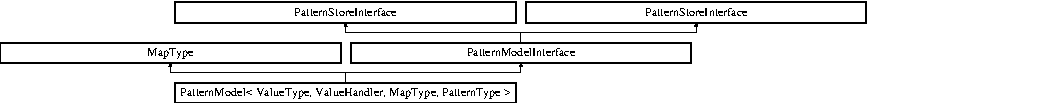
\includegraphics[height=1.702128cm]{classPatternModel}
\end{center}
\end{figure}
\subsection*{Public Types}
\begin{DoxyCompactItemize}
\item 
typedef Map\+Type\+::iterator \hyperlink{classPatternModel_a8aedb15ca2b6f5e3d619c1878d5c0639}{iterator}
\item 
typedef Map\+Type\+::const\+\_\+iterator \hyperlink{classPatternModel_aecfc44c56122e8037bb634a3d66bac0a}{const\+\_\+iterator}
\end{DoxyCompactItemize}
\subsection*{Public Member Functions}
\begin{DoxyCompactItemize}
\item 
\hyperlink{classPatternModel_ade6d8f3c3bae062c06881d96809ea4ff}{Pattern\+Model} (\hyperlink{classIndexedCorpus}{Indexed\+Corpus} $\ast$corpus=N\+U\+L\+L)
\item 
\hyperlink{classPatternModel_a9f1e66e0893ead99e75013cb578cd54a}{Pattern\+Model} (std\+::istream $\ast$f, \hyperlink{classPatternModelOptions}{Pattern\+Model\+Options} options, \hyperlink{classPatternModelInterface}{Pattern\+Model\+Interface} $\ast$constrainmodel=N\+U\+L\+L, \hyperlink{classIndexedCorpus}{Indexed\+Corpus} $\ast$corpus=N\+U\+L\+L)
\item 
\hyperlink{classPatternModel_afd68d5b590a3b477f7fdee2921755a44}{Pattern\+Model} (const std\+::string filename, const \hyperlink{classPatternModelOptions}{Pattern\+Model\+Options} options, \hyperlink{classPatternModelInterface}{Pattern\+Model\+Interface} $\ast$constrainmodel=N\+U\+L\+L, \hyperlink{classIndexedCorpus}{Indexed\+Corpus} $\ast$corpus=N\+U\+L\+L)
\item 
virtual int \hyperlink{classPatternModel_aadea1e70400eb2aeced1ca1648cf9cd9}{getmodeltype} () const 
\item 
virtual int \hyperlink{classPatternModel_ac2f98f98d449951caa82894be78e9fe6}{getmodelversion} () const 
\item 
virtual size\+\_\+t \hyperlink{classPatternModel_a25f387acaf981af9962195bd05b3e7e2}{size} () const 
\item 
virtual bool \hyperlink{classPatternModel_a577eb056f583b4efc943ac4e7a581b1b}{has} (const \hyperlink{classPattern}{Pattern} \&pattern) const 
\item 
virtual bool \hyperlink{classPatternModel_af94a590e3c5eacde04cb55430198acfa}{has} (const \hyperlink{classPatternPointer}{Pattern\+Pointer} \&pattern) const 
\item 
virtual void \hyperlink{classPatternModel_a26de418f6998cac0f484a958597afccc}{load} (std\+::string filename, const \hyperlink{classPatternModelOptions}{Pattern\+Model\+Options} options, \hyperlink{classPatternModelInterface}{Pattern\+Model\+Interface} $\ast$constrainmodel=N\+U\+L\+L)
\item 
virtual void \hyperlink{classPatternModel_acbfb81964c7a6eb13d846dc11d2cc667}{load} (std\+::istream $\ast$f, const \hyperlink{classPatternModelOptions}{Pattern\+Model\+Options} options, \hyperlink{classPatternModelInterface}{Pattern\+Model\+Interface} $\ast$constrainmodel=N\+U\+L\+L)
\item 
\hyperlink{classPatternModelInterface}{Pattern\+Model\+Interface} $\ast$ \hyperlink{classPatternModel_a837bdbf478b7ea8a51ad674418926175}{getinterface} ()
\item 
virtual void \hyperlink{classPatternModel_ac1e8a9a955f8da64abe95179482a6b55}{train} (std\+::istream $\ast$in, \hyperlink{classPatternModelOptions}{Pattern\+Model\+Options} options, \hyperlink{classPatternModelInterface}{Pattern\+Model\+Interface} $\ast$constrainbymodel=N\+U\+L\+L)
\item 
virtual void \hyperlink{classPatternModel_ac2390acee4c9aeecf1bce2d0b312bb4c}{train} (const std\+::string filename, const \hyperlink{classPatternModelOptions}{Pattern\+Model\+Options} options, \hyperlink{classPatternModelInterface}{Pattern\+Model\+Interface} $\ast$constrainbymodel=N\+U\+L\+L)
\item 
virtual int \hyperlink{classPatternModel_aa8a7898c399c670792af12f509adcd28}{computeskipgrams} (const \hyperlink{classPattern}{Pattern} \&pattern, int mintokens=2, const \hyperlink{classIndexReference}{Index\+Reference} $\ast$singleref=N\+U\+L\+L, const \hyperlink{classIndexedData}{Indexed\+Data} $\ast$multiplerefs=N\+U\+L\+L, \hyperlink{classPatternModelInterface}{Pattern\+Model\+Interface} $\ast$constrainbymodel=N\+U\+L\+L, std\+::vector$<$ \hyperlink{classPattern}{Pattern} $>$ $\ast$targetcontainer=N\+U\+L\+L, const bool exhaustive=false, const bool D\+E\+B\+U\+G=false)
\item 
virtual int \hyperlink{classPatternModel_a00b3338b6e79a3dbc9b5f95cb0171494}{computeskipgrams} (const \hyperlink{classPattern}{Pattern} \&pattern, \hyperlink{classPatternModelOptions}{Pattern\+Model\+Options} \&options, const \hyperlink{classIndexReference}{Index\+Reference} $\ast$singleref=N\+U\+L\+L, const \hyperlink{classIndexedData}{Indexed\+Data} $\ast$multiplerefs=N\+U\+L\+L, \hyperlink{classPatternModelInterface}{Pattern\+Model\+Interface} $\ast$constrainbymodel=N\+U\+L\+L, const bool exhaustive=false)
\item 
virtual std\+::vector$<$ \hyperlink{classPattern}{Pattern} $>$ \hyperlink{classPatternModel_aa4aa18a4d9e7554a3c798872e915e8a0}{findskipgrams} (const \hyperlink{classPattern}{Pattern} \&pattern, unsigned int occurrencethreshold=1)
\item 
virtual void \hyperlink{classPatternModel_acd4e0ecc0e796c894b994859b2c5ffb6}{trainskipgrams} (const \hyperlink{classPatternModelOptions}{Pattern\+Model\+Options} options, \hyperlink{classPatternModelInterface}{Pattern\+Model\+Interface} $\ast$constrainbymodel=N\+U\+L\+L)
\item 
void \hyperlink{classPatternModel_a21fb390761ae0fc47e3a48621c94698b}{test} (Map\+Type \&target, std\+::istream $\ast$in)
\item 
void \hyperlink{classPatternModel_a3456e788caacd51fe3c7fb8fdf547723}{write} (std\+::ostream $\ast$out)
\item 
void \hyperlink{classPatternModel_a73654320cd52e691fd7df037cf3ff013}{write} (const std\+::string filename)
\item 
virtual int \hyperlink{classPatternModel_ac0d63c6c6ada696e3a247e25df8487ec}{maxlength} () const 
\item 
virtual int \hyperlink{classPatternModel_a4777ec9b1e76ef3c2ccbc981dad15129}{minlength} () const 
\item 
virtual unsigned int \hyperlink{classPatternModel_a8f5bc659abbbdd456937e85642a97d40}{occurrencecount} (const \hyperlink{classPattern}{Pattern} \&pattern)
\item 
virtual Value\+Type $\ast$ \hyperlink{classPatternModel_aaec0fa3d026d88bc5b8e2dc5f0994015}{getdata} (const \hyperlink{classPattern}{Pattern} \&pattern, bool makeifnew=false)
\item 
virtual Value\+Type $\ast$ \hyperlink{classPatternModel_a1baf331b3a10a45fdadd6a835a744cf3}{getdata} (const \hyperlink{classPatternPointer}{Pattern\+Pointer} \&patternpointer, bool makeifnew=false)
\item 
virtual unsigned int \hyperlink{classPatternModel_af5df3d30417804589c552320add3285a}{types} ()
\item 
virtual unsigned int \hyperlink{classPatternModel_afac99feddfa4cf1dc44090c5148e518a}{tokens} () const 
\item 
unsigned char \hyperlink{classPatternModel_a7df468e440b875af0d9321d090f87dab}{type} () const 
\item 
unsigned char \hyperlink{classPatternModel_af56c31e031bb51d47e98cc433a46556e}{version} () const 
\item 
void \hyperlink{classPatternModel_aafa8d87b4b2269e796d97902f3214d22}{output} (std\+::ostream $\ast$)
\item 
unsigned int \hyperlink{classPatternModel_a5bad2b94ec96880f3e4307d55c42e492}{coveragecount} (const \hyperlink{classPattern}{Pattern} \&key)
\item 
double \hyperlink{classPatternModel_a07eb601afe937b144e100cd96d091d3a}{coverage} (const \hyperlink{classPattern}{Pattern} \&key)
\item 
std\+::vector$<$ \hyperlink{classPattern}{Pattern} $>$ \hyperlink{classPatternModel_a6b37ea19d0646bff54cae15290fc884c}{getreverseindex} (const \hyperlink{classIndexReference}{Index\+Reference} ref, int \hyperlink{classPatternModel_a8f5bc659abbbdd456937e85642a97d40}{occurrencecount}=0, int category=0, unsigned int \hyperlink{classPatternModel_a25f387acaf981af9962195bd05b3e7e2}{size}=0)
\item 
std\+::vector$<$ std\+::pair$<$ \hyperlink{classIndexReference}{Index\+Reference}, \hyperlink{classPattern}{Pattern} $>$ $>$ \hyperlink{classPatternModel_abca7b37dfacef90de4e2139acb99cedb}{getreverseindex\+\_\+bysentence} (int sentence)
\item 
std\+::vector$<$ std\+::pair$<$ \hyperlink{classIndexReference}{Index\+Reference}, \hyperlink{classPattern}{Pattern} $>$ $>$ \hyperlink{classPatternModel_a0c49738d4296c9dde3ee2796d6b66814}{getreverseindex\+\_\+right} (const \hyperlink{classIndexReference}{Index\+Reference} ref)
\item 
std\+::vector$<$ std\+::pair$<$ \hyperlink{classIndexReference}{Index\+Reference}, \hyperlink{classPattern}{Pattern} $>$ $>$ \hyperlink{classPatternModel_aec29a383939fa71f61edfea80ea1b2d0}{getreverseindex\+\_\+left} (const \hyperlink{classIndexReference}{Index\+Reference} ref)
\item 
void \hyperlink{classPatternModel_a06b0d7452c19849930d6b3d19888130d}{computestats} ()
\item 
virtual void \hyperlink{classPatternModel_ae36bb1e641f954ee78a5fbab98ae069a}{computecoveragestats} ()
\item 
unsigned int \hyperlink{classPatternModel_a4ad5fd4ad8ed72160938ca9a30d26201}{totaloccurrencesingroup} (int category, int n)
\item 
unsigned int \hyperlink{classPatternModel_a38fd6f8f536a802d6653665aa4d48cbf}{totalpatternsingroup} (int category, int n)
\item 
unsigned int \hyperlink{classPatternModel_a23de99349652ec0774db5d09593bd255}{totalwordtypesingroup} (int category, int n)
\item 
unsigned int \hyperlink{classPatternModel_aaa5f43e06e2262fc4387729fc6265050}{totaltokensingroup} (int category, int n)
\item 
double \hyperlink{classPatternModel_a0927686caf05d2e1accff6e158a75188}{frequency} (const \hyperlink{classPattern}{Pattern} \&pattern)
\item 
virtual void \hyperlink{classPatternModel_a0cdb8badafbce0f56089f7c2b8f4716a}{add} (const \hyperlink{classPattern}{Pattern} \&pattern, Value\+Type $\ast$value, const \hyperlink{classIndexReference}{Index\+Reference} \&ref)
\item 
virtual void \hyperlink{classPatternModel_ad16097db7894d75815cd40ef5acc99a5}{add} (const \hyperlink{classPatternPointer}{Pattern\+Pointer} \&pattern, Value\+Type $\ast$value, const \hyperlink{classIndexReference}{Index\+Reference} \&ref)
\item 
unsigned int \hyperlink{classPatternModel_a3698c1c47789b2fb2eae65d96ed4e3ab}{prune} (int threshold, int \+\_\+n=0)
\item 
virtual unsigned int \hyperlink{classPatternModel_a30da80bd942ab1bac95ac9945f465702}{pruneskipgrams} (unsigned int threshold, int minskiptypes=2, int \+\_\+n=0)
\item 
unsigned int \hyperlink{classPatternModel_ab4429ca9cb19f12e4b0bb7b8cb0e6fe7}{prunenotinset} (const std\+::unordered\+\_\+set$<$ \hyperlink{classPattern}{Pattern} $>$ \&s, int \+\_\+n)
\item 
{\footnotesize template$<$class Value\+Type2 , class Value\+Handler2 , class Map\+Type2 $>$ }\\unsigned int \hyperlink{classPatternModel_a787ccf34c969a5e14aa2e1bdcb164ee7}{prunebymodel} (\hyperlink{classPatternModel}{Pattern\+Model}$<$ Value\+Type2, Value\+Handler2, Map\+Type2 $>$ \&secondmodel)
\item 
std\+::vector$<$ std\+::pair$<$ \hyperlink{classPattern}{Pattern}, int $>$ $>$ \hyperlink{classPatternModel_ad5d110daa1691b266ad325b1a2f7a842}{getpatterns} (const \hyperlink{classPattern}{Pattern} \&pattern)
\item 
virtual void \hyperlink{classPatternModel_a6d645bd24603696e77d6904c09d9b39c}{print} (std\+::ostream $\ast$out, \hyperlink{classClassDecoder}{Class\+Decoder} \&decoder)
\item 
virtual void \hyperlink{classPatternModel_aa5d23339ceb528e9cb7a02640bce392c}{printreverseindex} (std\+::ostream $\ast$out, \hyperlink{classClassDecoder}{Class\+Decoder} \&decoder)
\item 
void \hyperlink{classPatternModel_a30b0bf9471b82119000b38c620ffc21e}{printmodel} (std\+::ostream $\ast$out, \hyperlink{classClassDecoder}{Class\+Decoder} \&decoder)
\item 
virtual void \hyperlink{classPatternModel_a58bbe1d44c4daf8560872f97d124a836}{print} (std\+::ostream $\ast$out, \hyperlink{classClassDecoder}{Class\+Decoder} \&decoder, const \hyperlink{classPattern}{Pattern} \&pattern, bool endline=true)
\item 
void \hyperlink{classPatternModel_aaa497ee9bd6b1abe6ab4451fbf7272f4}{printpattern} (std\+::ostream $\ast$out, \hyperlink{classClassDecoder}{Class\+Decoder} \&decoder, const \hyperlink{classPattern}{Pattern} \&pattern, bool endline=true)
\item 
void \hyperlink{classPatternModel_a72c97f76cca2ba56099eb1559a7b0ddd}{histogram} (std\+::map$<$ unsigned int, unsigned int $>$ \&hist, unsigned int threshold=0, unsigned int cap=0, int category=0, unsigned int \hyperlink{classPatternModel_a25f387acaf981af9962195bd05b3e7e2}{size}=0)
\item 
unsigned int \hyperlink{classPatternModel_a1e4c12ee56b5ae88f4a5b140ac6a6a0a}{topthreshold} (int amount, int category=0, int \hyperlink{classPatternModel_a25f387acaf981af9962195bd05b3e7e2}{size}=0)
\item 
void \hyperlink{classPatternModel_a9edf12738542d8d8b0cc9aa06b5a69b2}{histogram} (std\+::ostream $\ast$O\+U\+T, unsigned int threshold=0, unsigned int cap=0, int category=0, unsigned int \hyperlink{classPatternModel_a25f387acaf981af9962195bd05b3e7e2}{size}=0)
\item 
void \hyperlink{classPatternModel_a231e5e4c9ed49764b24718e4269b4256}{info} (std\+::ostream $\ast$O\+U\+T)
\item 
void \hyperlink{classPatternModel_aee8c647241c7ec1a80e088b13e232a06}{report} (std\+::ostream $\ast$O\+U\+T)
\item 
\hyperlink{classPatternSet}{Pattern\+Set}$<$ uint64\+\_\+t $>$ \hyperlink{classPatternModel_a8881489a5a99215499809c6dcbe704e9}{extractset} (int \hyperlink{classPatternModel_a4777ec9b1e76ef3c2ccbc981dad15129}{minlength}=1, int \hyperlink{classPatternModel_ac0d63c6c6ada696e3a247e25df8487ec}{maxlength}=1)
\item 
virtual void \hyperlink{classPatternModel_aa350e235140e580526d381c626355b58}{outputrelations} (const \hyperlink{classPattern}{Pattern} \&pattern, \hyperlink{classClassDecoder}{Class\+Decoder} \&classdecoder, std\+::ostream $\ast$O\+U\+T)
\item 
virtual \hyperlink{patternmodel_8h_a8695a2b10be5a74c827cd6c11bd46fb9}{t\+\_\+relationmap} \hyperlink{classPatternModel_a3b0fa1ea8423db319dfd6f338f7b2b40}{getsubchildren} (const \hyperlink{classPattern}{Pattern} \&pattern, int=0, int=0, int=0)
\item 
virtual \hyperlink{patternmodel_8h_a8695a2b10be5a74c827cd6c11bd46fb9}{t\+\_\+relationmap} \hyperlink{classPatternModel_a5fb7d6ef4e82a300557f2e0350209a6f}{getsubparents} (const \hyperlink{classPattern}{Pattern} \&pattern, int=0, int=0, int=0)
\item 
virtual \hyperlink{patternmodel_8h_a8695a2b10be5a74c827cd6c11bd46fb9}{t\+\_\+relationmap} \hyperlink{classPatternModel_a997f4cfc3e65fb218097061f9d4429ca}{gettemplates} (const \hyperlink{classPattern}{Pattern} \&pattern, int=0)
\item 
virtual \hyperlink{patternmodel_8h_a8695a2b10be5a74c827cd6c11bd46fb9}{t\+\_\+relationmap} \hyperlink{classPatternModel_a564b582aba0eedacd4b0b6f2fa693f7d}{getinstances} (const \hyperlink{classPattern}{Pattern} \&pattern, int=0)
\item 
virtual \hyperlink{patternmodel_8h_a8695a2b10be5a74c827cd6c11bd46fb9}{t\+\_\+relationmap} \hyperlink{classPatternModel_aa9d5de68d7989ba234d2628ab4af35fb}{getskipcontent} (const \hyperlink{classPattern}{Pattern} \&pattern)
\item 
virtual \hyperlink{patternmodel_8h_a8695a2b10be5a74c827cd6c11bd46fb9}{t\+\_\+relationmap} \hyperlink{classPatternModel_aea7593acd2798e2e77ed5cb4e75d3f67}{getleftneighbours} (const \hyperlink{classPattern}{Pattern} \&pattern, int=0, int=0, int=0, int=0)
\item 
virtual \hyperlink{patternmodel_8h_a8695a2b10be5a74c827cd6c11bd46fb9}{t\+\_\+relationmap} \hyperlink{classPatternModel_ad34484b6262acb5967de624a14e73085}{getrightneighbours} (const \hyperlink{classPattern}{Pattern} \&pattern, int=0, int=0, int=0, int=0)
\item 
virtual \hyperlink{patternmodel_8h_ae13b52c8cf777358f19da17c90c7dac0}{t\+\_\+relationmap\+\_\+double} \hyperlink{classPatternModel_a0be06240959a62b03473c7a00ccebdd1}{getnpmi} (const \hyperlink{classPattern}{Pattern} \&pattern, double threshold)
\item 
virtual int \hyperlink{classPatternModel_ab393fff93aae08db7456a9e60296a0b3}{computeflexgrams\+\_\+fromskipgrams} ()
\item 
virtual int \hyperlink{classPatternModel_abc0a0314553ad6237838b44f14e45309}{computeflexgrams\+\_\+fromcooc} ()
\item 
virtual void \hyperlink{classPatternModel_a45da84761e93772df0465bca2780b9b3}{outputcooc\+\_\+npmi} (std\+::ostream $\ast$O\+U\+T, \hyperlink{classClassDecoder}{Class\+Decoder} \&classdecoder, double threshold)
\item 
virtual void \hyperlink{classPatternModel_a107980d1345c1f20ba3284474220ee7e}{outputcooc} (std\+::ostream $\ast$O\+U\+T, \hyperlink{classClassDecoder}{Class\+Decoder} \&classdecoder, double threshold)
\end{DoxyCompactItemize}
\subsection*{Public Attributes}
\begin{DoxyCompactItemize}
\item 
\hyperlink{classIndexedCorpus}{Indexed\+Corpus} $\ast$ \hyperlink{classPatternModel_a17ad27133991f964ccd23bb09bf64e5a}{reverseindex}
\begin{DoxyCompactList}\small\item\em Pointer to the reverse index for this model (or N\+U\+L\+L) \end{DoxyCompactList}\item 
bool \hyperlink{classPatternModel_a2f1b4eec80a00ef9c6effea477cc98f4}{externalreverseindex}
\begin{DoxyCompactList}\small\item\em true if reverse index was loaded externally and passed to the model (implies it won\textquotesingle{}t be destroyed when the model is) //only used by \hyperlink{classIndexedPatternModel}{Indexed\+Pattern\+Model} but stored here to ease things for cython \end{DoxyCompactList}\item 
bool \hyperlink{classPatternModel_a9534e66035de7df26c9cd257e2faf7d1}{hasskipgrams}
\begin{DoxyCompactList}\small\item\em Does this model have skipgrams? \end{DoxyCompactList}\end{DoxyCompactItemize}
\subsection*{Protected Member Functions}
\begin{DoxyCompactItemize}
\item 
virtual void \hyperlink{classPatternModel_a3746e351f393bb6201f3b8df92881bb7}{postread} (const \hyperlink{classPatternModelOptions}{Pattern\+Model\+Options} options)
\item 
virtual void \hyperlink{classPatternModel_a5447228ff966dcb3c93c8c787ce31386}{posttrain} (const \hyperlink{classPatternModelOptions}{Pattern\+Model\+Options} options)
\end{DoxyCompactItemize}
\subsection*{Protected Attributes}
\begin{DoxyCompactItemize}
\item 
unsigned char \hyperlink{classPatternModel_af28152ff3d5060e48c18423b8629d1eb}{model\+\_\+type}
\item 
unsigned char \hyperlink{classPatternModel_a032f1517ae658e81fa2ca3360aba62a2}{model\+\_\+version}
\item 
uint64\+\_\+t \hyperlink{classPatternModel_a4667c917fab96ae756ee61693220f44e}{totaltokens}
\begin{DoxyCompactList}\small\item\em Total number of tokens in the original corpus, so I\+N\+C\+L\+U\+D\+E\+S T\+O\+K\+E\+N\+S N\+O\+T C\+O\+V\+E\+R\+E\+D B\+Y T\+H\+E M\+O\+D\+E\+L! \end{DoxyCompactList}\item 
uint64\+\_\+t \hyperlink{classPatternModel_af9de224847465b75a9be436b1990cef7}{totaltypes}
\begin{DoxyCompactList}\small\item\em Total number of unigram/word types in the original corpus, S\+O I\+N\+C\+L\+U\+D\+I\+N\+G N\+O\+T C\+O\+V\+E\+R\+E\+D B\+Y T\+H\+E M\+O\+D\+E\+L! \end{DoxyCompactList}\item 
int \hyperlink{classPatternModel_ac0e501edfcca21facfe0137ed5140c87}{maxn}
\item 
int \hyperlink{classPatternModel_abed492e59e656226b1c48b10c2904618}{minn}
\item 
std\+::set$<$ int $>$ \hyperlink{classPatternModel_a2f9145b11bff161df5db3bcd33300319}{cache\+\_\+categories}
\item 
std\+::set$<$ int $>$ \hyperlink{classPatternModel_a18c0c93e988cce16fdeb5a8a65e878b1}{cache\+\_\+n}
\item 
std\+::map$<$ int, std\+::map$<$ int, unsigned int $>$ $>$ \hyperlink{classPatternModel_a8ef56e648dc462352079542e9528df09}{cache\+\_\+grouptotal}
\begin{DoxyCompactList}\small\item\em total occurrences (used for frequency computation, within a group) \end{DoxyCompactList}\item 
std\+::map$<$ int, std\+::map$<$ int, unsigned int $>$ $>$ \hyperlink{classPatternModel_a05db7c45b9368438f34dba519df3bb3e}{cache\+\_\+grouptotalpatterns}
\begin{DoxyCompactList}\small\item\em total distinct patterns per group \end{DoxyCompactList}\item 
std\+::map$<$ int, std\+::map$<$ int, unsigned int $>$ $>$ \hyperlink{classPatternModel_a4dee966a62bacaab4d107bb4ec5050c0}{cache\+\_\+grouptotalwordtypes}
\begin{DoxyCompactList}\small\item\em total covered word types per group \end{DoxyCompactList}\item 
std\+::map$<$ int, std\+::map$<$ int, unsigned int $>$ $>$ \hyperlink{classPatternModel_aebbf8c45dfa1993d1a9dd262b2b30783}{cache\+\_\+grouptotaltokens}
\begin{DoxyCompactList}\small\item\em total covered tokens per group \end{DoxyCompactList}\item 
std\+::map$<$ int, std\+::vector$<$ std\+::vector$<$ std\+::pair$<$ int, int $>$ $>$ $>$ $>$ \hyperlink{classPatternModel_a1070e4e96457caf4ae35d23c1e9ac5c3}{gapconf}
\begin{DoxyCompactList}\small\item\em pre-\/computed structure of possible gap configurations various pattern lengths \end{DoxyCompactList}\end{DoxyCompactItemize}


\subsection{Detailed Description}
\subsubsection*{template$<$class Value\+Type, class Value\+Handler = Base\+Value\+Handler$<$\+Value\+Type$>$, class Map\+Type = Pattern\+Map$<$\+Value\+Type, Base\+Value\+Handler$<$\+Value\+Type$>$$>$$>$class Pattern\+Model$<$ Value\+Type, Value\+Handler, Map\+Type $>$}

A model mapping patterns to values, gigh-\/level interface. 


\begin{DoxyTemplParams}{Template Parameters}
{\em Value\+Type} & The type of Value this model stores \\
\hline
{\em Value\+Handler} & A handler class for this type of value \\
\hline
{\em Map\+Type} & The type of container to use \\
\hline
\end{DoxyTemplParams}


\subsection{Member Typedef Documentation}
\hypertarget{classPatternModel_aecfc44c56122e8037bb634a3d66bac0a}{}\index{Pattern\+Model@{Pattern\+Model}!const\+\_\+iterator@{const\+\_\+iterator}}
\index{const\+\_\+iterator@{const\+\_\+iterator}!Pattern\+Model@{Pattern\+Model}}
\subsubsection[{const\+\_\+iterator}]{\setlength{\rightskip}{0pt plus 5cm}template$<$class Value\+Type, class Value\+Handler = Base\+Value\+Handler$<$\+Value\+Type$>$, class Map\+Type = Pattern\+Map$<$\+Value\+Type, Base\+Value\+Handler$<$\+Value\+Type$>$$>$$>$ typedef Map\+Type\+::const\+\_\+iterator {\bf Pattern\+Model}$<$ Value\+Type, Value\+Handler, Map\+Type $>$\+::{\bf const\+\_\+iterator}}\label{classPatternModel_aecfc44c56122e8037bb634a3d66bac0a}
\hypertarget{classPatternModel_a8aedb15ca2b6f5e3d619c1878d5c0639}{}\index{Pattern\+Model@{Pattern\+Model}!iterator@{iterator}}
\index{iterator@{iterator}!Pattern\+Model@{Pattern\+Model}}
\subsubsection[{iterator}]{\setlength{\rightskip}{0pt plus 5cm}template$<$class Value\+Type, class Value\+Handler = Base\+Value\+Handler$<$\+Value\+Type$>$, class Map\+Type = Pattern\+Map$<$\+Value\+Type, Base\+Value\+Handler$<$\+Value\+Type$>$$>$$>$ typedef Map\+Type\+::iterator {\bf Pattern\+Model}$<$ Value\+Type, Value\+Handler, Map\+Type $>$\+::{\bf iterator}}\label{classPatternModel_a8aedb15ca2b6f5e3d619c1878d5c0639}


\subsection{Constructor \& Destructor Documentation}
\hypertarget{classPatternModel_ade6d8f3c3bae062c06881d96809ea4ff}{}\index{Pattern\+Model@{Pattern\+Model}!Pattern\+Model@{Pattern\+Model}}
\index{Pattern\+Model@{Pattern\+Model}!Pattern\+Model@{Pattern\+Model}}
\subsubsection[{Pattern\+Model(\+Indexed\+Corpus $\ast$corpus=\+N\+U\+L\+L)}]{\setlength{\rightskip}{0pt plus 5cm}template$<$class Value\+Type, class Value\+Handler = Base\+Value\+Handler$<$\+Value\+Type$>$, class Map\+Type = Pattern\+Map$<$\+Value\+Type, Base\+Value\+Handler$<$\+Value\+Type$>$$>$$>$ {\bf Pattern\+Model}$<$ Value\+Type, Value\+Handler, Map\+Type $>$\+::{\bf Pattern\+Model} (
\begin{DoxyParamCaption}
\item[{{\bf Indexed\+Corpus} $\ast$}]{corpus = {\ttfamily NULL}}
\end{DoxyParamCaption}
)\hspace{0.3cm}{\ttfamily [inline]}}\label{classPatternModel_ade6d8f3c3bae062c06881d96809ea4ff}
Begin a new pattern model, optionally pre-\/setting a reverseindex. \hypertarget{classPatternModel_a9f1e66e0893ead99e75013cb578cd54a}{}\index{Pattern\+Model@{Pattern\+Model}!Pattern\+Model@{Pattern\+Model}}
\index{Pattern\+Model@{Pattern\+Model}!Pattern\+Model@{Pattern\+Model}}
\subsubsection[{Pattern\+Model(std\+::istream $\ast$f, Pattern\+Model\+Options options, Pattern\+Model\+Interface $\ast$constrainmodel=\+N\+U\+L\+L, Indexed\+Corpus $\ast$corpus=\+N\+U\+L\+L)}]{\setlength{\rightskip}{0pt plus 5cm}template$<$class Value\+Type, class Value\+Handler = Base\+Value\+Handler$<$\+Value\+Type$>$, class Map\+Type = Pattern\+Map$<$\+Value\+Type, Base\+Value\+Handler$<$\+Value\+Type$>$$>$$>$ {\bf Pattern\+Model}$<$ Value\+Type, Value\+Handler, Map\+Type $>$\+::{\bf Pattern\+Model} (
\begin{DoxyParamCaption}
\item[{std\+::istream $\ast$}]{f, }
\item[{{\bf Pattern\+Model\+Options}}]{options, }
\item[{{\bf Pattern\+Model\+Interface} $\ast$}]{constrainmodel = {\ttfamily NULL}, }
\item[{{\bf Indexed\+Corpus} $\ast$}]{corpus = {\ttfamily NULL}}
\end{DoxyParamCaption}
)\hspace{0.3cm}{\ttfamily [inline]}}\label{classPatternModel_a9f1e66e0893ead99e75013cb578cd54a}
Read a pattern model from an input stream 
\begin{DoxyParams}{Parameters}
{\em f} & The input stream \\
\hline
{\em options} & Options for reading, these act as filter for the data, allowing you to raise thresholds etc \\
\hline
{\em constrainmodel} & Pointer to another pattern model which should be used to constrain the loading of this one, only patterns also occurring in the other model will be included. Defaults to N\+U\+L\+L (no constraining) \\
\hline
{\em corpus} & Pointer to the loaded corpus, used as a reverse index. \\
\hline
\end{DoxyParams}
\hypertarget{classPatternModel_afd68d5b590a3b477f7fdee2921755a44}{}\index{Pattern\+Model@{Pattern\+Model}!Pattern\+Model@{Pattern\+Model}}
\index{Pattern\+Model@{Pattern\+Model}!Pattern\+Model@{Pattern\+Model}}
\subsubsection[{Pattern\+Model(const std\+::string filename, const Pattern\+Model\+Options options, Pattern\+Model\+Interface $\ast$constrainmodel=\+N\+U\+L\+L, Indexed\+Corpus $\ast$corpus=\+N\+U\+L\+L)}]{\setlength{\rightskip}{0pt plus 5cm}template$<$class Value\+Type, class Value\+Handler = Base\+Value\+Handler$<$\+Value\+Type$>$, class Map\+Type = Pattern\+Map$<$\+Value\+Type, Base\+Value\+Handler$<$\+Value\+Type$>$$>$$>$ {\bf Pattern\+Model}$<$ Value\+Type, Value\+Handler, Map\+Type $>$\+::{\bf Pattern\+Model} (
\begin{DoxyParamCaption}
\item[{const std\+::string}]{filename, }
\item[{const {\bf Pattern\+Model\+Options}}]{options, }
\item[{{\bf Pattern\+Model\+Interface} $\ast$}]{constrainmodel = {\ttfamily NULL}, }
\item[{{\bf Indexed\+Corpus} $\ast$}]{corpus = {\ttfamily NULL}}
\end{DoxyParamCaption}
)\hspace{0.3cm}{\ttfamily [inline]}}\label{classPatternModel_afd68d5b590a3b477f7fdee2921755a44}
Read a pattern model from file 
\begin{DoxyParams}{Parameters}
{\em filename} & The input filename \\
\hline
{\em options} & Options for reading, these act as filter for the data, allowing you to raise thresholds etc \\
\hline
{\em constrainmodel} & Pointer to another pattern model which should be used to constrain the loading of this one, only patterns also occurring in the other model will be included. Defaults to N\+U\+L\+L (no constraining) \\
\hline
{\em corpus} & Pointer to the loaded corpus, used as a reverse index. \\
\hline
\end{DoxyParams}


\subsection{Member Function Documentation}
\hypertarget{classPatternModel_a0cdb8badafbce0f56089f7c2b8f4716a}{}\index{Pattern\+Model@{Pattern\+Model}!add@{add}}
\index{add@{add}!Pattern\+Model@{Pattern\+Model}}
\subsubsection[{add(const Pattern \&pattern, Value\+Type $\ast$value, const Index\+Reference \&ref)}]{\setlength{\rightskip}{0pt plus 5cm}template$<$class Value\+Type, class Value\+Handler = Base\+Value\+Handler$<$\+Value\+Type$>$, class Map\+Type = Pattern\+Map$<$\+Value\+Type, Base\+Value\+Handler$<$\+Value\+Type$>$$>$$>$ virtual void {\bf Pattern\+Model}$<$ Value\+Type, Value\+Handler, Map\+Type $>$\+::add (
\begin{DoxyParamCaption}
\item[{const {\bf Pattern} \&}]{pattern, }
\item[{Value\+Type $\ast$}]{value, }
\item[{const {\bf Index\+Reference} \&}]{ref}
\end{DoxyParamCaption}
)\hspace{0.3cm}{\ttfamily [inline]}, {\ttfamily [virtual]}}\label{classPatternModel_a0cdb8badafbce0f56089f7c2b8f4716a}
Add a pattern, with a given position, and a value to the model. This is called during training at every time an instance of a pattern is found in the data. 
\begin{DoxyParams}{Parameters}
{\em pattern} & The pattern to add \\
\hline
{\em value} & A pointer to the value for this pattern, what kind of value depends on the Value\+Type template parameter. \\
\hline
{\em ref} & The position in the corpus where the patterns occurs \\
\hline
\end{DoxyParams}


Reimplemented in \hyperlink{classIndexedPatternModel_a41367fc32c9fa72d1a88e60d749015a5}{Indexed\+Pattern\+Model$<$ Map\+Type $>$}.

\hypertarget{classPatternModel_ad16097db7894d75815cd40ef5acc99a5}{}\index{Pattern\+Model@{Pattern\+Model}!add@{add}}
\index{add@{add}!Pattern\+Model@{Pattern\+Model}}
\subsubsection[{add(const Pattern\+Pointer \&pattern, Value\+Type $\ast$value, const Index\+Reference \&ref)}]{\setlength{\rightskip}{0pt plus 5cm}template$<$class Value\+Type, class Value\+Handler = Base\+Value\+Handler$<$\+Value\+Type$>$, class Map\+Type = Pattern\+Map$<$\+Value\+Type, Base\+Value\+Handler$<$\+Value\+Type$>$$>$$>$ virtual void {\bf Pattern\+Model}$<$ Value\+Type, Value\+Handler, Map\+Type $>$\+::add (
\begin{DoxyParamCaption}
\item[{const {\bf Pattern\+Pointer} \&}]{pattern, }
\item[{Value\+Type $\ast$}]{value, }
\item[{const {\bf Index\+Reference} \&}]{ref}
\end{DoxyParamCaption}
)\hspace{0.3cm}{\ttfamily [inline]}, {\ttfamily [virtual]}}\label{classPatternModel_ad16097db7894d75815cd40ef5acc99a5}


Reimplemented in \hyperlink{classIndexedPatternModel_a83e3a00515a9ad419b4a2f820278c5f7}{Indexed\+Pattern\+Model$<$ Map\+Type $>$}.

\hypertarget{classPatternModel_ae36bb1e641f954ee78a5fbab98ae069a}{}\index{Pattern\+Model@{Pattern\+Model}!computecoveragestats@{computecoveragestats}}
\index{computecoveragestats@{computecoveragestats}!Pattern\+Model@{Pattern\+Model}}
\subsubsection[{computecoveragestats()}]{\setlength{\rightskip}{0pt plus 5cm}template$<$class Value\+Type, class Value\+Handler = Base\+Value\+Handler$<$\+Value\+Type$>$, class Map\+Type = Pattern\+Map$<$\+Value\+Type, Base\+Value\+Handler$<$\+Value\+Type$>$$>$$>$ virtual void {\bf Pattern\+Model}$<$ Value\+Type, Value\+Handler, Map\+Type $>$\+::computecoveragestats (
\begin{DoxyParamCaption}
{}
\end{DoxyParamCaption}
)\hspace{0.3cm}{\ttfamily [inline]}, {\ttfamily [virtual]}}\label{classPatternModel_ae36bb1e641f954ee78a5fbab98ae069a}
Compute coverage statistics on the model, will generally be called automatically by methods who use it, and the statistics are cached after computation. 

Reimplemented in \hyperlink{classIndexedPatternModel_acf70c3536f4869b3e8330289f7409bf5}{Indexed\+Pattern\+Model$<$ Map\+Type $>$}.

\hypertarget{classPatternModel_abc0a0314553ad6237838b44f14e45309}{}\index{Pattern\+Model@{Pattern\+Model}!computeflexgrams\+\_\+fromcooc@{computeflexgrams\+\_\+fromcooc}}
\index{computeflexgrams\+\_\+fromcooc@{computeflexgrams\+\_\+fromcooc}!Pattern\+Model@{Pattern\+Model}}
\subsubsection[{computeflexgrams\+\_\+fromcooc()}]{\setlength{\rightskip}{0pt plus 5cm}template$<$class Value\+Type, class Value\+Handler = Base\+Value\+Handler$<$\+Value\+Type$>$, class Map\+Type = Pattern\+Map$<$\+Value\+Type, Base\+Value\+Handler$<$\+Value\+Type$>$$>$$>$ virtual int {\bf Pattern\+Model}$<$ Value\+Type, Value\+Handler, Map\+Type $>$\+::computeflexgrams\+\_\+fromcooc (
\begin{DoxyParamCaption}
{}
\end{DoxyParamCaption}
)\hspace{0.3cm}{\ttfamily [inline]}, {\ttfamily [virtual]}}\label{classPatternModel_abc0a0314553ad6237838b44f14e45309}
\hypertarget{classPatternModel_ab393fff93aae08db7456a9e60296a0b3}{}\index{Pattern\+Model@{Pattern\+Model}!computeflexgrams\+\_\+fromskipgrams@{computeflexgrams\+\_\+fromskipgrams}}
\index{computeflexgrams\+\_\+fromskipgrams@{computeflexgrams\+\_\+fromskipgrams}!Pattern\+Model@{Pattern\+Model}}
\subsubsection[{computeflexgrams\+\_\+fromskipgrams()}]{\setlength{\rightskip}{0pt plus 5cm}template$<$class Value\+Type, class Value\+Handler = Base\+Value\+Handler$<$\+Value\+Type$>$, class Map\+Type = Pattern\+Map$<$\+Value\+Type, Base\+Value\+Handler$<$\+Value\+Type$>$$>$$>$ virtual int {\bf Pattern\+Model}$<$ Value\+Type, Value\+Handler, Map\+Type $>$\+::computeflexgrams\+\_\+fromskipgrams (
\begin{DoxyParamCaption}
{}
\end{DoxyParamCaption}
)\hspace{0.3cm}{\ttfamily [inline]}, {\ttfamily [virtual]}}\label{classPatternModel_ab393fff93aae08db7456a9e60296a0b3}


Reimplemented in \hyperlink{classIndexedPatternModel_ad3b8e1405429aa869501f9117664b0d5}{Indexed\+Pattern\+Model$<$ Map\+Type $>$}.

\hypertarget{classPatternModel_aa8a7898c399c670792af12f509adcd28}{}\index{Pattern\+Model@{Pattern\+Model}!computeskipgrams@{computeskipgrams}}
\index{computeskipgrams@{computeskipgrams}!Pattern\+Model@{Pattern\+Model}}
\subsubsection[{computeskipgrams(const Pattern \&pattern, int mintokens=2, const Index\+Reference $\ast$singleref=\+N\+U\+L\+L, const Indexed\+Data $\ast$multiplerefs=\+N\+U\+L\+L, Pattern\+Model\+Interface $\ast$constrainbymodel=\+N\+U\+L\+L, std\+::vector$<$ Pattern $>$ $\ast$targetcontainer=\+N\+U\+L\+L, const bool exhaustive=false, const bool D\+E\+B\+U\+G=false)}]{\setlength{\rightskip}{0pt plus 5cm}template$<$class Value\+Type, class Value\+Handler = Base\+Value\+Handler$<$\+Value\+Type$>$, class Map\+Type = Pattern\+Map$<$\+Value\+Type, Base\+Value\+Handler$<$\+Value\+Type$>$$>$$>$ virtual int {\bf Pattern\+Model}$<$ Value\+Type, Value\+Handler, Map\+Type $>$\+::computeskipgrams (
\begin{DoxyParamCaption}
\item[{const {\bf Pattern} \&}]{pattern, }
\item[{int}]{mintokens = {\ttfamily 2}, }
\item[{const {\bf Index\+Reference} $\ast$}]{singleref = {\ttfamily NULL}, }
\item[{const {\bf Indexed\+Data} $\ast$}]{multiplerefs = {\ttfamily NULL}, }
\item[{{\bf Pattern\+Model\+Interface} $\ast$}]{constrainbymodel = {\ttfamily NULL}, }
\item[{std\+::vector$<$ {\bf Pattern} $>$ $\ast$}]{targetcontainer = {\ttfamily NULL}, }
\item[{const bool}]{exhaustive = {\ttfamily false}, }
\item[{const bool}]{D\+E\+B\+U\+G = {\ttfamily false}}
\end{DoxyParamCaption}
)\hspace{0.3cm}{\ttfamily [inline]}, {\ttfamily [virtual]}}\label{classPatternModel_aa8a7898c399c670792af12f509adcd28}
Low-\/level function to compute skipgrams for a given pattern . See higher-\/level function instead \hypertarget{classPatternModel_a00b3338b6e79a3dbc9b5f95cb0171494}{}\index{Pattern\+Model@{Pattern\+Model}!computeskipgrams@{computeskipgrams}}
\index{computeskipgrams@{computeskipgrams}!Pattern\+Model@{Pattern\+Model}}
\subsubsection[{computeskipgrams(const Pattern \&pattern, Pattern\+Model\+Options \&options, const Index\+Reference $\ast$singleref=\+N\+U\+L\+L, const Indexed\+Data $\ast$multiplerefs=\+N\+U\+L\+L, Pattern\+Model\+Interface $\ast$constrainbymodel=\+N\+U\+L\+L, const bool exhaustive=false)}]{\setlength{\rightskip}{0pt plus 5cm}template$<$class Value\+Type, class Value\+Handler = Base\+Value\+Handler$<$\+Value\+Type$>$, class Map\+Type = Pattern\+Map$<$\+Value\+Type, Base\+Value\+Handler$<$\+Value\+Type$>$$>$$>$ virtual int {\bf Pattern\+Model}$<$ Value\+Type, Value\+Handler, Map\+Type $>$\+::computeskipgrams (
\begin{DoxyParamCaption}
\item[{const {\bf Pattern} \&}]{pattern, }
\item[{{\bf Pattern\+Model\+Options} \&}]{options, }
\item[{const {\bf Index\+Reference} $\ast$}]{singleref = {\ttfamily NULL}, }
\item[{const {\bf Indexed\+Data} $\ast$}]{multiplerefs = {\ttfamily NULL}, }
\item[{{\bf Pattern\+Model\+Interface} $\ast$}]{constrainbymodel = {\ttfamily NULL}, }
\item[{const bool}]{exhaustive = {\ttfamily false}}
\end{DoxyParamCaption}
)\hspace{0.3cm}{\ttfamily [inline]}, {\ttfamily [virtual]}}\label{classPatternModel_a00b3338b6e79a3dbc9b5f95cb0171494}
Low-\/level function to compute skipgrams for a given pattern. See \hyperlink{classPatternModel_acd4e0ecc0e796c894b994859b2c5ffb6}{trainskipgrams()} instead. \hypertarget{classPatternModel_a06b0d7452c19849930d6b3d19888130d}{}\index{Pattern\+Model@{Pattern\+Model}!computestats@{computestats}}
\index{computestats@{computestats}!Pattern\+Model@{Pattern\+Model}}
\subsubsection[{computestats()}]{\setlength{\rightskip}{0pt plus 5cm}template$<$class Value\+Type, class Value\+Handler = Base\+Value\+Handler$<$\+Value\+Type$>$, class Map\+Type = Pattern\+Map$<$\+Value\+Type, Base\+Value\+Handler$<$\+Value\+Type$>$$>$$>$ void {\bf Pattern\+Model}$<$ Value\+Type, Value\+Handler, Map\+Type $>$\+::computestats (
\begin{DoxyParamCaption}
{}
\end{DoxyParamCaption}
)\hspace{0.3cm}{\ttfamily [inline]}}\label{classPatternModel_a06b0d7452c19849930d6b3d19888130d}
Compute statistics on the model, will generally be called automatically by methods who use it, and the statistics are cached after computation. \hypertarget{classPatternModel_a07eb601afe937b144e100cd96d091d3a}{}\index{Pattern\+Model@{Pattern\+Model}!coverage@{coverage}}
\index{coverage@{coverage}!Pattern\+Model@{Pattern\+Model}}
\subsubsection[{coverage(const Pattern \&key)}]{\setlength{\rightskip}{0pt plus 5cm}template$<$class Value\+Type, class Value\+Handler = Base\+Value\+Handler$<$\+Value\+Type$>$, class Map\+Type = Pattern\+Map$<$\+Value\+Type, Base\+Value\+Handler$<$\+Value\+Type$>$$>$$>$ double {\bf Pattern\+Model}$<$ Value\+Type, Value\+Handler, Map\+Type $>$\+::coverage (
\begin{DoxyParamCaption}
\item[{const {\bf Pattern} \&}]{key}
\end{DoxyParamCaption}
)\hspace{0.3cm}{\ttfamily [inline]}}\label{classPatternModel_a07eb601afe937b144e100cd96d091d3a}
Return coverage as a fraction of the total number of tokens in the model. For unindexed models this is a maximal projection rather than exact number. \hypertarget{classPatternModel_a5bad2b94ec96880f3e4307d55c42e492}{}\index{Pattern\+Model@{Pattern\+Model}!coveragecount@{coveragecount}}
\index{coveragecount@{coveragecount}!Pattern\+Model@{Pattern\+Model}}
\subsubsection[{coveragecount(const Pattern \&key)}]{\setlength{\rightskip}{0pt plus 5cm}template$<$class Value\+Type, class Value\+Handler = Base\+Value\+Handler$<$\+Value\+Type$>$, class Map\+Type = Pattern\+Map$<$\+Value\+Type, Base\+Value\+Handler$<$\+Value\+Type$>$$>$$>$ unsigned int {\bf Pattern\+Model}$<$ Value\+Type, Value\+Handler, Map\+Type $>$\+::coveragecount (
\begin{DoxyParamCaption}
\item[{const {\bf Pattern} \&}]{key}
\end{DoxyParamCaption}
)\hspace{0.3cm}{\ttfamily [inline]}}\label{classPatternModel_a5bad2b94ec96880f3e4307d55c42e492}
Returns the coverage count for the given pattern, for unindexed models, the coverage count is a mere maximum projection equal to the product of the occurence count and the size. \hypertarget{classPatternModel_a8881489a5a99215499809c6dcbe704e9}{}\index{Pattern\+Model@{Pattern\+Model}!extractset@{extractset}}
\index{extractset@{extractset}!Pattern\+Model@{Pattern\+Model}}
\subsubsection[{extractset(int minlength=1, int maxlength=1)}]{\setlength{\rightskip}{0pt plus 5cm}template$<$class Value\+Type, class Value\+Handler = Base\+Value\+Handler$<$\+Value\+Type$>$, class Map\+Type = Pattern\+Map$<$\+Value\+Type, Base\+Value\+Handler$<$\+Value\+Type$>$$>$$>$ {\bf Pattern\+Set}$<$uint64\+\_\+t$>$ {\bf Pattern\+Model}$<$ Value\+Type, Value\+Handler, Map\+Type $>$\+::extractset (
\begin{DoxyParamCaption}
\item[{int}]{minlength = {\ttfamily 1}, }
\item[{int}]{maxlength = {\ttfamily 1}}
\end{DoxyParamCaption}
)\hspace{0.3cm}{\ttfamily [inline]}}\label{classPatternModel_a8881489a5a99215499809c6dcbe704e9}
Returns a \hyperlink{classPatternSet}{Pattern\+Set} containing patterns of the specified length. Patterns are actively reconstructed from patterns in the model, if necessary. So this includes patterns that are not in the model explicitly (i.\+e, smaller patterns that have been pruned. \hypertarget{classPatternModel_aa4aa18a4d9e7554a3c798872e915e8a0}{}\index{Pattern\+Model@{Pattern\+Model}!findskipgrams@{findskipgrams}}
\index{findskipgrams@{findskipgrams}!Pattern\+Model@{Pattern\+Model}}
\subsubsection[{findskipgrams(const Pattern \&pattern, unsigned int occurrencethreshold=1)}]{\setlength{\rightskip}{0pt plus 5cm}template$<$class Value\+Type, class Value\+Handler = Base\+Value\+Handler$<$\+Value\+Type$>$, class Map\+Type = Pattern\+Map$<$\+Value\+Type, Base\+Value\+Handler$<$\+Value\+Type$>$$>$$>$ virtual std\+::vector$<${\bf Pattern}$>$ {\bf Pattern\+Model}$<$ Value\+Type, Value\+Handler, Map\+Type $>$\+::findskipgrams (
\begin{DoxyParamCaption}
\item[{const {\bf Pattern} \&}]{pattern, }
\item[{unsigned int}]{occurrencethreshold = {\ttfamily 1}}
\end{DoxyParamCaption}
)\hspace{0.3cm}{\ttfamily [inline]}, {\ttfamily [virtual]}}\label{classPatternModel_aa4aa18a4d9e7554a3c798872e915e8a0}
Returns a vector of all skipgrams that can be extracted from the tigven pattern \hypertarget{classPatternModel_a0927686caf05d2e1accff6e158a75188}{}\index{Pattern\+Model@{Pattern\+Model}!frequency@{frequency}}
\index{frequency@{frequency}!Pattern\+Model@{Pattern\+Model}}
\subsubsection[{frequency(const Pattern \&pattern)}]{\setlength{\rightskip}{0pt plus 5cm}template$<$class Value\+Type, class Value\+Handler = Base\+Value\+Handler$<$\+Value\+Type$>$, class Map\+Type = Pattern\+Map$<$\+Value\+Type, Base\+Value\+Handler$<$\+Value\+Type$>$$>$$>$ double {\bf Pattern\+Model}$<$ Value\+Type, Value\+Handler, Map\+Type $>$\+::frequency (
\begin{DoxyParamCaption}
\item[{const {\bf Pattern} \&}]{pattern}
\end{DoxyParamCaption}
)\hspace{0.3cm}{\ttfamily [inline]}, {\ttfamily [virtual]}}\label{classPatternModel_a0927686caf05d2e1accff6e158a75188}
Returns the frequency of a pattern within its own group (category and size). For instance, if you pass a bigram you will get the occurence count as a fraction of the total occurrences of bigrams. 

Implements \hyperlink{classPatternModelInterface_abab22952ac502743377e3a5a524e2ae1}{Pattern\+Model\+Interface}.

\hypertarget{classPatternModel_aaec0fa3d026d88bc5b8e2dc5f0994015}{}\index{Pattern\+Model@{Pattern\+Model}!getdata@{getdata}}
\index{getdata@{getdata}!Pattern\+Model@{Pattern\+Model}}
\subsubsection[{getdata(const Pattern \&pattern, bool makeifnew=false)}]{\setlength{\rightskip}{0pt plus 5cm}template$<$class Value\+Type, class Value\+Handler = Base\+Value\+Handler$<$\+Value\+Type$>$, class Map\+Type = Pattern\+Map$<$\+Value\+Type, Base\+Value\+Handler$<$\+Value\+Type$>$$>$$>$ virtual Value\+Type$\ast$ {\bf Pattern\+Model}$<$ Value\+Type, Value\+Handler, Map\+Type $>$\+::getdata (
\begin{DoxyParamCaption}
\item[{const {\bf Pattern} \&}]{pattern, }
\item[{bool}]{makeifnew = {\ttfamily false}}
\end{DoxyParamCaption}
)\hspace{0.3cm}{\ttfamily [inline]}, {\ttfamily [virtual]}}\label{classPatternModel_aaec0fa3d026d88bc5b8e2dc5f0994015}
Get the value stored for the specified pattern. 
\begin{DoxyParams}{Parameters}
{\em makeifnew} & Add the pattern with empty value if it does not exist (default\+: false) \\
\hline
\end{DoxyParams}


Reimplemented in \hyperlink{classIndexedPatternModel_a1ee41056c7235bf03573e6532cd5efce}{Indexed\+Pattern\+Model$<$ Map\+Type $>$}.

\hypertarget{classPatternModel_a1baf331b3a10a45fdadd6a835a744cf3}{}\index{Pattern\+Model@{Pattern\+Model}!getdata@{getdata}}
\index{getdata@{getdata}!Pattern\+Model@{Pattern\+Model}}
\subsubsection[{getdata(const Pattern\+Pointer \&patternpointer, bool makeifnew=false)}]{\setlength{\rightskip}{0pt plus 5cm}template$<$class Value\+Type, class Value\+Handler = Base\+Value\+Handler$<$\+Value\+Type$>$, class Map\+Type = Pattern\+Map$<$\+Value\+Type, Base\+Value\+Handler$<$\+Value\+Type$>$$>$$>$ virtual Value\+Type$\ast$ {\bf Pattern\+Model}$<$ Value\+Type, Value\+Handler, Map\+Type $>$\+::getdata (
\begin{DoxyParamCaption}
\item[{const {\bf Pattern\+Pointer} \&}]{patternpointer, }
\item[{bool}]{makeifnew = {\ttfamily false}}
\end{DoxyParamCaption}
)\hspace{0.3cm}{\ttfamily [inline]}, {\ttfamily [virtual]}}\label{classPatternModel_a1baf331b3a10a45fdadd6a835a744cf3}


Reimplemented in \hyperlink{classIndexedPatternModel_a9311529a1123f602720b9e95f3f89236}{Indexed\+Pattern\+Model$<$ Map\+Type $>$}.

\hypertarget{classPatternModel_a564b582aba0eedacd4b0b6f2fa693f7d}{}\index{Pattern\+Model@{Pattern\+Model}!getinstances@{getinstances}}
\index{getinstances@{getinstances}!Pattern\+Model@{Pattern\+Model}}
\subsubsection[{getinstances(const Pattern \&pattern, int=0)}]{\setlength{\rightskip}{0pt plus 5cm}template$<$class Value\+Type, class Value\+Handler = Base\+Value\+Handler$<$\+Value\+Type$>$, class Map\+Type = Pattern\+Map$<$\+Value\+Type, Base\+Value\+Handler$<$\+Value\+Type$>$$>$$>$ virtual {\bf t\+\_\+relationmap} {\bf Pattern\+Model}$<$ Value\+Type, Value\+Handler, Map\+Type $>$\+::getinstances (
\begin{DoxyParamCaption}
\item[{const {\bf Pattern} \&}]{pattern, }
\item[{int}]{ = {\ttfamily 0}}
\end{DoxyParamCaption}
)\hspace{0.3cm}{\ttfamily [inline]}, {\ttfamily [virtual]}}\label{classPatternModel_a564b582aba0eedacd4b0b6f2fa693f7d}
\hypertarget{classPatternModel_a837bdbf478b7ea8a51ad674418926175}{}\index{Pattern\+Model@{Pattern\+Model}!getinterface@{getinterface}}
\index{getinterface@{getinterface}!Pattern\+Model@{Pattern\+Model}}
\subsubsection[{getinterface()}]{\setlength{\rightskip}{0pt plus 5cm}template$<$class Value\+Type, class Value\+Handler = Base\+Value\+Handler$<$\+Value\+Type$>$, class Map\+Type = Pattern\+Map$<$\+Value\+Type, Base\+Value\+Handler$<$\+Value\+Type$>$$>$$>$ {\bf Pattern\+Model\+Interface}$\ast$ {\bf Pattern\+Model}$<$ Value\+Type, Value\+Handler, Map\+Type $>$\+::getinterface (
\begin{DoxyParamCaption}
{}
\end{DoxyParamCaption}
)\hspace{0.3cm}{\ttfamily [inline]}}\label{classPatternModel_a837bdbf478b7ea8a51ad674418926175}
Returns a more generic but limited \hyperlink{classPatternModelInterface}{Pattern\+Model\+Interface} instance (polymorphism) \hypertarget{classPatternModel_aea7593acd2798e2e77ed5cb4e75d3f67}{}\index{Pattern\+Model@{Pattern\+Model}!getleftneighbours@{getleftneighbours}}
\index{getleftneighbours@{getleftneighbours}!Pattern\+Model@{Pattern\+Model}}
\subsubsection[{getleftneighbours(const Pattern \&pattern, int=0, int=0, int=0, int=0)}]{\setlength{\rightskip}{0pt plus 5cm}template$<$class Value\+Type, class Value\+Handler = Base\+Value\+Handler$<$\+Value\+Type$>$, class Map\+Type = Pattern\+Map$<$\+Value\+Type, Base\+Value\+Handler$<$\+Value\+Type$>$$>$$>$ virtual {\bf t\+\_\+relationmap} {\bf Pattern\+Model}$<$ Value\+Type, Value\+Handler, Map\+Type $>$\+::getleftneighbours (
\begin{DoxyParamCaption}
\item[{const {\bf Pattern} \&}]{pattern, }
\item[{int}]{ = {\ttfamily 0}, }
\item[{int}]{ = {\ttfamily 0}, }
\item[{int}]{ = {\ttfamily 0}, }
\item[{int}]{ = {\ttfamily 0}}
\end{DoxyParamCaption}
)\hspace{0.3cm}{\ttfamily [inline]}, {\ttfamily [virtual]}}\label{classPatternModel_aea7593acd2798e2e77ed5cb4e75d3f67}
\hypertarget{classPatternModel_aadea1e70400eb2aeced1ca1648cf9cd9}{}\index{Pattern\+Model@{Pattern\+Model}!getmodeltype@{getmodeltype}}
\index{getmodeltype@{getmodeltype}!Pattern\+Model@{Pattern\+Model}}
\subsubsection[{getmodeltype() const }]{\setlength{\rightskip}{0pt plus 5cm}template$<$class Value\+Type, class Value\+Handler = Base\+Value\+Handler$<$\+Value\+Type$>$, class Map\+Type = Pattern\+Map$<$\+Value\+Type, Base\+Value\+Handler$<$\+Value\+Type$>$$>$$>$ virtual int {\bf Pattern\+Model}$<$ Value\+Type, Value\+Handler, Map\+Type $>$\+::getmodeltype (
\begin{DoxyParamCaption}
{}
\end{DoxyParamCaption}
) const\hspace{0.3cm}{\ttfamily [inline]}, {\ttfamily [virtual]}}\label{classPatternModel_aadea1e70400eb2aeced1ca1648cf9cd9}
Returns the type of model (a value from Model\+Type) 

Implements \hyperlink{classPatternModelInterface_ad485931462c2f1c1bcd0aac13ec3028b}{Pattern\+Model\+Interface}.



Reimplemented in \hyperlink{classIndexedPatternModel_adeb6b2bce5dc4fcdd9f8ec9f723d0f5b}{Indexed\+Pattern\+Model$<$ Map\+Type $>$}.

\hypertarget{classPatternModel_ac2f98f98d449951caa82894be78e9fe6}{}\index{Pattern\+Model@{Pattern\+Model}!getmodelversion@{getmodelversion}}
\index{getmodelversion@{getmodelversion}!Pattern\+Model@{Pattern\+Model}}
\subsubsection[{getmodelversion() const }]{\setlength{\rightskip}{0pt plus 5cm}template$<$class Value\+Type, class Value\+Handler = Base\+Value\+Handler$<$\+Value\+Type$>$, class Map\+Type = Pattern\+Map$<$\+Value\+Type, Base\+Value\+Handler$<$\+Value\+Type$>$$>$$>$ virtual int {\bf Pattern\+Model}$<$ Value\+Type, Value\+Handler, Map\+Type $>$\+::getmodelversion (
\begin{DoxyParamCaption}
{}
\end{DoxyParamCaption}
) const\hspace{0.3cm}{\ttfamily [inline]}, {\ttfamily [virtual]}}\label{classPatternModel_ac2f98f98d449951caa82894be78e9fe6}
Returns the version of the model implementation and binary serialisation format 

Implements \hyperlink{classPatternModelInterface_a0d58b42e55df75e04faae361677aa777}{Pattern\+Model\+Interface}.



Reimplemented in \hyperlink{classIndexedPatternModel_adabaad88e64edd1c4762a56c86d1bae4}{Indexed\+Pattern\+Model$<$ Map\+Type $>$}.

\hypertarget{classPatternModel_a0be06240959a62b03473c7a00ccebdd1}{}\index{Pattern\+Model@{Pattern\+Model}!getnpmi@{getnpmi}}
\index{getnpmi@{getnpmi}!Pattern\+Model@{Pattern\+Model}}
\subsubsection[{getnpmi(const Pattern \&pattern, double threshold)}]{\setlength{\rightskip}{0pt plus 5cm}template$<$class Value\+Type, class Value\+Handler = Base\+Value\+Handler$<$\+Value\+Type$>$, class Map\+Type = Pattern\+Map$<$\+Value\+Type, Base\+Value\+Handler$<$\+Value\+Type$>$$>$$>$ virtual {\bf t\+\_\+relationmap\+\_\+double} {\bf Pattern\+Model}$<$ Value\+Type, Value\+Handler, Map\+Type $>$\+::getnpmi (
\begin{DoxyParamCaption}
\item[{const {\bf Pattern} \&}]{pattern, }
\item[{double}]{threshold}
\end{DoxyParamCaption}
)\hspace{0.3cm}{\ttfamily [inline]}, {\ttfamily [virtual]}}\label{classPatternModel_a0be06240959a62b03473c7a00ccebdd1}
\hypertarget{classPatternModel_ad5d110daa1691b266ad325b1a2f7a842}{}\index{Pattern\+Model@{Pattern\+Model}!getpatterns@{getpatterns}}
\index{getpatterns@{getpatterns}!Pattern\+Model@{Pattern\+Model}}
\subsubsection[{getpatterns(const Pattern \&pattern)}]{\setlength{\rightskip}{0pt plus 5cm}template$<$class Value\+Type, class Value\+Handler = Base\+Value\+Handler$<$\+Value\+Type$>$, class Map\+Type = Pattern\+Map$<$\+Value\+Type, Base\+Value\+Handler$<$\+Value\+Type$>$$>$$>$ std\+::vector$<$std\+::pair$<${\bf Pattern}, int$>$ $>$ {\bf Pattern\+Model}$<$ Value\+Type, Value\+Handler, Map\+Type $>$\+::getpatterns (
\begin{DoxyParamCaption}
\item[{const {\bf Pattern} \&}]{pattern}
\end{DoxyParamCaption}
)\hspace{0.3cm}{\ttfamily [inline]}}\label{classPatternModel_ad5d110daa1691b266ad325b1a2f7a842}
get all patterns in pattern that occur in the patternmodel as a vector of pairs of Patterns and occurrence count. \hypertarget{classPatternModel_a6b37ea19d0646bff54cae15290fc884c}{}\index{Pattern\+Model@{Pattern\+Model}!getreverseindex@{getreverseindex}}
\index{getreverseindex@{getreverseindex}!Pattern\+Model@{Pattern\+Model}}
\subsubsection[{getreverseindex(const Index\+Reference ref, int occurrencecount=0, int category=0, unsigned int size=0)}]{\setlength{\rightskip}{0pt plus 5cm}template$<$class Value\+Type, class Value\+Handler = Base\+Value\+Handler$<$\+Value\+Type$>$, class Map\+Type = Pattern\+Map$<$\+Value\+Type, Base\+Value\+Handler$<$\+Value\+Type$>$$>$$>$ std\+::vector$<${\bf Pattern}$>$ {\bf Pattern\+Model}$<$ Value\+Type, Value\+Handler, Map\+Type $>$\+::getreverseindex (
\begin{DoxyParamCaption}
\item[{const {\bf Index\+Reference}}]{ref, }
\item[{int}]{occurrencecount = {\ttfamily 0}, }
\item[{int}]{category = {\ttfamily 0}, }
\item[{unsigned int}]{size = {\ttfamily 0}}
\end{DoxyParamCaption}
)\hspace{0.3cm}{\ttfamily [inline]}}\label{classPatternModel_a6b37ea19d0646bff54cae15290fc884c}
Given a position in the corpus , return a vector of all the patterns that cover this position. 
\begin{DoxyParams}{Parameters}
{\em ref} & The position in the corpus \\
\hline
{\em occurrencecount} & If set above zero, filters to only include patterns occurring above this threshold \\
\hline
{\em category} & Set to any value of Pattern\+Category (N\+G\+R\+A\+M,S\+K\+I\+P\+G\+R\+A\+M,F\+L\+E\+X\+G\+R\+A\+M) to include only this category. Set to 0 for unfiltered (default) \\
\hline
{\em size} & Set to any value above zero to only include patterns of the specified length. \\
\hline
\end{DoxyParams}
\hypertarget{classPatternModel_abca7b37dfacef90de4e2139acb99cedb}{}\index{Pattern\+Model@{Pattern\+Model}!getreverseindex\+\_\+bysentence@{getreverseindex\+\_\+bysentence}}
\index{getreverseindex\+\_\+bysentence@{getreverseindex\+\_\+bysentence}!Pattern\+Model@{Pattern\+Model}}
\subsubsection[{getreverseindex\+\_\+bysentence(int sentence)}]{\setlength{\rightskip}{0pt plus 5cm}template$<$class Value\+Type, class Value\+Handler = Base\+Value\+Handler$<$\+Value\+Type$>$, class Map\+Type = Pattern\+Map$<$\+Value\+Type, Base\+Value\+Handler$<$\+Value\+Type$>$$>$$>$ std\+::vector$<$std\+::pair$<${\bf Index\+Reference},{\bf Pattern}$>$ $>$ {\bf Pattern\+Model}$<$ Value\+Type, Value\+Handler, Map\+Type $>$\+::getreverseindex\+\_\+bysentence (
\begin{DoxyParamCaption}
\item[{int}]{sentence}
\end{DoxyParamCaption}
)\hspace{0.3cm}{\ttfamily [inline]}}\label{classPatternModel_abca7b37dfacef90de4e2139acb99cedb}
Returns pairs of positions and patterns, consisting of all patterns found in the specified sentence (or whatever unit delimites your corpus) 
\begin{DoxyParams}{Parameters}
{\em sentence} & The sentence index (starts at 1) \\
\hline
\end{DoxyParams}
\hypertarget{classPatternModel_aec29a383939fa71f61edfea80ea1b2d0}{}\index{Pattern\+Model@{Pattern\+Model}!getreverseindex\+\_\+left@{getreverseindex\+\_\+left}}
\index{getreverseindex\+\_\+left@{getreverseindex\+\_\+left}!Pattern\+Model@{Pattern\+Model}}
\subsubsection[{getreverseindex\+\_\+left(const Index\+Reference ref)}]{\setlength{\rightskip}{0pt plus 5cm}template$<$class Value\+Type, class Value\+Handler = Base\+Value\+Handler$<$\+Value\+Type$>$, class Map\+Type = Pattern\+Map$<$\+Value\+Type, Base\+Value\+Handler$<$\+Value\+Type$>$$>$$>$ std\+::vector$<$std\+::pair$<${\bf Index\+Reference},{\bf Pattern}$>$ $>$ {\bf Pattern\+Model}$<$ Value\+Type, Value\+Handler, Map\+Type $>$\+::getreverseindex\+\_\+left (
\begin{DoxyParamCaption}
\item[{const {\bf Index\+Reference}}]{ref}
\end{DoxyParamCaption}
)\hspace{0.3cm}{\ttfamily [inline]}}\label{classPatternModel_aec29a383939fa71f61edfea80ea1b2d0}
Given a position in the corpus , return a vector of all the positions and patterns (as pairs) that occur to the left of this position 
\begin{DoxyParams}{Parameters}
{\em ref} & The position in the corpus \\
\hline
\end{DoxyParams}
\hypertarget{classPatternModel_a0c49738d4296c9dde3ee2796d6b66814}{}\index{Pattern\+Model@{Pattern\+Model}!getreverseindex\+\_\+right@{getreverseindex\+\_\+right}}
\index{getreverseindex\+\_\+right@{getreverseindex\+\_\+right}!Pattern\+Model@{Pattern\+Model}}
\subsubsection[{getreverseindex\+\_\+right(const Index\+Reference ref)}]{\setlength{\rightskip}{0pt plus 5cm}template$<$class Value\+Type, class Value\+Handler = Base\+Value\+Handler$<$\+Value\+Type$>$, class Map\+Type = Pattern\+Map$<$\+Value\+Type, Base\+Value\+Handler$<$\+Value\+Type$>$$>$$>$ std\+::vector$<$std\+::pair$<${\bf Index\+Reference},{\bf Pattern}$>$ $>$ {\bf Pattern\+Model}$<$ Value\+Type, Value\+Handler, Map\+Type $>$\+::getreverseindex\+\_\+right (
\begin{DoxyParamCaption}
\item[{const {\bf Index\+Reference}}]{ref}
\end{DoxyParamCaption}
)\hspace{0.3cm}{\ttfamily [inline]}}\label{classPatternModel_a0c49738d4296c9dde3ee2796d6b66814}
Given a position in the corpus , return a vector of all the positions and patterns (as pairs) that occur to the right of this position 
\begin{DoxyParams}{Parameters}
{\em ref} & The position in the corpus \\
\hline
\end{DoxyParams}
\hypertarget{classPatternModel_ad34484b6262acb5967de624a14e73085}{}\index{Pattern\+Model@{Pattern\+Model}!getrightneighbours@{getrightneighbours}}
\index{getrightneighbours@{getrightneighbours}!Pattern\+Model@{Pattern\+Model}}
\subsubsection[{getrightneighbours(const Pattern \&pattern, int=0, int=0, int=0, int=0)}]{\setlength{\rightskip}{0pt plus 5cm}template$<$class Value\+Type, class Value\+Handler = Base\+Value\+Handler$<$\+Value\+Type$>$, class Map\+Type = Pattern\+Map$<$\+Value\+Type, Base\+Value\+Handler$<$\+Value\+Type$>$$>$$>$ virtual {\bf t\+\_\+relationmap} {\bf Pattern\+Model}$<$ Value\+Type, Value\+Handler, Map\+Type $>$\+::getrightneighbours (
\begin{DoxyParamCaption}
\item[{const {\bf Pattern} \&}]{pattern, }
\item[{int}]{ = {\ttfamily 0}, }
\item[{int}]{ = {\ttfamily 0}, }
\item[{int}]{ = {\ttfamily 0}, }
\item[{int}]{ = {\ttfamily 0}}
\end{DoxyParamCaption}
)\hspace{0.3cm}{\ttfamily [inline]}, {\ttfamily [virtual]}}\label{classPatternModel_ad34484b6262acb5967de624a14e73085}
\hypertarget{classPatternModel_aa9d5de68d7989ba234d2628ab4af35fb}{}\index{Pattern\+Model@{Pattern\+Model}!getskipcontent@{getskipcontent}}
\index{getskipcontent@{getskipcontent}!Pattern\+Model@{Pattern\+Model}}
\subsubsection[{getskipcontent(const Pattern \&pattern)}]{\setlength{\rightskip}{0pt plus 5cm}template$<$class Value\+Type, class Value\+Handler = Base\+Value\+Handler$<$\+Value\+Type$>$, class Map\+Type = Pattern\+Map$<$\+Value\+Type, Base\+Value\+Handler$<$\+Value\+Type$>$$>$$>$ virtual {\bf t\+\_\+relationmap} {\bf Pattern\+Model}$<$ Value\+Type, Value\+Handler, Map\+Type $>$\+::getskipcontent (
\begin{DoxyParamCaption}
\item[{const {\bf Pattern} \&}]{pattern}
\end{DoxyParamCaption}
)\hspace{0.3cm}{\ttfamily [inline]}, {\ttfamily [virtual]}}\label{classPatternModel_aa9d5de68d7989ba234d2628ab4af35fb}


Reimplemented in \hyperlink{classIndexedPatternModel_ac2478fc9fd1eabfc616c1692fc2a58d9}{Indexed\+Pattern\+Model$<$ Map\+Type $>$}.

\hypertarget{classPatternModel_a3b0fa1ea8423db319dfd6f338f7b2b40}{}\index{Pattern\+Model@{Pattern\+Model}!getsubchildren@{getsubchildren}}
\index{getsubchildren@{getsubchildren}!Pattern\+Model@{Pattern\+Model}}
\subsubsection[{getsubchildren(const Pattern \&pattern, int=0, int=0, int=0)}]{\setlength{\rightskip}{0pt plus 5cm}template$<$class Value\+Type, class Value\+Handler = Base\+Value\+Handler$<$\+Value\+Type$>$, class Map\+Type = Pattern\+Map$<$\+Value\+Type, Base\+Value\+Handler$<$\+Value\+Type$>$$>$$>$ virtual {\bf t\+\_\+relationmap} {\bf Pattern\+Model}$<$ Value\+Type, Value\+Handler, Map\+Type $>$\+::getsubchildren (
\begin{DoxyParamCaption}
\item[{const {\bf Pattern} \&}]{pattern, }
\item[{int}]{ = {\ttfamily 0}, }
\item[{int}]{ = {\ttfamily 0}, }
\item[{int}]{ = {\ttfamily 0}}
\end{DoxyParamCaption}
)\hspace{0.3cm}{\ttfamily [inline]}, {\ttfamily [virtual]}}\label{classPatternModel_a3b0fa1ea8423db319dfd6f338f7b2b40}
\hypertarget{classPatternModel_a5fb7d6ef4e82a300557f2e0350209a6f}{}\index{Pattern\+Model@{Pattern\+Model}!getsubparents@{getsubparents}}
\index{getsubparents@{getsubparents}!Pattern\+Model@{Pattern\+Model}}
\subsubsection[{getsubparents(const Pattern \&pattern, int=0, int=0, int=0)}]{\setlength{\rightskip}{0pt plus 5cm}template$<$class Value\+Type, class Value\+Handler = Base\+Value\+Handler$<$\+Value\+Type$>$, class Map\+Type = Pattern\+Map$<$\+Value\+Type, Base\+Value\+Handler$<$\+Value\+Type$>$$>$$>$ virtual {\bf t\+\_\+relationmap} {\bf Pattern\+Model}$<$ Value\+Type, Value\+Handler, Map\+Type $>$\+::getsubparents (
\begin{DoxyParamCaption}
\item[{const {\bf Pattern} \&}]{pattern, }
\item[{int}]{ = {\ttfamily 0}, }
\item[{int}]{ = {\ttfamily 0}, }
\item[{int}]{ = {\ttfamily 0}}
\end{DoxyParamCaption}
)\hspace{0.3cm}{\ttfamily [inline]}, {\ttfamily [virtual]}}\label{classPatternModel_a5fb7d6ef4e82a300557f2e0350209a6f}
\hypertarget{classPatternModel_a997f4cfc3e65fb218097061f9d4429ca}{}\index{Pattern\+Model@{Pattern\+Model}!gettemplates@{gettemplates}}
\index{gettemplates@{gettemplates}!Pattern\+Model@{Pattern\+Model}}
\subsubsection[{gettemplates(const Pattern \&pattern, int=0)}]{\setlength{\rightskip}{0pt plus 5cm}template$<$class Value\+Type, class Value\+Handler = Base\+Value\+Handler$<$\+Value\+Type$>$, class Map\+Type = Pattern\+Map$<$\+Value\+Type, Base\+Value\+Handler$<$\+Value\+Type$>$$>$$>$ virtual {\bf t\+\_\+relationmap} {\bf Pattern\+Model}$<$ Value\+Type, Value\+Handler, Map\+Type $>$\+::gettemplates (
\begin{DoxyParamCaption}
\item[{const {\bf Pattern} \&}]{pattern, }
\item[{int}]{ = {\ttfamily 0}}
\end{DoxyParamCaption}
)\hspace{0.3cm}{\ttfamily [inline]}, {\ttfamily [virtual]}}\label{classPatternModel_a997f4cfc3e65fb218097061f9d4429ca}
\hypertarget{classPatternModel_a577eb056f583b4efc943ac4e7a581b1b}{}\index{Pattern\+Model@{Pattern\+Model}!has@{has}}
\index{has@{has}!Pattern\+Model@{Pattern\+Model}}
\subsubsection[{has(const Pattern \&pattern) const }]{\setlength{\rightskip}{0pt plus 5cm}template$<$class Value\+Type, class Value\+Handler = Base\+Value\+Handler$<$\+Value\+Type$>$, class Map\+Type = Pattern\+Map$<$\+Value\+Type, Base\+Value\+Handler$<$\+Value\+Type$>$$>$$>$ virtual bool {\bf Pattern\+Model}$<$ Value\+Type, Value\+Handler, Map\+Type $>$\+::has (
\begin{DoxyParamCaption}
\item[{const {\bf Pattern} \&}]{pattern}
\end{DoxyParamCaption}
) const\hspace{0.3cm}{\ttfamily [inline]}, {\ttfamily [virtual]}}\label{classPatternModel_a577eb056f583b4efc943ac4e7a581b1b}
Checks whether the given pattern occurs in the model 

Implements \hyperlink{classPatternStoreInterface_aec9f27496b38f8db1eced920fb2dc9fe}{Pattern\+Store\+Interface}.

\hypertarget{classPatternModel_af94a590e3c5eacde04cb55430198acfa}{}\index{Pattern\+Model@{Pattern\+Model}!has@{has}}
\index{has@{has}!Pattern\+Model@{Pattern\+Model}}
\subsubsection[{has(const Pattern\+Pointer \&pattern) const }]{\setlength{\rightskip}{0pt plus 5cm}template$<$class Value\+Type, class Value\+Handler = Base\+Value\+Handler$<$\+Value\+Type$>$, class Map\+Type = Pattern\+Map$<$\+Value\+Type, Base\+Value\+Handler$<$\+Value\+Type$>$$>$$>$ virtual bool {\bf Pattern\+Model}$<$ Value\+Type, Value\+Handler, Map\+Type $>$\+::has (
\begin{DoxyParamCaption}
\item[{const {\bf Pattern\+Pointer} \&}]{}
\end{DoxyParamCaption}
) const\hspace{0.3cm}{\ttfamily [inline]}, {\ttfamily [virtual]}}\label{classPatternModel_af94a590e3c5eacde04cb55430198acfa}
Does the pattern occur in the pattern store? 

Implements \hyperlink{classPatternStoreInterface_a6b3e80cd9021201ce8992ad6c293a354}{Pattern\+Store\+Interface}.

\hypertarget{classPatternModel_a72c97f76cca2ba56099eb1559a7b0ddd}{}\index{Pattern\+Model@{Pattern\+Model}!histogram@{histogram}}
\index{histogram@{histogram}!Pattern\+Model@{Pattern\+Model}}
\subsubsection[{histogram(std\+::map$<$ unsigned int, unsigned int $>$ \&hist, unsigned int threshold=0, unsigned int cap=0, int category=0, unsigned int size=0)}]{\setlength{\rightskip}{0pt plus 5cm}template$<$class Value\+Type, class Value\+Handler = Base\+Value\+Handler$<$\+Value\+Type$>$, class Map\+Type = Pattern\+Map$<$\+Value\+Type, Base\+Value\+Handler$<$\+Value\+Type$>$$>$$>$ void {\bf Pattern\+Model}$<$ Value\+Type, Value\+Handler, Map\+Type $>$\+::histogram (
\begin{DoxyParamCaption}
\item[{std\+::map$<$ unsigned int, unsigned int $>$ \&}]{hist, }
\item[{unsigned int}]{threshold = {\ttfamily 0}, }
\item[{unsigned int}]{cap = {\ttfamily 0}, }
\item[{int}]{category = {\ttfamily 0}, }
\item[{unsigned int}]{size = {\ttfamily 0}}
\end{DoxyParamCaption}
)\hspace{0.3cm}{\ttfamily [inline]}}\label{classPatternModel_a72c97f76cca2ba56099eb1559a7b0ddd}
Generate a histogram for the occurrence count of patterns 
\begin{DoxyParams}{Parameters}
{\em hist} & This will contain the to-\/be-\/computed histogram \\
\hline
{\em threshold} & Include only patterns at or above this occurrence threshold \\
\hline
{\em cap} & Include only this many of the top frequencies (0=unconstrained) \\
\hline
{\em category} & Set to any value of Pattern\+Category (N\+G\+R\+A\+M,S\+K\+I\+P\+G\+R\+A\+M,F\+L\+E\+X\+G\+R\+A\+M) to filter or to 0 to cover all \\
\hline
{\em size} & Set to any value above zero to only include only patterns of the specified length. (0 for all sizes) \\
\hline
\end{DoxyParams}
\hypertarget{classPatternModel_a9edf12738542d8d8b0cc9aa06b5a69b2}{}\index{Pattern\+Model@{Pattern\+Model}!histogram@{histogram}}
\index{histogram@{histogram}!Pattern\+Model@{Pattern\+Model}}
\subsubsection[{histogram(std\+::ostream $\ast$\+O\+U\+T, unsigned int threshold=0, unsigned int cap=0, int category=0, unsigned int size=0)}]{\setlength{\rightskip}{0pt plus 5cm}template$<$class Value\+Type, class Value\+Handler = Base\+Value\+Handler$<$\+Value\+Type$>$, class Map\+Type = Pattern\+Map$<$\+Value\+Type, Base\+Value\+Handler$<$\+Value\+Type$>$$>$$>$ void {\bf Pattern\+Model}$<$ Value\+Type, Value\+Handler, Map\+Type $>$\+::histogram (
\begin{DoxyParamCaption}
\item[{std\+::ostream $\ast$}]{O\+U\+T, }
\item[{unsigned int}]{threshold = {\ttfamily 0}, }
\item[{unsigned int}]{cap = {\ttfamily 0}, }
\item[{int}]{category = {\ttfamily 0}, }
\item[{unsigned int}]{size = {\ttfamily 0}}
\end{DoxyParamCaption}
)\hspace{0.3cm}{\ttfamily [inline]}}\label{classPatternModel_a9edf12738542d8d8b0cc9aa06b5a69b2}
Generate a histogram for the occurrence count of patterns and output it to the output stream. 
\begin{DoxyParams}{Parameters}
{\em O\+U\+T} & the output stream \\
\hline
{\em threshold} & Include only patterns at or above this occurrence threshold \\
\hline
{\em cap} & Include only this many of the top frequencies (0=unconstrained) \\
\hline
{\em category} & Set to any value of Pattern\+Category (N\+G\+R\+A\+M,S\+K\+I\+P\+G\+R\+A\+M,F\+L\+E\+X\+G\+R\+A\+M) to filter or to 0 to cover all \\
\hline
{\em size} & Set to any value above zero to only include only patterns of the specified length. (0 for all sizes) \\
\hline
\end{DoxyParams}
\hypertarget{classPatternModel_a231e5e4c9ed49764b24718e4269b4256}{}\index{Pattern\+Model@{Pattern\+Model}!info@{info}}
\index{info@{info}!Pattern\+Model@{Pattern\+Model}}
\subsubsection[{info(std\+::ostream $\ast$\+O\+U\+T)}]{\setlength{\rightskip}{0pt plus 5cm}template$<$class Value\+Type, class Value\+Handler = Base\+Value\+Handler$<$\+Value\+Type$>$, class Map\+Type = Pattern\+Map$<$\+Value\+Type, Base\+Value\+Handler$<$\+Value\+Type$>$$>$$>$ void {\bf Pattern\+Model}$<$ Value\+Type, Value\+Handler, Map\+Type $>$\+::info (
\begin{DoxyParamCaption}
\item[{std\+::ostream $\ast$}]{O\+U\+T}
\end{DoxyParamCaption}
)\hspace{0.3cm}{\ttfamily [inline]}}\label{classPatternModel_a231e5e4c9ed49764b24718e4269b4256}
Output information about the model to the output stream, includes some statistics and technical details such as space requirements. \hypertarget{classPatternModel_a26de418f6998cac0f484a958597afccc}{}\index{Pattern\+Model@{Pattern\+Model}!load@{load}}
\index{load@{load}!Pattern\+Model@{Pattern\+Model}}
\subsubsection[{load(std\+::string filename, const Pattern\+Model\+Options options, Pattern\+Model\+Interface $\ast$constrainmodel=\+N\+U\+L\+L)}]{\setlength{\rightskip}{0pt plus 5cm}template$<$class Value\+Type, class Value\+Handler = Base\+Value\+Handler$<$\+Value\+Type$>$, class Map\+Type = Pattern\+Map$<$\+Value\+Type, Base\+Value\+Handler$<$\+Value\+Type$>$$>$$>$ virtual void {\bf Pattern\+Model}$<$ Value\+Type, Value\+Handler, Map\+Type $>$\+::load (
\begin{DoxyParamCaption}
\item[{std\+::string}]{filename, }
\item[{const {\bf Pattern\+Model\+Options}}]{options, }
\item[{{\bf Pattern\+Model\+Interface} $\ast$}]{constrainmodel = {\ttfamily NULL}}
\end{DoxyParamCaption}
)\hspace{0.3cm}{\ttfamily [inline]}, {\ttfamily [virtual]}}\label{classPatternModel_a26de418f6998cac0f484a958597afccc}
Read a pattern model from file 
\begin{DoxyParams}{Parameters}
{\em filename} & The input filename \\
\hline
{\em options} & Options for reading, these act as filter for the data, allowing you to raise thresholds etc \\
\hline
{\em constrainmodel} & Pointer to another pattern model which should be used to constrain the loading of this one, only patterns also occurring in the other model will be included. Defaults to N\+U\+L\+L (no constraining) \\
\hline
\end{DoxyParams}
\hypertarget{classPatternModel_acbfb81964c7a6eb13d846dc11d2cc667}{}\index{Pattern\+Model@{Pattern\+Model}!load@{load}}
\index{load@{load}!Pattern\+Model@{Pattern\+Model}}
\subsubsection[{load(std\+::istream $\ast$f, const Pattern\+Model\+Options options, Pattern\+Model\+Interface $\ast$constrainmodel=\+N\+U\+L\+L)}]{\setlength{\rightskip}{0pt plus 5cm}template$<$class Value\+Type, class Value\+Handler = Base\+Value\+Handler$<$\+Value\+Type$>$, class Map\+Type = Pattern\+Map$<$\+Value\+Type, Base\+Value\+Handler$<$\+Value\+Type$>$$>$$>$ virtual void {\bf Pattern\+Model}$<$ Value\+Type, Value\+Handler, Map\+Type $>$\+::load (
\begin{DoxyParamCaption}
\item[{std\+::istream $\ast$}]{f, }
\item[{const {\bf Pattern\+Model\+Options}}]{options, }
\item[{{\bf Pattern\+Model\+Interface} $\ast$}]{constrainmodel = {\ttfamily NULL}}
\end{DoxyParamCaption}
)\hspace{0.3cm}{\ttfamily [inline]}, {\ttfamily [virtual]}}\label{classPatternModel_acbfb81964c7a6eb13d846dc11d2cc667}
Read a pattern model from an input stream 
\begin{DoxyParams}{Parameters}
{\em f} & The input stream \\
\hline
{\em options} & Options for reading, these act as filter for the data, allowing you to raise thresholds etc \\
\hline
{\em constrainmodel} & Pointer to another pattern model which should be used to constrain the loading of this one, only patterns also occurring in the other model will be included. Defaults to N\+U\+L\+L (no constraining) \\
\hline
\end{DoxyParams}
\hypertarget{classPatternModel_ac0d63c6c6ada696e3a247e25df8487ec}{}\index{Pattern\+Model@{Pattern\+Model}!maxlength@{maxlength}}
\index{maxlength@{maxlength}!Pattern\+Model@{Pattern\+Model}}
\subsubsection[{maxlength() const }]{\setlength{\rightskip}{0pt plus 5cm}template$<$class Value\+Type, class Value\+Handler = Base\+Value\+Handler$<$\+Value\+Type$>$, class Map\+Type = Pattern\+Map$<$\+Value\+Type, Base\+Value\+Handler$<$\+Value\+Type$>$$>$$>$ virtual int {\bf Pattern\+Model}$<$ Value\+Type, Value\+Handler, Map\+Type $>$\+::maxlength (
\begin{DoxyParamCaption}
{}
\end{DoxyParamCaption}
) const\hspace{0.3cm}{\ttfamily [inline]}, {\ttfamily [virtual]}}\label{classPatternModel_ac0d63c6c6ada696e3a247e25df8487ec}
Returns the maximum length of patterns in this model 

Implements \hyperlink{classPatternModelInterface_acbe234679e86792765d3afade8ce014c}{Pattern\+Model\+Interface}.

\hypertarget{classPatternModel_a4777ec9b1e76ef3c2ccbc981dad15129}{}\index{Pattern\+Model@{Pattern\+Model}!minlength@{minlength}}
\index{minlength@{minlength}!Pattern\+Model@{Pattern\+Model}}
\subsubsection[{minlength() const }]{\setlength{\rightskip}{0pt plus 5cm}template$<$class Value\+Type, class Value\+Handler = Base\+Value\+Handler$<$\+Value\+Type$>$, class Map\+Type = Pattern\+Map$<$\+Value\+Type, Base\+Value\+Handler$<$\+Value\+Type$>$$>$$>$ virtual int {\bf Pattern\+Model}$<$ Value\+Type, Value\+Handler, Map\+Type $>$\+::minlength (
\begin{DoxyParamCaption}
{}
\end{DoxyParamCaption}
) const\hspace{0.3cm}{\ttfamily [inline]}, {\ttfamily [virtual]}}\label{classPatternModel_a4777ec9b1e76ef3c2ccbc981dad15129}
Returns the minimum length of patterns in this model 

Implements \hyperlink{classPatternModelInterface_a53325f7b36c9cf0de4954b618eff2416}{Pattern\+Model\+Interface}.

\hypertarget{classPatternModel_a8f5bc659abbbdd456937e85642a97d40}{}\index{Pattern\+Model@{Pattern\+Model}!occurrencecount@{occurrencecount}}
\index{occurrencecount@{occurrencecount}!Pattern\+Model@{Pattern\+Model}}
\subsubsection[{occurrencecount(const Pattern \&pattern)}]{\setlength{\rightskip}{0pt plus 5cm}template$<$class Value\+Type, class Value\+Handler = Base\+Value\+Handler$<$\+Value\+Type$>$, class Map\+Type = Pattern\+Map$<$\+Value\+Type, Base\+Value\+Handler$<$\+Value\+Type$>$$>$$>$ virtual unsigned int {\bf Pattern\+Model}$<$ Value\+Type, Value\+Handler, Map\+Type $>$\+::occurrencecount (
\begin{DoxyParamCaption}
\item[{const {\bf Pattern} \&}]{pattern}
\end{DoxyParamCaption}
)\hspace{0.3cm}{\ttfamily [inline]}, {\ttfamily [virtual]}}\label{classPatternModel_a8f5bc659abbbdd456937e85642a97d40}
Returns the occurrenc count of the specified pattern, will return 0 if it does not exist in the model 

Implements \hyperlink{classPatternModelInterface_afd9ec4756bb723ee6bf94321f05f1b71}{Pattern\+Model\+Interface}.

\hypertarget{classPatternModel_aafa8d87b4b2269e796d97902f3214d22}{}\index{Pattern\+Model@{Pattern\+Model}!output@{output}}
\index{output@{output}!Pattern\+Model@{Pattern\+Model}}
\subsubsection[{output(std\+::ostream $\ast$)}]{\setlength{\rightskip}{0pt plus 5cm}template$<$class Value\+Type, class Value\+Handler = Base\+Value\+Handler$<$\+Value\+Type$>$, class Map\+Type = Pattern\+Map$<$\+Value\+Type, Base\+Value\+Handler$<$\+Value\+Type$>$$>$$>$ void {\bf Pattern\+Model}$<$ Value\+Type, Value\+Handler, Map\+Type $>$\+::output (
\begin{DoxyParamCaption}
\item[{std\+::ostream $\ast$}]{}
\end{DoxyParamCaption}
)}\label{classPatternModel_aafa8d87b4b2269e796d97902f3214d22}
\hypertarget{classPatternModel_a107980d1345c1f20ba3284474220ee7e}{}\index{Pattern\+Model@{Pattern\+Model}!outputcooc@{outputcooc}}
\index{outputcooc@{outputcooc}!Pattern\+Model@{Pattern\+Model}}
\subsubsection[{outputcooc(std\+::ostream $\ast$\+O\+U\+T, Class\+Decoder \&classdecoder, double threshold)}]{\setlength{\rightskip}{0pt plus 5cm}template$<$class Value\+Type, class Value\+Handler = Base\+Value\+Handler$<$\+Value\+Type$>$, class Map\+Type = Pattern\+Map$<$\+Value\+Type, Base\+Value\+Handler$<$\+Value\+Type$>$$>$$>$ virtual void {\bf Pattern\+Model}$<$ Value\+Type, Value\+Handler, Map\+Type $>$\+::outputcooc (
\begin{DoxyParamCaption}
\item[{std\+::ostream $\ast$}]{O\+U\+T, }
\item[{{\bf Class\+Decoder} \&}]{classdecoder, }
\item[{double}]{threshold}
\end{DoxyParamCaption}
)\hspace{0.3cm}{\ttfamily [inline]}, {\ttfamily [virtual]}}\label{classPatternModel_a107980d1345c1f20ba3284474220ee7e}


Reimplemented in \hyperlink{classIndexedPatternModel_a6ab1e2d6bf0a8aeed25a39c306e51c34}{Indexed\+Pattern\+Model$<$ Map\+Type $>$}.

\hypertarget{classPatternModel_a45da84761e93772df0465bca2780b9b3}{}\index{Pattern\+Model@{Pattern\+Model}!outputcooc\+\_\+npmi@{outputcooc\+\_\+npmi}}
\index{outputcooc\+\_\+npmi@{outputcooc\+\_\+npmi}!Pattern\+Model@{Pattern\+Model}}
\subsubsection[{outputcooc\+\_\+npmi(std\+::ostream $\ast$\+O\+U\+T, Class\+Decoder \&classdecoder, double threshold)}]{\setlength{\rightskip}{0pt plus 5cm}template$<$class Value\+Type, class Value\+Handler = Base\+Value\+Handler$<$\+Value\+Type$>$, class Map\+Type = Pattern\+Map$<$\+Value\+Type, Base\+Value\+Handler$<$\+Value\+Type$>$$>$$>$ virtual void {\bf Pattern\+Model}$<$ Value\+Type, Value\+Handler, Map\+Type $>$\+::outputcooc\+\_\+npmi (
\begin{DoxyParamCaption}
\item[{std\+::ostream $\ast$}]{O\+U\+T, }
\item[{{\bf Class\+Decoder} \&}]{classdecoder, }
\item[{double}]{threshold}
\end{DoxyParamCaption}
)\hspace{0.3cm}{\ttfamily [inline]}, {\ttfamily [virtual]}}\label{classPatternModel_a45da84761e93772df0465bca2780b9b3}


Reimplemented in \hyperlink{classIndexedPatternModel_a4e8d1bf4017173e8214cfd37bab576c1}{Indexed\+Pattern\+Model$<$ Map\+Type $>$}.

\hypertarget{classPatternModel_aa350e235140e580526d381c626355b58}{}\index{Pattern\+Model@{Pattern\+Model}!outputrelations@{outputrelations}}
\index{outputrelations@{outputrelations}!Pattern\+Model@{Pattern\+Model}}
\subsubsection[{outputrelations(const Pattern \&pattern, Class\+Decoder \&classdecoder, std\+::ostream $\ast$\+O\+U\+T)}]{\setlength{\rightskip}{0pt plus 5cm}template$<$class Value\+Type, class Value\+Handler = Base\+Value\+Handler$<$\+Value\+Type$>$, class Map\+Type = Pattern\+Map$<$\+Value\+Type, Base\+Value\+Handler$<$\+Value\+Type$>$$>$$>$ virtual void {\bf Pattern\+Model}$<$ Value\+Type, Value\+Handler, Map\+Type $>$\+::outputrelations (
\begin{DoxyParamCaption}
\item[{const {\bf Pattern} \&}]{pattern, }
\item[{{\bf Class\+Decoder} \&}]{classdecoder, }
\item[{std\+::ostream $\ast$}]{O\+U\+T}
\end{DoxyParamCaption}
)\hspace{0.3cm}{\ttfamily [inline]}, {\ttfamily [virtual]}}\label{classPatternModel_aa350e235140e580526d381c626355b58}
\hypertarget{classPatternModel_a3746e351f393bb6201f3b8df92881bb7}{}\index{Pattern\+Model@{Pattern\+Model}!postread@{postread}}
\index{postread@{postread}!Pattern\+Model@{Pattern\+Model}}
\subsubsection[{postread(const Pattern\+Model\+Options options)}]{\setlength{\rightskip}{0pt plus 5cm}template$<$class Value\+Type, class Value\+Handler = Base\+Value\+Handler$<$\+Value\+Type$>$, class Map\+Type = Pattern\+Map$<$\+Value\+Type, Base\+Value\+Handler$<$\+Value\+Type$>$$>$$>$ virtual void {\bf Pattern\+Model}$<$ Value\+Type, Value\+Handler, Map\+Type $>$\+::postread (
\begin{DoxyParamCaption}
\item[{const {\bf Pattern\+Model\+Options}}]{options}
\end{DoxyParamCaption}
)\hspace{0.3cm}{\ttfamily [inline]}, {\ttfamily [protected]}, {\ttfamily [virtual]}}\label{classPatternModel_a3746e351f393bb6201f3b8df92881bb7}


Reimplemented in \hyperlink{classIndexedPatternModel_a82f5f4fffea239a4f5bde4d346691f5d}{Indexed\+Pattern\+Model$<$ Map\+Type $>$}.

\hypertarget{classPatternModel_a5447228ff966dcb3c93c8c787ce31386}{}\index{Pattern\+Model@{Pattern\+Model}!posttrain@{posttrain}}
\index{posttrain@{posttrain}!Pattern\+Model@{Pattern\+Model}}
\subsubsection[{posttrain(const Pattern\+Model\+Options options)}]{\setlength{\rightskip}{0pt plus 5cm}template$<$class Value\+Type, class Value\+Handler = Base\+Value\+Handler$<$\+Value\+Type$>$, class Map\+Type = Pattern\+Map$<$\+Value\+Type, Base\+Value\+Handler$<$\+Value\+Type$>$$>$$>$ virtual void {\bf Pattern\+Model}$<$ Value\+Type, Value\+Handler, Map\+Type $>$\+::posttrain (
\begin{DoxyParamCaption}
\item[{const {\bf Pattern\+Model\+Options}}]{options}
\end{DoxyParamCaption}
)\hspace{0.3cm}{\ttfamily [inline]}, {\ttfamily [protected]}, {\ttfamily [virtual]}}\label{classPatternModel_a5447228ff966dcb3c93c8c787ce31386}


Reimplemented in \hyperlink{classIndexedPatternModel_a4a39df881afb2ef2c6c4a29afe9aa6ff}{Indexed\+Pattern\+Model$<$ Map\+Type $>$}.

\hypertarget{classPatternModel_a6d645bd24603696e77d6904c09d9b39c}{}\index{Pattern\+Model@{Pattern\+Model}!print@{print}}
\index{print@{print}!Pattern\+Model@{Pattern\+Model}}
\subsubsection[{print(std\+::ostream $\ast$out, Class\+Decoder \&decoder)}]{\setlength{\rightskip}{0pt plus 5cm}template$<$class Value\+Type, class Value\+Handler = Base\+Value\+Handler$<$\+Value\+Type$>$, class Map\+Type = Pattern\+Map$<$\+Value\+Type, Base\+Value\+Handler$<$\+Value\+Type$>$$>$$>$ virtual void {\bf Pattern\+Model}$<$ Value\+Type, Value\+Handler, Map\+Type $>$\+::print (
\begin{DoxyParamCaption}
\item[{std\+::ostream $\ast$}]{out, }
\item[{{\bf Class\+Decoder} \&}]{decoder}
\end{DoxyParamCaption}
)\hspace{0.3cm}{\ttfamily [inline]}, {\ttfamily [virtual]}}\label{classPatternModel_a6d645bd24603696e77d6904c09d9b39c}
Print the contents of the pattern model, i.\+e. all patterns and associated counts, to the output stream. 
\begin{DoxyParams}{Parameters}
{\em out} & The output stream \\
\hline
{\em decoder} & The class decoder to use \\
\hline
\end{DoxyParams}


Reimplemented in \hyperlink{classIndexedPatternModel_a4a5f41aa99e3b93a9a816e9c21b9b790}{Indexed\+Pattern\+Model$<$ Map\+Type $>$}.

\hypertarget{classPatternModel_a58bbe1d44c4daf8560872f97d124a836}{}\index{Pattern\+Model@{Pattern\+Model}!print@{print}}
\index{print@{print}!Pattern\+Model@{Pattern\+Model}}
\subsubsection[{print(std\+::ostream $\ast$out, Class\+Decoder \&decoder, const Pattern \&pattern, bool endline=true)}]{\setlength{\rightskip}{0pt plus 5cm}template$<$class Value\+Type, class Value\+Handler = Base\+Value\+Handler$<$\+Value\+Type$>$, class Map\+Type = Pattern\+Map$<$\+Value\+Type, Base\+Value\+Handler$<$\+Value\+Type$>$$>$$>$ virtual void {\bf Pattern\+Model}$<$ Value\+Type, Value\+Handler, Map\+Type $>$\+::print (
\begin{DoxyParamCaption}
\item[{std\+::ostream $\ast$}]{out, }
\item[{{\bf Class\+Decoder} \&}]{decoder, }
\item[{const {\bf Pattern} \&}]{pattern, }
\item[{bool}]{endline = {\ttfamily true}}
\end{DoxyParamCaption}
)\hspace{0.3cm}{\ttfamily [inline]}, {\ttfamily [virtual]}}\label{classPatternModel_a58bbe1d44c4daf8560872f97d124a836}
Print for one pattern only. 
\begin{DoxyParams}{Parameters}
{\em out} & The output stream \\
\hline
{\em decoder} & The class decoder to use \\
\hline
\end{DoxyParams}


Reimplemented in \hyperlink{classIndexedPatternModel_aed4218c952b051b523d8d5a31c5c00fb}{Indexed\+Pattern\+Model$<$ Map\+Type $>$}.

\hypertarget{classPatternModel_a30b0bf9471b82119000b38c620ffc21e}{}\index{Pattern\+Model@{Pattern\+Model}!printmodel@{printmodel}}
\index{printmodel@{printmodel}!Pattern\+Model@{Pattern\+Model}}
\subsubsection[{printmodel(std\+::ostream $\ast$out, Class\+Decoder \&decoder)}]{\setlength{\rightskip}{0pt plus 5cm}template$<$class Value\+Type, class Value\+Handler = Base\+Value\+Handler$<$\+Value\+Type$>$, class Map\+Type = Pattern\+Map$<$\+Value\+Type, Base\+Value\+Handler$<$\+Value\+Type$>$$>$$>$ void {\bf Pattern\+Model}$<$ Value\+Type, Value\+Handler, Map\+Type $>$\+::printmodel (
\begin{DoxyParamCaption}
\item[{std\+::ostream $\ast$}]{out, }
\item[{{\bf Class\+Decoder} \&}]{decoder}
\end{DoxyParamCaption}
)\hspace{0.3cm}{\ttfamily [inline]}}\label{classPatternModel_a30b0bf9471b82119000b38c620ffc21e}
Just an alias for \hyperlink{classPatternModel_a6d645bd24603696e77d6904c09d9b39c}{print()} \hypertarget{classPatternModel_aaa497ee9bd6b1abe6ab4451fbf7272f4}{}\index{Pattern\+Model@{Pattern\+Model}!printpattern@{printpattern}}
\index{printpattern@{printpattern}!Pattern\+Model@{Pattern\+Model}}
\subsubsection[{printpattern(std\+::ostream $\ast$out, Class\+Decoder \&decoder, const Pattern \&pattern, bool endline=true)}]{\setlength{\rightskip}{0pt plus 5cm}template$<$class Value\+Type, class Value\+Handler = Base\+Value\+Handler$<$\+Value\+Type$>$, class Map\+Type = Pattern\+Map$<$\+Value\+Type, Base\+Value\+Handler$<$\+Value\+Type$>$$>$$>$ void {\bf Pattern\+Model}$<$ Value\+Type, Value\+Handler, Map\+Type $>$\+::printpattern (
\begin{DoxyParamCaption}
\item[{std\+::ostream $\ast$}]{out, }
\item[{{\bf Class\+Decoder} \&}]{decoder, }
\item[{const {\bf Pattern} \&}]{pattern, }
\item[{bool}]{endline = {\ttfamily true}}
\end{DoxyParamCaption}
)\hspace{0.3cm}{\ttfamily [inline]}}\label{classPatternModel_aaa497ee9bd6b1abe6ab4451fbf7272f4}
Alias for per-\/pattern \hyperlink{classPatternModel_a6d645bd24603696e77d6904c09d9b39c}{print()} \hypertarget{classPatternModel_aa5d23339ceb528e9cb7a02640bce392c}{}\index{Pattern\+Model@{Pattern\+Model}!printreverseindex@{printreverseindex}}
\index{printreverseindex@{printreverseindex}!Pattern\+Model@{Pattern\+Model}}
\subsubsection[{printreverseindex(std\+::ostream $\ast$out, Class\+Decoder \&decoder)}]{\setlength{\rightskip}{0pt plus 5cm}template$<$class Value\+Type, class Value\+Handler = Base\+Value\+Handler$<$\+Value\+Type$>$, class Map\+Type = Pattern\+Map$<$\+Value\+Type, Base\+Value\+Handler$<$\+Value\+Type$>$$>$$>$ virtual void {\bf Pattern\+Model}$<$ Value\+Type, Value\+Handler, Map\+Type $>$\+::printreverseindex (
\begin{DoxyParamCaption}
\item[{std\+::ostream $\ast$}]{out, }
\item[{{\bf Class\+Decoder} \&}]{decoder}
\end{DoxyParamCaption}
)\hspace{0.3cm}{\ttfamily [inline]}, {\ttfamily [virtual]}}\label{classPatternModel_aa5d23339ceb528e9cb7a02640bce392c}
Print the full reverse index, a mapping of indices and all patterns that occur at those positions. 
\begin{DoxyParams}{Parameters}
{\em out} & The output stream \\
\hline
{\em decoder} & The class decoder to use \\
\hline
\end{DoxyParams}
\hypertarget{classPatternModel_a3698c1c47789b2fb2eae65d96ed4e3ab}{}\index{Pattern\+Model@{Pattern\+Model}!prune@{prune}}
\index{prune@{prune}!Pattern\+Model@{Pattern\+Model}}
\subsubsection[{prune(int threshold, int \+\_\+n=0)}]{\setlength{\rightskip}{0pt plus 5cm}template$<$class Value\+Type, class Value\+Handler = Base\+Value\+Handler$<$\+Value\+Type$>$, class Map\+Type = Pattern\+Map$<$\+Value\+Type, Base\+Value\+Handler$<$\+Value\+Type$>$$>$$>$ unsigned int {\bf Pattern\+Model}$<$ Value\+Type, Value\+Handler, Map\+Type $>$\+::prune (
\begin{DoxyParamCaption}
\item[{int}]{threshold, }
\item[{int}]{\+\_\+n = {\ttfamily 0}}
\end{DoxyParamCaption}
)\hspace{0.3cm}{\ttfamily [inline]}}\label{classPatternModel_a3698c1c47789b2fb2eae65d96ed4e3ab}
Prune all patterns under the specified occurrence threshold (or -\/1 for all). Pruning can be limited to patterns of a particular size only. 
\begin{DoxyParams}{Parameters}
{\em threshold} & The occurrence threshold (set to -\/1 to prune everything) \\
\hline
{\em \+\_\+n} & The size constraint, limit to patterns of this size only (set to 0 for no constraint, default) \\
\hline
\end{DoxyParams}
\begin{DoxyReturn}{Returns}
the number of distinct patterns pruned 
\end{DoxyReturn}
\hypertarget{classPatternModel_a787ccf34c969a5e14aa2e1bdcb164ee7}{}\index{Pattern\+Model@{Pattern\+Model}!prunebymodel@{prunebymodel}}
\index{prunebymodel@{prunebymodel}!Pattern\+Model@{Pattern\+Model}}
\subsubsection[{prunebymodel(\+Pattern\+Model$<$ Value\+Type2, Value\+Handler2, Map\+Type2 $>$ \&secondmodel)}]{\setlength{\rightskip}{0pt plus 5cm}template$<$class Value\+Type, class Value\+Handler = Base\+Value\+Handler$<$\+Value\+Type$>$, class Map\+Type = Pattern\+Map$<$\+Value\+Type, Base\+Value\+Handler$<$\+Value\+Type$>$$>$$>$ template$<$class Value\+Type2 , class Value\+Handler2 , class Map\+Type2 $>$ unsigned int {\bf Pattern\+Model}$<$ Value\+Type, Value\+Handler, Map\+Type $>$\+::prunebymodel (
\begin{DoxyParamCaption}
\item[{{\bf Pattern\+Model}$<$ Value\+Type2, Value\+Handler2, Map\+Type2 $>$ \&}]{secondmodel}
\end{DoxyParamCaption}
)\hspace{0.3cm}{\ttfamily [inline]}}\label{classPatternModel_a787ccf34c969a5e14aa2e1bdcb164ee7}
Prune all patterns that are not in the second model \begin{DoxyReturn}{Returns}
the number of distinct patterns pruned 
\end{DoxyReturn}
\hypertarget{classPatternModel_ab4429ca9cb19f12e4b0bb7b8cb0e6fe7}{}\index{Pattern\+Model@{Pattern\+Model}!prunenotinset@{prunenotinset}}
\index{prunenotinset@{prunenotinset}!Pattern\+Model@{Pattern\+Model}}
\subsubsection[{prunenotinset(const std\+::unordered\+\_\+set$<$ Pattern $>$ \&s, int \+\_\+n)}]{\setlength{\rightskip}{0pt plus 5cm}template$<$class Value\+Type, class Value\+Handler = Base\+Value\+Handler$<$\+Value\+Type$>$, class Map\+Type = Pattern\+Map$<$\+Value\+Type, Base\+Value\+Handler$<$\+Value\+Type$>$$>$$>$ unsigned int {\bf Pattern\+Model}$<$ Value\+Type, Value\+Handler, Map\+Type $>$\+::prunenotinset (
\begin{DoxyParamCaption}
\item[{const std\+::unordered\+\_\+set$<$ {\bf Pattern} $>$ \&}]{s, }
\item[{int}]{\+\_\+n}
\end{DoxyParamCaption}
)\hspace{0.3cm}{\ttfamily [inline]}}\label{classPatternModel_ab4429ca9cb19f12e4b0bb7b8cb0e6fe7}
Prune all patterns that are not in the specified set. 
\begin{DoxyParams}{Parameters}
{\em s} & The set containing the patterns not to prune \\
\hline
{\em \+\_\+n} & The size constraint, limit to patterns of this size only (set to 0 for no constraint, default) \\
\hline
\end{DoxyParams}
\begin{DoxyReturn}{Returns}
the number of distinct patterns pruned 
\end{DoxyReturn}
\hypertarget{classPatternModel_a30da80bd942ab1bac95ac9945f465702}{}\index{Pattern\+Model@{Pattern\+Model}!pruneskipgrams@{pruneskipgrams}}
\index{pruneskipgrams@{pruneskipgrams}!Pattern\+Model@{Pattern\+Model}}
\subsubsection[{pruneskipgrams(unsigned int threshold, int minskiptypes=2, int \+\_\+n=0)}]{\setlength{\rightskip}{0pt plus 5cm}template$<$class Value\+Type, class Value\+Handler = Base\+Value\+Handler$<$\+Value\+Type$>$, class Map\+Type = Pattern\+Map$<$\+Value\+Type, Base\+Value\+Handler$<$\+Value\+Type$>$$>$$>$ virtual unsigned int {\bf Pattern\+Model}$<$ Value\+Type, Value\+Handler, Map\+Type $>$\+::pruneskipgrams (
\begin{DoxyParamCaption}
\item[{unsigned int}]{threshold, }
\item[{int}]{minskiptypes = {\ttfamily 2}, }
\item[{int}]{\+\_\+n = {\ttfamily 0}}
\end{DoxyParamCaption}
)\hspace{0.3cm}{\ttfamily [inline]}, {\ttfamily [virtual]}}\label{classPatternModel_a30da80bd942ab1bac95ac9945f465702}
Prune all skipgrams under the specified occurrence threshold (or -\/1 for all). Pruning can be limited to patterns of a particular size only. 
\begin{DoxyParams}{Parameters}
{\em threshold} & The occurrence threshold (set to -\/1 to prune everything) \\
\hline
{\em \+\_\+n} & The size constraint, limit to patterns of this size only (set to 0 for no constraint, default) \\
\hline
\end{DoxyParams}
\begin{DoxyReturn}{Returns}
the number of distinct patterns pruned 
\end{DoxyReturn}
\hypertarget{classPatternModel_aee8c647241c7ec1a80e088b13e232a06}{}\index{Pattern\+Model@{Pattern\+Model}!report@{report}}
\index{report@{report}!Pattern\+Model@{Pattern\+Model}}
\subsubsection[{report(std\+::ostream $\ast$\+O\+U\+T)}]{\setlength{\rightskip}{0pt plus 5cm}template$<$class Value\+Type, class Value\+Handler = Base\+Value\+Handler$<$\+Value\+Type$>$, class Map\+Type = Pattern\+Map$<$\+Value\+Type, Base\+Value\+Handler$<$\+Value\+Type$>$$>$$>$ void {\bf Pattern\+Model}$<$ Value\+Type, Value\+Handler, Map\+Type $>$\+::report (
\begin{DoxyParamCaption}
\item[{std\+::ostream $\ast$}]{O\+U\+T}
\end{DoxyParamCaption}
)\hspace{0.3cm}{\ttfamily [inline]}}\label{classPatternModel_aee8c647241c7ec1a80e088b13e232a06}
Output an elaborate statistical report to the output stream. Computes on first call when necessary. \hypertarget{classPatternModel_a25f387acaf981af9962195bd05b3e7e2}{}\index{Pattern\+Model@{Pattern\+Model}!size@{size}}
\index{size@{size}!Pattern\+Model@{Pattern\+Model}}
\subsubsection[{size() const }]{\setlength{\rightskip}{0pt plus 5cm}template$<$class Value\+Type, class Value\+Handler = Base\+Value\+Handler$<$\+Value\+Type$>$, class Map\+Type = Pattern\+Map$<$\+Value\+Type, Base\+Value\+Handler$<$\+Value\+Type$>$$>$$>$ virtual size\+\_\+t {\bf Pattern\+Model}$<$ Value\+Type, Value\+Handler, Map\+Type $>$\+::size (
\begin{DoxyParamCaption}
{}
\end{DoxyParamCaption}
) const\hspace{0.3cm}{\ttfamily [inline]}, {\ttfamily [virtual]}}\label{classPatternModel_a25f387acaf981af9962195bd05b3e7e2}
Returns the number of distinct patterns in the model 

Implements \hyperlink{classPatternStoreInterface_a225c319d318aad157512cd0001b05eb2}{Pattern\+Store\+Interface}.

\hypertarget{classPatternModel_a21fb390761ae0fc47e3a48621c94698b}{}\index{Pattern\+Model@{Pattern\+Model}!test@{test}}
\index{test@{test}!Pattern\+Model@{Pattern\+Model}}
\subsubsection[{test(\+Map\+Type \&target, std\+::istream $\ast$in)}]{\setlength{\rightskip}{0pt plus 5cm}template$<$class Value\+Type, class Value\+Handler = Base\+Value\+Handler$<$\+Value\+Type$>$, class Map\+Type = Pattern\+Map$<$\+Value\+Type, Base\+Value\+Handler$<$\+Value\+Type$>$$>$$>$ void {\bf Pattern\+Model}$<$ Value\+Type, Value\+Handler, Map\+Type $>$\+::test (
\begin{DoxyParamCaption}
\item[{Map\+Type \&}]{target, }
\item[{std\+::istream $\ast$}]{in}
\end{DoxyParamCaption}
)}\label{classPatternModel_a21fb390761ae0fc47e3a48621c94698b}
\hypertarget{classPatternModel_afac99feddfa4cf1dc44090c5148e518a}{}\index{Pattern\+Model@{Pattern\+Model}!tokens@{tokens}}
\index{tokens@{tokens}!Pattern\+Model@{Pattern\+Model}}
\subsubsection[{tokens() const }]{\setlength{\rightskip}{0pt plus 5cm}template$<$class Value\+Type, class Value\+Handler = Base\+Value\+Handler$<$\+Value\+Type$>$, class Map\+Type = Pattern\+Map$<$\+Value\+Type, Base\+Value\+Handler$<$\+Value\+Type$>$$>$$>$ virtual unsigned int {\bf Pattern\+Model}$<$ Value\+Type, Value\+Handler, Map\+Type $>$\+::tokens (
\begin{DoxyParamCaption}
{}
\end{DoxyParamCaption}
) const\hspace{0.3cm}{\ttfamily [inline]}, {\ttfamily [virtual]}}\label{classPatternModel_afac99feddfa4cf1dc44090c5148e518a}
Return the total amount of word/unigram tokens in the model 

Implements \hyperlink{classPatternModelInterface_aafea9a0f8fd453b85cffd18709a42ae7}{Pattern\+Model\+Interface}.

\hypertarget{classPatternModel_a1e4c12ee56b5ae88f4a5b140ac6a6a0a}{}\index{Pattern\+Model@{Pattern\+Model}!topthreshold@{topthreshold}}
\index{topthreshold@{topthreshold}!Pattern\+Model@{Pattern\+Model}}
\subsubsection[{topthreshold(int amount, int category=0, int size=0)}]{\setlength{\rightskip}{0pt plus 5cm}template$<$class Value\+Type, class Value\+Handler = Base\+Value\+Handler$<$\+Value\+Type$>$, class Map\+Type = Pattern\+Map$<$\+Value\+Type, Base\+Value\+Handler$<$\+Value\+Type$>$$>$$>$ unsigned int {\bf Pattern\+Model}$<$ Value\+Type, Value\+Handler, Map\+Type $>$\+::topthreshold (
\begin{DoxyParamCaption}
\item[{int}]{amount, }
\item[{int}]{category = {\ttfamily 0}, }
\item[{int}]{size = {\ttfamily 0}}
\end{DoxyParamCaption}
)\hspace{0.3cm}{\ttfamily [inline]}}\label{classPatternModel_a1e4c12ee56b5ae88f4a5b140ac6a6a0a}
\hypertarget{classPatternModel_a4ad5fd4ad8ed72160938ca9a30d26201}{}\index{Pattern\+Model@{Pattern\+Model}!totaloccurrencesingroup@{totaloccurrencesingroup}}
\index{totaloccurrencesingroup@{totaloccurrencesingroup}!Pattern\+Model@{Pattern\+Model}}
\subsubsection[{totaloccurrencesingroup(int category, int n)}]{\setlength{\rightskip}{0pt plus 5cm}template$<$class Value\+Type, class Value\+Handler = Base\+Value\+Handler$<$\+Value\+Type$>$, class Map\+Type = Pattern\+Map$<$\+Value\+Type, Base\+Value\+Handler$<$\+Value\+Type$>$$>$$>$ unsigned int {\bf Pattern\+Model}$<$ Value\+Type, Value\+Handler, Map\+Type $>$\+::totaloccurrencesingroup (
\begin{DoxyParamCaption}
\item[{int}]{category, }
\item[{int}]{n}
\end{DoxyParamCaption}
)\hspace{0.3cm}{\ttfamily [inline]}}\label{classPatternModel_a4ad5fd4ad8ed72160938ca9a30d26201}
Obtains statistics of the model\+: returns the total amount of occurrences within the specified group, the group consist of a category and a size. 
\begin{DoxyParams}{Parameters}
{\em category} & Set to any value of Pattern\+Category (N\+G\+R\+A\+M,S\+K\+I\+P\+G\+R\+A\+M,F\+L\+E\+X\+G\+R\+A\+M) or to 0 to cover all \\
\hline
{\em n} & Set to any value above zero to only cover only patterns of the specified length. (0 for all sizes) \\
\hline
\end{DoxyParams}
\hypertarget{classPatternModel_a38fd6f8f536a802d6653665aa4d48cbf}{}\index{Pattern\+Model@{Pattern\+Model}!totalpatternsingroup@{totalpatternsingroup}}
\index{totalpatternsingroup@{totalpatternsingroup}!Pattern\+Model@{Pattern\+Model}}
\subsubsection[{totalpatternsingroup(int category, int n)}]{\setlength{\rightskip}{0pt plus 5cm}template$<$class Value\+Type, class Value\+Handler = Base\+Value\+Handler$<$\+Value\+Type$>$, class Map\+Type = Pattern\+Map$<$\+Value\+Type, Base\+Value\+Handler$<$\+Value\+Type$>$$>$$>$ unsigned int {\bf Pattern\+Model}$<$ Value\+Type, Value\+Handler, Map\+Type $>$\+::totalpatternsingroup (
\begin{DoxyParamCaption}
\item[{int}]{category, }
\item[{int}]{n}
\end{DoxyParamCaption}
)\hspace{0.3cm}{\ttfamily [inline]}}\label{classPatternModel_a38fd6f8f536a802d6653665aa4d48cbf}
Obtains statistics of the model\+: returns the total amount of distinct patterns within the specified group, the group consist of a category and a size. 
\begin{DoxyParams}{Parameters}
{\em category} & Set to any value of Pattern\+Category (N\+G\+R\+A\+M,S\+K\+I\+P\+G\+R\+A\+M,F\+L\+E\+X\+G\+R\+A\+M) or to 0 to cover all \\
\hline
{\em n} & Set to any value above zero to only cover only patterns of the specified length. (0 for all sizes) \\
\hline
\end{DoxyParams}
\hypertarget{classPatternModel_aaa5f43e06e2262fc4387729fc6265050}{}\index{Pattern\+Model@{Pattern\+Model}!totaltokensingroup@{totaltokensingroup}}
\index{totaltokensingroup@{totaltokensingroup}!Pattern\+Model@{Pattern\+Model}}
\subsubsection[{totaltokensingroup(int category, int n)}]{\setlength{\rightskip}{0pt plus 5cm}template$<$class Value\+Type, class Value\+Handler = Base\+Value\+Handler$<$\+Value\+Type$>$, class Map\+Type = Pattern\+Map$<$\+Value\+Type, Base\+Value\+Handler$<$\+Value\+Type$>$$>$$>$ unsigned int {\bf Pattern\+Model}$<$ Value\+Type, Value\+Handler, Map\+Type $>$\+::totaltokensingroup (
\begin{DoxyParamCaption}
\item[{int}]{category, }
\item[{int}]{n}
\end{DoxyParamCaption}
)\hspace{0.3cm}{\ttfamily [inline]}}\label{classPatternModel_aaa5f43e06e2262fc4387729fc6265050}
Obtains statistics of the model\+: returns the total amount of covered tokens within the specified group, the group consist of a category and a size. 
\begin{DoxyParams}{Parameters}
{\em category} & Set to any value of Pattern\+Category (N\+G\+R\+A\+M,S\+K\+I\+P\+G\+R\+A\+M,F\+L\+E\+X\+G\+R\+A\+M) or to 0 to cover all \\
\hline
{\em n} & Set to any value above zero to only cover only patterns of the specified length. (0 for all sizes) \\
\hline
\end{DoxyParams}
\hypertarget{classPatternModel_a23de99349652ec0774db5d09593bd255}{}\index{Pattern\+Model@{Pattern\+Model}!totalwordtypesingroup@{totalwordtypesingroup}}
\index{totalwordtypesingroup@{totalwordtypesingroup}!Pattern\+Model@{Pattern\+Model}}
\subsubsection[{totalwordtypesingroup(int category, int n)}]{\setlength{\rightskip}{0pt plus 5cm}template$<$class Value\+Type, class Value\+Handler = Base\+Value\+Handler$<$\+Value\+Type$>$, class Map\+Type = Pattern\+Map$<$\+Value\+Type, Base\+Value\+Handler$<$\+Value\+Type$>$$>$$>$ unsigned int {\bf Pattern\+Model}$<$ Value\+Type, Value\+Handler, Map\+Type $>$\+::totalwordtypesingroup (
\begin{DoxyParamCaption}
\item[{int}]{category, }
\item[{int}]{n}
\end{DoxyParamCaption}
)\hspace{0.3cm}{\ttfamily [inline]}}\label{classPatternModel_a23de99349652ec0774db5d09593bd255}
Obtains statistics of the model\+: returns the total amount of word/unigtams types within the specified group, the group consist of a category and a size. 
\begin{DoxyParams}{Parameters}
{\em category} & Set to any value of Pattern\+Category (N\+G\+R\+A\+M,S\+K\+I\+P\+G\+R\+A\+M,F\+L\+E\+X\+G\+R\+A\+M) or to 0 to cover all \\
\hline
{\em n} & Set to any value above zero to only cover only patterns of the specified length. (0 for all sizes) \\
\hline
\end{DoxyParams}
\hypertarget{classPatternModel_ac1e8a9a955f8da64abe95179482a6b55}{}\index{Pattern\+Model@{Pattern\+Model}!train@{train}}
\index{train@{train}!Pattern\+Model@{Pattern\+Model}}
\subsubsection[{train(std\+::istream $\ast$in, Pattern\+Model\+Options options, Pattern\+Model\+Interface $\ast$constrainbymodel=\+N\+U\+L\+L)}]{\setlength{\rightskip}{0pt plus 5cm}template$<$class Value\+Type, class Value\+Handler = Base\+Value\+Handler$<$\+Value\+Type$>$, class Map\+Type = Pattern\+Map$<$\+Value\+Type, Base\+Value\+Handler$<$\+Value\+Type$>$$>$$>$ virtual void {\bf Pattern\+Model}$<$ Value\+Type, Value\+Handler, Map\+Type $>$\+::train (
\begin{DoxyParamCaption}
\item[{std\+::istream $\ast$}]{in, }
\item[{{\bf Pattern\+Model\+Options}}]{options, }
\item[{{\bf Pattern\+Model\+Interface} $\ast$}]{constrainbymodel = {\ttfamily NULL}}
\end{DoxyParamCaption}
)\hspace{0.3cm}{\ttfamily [inline]}, {\ttfamily [virtual]}}\label{classPatternModel_ac1e8a9a955f8da64abe95179482a6b55}
Train a pattern model on corpus data (given an input stream) 
\begin{DoxyParams}{Parameters}
{\em in} & The input stream of the corpus data ($\ast$.colibri.\+dat) \\
\hline
{\em options} & Options for training \\
\hline
{\em constrainbymodel} & Pointer to another pattern model which should be used to constrain the training of this one, only patterns also occurring in the other model will be included. Defaults to N\+U\+L\+L (no constraining) \\
\hline
\end{DoxyParams}
\hypertarget{classPatternModel_ac2390acee4c9aeecf1bce2d0b312bb4c}{}\index{Pattern\+Model@{Pattern\+Model}!train@{train}}
\index{train@{train}!Pattern\+Model@{Pattern\+Model}}
\subsubsection[{train(const std\+::string filename, const Pattern\+Model\+Options options, Pattern\+Model\+Interface $\ast$constrainbymodel=\+N\+U\+L\+L)}]{\setlength{\rightskip}{0pt plus 5cm}template$<$class Value\+Type, class Value\+Handler = Base\+Value\+Handler$<$\+Value\+Type$>$, class Map\+Type = Pattern\+Map$<$\+Value\+Type, Base\+Value\+Handler$<$\+Value\+Type$>$$>$$>$ virtual void {\bf Pattern\+Model}$<$ Value\+Type, Value\+Handler, Map\+Type $>$\+::train (
\begin{DoxyParamCaption}
\item[{const std\+::string}]{filename, }
\item[{const {\bf Pattern\+Model\+Options}}]{options, }
\item[{{\bf Pattern\+Model\+Interface} $\ast$}]{constrainbymodel = {\ttfamily NULL}}
\end{DoxyParamCaption}
)\hspace{0.3cm}{\ttfamily [inline]}, {\ttfamily [virtual]}}\label{classPatternModel_ac2390acee4c9aeecf1bce2d0b312bb4c}
Train a pattern model on corpus data 
\begin{DoxyParams}{Parameters}
{\em filename} & The filename of the corpus data ($\ast$.colibri.\+dat) \\
\hline
{\em options} & Options for training \\
\hline
{\em constrainbymodel} & Pointer to another pattern model which should be used to constrain the training of this one, only patterns also occurring in the other model will be included. Defaults to N\+U\+L\+L (no constraining) \\
\hline
\end{DoxyParams}
\hypertarget{classPatternModel_acd4e0ecc0e796c894b994859b2c5ffb6}{}\index{Pattern\+Model@{Pattern\+Model}!trainskipgrams@{trainskipgrams}}
\index{trainskipgrams@{trainskipgrams}!Pattern\+Model@{Pattern\+Model}}
\subsubsection[{trainskipgrams(const Pattern\+Model\+Options options, Pattern\+Model\+Interface $\ast$constrainbymodel=\+N\+U\+L\+L)}]{\setlength{\rightskip}{0pt plus 5cm}template$<$class Value\+Type, class Value\+Handler = Base\+Value\+Handler$<$\+Value\+Type$>$, class Map\+Type = Pattern\+Map$<$\+Value\+Type, Base\+Value\+Handler$<$\+Value\+Type$>$$>$$>$ virtual void {\bf Pattern\+Model}$<$ Value\+Type, Value\+Handler, Map\+Type $>$\+::trainskipgrams (
\begin{DoxyParamCaption}
\item[{const {\bf Pattern\+Model\+Options}}]{options, }
\item[{{\bf Pattern\+Model\+Interface} $\ast$}]{constrainbymodel = {\ttfamily NULL}}
\end{DoxyParamCaption}
)\hspace{0.3cm}{\ttfamily [inline]}, {\ttfamily [virtual]}}\label{classPatternModel_acd4e0ecc0e796c894b994859b2c5ffb6}
Train skipgrams, for indexed models only 

Reimplemented in \hyperlink{classIndexedPatternModel_acf0b5ec19f8b76b875dbef07ca0cb398}{Indexed\+Pattern\+Model$<$ Map\+Type $>$}.

\hypertarget{classPatternModel_a7df468e440b875af0d9321d090f87dab}{}\index{Pattern\+Model@{Pattern\+Model}!type@{type}}
\index{type@{type}!Pattern\+Model@{Pattern\+Model}}
\subsubsection[{type() const }]{\setlength{\rightskip}{0pt plus 5cm}template$<$class Value\+Type, class Value\+Handler = Base\+Value\+Handler$<$\+Value\+Type$>$, class Map\+Type = Pattern\+Map$<$\+Value\+Type, Base\+Value\+Handler$<$\+Value\+Type$>$$>$$>$ unsigned char {\bf Pattern\+Model}$<$ Value\+Type, Value\+Handler, Map\+Type $>$\+::type (
\begin{DoxyParamCaption}
{}
\end{DoxyParamCaption}
) const\hspace{0.3cm}{\ttfamily [inline]}}\label{classPatternModel_a7df468e440b875af0d9321d090f87dab}
\hypertarget{classPatternModel_af5df3d30417804589c552320add3285a}{}\index{Pattern\+Model@{Pattern\+Model}!types@{types}}
\index{types@{types}!Pattern\+Model@{Pattern\+Model}}
\subsubsection[{types()}]{\setlength{\rightskip}{0pt plus 5cm}template$<$class Value\+Type, class Value\+Handler = Base\+Value\+Handler$<$\+Value\+Type$>$, class Map\+Type = Pattern\+Map$<$\+Value\+Type, Base\+Value\+Handler$<$\+Value\+Type$>$$>$$>$ virtual unsigned int {\bf Pattern\+Model}$<$ Value\+Type, Value\+Handler, Map\+Type $>$\+::types (
\begin{DoxyParamCaption}
{}
\end{DoxyParamCaption}
)\hspace{0.3cm}{\ttfamily [inline]}, {\ttfamily [virtual]}}\label{classPatternModel_af5df3d30417804589c552320add3285a}
Return the total amount of word/unigram types in the model 

Implements \hyperlink{classPatternModelInterface_a5f3fab33835e8b01bf30b20793746e24}{Pattern\+Model\+Interface}.

\hypertarget{classPatternModel_af56c31e031bb51d47e98cc433a46556e}{}\index{Pattern\+Model@{Pattern\+Model}!version@{version}}
\index{version@{version}!Pattern\+Model@{Pattern\+Model}}
\subsubsection[{version() const }]{\setlength{\rightskip}{0pt plus 5cm}template$<$class Value\+Type, class Value\+Handler = Base\+Value\+Handler$<$\+Value\+Type$>$, class Map\+Type = Pattern\+Map$<$\+Value\+Type, Base\+Value\+Handler$<$\+Value\+Type$>$$>$$>$ unsigned char {\bf Pattern\+Model}$<$ Value\+Type, Value\+Handler, Map\+Type $>$\+::version (
\begin{DoxyParamCaption}
{}
\end{DoxyParamCaption}
) const\hspace{0.3cm}{\ttfamily [inline]}}\label{classPatternModel_af56c31e031bb51d47e98cc433a46556e}
\hypertarget{classPatternModel_a3456e788caacd51fe3c7fb8fdf547723}{}\index{Pattern\+Model@{Pattern\+Model}!write@{write}}
\index{write@{write}!Pattern\+Model@{Pattern\+Model}}
\subsubsection[{write(std\+::ostream $\ast$out)}]{\setlength{\rightskip}{0pt plus 5cm}template$<$class Value\+Type, class Value\+Handler = Base\+Value\+Handler$<$\+Value\+Type$>$, class Map\+Type = Pattern\+Map$<$\+Value\+Type, Base\+Value\+Handler$<$\+Value\+Type$>$$>$$>$ void {\bf Pattern\+Model}$<$ Value\+Type, Value\+Handler, Map\+Type $>$\+::write (
\begin{DoxyParamCaption}
\item[{std\+::ostream $\ast$}]{out}
\end{DoxyParamCaption}
)\hspace{0.3cm}{\ttfamily [inline]}}\label{classPatternModel_a3456e788caacd51fe3c7fb8fdf547723}
Write the pattern model to output stream \hypertarget{classPatternModel_a73654320cd52e691fd7df037cf3ff013}{}\index{Pattern\+Model@{Pattern\+Model}!write@{write}}
\index{write@{write}!Pattern\+Model@{Pattern\+Model}}
\subsubsection[{write(const std\+::string filename)}]{\setlength{\rightskip}{0pt plus 5cm}template$<$class Value\+Type, class Value\+Handler = Base\+Value\+Handler$<$\+Value\+Type$>$, class Map\+Type = Pattern\+Map$<$\+Value\+Type, Base\+Value\+Handler$<$\+Value\+Type$>$$>$$>$ void {\bf Pattern\+Model}$<$ Value\+Type, Value\+Handler, Map\+Type $>$\+::write (
\begin{DoxyParamCaption}
\item[{const std\+::string}]{filename}
\end{DoxyParamCaption}
)\hspace{0.3cm}{\ttfamily [inline]}}\label{classPatternModel_a73654320cd52e691fd7df037cf3ff013}
Save the entire pattern model to file 

\subsection{Member Data Documentation}
\hypertarget{classPatternModel_a2f9145b11bff161df5db3bcd33300319}{}\index{Pattern\+Model@{Pattern\+Model}!cache\+\_\+categories@{cache\+\_\+categories}}
\index{cache\+\_\+categories@{cache\+\_\+categories}!Pattern\+Model@{Pattern\+Model}}
\subsubsection[{cache\+\_\+categories}]{\setlength{\rightskip}{0pt plus 5cm}template$<$class Value\+Type, class Value\+Handler = Base\+Value\+Handler$<$\+Value\+Type$>$, class Map\+Type = Pattern\+Map$<$\+Value\+Type, Base\+Value\+Handler$<$\+Value\+Type$>$$>$$>$ std\+::set$<$int$>$ {\bf Pattern\+Model}$<$ Value\+Type, Value\+Handler, Map\+Type $>$\+::cache\+\_\+categories\hspace{0.3cm}{\ttfamily [protected]}}\label{classPatternModel_a2f9145b11bff161df5db3bcd33300319}
\hypertarget{classPatternModel_a8ef56e648dc462352079542e9528df09}{}\index{Pattern\+Model@{Pattern\+Model}!cache\+\_\+grouptotal@{cache\+\_\+grouptotal}}
\index{cache\+\_\+grouptotal@{cache\+\_\+grouptotal}!Pattern\+Model@{Pattern\+Model}}
\subsubsection[{cache\+\_\+grouptotal}]{\setlength{\rightskip}{0pt plus 5cm}template$<$class Value\+Type, class Value\+Handler = Base\+Value\+Handler$<$\+Value\+Type$>$, class Map\+Type = Pattern\+Map$<$\+Value\+Type, Base\+Value\+Handler$<$\+Value\+Type$>$$>$$>$ std\+::map$<$int,std\+::map$<$int,unsigned int$>$ $>$ {\bf Pattern\+Model}$<$ Value\+Type, Value\+Handler, Map\+Type $>$\+::cache\+\_\+grouptotal\hspace{0.3cm}{\ttfamily [protected]}}\label{classPatternModel_a8ef56e648dc462352079542e9528df09}


total occurrences (used for frequency computation, within a group) 

\hypertarget{classPatternModel_a05db7c45b9368438f34dba519df3bb3e}{}\index{Pattern\+Model@{Pattern\+Model}!cache\+\_\+grouptotalpatterns@{cache\+\_\+grouptotalpatterns}}
\index{cache\+\_\+grouptotalpatterns@{cache\+\_\+grouptotalpatterns}!Pattern\+Model@{Pattern\+Model}}
\subsubsection[{cache\+\_\+grouptotalpatterns}]{\setlength{\rightskip}{0pt plus 5cm}template$<$class Value\+Type, class Value\+Handler = Base\+Value\+Handler$<$\+Value\+Type$>$, class Map\+Type = Pattern\+Map$<$\+Value\+Type, Base\+Value\+Handler$<$\+Value\+Type$>$$>$$>$ std\+::map$<$int,std\+::map$<$int,unsigned int$>$ $>$ {\bf Pattern\+Model}$<$ Value\+Type, Value\+Handler, Map\+Type $>$\+::cache\+\_\+grouptotalpatterns\hspace{0.3cm}{\ttfamily [protected]}}\label{classPatternModel_a05db7c45b9368438f34dba519df3bb3e}


total distinct patterns per group 

\hypertarget{classPatternModel_aebbf8c45dfa1993d1a9dd262b2b30783}{}\index{Pattern\+Model@{Pattern\+Model}!cache\+\_\+grouptotaltokens@{cache\+\_\+grouptotaltokens}}
\index{cache\+\_\+grouptotaltokens@{cache\+\_\+grouptotaltokens}!Pattern\+Model@{Pattern\+Model}}
\subsubsection[{cache\+\_\+grouptotaltokens}]{\setlength{\rightskip}{0pt plus 5cm}template$<$class Value\+Type, class Value\+Handler = Base\+Value\+Handler$<$\+Value\+Type$>$, class Map\+Type = Pattern\+Map$<$\+Value\+Type, Base\+Value\+Handler$<$\+Value\+Type$>$$>$$>$ std\+::map$<$int,std\+::map$<$int,unsigned int$>$ $>$ {\bf Pattern\+Model}$<$ Value\+Type, Value\+Handler, Map\+Type $>$\+::cache\+\_\+grouptotaltokens\hspace{0.3cm}{\ttfamily [protected]}}\label{classPatternModel_aebbf8c45dfa1993d1a9dd262b2b30783}


total covered tokens per group 

\hypertarget{classPatternModel_a4dee966a62bacaab4d107bb4ec5050c0}{}\index{Pattern\+Model@{Pattern\+Model}!cache\+\_\+grouptotalwordtypes@{cache\+\_\+grouptotalwordtypes}}
\index{cache\+\_\+grouptotalwordtypes@{cache\+\_\+grouptotalwordtypes}!Pattern\+Model@{Pattern\+Model}}
\subsubsection[{cache\+\_\+grouptotalwordtypes}]{\setlength{\rightskip}{0pt plus 5cm}template$<$class Value\+Type, class Value\+Handler = Base\+Value\+Handler$<$\+Value\+Type$>$, class Map\+Type = Pattern\+Map$<$\+Value\+Type, Base\+Value\+Handler$<$\+Value\+Type$>$$>$$>$ std\+::map$<$int,std\+::map$<$int,unsigned int$>$ $>$ {\bf Pattern\+Model}$<$ Value\+Type, Value\+Handler, Map\+Type $>$\+::cache\+\_\+grouptotalwordtypes\hspace{0.3cm}{\ttfamily [protected]}}\label{classPatternModel_a4dee966a62bacaab4d107bb4ec5050c0}


total covered word types per group 

\hypertarget{classPatternModel_a18c0c93e988cce16fdeb5a8a65e878b1}{}\index{Pattern\+Model@{Pattern\+Model}!cache\+\_\+n@{cache\+\_\+n}}
\index{cache\+\_\+n@{cache\+\_\+n}!Pattern\+Model@{Pattern\+Model}}
\subsubsection[{cache\+\_\+n}]{\setlength{\rightskip}{0pt plus 5cm}template$<$class Value\+Type, class Value\+Handler = Base\+Value\+Handler$<$\+Value\+Type$>$, class Map\+Type = Pattern\+Map$<$\+Value\+Type, Base\+Value\+Handler$<$\+Value\+Type$>$$>$$>$ std\+::set$<$int$>$ {\bf Pattern\+Model}$<$ Value\+Type, Value\+Handler, Map\+Type $>$\+::cache\+\_\+n\hspace{0.3cm}{\ttfamily [protected]}}\label{classPatternModel_a18c0c93e988cce16fdeb5a8a65e878b1}
\hypertarget{classPatternModel_a2f1b4eec80a00ef9c6effea477cc98f4}{}\index{Pattern\+Model@{Pattern\+Model}!externalreverseindex@{externalreverseindex}}
\index{externalreverseindex@{externalreverseindex}!Pattern\+Model@{Pattern\+Model}}
\subsubsection[{externalreverseindex}]{\setlength{\rightskip}{0pt plus 5cm}template$<$class Value\+Type, class Value\+Handler = Base\+Value\+Handler$<$\+Value\+Type$>$, class Map\+Type = Pattern\+Map$<$\+Value\+Type, Base\+Value\+Handler$<$\+Value\+Type$>$$>$$>$ bool {\bf Pattern\+Model}$<$ Value\+Type, Value\+Handler, Map\+Type $>$\+::externalreverseindex}\label{classPatternModel_a2f1b4eec80a00ef9c6effea477cc98f4}


true if reverse index was loaded externally and passed to the model (implies it won\textquotesingle{}t be destroyed when the model is) //only used by \hyperlink{classIndexedPatternModel}{Indexed\+Pattern\+Model} but stored here to ease things for cython 

\hypertarget{classPatternModel_a1070e4e96457caf4ae35d23c1e9ac5c3}{}\index{Pattern\+Model@{Pattern\+Model}!gapconf@{gapconf}}
\index{gapconf@{gapconf}!Pattern\+Model@{Pattern\+Model}}
\subsubsection[{gapconf}]{\setlength{\rightskip}{0pt plus 5cm}template$<$class Value\+Type, class Value\+Handler = Base\+Value\+Handler$<$\+Value\+Type$>$, class Map\+Type = Pattern\+Map$<$\+Value\+Type, Base\+Value\+Handler$<$\+Value\+Type$>$$>$$>$ std\+::map$<$int, std\+::vector$<$ std\+::vector$<$ std\+::pair$<$int,int$>$ $>$ $>$ $>$ {\bf Pattern\+Model}$<$ Value\+Type, Value\+Handler, Map\+Type $>$\+::gapconf\hspace{0.3cm}{\ttfamily [protected]}}\label{classPatternModel_a1070e4e96457caf4ae35d23c1e9ac5c3}


pre-\/computed structure of possible gap configurations various pattern lengths 

\hypertarget{classPatternModel_a9534e66035de7df26c9cd257e2faf7d1}{}\index{Pattern\+Model@{Pattern\+Model}!hasskipgrams@{hasskipgrams}}
\index{hasskipgrams@{hasskipgrams}!Pattern\+Model@{Pattern\+Model}}
\subsubsection[{hasskipgrams}]{\setlength{\rightskip}{0pt plus 5cm}template$<$class Value\+Type, class Value\+Handler = Base\+Value\+Handler$<$\+Value\+Type$>$, class Map\+Type = Pattern\+Map$<$\+Value\+Type, Base\+Value\+Handler$<$\+Value\+Type$>$$>$$>$ bool {\bf Pattern\+Model}$<$ Value\+Type, Value\+Handler, Map\+Type $>$\+::hasskipgrams}\label{classPatternModel_a9534e66035de7df26c9cd257e2faf7d1}


Does this model have skipgrams? 

\hypertarget{classPatternModel_ac0e501edfcca21facfe0137ed5140c87}{}\index{Pattern\+Model@{Pattern\+Model}!maxn@{maxn}}
\index{maxn@{maxn}!Pattern\+Model@{Pattern\+Model}}
\subsubsection[{maxn}]{\setlength{\rightskip}{0pt plus 5cm}template$<$class Value\+Type, class Value\+Handler = Base\+Value\+Handler$<$\+Value\+Type$>$, class Map\+Type = Pattern\+Map$<$\+Value\+Type, Base\+Value\+Handler$<$\+Value\+Type$>$$>$$>$ int {\bf Pattern\+Model}$<$ Value\+Type, Value\+Handler, Map\+Type $>$\+::maxn\hspace{0.3cm}{\ttfamily [protected]}}\label{classPatternModel_ac0e501edfcca21facfe0137ed5140c87}
\hypertarget{classPatternModel_abed492e59e656226b1c48b10c2904618}{}\index{Pattern\+Model@{Pattern\+Model}!minn@{minn}}
\index{minn@{minn}!Pattern\+Model@{Pattern\+Model}}
\subsubsection[{minn}]{\setlength{\rightskip}{0pt plus 5cm}template$<$class Value\+Type, class Value\+Handler = Base\+Value\+Handler$<$\+Value\+Type$>$, class Map\+Type = Pattern\+Map$<$\+Value\+Type, Base\+Value\+Handler$<$\+Value\+Type$>$$>$$>$ int {\bf Pattern\+Model}$<$ Value\+Type, Value\+Handler, Map\+Type $>$\+::minn\hspace{0.3cm}{\ttfamily [protected]}}\label{classPatternModel_abed492e59e656226b1c48b10c2904618}
\hypertarget{classPatternModel_af28152ff3d5060e48c18423b8629d1eb}{}\index{Pattern\+Model@{Pattern\+Model}!model\+\_\+type@{model\+\_\+type}}
\index{model\+\_\+type@{model\+\_\+type}!Pattern\+Model@{Pattern\+Model}}
\subsubsection[{model\+\_\+type}]{\setlength{\rightskip}{0pt plus 5cm}template$<$class Value\+Type, class Value\+Handler = Base\+Value\+Handler$<$\+Value\+Type$>$, class Map\+Type = Pattern\+Map$<$\+Value\+Type, Base\+Value\+Handler$<$\+Value\+Type$>$$>$$>$ unsigned char {\bf Pattern\+Model}$<$ Value\+Type, Value\+Handler, Map\+Type $>$\+::model\+\_\+type\hspace{0.3cm}{\ttfamily [protected]}}\label{classPatternModel_af28152ff3d5060e48c18423b8629d1eb}
\hypertarget{classPatternModel_a032f1517ae658e81fa2ca3360aba62a2}{}\index{Pattern\+Model@{Pattern\+Model}!model\+\_\+version@{model\+\_\+version}}
\index{model\+\_\+version@{model\+\_\+version}!Pattern\+Model@{Pattern\+Model}}
\subsubsection[{model\+\_\+version}]{\setlength{\rightskip}{0pt plus 5cm}template$<$class Value\+Type, class Value\+Handler = Base\+Value\+Handler$<$\+Value\+Type$>$, class Map\+Type = Pattern\+Map$<$\+Value\+Type, Base\+Value\+Handler$<$\+Value\+Type$>$$>$$>$ unsigned char {\bf Pattern\+Model}$<$ Value\+Type, Value\+Handler, Map\+Type $>$\+::model\+\_\+version\hspace{0.3cm}{\ttfamily [protected]}}\label{classPatternModel_a032f1517ae658e81fa2ca3360aba62a2}
\hypertarget{classPatternModel_a17ad27133991f964ccd23bb09bf64e5a}{}\index{Pattern\+Model@{Pattern\+Model}!reverseindex@{reverseindex}}
\index{reverseindex@{reverseindex}!Pattern\+Model@{Pattern\+Model}}
\subsubsection[{reverseindex}]{\setlength{\rightskip}{0pt plus 5cm}template$<$class Value\+Type, class Value\+Handler = Base\+Value\+Handler$<$\+Value\+Type$>$, class Map\+Type = Pattern\+Map$<$\+Value\+Type, Base\+Value\+Handler$<$\+Value\+Type$>$$>$$>$ {\bf Indexed\+Corpus}$\ast$ {\bf Pattern\+Model}$<$ Value\+Type, Value\+Handler, Map\+Type $>$\+::reverseindex}\label{classPatternModel_a17ad27133991f964ccd23bb09bf64e5a}


Pointer to the reverse index for this model (or N\+U\+L\+L) 

\hypertarget{classPatternModel_a4667c917fab96ae756ee61693220f44e}{}\index{Pattern\+Model@{Pattern\+Model}!totaltokens@{totaltokens}}
\index{totaltokens@{totaltokens}!Pattern\+Model@{Pattern\+Model}}
\subsubsection[{totaltokens}]{\setlength{\rightskip}{0pt plus 5cm}template$<$class Value\+Type, class Value\+Handler = Base\+Value\+Handler$<$\+Value\+Type$>$, class Map\+Type = Pattern\+Map$<$\+Value\+Type, Base\+Value\+Handler$<$\+Value\+Type$>$$>$$>$ uint64\+\_\+t {\bf Pattern\+Model}$<$ Value\+Type, Value\+Handler, Map\+Type $>$\+::totaltokens\hspace{0.3cm}{\ttfamily [protected]}}\label{classPatternModel_a4667c917fab96ae756ee61693220f44e}


Total number of tokens in the original corpus, so I\+N\+C\+L\+U\+D\+E\+S T\+O\+K\+E\+N\+S N\+O\+T C\+O\+V\+E\+R\+E\+D B\+Y T\+H\+E M\+O\+D\+E\+L! 

\hypertarget{classPatternModel_af9de224847465b75a9be436b1990cef7}{}\index{Pattern\+Model@{Pattern\+Model}!totaltypes@{totaltypes}}
\index{totaltypes@{totaltypes}!Pattern\+Model@{Pattern\+Model}}
\subsubsection[{totaltypes}]{\setlength{\rightskip}{0pt plus 5cm}template$<$class Value\+Type, class Value\+Handler = Base\+Value\+Handler$<$\+Value\+Type$>$, class Map\+Type = Pattern\+Map$<$\+Value\+Type, Base\+Value\+Handler$<$\+Value\+Type$>$$>$$>$ uint64\+\_\+t {\bf Pattern\+Model}$<$ Value\+Type, Value\+Handler, Map\+Type $>$\+::totaltypes\hspace{0.3cm}{\ttfamily [protected]}}\label{classPatternModel_af9de224847465b75a9be436b1990cef7}


Total number of unigram/word types in the original corpus, S\+O I\+N\+C\+L\+U\+D\+I\+N\+G N\+O\+T C\+O\+V\+E\+R\+E\+D B\+Y T\+H\+E M\+O\+D\+E\+L! 



The documentation for this class was generated from the following file\+:\begin{DoxyCompactItemize}
\item 
include/\hyperlink{patternmodel_8h}{patternmodel.\+h}\end{DoxyCompactItemize}

\hypertarget{classPatternModelInterface}{}\section{Pattern\+Model\+Interface Class Reference}
\label{classPatternModelInterface}\index{Pattern\+Model\+Interface@{Pattern\+Model\+Interface}}


Basic read-\/only interface for pattern models, abstract base class.  




{\ttfamily \#include $<$interface.\+h$>$}

Inheritance diagram for Pattern\+Model\+Interface\+:\begin{figure}[H]
\begin{center}
\leavevmode
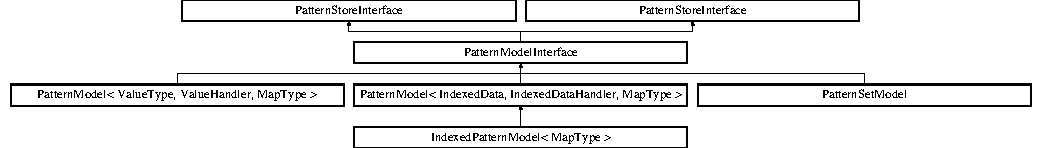
\includegraphics[height=1.206897cm]{classPatternModelInterface}
\end{center}
\end{figure}
\subsection*{Public Member Functions}
\begin{DoxyCompactItemize}
\item 
virtual int \hyperlink{classPatternModelInterface_ad485931462c2f1c1bcd0aac13ec3028b}{getmodeltype} () const  =0
\item 
virtual int \hyperlink{classPatternModelInterface_a0d58b42e55df75e04faae361677aa777}{getmodelversion} () const  =0
\item 
virtual unsigned int \hyperlink{classPatternModelInterface_afd9ec4756bb723ee6bf94321f05f1b71}{occurrencecount} (const \hyperlink{classPattern}{Pattern} \&pattern)=0
\item 
virtual double \hyperlink{classPatternModelInterface_abab22952ac502743377e3a5a524e2ae1}{frequency} (const \hyperlink{classPattern}{Pattern} \&)=0
\item 
virtual int \hyperlink{classPatternModelInterface_acbe234679e86792765d3afade8ce014c}{maxlength} () const  =0
\item 
virtual int \hyperlink{classPatternModelInterface_a53325f7b36c9cf0de4954b618eff2416}{minlength} () const  =0
\item 
virtual unsigned int \hyperlink{classPatternModelInterface_a5f3fab33835e8b01bf30b20793746e24}{types} ()=0
\item 
virtual unsigned int \hyperlink{classPatternModelInterface_aafea9a0f8fd453b85cffd18709a42ae7}{tokens} () const  =0
\item 
virtual \hyperlink{classPatternStoreInterface}{Pattern\+Store\+Interface} $\ast$ \hyperlink{classPatternModelInterface_a1bb04234bc1225becbec941a0efaa094}{getstoreinterface} ()
\item 
virtual int \hyperlink{classPatternModelInterface_ad485931462c2f1c1bcd0aac13ec3028b}{getmodeltype} () const  =0
\item 
virtual int \hyperlink{classPatternModelInterface_a0d58b42e55df75e04faae361677aa777}{getmodelversion} () const  =0
\item 
virtual unsigned int \hyperlink{classPatternModelInterface_afd9ec4756bb723ee6bf94321f05f1b71}{occurrencecount} (const \hyperlink{classPattern}{Pattern} \&pattern)=0
\item 
virtual double \hyperlink{classPatternModelInterface_abab22952ac502743377e3a5a524e2ae1}{frequency} (const \hyperlink{classPattern}{Pattern} \&)=0
\item 
virtual int \hyperlink{classPatternModelInterface_acbe234679e86792765d3afade8ce014c}{maxlength} () const  =0
\item 
virtual int \hyperlink{classPatternModelInterface_a53325f7b36c9cf0de4954b618eff2416}{minlength} () const  =0
\item 
virtual unsigned int \hyperlink{classPatternModelInterface_a5f3fab33835e8b01bf30b20793746e24}{types} ()=0
\item 
virtual unsigned int \hyperlink{classPatternModelInterface_aafea9a0f8fd453b85cffd18709a42ae7}{tokens} () const  =0
\item 
virtual \hyperlink{classPatternStoreInterface}{Pattern\+Store\+Interface} $\ast$ \hyperlink{classPatternModelInterface_a1bb04234bc1225becbec941a0efaa094}{getstoreinterface} ()
\end{DoxyCompactItemize}


\subsection{Detailed Description}
Basic read-\/only interface for pattern models, abstract base class. 

Basic read-\/only interface for pattern models, abstract base class. 

\subsection{Member Function Documentation}
\hypertarget{classPatternModelInterface_abab22952ac502743377e3a5a524e2ae1}{}\index{Pattern\+Model\+Interface@{Pattern\+Model\+Interface}!frequency@{frequency}}
\index{frequency@{frequency}!Pattern\+Model\+Interface@{Pattern\+Model\+Interface}}
\subsubsection[{frequency(const Pattern \&)=0}]{\setlength{\rightskip}{0pt plus 5cm}virtual double Pattern\+Model\+Interface\+::frequency (
\begin{DoxyParamCaption}
\item[{const {\bf Pattern} \&}]{}
\end{DoxyParamCaption}
)\hspace{0.3cm}{\ttfamily [pure virtual]}}\label{classPatternModelInterface_abab22952ac502743377e3a5a524e2ae1}
Returns the number of times the frequency of the pattern in the model, a relative/normalised value 

Implemented in \hyperlink{classPatternModel_a4ec1d0a963488d62afea4a67869758fa}{Pattern\+Model$<$ Value\+Type, Value\+Handler, Map\+Type, Pattern\+Type $>$}, \hyperlink{classPatternModel_a4ec1d0a963488d62afea4a67869758fa}{Pattern\+Model$<$ Indexed\+Data, Indexed\+Data\+Handler, Map\+Type, Pattern\+Pointer $>$}, \hyperlink{classPatternModel_a4ec1d0a963488d62afea4a67869758fa}{Pattern\+Model$<$ Indexed\+Data, Indexed\+Data\+Handler, Map\+Type, Pattern\+Type $>$}, \hyperlink{classPatternModel_a4ec1d0a963488d62afea4a67869758fa}{Pattern\+Model$<$ Value\+Type, Value\+Handler, Map\+Type, Pattern\+Pointer $>$}, and \hyperlink{classPatternSetModel_af5bdb2a283c048233e62b2a0741b7cab}{Pattern\+Set\+Model}.

\hypertarget{classPatternModelInterface_abab22952ac502743377e3a5a524e2ae1}{}\index{Pattern\+Model\+Interface@{Pattern\+Model\+Interface}!frequency@{frequency}}
\index{frequency@{frequency}!Pattern\+Model\+Interface@{Pattern\+Model\+Interface}}
\subsubsection[{frequency(const Pattern \&)=0}]{\setlength{\rightskip}{0pt plus 5cm}virtual double Pattern\+Model\+Interface\+::frequency (
\begin{DoxyParamCaption}
\item[{const {\bf Pattern} \&}]{}
\end{DoxyParamCaption}
)\hspace{0.3cm}{\ttfamily [pure virtual]}}\label{classPatternModelInterface_abab22952ac502743377e3a5a524e2ae1}
Returns the frequency of the pattern in the model, a relative/normalised value 

Implemented in \hyperlink{classPatternModel_a4ec1d0a963488d62afea4a67869758fa}{Pattern\+Model$<$ Value\+Type, Value\+Handler, Map\+Type, Pattern\+Type $>$}, \hyperlink{classPatternModel_a4ec1d0a963488d62afea4a67869758fa}{Pattern\+Model$<$ Indexed\+Data, Indexed\+Data\+Handler, Map\+Type, Pattern\+Pointer $>$}, \hyperlink{classPatternModel_a4ec1d0a963488d62afea4a67869758fa}{Pattern\+Model$<$ Indexed\+Data, Indexed\+Data\+Handler, Map\+Type, Pattern\+Type $>$}, \hyperlink{classPatternModel_a4ec1d0a963488d62afea4a67869758fa}{Pattern\+Model$<$ Value\+Type, Value\+Handler, Map\+Type, Pattern\+Pointer $>$}, and \hyperlink{classPatternSetModel_af5bdb2a283c048233e62b2a0741b7cab}{Pattern\+Set\+Model}.

\hypertarget{classPatternModelInterface_ad485931462c2f1c1bcd0aac13ec3028b}{}\index{Pattern\+Model\+Interface@{Pattern\+Model\+Interface}!getmodeltype@{getmodeltype}}
\index{getmodeltype@{getmodeltype}!Pattern\+Model\+Interface@{Pattern\+Model\+Interface}}
\subsubsection[{getmodeltype() const  =0}]{\setlength{\rightskip}{0pt plus 5cm}virtual int Pattern\+Model\+Interface\+::getmodeltype (
\begin{DoxyParamCaption}
{}
\end{DoxyParamCaption}
) const\hspace{0.3cm}{\ttfamily [pure virtual]}}\label{classPatternModelInterface_ad485931462c2f1c1bcd0aac13ec3028b}
Get the type of the model \begin{DoxyReturn}{Returns}
Model\+Type 
\end{DoxyReturn}


Implemented in \hyperlink{classIndexedPatternPointerModel_a2cf62012c68c8557403226ff478500e9}{Indexed\+Pattern\+Pointer\+Model$<$ Map\+Type $>$}, \hyperlink{classPatternPointerModel_a6588706e670ebd3b14e2ab71c19011b7}{Pattern\+Pointer\+Model$<$ Value\+Type, Value\+Handler, Map\+Type $>$}, \hyperlink{classIndexedPatternModel_a63f42808d22dd3a813242332ad42ee6c}{Indexed\+Pattern\+Model$<$ Map\+Type, Pattern\+Type $>$}, \hyperlink{classIndexedPatternModel_a63f42808d22dd3a813242332ad42ee6c}{Indexed\+Pattern\+Model$<$ Map\+Type, Pattern\+Pointer $>$}, \hyperlink{classPatternModel_ac4a38270c6a2dbcfccf0b8baebee11eb}{Pattern\+Model$<$ Value\+Type, Value\+Handler, Map\+Type, Pattern\+Type $>$}, \hyperlink{classPatternModel_ac4a38270c6a2dbcfccf0b8baebee11eb}{Pattern\+Model$<$ Indexed\+Data, Indexed\+Data\+Handler, Map\+Type, Pattern\+Pointer $>$}, \hyperlink{classPatternModel_ac4a38270c6a2dbcfccf0b8baebee11eb}{Pattern\+Model$<$ Indexed\+Data, Indexed\+Data\+Handler, Map\+Type, Pattern\+Type $>$}, \hyperlink{classPatternModel_ac4a38270c6a2dbcfccf0b8baebee11eb}{Pattern\+Model$<$ Value\+Type, Value\+Handler, Map\+Type, Pattern\+Pointer $>$}, and \hyperlink{classPatternSetModel_a27adf3033f15f03e908d53d032779d09}{Pattern\+Set\+Model}.

\hypertarget{classPatternModelInterface_ad485931462c2f1c1bcd0aac13ec3028b}{}\index{Pattern\+Model\+Interface@{Pattern\+Model\+Interface}!getmodeltype@{getmodeltype}}
\index{getmodeltype@{getmodeltype}!Pattern\+Model\+Interface@{Pattern\+Model\+Interface}}
\subsubsection[{getmodeltype() const  =0}]{\setlength{\rightskip}{0pt plus 5cm}virtual int Pattern\+Model\+Interface\+::getmodeltype (
\begin{DoxyParamCaption}
{}
\end{DoxyParamCaption}
) const\hspace{0.3cm}{\ttfamily [pure virtual]}}\label{classPatternModelInterface_ad485931462c2f1c1bcd0aac13ec3028b}
Get the type of the model \begin{DoxyReturn}{Returns}
Model\+Type 
\end{DoxyReturn}


Implemented in \hyperlink{classIndexedPatternPointerModel_a2cf62012c68c8557403226ff478500e9}{Indexed\+Pattern\+Pointer\+Model$<$ Map\+Type $>$}, \hyperlink{classPatternPointerModel_a6588706e670ebd3b14e2ab71c19011b7}{Pattern\+Pointer\+Model$<$ Value\+Type, Value\+Handler, Map\+Type $>$}, \hyperlink{classIndexedPatternModel_a63f42808d22dd3a813242332ad42ee6c}{Indexed\+Pattern\+Model$<$ Map\+Type, Pattern\+Type $>$}, \hyperlink{classIndexedPatternModel_a63f42808d22dd3a813242332ad42ee6c}{Indexed\+Pattern\+Model$<$ Map\+Type, Pattern\+Pointer $>$}, \hyperlink{classPatternModel_ac4a38270c6a2dbcfccf0b8baebee11eb}{Pattern\+Model$<$ Value\+Type, Value\+Handler, Map\+Type, Pattern\+Type $>$}, \hyperlink{classPatternModel_ac4a38270c6a2dbcfccf0b8baebee11eb}{Pattern\+Model$<$ Indexed\+Data, Indexed\+Data\+Handler, Map\+Type, Pattern\+Pointer $>$}, \hyperlink{classPatternModel_ac4a38270c6a2dbcfccf0b8baebee11eb}{Pattern\+Model$<$ Indexed\+Data, Indexed\+Data\+Handler, Map\+Type, Pattern\+Type $>$}, \hyperlink{classPatternModel_ac4a38270c6a2dbcfccf0b8baebee11eb}{Pattern\+Model$<$ Value\+Type, Value\+Handler, Map\+Type, Pattern\+Pointer $>$}, and \hyperlink{classPatternSetModel_a27adf3033f15f03e908d53d032779d09}{Pattern\+Set\+Model}.

\hypertarget{classPatternModelInterface_a0d58b42e55df75e04faae361677aa777}{}\index{Pattern\+Model\+Interface@{Pattern\+Model\+Interface}!getmodelversion@{getmodelversion}}
\index{getmodelversion@{getmodelversion}!Pattern\+Model\+Interface@{Pattern\+Model\+Interface}}
\subsubsection[{getmodelversion() const  =0}]{\setlength{\rightskip}{0pt plus 5cm}virtual int Pattern\+Model\+Interface\+::getmodelversion (
\begin{DoxyParamCaption}
{}
\end{DoxyParamCaption}
) const\hspace{0.3cm}{\ttfamily [pure virtual]}}\label{classPatternModelInterface_a0d58b42e55df75e04faae361677aa777}
Get the version number of the model 

Implemented in \hyperlink{classIndexedPatternPointerModel_a34a68ddd193a441242b8d24fca7392b8}{Indexed\+Pattern\+Pointer\+Model$<$ Map\+Type $>$}, \hyperlink{classPatternPointerModel_a84979d2ff5033607dba04bb2210108d2}{Pattern\+Pointer\+Model$<$ Value\+Type, Value\+Handler, Map\+Type $>$}, \hyperlink{classIndexedPatternModel_a50e185e2f7e48751f8633d4b981089bc}{Indexed\+Pattern\+Model$<$ Map\+Type, Pattern\+Type $>$}, \hyperlink{classIndexedPatternModel_a50e185e2f7e48751f8633d4b981089bc}{Indexed\+Pattern\+Model$<$ Map\+Type, Pattern\+Pointer $>$}, \hyperlink{classPatternModel_a760a01e32f97b63400d13e69384dad86}{Pattern\+Model$<$ Value\+Type, Value\+Handler, Map\+Type, Pattern\+Type $>$}, \hyperlink{classPatternModel_a760a01e32f97b63400d13e69384dad86}{Pattern\+Model$<$ Indexed\+Data, Indexed\+Data\+Handler, Map\+Type, Pattern\+Pointer $>$}, \hyperlink{classPatternModel_a760a01e32f97b63400d13e69384dad86}{Pattern\+Model$<$ Indexed\+Data, Indexed\+Data\+Handler, Map\+Type, Pattern\+Type $>$}, \hyperlink{classPatternModel_a760a01e32f97b63400d13e69384dad86}{Pattern\+Model$<$ Value\+Type, Value\+Handler, Map\+Type, Pattern\+Pointer $>$}, and \hyperlink{classPatternSetModel_a79dc7fd04e3de5eb894541bd664f5d12}{Pattern\+Set\+Model}.

\hypertarget{classPatternModelInterface_a0d58b42e55df75e04faae361677aa777}{}\index{Pattern\+Model\+Interface@{Pattern\+Model\+Interface}!getmodelversion@{getmodelversion}}
\index{getmodelversion@{getmodelversion}!Pattern\+Model\+Interface@{Pattern\+Model\+Interface}}
\subsubsection[{getmodelversion() const  =0}]{\setlength{\rightskip}{0pt plus 5cm}virtual int Pattern\+Model\+Interface\+::getmodelversion (
\begin{DoxyParamCaption}
{}
\end{DoxyParamCaption}
) const\hspace{0.3cm}{\ttfamily [pure virtual]}}\label{classPatternModelInterface_a0d58b42e55df75e04faae361677aa777}
Get the version number of the model 

Implemented in \hyperlink{classIndexedPatternPointerModel_a34a68ddd193a441242b8d24fca7392b8}{Indexed\+Pattern\+Pointer\+Model$<$ Map\+Type $>$}, \hyperlink{classPatternPointerModel_a84979d2ff5033607dba04bb2210108d2}{Pattern\+Pointer\+Model$<$ Value\+Type, Value\+Handler, Map\+Type $>$}, \hyperlink{classIndexedPatternModel_a50e185e2f7e48751f8633d4b981089bc}{Indexed\+Pattern\+Model$<$ Map\+Type, Pattern\+Type $>$}, \hyperlink{classIndexedPatternModel_a50e185e2f7e48751f8633d4b981089bc}{Indexed\+Pattern\+Model$<$ Map\+Type, Pattern\+Pointer $>$}, \hyperlink{classPatternModel_a760a01e32f97b63400d13e69384dad86}{Pattern\+Model$<$ Value\+Type, Value\+Handler, Map\+Type, Pattern\+Type $>$}, \hyperlink{classPatternModel_a760a01e32f97b63400d13e69384dad86}{Pattern\+Model$<$ Indexed\+Data, Indexed\+Data\+Handler, Map\+Type, Pattern\+Pointer $>$}, \hyperlink{classPatternModel_a760a01e32f97b63400d13e69384dad86}{Pattern\+Model$<$ Indexed\+Data, Indexed\+Data\+Handler, Map\+Type, Pattern\+Type $>$}, \hyperlink{classPatternModel_a760a01e32f97b63400d13e69384dad86}{Pattern\+Model$<$ Value\+Type, Value\+Handler, Map\+Type, Pattern\+Pointer $>$}, and \hyperlink{classPatternSetModel_a79dc7fd04e3de5eb894541bd664f5d12}{Pattern\+Set\+Model}.

\hypertarget{classPatternModelInterface_a1bb04234bc1225becbec941a0efaa094}{}\index{Pattern\+Model\+Interface@{Pattern\+Model\+Interface}!getstoreinterface@{getstoreinterface}}
\index{getstoreinterface@{getstoreinterface}!Pattern\+Model\+Interface@{Pattern\+Model\+Interface}}
\subsubsection[{getstoreinterface()}]{\setlength{\rightskip}{0pt plus 5cm}virtual {\bf Pattern\+Store\+Interface}$\ast$ Pattern\+Model\+Interface\+::getstoreinterface (
\begin{DoxyParamCaption}
{}
\end{DoxyParamCaption}
)\hspace{0.3cm}{\ttfamily [inline]}, {\ttfamily [virtual]}}\label{classPatternModelInterface_a1bb04234bc1225becbec941a0efaa094}
\hypertarget{classPatternModelInterface_a1bb04234bc1225becbec941a0efaa094}{}\index{Pattern\+Model\+Interface@{Pattern\+Model\+Interface}!getstoreinterface@{getstoreinterface}}
\index{getstoreinterface@{getstoreinterface}!Pattern\+Model\+Interface@{Pattern\+Model\+Interface}}
\subsubsection[{getstoreinterface()}]{\setlength{\rightskip}{0pt plus 5cm}virtual {\bf Pattern\+Store\+Interface}$\ast$ Pattern\+Model\+Interface\+::getstoreinterface (
\begin{DoxyParamCaption}
{}
\end{DoxyParamCaption}
)\hspace{0.3cm}{\ttfamily [inline]}, {\ttfamily [virtual]}}\label{classPatternModelInterface_a1bb04234bc1225becbec941a0efaa094}
\hypertarget{classPatternModelInterface_acbe234679e86792765d3afade8ce014c}{}\index{Pattern\+Model\+Interface@{Pattern\+Model\+Interface}!maxlength@{maxlength}}
\index{maxlength@{maxlength}!Pattern\+Model\+Interface@{Pattern\+Model\+Interface}}
\subsubsection[{maxlength() const  =0}]{\setlength{\rightskip}{0pt plus 5cm}virtual int Pattern\+Model\+Interface\+::maxlength (
\begin{DoxyParamCaption}
{}
\end{DoxyParamCaption}
) const\hspace{0.3cm}{\ttfamily [pure virtual]}}\label{classPatternModelInterface_acbe234679e86792765d3afade8ce014c}
Return the maximum pattern length in this model 

Implemented in \hyperlink{classPatternModel_a545fbfefef4eadb268217ec781c494bb}{Pattern\+Model$<$ Value\+Type, Value\+Handler, Map\+Type, Pattern\+Type $>$}, \hyperlink{classPatternModel_a545fbfefef4eadb268217ec781c494bb}{Pattern\+Model$<$ Indexed\+Data, Indexed\+Data\+Handler, Map\+Type, Pattern\+Pointer $>$}, \hyperlink{classPatternModel_a545fbfefef4eadb268217ec781c494bb}{Pattern\+Model$<$ Indexed\+Data, Indexed\+Data\+Handler, Map\+Type, Pattern\+Type $>$}, \hyperlink{classPatternModel_a545fbfefef4eadb268217ec781c494bb}{Pattern\+Model$<$ Value\+Type, Value\+Handler, Map\+Type, Pattern\+Pointer $>$}, and \hyperlink{classPatternSetModel_abd386cc901e2328079a349eae42d9ee8}{Pattern\+Set\+Model}.

\hypertarget{classPatternModelInterface_acbe234679e86792765d3afade8ce014c}{}\index{Pattern\+Model\+Interface@{Pattern\+Model\+Interface}!maxlength@{maxlength}}
\index{maxlength@{maxlength}!Pattern\+Model\+Interface@{Pattern\+Model\+Interface}}
\subsubsection[{maxlength() const  =0}]{\setlength{\rightskip}{0pt plus 5cm}virtual int Pattern\+Model\+Interface\+::maxlength (
\begin{DoxyParamCaption}
{}
\end{DoxyParamCaption}
) const\hspace{0.3cm}{\ttfamily [pure virtual]}}\label{classPatternModelInterface_acbe234679e86792765d3afade8ce014c}
Return the maximum pattern length in this model 

Implemented in \hyperlink{classPatternModel_a545fbfefef4eadb268217ec781c494bb}{Pattern\+Model$<$ Value\+Type, Value\+Handler, Map\+Type, Pattern\+Type $>$}, \hyperlink{classPatternModel_a545fbfefef4eadb268217ec781c494bb}{Pattern\+Model$<$ Indexed\+Data, Indexed\+Data\+Handler, Map\+Type, Pattern\+Pointer $>$}, \hyperlink{classPatternModel_a545fbfefef4eadb268217ec781c494bb}{Pattern\+Model$<$ Indexed\+Data, Indexed\+Data\+Handler, Map\+Type, Pattern\+Type $>$}, \hyperlink{classPatternModel_a545fbfefef4eadb268217ec781c494bb}{Pattern\+Model$<$ Value\+Type, Value\+Handler, Map\+Type, Pattern\+Pointer $>$}, and \hyperlink{classPatternSetModel_abd386cc901e2328079a349eae42d9ee8}{Pattern\+Set\+Model}.

\hypertarget{classPatternModelInterface_a53325f7b36c9cf0de4954b618eff2416}{}\index{Pattern\+Model\+Interface@{Pattern\+Model\+Interface}!minlength@{minlength}}
\index{minlength@{minlength}!Pattern\+Model\+Interface@{Pattern\+Model\+Interface}}
\subsubsection[{minlength() const  =0}]{\setlength{\rightskip}{0pt plus 5cm}virtual int Pattern\+Model\+Interface\+::minlength (
\begin{DoxyParamCaption}
{}
\end{DoxyParamCaption}
) const\hspace{0.3cm}{\ttfamily [pure virtual]}}\label{classPatternModelInterface_a53325f7b36c9cf0de4954b618eff2416}
Returns the minumum pattern length in this model 

Implemented in \hyperlink{classPatternModel_a7a0208745487928ecb418baeb78e810f}{Pattern\+Model$<$ Value\+Type, Value\+Handler, Map\+Type, Pattern\+Type $>$}, \hyperlink{classPatternModel_a7a0208745487928ecb418baeb78e810f}{Pattern\+Model$<$ Indexed\+Data, Indexed\+Data\+Handler, Map\+Type, Pattern\+Pointer $>$}, \hyperlink{classPatternModel_a7a0208745487928ecb418baeb78e810f}{Pattern\+Model$<$ Indexed\+Data, Indexed\+Data\+Handler, Map\+Type, Pattern\+Type $>$}, \hyperlink{classPatternModel_a7a0208745487928ecb418baeb78e810f}{Pattern\+Model$<$ Value\+Type, Value\+Handler, Map\+Type, Pattern\+Pointer $>$}, and \hyperlink{classPatternSetModel_a3cc6ca22d4dd68270068d5a4e05f530a}{Pattern\+Set\+Model}.

\hypertarget{classPatternModelInterface_a53325f7b36c9cf0de4954b618eff2416}{}\index{Pattern\+Model\+Interface@{Pattern\+Model\+Interface}!minlength@{minlength}}
\index{minlength@{minlength}!Pattern\+Model\+Interface@{Pattern\+Model\+Interface}}
\subsubsection[{minlength() const  =0}]{\setlength{\rightskip}{0pt plus 5cm}virtual int Pattern\+Model\+Interface\+::minlength (
\begin{DoxyParamCaption}
{}
\end{DoxyParamCaption}
) const\hspace{0.3cm}{\ttfamily [pure virtual]}}\label{classPatternModelInterface_a53325f7b36c9cf0de4954b618eff2416}
Returns the minumum pattern length in this model 

Implemented in \hyperlink{classPatternModel_a7a0208745487928ecb418baeb78e810f}{Pattern\+Model$<$ Value\+Type, Value\+Handler, Map\+Type, Pattern\+Type $>$}, \hyperlink{classPatternModel_a7a0208745487928ecb418baeb78e810f}{Pattern\+Model$<$ Indexed\+Data, Indexed\+Data\+Handler, Map\+Type, Pattern\+Pointer $>$}, \hyperlink{classPatternModel_a7a0208745487928ecb418baeb78e810f}{Pattern\+Model$<$ Indexed\+Data, Indexed\+Data\+Handler, Map\+Type, Pattern\+Type $>$}, \hyperlink{classPatternModel_a7a0208745487928ecb418baeb78e810f}{Pattern\+Model$<$ Value\+Type, Value\+Handler, Map\+Type, Pattern\+Pointer $>$}, and \hyperlink{classPatternSetModel_a3cc6ca22d4dd68270068d5a4e05f530a}{Pattern\+Set\+Model}.

\hypertarget{classPatternModelInterface_afd9ec4756bb723ee6bf94321f05f1b71}{}\index{Pattern\+Model\+Interface@{Pattern\+Model\+Interface}!occurrencecount@{occurrencecount}}
\index{occurrencecount@{occurrencecount}!Pattern\+Model\+Interface@{Pattern\+Model\+Interface}}
\subsubsection[{occurrencecount(const Pattern \&pattern)=0}]{\setlength{\rightskip}{0pt plus 5cm}virtual unsigned int Pattern\+Model\+Interface\+::occurrencecount (
\begin{DoxyParamCaption}
\item[{const {\bf Pattern} \&}]{pattern}
\end{DoxyParamCaption}
)\hspace{0.3cm}{\ttfamily [pure virtual]}}\label{classPatternModelInterface_afd9ec4756bb723ee6bf94321f05f1b71}
Returns the number of times this pattern occurs in the model 

Implemented in \hyperlink{classPatternModel_a013725360804aac3514eb8bb436102db}{Pattern\+Model$<$ Value\+Type, Value\+Handler, Map\+Type, Pattern\+Type $>$}, \hyperlink{classPatternModel_a013725360804aac3514eb8bb436102db}{Pattern\+Model$<$ Indexed\+Data, Indexed\+Data\+Handler, Map\+Type, Pattern\+Pointer $>$}, \hyperlink{classPatternModel_a013725360804aac3514eb8bb436102db}{Pattern\+Model$<$ Indexed\+Data, Indexed\+Data\+Handler, Map\+Type, Pattern\+Type $>$}, \hyperlink{classPatternModel_a013725360804aac3514eb8bb436102db}{Pattern\+Model$<$ Value\+Type, Value\+Handler, Map\+Type, Pattern\+Pointer $>$}, and \hyperlink{classPatternSetModel_ab1ca42eb82df349263b10c57f968678e}{Pattern\+Set\+Model}.

\hypertarget{classPatternModelInterface_afd9ec4756bb723ee6bf94321f05f1b71}{}\index{Pattern\+Model\+Interface@{Pattern\+Model\+Interface}!occurrencecount@{occurrencecount}}
\index{occurrencecount@{occurrencecount}!Pattern\+Model\+Interface@{Pattern\+Model\+Interface}}
\subsubsection[{occurrencecount(const Pattern \&pattern)=0}]{\setlength{\rightskip}{0pt plus 5cm}virtual unsigned int Pattern\+Model\+Interface\+::occurrencecount (
\begin{DoxyParamCaption}
\item[{const {\bf Pattern} \&}]{pattern}
\end{DoxyParamCaption}
)\hspace{0.3cm}{\ttfamily [pure virtual]}}\label{classPatternModelInterface_afd9ec4756bb723ee6bf94321f05f1b71}
Returns the number of times this pattern occurs in the model 

Implemented in \hyperlink{classPatternModel_a013725360804aac3514eb8bb436102db}{Pattern\+Model$<$ Value\+Type, Value\+Handler, Map\+Type, Pattern\+Type $>$}, \hyperlink{classPatternModel_a013725360804aac3514eb8bb436102db}{Pattern\+Model$<$ Indexed\+Data, Indexed\+Data\+Handler, Map\+Type, Pattern\+Pointer $>$}, \hyperlink{classPatternModel_a013725360804aac3514eb8bb436102db}{Pattern\+Model$<$ Indexed\+Data, Indexed\+Data\+Handler, Map\+Type, Pattern\+Type $>$}, \hyperlink{classPatternModel_a013725360804aac3514eb8bb436102db}{Pattern\+Model$<$ Value\+Type, Value\+Handler, Map\+Type, Pattern\+Pointer $>$}, and \hyperlink{classPatternSetModel_ab1ca42eb82df349263b10c57f968678e}{Pattern\+Set\+Model}.

\hypertarget{classPatternModelInterface_aafea9a0f8fd453b85cffd18709a42ae7}{}\index{Pattern\+Model\+Interface@{Pattern\+Model\+Interface}!tokens@{tokens}}
\index{tokens@{tokens}!Pattern\+Model\+Interface@{Pattern\+Model\+Interface}}
\subsubsection[{tokens() const  =0}]{\setlength{\rightskip}{0pt plus 5cm}virtual unsigned int Pattern\+Model\+Interface\+::tokens (
\begin{DoxyParamCaption}
{}
\end{DoxyParamCaption}
) const\hspace{0.3cm}{\ttfamily [pure virtual]}}\label{classPatternModelInterface_aafea9a0f8fd453b85cffd18709a42ae7}
Returns the number of tokens in the original corpus, includes tokens not covered by the model! 

Implemented in \hyperlink{classPatternModel_a9e4a67d7c0136f9c9a8da56df5ffc18c}{Pattern\+Model$<$ Value\+Type, Value\+Handler, Map\+Type, Pattern\+Type $>$}, \hyperlink{classPatternModel_a9e4a67d7c0136f9c9a8da56df5ffc18c}{Pattern\+Model$<$ Indexed\+Data, Indexed\+Data\+Handler, Map\+Type, Pattern\+Pointer $>$}, \hyperlink{classPatternModel_a9e4a67d7c0136f9c9a8da56df5ffc18c}{Pattern\+Model$<$ Indexed\+Data, Indexed\+Data\+Handler, Map\+Type, Pattern\+Type $>$}, \hyperlink{classPatternModel_a9e4a67d7c0136f9c9a8da56df5ffc18c}{Pattern\+Model$<$ Value\+Type, Value\+Handler, Map\+Type, Pattern\+Pointer $>$}, and \hyperlink{classPatternSetModel_aa834dd6a5467ea8a68680512d6251e16}{Pattern\+Set\+Model}.

\hypertarget{classPatternModelInterface_aafea9a0f8fd453b85cffd18709a42ae7}{}\index{Pattern\+Model\+Interface@{Pattern\+Model\+Interface}!tokens@{tokens}}
\index{tokens@{tokens}!Pattern\+Model\+Interface@{Pattern\+Model\+Interface}}
\subsubsection[{tokens() const  =0}]{\setlength{\rightskip}{0pt plus 5cm}virtual unsigned int Pattern\+Model\+Interface\+::tokens (
\begin{DoxyParamCaption}
{}
\end{DoxyParamCaption}
) const\hspace{0.3cm}{\ttfamily [pure virtual]}}\label{classPatternModelInterface_aafea9a0f8fd453b85cffd18709a42ae7}
Returns the number of tokens in the original corpus, includes tokens not covered by the model! 

Implemented in \hyperlink{classPatternModel_a9e4a67d7c0136f9c9a8da56df5ffc18c}{Pattern\+Model$<$ Value\+Type, Value\+Handler, Map\+Type, Pattern\+Type $>$}, \hyperlink{classPatternModel_a9e4a67d7c0136f9c9a8da56df5ffc18c}{Pattern\+Model$<$ Indexed\+Data, Indexed\+Data\+Handler, Map\+Type, Pattern\+Pointer $>$}, \hyperlink{classPatternModel_a9e4a67d7c0136f9c9a8da56df5ffc18c}{Pattern\+Model$<$ Indexed\+Data, Indexed\+Data\+Handler, Map\+Type, Pattern\+Type $>$}, \hyperlink{classPatternModel_a9e4a67d7c0136f9c9a8da56df5ffc18c}{Pattern\+Model$<$ Value\+Type, Value\+Handler, Map\+Type, Pattern\+Pointer $>$}, and \hyperlink{classPatternSetModel_aa834dd6a5467ea8a68680512d6251e16}{Pattern\+Set\+Model}.

\hypertarget{classPatternModelInterface_a5f3fab33835e8b01bf30b20793746e24}{}\index{Pattern\+Model\+Interface@{Pattern\+Model\+Interface}!types@{types}}
\index{types@{types}!Pattern\+Model\+Interface@{Pattern\+Model\+Interface}}
\subsubsection[{types()=0}]{\setlength{\rightskip}{0pt plus 5cm}virtual unsigned int Pattern\+Model\+Interface\+::types (
\begin{DoxyParamCaption}
{}
\end{DoxyParamCaption}
)\hspace{0.3cm}{\ttfamily [pure virtual]}}\label{classPatternModelInterface_a5f3fab33835e8b01bf30b20793746e24}
Return the number of distinct words/unigram in the original corpus, includes types not covered by the model! 

Implemented in \hyperlink{classPatternModel_a6e5ac4583443112eb1a78157aed967b5}{Pattern\+Model$<$ Value\+Type, Value\+Handler, Map\+Type, Pattern\+Type $>$}, \hyperlink{classPatternModel_a6e5ac4583443112eb1a78157aed967b5}{Pattern\+Model$<$ Indexed\+Data, Indexed\+Data\+Handler, Map\+Type, Pattern\+Pointer $>$}, \hyperlink{classPatternModel_a6e5ac4583443112eb1a78157aed967b5}{Pattern\+Model$<$ Indexed\+Data, Indexed\+Data\+Handler, Map\+Type, Pattern\+Type $>$}, \hyperlink{classPatternModel_a6e5ac4583443112eb1a78157aed967b5}{Pattern\+Model$<$ Value\+Type, Value\+Handler, Map\+Type, Pattern\+Pointer $>$}, and \hyperlink{classPatternSetModel_a178d3c988a43130b4ba3d4fa57001055}{Pattern\+Set\+Model}.

\hypertarget{classPatternModelInterface_a5f3fab33835e8b01bf30b20793746e24}{}\index{Pattern\+Model\+Interface@{Pattern\+Model\+Interface}!types@{types}}
\index{types@{types}!Pattern\+Model\+Interface@{Pattern\+Model\+Interface}}
\subsubsection[{types()=0}]{\setlength{\rightskip}{0pt plus 5cm}virtual unsigned int Pattern\+Model\+Interface\+::types (
\begin{DoxyParamCaption}
{}
\end{DoxyParamCaption}
)\hspace{0.3cm}{\ttfamily [pure virtual]}}\label{classPatternModelInterface_a5f3fab33835e8b01bf30b20793746e24}
Return the number of distinct words/unigram in the original corpus, includes types not covered by the model! 

Implemented in \hyperlink{classPatternModel_a6e5ac4583443112eb1a78157aed967b5}{Pattern\+Model$<$ Value\+Type, Value\+Handler, Map\+Type, Pattern\+Type $>$}, \hyperlink{classPatternModel_a6e5ac4583443112eb1a78157aed967b5}{Pattern\+Model$<$ Indexed\+Data, Indexed\+Data\+Handler, Map\+Type, Pattern\+Pointer $>$}, \hyperlink{classPatternModel_a6e5ac4583443112eb1a78157aed967b5}{Pattern\+Model$<$ Indexed\+Data, Indexed\+Data\+Handler, Map\+Type, Pattern\+Type $>$}, \hyperlink{classPatternModel_a6e5ac4583443112eb1a78157aed967b5}{Pattern\+Model$<$ Value\+Type, Value\+Handler, Map\+Type, Pattern\+Pointer $>$}, and \hyperlink{classPatternSetModel_a178d3c988a43130b4ba3d4fa57001055}{Pattern\+Set\+Model}.



The documentation for this class was generated from the following files\+:\begin{DoxyCompactItemize}
\item 
include/\hyperlink{interface_8h}{interface.\+h}\item 
include/\hyperlink{patternmodel_8h}{patternmodel.\+h}\end{DoxyCompactItemize}

\hypertarget{classPatternModelOptions}{}\section{Pattern\+Model\+Options Class Reference}
\label{classPatternModelOptions}\index{Pattern\+Model\+Options@{Pattern\+Model\+Options}}


Options for \hyperlink{classPattern}{Pattern} Model loading and training.  




{\ttfamily \#include $<$patternmodel.\+h$>$}

\subsection*{Public Member Functions}
\begin{DoxyCompactItemize}
\item 
\hyperlink{classPatternModelOptions_a32b803262231539a8cd3d715dea7ee81}{Pattern\+Model\+Options} ()
\item 
\hyperlink{classPatternModelOptions_a4166fddbf1270f94c60d1c5f391972a9}{Pattern\+Model\+Options} (const \hyperlink{classPatternModelOptions}{Pattern\+Model\+Options} \&ref)
\end{DoxyCompactItemize}
\subsection*{Public Attributes}
\begin{DoxyCompactItemize}
\item 
int \hyperlink{classPatternModelOptions_a4572cfbca28c3130d98f886a4c1857e0}{M\+I\+N\+T\+O\+K\+E\+N\+S}
\item 
int \hyperlink{classPatternModelOptions_a130b2214a2a9eaaa4862f8019fdfe2bc}{M\+I\+N\+T\+O\+K\+E\+N\+S\+\_\+\+S\+K\+I\+P\+G\+R\+A\+M\+S}
\item 
int \hyperlink{classPatternModelOptions_a14d2ed1c3edb2c9b3944aff462e87a03}{M\+I\+N\+T\+O\+K\+E\+N\+S\+\_\+\+U\+N\+I\+G\+R\+A\+M\+S}
\item 
int \hyperlink{classPatternModelOptions_a4dada20f1bba3cc5e08a49e4a9bfb545}{M\+I\+N\+L\+E\+N\+G\+T\+H}
\begin{DoxyCompactList}\small\item\em The minimum length of patterns to be loaded/extracted (in words/tokens) (default\+: 1) \end{DoxyCompactList}\item 
int \hyperlink{classPatternModelOptions_a7630da974c460ec2d67c2ed9f4c84144}{M\+A\+X\+L\+E\+N\+G\+T\+H}
\begin{DoxyCompactList}\small\item\em The maximum length of patterns to be loaded/extracted, inclusive (in words/tokens) (default\+: 100) \end{DoxyCompactList}\item 
int \hyperlink{classPatternModelOptions_a9154b55890ee1ff5d9ec43741a0e3908}{M\+A\+X\+B\+A\+C\+K\+O\+F\+F\+L\+E\+N\+G\+T\+H}
\item 
bool \hyperlink{classPatternModelOptions_a79465fd9abbfab5a481222d9660e598a}{D\+O\+S\+K\+I\+P\+G\+R\+A\+M\+S}
\begin{DoxyCompactList}\small\item\em Load/extract skipgrams? (default\+: false) \end{DoxyCompactList}\item 
bool \hyperlink{classPatternModelOptions_ab9f8da4d9fe653cf967f571ae6766ed4}{D\+O\+S\+K\+I\+P\+G\+R\+A\+M\+S\+\_\+\+E\+X\+H\+A\+U\+S\+T\+I\+V\+E}
\begin{DoxyCompactList}\small\item\em Load/extract skipgrams in an exhaustive fashion? More memory intensive, but the only options for unindexed models (default\+: false) \end{DoxyCompactList}\item 
int \hyperlink{classPatternModelOptions_ad5b2686b6f641463c54441a595259046}{M\+I\+N\+S\+K\+I\+P\+T\+Y\+P\+E\+S}
\begin{DoxyCompactList}\small\item\em Minimum required amount of distinct patterns that can fit in a gap of a skipgram for the skipgram to be included (default\+: 2) \end{DoxyCompactList}\item 
bool \hyperlink{classPatternModelOptions_ad4d4b2fa96e3355b9e3f4b8e51bb62ff}{D\+O\+R\+E\+V\+E\+R\+S\+E\+I\+N\+D\+E\+X}
\begin{DoxyCompactList}\small\item\em Compute reverse index? Costs memory. This will be way faster when you pass an \hyperlink{classIndexedCorpus}{Indexed\+Corpus} to the \hyperlink{classPatternModel}{Pattern\+Model} constructor. (default\+: true) \end{DoxyCompactList}\item 
bool \hyperlink{classPatternModelOptions_ad4391604983decec050de83f13cd6235}{D\+O\+P\+A\+T\+T\+E\+R\+N\+P\+E\+R\+L\+I\+N\+E}
\begin{DoxyCompactList}\small\item\em Assume each line contains one integral pattern, rather than actively extracting all subpatterns on a line (default\+: false) \end{DoxyCompactList}\item 
int \hyperlink{classPatternModelOptions_acb220b576d5b4126289cd4a6dec98a1c}{P\+R\+U\+N\+E\+N\+O\+N\+S\+U\+B\+S\+U\+M\+E\+D}
\item 
bool \hyperlink{classPatternModelOptions_ad7c8615dee16492c719bf455bb67e6a5}{D\+O\+R\+E\+M\+O\+V\+E\+I\+N\+D\+E\+X}
\begin{DoxyCompactList}\small\item\em Do not load index information (for indexed models), loads just the patterns without any counts. \end{DoxyCompactList}\item 
bool \hyperlink{classPatternModelOptions_a4ded839cdeb4f4191896d074ef45cf6e}{D\+O\+R\+E\+M\+O\+V\+E\+N\+G\+R\+A\+M\+S}
\begin{DoxyCompactList}\small\item\em Remove n-\/grams from the model upon loading it. \end{DoxyCompactList}\item 
bool \hyperlink{classPatternModelOptions_a88eb47abf2e38a2afac00e8cb9a7a869}{D\+O\+R\+E\+M\+O\+V\+E\+S\+K\+I\+P\+G\+R\+A\+M\+S}
\begin{DoxyCompactList}\small\item\em Remove skip-\/grams from the model upon loading it. \end{DoxyCompactList}\item 
bool \hyperlink{classPatternModelOptions_a82fad4131fd2b0a41a81f65586ae9378}{D\+O\+R\+E\+M\+O\+V\+E\+F\+L\+E\+X\+G\+R\+A\+M\+S}
\begin{DoxyCompactList}\small\item\em Remove flexgrams from the model upon loading it. \end{DoxyCompactList}\item 
bool \hyperlink{classPatternModelOptions_a52b76b6c81b7666c997ca05bc1df7e97}{D\+O\+R\+E\+S\+E\+T}
\begin{DoxyCompactList}\small\item\em sets all counts to zero upon loading, clears indices \end{DoxyCompactList}\item 
bool \hyperlink{classPatternModelOptions_ad99d007239e6ef18a6fd8ce51fb9d1bd}{Q\+U\+I\+E\+T}
\begin{DoxyCompactList}\small\item\em Don\textquotesingle{}t output to stderr. \end{DoxyCompactList}\item 
bool \hyperlink{classPatternModelOptions_ae0019dce9d441e011dab04dea4fa8d46}{D\+E\+B\+U\+G}
\begin{DoxyCompactList}\small\item\em Output extra debug information. \end{DoxyCompactList}\end{DoxyCompactItemize}


\subsection{Detailed Description}
Options for \hyperlink{classPattern}{Pattern} Model loading and training. 

This class defines all kinds of parameters that can be set for loading and training \hyperlink{classPattern}{Pattern} Models, it is passed to various constructors and methods. 

\subsection{Constructor \& Destructor Documentation}
\hypertarget{classPatternModelOptions_a32b803262231539a8cd3d715dea7ee81}{}\index{Pattern\+Model\+Options@{Pattern\+Model\+Options}!Pattern\+Model\+Options@{Pattern\+Model\+Options}}
\index{Pattern\+Model\+Options@{Pattern\+Model\+Options}!Pattern\+Model\+Options@{Pattern\+Model\+Options}}
\subsubsection[{Pattern\+Model\+Options()}]{\setlength{\rightskip}{0pt plus 5cm}Pattern\+Model\+Options\+::\+Pattern\+Model\+Options (
\begin{DoxyParamCaption}
{}
\end{DoxyParamCaption}
)\hspace{0.3cm}{\ttfamily [inline]}}\label{classPatternModelOptions_a32b803262231539a8cd3d715dea7ee81}
Initialise with default values. All members are public and can be set explicitly.. \hypertarget{classPatternModelOptions_a4166fddbf1270f94c60d1c5f391972a9}{}\index{Pattern\+Model\+Options@{Pattern\+Model\+Options}!Pattern\+Model\+Options@{Pattern\+Model\+Options}}
\index{Pattern\+Model\+Options@{Pattern\+Model\+Options}!Pattern\+Model\+Options@{Pattern\+Model\+Options}}
\subsubsection[{Pattern\+Model\+Options(const Pattern\+Model\+Options \&ref)}]{\setlength{\rightskip}{0pt plus 5cm}Pattern\+Model\+Options\+::\+Pattern\+Model\+Options (
\begin{DoxyParamCaption}
\item[{const {\bf Pattern\+Model\+Options} \&}]{ref}
\end{DoxyParamCaption}
)\hspace{0.3cm}{\ttfamily [inline]}}\label{classPatternModelOptions_a4166fddbf1270f94c60d1c5f391972a9}
Copy constructor 

\subsection{Member Data Documentation}
\hypertarget{classPatternModelOptions_ae0019dce9d441e011dab04dea4fa8d46}{}\index{Pattern\+Model\+Options@{Pattern\+Model\+Options}!D\+E\+B\+U\+G@{D\+E\+B\+U\+G}}
\index{D\+E\+B\+U\+G@{D\+E\+B\+U\+G}!Pattern\+Model\+Options@{Pattern\+Model\+Options}}
\subsubsection[{D\+E\+B\+U\+G}]{\setlength{\rightskip}{0pt plus 5cm}bool Pattern\+Model\+Options\+::\+D\+E\+B\+U\+G}\label{classPatternModelOptions_ae0019dce9d441e011dab04dea4fa8d46}


Output extra debug information. 

\hypertarget{classPatternModelOptions_ad4391604983decec050de83f13cd6235}{}\index{Pattern\+Model\+Options@{Pattern\+Model\+Options}!D\+O\+P\+A\+T\+T\+E\+R\+N\+P\+E\+R\+L\+I\+N\+E@{D\+O\+P\+A\+T\+T\+E\+R\+N\+P\+E\+R\+L\+I\+N\+E}}
\index{D\+O\+P\+A\+T\+T\+E\+R\+N\+P\+E\+R\+L\+I\+N\+E@{D\+O\+P\+A\+T\+T\+E\+R\+N\+P\+E\+R\+L\+I\+N\+E}!Pattern\+Model\+Options@{Pattern\+Model\+Options}}
\subsubsection[{D\+O\+P\+A\+T\+T\+E\+R\+N\+P\+E\+R\+L\+I\+N\+E}]{\setlength{\rightskip}{0pt plus 5cm}bool Pattern\+Model\+Options\+::\+D\+O\+P\+A\+T\+T\+E\+R\+N\+P\+E\+R\+L\+I\+N\+E}\label{classPatternModelOptions_ad4391604983decec050de83f13cd6235}


Assume each line contains one integral pattern, rather than actively extracting all subpatterns on a line (default\+: false) 

\hypertarget{classPatternModelOptions_a82fad4131fd2b0a41a81f65586ae9378}{}\index{Pattern\+Model\+Options@{Pattern\+Model\+Options}!D\+O\+R\+E\+M\+O\+V\+E\+F\+L\+E\+X\+G\+R\+A\+M\+S@{D\+O\+R\+E\+M\+O\+V\+E\+F\+L\+E\+X\+G\+R\+A\+M\+S}}
\index{D\+O\+R\+E\+M\+O\+V\+E\+F\+L\+E\+X\+G\+R\+A\+M\+S@{D\+O\+R\+E\+M\+O\+V\+E\+F\+L\+E\+X\+G\+R\+A\+M\+S}!Pattern\+Model\+Options@{Pattern\+Model\+Options}}
\subsubsection[{D\+O\+R\+E\+M\+O\+V\+E\+F\+L\+E\+X\+G\+R\+A\+M\+S}]{\setlength{\rightskip}{0pt plus 5cm}bool Pattern\+Model\+Options\+::\+D\+O\+R\+E\+M\+O\+V\+E\+F\+L\+E\+X\+G\+R\+A\+M\+S}\label{classPatternModelOptions_a82fad4131fd2b0a41a81f65586ae9378}


Remove flexgrams from the model upon loading it. 

\hypertarget{classPatternModelOptions_ad7c8615dee16492c719bf455bb67e6a5}{}\index{Pattern\+Model\+Options@{Pattern\+Model\+Options}!D\+O\+R\+E\+M\+O\+V\+E\+I\+N\+D\+E\+X@{D\+O\+R\+E\+M\+O\+V\+E\+I\+N\+D\+E\+X}}
\index{D\+O\+R\+E\+M\+O\+V\+E\+I\+N\+D\+E\+X@{D\+O\+R\+E\+M\+O\+V\+E\+I\+N\+D\+E\+X}!Pattern\+Model\+Options@{Pattern\+Model\+Options}}
\subsubsection[{D\+O\+R\+E\+M\+O\+V\+E\+I\+N\+D\+E\+X}]{\setlength{\rightskip}{0pt plus 5cm}bool Pattern\+Model\+Options\+::\+D\+O\+R\+E\+M\+O\+V\+E\+I\+N\+D\+E\+X}\label{classPatternModelOptions_ad7c8615dee16492c719bf455bb67e6a5}


Do not load index information (for indexed models), loads just the patterns without any counts. 

\hypertarget{classPatternModelOptions_a4ded839cdeb4f4191896d074ef45cf6e}{}\index{Pattern\+Model\+Options@{Pattern\+Model\+Options}!D\+O\+R\+E\+M\+O\+V\+E\+N\+G\+R\+A\+M\+S@{D\+O\+R\+E\+M\+O\+V\+E\+N\+G\+R\+A\+M\+S}}
\index{D\+O\+R\+E\+M\+O\+V\+E\+N\+G\+R\+A\+M\+S@{D\+O\+R\+E\+M\+O\+V\+E\+N\+G\+R\+A\+M\+S}!Pattern\+Model\+Options@{Pattern\+Model\+Options}}
\subsubsection[{D\+O\+R\+E\+M\+O\+V\+E\+N\+G\+R\+A\+M\+S}]{\setlength{\rightskip}{0pt plus 5cm}bool Pattern\+Model\+Options\+::\+D\+O\+R\+E\+M\+O\+V\+E\+N\+G\+R\+A\+M\+S}\label{classPatternModelOptions_a4ded839cdeb4f4191896d074ef45cf6e}


Remove n-\/grams from the model upon loading it. 

\hypertarget{classPatternModelOptions_a88eb47abf2e38a2afac00e8cb9a7a869}{}\index{Pattern\+Model\+Options@{Pattern\+Model\+Options}!D\+O\+R\+E\+M\+O\+V\+E\+S\+K\+I\+P\+G\+R\+A\+M\+S@{D\+O\+R\+E\+M\+O\+V\+E\+S\+K\+I\+P\+G\+R\+A\+M\+S}}
\index{D\+O\+R\+E\+M\+O\+V\+E\+S\+K\+I\+P\+G\+R\+A\+M\+S@{D\+O\+R\+E\+M\+O\+V\+E\+S\+K\+I\+P\+G\+R\+A\+M\+S}!Pattern\+Model\+Options@{Pattern\+Model\+Options}}
\subsubsection[{D\+O\+R\+E\+M\+O\+V\+E\+S\+K\+I\+P\+G\+R\+A\+M\+S}]{\setlength{\rightskip}{0pt plus 5cm}bool Pattern\+Model\+Options\+::\+D\+O\+R\+E\+M\+O\+V\+E\+S\+K\+I\+P\+G\+R\+A\+M\+S}\label{classPatternModelOptions_a88eb47abf2e38a2afac00e8cb9a7a869}


Remove skip-\/grams from the model upon loading it. 

\hypertarget{classPatternModelOptions_a52b76b6c81b7666c997ca05bc1df7e97}{}\index{Pattern\+Model\+Options@{Pattern\+Model\+Options}!D\+O\+R\+E\+S\+E\+T@{D\+O\+R\+E\+S\+E\+T}}
\index{D\+O\+R\+E\+S\+E\+T@{D\+O\+R\+E\+S\+E\+T}!Pattern\+Model\+Options@{Pattern\+Model\+Options}}
\subsubsection[{D\+O\+R\+E\+S\+E\+T}]{\setlength{\rightskip}{0pt plus 5cm}bool Pattern\+Model\+Options\+::\+D\+O\+R\+E\+S\+E\+T}\label{classPatternModelOptions_a52b76b6c81b7666c997ca05bc1df7e97}


sets all counts to zero upon loading, clears indices 

\hypertarget{classPatternModelOptions_ad4d4b2fa96e3355b9e3f4b8e51bb62ff}{}\index{Pattern\+Model\+Options@{Pattern\+Model\+Options}!D\+O\+R\+E\+V\+E\+R\+S\+E\+I\+N\+D\+E\+X@{D\+O\+R\+E\+V\+E\+R\+S\+E\+I\+N\+D\+E\+X}}
\index{D\+O\+R\+E\+V\+E\+R\+S\+E\+I\+N\+D\+E\+X@{D\+O\+R\+E\+V\+E\+R\+S\+E\+I\+N\+D\+E\+X}!Pattern\+Model\+Options@{Pattern\+Model\+Options}}
\subsubsection[{D\+O\+R\+E\+V\+E\+R\+S\+E\+I\+N\+D\+E\+X}]{\setlength{\rightskip}{0pt plus 5cm}bool Pattern\+Model\+Options\+::\+D\+O\+R\+E\+V\+E\+R\+S\+E\+I\+N\+D\+E\+X}\label{classPatternModelOptions_ad4d4b2fa96e3355b9e3f4b8e51bb62ff}


Compute reverse index? Costs memory. This will be way faster when you pass an \hyperlink{classIndexedCorpus}{Indexed\+Corpus} to the \hyperlink{classPatternModel}{Pattern\+Model} constructor. (default\+: true) 

\hypertarget{classPatternModelOptions_a79465fd9abbfab5a481222d9660e598a}{}\index{Pattern\+Model\+Options@{Pattern\+Model\+Options}!D\+O\+S\+K\+I\+P\+G\+R\+A\+M\+S@{D\+O\+S\+K\+I\+P\+G\+R\+A\+M\+S}}
\index{D\+O\+S\+K\+I\+P\+G\+R\+A\+M\+S@{D\+O\+S\+K\+I\+P\+G\+R\+A\+M\+S}!Pattern\+Model\+Options@{Pattern\+Model\+Options}}
\subsubsection[{D\+O\+S\+K\+I\+P\+G\+R\+A\+M\+S}]{\setlength{\rightskip}{0pt plus 5cm}bool Pattern\+Model\+Options\+::\+D\+O\+S\+K\+I\+P\+G\+R\+A\+M\+S}\label{classPatternModelOptions_a79465fd9abbfab5a481222d9660e598a}


Load/extract skipgrams? (default\+: false) 

\hypertarget{classPatternModelOptions_ab9f8da4d9fe653cf967f571ae6766ed4}{}\index{Pattern\+Model\+Options@{Pattern\+Model\+Options}!D\+O\+S\+K\+I\+P\+G\+R\+A\+M\+S\+\_\+\+E\+X\+H\+A\+U\+S\+T\+I\+V\+E@{D\+O\+S\+K\+I\+P\+G\+R\+A\+M\+S\+\_\+\+E\+X\+H\+A\+U\+S\+T\+I\+V\+E}}
\index{D\+O\+S\+K\+I\+P\+G\+R\+A\+M\+S\+\_\+\+E\+X\+H\+A\+U\+S\+T\+I\+V\+E@{D\+O\+S\+K\+I\+P\+G\+R\+A\+M\+S\+\_\+\+E\+X\+H\+A\+U\+S\+T\+I\+V\+E}!Pattern\+Model\+Options@{Pattern\+Model\+Options}}
\subsubsection[{D\+O\+S\+K\+I\+P\+G\+R\+A\+M\+S\+\_\+\+E\+X\+H\+A\+U\+S\+T\+I\+V\+E}]{\setlength{\rightskip}{0pt plus 5cm}bool Pattern\+Model\+Options\+::\+D\+O\+S\+K\+I\+P\+G\+R\+A\+M\+S\+\_\+\+E\+X\+H\+A\+U\+S\+T\+I\+V\+E}\label{classPatternModelOptions_ab9f8da4d9fe653cf967f571ae6766ed4}


Load/extract skipgrams in an exhaustive fashion? More memory intensive, but the only options for unindexed models (default\+: false) 

\hypertarget{classPatternModelOptions_a9154b55890ee1ff5d9ec43741a0e3908}{}\index{Pattern\+Model\+Options@{Pattern\+Model\+Options}!M\+A\+X\+B\+A\+C\+K\+O\+F\+F\+L\+E\+N\+G\+T\+H@{M\+A\+X\+B\+A\+C\+K\+O\+F\+F\+L\+E\+N\+G\+T\+H}}
\index{M\+A\+X\+B\+A\+C\+K\+O\+F\+F\+L\+E\+N\+G\+T\+H@{M\+A\+X\+B\+A\+C\+K\+O\+F\+F\+L\+E\+N\+G\+T\+H}!Pattern\+Model\+Options@{Pattern\+Model\+Options}}
\subsubsection[{M\+A\+X\+B\+A\+C\+K\+O\+F\+F\+L\+E\+N\+G\+T\+H}]{\setlength{\rightskip}{0pt plus 5cm}int Pattern\+Model\+Options\+::\+M\+A\+X\+B\+A\+C\+K\+O\+F\+F\+L\+E\+N\+G\+T\+H}\label{classPatternModelOptions_a9154b55890ee1ff5d9ec43741a0e3908}
Counting n-\/grams is done iteratively for each increasing n. (default\+: M\+A\+X\+L\+E\+N\+G\+T\+H) For each n, presence of sub-\/ngrams in n-\/1 is checked. This values defines a maximum length for this back-\/off check. In combination with M\+I\+N\+L\+E\+N\+G\+T\+H, this allows earlier pruning and conserves memory. \hypertarget{classPatternModelOptions_a7630da974c460ec2d67c2ed9f4c84144}{}\index{Pattern\+Model\+Options@{Pattern\+Model\+Options}!M\+A\+X\+L\+E\+N\+G\+T\+H@{M\+A\+X\+L\+E\+N\+G\+T\+H}}
\index{M\+A\+X\+L\+E\+N\+G\+T\+H@{M\+A\+X\+L\+E\+N\+G\+T\+H}!Pattern\+Model\+Options@{Pattern\+Model\+Options}}
\subsubsection[{M\+A\+X\+L\+E\+N\+G\+T\+H}]{\setlength{\rightskip}{0pt plus 5cm}int Pattern\+Model\+Options\+::\+M\+A\+X\+L\+E\+N\+G\+T\+H}\label{classPatternModelOptions_a7630da974c460ec2d67c2ed9f4c84144}


The maximum length of patterns to be loaded/extracted, inclusive (in words/tokens) (default\+: 100) 

\hypertarget{classPatternModelOptions_a4dada20f1bba3cc5e08a49e4a9bfb545}{}\index{Pattern\+Model\+Options@{Pattern\+Model\+Options}!M\+I\+N\+L\+E\+N\+G\+T\+H@{M\+I\+N\+L\+E\+N\+G\+T\+H}}
\index{M\+I\+N\+L\+E\+N\+G\+T\+H@{M\+I\+N\+L\+E\+N\+G\+T\+H}!Pattern\+Model\+Options@{Pattern\+Model\+Options}}
\subsubsection[{M\+I\+N\+L\+E\+N\+G\+T\+H}]{\setlength{\rightskip}{0pt plus 5cm}int Pattern\+Model\+Options\+::\+M\+I\+N\+L\+E\+N\+G\+T\+H}\label{classPatternModelOptions_a4dada20f1bba3cc5e08a49e4a9bfb545}


The minimum length of patterns to be loaded/extracted (in words/tokens) (default\+: 1) 

\hypertarget{classPatternModelOptions_ad5b2686b6f641463c54441a595259046}{}\index{Pattern\+Model\+Options@{Pattern\+Model\+Options}!M\+I\+N\+S\+K\+I\+P\+T\+Y\+P\+E\+S@{M\+I\+N\+S\+K\+I\+P\+T\+Y\+P\+E\+S}}
\index{M\+I\+N\+S\+K\+I\+P\+T\+Y\+P\+E\+S@{M\+I\+N\+S\+K\+I\+P\+T\+Y\+P\+E\+S}!Pattern\+Model\+Options@{Pattern\+Model\+Options}}
\subsubsection[{M\+I\+N\+S\+K\+I\+P\+T\+Y\+P\+E\+S}]{\setlength{\rightskip}{0pt plus 5cm}int Pattern\+Model\+Options\+::\+M\+I\+N\+S\+K\+I\+P\+T\+Y\+P\+E\+S}\label{classPatternModelOptions_ad5b2686b6f641463c54441a595259046}


Minimum required amount of distinct patterns that can fit in a gap of a skipgram for the skipgram to be included (default\+: 2) 

\hypertarget{classPatternModelOptions_a4572cfbca28c3130d98f886a4c1857e0}{}\index{Pattern\+Model\+Options@{Pattern\+Model\+Options}!M\+I\+N\+T\+O\+K\+E\+N\+S@{M\+I\+N\+T\+O\+K\+E\+N\+S}}
\index{M\+I\+N\+T\+O\+K\+E\+N\+S@{M\+I\+N\+T\+O\+K\+E\+N\+S}!Pattern\+Model\+Options@{Pattern\+Model\+Options}}
\subsubsection[{M\+I\+N\+T\+O\+K\+E\+N\+S}]{\setlength{\rightskip}{0pt plus 5cm}int Pattern\+Model\+Options\+::\+M\+I\+N\+T\+O\+K\+E\+N\+S}\label{classPatternModelOptions_a4572cfbca28c3130d98f886a4c1857e0}
The occurrence threshold, minimum amount of occurrences for a pattern to be included in a model Defaults to 2 for building, to 1 for loading. \hypertarget{classPatternModelOptions_a130b2214a2a9eaaa4862f8019fdfe2bc}{}\index{Pattern\+Model\+Options@{Pattern\+Model\+Options}!M\+I\+N\+T\+O\+K\+E\+N\+S\+\_\+\+S\+K\+I\+P\+G\+R\+A\+M\+S@{M\+I\+N\+T\+O\+K\+E\+N\+S\+\_\+\+S\+K\+I\+P\+G\+R\+A\+M\+S}}
\index{M\+I\+N\+T\+O\+K\+E\+N\+S\+\_\+\+S\+K\+I\+P\+G\+R\+A\+M\+S@{M\+I\+N\+T\+O\+K\+E\+N\+S\+\_\+\+S\+K\+I\+P\+G\+R\+A\+M\+S}!Pattern\+Model\+Options@{Pattern\+Model\+Options}}
\subsubsection[{M\+I\+N\+T\+O\+K\+E\+N\+S\+\_\+\+S\+K\+I\+P\+G\+R\+A\+M\+S}]{\setlength{\rightskip}{0pt plus 5cm}int Pattern\+Model\+Options\+::\+M\+I\+N\+T\+O\+K\+E\+N\+S\+\_\+\+S\+K\+I\+P\+G\+R\+A\+M\+S}\label{classPatternModelOptions_a130b2214a2a9eaaa4862f8019fdfe2bc}
The occurrence threshold for skipgrams, minimum amount of occurrences for a pattern to be included in a model. Defaults to the same value as M\+I\+N\+T\+O\+K\+E\+N\+S. Only used if D\+O\+S\+K\+I\+P\+G\+R\+A\+M\+S or D\+O\+\_\+\+S\+K\+I\+P\+G\+R\+A\+M\+S\+\_\+\+E\+X\+H\+A\+U\+S\+T\+I\+V\+E is set to true \hypertarget{classPatternModelOptions_a14d2ed1c3edb2c9b3944aff462e87a03}{}\index{Pattern\+Model\+Options@{Pattern\+Model\+Options}!M\+I\+N\+T\+O\+K\+E\+N\+S\+\_\+\+U\+N\+I\+G\+R\+A\+M\+S@{M\+I\+N\+T\+O\+K\+E\+N\+S\+\_\+\+U\+N\+I\+G\+R\+A\+M\+S}}
\index{M\+I\+N\+T\+O\+K\+E\+N\+S\+\_\+\+U\+N\+I\+G\+R\+A\+M\+S@{M\+I\+N\+T\+O\+K\+E\+N\+S\+\_\+\+U\+N\+I\+G\+R\+A\+M\+S}!Pattern\+Model\+Options@{Pattern\+Model\+Options}}
\subsubsection[{M\+I\+N\+T\+O\+K\+E\+N\+S\+\_\+\+U\+N\+I\+G\+R\+A\+M\+S}]{\setlength{\rightskip}{0pt plus 5cm}int Pattern\+Model\+Options\+::\+M\+I\+N\+T\+O\+K\+E\+N\+S\+\_\+\+U\+N\+I\+G\+R\+A\+M\+S}\label{classPatternModelOptions_a14d2ed1c3edb2c9b3944aff462e87a03}
The occurrence threshold for unigrams, unigrams must occur at least this many times for higher-\/order ngram/skipgram to be included in a model Defaults to the same value as M\+I\+N\+T\+O\+K\+E\+N\+S Only has an effect if M\+I\+N\+T\+O\+K\+E\+N\+S\+\_\+\+U\+N\+I\+G\+R\+A\+M\+S $>$ M\+I\+N\+T\+O\+K\+E\+N\+S. \hypertarget{classPatternModelOptions_acb220b576d5b4126289cd4a6dec98a1c}{}\index{Pattern\+Model\+Options@{Pattern\+Model\+Options}!P\+R\+U\+N\+E\+N\+O\+N\+S\+U\+B\+S\+U\+M\+E\+D@{P\+R\+U\+N\+E\+N\+O\+N\+S\+U\+B\+S\+U\+M\+E\+D}}
\index{P\+R\+U\+N\+E\+N\+O\+N\+S\+U\+B\+S\+U\+M\+E\+D@{P\+R\+U\+N\+E\+N\+O\+N\+S\+U\+B\+S\+U\+M\+E\+D}!Pattern\+Model\+Options@{Pattern\+Model\+Options}}
\subsubsection[{P\+R\+U\+N\+E\+N\+O\+N\+S\+U\+B\+S\+U\+M\+E\+D}]{\setlength{\rightskip}{0pt plus 5cm}int Pattern\+Model\+Options\+::\+P\+R\+U\+N\+E\+N\+O\+N\+S\+U\+B\+S\+U\+M\+E\+D}\label{classPatternModelOptions_acb220b576d5b4126289cd4a6dec98a1c}
\hypertarget{classPatternModelOptions_ad99d007239e6ef18a6fd8ce51fb9d1bd}{}\index{Pattern\+Model\+Options@{Pattern\+Model\+Options}!Q\+U\+I\+E\+T@{Q\+U\+I\+E\+T}}
\index{Q\+U\+I\+E\+T@{Q\+U\+I\+E\+T}!Pattern\+Model\+Options@{Pattern\+Model\+Options}}
\subsubsection[{Q\+U\+I\+E\+T}]{\setlength{\rightskip}{0pt plus 5cm}bool Pattern\+Model\+Options\+::\+Q\+U\+I\+E\+T}\label{classPatternModelOptions_ad99d007239e6ef18a6fd8ce51fb9d1bd}


Don\textquotesingle{}t output to stderr. 



The documentation for this class was generated from the following file\+:\begin{DoxyCompactItemize}
\item 
include/\hyperlink{patternmodel_8h}{patternmodel.\+h}\end{DoxyCompactItemize}

\hypertarget{classPatternPointer}{}\section{Pattern\+Pointer Class Reference}
\label{classPatternPointer}\index{Pattern\+Pointer@{Pattern\+Pointer}}


{\ttfamily \#include $<$pattern.\+h$>$}

\subsection*{Public Member Functions}
\begin{DoxyCompactItemize}
\item 
\hyperlink{classPatternPointer_ae636664cd90e3529db1006c8fa85fe36}{Pattern\+Pointer} (unsigned char $\ast$dataref, const int \hyperlink{classPatternPointer_a8a204b408ed1cccc3b0c89183e818210}{bytesize})
\item 
\hyperlink{classPatternPointer_a5eb9e3fcab5a8551cdce0283fe944ea8}{Pattern\+Pointer} (const \hyperlink{classPattern}{Pattern} $\ast$ref)
\item 
\hyperlink{classPatternPointer_a39eb71907e688b7b459b56806d8053e4}{Pattern\+Pointer} (const \hyperlink{classPatternPointer}{Pattern\+Pointer} \&ref)
\item 
\hyperlink{classPatternPointer}{Pattern\+Pointer} \& \hyperlink{classPatternPointer_aa9db1bf0980f3ce147638c24e045ead8}{operator=} (const \hyperlink{classPatternPointer}{Pattern\+Pointer} other)
\item 
\hyperlink{classPatternPointer_aa13d9661c3e49d0846ea1e10d2917ab8}{Pattern\+Pointer} (const \hyperlink{classPatternPointer}{Pattern\+Pointer} \&, int, int)
\item 
\hyperlink{classPatternPointer_a0eba7796fceeba5d3a19308dfc0a783b}{Pattern\+Pointer} (const \hyperlink{classPattern}{Pattern} \&, int, int)
\item 
const size\+\_\+t \hyperlink{classPatternPointer_a557d9f27ecad057a8942770313c22e42}{n} () const 
\item 
const size\+\_\+t \hyperlink{classPatternPointer_a8a204b408ed1cccc3b0c89183e818210}{bytesize} () const 
\item 
const size\+\_\+t \hyperlink{classPatternPointer_a2c8bab975c7234c935f7992701b897b9}{size} () const 
\item 
const \hyperlink{pattern_8h_a17879f85ec892834fb691c61e71dfe54}{Pattern\+Category} \hyperlink{classPatternPointer_aab5856a3a8e1ae58c7446b631142503e}{category} () const 
\item 
std\+::string \hyperlink{classPatternPointer_ab17b7641c0651d2879bfe320826492e7}{tostring} (const \hyperlink{classClassDecoder}{Class\+Decoder} \&classdecoder) const 
\item 
std\+::string \hyperlink{classPatternPointer_ac35cb0151096929cd0054f77110e1afe}{decode} (const \hyperlink{classClassDecoder}{Class\+Decoder} \&classdecoder) const 
\item 
bool \hyperlink{classPatternPointer_a281b6877995271a87cf561c450c4421b}{out} () const 
\item 
bool \hyperlink{classPatternPointer_a70e5e8f505fe4b136f37ab6e19ffc1c7}{operator==} (const \hyperlink{classPatternPointer}{Pattern\+Pointer} \&other) const 
\item 
bool \hyperlink{classPatternPointer_acdb6d4e30680813986d6e6d2cc4c49c3}{operator!=} (const \hyperlink{classPatternPointer}{Pattern\+Pointer} \&other) const 
\item 
int \hyperlink{classPatternPointer_aafda149990a0f254f2c24d121796df55}{ngrams} (std\+::vector$<$ \hyperlink{classPatternPointer}{Pattern\+Pointer} $>$ \&container, const int \hyperlink{classPatternPointer_a557d9f27ecad057a8942770313c22e42}{n}) const 
\item 
int \hyperlink{classPatternPointer_a86f864d3b5d9504f8aa29836a4c57049}{subngrams} (std\+::vector$<$ \hyperlink{classPatternPointer}{Pattern\+Pointer} $>$ \&container, int minn=1, int maxn=9) const 
\item 
int \hyperlink{classPatternPointer_a68524816c4b4504aa950a6000d5fbd15}{ngrams} (std\+::vector$<$ std\+::pair$<$ \hyperlink{classPatternPointer}{Pattern\+Pointer}, int $>$$>$ \&container, const int \hyperlink{classPatternPointer_a557d9f27ecad057a8942770313c22e42}{n}) const 
\item 
int \hyperlink{classPatternPointer_a9313e5d4ec8575aab14f04922011ed71}{subngrams} (std\+::vector$<$ std\+::pair$<$ \hyperlink{classPatternPointer}{Pattern\+Pointer}, int $>$$>$ \&container, int minn=1, int maxn=9) const 
\end{DoxyCompactItemize}
\subsection*{Public Attributes}
\begin{DoxyCompactItemize}
\item 
unsigned char $\ast$ \hyperlink{classPatternPointer_ad754ecbbeeb29fbebb075f520884e11d}{data}
\item 
unsigned char \hyperlink{classPatternPointer_a2fe42598c138a68c059f4207ef2ead64}{bytes}
\end{DoxyCompactItemize}


\subsection{Constructor \& Destructor Documentation}
\hypertarget{classPatternPointer_ae636664cd90e3529db1006c8fa85fe36}{}\index{Pattern\+Pointer@{Pattern\+Pointer}!Pattern\+Pointer@{Pattern\+Pointer}}
\index{Pattern\+Pointer@{Pattern\+Pointer}!Pattern\+Pointer@{Pattern\+Pointer}}
\subsubsection[{Pattern\+Pointer(unsigned char $\ast$dataref, const int bytesize)}]{\setlength{\rightskip}{0pt plus 5cm}Pattern\+Pointer\+::\+Pattern\+Pointer (
\begin{DoxyParamCaption}
\item[{unsigned char $\ast$}]{dataref, }
\item[{const int}]{bytesize}
\end{DoxyParamCaption}
)\hspace{0.3cm}{\ttfamily [inline]}}\label{classPatternPointer_ae636664cd90e3529db1006c8fa85fe36}
\hypertarget{classPatternPointer_a5eb9e3fcab5a8551cdce0283fe944ea8}{}\index{Pattern\+Pointer@{Pattern\+Pointer}!Pattern\+Pointer@{Pattern\+Pointer}}
\index{Pattern\+Pointer@{Pattern\+Pointer}!Pattern\+Pointer@{Pattern\+Pointer}}
\subsubsection[{Pattern\+Pointer(const Pattern $\ast$ref)}]{\setlength{\rightskip}{0pt plus 5cm}Pattern\+Pointer\+::\+Pattern\+Pointer (
\begin{DoxyParamCaption}
\item[{const {\bf Pattern} $\ast$}]{ref}
\end{DoxyParamCaption}
)\hspace{0.3cm}{\ttfamily [inline]}}\label{classPatternPointer_a5eb9e3fcab5a8551cdce0283fe944ea8}
\hypertarget{classPatternPointer_a39eb71907e688b7b459b56806d8053e4}{}\index{Pattern\+Pointer@{Pattern\+Pointer}!Pattern\+Pointer@{Pattern\+Pointer}}
\index{Pattern\+Pointer@{Pattern\+Pointer}!Pattern\+Pointer@{Pattern\+Pointer}}
\subsubsection[{Pattern\+Pointer(const Pattern\+Pointer \&ref)}]{\setlength{\rightskip}{0pt plus 5cm}Pattern\+Pointer\+::\+Pattern\+Pointer (
\begin{DoxyParamCaption}
\item[{const {\bf Pattern\+Pointer} \&}]{ref}
\end{DoxyParamCaption}
)\hspace{0.3cm}{\ttfamily [inline]}}\label{classPatternPointer_a39eb71907e688b7b459b56806d8053e4}
\hypertarget{classPatternPointer_aa13d9661c3e49d0846ea1e10d2917ab8}{}\index{Pattern\+Pointer@{Pattern\+Pointer}!Pattern\+Pointer@{Pattern\+Pointer}}
\index{Pattern\+Pointer@{Pattern\+Pointer}!Pattern\+Pointer@{Pattern\+Pointer}}
\subsubsection[{Pattern\+Pointer(const Pattern\+Pointer \&, int, int)}]{\setlength{\rightskip}{0pt plus 5cm}Pattern\+Pointer\+::\+Pattern\+Pointer (
\begin{DoxyParamCaption}
\item[{const {\bf Pattern\+Pointer} \&}]{ref, }
\item[{int}]{begin, }
\item[{int}]{length}
\end{DoxyParamCaption}
)}\label{classPatternPointer_aa13d9661c3e49d0846ea1e10d2917ab8}
\hypertarget{classPatternPointer_a0eba7796fceeba5d3a19308dfc0a783b}{}\index{Pattern\+Pointer@{Pattern\+Pointer}!Pattern\+Pointer@{Pattern\+Pointer}}
\index{Pattern\+Pointer@{Pattern\+Pointer}!Pattern\+Pointer@{Pattern\+Pointer}}
\subsubsection[{Pattern\+Pointer(const Pattern \&, int, int)}]{\setlength{\rightskip}{0pt plus 5cm}Pattern\+Pointer\+::\+Pattern\+Pointer (
\begin{DoxyParamCaption}
\item[{const {\bf Pattern} \&}]{ref, }
\item[{int}]{begin, }
\item[{int}]{length}
\end{DoxyParamCaption}
)}\label{classPatternPointer_a0eba7796fceeba5d3a19308dfc0a783b}


\subsection{Member Function Documentation}
\hypertarget{classPatternPointer_a8a204b408ed1cccc3b0c89183e818210}{}\index{Pattern\+Pointer@{Pattern\+Pointer}!bytesize@{bytesize}}
\index{bytesize@{bytesize}!Pattern\+Pointer@{Pattern\+Pointer}}
\subsubsection[{bytesize() const }]{\setlength{\rightskip}{0pt plus 5cm}const size\+\_\+t Pattern\+Pointer\+::bytesize (
\begin{DoxyParamCaption}
{}
\end{DoxyParamCaption}
) const\hspace{0.3cm}{\ttfamily [inline]}}\label{classPatternPointer_a8a204b408ed1cccc3b0c89183e818210}
\hypertarget{classPatternPointer_aab5856a3a8e1ae58c7446b631142503e}{}\index{Pattern\+Pointer@{Pattern\+Pointer}!category@{category}}
\index{category@{category}!Pattern\+Pointer@{Pattern\+Pointer}}
\subsubsection[{category() const }]{\setlength{\rightskip}{0pt plus 5cm}const {\bf Pattern\+Category} Pattern\+Pointer\+::category (
\begin{DoxyParamCaption}
{}
\end{DoxyParamCaption}
) const}\label{classPatternPointer_aab5856a3a8e1ae58c7446b631142503e}
\hypertarget{classPatternPointer_ac35cb0151096929cd0054f77110e1afe}{}\index{Pattern\+Pointer@{Pattern\+Pointer}!decode@{decode}}
\index{decode@{decode}!Pattern\+Pointer@{Pattern\+Pointer}}
\subsubsection[{decode(const Class\+Decoder \&classdecoder) const }]{\setlength{\rightskip}{0pt plus 5cm}std\+::string Pattern\+Pointer\+::decode (
\begin{DoxyParamCaption}
\item[{const {\bf Class\+Decoder} \&}]{classdecoder}
\end{DoxyParamCaption}
) const\hspace{0.3cm}{\ttfamily [inline]}}\label{classPatternPointer_ac35cb0151096929cd0054f77110e1afe}
\hypertarget{classPatternPointer_a557d9f27ecad057a8942770313c22e42}{}\index{Pattern\+Pointer@{Pattern\+Pointer}!n@{n}}
\index{n@{n}!Pattern\+Pointer@{Pattern\+Pointer}}
\subsubsection[{n() const }]{\setlength{\rightskip}{0pt plus 5cm}const size\+\_\+t Pattern\+Pointer\+::n (
\begin{DoxyParamCaption}
{}
\end{DoxyParamCaption}
) const}\label{classPatternPointer_a557d9f27ecad057a8942770313c22e42}
\hypertarget{classPatternPointer_aafda149990a0f254f2c24d121796df55}{}\index{Pattern\+Pointer@{Pattern\+Pointer}!ngrams@{ngrams}}
\index{ngrams@{ngrams}!Pattern\+Pointer@{Pattern\+Pointer}}
\subsubsection[{ngrams(std\+::vector$<$ Pattern\+Pointer $>$ \&container, const int n) const }]{\setlength{\rightskip}{0pt plus 5cm}int Pattern\+Pointer\+::ngrams (
\begin{DoxyParamCaption}
\item[{std\+::vector$<$ {\bf Pattern\+Pointer} $>$ \&}]{container, }
\item[{const int}]{n}
\end{DoxyParamCaption}
) const}\label{classPatternPointer_aafda149990a0f254f2c24d121796df55}
\hypertarget{classPatternPointer_a68524816c4b4504aa950a6000d5fbd15}{}\index{Pattern\+Pointer@{Pattern\+Pointer}!ngrams@{ngrams}}
\index{ngrams@{ngrams}!Pattern\+Pointer@{Pattern\+Pointer}}
\subsubsection[{ngrams(std\+::vector$<$ std\+::pair$<$ Pattern\+Pointer, int $>$$>$ \&container, const int n) const }]{\setlength{\rightskip}{0pt plus 5cm}int Pattern\+Pointer\+::ngrams (
\begin{DoxyParamCaption}
\item[{std\+::vector$<$ std\+::pair$<$ {\bf Pattern\+Pointer}, int $>$$>$ \&}]{container, }
\item[{const int}]{n}
\end{DoxyParamCaption}
) const}\label{classPatternPointer_a68524816c4b4504aa950a6000d5fbd15}
\hypertarget{classPatternPointer_acdb6d4e30680813986d6e6d2cc4c49c3}{}\index{Pattern\+Pointer@{Pattern\+Pointer}!operator"!=@{operator"!=}}
\index{operator"!=@{operator"!=}!Pattern\+Pointer@{Pattern\+Pointer}}
\subsubsection[{operator"!=(const Pattern\+Pointer \&other) const }]{\setlength{\rightskip}{0pt plus 5cm}bool Pattern\+Pointer\+::operator!= (
\begin{DoxyParamCaption}
\item[{const {\bf Pattern\+Pointer} \&}]{other}
\end{DoxyParamCaption}
) const\hspace{0.3cm}{\ttfamily [inline]}}\label{classPatternPointer_acdb6d4e30680813986d6e6d2cc4c49c3}
\hypertarget{classPatternPointer_aa9db1bf0980f3ce147638c24e045ead8}{}\index{Pattern\+Pointer@{Pattern\+Pointer}!operator=@{operator=}}
\index{operator=@{operator=}!Pattern\+Pointer@{Pattern\+Pointer}}
\subsubsection[{operator=(const Pattern\+Pointer other)}]{\setlength{\rightskip}{0pt plus 5cm}{\bf Pattern\+Pointer}\& Pattern\+Pointer\+::operator= (
\begin{DoxyParamCaption}
\item[{const {\bf Pattern\+Pointer}}]{other}
\end{DoxyParamCaption}
)\hspace{0.3cm}{\ttfamily [inline]}}\label{classPatternPointer_aa9db1bf0980f3ce147638c24e045ead8}
\hypertarget{classPatternPointer_a70e5e8f505fe4b136f37ab6e19ffc1c7}{}\index{Pattern\+Pointer@{Pattern\+Pointer}!operator==@{operator==}}
\index{operator==@{operator==}!Pattern\+Pointer@{Pattern\+Pointer}}
\subsubsection[{operator==(const Pattern\+Pointer \&other) const }]{\setlength{\rightskip}{0pt plus 5cm}bool Pattern\+Pointer\+::operator== (
\begin{DoxyParamCaption}
\item[{const {\bf Pattern\+Pointer} \&}]{other}
\end{DoxyParamCaption}
) const\hspace{0.3cm}{\ttfamily [inline]}}\label{classPatternPointer_a70e5e8f505fe4b136f37ab6e19ffc1c7}
\hypertarget{classPatternPointer_a281b6877995271a87cf561c450c4421b}{}\index{Pattern\+Pointer@{Pattern\+Pointer}!out@{out}}
\index{out@{out}!Pattern\+Pointer@{Pattern\+Pointer}}
\subsubsection[{out() const }]{\setlength{\rightskip}{0pt plus 5cm}bool Pattern\+Pointer\+::out (
\begin{DoxyParamCaption}
{}
\end{DoxyParamCaption}
) const}\label{classPatternPointer_a281b6877995271a87cf561c450c4421b}
\hypertarget{classPatternPointer_a2c8bab975c7234c935f7992701b897b9}{}\index{Pattern\+Pointer@{Pattern\+Pointer}!size@{size}}
\index{size@{size}!Pattern\+Pointer@{Pattern\+Pointer}}
\subsubsection[{size() const }]{\setlength{\rightskip}{0pt plus 5cm}const size\+\_\+t Pattern\+Pointer\+::size (
\begin{DoxyParamCaption}
{}
\end{DoxyParamCaption}
) const\hspace{0.3cm}{\ttfamily [inline]}}\label{classPatternPointer_a2c8bab975c7234c935f7992701b897b9}
\hypertarget{classPatternPointer_a86f864d3b5d9504f8aa29836a4c57049}{}\index{Pattern\+Pointer@{Pattern\+Pointer}!subngrams@{subngrams}}
\index{subngrams@{subngrams}!Pattern\+Pointer@{Pattern\+Pointer}}
\subsubsection[{subngrams(std\+::vector$<$ Pattern\+Pointer $>$ \&container, int minn=1, int maxn=9) const }]{\setlength{\rightskip}{0pt plus 5cm}int Pattern\+Pointer\+::subngrams (
\begin{DoxyParamCaption}
\item[{std\+::vector$<$ {\bf Pattern\+Pointer} $>$ \&}]{container, }
\item[{int}]{minn = {\ttfamily 1}, }
\item[{int}]{maxn = {\ttfamily 9}}
\end{DoxyParamCaption}
) const}\label{classPatternPointer_a86f864d3b5d9504f8aa29836a4c57049}
\hypertarget{classPatternPointer_a9313e5d4ec8575aab14f04922011ed71}{}\index{Pattern\+Pointer@{Pattern\+Pointer}!subngrams@{subngrams}}
\index{subngrams@{subngrams}!Pattern\+Pointer@{Pattern\+Pointer}}
\subsubsection[{subngrams(std\+::vector$<$ std\+::pair$<$ Pattern\+Pointer, int $>$$>$ \&container, int minn=1, int maxn=9) const }]{\setlength{\rightskip}{0pt plus 5cm}int Pattern\+Pointer\+::subngrams (
\begin{DoxyParamCaption}
\item[{std\+::vector$<$ std\+::pair$<$ {\bf Pattern\+Pointer}, int $>$$>$ \&}]{container, }
\item[{int}]{minn = {\ttfamily 1}, }
\item[{int}]{maxn = {\ttfamily 9}}
\end{DoxyParamCaption}
) const}\label{classPatternPointer_a9313e5d4ec8575aab14f04922011ed71}
\hypertarget{classPatternPointer_ab17b7641c0651d2879bfe320826492e7}{}\index{Pattern\+Pointer@{Pattern\+Pointer}!tostring@{tostring}}
\index{tostring@{tostring}!Pattern\+Pointer@{Pattern\+Pointer}}
\subsubsection[{tostring(const Class\+Decoder \&classdecoder) const }]{\setlength{\rightskip}{0pt plus 5cm}std\+::string Pattern\+Pointer\+::tostring (
\begin{DoxyParamCaption}
\item[{const {\bf Class\+Decoder} \&}]{classdecoder}
\end{DoxyParamCaption}
) const}\label{classPatternPointer_ab17b7641c0651d2879bfe320826492e7}


\subsection{Member Data Documentation}
\hypertarget{classPatternPointer_a2fe42598c138a68c059f4207ef2ead64}{}\index{Pattern\+Pointer@{Pattern\+Pointer}!bytes@{bytes}}
\index{bytes@{bytes}!Pattern\+Pointer@{Pattern\+Pointer}}
\subsubsection[{bytes}]{\setlength{\rightskip}{0pt plus 5cm}unsigned char Pattern\+Pointer\+::bytes}\label{classPatternPointer_a2fe42598c138a68c059f4207ef2ead64}
Pointer to \hyperlink{classPattern}{Pattern} data \hypertarget{classPatternPointer_ad754ecbbeeb29fbebb075f520884e11d}{}\index{Pattern\+Pointer@{Pattern\+Pointer}!data@{data}}
\index{data@{data}!Pattern\+Pointer@{Pattern\+Pointer}}
\subsubsection[{data}]{\setlength{\rightskip}{0pt plus 5cm}unsigned char$\ast$ Pattern\+Pointer\+::data}\label{classPatternPointer_ad754ecbbeeb29fbebb075f520884e11d}


The documentation for this class was generated from the following files\+:\begin{DoxyCompactItemize}
\item 
include/\hyperlink{pattern_8h}{pattern.\+h}\item 
src/\hyperlink{pattern_8cpp}{pattern.\+cpp}\end{DoxyCompactItemize}

\input{classPatternPointerMap}
\input{classPatternPointerModel}
\hypertarget{classPatternSet}{}\section{Pattern\+Set$<$ Read\+Write\+Size\+Type $>$ Class Template Reference}
\label{classPatternSet}\index{Pattern\+Set$<$ Read\+Write\+Size\+Type $>$@{Pattern\+Set$<$ Read\+Write\+Size\+Type $>$}}


A pattern store in the form of an unordered set (i.\+e, no duplicates). Stores only patterns, no values.  




{\ttfamily \#include $<$patternstore.\+h$>$}

Inheritance diagram for Pattern\+Set$<$ Read\+Write\+Size\+Type $>$\+:\begin{figure}[H]
\begin{center}
\leavevmode
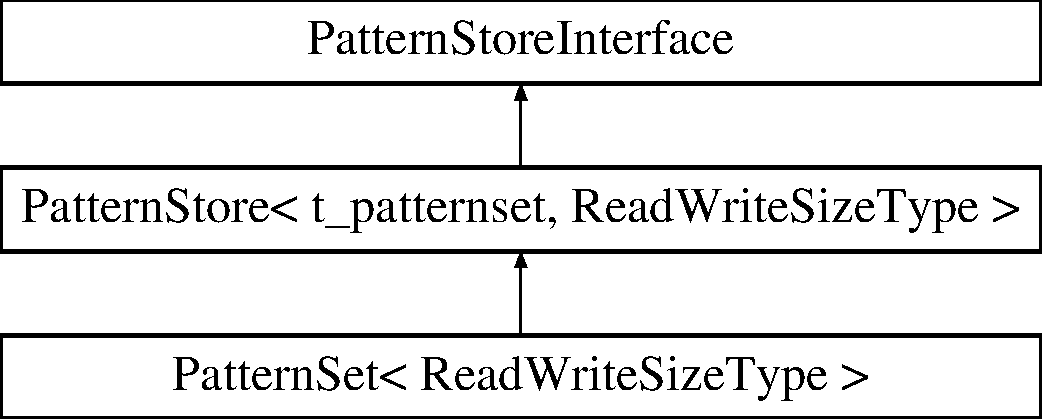
\includegraphics[height=3.000000cm]{classPatternSet}
\end{center}
\end{figure}
\subsection*{Public Types}
\begin{DoxyCompactItemize}
\item 
typedef t\+\_\+patternset\+::iterator \hyperlink{classPatternSet_a18b78ea966c57db2373741291ba610f3}{iterator}
\item 
typedef t\+\_\+patternset\+::const\+\_\+iterator \hyperlink{classPatternSet_a5d419991ea0abb0fbc4a2282574b1b8c}{const\+\_\+iterator}
\end{DoxyCompactItemize}
\subsection*{Public Member Functions}
\begin{DoxyCompactItemize}
\item 
\hyperlink{classPatternSet_a8cf2b4c7f096c7a3a7d17342c0153154}{Pattern\+Set} ()
\item 
\hyperlink{classPatternSet_a0174aa499a90c0a191fb3ad9d003c343}{Pattern\+Set} (const \hyperlink{classClassDecoder}{Class\+Decoder} \&classdecoder)
\item 
\hyperlink{classPatternSet_a693cd64ce7f5ab7f0e9c2dc15d8179fe}{Pattern\+Set} (const \hyperlink{classClassEncoder}{Class\+Encoder} \&classencoder)
\item 
virtual \hyperlink{classPatternSet_a4a521fd6ed29c03dad6e665cfe840a01}{$\sim$\+Pattern\+Set} ()
\item 
void \hyperlink{classPatternSet_aee78dae3e67875f22089ba537d50bc29}{insert} (const \hyperlink{classPattern}{Pattern} \&pattern)
\item 
bool \hyperlink{classPatternSet_a25e9ec9ca33750f21dd729cd2462d925}{has} (const \hyperlink{classPattern}{Pattern} \&pattern) const 
\item 
bool \hyperlink{classPatternSet_a28de1eeb8ec5774505173cc28e06320e}{has} (const \hyperlink{classPatternPointer}{Pattern\+Pointer} \&pattern) const 
\item 
size\+\_\+t \hyperlink{classPatternSet_af85860d7135a5154a01a8366131beb39}{size} () const 
\item 
void \hyperlink{classPatternSet_ac66abd4ac79ee7d35548a3bbfd8e5e8f}{reserve} (size\+\_\+t s)
\item 
\hyperlink{classPatternSet_a18b78ea966c57db2373741291ba610f3}{iterator} \hyperlink{classPatternSet_ac8c206e63c54d45443a38df762cea863}{begin} ()
\item 
\hyperlink{classPatternSet_a5d419991ea0abb0fbc4a2282574b1b8c}{const\+\_\+iterator} \hyperlink{classPatternSet_af78486457770e3260e73fc233b789a1a}{begin} () const 
\item 
\hyperlink{classPatternSet_a18b78ea966c57db2373741291ba610f3}{iterator} \hyperlink{classPatternSet_a8ef5ec893a3ab9b00cf70cfdf2e623b9}{end} ()
\item 
\hyperlink{classPatternSet_a5d419991ea0abb0fbc4a2282574b1b8c}{const\+\_\+iterator} \hyperlink{classPatternSet_af0b085d67c1aa4c38aa40451868a8500}{end} () const 
\item 
\hyperlink{classPatternSet_a18b78ea966c57db2373741291ba610f3}{iterator} \hyperlink{classPatternSet_a2c56aa5b266f2132f8453bf794bba1f5}{find} (const \hyperlink{classPattern}{Pattern} \&pattern)
\item 
\hyperlink{classPatternSet_a5d419991ea0abb0fbc4a2282574b1b8c}{const\+\_\+iterator} \hyperlink{classPatternSet_a56c0fcc8deb357628e778d3cc0d3c418}{find} (const \hyperlink{classPattern}{Pattern} \&pattern) const 
\item 
\hyperlink{classPatternSet_a18b78ea966c57db2373741291ba610f3}{iterator} \hyperlink{classPatternSet_a0463855da3729a70a59ee2e24265fbf8}{find} (const \hyperlink{classPatternPointer}{Pattern\+Pointer} \&pattern)
\item 
\hyperlink{classPatternSet_a5d419991ea0abb0fbc4a2282574b1b8c}{const\+\_\+iterator} \hyperlink{classPatternSet_acba3d1e3b3bce94f6768c014b0d17140}{find} (const \hyperlink{classPatternPointer}{Pattern\+Pointer} \&pattern) const 
\item 
bool \hyperlink{classPatternSet_afd2c053ac589e30edd7eda5c9f95c771}{erase} (const \hyperlink{classPattern}{Pattern} \&pattern)
\item 
\hyperlink{classPatternSet_a18b78ea966c57db2373741291ba610f3}{iterator} \hyperlink{classPatternSet_afbcbec2296a6ea98b809dcd9288eb756}{erase} (\hyperlink{classPatternSet_a5d419991ea0abb0fbc4a2282574b1b8c}{const\+\_\+iterator} position)
\item 
void \hyperlink{classPatternSet_ae55073ee2384d529faf51fca22c8dee1}{write} (std\+::ostream $\ast$out)
\item 
void \hyperlink{classPatternSet_a97bff883909c96f3f8a07a9c9ef83d84}{read} (std\+::istream $\ast$in, int M\+I\+N\+L\+E\+N\+G\+T\+H=0, int M\+A\+X\+L\+E\+N\+G\+T\+H=999999, \hyperlink{classPatternStoreInterface}{Pattern\+Store\+Interface} $\ast$constrainstore=N\+U\+L\+L, bool D\+O\+N\+G\+R\+A\+M\+S=true, bool D\+O\+S\+K\+I\+P\+G\+R\+A\+M\+S=true, bool D\+O\+F\+L\+E\+X\+G\+R\+A\+M\+S=true)
\item 
{\footnotesize template$<$class Read\+Value\+Type , class Read\+Value\+Handler  = Base\+Value\+Handler$<$\+Read\+Value\+Type$>$$>$ }\\void \hyperlink{classPatternSet_a7c974deb65a7b48ada65a4b4a45a5a3f}{readmap} (std\+::istream $\ast$in, int M\+I\+N\+T\+O\+K\+E\+N\+S=0, int M\+I\+N\+L\+E\+N\+G\+T\+H=0, int M\+A\+X\+L\+E\+N\+G\+T\+H=999999, \hyperlink{classPatternStoreInterface}{Pattern\+Store\+Interface} $\ast$constrainstore=N\+U\+L\+L, bool D\+O\+N\+G\+R\+A\+M\+S=true, bool D\+O\+S\+K\+I\+P\+G\+R\+A\+M\+S=true, bool D\+O\+F\+L\+E\+X\+G\+R\+A\+M\+S=true)
\end{DoxyCompactItemize}
\subsection*{Protected Attributes}
\begin{DoxyCompactItemize}
\item 
\hyperlink{patternstore_8h_a29bbbbc6d95519f30358276784e16c25}{t\+\_\+patternset} \hyperlink{classPatternSet_afa1d4a71d4b1f17a5fa5fba98f637687}{data}
\end{DoxyCompactItemize}


\subsection{Detailed Description}
\subsubsection*{template$<$class Read\+Write\+Size\+Type = uint32\+\_\+t$>$class Pattern\+Set$<$ Read\+Write\+Size\+Type $>$}

A pattern store in the form of an unordered set (i.\+e, no duplicates). Stores only patterns, no values. 


\begin{DoxyTemplParams}{Template Parameters}
{\em Read\+Write\+Size\+Type} & The data type for addressing, determines the maximum amount of patterns that can be held, only used in serialisation/deserialisation \\
\hline
\end{DoxyTemplParams}


\subsection{Member Typedef Documentation}
\hypertarget{classPatternSet_a5d419991ea0abb0fbc4a2282574b1b8c}{}\index{Pattern\+Set@{Pattern\+Set}!const\+\_\+iterator@{const\+\_\+iterator}}
\index{const\+\_\+iterator@{const\+\_\+iterator}!Pattern\+Set@{Pattern\+Set}}
\subsubsection[{const\+\_\+iterator}]{\setlength{\rightskip}{0pt plus 5cm}template$<$class Read\+Write\+Size\+Type = uint32\+\_\+t$>$ typedef t\+\_\+patternset\+::const\+\_\+iterator {\bf Pattern\+Set}$<$ Read\+Write\+Size\+Type $>$\+::{\bf const\+\_\+iterator}}\label{classPatternSet_a5d419991ea0abb0fbc4a2282574b1b8c}
\hypertarget{classPatternSet_a18b78ea966c57db2373741291ba610f3}{}\index{Pattern\+Set@{Pattern\+Set}!iterator@{iterator}}
\index{iterator@{iterator}!Pattern\+Set@{Pattern\+Set}}
\subsubsection[{iterator}]{\setlength{\rightskip}{0pt plus 5cm}template$<$class Read\+Write\+Size\+Type = uint32\+\_\+t$>$ typedef t\+\_\+patternset\+::iterator {\bf Pattern\+Set}$<$ Read\+Write\+Size\+Type $>$\+::{\bf iterator}}\label{classPatternSet_a18b78ea966c57db2373741291ba610f3}


\subsection{Constructor \& Destructor Documentation}
\hypertarget{classPatternSet_a8cf2b4c7f096c7a3a7d17342c0153154}{}\index{Pattern\+Set@{Pattern\+Set}!Pattern\+Set@{Pattern\+Set}}
\index{Pattern\+Set@{Pattern\+Set}!Pattern\+Set@{Pattern\+Set}}
\subsubsection[{Pattern\+Set()}]{\setlength{\rightskip}{0pt plus 5cm}template$<$class Read\+Write\+Size\+Type = uint32\+\_\+t$>$ {\bf Pattern\+Set}$<$ Read\+Write\+Size\+Type $>$\+::{\bf Pattern\+Set} (
\begin{DoxyParamCaption}
{}
\end{DoxyParamCaption}
)\hspace{0.3cm}{\ttfamily [inline]}}\label{classPatternSet_a8cf2b4c7f096c7a3a7d17342c0153154}
Empty set constructor \hypertarget{classPatternSet_a0174aa499a90c0a191fb3ad9d003c343}{}\index{Pattern\+Set@{Pattern\+Set}!Pattern\+Set@{Pattern\+Set}}
\index{Pattern\+Set@{Pattern\+Set}!Pattern\+Set@{Pattern\+Set}}
\subsubsection[{Pattern\+Set(const Class\+Decoder \&classdecoder)}]{\setlength{\rightskip}{0pt plus 5cm}template$<$class Read\+Write\+Size\+Type = uint32\+\_\+t$>$ {\bf Pattern\+Set}$<$ Read\+Write\+Size\+Type $>$\+::{\bf Pattern\+Set} (
\begin{DoxyParamCaption}
\item[{const {\bf Class\+Decoder} \&}]{classdecoder}
\end{DoxyParamCaption}
)\hspace{0.3cm}{\ttfamily [inline]}}\label{classPatternSet_a0174aa499a90c0a191fb3ad9d003c343}
Constructs a pattern set from a \hyperlink{classClassDecoder}{Class\+Decoder} \hypertarget{classPatternSet_a693cd64ce7f5ab7f0e9c2dc15d8179fe}{}\index{Pattern\+Set@{Pattern\+Set}!Pattern\+Set@{Pattern\+Set}}
\index{Pattern\+Set@{Pattern\+Set}!Pattern\+Set@{Pattern\+Set}}
\subsubsection[{Pattern\+Set(const Class\+Encoder \&classencoder)}]{\setlength{\rightskip}{0pt plus 5cm}template$<$class Read\+Write\+Size\+Type = uint32\+\_\+t$>$ {\bf Pattern\+Set}$<$ Read\+Write\+Size\+Type $>$\+::{\bf Pattern\+Set} (
\begin{DoxyParamCaption}
\item[{const {\bf Class\+Encoder} \&}]{classencoder}
\end{DoxyParamCaption}
)\hspace{0.3cm}{\ttfamily [inline]}}\label{classPatternSet_a693cd64ce7f5ab7f0e9c2dc15d8179fe}
Constructs a pattern set from a \hyperlink{classClassEncoder}{Class\+Encoder} \hypertarget{classPatternSet_a4a521fd6ed29c03dad6e665cfe840a01}{}\index{Pattern\+Set@{Pattern\+Set}!````~Pattern\+Set@{$\sim$\+Pattern\+Set}}
\index{````~Pattern\+Set@{$\sim$\+Pattern\+Set}!Pattern\+Set@{Pattern\+Set}}
\subsubsection[{$\sim$\+Pattern\+Set()}]{\setlength{\rightskip}{0pt plus 5cm}template$<$class Read\+Write\+Size\+Type = uint32\+\_\+t$>$ virtual {\bf Pattern\+Set}$<$ Read\+Write\+Size\+Type $>$\+::$\sim${\bf Pattern\+Set} (
\begin{DoxyParamCaption}
{}
\end{DoxyParamCaption}
)\hspace{0.3cm}{\ttfamily [inline]}, {\ttfamily [virtual]}}\label{classPatternSet_a4a521fd6ed29c03dad6e665cfe840a01}


\subsection{Member Function Documentation}
\hypertarget{classPatternSet_ac8c206e63c54d45443a38df762cea863}{}\index{Pattern\+Set@{Pattern\+Set}!begin@{begin}}
\index{begin@{begin}!Pattern\+Set@{Pattern\+Set}}
\subsubsection[{begin()}]{\setlength{\rightskip}{0pt plus 5cm}template$<$class Read\+Write\+Size\+Type = uint32\+\_\+t$>$ {\bf iterator} {\bf Pattern\+Set}$<$ Read\+Write\+Size\+Type $>$\+::begin (
\begin{DoxyParamCaption}
{}
\end{DoxyParamCaption}
)\hspace{0.3cm}{\ttfamily [inline]}, {\ttfamily [virtual]}}\label{classPatternSet_ac8c206e63c54d45443a38df762cea863}
Returns an iterator to iterate over the set 

Implements \hyperlink{classPatternStore_aab3fab217b585b2b90a3fb3cc7065e11}{Pattern\+Store$<$ t\+\_\+patternset, Read\+Write\+Size\+Type, Pattern $>$}.

\hypertarget{classPatternSet_af78486457770e3260e73fc233b789a1a}{}\index{Pattern\+Set@{Pattern\+Set}!begin@{begin}}
\index{begin@{begin}!Pattern\+Set@{Pattern\+Set}}
\subsubsection[{begin() const }]{\setlength{\rightskip}{0pt plus 5cm}template$<$class Read\+Write\+Size\+Type = uint32\+\_\+t$>$ {\bf const\+\_\+iterator} {\bf Pattern\+Set}$<$ Read\+Write\+Size\+Type $>$\+::begin (
\begin{DoxyParamCaption}
{}
\end{DoxyParamCaption}
) const\hspace{0.3cm}{\ttfamily [inline]}}\label{classPatternSet_af78486457770e3260e73fc233b789a1a}
\hypertarget{classPatternSet_a8ef5ec893a3ab9b00cf70cfdf2e623b9}{}\index{Pattern\+Set@{Pattern\+Set}!end@{end}}
\index{end@{end}!Pattern\+Set@{Pattern\+Set}}
\subsubsection[{end()}]{\setlength{\rightskip}{0pt plus 5cm}template$<$class Read\+Write\+Size\+Type = uint32\+\_\+t$>$ {\bf iterator} {\bf Pattern\+Set}$<$ Read\+Write\+Size\+Type $>$\+::end (
\begin{DoxyParamCaption}
{}
\end{DoxyParamCaption}
)\hspace{0.3cm}{\ttfamily [inline]}, {\ttfamily [virtual]}}\label{classPatternSet_a8ef5ec893a3ab9b00cf70cfdf2e623b9}


Implements \hyperlink{classPatternStore_ae697b6ba815e09fa300532a78e1c9077}{Pattern\+Store$<$ t\+\_\+patternset, Read\+Write\+Size\+Type, Pattern $>$}.

\hypertarget{classPatternSet_af0b085d67c1aa4c38aa40451868a8500}{}\index{Pattern\+Set@{Pattern\+Set}!end@{end}}
\index{end@{end}!Pattern\+Set@{Pattern\+Set}}
\subsubsection[{end() const }]{\setlength{\rightskip}{0pt plus 5cm}template$<$class Read\+Write\+Size\+Type = uint32\+\_\+t$>$ {\bf const\+\_\+iterator} {\bf Pattern\+Set}$<$ Read\+Write\+Size\+Type $>$\+::end (
\begin{DoxyParamCaption}
{}
\end{DoxyParamCaption}
) const\hspace{0.3cm}{\ttfamily [inline]}}\label{classPatternSet_af0b085d67c1aa4c38aa40451868a8500}
\hypertarget{classPatternSet_afd2c053ac589e30edd7eda5c9f95c771}{}\index{Pattern\+Set@{Pattern\+Set}!erase@{erase}}
\index{erase@{erase}!Pattern\+Set@{Pattern\+Set}}
\subsubsection[{erase(const Pattern \&pattern)}]{\setlength{\rightskip}{0pt plus 5cm}template$<$class Read\+Write\+Size\+Type = uint32\+\_\+t$>$ bool {\bf Pattern\+Set}$<$ Read\+Write\+Size\+Type $>$\+::erase (
\begin{DoxyParamCaption}
\item[{const {\bf Pattern} \&}]{pattern}
\end{DoxyParamCaption}
)\hspace{0.3cm}{\ttfamily [inline]}, {\ttfamily [virtual]}}\label{classPatternSet_afd2c053ac589e30edd7eda5c9f95c771}
Removes the specified pattern from the set, returns true if successful 

Implements \hyperlink{classPatternStore_a42f8de80a8627c485315e4bb8eff538f}{Pattern\+Store$<$ t\+\_\+patternset, Read\+Write\+Size\+Type, Pattern $>$}.

\hypertarget{classPatternSet_afbcbec2296a6ea98b809dcd9288eb756}{}\index{Pattern\+Set@{Pattern\+Set}!erase@{erase}}
\index{erase@{erase}!Pattern\+Set@{Pattern\+Set}}
\subsubsection[{erase(const\+\_\+iterator position)}]{\setlength{\rightskip}{0pt plus 5cm}template$<$class Read\+Write\+Size\+Type = uint32\+\_\+t$>$ {\bf iterator} {\bf Pattern\+Set}$<$ Read\+Write\+Size\+Type $>$\+::erase (
\begin{DoxyParamCaption}
\item[{{\bf const\+\_\+iterator}}]{position}
\end{DoxyParamCaption}
)\hspace{0.3cm}{\ttfamily [inline]}}\label{classPatternSet_afbcbec2296a6ea98b809dcd9288eb756}
\hypertarget{classPatternSet_a2c56aa5b266f2132f8453bf794bba1f5}{}\index{Pattern\+Set@{Pattern\+Set}!find@{find}}
\index{find@{find}!Pattern\+Set@{Pattern\+Set}}
\subsubsection[{find(const Pattern \&pattern)}]{\setlength{\rightskip}{0pt plus 5cm}template$<$class Read\+Write\+Size\+Type = uint32\+\_\+t$>$ {\bf iterator} {\bf Pattern\+Set}$<$ Read\+Write\+Size\+Type $>$\+::find (
\begin{DoxyParamCaption}
\item[{const {\bf Pattern} \&}]{pattern}
\end{DoxyParamCaption}
)\hspace{0.3cm}{\ttfamily [inline]}, {\ttfamily [virtual]}}\label{classPatternSet_a2c56aa5b266f2132f8453bf794bba1f5}
Returns an iterator to the pattern in the set or \hyperlink{classPatternSet_a8ef5ec893a3ab9b00cf70cfdf2e623b9}{end()} if no such pattern was found. 

Implements \hyperlink{classPatternStore_a6996798c63c2dd3ae3845848da35a6dd}{Pattern\+Store$<$ t\+\_\+patternset, Read\+Write\+Size\+Type, Pattern $>$}.

\hypertarget{classPatternSet_a56c0fcc8deb357628e778d3cc0d3c418}{}\index{Pattern\+Set@{Pattern\+Set}!find@{find}}
\index{find@{find}!Pattern\+Set@{Pattern\+Set}}
\subsubsection[{find(const Pattern \&pattern) const }]{\setlength{\rightskip}{0pt plus 5cm}template$<$class Read\+Write\+Size\+Type = uint32\+\_\+t$>$ {\bf const\+\_\+iterator} {\bf Pattern\+Set}$<$ Read\+Write\+Size\+Type $>$\+::find (
\begin{DoxyParamCaption}
\item[{const {\bf Pattern} \&}]{pattern}
\end{DoxyParamCaption}
) const\hspace{0.3cm}{\ttfamily [inline]}}\label{classPatternSet_a56c0fcc8deb357628e778d3cc0d3c418}
\hypertarget{classPatternSet_a0463855da3729a70a59ee2e24265fbf8}{}\index{Pattern\+Set@{Pattern\+Set}!find@{find}}
\index{find@{find}!Pattern\+Set@{Pattern\+Set}}
\subsubsection[{find(const Pattern\+Pointer \&pattern)}]{\setlength{\rightskip}{0pt plus 5cm}template$<$class Read\+Write\+Size\+Type = uint32\+\_\+t$>$ {\bf iterator} {\bf Pattern\+Set}$<$ Read\+Write\+Size\+Type $>$\+::find (
\begin{DoxyParamCaption}
\item[{const {\bf Pattern\+Pointer} \&}]{pattern}
\end{DoxyParamCaption}
)\hspace{0.3cm}{\ttfamily [inline]}, {\ttfamily [virtual]}}\label{classPatternSet_a0463855da3729a70a59ee2e24265fbf8}


Implements \hyperlink{classPatternStore_a33991d30a74b13a4264200474bf0542c}{Pattern\+Store$<$ t\+\_\+patternset, Read\+Write\+Size\+Type, Pattern $>$}.

\hypertarget{classPatternSet_acba3d1e3b3bce94f6768c014b0d17140}{}\index{Pattern\+Set@{Pattern\+Set}!find@{find}}
\index{find@{find}!Pattern\+Set@{Pattern\+Set}}
\subsubsection[{find(const Pattern\+Pointer \&pattern) const }]{\setlength{\rightskip}{0pt plus 5cm}template$<$class Read\+Write\+Size\+Type = uint32\+\_\+t$>$ {\bf const\+\_\+iterator} {\bf Pattern\+Set}$<$ Read\+Write\+Size\+Type $>$\+::find (
\begin{DoxyParamCaption}
\item[{const {\bf Pattern\+Pointer} \&}]{pattern}
\end{DoxyParamCaption}
) const\hspace{0.3cm}{\ttfamily [inline]}}\label{classPatternSet_acba3d1e3b3bce94f6768c014b0d17140}
\hypertarget{classPatternSet_a25e9ec9ca33750f21dd729cd2462d925}{}\index{Pattern\+Set@{Pattern\+Set}!has@{has}}
\index{has@{has}!Pattern\+Set@{Pattern\+Set}}
\subsubsection[{has(const Pattern \&pattern) const }]{\setlength{\rightskip}{0pt plus 5cm}template$<$class Read\+Write\+Size\+Type = uint32\+\_\+t$>$ bool {\bf Pattern\+Set}$<$ Read\+Write\+Size\+Type $>$\+::has (
\begin{DoxyParamCaption}
\item[{const {\bf Pattern} \&}]{pattern}
\end{DoxyParamCaption}
) const\hspace{0.3cm}{\ttfamily [inline]}, {\ttfamily [virtual]}}\label{classPatternSet_a25e9ec9ca33750f21dd729cd2462d925}
Checks if a pattern is in the set 

Implements \hyperlink{classPatternStore_a2e29add9b35b3459d183f56f6c5525ed}{Pattern\+Store$<$ t\+\_\+patternset, Read\+Write\+Size\+Type, Pattern $>$}.

\hypertarget{classPatternSet_a28de1eeb8ec5774505173cc28e06320e}{}\index{Pattern\+Set@{Pattern\+Set}!has@{has}}
\index{has@{has}!Pattern\+Set@{Pattern\+Set}}
\subsubsection[{has(const Pattern\+Pointer \&pattern) const }]{\setlength{\rightskip}{0pt plus 5cm}template$<$class Read\+Write\+Size\+Type = uint32\+\_\+t$>$ bool {\bf Pattern\+Set}$<$ Read\+Write\+Size\+Type $>$\+::has (
\begin{DoxyParamCaption}
\item[{const {\bf Pattern\+Pointer} \&}]{pattern}
\end{DoxyParamCaption}
) const\hspace{0.3cm}{\ttfamily [inline]}, {\ttfamily [virtual]}}\label{classPatternSet_a28de1eeb8ec5774505173cc28e06320e}
Checks if a pattern is in the set 

Implements \hyperlink{classPatternStore_ad1e06c2468bad2a14d4ed28b26c6ff33}{Pattern\+Store$<$ t\+\_\+patternset, Read\+Write\+Size\+Type, Pattern $>$}.

\hypertarget{classPatternSet_aee78dae3e67875f22089ba537d50bc29}{}\index{Pattern\+Set@{Pattern\+Set}!insert@{insert}}
\index{insert@{insert}!Pattern\+Set@{Pattern\+Set}}
\subsubsection[{insert(const Pattern \&pattern)}]{\setlength{\rightskip}{0pt plus 5cm}template$<$class Read\+Write\+Size\+Type = uint32\+\_\+t$>$ void {\bf Pattern\+Set}$<$ Read\+Write\+Size\+Type $>$\+::insert (
\begin{DoxyParamCaption}
\item[{const {\bf Pattern} \&}]{pattern}
\end{DoxyParamCaption}
)\hspace{0.3cm}{\ttfamily [inline]}, {\ttfamily [virtual]}}\label{classPatternSet_aee78dae3e67875f22089ba537d50bc29}
Add a new pattern to the set 

Implements \hyperlink{classPatternStore_aac1558cd3f7e4ec8ec142e1c59f122c9}{Pattern\+Store$<$ t\+\_\+patternset, Read\+Write\+Size\+Type, Pattern $>$}.

\hypertarget{classPatternSet_a97bff883909c96f3f8a07a9c9ef83d84}{}\index{Pattern\+Set@{Pattern\+Set}!read@{read}}
\index{read@{read}!Pattern\+Set@{Pattern\+Set}}
\subsubsection[{read(std\+::istream $\ast$in, int M\+I\+N\+L\+E\+N\+G\+T\+H=0, int M\+A\+X\+L\+E\+N\+G\+T\+H=999999, Pattern\+Store\+Interface $\ast$constrainstore=\+N\+U\+L\+L, bool D\+O\+N\+G\+R\+A\+M\+S=true, bool D\+O\+S\+K\+I\+P\+G\+R\+A\+M\+S=true, bool D\+O\+F\+L\+E\+X\+G\+R\+A\+M\+S=true)}]{\setlength{\rightskip}{0pt plus 5cm}template$<$class Read\+Write\+Size\+Type = uint32\+\_\+t$>$ void {\bf Pattern\+Set}$<$ Read\+Write\+Size\+Type $>$\+::read (
\begin{DoxyParamCaption}
\item[{std\+::istream $\ast$}]{in, }
\item[{int}]{M\+I\+N\+L\+E\+N\+G\+T\+H = {\ttfamily 0}, }
\item[{int}]{M\+A\+X\+L\+E\+N\+G\+T\+H = {\ttfamily 999999}, }
\item[{{\bf Pattern\+Store\+Interface} $\ast$}]{constrainstore = {\ttfamily NULL}, }
\item[{bool}]{D\+O\+N\+G\+R\+A\+M\+S = {\ttfamily true}, }
\item[{bool}]{D\+O\+S\+K\+I\+P\+G\+R\+A\+M\+S = {\ttfamily true}, }
\item[{bool}]{D\+O\+F\+L\+E\+X\+G\+R\+A\+M\+S = {\ttfamily true}}
\end{DoxyParamCaption}
)\hspace{0.3cm}{\ttfamily [inline]}}\label{classPatternSet_a97bff883909c96f3f8a07a9c9ef83d84}
Read the set from input stream, in binary format \hypertarget{classPatternSet_a7c974deb65a7b48ada65a4b4a45a5a3f}{}\index{Pattern\+Set@{Pattern\+Set}!readmap@{readmap}}
\index{readmap@{readmap}!Pattern\+Set@{Pattern\+Set}}
\subsubsection[{readmap(std\+::istream $\ast$in, int M\+I\+N\+T\+O\+K\+E\+N\+S=0, int M\+I\+N\+L\+E\+N\+G\+T\+H=0, int M\+A\+X\+L\+E\+N\+G\+T\+H=999999, Pattern\+Store\+Interface $\ast$constrainstore=\+N\+U\+L\+L, bool D\+O\+N\+G\+R\+A\+M\+S=true, bool D\+O\+S\+K\+I\+P\+G\+R\+A\+M\+S=true, bool D\+O\+F\+L\+E\+X\+G\+R\+A\+M\+S=true)}]{\setlength{\rightskip}{0pt plus 5cm}template$<$class Read\+Write\+Size\+Type = uint32\+\_\+t$>$ template$<$class Read\+Value\+Type , class Read\+Value\+Handler  = Base\+Value\+Handler$<$\+Read\+Value\+Type$>$$>$ void {\bf Pattern\+Set}$<$ Read\+Write\+Size\+Type $>$\+::readmap (
\begin{DoxyParamCaption}
\item[{std\+::istream $\ast$}]{in, }
\item[{int}]{M\+I\+N\+T\+O\+K\+E\+N\+S = {\ttfamily 0}, }
\item[{int}]{M\+I\+N\+L\+E\+N\+G\+T\+H = {\ttfamily 0}, }
\item[{int}]{M\+A\+X\+L\+E\+N\+G\+T\+H = {\ttfamily 999999}, }
\item[{{\bf Pattern\+Store\+Interface} $\ast$}]{constrainstore = {\ttfamily NULL}, }
\item[{bool}]{D\+O\+N\+G\+R\+A\+M\+S = {\ttfamily true}, }
\item[{bool}]{D\+O\+S\+K\+I\+P\+G\+R\+A\+M\+S = {\ttfamily true}, }
\item[{bool}]{D\+O\+F\+L\+E\+X\+G\+R\+A\+M\+S = {\ttfamily true}}
\end{DoxyParamCaption}
)\hspace{0.3cm}{\ttfamily [inline]}}\label{classPatternSet_a7c974deb65a7b48ada65a4b4a45a5a3f}
Reads a map from input stream, in binary format, but ignores the values and retains only the keys for the set. \hypertarget{classPatternSet_ac66abd4ac79ee7d35548a3bbfd8e5e8f}{}\index{Pattern\+Set@{Pattern\+Set}!reserve@{reserve}}
\index{reserve@{reserve}!Pattern\+Set@{Pattern\+Set}}
\subsubsection[{reserve(size\+\_\+t s)}]{\setlength{\rightskip}{0pt plus 5cm}template$<$class Read\+Write\+Size\+Type = uint32\+\_\+t$>$ void {\bf Pattern\+Set}$<$ Read\+Write\+Size\+Type $>$\+::reserve (
\begin{DoxyParamCaption}
\item[{size\+\_\+t}]{s}
\end{DoxyParamCaption}
)\hspace{0.3cm}{\ttfamily [inline]}, {\ttfamily [virtual]}}\label{classPatternSet_ac66abd4ac79ee7d35548a3bbfd8e5e8f}


Implements \hyperlink{classPatternStore_afc995f7b88b6a31b700bb3bdb948b180}{Pattern\+Store$<$ t\+\_\+patternset, Read\+Write\+Size\+Type, Pattern $>$}.

\hypertarget{classPatternSet_af85860d7135a5154a01a8366131beb39}{}\index{Pattern\+Set@{Pattern\+Set}!size@{size}}
\index{size@{size}!Pattern\+Set@{Pattern\+Set}}
\subsubsection[{size() const }]{\setlength{\rightskip}{0pt plus 5cm}template$<$class Read\+Write\+Size\+Type = uint32\+\_\+t$>$ size\+\_\+t {\bf Pattern\+Set}$<$ Read\+Write\+Size\+Type $>$\+::size (
\begin{DoxyParamCaption}
{}
\end{DoxyParamCaption}
) const\hspace{0.3cm}{\ttfamily [inline]}, {\ttfamily [virtual]}}\label{classPatternSet_af85860d7135a5154a01a8366131beb39}
Returns the number of patterns in the set 

Implements \hyperlink{classPatternStore_abfa82df94ab565bea13fc45ee4866faf}{Pattern\+Store$<$ t\+\_\+patternset, Read\+Write\+Size\+Type, Pattern $>$}.

\hypertarget{classPatternSet_ae55073ee2384d529faf51fca22c8dee1}{}\index{Pattern\+Set@{Pattern\+Set}!write@{write}}
\index{write@{write}!Pattern\+Set@{Pattern\+Set}}
\subsubsection[{write(std\+::ostream $\ast$out)}]{\setlength{\rightskip}{0pt plus 5cm}template$<$class Read\+Write\+Size\+Type = uint32\+\_\+t$>$ void {\bf Pattern\+Set}$<$ Read\+Write\+Size\+Type $>$\+::write (
\begin{DoxyParamCaption}
\item[{std\+::ostream $\ast$}]{out}
\end{DoxyParamCaption}
)\hspace{0.3cm}{\ttfamily [inline]}, {\ttfamily [virtual]}}\label{classPatternSet_ae55073ee2384d529faf51fca22c8dee1}
Write the set to output stream, in binary format 

Implements \hyperlink{classPatternStore_a70d9b8faa5858ab7182cea7b1488a75c}{Pattern\+Store$<$ t\+\_\+patternset, Read\+Write\+Size\+Type, Pattern $>$}.



\subsection{Member Data Documentation}
\hypertarget{classPatternSet_afa1d4a71d4b1f17a5fa5fba98f637687}{}\index{Pattern\+Set@{Pattern\+Set}!data@{data}}
\index{data@{data}!Pattern\+Set@{Pattern\+Set}}
\subsubsection[{data}]{\setlength{\rightskip}{0pt plus 5cm}template$<$class Read\+Write\+Size\+Type = uint32\+\_\+t$>$ {\bf t\+\_\+patternset} {\bf Pattern\+Set}$<$ Read\+Write\+Size\+Type $>$\+::data\hspace{0.3cm}{\ttfamily [protected]}}\label{classPatternSet_afa1d4a71d4b1f17a5fa5fba98f637687}


The documentation for this class was generated from the following file\+:\begin{DoxyCompactItemize}
\item 
include/\hyperlink{patternstore_8h}{patternstore.\+h}\end{DoxyCompactItemize}

\hypertarget{classPatternSetModel}{}\section{Pattern\+Set\+Model Class Reference}
\label{classPatternSetModel}\index{Pattern\+Set\+Model@{Pattern\+Set\+Model}}


A pattern model based on an unordered set, does not hold data, only patterns. Very suitable for loading constraint models.  




{\ttfamily \#include $<$patternmodel.\+h$>$}

Inheritance diagram for Pattern\+Set\+Model\+:\begin{figure}[H]
\begin{center}
\leavevmode
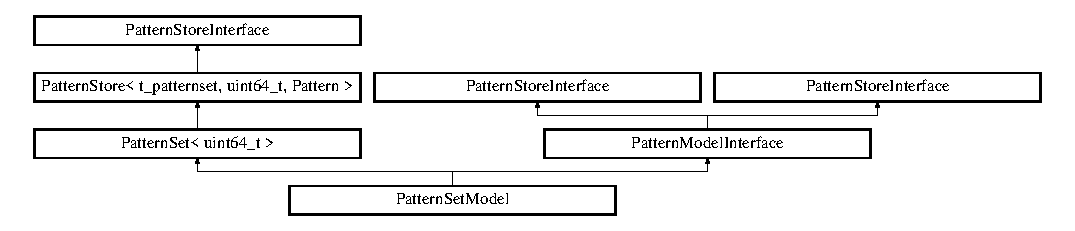
\includegraphics[height=2.657177cm]{classPatternSetModel}
\end{center}
\end{figure}
\subsection*{Public Types}
\begin{DoxyCompactItemize}
\item 
typedef \hyperlink{classPatternSet}{Pattern\+Set}$<$ uint64\+\_\+t $>$\+::\hyperlink{classPatternSetModel_a59468751dd558f75f6ddaa514b93ff07}{iterator} \hyperlink{classPatternSetModel_a59468751dd558f75f6ddaa514b93ff07}{iterator}
\item 
typedef \hyperlink{classPatternSet}{Pattern\+Set}$<$ uint64\+\_\+t $>$\+::\hyperlink{classPatternSetModel_aca006659665c67916ea64d89b16a46e4}{const\+\_\+iterator} \hyperlink{classPatternSetModel_aca006659665c67916ea64d89b16a46e4}{const\+\_\+iterator}
\end{DoxyCompactItemize}
\subsection*{Public Member Functions}
\begin{DoxyCompactItemize}
\item 
\hyperlink{classPatternSetModel_a983877848beaf832f41f747231e1bf6f}{Pattern\+Set\+Model} ()
\item 
\hyperlink{classPatternSetModel_aecf0741defc687aff8e69514742c697d}{Pattern\+Set\+Model} (std\+::istream $\ast$f, \hyperlink{classPatternModelOptions}{Pattern\+Model\+Options} options, \hyperlink{classPatternModelInterface}{Pattern\+Model\+Interface} $\ast$constrainmodel=N\+U\+L\+L)
\item 
\hyperlink{classPatternSetModel_a31c7d5c3e0165fa832d8fc85f292bd1e}{Pattern\+Set\+Model} (const std\+::string \&filename, const \hyperlink{classPatternModelOptions}{Pattern\+Model\+Options} \&options, \hyperlink{classPatternModelInterface}{Pattern\+Model\+Interface} $\ast$constrainmodel=N\+U\+L\+L)
\item 
virtual int \hyperlink{classPatternSetModel_a27adf3033f15f03e908d53d032779d09}{getmodeltype} () const 
\item 
virtual int \hyperlink{classPatternSetModel_a79dc7fd04e3de5eb894541bd664f5d12}{getmodelversion} () const 
\item 
virtual size\+\_\+t \hyperlink{classPatternSetModel_aa19ae308dbc4bf1db35be6ba7ff4769b}{size} () const 
\item 
virtual bool \hyperlink{classPatternSetModel_a8821cf7c6d469d0978e32e5ed9cfcda0}{has} (const \hyperlink{classPattern}{Pattern} \&pattern) const 
\item 
virtual bool \hyperlink{classPatternSetModel_a2fcd4d3d1023b5e20f67d2b845a29b2f}{has} (const \hyperlink{classPatternPointer}{Pattern\+Pointer} \&pattern) const 
\item 
virtual void \hyperlink{classPatternSetModel_af6c3d508fd01352eeb3ae90c438db24b}{load} (std\+::string \&filename, const \hyperlink{classPatternModelOptions}{Pattern\+Model\+Options} \&options, \hyperlink{classPatternModelInterface}{Pattern\+Model\+Interface} $\ast$constrainmodel=N\+U\+L\+L)
\item 
virtual void \hyperlink{classPatternSetModel_a61c9e25adefa734946a7571a0444049f}{load} (std\+::istream $\ast$f, const \hyperlink{classPatternModelOptions}{Pattern\+Model\+Options} \&options, \hyperlink{classPatternModelInterface}{Pattern\+Model\+Interface} $\ast$constrainmodel=N\+U\+L\+L)
\item 
void \hyperlink{classPatternSetModel_a8b5731f823fd868cfc6b219e01b13343}{write} (std\+::ostream $\ast$out)
\item 
void \hyperlink{classPatternSetModel_a9ad4bb51ec6c1272b4d73168e8267c2c}{write} (const std\+::string \&filename)
\item 
\hyperlink{classPatternModelInterface}{Pattern\+Model\+Interface} $\ast$ \hyperlink{classPatternSetModel_af2ead0d1766424cb00e95f76cab0c334}{getinterface} ()
\item 
virtual unsigned int \hyperlink{classPatternSetModel_ab1ca42eb82df349263b10c57f968678e}{occurrencecount} (const \hyperlink{classPattern}{Pattern} \&pattern)
\item 
virtual double \hyperlink{classPatternSetModel_af5bdb2a283c048233e62b2a0741b7cab}{frequency} (const \hyperlink{classPattern}{Pattern} \&)
\item 
virtual int \hyperlink{classPatternSetModel_abd386cc901e2328079a349eae42d9ee8}{maxlength} () const 
\item 
virtual int \hyperlink{classPatternSetModel_a3cc6ca22d4dd68270068d5a4e05f530a}{minlength} () const 
\item 
virtual unsigned int \hyperlink{classPatternSetModel_a178d3c988a43130b4ba3d4fa57001055}{types} ()
\item 
virtual unsigned int \hyperlink{classPatternSetModel_aa834dd6a5467ea8a68680512d6251e16}{tokens} () const 
\item 
unsigned char \hyperlink{classPatternSetModel_a5ca48d3e5c9d52b3eae858d033706bf6}{type} () const 
\item 
unsigned char \hyperlink{classPatternSetModel_a664147d04aad980c5cefbffca9bb4285}{version} () const 
\end{DoxyCompactItemize}
\subsection*{Protected Attributes}
\begin{DoxyCompactItemize}
\item 
unsigned char \hyperlink{classPatternSetModel_a932b792d6f1dc488c772efb6c8530b85}{model\+\_\+type}
\item 
unsigned char \hyperlink{classPatternSetModel_ad80b50a1066615f9b20e791dfee50296}{model\+\_\+version}
\item 
uint64\+\_\+t \hyperlink{classPatternSetModel_ae64f1edc5d72066d8cc6fbb80422518b}{totaltokens}
\item 
uint64\+\_\+t \hyperlink{classPatternSetModel_ac7aeed2a7d78ef5883ba38618a3e49a7}{totaltypes}
\item 
int \hyperlink{classPatternSetModel_aa1b03b92de5af1cf36545dfbff5b56f4}{maxn}
\item 
int \hyperlink{classPatternSetModel_a52940caa8c4bb3900f75ead2cb8a97c8}{minn}
\end{DoxyCompactItemize}


\subsection{Detailed Description}
A pattern model based on an unordered set, does not hold data, only patterns. Very suitable for loading constraint models. 

\subsection{Member Typedef Documentation}
\hypertarget{classPatternSetModel_aca006659665c67916ea64d89b16a46e4}{}\index{Pattern\+Set\+Model@{Pattern\+Set\+Model}!const\+\_\+iterator@{const\+\_\+iterator}}
\index{const\+\_\+iterator@{const\+\_\+iterator}!Pattern\+Set\+Model@{Pattern\+Set\+Model}}
\subsubsection[{const\+\_\+iterator}]{\setlength{\rightskip}{0pt plus 5cm}typedef {\bf Pattern\+Set}$<$uint64\+\_\+t$>$\+::{\bf const\+\_\+iterator} {\bf Pattern\+Set\+Model\+::const\+\_\+iterator}}\label{classPatternSetModel_aca006659665c67916ea64d89b16a46e4}
\hypertarget{classPatternSetModel_a59468751dd558f75f6ddaa514b93ff07}{}\index{Pattern\+Set\+Model@{Pattern\+Set\+Model}!iterator@{iterator}}
\index{iterator@{iterator}!Pattern\+Set\+Model@{Pattern\+Set\+Model}}
\subsubsection[{iterator}]{\setlength{\rightskip}{0pt plus 5cm}typedef {\bf Pattern\+Set}$<$uint64\+\_\+t$>$\+::{\bf iterator} {\bf Pattern\+Set\+Model\+::iterator}}\label{classPatternSetModel_a59468751dd558f75f6ddaa514b93ff07}


\subsection{Constructor \& Destructor Documentation}
\hypertarget{classPatternSetModel_a983877848beaf832f41f747231e1bf6f}{}\index{Pattern\+Set\+Model@{Pattern\+Set\+Model}!Pattern\+Set\+Model@{Pattern\+Set\+Model}}
\index{Pattern\+Set\+Model@{Pattern\+Set\+Model}!Pattern\+Set\+Model@{Pattern\+Set\+Model}}
\subsubsection[{Pattern\+Set\+Model()}]{\setlength{\rightskip}{0pt plus 5cm}Pattern\+Set\+Model\+::\+Pattern\+Set\+Model (
\begin{DoxyParamCaption}
{}
\end{DoxyParamCaption}
)\hspace{0.3cm}{\ttfamily [inline]}}\label{classPatternSetModel_a983877848beaf832f41f747231e1bf6f}
Empty constructor \hypertarget{classPatternSetModel_aecf0741defc687aff8e69514742c697d}{}\index{Pattern\+Set\+Model@{Pattern\+Set\+Model}!Pattern\+Set\+Model@{Pattern\+Set\+Model}}
\index{Pattern\+Set\+Model@{Pattern\+Set\+Model}!Pattern\+Set\+Model@{Pattern\+Set\+Model}}
\subsubsection[{Pattern\+Set\+Model(std\+::istream $\ast$f, Pattern\+Model\+Options options, Pattern\+Model\+Interface $\ast$constrainmodel=\+N\+U\+L\+L)}]{\setlength{\rightskip}{0pt plus 5cm}Pattern\+Set\+Model\+::\+Pattern\+Set\+Model (
\begin{DoxyParamCaption}
\item[{std\+::istream $\ast$}]{f, }
\item[{{\bf Pattern\+Model\+Options}}]{options, }
\item[{{\bf Pattern\+Model\+Interface} $\ast$}]{constrainmodel = {\ttfamily NULL}}
\end{DoxyParamCaption}
)\hspace{0.3cm}{\ttfamily [inline]}}\label{classPatternSetModel_aecf0741defc687aff8e69514742c697d}
Load a \hyperlink{classPatternSetModel}{Pattern\+Set\+Model} from stream 
\begin{DoxyParams}{Parameters}
{\em options} & The options for loading \\
\hline
{\em constrainmodel} & Load only patterns that occur in this model \\
\hline
\end{DoxyParams}
\hypertarget{classPatternSetModel_a31c7d5c3e0165fa832d8fc85f292bd1e}{}\index{Pattern\+Set\+Model@{Pattern\+Set\+Model}!Pattern\+Set\+Model@{Pattern\+Set\+Model}}
\index{Pattern\+Set\+Model@{Pattern\+Set\+Model}!Pattern\+Set\+Model@{Pattern\+Set\+Model}}
\subsubsection[{Pattern\+Set\+Model(const std\+::string \&filename, const Pattern\+Model\+Options \&options, Pattern\+Model\+Interface $\ast$constrainmodel=\+N\+U\+L\+L)}]{\setlength{\rightskip}{0pt plus 5cm}Pattern\+Set\+Model\+::\+Pattern\+Set\+Model (
\begin{DoxyParamCaption}
\item[{const std\+::string \&}]{filename, }
\item[{const {\bf Pattern\+Model\+Options} \&}]{options, }
\item[{{\bf Pattern\+Model\+Interface} $\ast$}]{constrainmodel = {\ttfamily NULL}}
\end{DoxyParamCaption}
)\hspace{0.3cm}{\ttfamily [inline]}}\label{classPatternSetModel_a31c7d5c3e0165fa832d8fc85f292bd1e}
Load a \hyperlink{classPatternSetModel}{Pattern\+Set\+Model} from file 
\begin{DoxyParams}{Parameters}
{\em filename} & The name of the file to load \\
\hline
{\em options} & The options for loading \\
\hline
{\em constrainmodel} & Load only patterns that occur in this model \\
\hline
\end{DoxyParams}


\subsection{Member Function Documentation}
\hypertarget{classPatternSetModel_af5bdb2a283c048233e62b2a0741b7cab}{}\index{Pattern\+Set\+Model@{Pattern\+Set\+Model}!frequency@{frequency}}
\index{frequency@{frequency}!Pattern\+Set\+Model@{Pattern\+Set\+Model}}
\subsubsection[{frequency(const Pattern \&)}]{\setlength{\rightskip}{0pt plus 5cm}virtual double Pattern\+Set\+Model\+::frequency (
\begin{DoxyParamCaption}
\item[{const {\bf Pattern} \&}]{}
\end{DoxyParamCaption}
)\hspace{0.3cm}{\ttfamily [inline]}, {\ttfamily [virtual]}}\label{classPatternSetModel_af5bdb2a283c048233e62b2a0741b7cab}
This function does not perform anything in a set context, it always returns zero 

Implements \hyperlink{classPatternModelInterface_abab22952ac502743377e3a5a524e2ae1}{Pattern\+Model\+Interface}.

\hypertarget{classPatternSetModel_af2ead0d1766424cb00e95f76cab0c334}{}\index{Pattern\+Set\+Model@{Pattern\+Set\+Model}!getinterface@{getinterface}}
\index{getinterface@{getinterface}!Pattern\+Set\+Model@{Pattern\+Set\+Model}}
\subsubsection[{getinterface()}]{\setlength{\rightskip}{0pt plus 5cm}{\bf Pattern\+Model\+Interface}$\ast$ Pattern\+Set\+Model\+::getinterface (
\begin{DoxyParamCaption}
{}
\end{DoxyParamCaption}
)\hspace{0.3cm}{\ttfamily [inline]}}\label{classPatternSetModel_af2ead0d1766424cb00e95f76cab0c334}
Get the interface (just a basic typecast) \hypertarget{classPatternSetModel_a27adf3033f15f03e908d53d032779d09}{}\index{Pattern\+Set\+Model@{Pattern\+Set\+Model}!getmodeltype@{getmodeltype}}
\index{getmodeltype@{getmodeltype}!Pattern\+Set\+Model@{Pattern\+Set\+Model}}
\subsubsection[{getmodeltype() const }]{\setlength{\rightskip}{0pt plus 5cm}virtual int Pattern\+Set\+Model\+::getmodeltype (
\begin{DoxyParamCaption}
{}
\end{DoxyParamCaption}
) const\hspace{0.3cm}{\ttfamily [inline]}, {\ttfamily [virtual]}}\label{classPatternSetModel_a27adf3033f15f03e908d53d032779d09}
Get the type of the model \begin{DoxyReturn}{Returns}
Model\+Type 
\end{DoxyReturn}


Implements \hyperlink{classPatternModelInterface_ad485931462c2f1c1bcd0aac13ec3028b}{Pattern\+Model\+Interface}.

\hypertarget{classPatternSetModel_a79dc7fd04e3de5eb894541bd664f5d12}{}\index{Pattern\+Set\+Model@{Pattern\+Set\+Model}!getmodelversion@{getmodelversion}}
\index{getmodelversion@{getmodelversion}!Pattern\+Set\+Model@{Pattern\+Set\+Model}}
\subsubsection[{getmodelversion() const }]{\setlength{\rightskip}{0pt plus 5cm}virtual int Pattern\+Set\+Model\+::getmodelversion (
\begin{DoxyParamCaption}
{}
\end{DoxyParamCaption}
) const\hspace{0.3cm}{\ttfamily [inline]}, {\ttfamily [virtual]}}\label{classPatternSetModel_a79dc7fd04e3de5eb894541bd664f5d12}
Get the version number of the model 

Implements \hyperlink{classPatternModelInterface_a0d58b42e55df75e04faae361677aa777}{Pattern\+Model\+Interface}.

\hypertarget{classPatternSetModel_a8821cf7c6d469d0978e32e5ed9cfcda0}{}\index{Pattern\+Set\+Model@{Pattern\+Set\+Model}!has@{has}}
\index{has@{has}!Pattern\+Set\+Model@{Pattern\+Set\+Model}}
\subsubsection[{has(const Pattern \&pattern) const }]{\setlength{\rightskip}{0pt plus 5cm}virtual bool Pattern\+Set\+Model\+::has (
\begin{DoxyParamCaption}
\item[{const {\bf Pattern} \&}]{}
\end{DoxyParamCaption}
) const\hspace{0.3cm}{\ttfamily [inline]}, {\ttfamily [virtual]}}\label{classPatternSetModel_a8821cf7c6d469d0978e32e5ed9cfcda0}
Does the pattern occur in the pattern store? 

Implements \hyperlink{classPatternStoreInterface_aec9f27496b38f8db1eced920fb2dc9fe}{Pattern\+Store\+Interface}.

\hypertarget{classPatternSetModel_a2fcd4d3d1023b5e20f67d2b845a29b2f}{}\index{Pattern\+Set\+Model@{Pattern\+Set\+Model}!has@{has}}
\index{has@{has}!Pattern\+Set\+Model@{Pattern\+Set\+Model}}
\subsubsection[{has(const Pattern\+Pointer \&pattern) const }]{\setlength{\rightskip}{0pt plus 5cm}virtual bool Pattern\+Set\+Model\+::has (
\begin{DoxyParamCaption}
\item[{const {\bf Pattern\+Pointer} \&}]{}
\end{DoxyParamCaption}
) const\hspace{0.3cm}{\ttfamily [inline]}, {\ttfamily [virtual]}}\label{classPatternSetModel_a2fcd4d3d1023b5e20f67d2b845a29b2f}
Does the pattern occur in the pattern store? 

Implements \hyperlink{classPatternStoreInterface_a6b3e80cd9021201ce8992ad6c293a354}{Pattern\+Store\+Interface}.

\hypertarget{classPatternSetModel_af6c3d508fd01352eeb3ae90c438db24b}{}\index{Pattern\+Set\+Model@{Pattern\+Set\+Model}!load@{load}}
\index{load@{load}!Pattern\+Set\+Model@{Pattern\+Set\+Model}}
\subsubsection[{load(std\+::string \&filename, const Pattern\+Model\+Options \&options, Pattern\+Model\+Interface $\ast$constrainmodel=\+N\+U\+L\+L)}]{\setlength{\rightskip}{0pt plus 5cm}virtual void Pattern\+Set\+Model\+::load (
\begin{DoxyParamCaption}
\item[{std\+::string \&}]{filename, }
\item[{const {\bf Pattern\+Model\+Options} \&}]{options, }
\item[{{\bf Pattern\+Model\+Interface} $\ast$}]{constrainmodel = {\ttfamily NULL}}
\end{DoxyParamCaption}
)\hspace{0.3cm}{\ttfamily [inline]}, {\ttfamily [virtual]}}\label{classPatternSetModel_af6c3d508fd01352eeb3ae90c438db24b}
Load a \hyperlink{classPatternSetModel}{Pattern\+Set\+Model} from file 
\begin{DoxyParams}{Parameters}
{\em filename} & The name of the file to load \\
\hline
{\em options} & The options for loading \\
\hline
{\em constrainmodel} & Load only patterns that occur in this model \\
\hline
\end{DoxyParams}
\hypertarget{classPatternSetModel_a61c9e25adefa734946a7571a0444049f}{}\index{Pattern\+Set\+Model@{Pattern\+Set\+Model}!load@{load}}
\index{load@{load}!Pattern\+Set\+Model@{Pattern\+Set\+Model}}
\subsubsection[{load(std\+::istream $\ast$f, const Pattern\+Model\+Options \&options, Pattern\+Model\+Interface $\ast$constrainmodel=\+N\+U\+L\+L)}]{\setlength{\rightskip}{0pt plus 5cm}virtual void Pattern\+Set\+Model\+::load (
\begin{DoxyParamCaption}
\item[{std\+::istream $\ast$}]{f, }
\item[{const {\bf Pattern\+Model\+Options} \&}]{options, }
\item[{{\bf Pattern\+Model\+Interface} $\ast$}]{constrainmodel = {\ttfamily NULL}}
\end{DoxyParamCaption}
)\hspace{0.3cm}{\ttfamily [inline]}, {\ttfamily [virtual]}}\label{classPatternSetModel_a61c9e25adefa734946a7571a0444049f}
Load a \hyperlink{classPatternSetModel}{Pattern\+Set\+Model} from stream 
\begin{DoxyParams}{Parameters}
{\em options} & The options for loading \\
\hline
{\em constrainmodel} & Load only patterns that occur in this model \\
\hline
\end{DoxyParams}
\hypertarget{classPatternSetModel_abd386cc901e2328079a349eae42d9ee8}{}\index{Pattern\+Set\+Model@{Pattern\+Set\+Model}!maxlength@{maxlength}}
\index{maxlength@{maxlength}!Pattern\+Set\+Model@{Pattern\+Set\+Model}}
\subsubsection[{maxlength() const }]{\setlength{\rightskip}{0pt plus 5cm}virtual int Pattern\+Set\+Model\+::maxlength (
\begin{DoxyParamCaption}
{}
\end{DoxyParamCaption}
) const\hspace{0.3cm}{\ttfamily [inline]}, {\ttfamily [virtual]}}\label{classPatternSetModel_abd386cc901e2328079a349eae42d9ee8}
Return the maximum length of patterns in this model 

Implements \hyperlink{classPatternModelInterface_acbe234679e86792765d3afade8ce014c}{Pattern\+Model\+Interface}.

\hypertarget{classPatternSetModel_a3cc6ca22d4dd68270068d5a4e05f530a}{}\index{Pattern\+Set\+Model@{Pattern\+Set\+Model}!minlength@{minlength}}
\index{minlength@{minlength}!Pattern\+Set\+Model@{Pattern\+Set\+Model}}
\subsubsection[{minlength() const }]{\setlength{\rightskip}{0pt plus 5cm}virtual int Pattern\+Set\+Model\+::minlength (
\begin{DoxyParamCaption}
{}
\end{DoxyParamCaption}
) const\hspace{0.3cm}{\ttfamily [inline]}, {\ttfamily [virtual]}}\label{classPatternSetModel_a3cc6ca22d4dd68270068d5a4e05f530a}
Return the minimum length of patterns in this model 

Implements \hyperlink{classPatternModelInterface_a53325f7b36c9cf0de4954b618eff2416}{Pattern\+Model\+Interface}.

\hypertarget{classPatternSetModel_ab1ca42eb82df349263b10c57f968678e}{}\index{Pattern\+Set\+Model@{Pattern\+Set\+Model}!occurrencecount@{occurrencecount}}
\index{occurrencecount@{occurrencecount}!Pattern\+Set\+Model@{Pattern\+Set\+Model}}
\subsubsection[{occurrencecount(const Pattern \&pattern)}]{\setlength{\rightskip}{0pt plus 5cm}virtual unsigned int Pattern\+Set\+Model\+::occurrencecount (
\begin{DoxyParamCaption}
\item[{const {\bf Pattern} \&}]{pattern}
\end{DoxyParamCaption}
)\hspace{0.3cm}{\ttfamily [inline]}, {\ttfamily [virtual]}}\label{classPatternSetModel_ab1ca42eb82df349263b10c57f968678e}
This function does not perform anything in a set context, it always returns zero 

Implements \hyperlink{classPatternModelInterface_afd9ec4756bb723ee6bf94321f05f1b71}{Pattern\+Model\+Interface}.

\hypertarget{classPatternSetModel_aa19ae308dbc4bf1db35be6ba7ff4769b}{}\index{Pattern\+Set\+Model@{Pattern\+Set\+Model}!size@{size}}
\index{size@{size}!Pattern\+Set\+Model@{Pattern\+Set\+Model}}
\subsubsection[{size() const }]{\setlength{\rightskip}{0pt plus 5cm}virtual size\+\_\+t Pattern\+Set\+Model\+::size (
\begin{DoxyParamCaption}
{}
\end{DoxyParamCaption}
) const\hspace{0.3cm}{\ttfamily [inline]}, {\ttfamily [virtual]}}\label{classPatternSetModel_aa19ae308dbc4bf1db35be6ba7ff4769b}
How many patterns are in the pattern store? 

Implements \hyperlink{classPatternStoreInterface_a225c319d318aad157512cd0001b05eb2}{Pattern\+Store\+Interface}.

\hypertarget{classPatternSetModel_aa834dd6a5467ea8a68680512d6251e16}{}\index{Pattern\+Set\+Model@{Pattern\+Set\+Model}!tokens@{tokens}}
\index{tokens@{tokens}!Pattern\+Set\+Model@{Pattern\+Set\+Model}}
\subsubsection[{tokens() const }]{\setlength{\rightskip}{0pt plus 5cm}virtual unsigned int Pattern\+Set\+Model\+::tokens (
\begin{DoxyParamCaption}
{}
\end{DoxyParamCaption}
) const\hspace{0.3cm}{\ttfamily [inline]}, {\ttfamily [virtual]}}\label{classPatternSetModel_aa834dd6a5467ea8a68680512d6251e16}
Returns the total amount of tokens in the original corpus, includes tokens not covered by the model! 

Implements \hyperlink{classPatternModelInterface_aafea9a0f8fd453b85cffd18709a42ae7}{Pattern\+Model\+Interface}.

\hypertarget{classPatternSetModel_a5ca48d3e5c9d52b3eae858d033706bf6}{}\index{Pattern\+Set\+Model@{Pattern\+Set\+Model}!type@{type}}
\index{type@{type}!Pattern\+Set\+Model@{Pattern\+Set\+Model}}
\subsubsection[{type() const }]{\setlength{\rightskip}{0pt plus 5cm}unsigned char Pattern\+Set\+Model\+::type (
\begin{DoxyParamCaption}
{}
\end{DoxyParamCaption}
) const\hspace{0.3cm}{\ttfamily [inline]}}\label{classPatternSetModel_a5ca48d3e5c9d52b3eae858d033706bf6}
Returns the type of the model, value is of the Pattern\+Type enumeration. \hypertarget{classPatternSetModel_a178d3c988a43130b4ba3d4fa57001055}{}\index{Pattern\+Set\+Model@{Pattern\+Set\+Model}!types@{types}}
\index{types@{types}!Pattern\+Set\+Model@{Pattern\+Set\+Model}}
\subsubsection[{types()}]{\setlength{\rightskip}{0pt plus 5cm}virtual unsigned int Pattern\+Set\+Model\+::types (
\begin{DoxyParamCaption}
{}
\end{DoxyParamCaption}
)\hspace{0.3cm}{\ttfamily [inline]}, {\ttfamily [virtual]}}\label{classPatternSetModel_a178d3c988a43130b4ba3d4fa57001055}
Returns the total amount of unigram/word types in the original corpus, includes types not covered by the model! 

Implements \hyperlink{classPatternModelInterface_a5f3fab33835e8b01bf30b20793746e24}{Pattern\+Model\+Interface}.

\hypertarget{classPatternSetModel_a664147d04aad980c5cefbffca9bb4285}{}\index{Pattern\+Set\+Model@{Pattern\+Set\+Model}!version@{version}}
\index{version@{version}!Pattern\+Set\+Model@{Pattern\+Set\+Model}}
\subsubsection[{version() const }]{\setlength{\rightskip}{0pt plus 5cm}unsigned char Pattern\+Set\+Model\+::version (
\begin{DoxyParamCaption}
{}
\end{DoxyParamCaption}
) const\hspace{0.3cm}{\ttfamily [inline]}}\label{classPatternSetModel_a664147d04aad980c5cefbffca9bb4285}
Returns the version of the model\textquotesingle{}s implementation and binary serialisation format. \hypertarget{classPatternSetModel_a8b5731f823fd868cfc6b219e01b13343}{}\index{Pattern\+Set\+Model@{Pattern\+Set\+Model}!write@{write}}
\index{write@{write}!Pattern\+Set\+Model@{Pattern\+Set\+Model}}
\subsubsection[{write(std\+::ostream $\ast$out)}]{\setlength{\rightskip}{0pt plus 5cm}void Pattern\+Set\+Model\+::write (
\begin{DoxyParamCaption}
\item[{std\+::ostream $\ast$}]{out}
\end{DoxyParamCaption}
)\hspace{0.3cm}{\ttfamily [inline]}, {\ttfamily [virtual]}}\label{classPatternSetModel_a8b5731f823fd868cfc6b219e01b13343}
Write a \hyperlink{classPatternSetModel}{Pattern\+Set\+Model} to an output stream 

Implements \hyperlink{classPatternStore_a70d9b8faa5858ab7182cea7b1488a75c}{Pattern\+Store$<$ t\+\_\+patternset, uint64\+\_\+t, Pattern $>$}.

\hypertarget{classPatternSetModel_a9ad4bb51ec6c1272b4d73168e8267c2c}{}\index{Pattern\+Set\+Model@{Pattern\+Set\+Model}!write@{write}}
\index{write@{write}!Pattern\+Set\+Model@{Pattern\+Set\+Model}}
\subsubsection[{write(const std\+::string \&filename)}]{\setlength{\rightskip}{0pt plus 5cm}void Pattern\+Set\+Model\+::write (
\begin{DoxyParamCaption}
\item[{const std\+::string \&}]{filename}
\end{DoxyParamCaption}
)\hspace{0.3cm}{\ttfamily [inline]}}\label{classPatternSetModel_a9ad4bb51ec6c1272b4d73168e8267c2c}
Write a \hyperlink{classPatternSetModel}{Pattern\+Set\+Model} to an output file. This is a wrapper around \hyperlink{classPatternSetModel_a8b5731f823fd868cfc6b219e01b13343}{write(std\+::ostream $\ast$)} 

\subsection{Member Data Documentation}
\hypertarget{classPatternSetModel_aa1b03b92de5af1cf36545dfbff5b56f4}{}\index{Pattern\+Set\+Model@{Pattern\+Set\+Model}!maxn@{maxn}}
\index{maxn@{maxn}!Pattern\+Set\+Model@{Pattern\+Set\+Model}}
\subsubsection[{maxn}]{\setlength{\rightskip}{0pt plus 5cm}int Pattern\+Set\+Model\+::maxn\hspace{0.3cm}{\ttfamily [protected]}}\label{classPatternSetModel_aa1b03b92de5af1cf36545dfbff5b56f4}
\hypertarget{classPatternSetModel_a52940caa8c4bb3900f75ead2cb8a97c8}{}\index{Pattern\+Set\+Model@{Pattern\+Set\+Model}!minn@{minn}}
\index{minn@{minn}!Pattern\+Set\+Model@{Pattern\+Set\+Model}}
\subsubsection[{minn}]{\setlength{\rightskip}{0pt plus 5cm}int Pattern\+Set\+Model\+::minn\hspace{0.3cm}{\ttfamily [protected]}}\label{classPatternSetModel_a52940caa8c4bb3900f75ead2cb8a97c8}
\hypertarget{classPatternSetModel_a932b792d6f1dc488c772efb6c8530b85}{}\index{Pattern\+Set\+Model@{Pattern\+Set\+Model}!model\+\_\+type@{model\+\_\+type}}
\index{model\+\_\+type@{model\+\_\+type}!Pattern\+Set\+Model@{Pattern\+Set\+Model}}
\subsubsection[{model\+\_\+type}]{\setlength{\rightskip}{0pt plus 5cm}unsigned char Pattern\+Set\+Model\+::model\+\_\+type\hspace{0.3cm}{\ttfamily [protected]}}\label{classPatternSetModel_a932b792d6f1dc488c772efb6c8530b85}
\hypertarget{classPatternSetModel_ad80b50a1066615f9b20e791dfee50296}{}\index{Pattern\+Set\+Model@{Pattern\+Set\+Model}!model\+\_\+version@{model\+\_\+version}}
\index{model\+\_\+version@{model\+\_\+version}!Pattern\+Set\+Model@{Pattern\+Set\+Model}}
\subsubsection[{model\+\_\+version}]{\setlength{\rightskip}{0pt plus 5cm}unsigned char Pattern\+Set\+Model\+::model\+\_\+version\hspace{0.3cm}{\ttfamily [protected]}}\label{classPatternSetModel_ad80b50a1066615f9b20e791dfee50296}
\hypertarget{classPatternSetModel_ae64f1edc5d72066d8cc6fbb80422518b}{}\index{Pattern\+Set\+Model@{Pattern\+Set\+Model}!totaltokens@{totaltokens}}
\index{totaltokens@{totaltokens}!Pattern\+Set\+Model@{Pattern\+Set\+Model}}
\subsubsection[{totaltokens}]{\setlength{\rightskip}{0pt plus 5cm}uint64\+\_\+t Pattern\+Set\+Model\+::totaltokens\hspace{0.3cm}{\ttfamily [protected]}}\label{classPatternSetModel_ae64f1edc5d72066d8cc6fbb80422518b}
\hypertarget{classPatternSetModel_ac7aeed2a7d78ef5883ba38618a3e49a7}{}\index{Pattern\+Set\+Model@{Pattern\+Set\+Model}!totaltypes@{totaltypes}}
\index{totaltypes@{totaltypes}!Pattern\+Set\+Model@{Pattern\+Set\+Model}}
\subsubsection[{totaltypes}]{\setlength{\rightskip}{0pt plus 5cm}uint64\+\_\+t Pattern\+Set\+Model\+::totaltypes\hspace{0.3cm}{\ttfamily [protected]}}\label{classPatternSetModel_ac7aeed2a7d78ef5883ba38618a3e49a7}


The documentation for this class was generated from the following file\+:\begin{DoxyCompactItemize}
\item 
include/\hyperlink{patternmodel_8h}{patternmodel.\+h}\end{DoxyCompactItemize}

\hypertarget{classPatternStore}{}\section{Pattern\+Store$<$ Container\+Type, Read\+Write\+Size\+Type, Pattern\+Type $>$ Class Template Reference}
\label{classPatternStore}\index{Pattern\+Store$<$ Container\+Type, Read\+Write\+Size\+Type, Pattern\+Type $>$@{Pattern\+Store$<$ Container\+Type, Read\+Write\+Size\+Type, Pattern\+Type $>$}}


Abstract \hyperlink{classPattern}{Pattern} store class, not to be instantiated directly.  




{\ttfamily \#include $<$patternstore.\+h$>$}

Inheritance diagram for Pattern\+Store$<$ Container\+Type, Read\+Write\+Size\+Type, Pattern\+Type $>$\+:\begin{figure}[H]
\begin{center}
\leavevmode
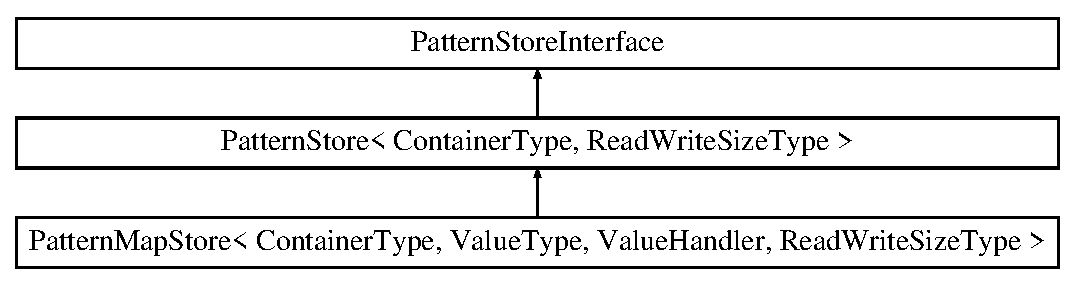
\includegraphics[height=2.921739cm]{classPatternStore}
\end{center}
\end{figure}
\subsection*{Public Types}
\begin{DoxyCompactItemize}
\item 
typedef Container\+Type\+::iterator \hyperlink{classPatternStore_ac0c35c2f256738575a5fc6932546d9dc}{iterator}
\item 
typedef Container\+Type\+::const\+\_\+iterator \hyperlink{classPatternStore_a605a2f6e75381eac263bcc36976c1377}{const\+\_\+iterator}
\end{DoxyCompactItemize}
\subsection*{Public Member Functions}
\begin{DoxyCompactItemize}
\item 
\hyperlink{classPatternStore_a8fc2f93bbac98093e3928423a9ef2fb6}{Pattern\+Store} ()
\item 
virtual \hyperlink{classPatternStore_ac4a1446d8c1637e34147dab4655e1bf1}{$\sim$\+Pattern\+Store} ()
\item 
virtual void \hyperlink{classPatternStore_a6e4361163bb2568593a5049f214a17b5}{attachcorpus} (unsigned char $\ast$\hyperlink{classPatternStore_a56811e603e5a5ce165a8709216f3f1c5}{corpusstart}, unsigned int \hyperlink{classPatternStore_aae8c0f162986134d629b0e6b1a63b4cc}{corpussize})
\item 
virtual void \hyperlink{classPatternStore_a38c362e35c48cf8a29b9a91bc9545cd3}{attachcorpus} (const \hyperlink{classIndexedCorpus}{Indexed\+Corpus} \&corpus)
\item 
virtual void \hyperlink{classPatternStore_a07493b7e476f3d59539ac7be0c811412}{detachcorpus} ()
\item 
unsigned char $\ast$ \hyperlink{classPatternStore_a53c9f6c2ef894c4ea871471d6b259d55}{getcorpus} () const 
\item 
unsigned int \hyperlink{classPatternStore_a409a492f79640da8eef56b089504191d}{getcorpussize} () const 
\item 
virtual void \hyperlink{classPatternStore_af82a73cc05a22318f86daee0e4ae5189}{use\+\_\+v1\+\_\+format} ()
\item 
virtual void \hyperlink{classPatternStore_aac1558cd3f7e4ec8ec142e1c59f122c9}{insert} (const \hyperlink{pattern_8h_a351dc5aa88481a949638aeb6cc5e6754}{Pattern\+Type} \&pattern)=0
\item 
virtual bool \hyperlink{classPatternStore_a2e29add9b35b3459d183f56f6c5525ed}{has} (const \hyperlink{classPattern}{Pattern} \&) const  =0
\item 
virtual bool \hyperlink{classPatternStore_ad1e06c2468bad2a14d4ed28b26c6ff33}{has} (const \hyperlink{classPatternPointer}{Pattern\+Pointer} \&) const  =0
\item 
virtual bool \hyperlink{classPatternStore_a42f8de80a8627c485315e4bb8eff538f}{erase} (const \hyperlink{pattern_8h_a351dc5aa88481a949638aeb6cc5e6754}{Pattern\+Type} \&)=0
\item 
virtual size\+\_\+t \hyperlink{classPatternStore_abfa82df94ab565bea13fc45ee4866faf}{size} () const  =0
\item 
virtual void \hyperlink{classPatternStore_afc995f7b88b6a31b700bb3bdb948b180}{reserve} (size\+\_\+t)=0
\item 
virtual Container\+Type\+::iterator \hyperlink{classPatternStore_aab3fab217b585b2b90a3fb3cc7065e11}{begin} ()=0
\item 
virtual Container\+Type\+::iterator \hyperlink{classPatternStore_ae697b6ba815e09fa300532a78e1c9077}{end} ()=0
\item 
virtual Container\+Type\+::iterator \hyperlink{classPatternStore_a6996798c63c2dd3ae3845848da35a6dd}{find} (const \hyperlink{classPattern}{Pattern} \&pattern)=0
\item 
virtual Container\+Type\+::iterator \hyperlink{classPatternStore_a33991d30a74b13a4264200474bf0542c}{find} (const \hyperlink{classPatternPointer}{Pattern\+Pointer} \&pattern)=0
\item 
virtual void \hyperlink{classPatternStore_a70d9b8faa5858ab7182cea7b1488a75c}{write} (std\+::ostream $\ast$out)=0
\item 
virtual \hyperlink{classPatternStoreInterface}{Pattern\+Store\+Interface} $\ast$ \hyperlink{classPatternStore_acd6094fb1e3fd4c655603dccdaed4c88}{getstoreinterface} ()
\end{DoxyCompactItemize}
\subsection*{Protected Attributes}
\begin{DoxyCompactItemize}
\item 
unsigned char $\ast$ \hyperlink{classPatternStore_a56811e603e5a5ce165a8709216f3f1c5}{corpusstart}
\item 
unsigned int \hyperlink{classPatternStore_aae8c0f162986134d629b0e6b1a63b4cc}{corpussize}
\item 
unsigned char \hyperlink{classPatternStore_a37f196867dede75f7a9bf72b07a3c24d}{classencodingversion}
\item 
int \hyperlink{classPatternStore_aa4ef383cb01f6842e97be70bea0e8c82}{patterntype}
\end{DoxyCompactItemize}


\subsection{Detailed Description}
\subsubsection*{template$<$class Container\+Type, class Read\+Write\+Size\+Type = uint64\+\_\+t, class Pattern\+Type = Pattern$>$class Pattern\+Store$<$ Container\+Type, Read\+Write\+Size\+Type, Pattern\+Type $>$}

Abstract \hyperlink{classPattern}{Pattern} store class, not to be instantiated directly. 

This is an abstract class, all \hyperlink{classPattern}{Pattern} storage containers are derived from this. 
\begin{DoxyTemplParams}{Template Parameters}
{\em Container\+Type} & The low-\/level container type used (an S\+T\+L container such as set/map). \\
\hline
{\em Read\+Write\+Size\+Type} & Data type for addressing, influences only the maximum number of items that can be stored (2$\ast$$\ast$64) in the container, as this will be represented in the very beginning of the binary file. No reason to change this unless the container is very deeply nested in others and contains only few items. \\
\hline
\end{DoxyTemplParams}


\subsection{Member Typedef Documentation}
\hypertarget{classPatternStore_a605a2f6e75381eac263bcc36976c1377}{}\index{Pattern\+Store@{Pattern\+Store}!const\+\_\+iterator@{const\+\_\+iterator}}
\index{const\+\_\+iterator@{const\+\_\+iterator}!Pattern\+Store@{Pattern\+Store}}
\subsubsection[{const\+\_\+iterator}]{\setlength{\rightskip}{0pt plus 5cm}template$<$class Container\+Type, class Read\+Write\+Size\+Type = uint64\+\_\+t, class Pattern\+Type = Pattern$>$ typedef Container\+Type\+::const\+\_\+iterator {\bf Pattern\+Store}$<$ Container\+Type, Read\+Write\+Size\+Type, {\bf Pattern\+Type} $>$\+::{\bf const\+\_\+iterator}}\label{classPatternStore_a605a2f6e75381eac263bcc36976c1377}
\hypertarget{classPatternStore_ac0c35c2f256738575a5fc6932546d9dc}{}\index{Pattern\+Store@{Pattern\+Store}!iterator@{iterator}}
\index{iterator@{iterator}!Pattern\+Store@{Pattern\+Store}}
\subsubsection[{iterator}]{\setlength{\rightskip}{0pt plus 5cm}template$<$class Container\+Type, class Read\+Write\+Size\+Type = uint64\+\_\+t, class Pattern\+Type = Pattern$>$ typedef Container\+Type\+::iterator {\bf Pattern\+Store}$<$ Container\+Type, Read\+Write\+Size\+Type, {\bf Pattern\+Type} $>$\+::{\bf iterator}}\label{classPatternStore_ac0c35c2f256738575a5fc6932546d9dc}


\subsection{Constructor \& Destructor Documentation}
\hypertarget{classPatternStore_a8fc2f93bbac98093e3928423a9ef2fb6}{}\index{Pattern\+Store@{Pattern\+Store}!Pattern\+Store@{Pattern\+Store}}
\index{Pattern\+Store@{Pattern\+Store}!Pattern\+Store@{Pattern\+Store}}
\subsubsection[{Pattern\+Store()}]{\setlength{\rightskip}{0pt plus 5cm}template$<$class Container\+Type, class Read\+Write\+Size\+Type = uint64\+\_\+t, class Pattern\+Type = Pattern$>$ {\bf Pattern\+Store}$<$ Container\+Type, Read\+Write\+Size\+Type, {\bf Pattern\+Type} $>$\+::{\bf Pattern\+Store} (
\begin{DoxyParamCaption}
{}
\end{DoxyParamCaption}
)\hspace{0.3cm}{\ttfamily [inline]}}\label{classPatternStore_a8fc2f93bbac98093e3928423a9ef2fb6}
\hypertarget{classPatternStore_ac4a1446d8c1637e34147dab4655e1bf1}{}\index{Pattern\+Store@{Pattern\+Store}!````~Pattern\+Store@{$\sim$\+Pattern\+Store}}
\index{````~Pattern\+Store@{$\sim$\+Pattern\+Store}!Pattern\+Store@{Pattern\+Store}}
\subsubsection[{$\sim$\+Pattern\+Store()}]{\setlength{\rightskip}{0pt plus 5cm}template$<$class Container\+Type, class Read\+Write\+Size\+Type = uint64\+\_\+t, class Pattern\+Type = Pattern$>$ virtual {\bf Pattern\+Store}$<$ Container\+Type, Read\+Write\+Size\+Type, {\bf Pattern\+Type} $>$\+::$\sim${\bf Pattern\+Store} (
\begin{DoxyParamCaption}
{}
\end{DoxyParamCaption}
)\hspace{0.3cm}{\ttfamily [inline]}, {\ttfamily [virtual]}}\label{classPatternStore_ac4a1446d8c1637e34147dab4655e1bf1}


\subsection{Member Function Documentation}
\hypertarget{classPatternStore_a6e4361163bb2568593a5049f214a17b5}{}\index{Pattern\+Store@{Pattern\+Store}!attachcorpus@{attachcorpus}}
\index{attachcorpus@{attachcorpus}!Pattern\+Store@{Pattern\+Store}}
\subsubsection[{attachcorpus(unsigned char $\ast$corpusstart, unsigned int corpussize)}]{\setlength{\rightskip}{0pt plus 5cm}template$<$class Container\+Type, class Read\+Write\+Size\+Type = uint64\+\_\+t, class Pattern\+Type = Pattern$>$ virtual void {\bf Pattern\+Store}$<$ Container\+Type, Read\+Write\+Size\+Type, {\bf Pattern\+Type} $>$\+::attachcorpus (
\begin{DoxyParamCaption}
\item[{unsigned char $\ast$}]{corpusstart, }
\item[{unsigned int}]{corpussize}
\end{DoxyParamCaption}
)\hspace{0.3cm}{\ttfamily [inline]}, {\ttfamily [virtual]}}\label{classPatternStore_a6e4361163bb2568593a5049f214a17b5}
\hypertarget{classPatternStore_a38c362e35c48cf8a29b9a91bc9545cd3}{}\index{Pattern\+Store@{Pattern\+Store}!attachcorpus@{attachcorpus}}
\index{attachcorpus@{attachcorpus}!Pattern\+Store@{Pattern\+Store}}
\subsubsection[{attachcorpus(const Indexed\+Corpus \&corpus)}]{\setlength{\rightskip}{0pt plus 5cm}template$<$class Container\+Type, class Read\+Write\+Size\+Type = uint64\+\_\+t, class Pattern\+Type = Pattern$>$ virtual void {\bf Pattern\+Store}$<$ Container\+Type, Read\+Write\+Size\+Type, {\bf Pattern\+Type} $>$\+::attachcorpus (
\begin{DoxyParamCaption}
\item[{const {\bf Indexed\+Corpus} \&}]{corpus}
\end{DoxyParamCaption}
)\hspace{0.3cm}{\ttfamily [inline]}, {\ttfamily [virtual]}}\label{classPatternStore_a38c362e35c48cf8a29b9a91bc9545cd3}
\hypertarget{classPatternStore_aab3fab217b585b2b90a3fb3cc7065e11}{}\index{Pattern\+Store@{Pattern\+Store}!begin@{begin}}
\index{begin@{begin}!Pattern\+Store@{Pattern\+Store}}
\subsubsection[{begin()=0}]{\setlength{\rightskip}{0pt plus 5cm}template$<$class Container\+Type, class Read\+Write\+Size\+Type = uint64\+\_\+t, class Pattern\+Type = Pattern$>$ virtual Container\+Type\+::iterator {\bf Pattern\+Store}$<$ Container\+Type, Read\+Write\+Size\+Type, {\bf Pattern\+Type} $>$\+::begin (
\begin{DoxyParamCaption}
{}
\end{DoxyParamCaption}
)\hspace{0.3cm}{\ttfamily [pure virtual]}}\label{classPatternStore_aab3fab217b585b2b90a3fb3cc7065e11}


Implemented in \hyperlink{classHashOrderedPatternMap_ac103913725b7036ba414453b2204b955}{Hash\+Ordered\+Pattern\+Map$<$ Value\+Type, Value\+Handler, Read\+Write\+Size\+Type $>$}, \hyperlink{classOrderedPatternPointerMap_a12194a18d92e1ddf107cbdbc59c8de65}{Ordered\+Pattern\+Pointer\+Map$<$ Value\+Type, Value\+Handler, Read\+Write\+Size\+Type $>$}, \hyperlink{classPatternPointerMap_ab27caf6f73f4c66ffb8399c72aee53a4}{Pattern\+Pointer\+Map$<$ Value\+Type, Value\+Handler, Read\+Write\+Size\+Type $>$}, \hyperlink{classPatternMap_a6e536f5947c4e1752f91166922c4ae16}{Pattern\+Map$<$ Value\+Type, Value\+Handler, Read\+Write\+Size\+Type $>$}, \hyperlink{classPatternMap_a6e536f5947c4e1752f91166922c4ae16}{Pattern\+Map$<$ Pattern\+Map$<$ Value\+Type, Value\+Handler, Nested\+Size\+Type $>$, Pattern\+Store\+Value\+Handler$<$ Pattern\+Map$<$ Value\+Type, Value\+Handler, Nested\+Size\+Type $>$ $>$, uint64\+\_\+t $>$}, \hyperlink{classPatternMap_a6e536f5947c4e1752f91166922c4ae16}{Pattern\+Map$<$ Value\+Type, Value\+Handler, Nested\+Size\+Type $>$}, \hyperlink{classPatternMap_a6e536f5947c4e1752f91166922c4ae16}{Pattern\+Map$<$ Pattern\+Feature\+Vector\+Map$<$ Feature\+Type $>$, Pattern\+Feature\+Vector\+Map\+Handler$<$ Feature\+Type $>$ $>$}, \hyperlink{classHashOrderedPatternSet_a94bf915d870e33639c80839d7da7ce54}{Hash\+Ordered\+Pattern\+Set$<$ Read\+Write\+Size\+Type $>$}, \hyperlink{classPatternSet_ac8c206e63c54d45443a38df762cea863}{Pattern\+Set$<$ Read\+Write\+Size\+Type $>$}, \hyperlink{classPatternSet_ac8c206e63c54d45443a38df762cea863}{Pattern\+Set$<$ uint64\+\_\+t $>$}, \hyperlink{classPatternMapStore_a34918a8855a815fcfda852888e7639bc}{Pattern\+Map\+Store$<$ Container\+Type, Value\+Type, Value\+Handler, Read\+Write\+Size\+Type, Pattern\+Type $>$}, \hyperlink{classPatternMapStore_a34918a8855a815fcfda852888e7639bc}{Pattern\+Map\+Store$<$ std\+::map$<$ Pattern\+Pointer, Value\+Type $>$, Value\+Type, Value\+Handler, Read\+Write\+Size\+Type, Pattern\+Pointer $>$}, \hyperlink{classPatternMapStore_a34918a8855a815fcfda852888e7639bc}{Pattern\+Map\+Store$<$ std\+::unordered\+\_\+map$<$ Pattern, Value\+Type $>$, Value\+Type, Value\+Handler, Nested\+Size\+Type, Pattern $>$}, \hyperlink{classPatternMapStore_a34918a8855a815fcfda852888e7639bc}{Pattern\+Map\+Store$<$ std\+::unordered\+\_\+map$<$ Pattern, Pattern\+Map$<$ Value\+Type, Value\+Handler, Nested\+Size\+Type $>$ $>$, Pattern\+Map$<$ Value\+Type, Value\+Handler, Nested\+Size\+Type $>$, Pattern\+Store\+Value\+Handler$<$ Pattern\+Map$<$ Value\+Type, Value\+Handler, Nested\+Size\+Type $>$ $>$, uint64\+\_\+t, Pattern $>$}, \hyperlink{classPatternMapStore_a34918a8855a815fcfda852888e7639bc}{Pattern\+Map\+Store$<$ std\+::unordered\+\_\+map$<$ Pattern, Value\+Type $>$, Value\+Type, Value\+Handler, Read\+Write\+Size\+Type, Pattern $>$}, \hyperlink{classPatternMapStore_a34918a8855a815fcfda852888e7639bc}{Pattern\+Map\+Store$<$ std\+::unordered\+\_\+map$<$ Pattern\+Pointer, Value\+Type $>$, Value\+Type, Value\+Handler, Read\+Write\+Size\+Type, Pattern\+Pointer $>$}, \hyperlink{classPatternMapStore_a34918a8855a815fcfda852888e7639bc}{Pattern\+Map\+Store$<$ std\+::unordered\+\_\+map$<$ Pattern, Pattern\+Feature\+Vector\+Map$<$ Feature\+Type $>$ $>$, Pattern\+Feature\+Vector\+Map$<$ Feature\+Type $>$, Pattern\+Feature\+Vector\+Map\+Handler$<$ Feature\+Type $>$, uint64\+\_\+t, Pattern $>$}, and \hyperlink{classPatternMapStore_a34918a8855a815fcfda852888e7639bc}{Pattern\+Map\+Store$<$ std\+::map$<$ const Pattern, Value\+Type $>$, Value\+Type, Value\+Handler, Read\+Write\+Size\+Type, Pattern $>$}.

\hypertarget{classPatternStore_a07493b7e476f3d59539ac7be0c811412}{}\index{Pattern\+Store@{Pattern\+Store}!detachcorpus@{detachcorpus}}
\index{detachcorpus@{detachcorpus}!Pattern\+Store@{Pattern\+Store}}
\subsubsection[{detachcorpus()}]{\setlength{\rightskip}{0pt plus 5cm}template$<$class Container\+Type, class Read\+Write\+Size\+Type = uint64\+\_\+t, class Pattern\+Type = Pattern$>$ virtual void {\bf Pattern\+Store}$<$ Container\+Type, Read\+Write\+Size\+Type, {\bf Pattern\+Type} $>$\+::detachcorpus (
\begin{DoxyParamCaption}
{}
\end{DoxyParamCaption}
)\hspace{0.3cm}{\ttfamily [inline]}, {\ttfamily [virtual]}}\label{classPatternStore_a07493b7e476f3d59539ac7be0c811412}
\hypertarget{classPatternStore_ae697b6ba815e09fa300532a78e1c9077}{}\index{Pattern\+Store@{Pattern\+Store}!end@{end}}
\index{end@{end}!Pattern\+Store@{Pattern\+Store}}
\subsubsection[{end()=0}]{\setlength{\rightskip}{0pt plus 5cm}template$<$class Container\+Type, class Read\+Write\+Size\+Type = uint64\+\_\+t, class Pattern\+Type = Pattern$>$ virtual Container\+Type\+::iterator {\bf Pattern\+Store}$<$ Container\+Type, Read\+Write\+Size\+Type, {\bf Pattern\+Type} $>$\+::end (
\begin{DoxyParamCaption}
{}
\end{DoxyParamCaption}
)\hspace{0.3cm}{\ttfamily [pure virtual]}}\label{classPatternStore_ae697b6ba815e09fa300532a78e1c9077}


Implemented in \hyperlink{classHashOrderedPatternMap_aa2a8090eed690299d4abeb36ea16fb3d}{Hash\+Ordered\+Pattern\+Map$<$ Value\+Type, Value\+Handler, Read\+Write\+Size\+Type $>$}, \hyperlink{classOrderedPatternPointerMap_a6e930ff1ee953bc901323746c5e418ca}{Ordered\+Pattern\+Pointer\+Map$<$ Value\+Type, Value\+Handler, Read\+Write\+Size\+Type $>$}, \hyperlink{classPatternPointerMap_abc9e82948004438795cf5c417147b375}{Pattern\+Pointer\+Map$<$ Value\+Type, Value\+Handler, Read\+Write\+Size\+Type $>$}, \hyperlink{classPatternMap_aa5a92eab727e74e54b93f7f7916e26cb}{Pattern\+Map$<$ Value\+Type, Value\+Handler, Read\+Write\+Size\+Type $>$}, \hyperlink{classPatternMap_aa5a92eab727e74e54b93f7f7916e26cb}{Pattern\+Map$<$ Pattern\+Map$<$ Value\+Type, Value\+Handler, Nested\+Size\+Type $>$, Pattern\+Store\+Value\+Handler$<$ Pattern\+Map$<$ Value\+Type, Value\+Handler, Nested\+Size\+Type $>$ $>$, uint64\+\_\+t $>$}, \hyperlink{classPatternMap_aa5a92eab727e74e54b93f7f7916e26cb}{Pattern\+Map$<$ Value\+Type, Value\+Handler, Nested\+Size\+Type $>$}, \hyperlink{classPatternMap_aa5a92eab727e74e54b93f7f7916e26cb}{Pattern\+Map$<$ Pattern\+Feature\+Vector\+Map$<$ Feature\+Type $>$, Pattern\+Feature\+Vector\+Map\+Handler$<$ Feature\+Type $>$ $>$}, \hyperlink{classHashOrderedPatternSet_ada3bb2f1617443ad288c5c22dcd33ec0}{Hash\+Ordered\+Pattern\+Set$<$ Read\+Write\+Size\+Type $>$}, \hyperlink{classPatternSet_a8ef5ec893a3ab9b00cf70cfdf2e623b9}{Pattern\+Set$<$ Read\+Write\+Size\+Type $>$}, \hyperlink{classPatternSet_a8ef5ec893a3ab9b00cf70cfdf2e623b9}{Pattern\+Set$<$ uint64\+\_\+t $>$}, \hyperlink{classPatternMapStore_a81b765692da54406e3951e1e1ae84fa5}{Pattern\+Map\+Store$<$ Container\+Type, Value\+Type, Value\+Handler, Read\+Write\+Size\+Type, Pattern\+Type $>$}, \hyperlink{classPatternMapStore_a81b765692da54406e3951e1e1ae84fa5}{Pattern\+Map\+Store$<$ std\+::map$<$ Pattern\+Pointer, Value\+Type $>$, Value\+Type, Value\+Handler, Read\+Write\+Size\+Type, Pattern\+Pointer $>$}, \hyperlink{classPatternMapStore_a81b765692da54406e3951e1e1ae84fa5}{Pattern\+Map\+Store$<$ std\+::unordered\+\_\+map$<$ Pattern, Value\+Type $>$, Value\+Type, Value\+Handler, Nested\+Size\+Type, Pattern $>$}, \hyperlink{classPatternMapStore_a81b765692da54406e3951e1e1ae84fa5}{Pattern\+Map\+Store$<$ std\+::unordered\+\_\+map$<$ Pattern, Pattern\+Map$<$ Value\+Type, Value\+Handler, Nested\+Size\+Type $>$ $>$, Pattern\+Map$<$ Value\+Type, Value\+Handler, Nested\+Size\+Type $>$, Pattern\+Store\+Value\+Handler$<$ Pattern\+Map$<$ Value\+Type, Value\+Handler, Nested\+Size\+Type $>$ $>$, uint64\+\_\+t, Pattern $>$}, \hyperlink{classPatternMapStore_a81b765692da54406e3951e1e1ae84fa5}{Pattern\+Map\+Store$<$ std\+::unordered\+\_\+map$<$ Pattern, Value\+Type $>$, Value\+Type, Value\+Handler, Read\+Write\+Size\+Type, Pattern $>$}, \hyperlink{classPatternMapStore_a81b765692da54406e3951e1e1ae84fa5}{Pattern\+Map\+Store$<$ std\+::unordered\+\_\+map$<$ Pattern\+Pointer, Value\+Type $>$, Value\+Type, Value\+Handler, Read\+Write\+Size\+Type, Pattern\+Pointer $>$}, \hyperlink{classPatternMapStore_a81b765692da54406e3951e1e1ae84fa5}{Pattern\+Map\+Store$<$ std\+::unordered\+\_\+map$<$ Pattern, Pattern\+Feature\+Vector\+Map$<$ Feature\+Type $>$ $>$, Pattern\+Feature\+Vector\+Map$<$ Feature\+Type $>$, Pattern\+Feature\+Vector\+Map\+Handler$<$ Feature\+Type $>$, uint64\+\_\+t, Pattern $>$}, and \hyperlink{classPatternMapStore_a81b765692da54406e3951e1e1ae84fa5}{Pattern\+Map\+Store$<$ std\+::map$<$ const Pattern, Value\+Type $>$, Value\+Type, Value\+Handler, Read\+Write\+Size\+Type, Pattern $>$}.

\hypertarget{classPatternStore_a42f8de80a8627c485315e4bb8eff538f}{}\index{Pattern\+Store@{Pattern\+Store}!erase@{erase}}
\index{erase@{erase}!Pattern\+Store@{Pattern\+Store}}
\subsubsection[{erase(const Pattern\+Type \&)=0}]{\setlength{\rightskip}{0pt plus 5cm}template$<$class Container\+Type, class Read\+Write\+Size\+Type = uint64\+\_\+t, class Pattern\+Type = Pattern$>$ virtual bool {\bf Pattern\+Store}$<$ Container\+Type, Read\+Write\+Size\+Type, {\bf Pattern\+Type} $>$\+::erase (
\begin{DoxyParamCaption}
\item[{const {\bf Pattern\+Type} \&}]{}
\end{DoxyParamCaption}
)\hspace{0.3cm}{\ttfamily [pure virtual]}}\label{classPatternStore_a42f8de80a8627c485315e4bb8eff538f}


Implemented in \hyperlink{classHashOrderedPatternMap_acc3231c8b727c982ef11c80d3390f8ec}{Hash\+Ordered\+Pattern\+Map$<$ Value\+Type, Value\+Handler, Read\+Write\+Size\+Type $>$}, \hyperlink{classOrderedPatternPointerMap_afadff7b0e87659c39dec96c16649fcb8}{Ordered\+Pattern\+Pointer\+Map$<$ Value\+Type, Value\+Handler, Read\+Write\+Size\+Type $>$}, \hyperlink{classPatternPointerMap_ac6c8adf867fa872c8677ed8a65e4e6d9}{Pattern\+Pointer\+Map$<$ Value\+Type, Value\+Handler, Read\+Write\+Size\+Type $>$}, \hyperlink{classPatternMap_a96e5a77a5c782f340fe38f5c05ae30c4}{Pattern\+Map$<$ Value\+Type, Value\+Handler, Read\+Write\+Size\+Type $>$}, \hyperlink{classPatternMap_a96e5a77a5c782f340fe38f5c05ae30c4}{Pattern\+Map$<$ Pattern\+Map$<$ Value\+Type, Value\+Handler, Nested\+Size\+Type $>$, Pattern\+Store\+Value\+Handler$<$ Pattern\+Map$<$ Value\+Type, Value\+Handler, Nested\+Size\+Type $>$ $>$, uint64\+\_\+t $>$}, \hyperlink{classPatternMap_a96e5a77a5c782f340fe38f5c05ae30c4}{Pattern\+Map$<$ Value\+Type, Value\+Handler, Nested\+Size\+Type $>$}, \hyperlink{classPatternMap_a96e5a77a5c782f340fe38f5c05ae30c4}{Pattern\+Map$<$ Pattern\+Feature\+Vector\+Map$<$ Feature\+Type $>$, Pattern\+Feature\+Vector\+Map\+Handler$<$ Feature\+Type $>$ $>$}, \hyperlink{classHashOrderedPatternSet_ab48e2380fcc00d9dc0ef01d9217fb5e6}{Hash\+Ordered\+Pattern\+Set$<$ Read\+Write\+Size\+Type $>$}, \hyperlink{classPatternSet_afd2c053ac589e30edd7eda5c9f95c771}{Pattern\+Set$<$ Read\+Write\+Size\+Type $>$}, \hyperlink{classPatternSet_afd2c053ac589e30edd7eda5c9f95c771}{Pattern\+Set$<$ uint64\+\_\+t $>$}, \hyperlink{classPatternMapStore_a1cd3996a4d1067783adb0ce4100d5f38}{Pattern\+Map\+Store$<$ Container\+Type, Value\+Type, Value\+Handler, Read\+Write\+Size\+Type, Pattern\+Type $>$}, \hyperlink{classPatternMapStore_a1cd3996a4d1067783adb0ce4100d5f38}{Pattern\+Map\+Store$<$ std\+::map$<$ Pattern\+Pointer, Value\+Type $>$, Value\+Type, Value\+Handler, Read\+Write\+Size\+Type, Pattern\+Pointer $>$}, \hyperlink{classPatternMapStore_a1cd3996a4d1067783adb0ce4100d5f38}{Pattern\+Map\+Store$<$ std\+::unordered\+\_\+map$<$ Pattern, Value\+Type $>$, Value\+Type, Value\+Handler, Nested\+Size\+Type, Pattern $>$}, \hyperlink{classPatternMapStore_a1cd3996a4d1067783adb0ce4100d5f38}{Pattern\+Map\+Store$<$ std\+::unordered\+\_\+map$<$ Pattern, Pattern\+Map$<$ Value\+Type, Value\+Handler, Nested\+Size\+Type $>$ $>$, Pattern\+Map$<$ Value\+Type, Value\+Handler, Nested\+Size\+Type $>$, Pattern\+Store\+Value\+Handler$<$ Pattern\+Map$<$ Value\+Type, Value\+Handler, Nested\+Size\+Type $>$ $>$, uint64\+\_\+t, Pattern $>$}, \hyperlink{classPatternMapStore_a1cd3996a4d1067783adb0ce4100d5f38}{Pattern\+Map\+Store$<$ std\+::unordered\+\_\+map$<$ Pattern, Value\+Type $>$, Value\+Type, Value\+Handler, Read\+Write\+Size\+Type, Pattern $>$}, \hyperlink{classPatternMapStore_a1cd3996a4d1067783adb0ce4100d5f38}{Pattern\+Map\+Store$<$ std\+::unordered\+\_\+map$<$ Pattern\+Pointer, Value\+Type $>$, Value\+Type, Value\+Handler, Read\+Write\+Size\+Type, Pattern\+Pointer $>$}, \hyperlink{classPatternMapStore_a1cd3996a4d1067783adb0ce4100d5f38}{Pattern\+Map\+Store$<$ std\+::unordered\+\_\+map$<$ Pattern, Pattern\+Feature\+Vector\+Map$<$ Feature\+Type $>$ $>$, Pattern\+Feature\+Vector\+Map$<$ Feature\+Type $>$, Pattern\+Feature\+Vector\+Map\+Handler$<$ Feature\+Type $>$, uint64\+\_\+t, Pattern $>$}, and \hyperlink{classPatternMapStore_a1cd3996a4d1067783adb0ce4100d5f38}{Pattern\+Map\+Store$<$ std\+::map$<$ const Pattern, Value\+Type $>$, Value\+Type, Value\+Handler, Read\+Write\+Size\+Type, Pattern $>$}.

\hypertarget{classPatternStore_a6996798c63c2dd3ae3845848da35a6dd}{}\index{Pattern\+Store@{Pattern\+Store}!find@{find}}
\index{find@{find}!Pattern\+Store@{Pattern\+Store}}
\subsubsection[{find(const Pattern \&pattern)=0}]{\setlength{\rightskip}{0pt plus 5cm}template$<$class Container\+Type, class Read\+Write\+Size\+Type = uint64\+\_\+t, class Pattern\+Type = Pattern$>$ virtual Container\+Type\+::iterator {\bf Pattern\+Store}$<$ Container\+Type, Read\+Write\+Size\+Type, {\bf Pattern\+Type} $>$\+::find (
\begin{DoxyParamCaption}
\item[{const {\bf Pattern} \&}]{pattern}
\end{DoxyParamCaption}
)\hspace{0.3cm}{\ttfamily [pure virtual]}}\label{classPatternStore_a6996798c63c2dd3ae3845848da35a6dd}


Implemented in \hyperlink{classHashOrderedPatternMap_ab0391b67630d9c20ee0069f7197ca9da}{Hash\+Ordered\+Pattern\+Map$<$ Value\+Type, Value\+Handler, Read\+Write\+Size\+Type $>$}, \hyperlink{classOrderedPatternPointerMap_a19bdc5b4b028c8c89638d263cbe168ab}{Ordered\+Pattern\+Pointer\+Map$<$ Value\+Type, Value\+Handler, Read\+Write\+Size\+Type $>$}, \hyperlink{classPatternPointerMap_af4971cbafd7193d03ad46823e7bde0af}{Pattern\+Pointer\+Map$<$ Value\+Type, Value\+Handler, Read\+Write\+Size\+Type $>$}, \hyperlink{classPatternMap_a4f36d73514e80d18f93395a72f81e6bc}{Pattern\+Map$<$ Value\+Type, Value\+Handler, Read\+Write\+Size\+Type $>$}, \hyperlink{classPatternMap_a4f36d73514e80d18f93395a72f81e6bc}{Pattern\+Map$<$ Pattern\+Map$<$ Value\+Type, Value\+Handler, Nested\+Size\+Type $>$, Pattern\+Store\+Value\+Handler$<$ Pattern\+Map$<$ Value\+Type, Value\+Handler, Nested\+Size\+Type $>$ $>$, uint64\+\_\+t $>$}, \hyperlink{classPatternMap_a4f36d73514e80d18f93395a72f81e6bc}{Pattern\+Map$<$ Value\+Type, Value\+Handler, Nested\+Size\+Type $>$}, \hyperlink{classPatternMap_a4f36d73514e80d18f93395a72f81e6bc}{Pattern\+Map$<$ Pattern\+Feature\+Vector\+Map$<$ Feature\+Type $>$, Pattern\+Feature\+Vector\+Map\+Handler$<$ Feature\+Type $>$ $>$}, \hyperlink{classHashOrderedPatternSet_aaf005777860a7af872aa104b1b7f9895}{Hash\+Ordered\+Pattern\+Set$<$ Read\+Write\+Size\+Type $>$}, \hyperlink{classPatternSet_a2c56aa5b266f2132f8453bf794bba1f5}{Pattern\+Set$<$ Read\+Write\+Size\+Type $>$}, \hyperlink{classPatternSet_a2c56aa5b266f2132f8453bf794bba1f5}{Pattern\+Set$<$ uint64\+\_\+t $>$}, \hyperlink{classPatternMapStore_abe0af4c950b2389e5ec7c4d5bfb759c7}{Pattern\+Map\+Store$<$ Container\+Type, Value\+Type, Value\+Handler, Read\+Write\+Size\+Type, Pattern\+Type $>$}, \hyperlink{classPatternMapStore_abe0af4c950b2389e5ec7c4d5bfb759c7}{Pattern\+Map\+Store$<$ std\+::map$<$ Pattern\+Pointer, Value\+Type $>$, Value\+Type, Value\+Handler, Read\+Write\+Size\+Type, Pattern\+Pointer $>$}, \hyperlink{classPatternMapStore_abe0af4c950b2389e5ec7c4d5bfb759c7}{Pattern\+Map\+Store$<$ std\+::unordered\+\_\+map$<$ Pattern, Value\+Type $>$, Value\+Type, Value\+Handler, Nested\+Size\+Type, Pattern $>$}, \hyperlink{classPatternMapStore_abe0af4c950b2389e5ec7c4d5bfb759c7}{Pattern\+Map\+Store$<$ std\+::unordered\+\_\+map$<$ Pattern, Pattern\+Map$<$ Value\+Type, Value\+Handler, Nested\+Size\+Type $>$ $>$, Pattern\+Map$<$ Value\+Type, Value\+Handler, Nested\+Size\+Type $>$, Pattern\+Store\+Value\+Handler$<$ Pattern\+Map$<$ Value\+Type, Value\+Handler, Nested\+Size\+Type $>$ $>$, uint64\+\_\+t, Pattern $>$}, \hyperlink{classPatternMapStore_abe0af4c950b2389e5ec7c4d5bfb759c7}{Pattern\+Map\+Store$<$ std\+::unordered\+\_\+map$<$ Pattern, Value\+Type $>$, Value\+Type, Value\+Handler, Read\+Write\+Size\+Type, Pattern $>$}, \hyperlink{classPatternMapStore_abe0af4c950b2389e5ec7c4d5bfb759c7}{Pattern\+Map\+Store$<$ std\+::unordered\+\_\+map$<$ Pattern\+Pointer, Value\+Type $>$, Value\+Type, Value\+Handler, Read\+Write\+Size\+Type, Pattern\+Pointer $>$}, \hyperlink{classPatternMapStore_abe0af4c950b2389e5ec7c4d5bfb759c7}{Pattern\+Map\+Store$<$ std\+::unordered\+\_\+map$<$ Pattern, Pattern\+Feature\+Vector\+Map$<$ Feature\+Type $>$ $>$, Pattern\+Feature\+Vector\+Map$<$ Feature\+Type $>$, Pattern\+Feature\+Vector\+Map\+Handler$<$ Feature\+Type $>$, uint64\+\_\+t, Pattern $>$}, and \hyperlink{classPatternMapStore_abe0af4c950b2389e5ec7c4d5bfb759c7}{Pattern\+Map\+Store$<$ std\+::map$<$ const Pattern, Value\+Type $>$, Value\+Type, Value\+Handler, Read\+Write\+Size\+Type, Pattern $>$}.

\hypertarget{classPatternStore_a33991d30a74b13a4264200474bf0542c}{}\index{Pattern\+Store@{Pattern\+Store}!find@{find}}
\index{find@{find}!Pattern\+Store@{Pattern\+Store}}
\subsubsection[{find(const Pattern\+Pointer \&pattern)=0}]{\setlength{\rightskip}{0pt plus 5cm}template$<$class Container\+Type, class Read\+Write\+Size\+Type = uint64\+\_\+t, class Pattern\+Type = Pattern$>$ virtual Container\+Type\+::iterator {\bf Pattern\+Store}$<$ Container\+Type, Read\+Write\+Size\+Type, {\bf Pattern\+Type} $>$\+::find (
\begin{DoxyParamCaption}
\item[{const {\bf Pattern\+Pointer} \&}]{pattern}
\end{DoxyParamCaption}
)\hspace{0.3cm}{\ttfamily [pure virtual]}}\label{classPatternStore_a33991d30a74b13a4264200474bf0542c}


Implemented in \hyperlink{classHashOrderedPatternMap_a1b1f8f29f6a967b945a7d22907890977}{Hash\+Ordered\+Pattern\+Map$<$ Value\+Type, Value\+Handler, Read\+Write\+Size\+Type $>$}, \hyperlink{classOrderedPatternPointerMap_a0fd55cda8460d3ad5dc3d67d9bc4e3ac}{Ordered\+Pattern\+Pointer\+Map$<$ Value\+Type, Value\+Handler, Read\+Write\+Size\+Type $>$}, \hyperlink{classPatternPointerMap_a722120c11af76500a453e68b35ca6d03}{Pattern\+Pointer\+Map$<$ Value\+Type, Value\+Handler, Read\+Write\+Size\+Type $>$}, \hyperlink{classPatternMap_a75e2cf7d74b8ffed73256324cfa1e3bf}{Pattern\+Map$<$ Value\+Type, Value\+Handler, Read\+Write\+Size\+Type $>$}, \hyperlink{classPatternMap_a75e2cf7d74b8ffed73256324cfa1e3bf}{Pattern\+Map$<$ Pattern\+Map$<$ Value\+Type, Value\+Handler, Nested\+Size\+Type $>$, Pattern\+Store\+Value\+Handler$<$ Pattern\+Map$<$ Value\+Type, Value\+Handler, Nested\+Size\+Type $>$ $>$, uint64\+\_\+t $>$}, \hyperlink{classPatternMap_a75e2cf7d74b8ffed73256324cfa1e3bf}{Pattern\+Map$<$ Value\+Type, Value\+Handler, Nested\+Size\+Type $>$}, \hyperlink{classPatternMap_a75e2cf7d74b8ffed73256324cfa1e3bf}{Pattern\+Map$<$ Pattern\+Feature\+Vector\+Map$<$ Feature\+Type $>$, Pattern\+Feature\+Vector\+Map\+Handler$<$ Feature\+Type $>$ $>$}, \hyperlink{classHashOrderedPatternSet_a90e6642ea5198c48bb23af9cee8f3b76}{Hash\+Ordered\+Pattern\+Set$<$ Read\+Write\+Size\+Type $>$}, \hyperlink{classPatternSet_a0463855da3729a70a59ee2e24265fbf8}{Pattern\+Set$<$ Read\+Write\+Size\+Type $>$}, \hyperlink{classPatternSet_a0463855da3729a70a59ee2e24265fbf8}{Pattern\+Set$<$ uint64\+\_\+t $>$}, \hyperlink{classPatternMapStore_aa09480df06716f8e2b22972636d48c9e}{Pattern\+Map\+Store$<$ Container\+Type, Value\+Type, Value\+Handler, Read\+Write\+Size\+Type, Pattern\+Type $>$}, \hyperlink{classPatternMapStore_aa09480df06716f8e2b22972636d48c9e}{Pattern\+Map\+Store$<$ std\+::map$<$ Pattern\+Pointer, Value\+Type $>$, Value\+Type, Value\+Handler, Read\+Write\+Size\+Type, Pattern\+Pointer $>$}, \hyperlink{classPatternMapStore_aa09480df06716f8e2b22972636d48c9e}{Pattern\+Map\+Store$<$ std\+::unordered\+\_\+map$<$ Pattern, Value\+Type $>$, Value\+Type, Value\+Handler, Nested\+Size\+Type, Pattern $>$}, \hyperlink{classPatternMapStore_aa09480df06716f8e2b22972636d48c9e}{Pattern\+Map\+Store$<$ std\+::unordered\+\_\+map$<$ Pattern, Pattern\+Map$<$ Value\+Type, Value\+Handler, Nested\+Size\+Type $>$ $>$, Pattern\+Map$<$ Value\+Type, Value\+Handler, Nested\+Size\+Type $>$, Pattern\+Store\+Value\+Handler$<$ Pattern\+Map$<$ Value\+Type, Value\+Handler, Nested\+Size\+Type $>$ $>$, uint64\+\_\+t, Pattern $>$}, \hyperlink{classPatternMapStore_aa09480df06716f8e2b22972636d48c9e}{Pattern\+Map\+Store$<$ std\+::unordered\+\_\+map$<$ Pattern, Value\+Type $>$, Value\+Type, Value\+Handler, Read\+Write\+Size\+Type, Pattern $>$}, \hyperlink{classPatternMapStore_aa09480df06716f8e2b22972636d48c9e}{Pattern\+Map\+Store$<$ std\+::unordered\+\_\+map$<$ Pattern\+Pointer, Value\+Type $>$, Value\+Type, Value\+Handler, Read\+Write\+Size\+Type, Pattern\+Pointer $>$}, \hyperlink{classPatternMapStore_aa09480df06716f8e2b22972636d48c9e}{Pattern\+Map\+Store$<$ std\+::unordered\+\_\+map$<$ Pattern, Pattern\+Feature\+Vector\+Map$<$ Feature\+Type $>$ $>$, Pattern\+Feature\+Vector\+Map$<$ Feature\+Type $>$, Pattern\+Feature\+Vector\+Map\+Handler$<$ Feature\+Type $>$, uint64\+\_\+t, Pattern $>$}, and \hyperlink{classPatternMapStore_aa09480df06716f8e2b22972636d48c9e}{Pattern\+Map\+Store$<$ std\+::map$<$ const Pattern, Value\+Type $>$, Value\+Type, Value\+Handler, Read\+Write\+Size\+Type, Pattern $>$}.

\hypertarget{classPatternStore_a53c9f6c2ef894c4ea871471d6b259d55}{}\index{Pattern\+Store@{Pattern\+Store}!getcorpus@{getcorpus}}
\index{getcorpus@{getcorpus}!Pattern\+Store@{Pattern\+Store}}
\subsubsection[{getcorpus() const }]{\setlength{\rightskip}{0pt plus 5cm}template$<$class Container\+Type, class Read\+Write\+Size\+Type = uint64\+\_\+t, class Pattern\+Type = Pattern$>$ unsigned char$\ast$ {\bf Pattern\+Store}$<$ Container\+Type, Read\+Write\+Size\+Type, {\bf Pattern\+Type} $>$\+::getcorpus (
\begin{DoxyParamCaption}
{}
\end{DoxyParamCaption}
) const\hspace{0.3cm}{\ttfamily [inline]}}\label{classPatternStore_a53c9f6c2ef894c4ea871471d6b259d55}
\hypertarget{classPatternStore_a409a492f79640da8eef56b089504191d}{}\index{Pattern\+Store@{Pattern\+Store}!getcorpussize@{getcorpussize}}
\index{getcorpussize@{getcorpussize}!Pattern\+Store@{Pattern\+Store}}
\subsubsection[{getcorpussize() const }]{\setlength{\rightskip}{0pt plus 5cm}template$<$class Container\+Type, class Read\+Write\+Size\+Type = uint64\+\_\+t, class Pattern\+Type = Pattern$>$ unsigned int {\bf Pattern\+Store}$<$ Container\+Type, Read\+Write\+Size\+Type, {\bf Pattern\+Type} $>$\+::getcorpussize (
\begin{DoxyParamCaption}
{}
\end{DoxyParamCaption}
) const\hspace{0.3cm}{\ttfamily [inline]}}\label{classPatternStore_a409a492f79640da8eef56b089504191d}
\hypertarget{classPatternStore_acd6094fb1e3fd4c655603dccdaed4c88}{}\index{Pattern\+Store@{Pattern\+Store}!getstoreinterface@{getstoreinterface}}
\index{getstoreinterface@{getstoreinterface}!Pattern\+Store@{Pattern\+Store}}
\subsubsection[{getstoreinterface()}]{\setlength{\rightskip}{0pt plus 5cm}template$<$class Container\+Type, class Read\+Write\+Size\+Type = uint64\+\_\+t, class Pattern\+Type = Pattern$>$ virtual {\bf Pattern\+Store\+Interface}$\ast$ {\bf Pattern\+Store}$<$ Container\+Type, Read\+Write\+Size\+Type, {\bf Pattern\+Type} $>$\+::getstoreinterface (
\begin{DoxyParamCaption}
{}
\end{DoxyParamCaption}
)\hspace{0.3cm}{\ttfamily [inline]}, {\ttfamily [virtual]}}\label{classPatternStore_acd6094fb1e3fd4c655603dccdaed4c88}
\hypertarget{classPatternStore_a2e29add9b35b3459d183f56f6c5525ed}{}\index{Pattern\+Store@{Pattern\+Store}!has@{has}}
\index{has@{has}!Pattern\+Store@{Pattern\+Store}}
\subsubsection[{has(const Pattern \&) const  =0}]{\setlength{\rightskip}{0pt plus 5cm}template$<$class Container\+Type, class Read\+Write\+Size\+Type = uint64\+\_\+t, class Pattern\+Type = Pattern$>$ virtual bool {\bf Pattern\+Store}$<$ Container\+Type, Read\+Write\+Size\+Type, {\bf Pattern\+Type} $>$\+::has (
\begin{DoxyParamCaption}
\item[{const {\bf Pattern} \&}]{}
\end{DoxyParamCaption}
) const\hspace{0.3cm}{\ttfamily [pure virtual]}}\label{classPatternStore_a2e29add9b35b3459d183f56f6c5525ed}
Does the pattern occur in the pattern store? 

Implements \hyperlink{classPatternStoreInterface_aec9f27496b38f8db1eced920fb2dc9fe}{Pattern\+Store\+Interface}.



Implemented in \hyperlink{classHashOrderedPatternMap_a8682c2810f85d0c80ed015e388b571ef}{Hash\+Ordered\+Pattern\+Map$<$ Value\+Type, Value\+Handler, Read\+Write\+Size\+Type $>$}, \hyperlink{classOrderedPatternPointerMap_a646cdbf8491700740207b8fd980fbcc7}{Ordered\+Pattern\+Pointer\+Map$<$ Value\+Type, Value\+Handler, Read\+Write\+Size\+Type $>$}, \hyperlink{classPatternPointerMap_aff90e9b372ae3aed68cb037d91f65206}{Pattern\+Pointer\+Map$<$ Value\+Type, Value\+Handler, Read\+Write\+Size\+Type $>$}, \hyperlink{classPatternMap_a038d49e8aed58a207c3e106b086cdab0}{Pattern\+Map$<$ Value\+Type, Value\+Handler, Read\+Write\+Size\+Type $>$}, \hyperlink{classPatternMap_a038d49e8aed58a207c3e106b086cdab0}{Pattern\+Map$<$ Pattern\+Map$<$ Value\+Type, Value\+Handler, Nested\+Size\+Type $>$, Pattern\+Store\+Value\+Handler$<$ Pattern\+Map$<$ Value\+Type, Value\+Handler, Nested\+Size\+Type $>$ $>$, uint64\+\_\+t $>$}, \hyperlink{classPatternMap_a038d49e8aed58a207c3e106b086cdab0}{Pattern\+Map$<$ Value\+Type, Value\+Handler, Nested\+Size\+Type $>$}, \hyperlink{classPatternMap_a038d49e8aed58a207c3e106b086cdab0}{Pattern\+Map$<$ Pattern\+Feature\+Vector\+Map$<$ Feature\+Type $>$, Pattern\+Feature\+Vector\+Map\+Handler$<$ Feature\+Type $>$ $>$}, \hyperlink{classHashOrderedPatternSet_ac21ec186302af16a3b70c5c85e434510}{Hash\+Ordered\+Pattern\+Set$<$ Read\+Write\+Size\+Type $>$}, \hyperlink{classPatternSet_a25e9ec9ca33750f21dd729cd2462d925}{Pattern\+Set$<$ Read\+Write\+Size\+Type $>$}, \hyperlink{classPatternSet_a25e9ec9ca33750f21dd729cd2462d925}{Pattern\+Set$<$ uint64\+\_\+t $>$}, \hyperlink{classPatternMapStore_a208cf2d90725a3a9291d2dae67ac9256}{Pattern\+Map\+Store$<$ Container\+Type, Value\+Type, Value\+Handler, Read\+Write\+Size\+Type, Pattern\+Type $>$}, \hyperlink{classPatternMapStore_a208cf2d90725a3a9291d2dae67ac9256}{Pattern\+Map\+Store$<$ std\+::map$<$ Pattern\+Pointer, Value\+Type $>$, Value\+Type, Value\+Handler, Read\+Write\+Size\+Type, Pattern\+Pointer $>$}, \hyperlink{classPatternMapStore_a208cf2d90725a3a9291d2dae67ac9256}{Pattern\+Map\+Store$<$ std\+::unordered\+\_\+map$<$ Pattern, Value\+Type $>$, Value\+Type, Value\+Handler, Nested\+Size\+Type, Pattern $>$}, \hyperlink{classPatternMapStore_a208cf2d90725a3a9291d2dae67ac9256}{Pattern\+Map\+Store$<$ std\+::unordered\+\_\+map$<$ Pattern, Pattern\+Map$<$ Value\+Type, Value\+Handler, Nested\+Size\+Type $>$ $>$, Pattern\+Map$<$ Value\+Type, Value\+Handler, Nested\+Size\+Type $>$, Pattern\+Store\+Value\+Handler$<$ Pattern\+Map$<$ Value\+Type, Value\+Handler, Nested\+Size\+Type $>$ $>$, uint64\+\_\+t, Pattern $>$}, \hyperlink{classPatternMapStore_a208cf2d90725a3a9291d2dae67ac9256}{Pattern\+Map\+Store$<$ std\+::unordered\+\_\+map$<$ Pattern, Value\+Type $>$, Value\+Type, Value\+Handler, Read\+Write\+Size\+Type, Pattern $>$}, \hyperlink{classPatternMapStore_a208cf2d90725a3a9291d2dae67ac9256}{Pattern\+Map\+Store$<$ std\+::unordered\+\_\+map$<$ Pattern\+Pointer, Value\+Type $>$, Value\+Type, Value\+Handler, Read\+Write\+Size\+Type, Pattern\+Pointer $>$}, \hyperlink{classPatternMapStore_a208cf2d90725a3a9291d2dae67ac9256}{Pattern\+Map\+Store$<$ std\+::unordered\+\_\+map$<$ Pattern, Pattern\+Feature\+Vector\+Map$<$ Feature\+Type $>$ $>$, Pattern\+Feature\+Vector\+Map$<$ Feature\+Type $>$, Pattern\+Feature\+Vector\+Map\+Handler$<$ Feature\+Type $>$, uint64\+\_\+t, Pattern $>$}, \hyperlink{classPatternMapStore_a208cf2d90725a3a9291d2dae67ac9256}{Pattern\+Map\+Store$<$ std\+::map$<$ const Pattern, Value\+Type $>$, Value\+Type, Value\+Handler, Read\+Write\+Size\+Type, Pattern $>$}, \hyperlink{classPatternSetModel_a8821cf7c6d469d0978e32e5ed9cfcda0}{Pattern\+Set\+Model}, and \hyperlink{classPatternAlignmentModel_a4822a730be0dabeebd06771c803b8254}{Pattern\+Alignment\+Model$<$ Feature\+Type $>$}.

\hypertarget{classPatternStore_ad1e06c2468bad2a14d4ed28b26c6ff33}{}\index{Pattern\+Store@{Pattern\+Store}!has@{has}}
\index{has@{has}!Pattern\+Store@{Pattern\+Store}}
\subsubsection[{has(const Pattern\+Pointer \&) const  =0}]{\setlength{\rightskip}{0pt plus 5cm}template$<$class Container\+Type, class Read\+Write\+Size\+Type = uint64\+\_\+t, class Pattern\+Type = Pattern$>$ virtual bool {\bf Pattern\+Store}$<$ Container\+Type, Read\+Write\+Size\+Type, {\bf Pattern\+Type} $>$\+::has (
\begin{DoxyParamCaption}
\item[{const {\bf Pattern\+Pointer} \&}]{}
\end{DoxyParamCaption}
) const\hspace{0.3cm}{\ttfamily [pure virtual]}}\label{classPatternStore_ad1e06c2468bad2a14d4ed28b26c6ff33}
Does the pattern occur in the pattern store? 

Implements \hyperlink{classPatternStoreInterface_a6b3e80cd9021201ce8992ad6c293a354}{Pattern\+Store\+Interface}.



Implemented in \hyperlink{classHashOrderedPatternMap_ae2b83d2bcc1378b817044c205bd60651}{Hash\+Ordered\+Pattern\+Map$<$ Value\+Type, Value\+Handler, Read\+Write\+Size\+Type $>$}, \hyperlink{classOrderedPatternPointerMap_a2bff7f96eb16357c7fb99049e2ad1223}{Ordered\+Pattern\+Pointer\+Map$<$ Value\+Type, Value\+Handler, Read\+Write\+Size\+Type $>$}, \hyperlink{classPatternPointerMap_ac8f06f6f2adcf655b0d46bcd999eeed9}{Pattern\+Pointer\+Map$<$ Value\+Type, Value\+Handler, Read\+Write\+Size\+Type $>$}, \hyperlink{classPatternMap_a18587e4b3c6143749b4b96e8f4808cdb}{Pattern\+Map$<$ Value\+Type, Value\+Handler, Read\+Write\+Size\+Type $>$}, \hyperlink{classPatternMap_a18587e4b3c6143749b4b96e8f4808cdb}{Pattern\+Map$<$ Pattern\+Map$<$ Value\+Type, Value\+Handler, Nested\+Size\+Type $>$, Pattern\+Store\+Value\+Handler$<$ Pattern\+Map$<$ Value\+Type, Value\+Handler, Nested\+Size\+Type $>$ $>$, uint64\+\_\+t $>$}, \hyperlink{classPatternMap_a18587e4b3c6143749b4b96e8f4808cdb}{Pattern\+Map$<$ Value\+Type, Value\+Handler, Nested\+Size\+Type $>$}, \hyperlink{classPatternMap_a18587e4b3c6143749b4b96e8f4808cdb}{Pattern\+Map$<$ Pattern\+Feature\+Vector\+Map$<$ Feature\+Type $>$, Pattern\+Feature\+Vector\+Map\+Handler$<$ Feature\+Type $>$ $>$}, \hyperlink{classHashOrderedPatternSet_a4d917cedc8386b463aae0ad86856c82a}{Hash\+Ordered\+Pattern\+Set$<$ Read\+Write\+Size\+Type $>$}, \hyperlink{classPatternSet_a28de1eeb8ec5774505173cc28e06320e}{Pattern\+Set$<$ Read\+Write\+Size\+Type $>$}, \hyperlink{classPatternSet_a28de1eeb8ec5774505173cc28e06320e}{Pattern\+Set$<$ uint64\+\_\+t $>$}, \hyperlink{classPatternMapStore_a4bce03112ff9c3c0950f31ccee0c9ab8}{Pattern\+Map\+Store$<$ Container\+Type, Value\+Type, Value\+Handler, Read\+Write\+Size\+Type, Pattern\+Type $>$}, \hyperlink{classPatternMapStore_a4bce03112ff9c3c0950f31ccee0c9ab8}{Pattern\+Map\+Store$<$ std\+::map$<$ Pattern\+Pointer, Value\+Type $>$, Value\+Type, Value\+Handler, Read\+Write\+Size\+Type, Pattern\+Pointer $>$}, \hyperlink{classPatternMapStore_a4bce03112ff9c3c0950f31ccee0c9ab8}{Pattern\+Map\+Store$<$ std\+::unordered\+\_\+map$<$ Pattern, Value\+Type $>$, Value\+Type, Value\+Handler, Nested\+Size\+Type, Pattern $>$}, \hyperlink{classPatternMapStore_a4bce03112ff9c3c0950f31ccee0c9ab8}{Pattern\+Map\+Store$<$ std\+::unordered\+\_\+map$<$ Pattern, Pattern\+Map$<$ Value\+Type, Value\+Handler, Nested\+Size\+Type $>$ $>$, Pattern\+Map$<$ Value\+Type, Value\+Handler, Nested\+Size\+Type $>$, Pattern\+Store\+Value\+Handler$<$ Pattern\+Map$<$ Value\+Type, Value\+Handler, Nested\+Size\+Type $>$ $>$, uint64\+\_\+t, Pattern $>$}, \hyperlink{classPatternMapStore_a4bce03112ff9c3c0950f31ccee0c9ab8}{Pattern\+Map\+Store$<$ std\+::unordered\+\_\+map$<$ Pattern, Value\+Type $>$, Value\+Type, Value\+Handler, Read\+Write\+Size\+Type, Pattern $>$}, \hyperlink{classPatternMapStore_a4bce03112ff9c3c0950f31ccee0c9ab8}{Pattern\+Map\+Store$<$ std\+::unordered\+\_\+map$<$ Pattern\+Pointer, Value\+Type $>$, Value\+Type, Value\+Handler, Read\+Write\+Size\+Type, Pattern\+Pointer $>$}, \hyperlink{classPatternMapStore_a4bce03112ff9c3c0950f31ccee0c9ab8}{Pattern\+Map\+Store$<$ std\+::unordered\+\_\+map$<$ Pattern, Pattern\+Feature\+Vector\+Map$<$ Feature\+Type $>$ $>$, Pattern\+Feature\+Vector\+Map$<$ Feature\+Type $>$, Pattern\+Feature\+Vector\+Map\+Handler$<$ Feature\+Type $>$, uint64\+\_\+t, Pattern $>$}, \hyperlink{classPatternMapStore_a4bce03112ff9c3c0950f31ccee0c9ab8}{Pattern\+Map\+Store$<$ std\+::map$<$ const Pattern, Value\+Type $>$, Value\+Type, Value\+Handler, Read\+Write\+Size\+Type, Pattern $>$}, \hyperlink{classPatternSetModel_a2fcd4d3d1023b5e20f67d2b845a29b2f}{Pattern\+Set\+Model}, and \hyperlink{classPatternAlignmentModel_ad81e599091c476a9cb121e7e04a4da5a}{Pattern\+Alignment\+Model$<$ Feature\+Type $>$}.

\hypertarget{classPatternStore_aac1558cd3f7e4ec8ec142e1c59f122c9}{}\index{Pattern\+Store@{Pattern\+Store}!insert@{insert}}
\index{insert@{insert}!Pattern\+Store@{Pattern\+Store}}
\subsubsection[{insert(const Pattern\+Type \&pattern)=0}]{\setlength{\rightskip}{0pt plus 5cm}template$<$class Container\+Type, class Read\+Write\+Size\+Type = uint64\+\_\+t, class Pattern\+Type = Pattern$>$ virtual void {\bf Pattern\+Store}$<$ Container\+Type, Read\+Write\+Size\+Type, {\bf Pattern\+Type} $>$\+::insert (
\begin{DoxyParamCaption}
\item[{const {\bf Pattern\+Type} \&}]{pattern}
\end{DoxyParamCaption}
)\hspace{0.3cm}{\ttfamily [pure virtual]}}\label{classPatternStore_aac1558cd3f7e4ec8ec142e1c59f122c9}


Implemented in \hyperlink{classHashOrderedPatternMap_a177fda1eb621d00266632cbf26025e8b}{Hash\+Ordered\+Pattern\+Map$<$ Value\+Type, Value\+Handler, Read\+Write\+Size\+Type $>$}, \hyperlink{classOrderedPatternPointerMap_adb673df69b2c9201469e90ae61e61d47}{Ordered\+Pattern\+Pointer\+Map$<$ Value\+Type, Value\+Handler, Read\+Write\+Size\+Type $>$}, \hyperlink{classPatternPointerMap_a7d407c9bdb2a64a216ae5a514c3865d3}{Pattern\+Pointer\+Map$<$ Value\+Type, Value\+Handler, Read\+Write\+Size\+Type $>$}, \hyperlink{classPatternMap_a911511a1b32cef2ee3efb234f66974ce}{Pattern\+Map$<$ Value\+Type, Value\+Handler, Read\+Write\+Size\+Type $>$}, \hyperlink{classPatternMap_a911511a1b32cef2ee3efb234f66974ce}{Pattern\+Map$<$ Pattern\+Map$<$ Value\+Type, Value\+Handler, Nested\+Size\+Type $>$, Pattern\+Store\+Value\+Handler$<$ Pattern\+Map$<$ Value\+Type, Value\+Handler, Nested\+Size\+Type $>$ $>$, uint64\+\_\+t $>$}, \hyperlink{classPatternMap_a911511a1b32cef2ee3efb234f66974ce}{Pattern\+Map$<$ Value\+Type, Value\+Handler, Nested\+Size\+Type $>$}, \hyperlink{classPatternMap_a911511a1b32cef2ee3efb234f66974ce}{Pattern\+Map$<$ Pattern\+Feature\+Vector\+Map$<$ Feature\+Type $>$, Pattern\+Feature\+Vector\+Map\+Handler$<$ Feature\+Type $>$ $>$}, \hyperlink{classPatternSet_aee78dae3e67875f22089ba537d50bc29}{Pattern\+Set$<$ Read\+Write\+Size\+Type $>$}, and \hyperlink{classPatternSet_aee78dae3e67875f22089ba537d50bc29}{Pattern\+Set$<$ uint64\+\_\+t $>$}.

\hypertarget{classPatternStore_afc995f7b88b6a31b700bb3bdb948b180}{}\index{Pattern\+Store@{Pattern\+Store}!reserve@{reserve}}
\index{reserve@{reserve}!Pattern\+Store@{Pattern\+Store}}
\subsubsection[{reserve(size\+\_\+t)=0}]{\setlength{\rightskip}{0pt plus 5cm}template$<$class Container\+Type, class Read\+Write\+Size\+Type = uint64\+\_\+t, class Pattern\+Type = Pattern$>$ virtual void {\bf Pattern\+Store}$<$ Container\+Type, Read\+Write\+Size\+Type, {\bf Pattern\+Type} $>$\+::reserve (
\begin{DoxyParamCaption}
\item[{size\+\_\+t}]{}
\end{DoxyParamCaption}
)\hspace{0.3cm}{\ttfamily [pure virtual]}}\label{classPatternStore_afc995f7b88b6a31b700bb3bdb948b180}


Implemented in \hyperlink{classHashOrderedPatternMap_a76f7eb2593bf60ba2bc25f23ff6655f4}{Hash\+Ordered\+Pattern\+Map$<$ Value\+Type, Value\+Handler, Read\+Write\+Size\+Type $>$}, \hyperlink{classOrderedPatternPointerMap_a3c31cabd0884606df87f2d28c83aeffe}{Ordered\+Pattern\+Pointer\+Map$<$ Value\+Type, Value\+Handler, Read\+Write\+Size\+Type $>$}, \hyperlink{classPatternPointerMap_a6af50959f03661722d915f1e922be2dc}{Pattern\+Pointer\+Map$<$ Value\+Type, Value\+Handler, Read\+Write\+Size\+Type $>$}, \hyperlink{classPatternMap_af3718a607f4d34f656b3b8aaf8e52494}{Pattern\+Map$<$ Value\+Type, Value\+Handler, Read\+Write\+Size\+Type $>$}, \hyperlink{classPatternMap_af3718a607f4d34f656b3b8aaf8e52494}{Pattern\+Map$<$ Pattern\+Map$<$ Value\+Type, Value\+Handler, Nested\+Size\+Type $>$, Pattern\+Store\+Value\+Handler$<$ Pattern\+Map$<$ Value\+Type, Value\+Handler, Nested\+Size\+Type $>$ $>$, uint64\+\_\+t $>$}, \hyperlink{classPatternMap_af3718a607f4d34f656b3b8aaf8e52494}{Pattern\+Map$<$ Value\+Type, Value\+Handler, Nested\+Size\+Type $>$}, \hyperlink{classPatternMap_af3718a607f4d34f656b3b8aaf8e52494}{Pattern\+Map$<$ Pattern\+Feature\+Vector\+Map$<$ Feature\+Type $>$, Pattern\+Feature\+Vector\+Map\+Handler$<$ Feature\+Type $>$ $>$}, \hyperlink{classHashOrderedPatternSet_ac61b634d5e115949f2955dc85c3babe3}{Hash\+Ordered\+Pattern\+Set$<$ Read\+Write\+Size\+Type $>$}, \hyperlink{classPatternSet_ac66abd4ac79ee7d35548a3bbfd8e5e8f}{Pattern\+Set$<$ Read\+Write\+Size\+Type $>$}, \hyperlink{classPatternSet_ac66abd4ac79ee7d35548a3bbfd8e5e8f}{Pattern\+Set$<$ uint64\+\_\+t $>$}, \hyperlink{classPatternMapStore_a553c8b3c88c099e9c43ae8aa1194a741}{Pattern\+Map\+Store$<$ Container\+Type, Value\+Type, Value\+Handler, Read\+Write\+Size\+Type, Pattern\+Type $>$}, \hyperlink{classPatternMapStore_a553c8b3c88c099e9c43ae8aa1194a741}{Pattern\+Map\+Store$<$ std\+::map$<$ Pattern\+Pointer, Value\+Type $>$, Value\+Type, Value\+Handler, Read\+Write\+Size\+Type, Pattern\+Pointer $>$}, \hyperlink{classPatternMapStore_a553c8b3c88c099e9c43ae8aa1194a741}{Pattern\+Map\+Store$<$ std\+::unordered\+\_\+map$<$ Pattern, Value\+Type $>$, Value\+Type, Value\+Handler, Nested\+Size\+Type, Pattern $>$}, \hyperlink{classPatternMapStore_a553c8b3c88c099e9c43ae8aa1194a741}{Pattern\+Map\+Store$<$ std\+::unordered\+\_\+map$<$ Pattern, Pattern\+Map$<$ Value\+Type, Value\+Handler, Nested\+Size\+Type $>$ $>$, Pattern\+Map$<$ Value\+Type, Value\+Handler, Nested\+Size\+Type $>$, Pattern\+Store\+Value\+Handler$<$ Pattern\+Map$<$ Value\+Type, Value\+Handler, Nested\+Size\+Type $>$ $>$, uint64\+\_\+t, Pattern $>$}, \hyperlink{classPatternMapStore_a553c8b3c88c099e9c43ae8aa1194a741}{Pattern\+Map\+Store$<$ std\+::unordered\+\_\+map$<$ Pattern, Value\+Type $>$, Value\+Type, Value\+Handler, Read\+Write\+Size\+Type, Pattern $>$}, \hyperlink{classPatternMapStore_a553c8b3c88c099e9c43ae8aa1194a741}{Pattern\+Map\+Store$<$ std\+::unordered\+\_\+map$<$ Pattern\+Pointer, Value\+Type $>$, Value\+Type, Value\+Handler, Read\+Write\+Size\+Type, Pattern\+Pointer $>$}, \hyperlink{classPatternMapStore_a553c8b3c88c099e9c43ae8aa1194a741}{Pattern\+Map\+Store$<$ std\+::unordered\+\_\+map$<$ Pattern, Pattern\+Feature\+Vector\+Map$<$ Feature\+Type $>$ $>$, Pattern\+Feature\+Vector\+Map$<$ Feature\+Type $>$, Pattern\+Feature\+Vector\+Map\+Handler$<$ Feature\+Type $>$, uint64\+\_\+t, Pattern $>$}, and \hyperlink{classPatternMapStore_a553c8b3c88c099e9c43ae8aa1194a741}{Pattern\+Map\+Store$<$ std\+::map$<$ const Pattern, Value\+Type $>$, Value\+Type, Value\+Handler, Read\+Write\+Size\+Type, Pattern $>$}.

\hypertarget{classPatternStore_abfa82df94ab565bea13fc45ee4866faf}{}\index{Pattern\+Store@{Pattern\+Store}!size@{size}}
\index{size@{size}!Pattern\+Store@{Pattern\+Store}}
\subsubsection[{size() const  =0}]{\setlength{\rightskip}{0pt plus 5cm}template$<$class Container\+Type, class Read\+Write\+Size\+Type = uint64\+\_\+t, class Pattern\+Type = Pattern$>$ virtual size\+\_\+t {\bf Pattern\+Store}$<$ Container\+Type, Read\+Write\+Size\+Type, {\bf Pattern\+Type} $>$\+::size (
\begin{DoxyParamCaption}
{}
\end{DoxyParamCaption}
) const\hspace{0.3cm}{\ttfamily [pure virtual]}}\label{classPatternStore_abfa82df94ab565bea13fc45ee4866faf}
How many patterns are in the pattern store? 

Implements \hyperlink{classPatternStoreInterface_a225c319d318aad157512cd0001b05eb2}{Pattern\+Store\+Interface}.



Implemented in \hyperlink{classHashOrderedPatternMap_a5a48798964b7d667950f41630d3bf708}{Hash\+Ordered\+Pattern\+Map$<$ Value\+Type, Value\+Handler, Read\+Write\+Size\+Type $>$}, \hyperlink{classOrderedPatternPointerMap_a58dd12c7a840c59ec9d90461c7e5e8ce}{Ordered\+Pattern\+Pointer\+Map$<$ Value\+Type, Value\+Handler, Read\+Write\+Size\+Type $>$}, \hyperlink{classPatternPointerMap_a84be24690f7548478cdb123479729aa5}{Pattern\+Pointer\+Map$<$ Value\+Type, Value\+Handler, Read\+Write\+Size\+Type $>$}, \hyperlink{classPatternMap_aed30070f31256d0c1335fa9bd3b5db1c}{Pattern\+Map$<$ Value\+Type, Value\+Handler, Read\+Write\+Size\+Type $>$}, \hyperlink{classPatternMap_aed30070f31256d0c1335fa9bd3b5db1c}{Pattern\+Map$<$ Pattern\+Map$<$ Value\+Type, Value\+Handler, Nested\+Size\+Type $>$, Pattern\+Store\+Value\+Handler$<$ Pattern\+Map$<$ Value\+Type, Value\+Handler, Nested\+Size\+Type $>$ $>$, uint64\+\_\+t $>$}, \hyperlink{classPatternMap_aed30070f31256d0c1335fa9bd3b5db1c}{Pattern\+Map$<$ Value\+Type, Value\+Handler, Nested\+Size\+Type $>$}, \hyperlink{classPatternMap_aed30070f31256d0c1335fa9bd3b5db1c}{Pattern\+Map$<$ Pattern\+Feature\+Vector\+Map$<$ Feature\+Type $>$, Pattern\+Feature\+Vector\+Map\+Handler$<$ Feature\+Type $>$ $>$}, \hyperlink{classHashOrderedPatternSet_a42fee5ee6f163edf807623ffc6ab2617}{Hash\+Ordered\+Pattern\+Set$<$ Read\+Write\+Size\+Type $>$}, \hyperlink{classPatternSet_af85860d7135a5154a01a8366131beb39}{Pattern\+Set$<$ Read\+Write\+Size\+Type $>$}, \hyperlink{classPatternSet_af85860d7135a5154a01a8366131beb39}{Pattern\+Set$<$ uint64\+\_\+t $>$}, \hyperlink{classPatternMapStore_af7bd333e776a4e55af9add5ee320dbb5}{Pattern\+Map\+Store$<$ Container\+Type, Value\+Type, Value\+Handler, Read\+Write\+Size\+Type, Pattern\+Type $>$}, \hyperlink{classPatternMapStore_af7bd333e776a4e55af9add5ee320dbb5}{Pattern\+Map\+Store$<$ std\+::map$<$ Pattern\+Pointer, Value\+Type $>$, Value\+Type, Value\+Handler, Read\+Write\+Size\+Type, Pattern\+Pointer $>$}, \hyperlink{classPatternMapStore_af7bd333e776a4e55af9add5ee320dbb5}{Pattern\+Map\+Store$<$ std\+::unordered\+\_\+map$<$ Pattern, Value\+Type $>$, Value\+Type, Value\+Handler, Nested\+Size\+Type, Pattern $>$}, \hyperlink{classPatternMapStore_af7bd333e776a4e55af9add5ee320dbb5}{Pattern\+Map\+Store$<$ std\+::unordered\+\_\+map$<$ Pattern, Pattern\+Map$<$ Value\+Type, Value\+Handler, Nested\+Size\+Type $>$ $>$, Pattern\+Map$<$ Value\+Type, Value\+Handler, Nested\+Size\+Type $>$, Pattern\+Store\+Value\+Handler$<$ Pattern\+Map$<$ Value\+Type, Value\+Handler, Nested\+Size\+Type $>$ $>$, uint64\+\_\+t, Pattern $>$}, \hyperlink{classPatternMapStore_af7bd333e776a4e55af9add5ee320dbb5}{Pattern\+Map\+Store$<$ std\+::unordered\+\_\+map$<$ Pattern, Value\+Type $>$, Value\+Type, Value\+Handler, Read\+Write\+Size\+Type, Pattern $>$}, \hyperlink{classPatternMapStore_af7bd333e776a4e55af9add5ee320dbb5}{Pattern\+Map\+Store$<$ std\+::unordered\+\_\+map$<$ Pattern\+Pointer, Value\+Type $>$, Value\+Type, Value\+Handler, Read\+Write\+Size\+Type, Pattern\+Pointer $>$}, \hyperlink{classPatternMapStore_af7bd333e776a4e55af9add5ee320dbb5}{Pattern\+Map\+Store$<$ std\+::unordered\+\_\+map$<$ Pattern, Pattern\+Feature\+Vector\+Map$<$ Feature\+Type $>$ $>$, Pattern\+Feature\+Vector\+Map$<$ Feature\+Type $>$, Pattern\+Feature\+Vector\+Map\+Handler$<$ Feature\+Type $>$, uint64\+\_\+t, Pattern $>$}, \hyperlink{classPatternMapStore_af7bd333e776a4e55af9add5ee320dbb5}{Pattern\+Map\+Store$<$ std\+::map$<$ const Pattern, Value\+Type $>$, Value\+Type, Value\+Handler, Read\+Write\+Size\+Type, Pattern $>$}, \hyperlink{classPatternSetModel_aa19ae308dbc4bf1db35be6ba7ff4769b}{Pattern\+Set\+Model}, and \hyperlink{classPatternAlignmentModel_a7e4b2a69fd2e0852af0ed6ffaf6c51dc}{Pattern\+Alignment\+Model$<$ Feature\+Type $>$}.

\hypertarget{classPatternStore_af82a73cc05a22318f86daee0e4ae5189}{}\index{Pattern\+Store@{Pattern\+Store}!use\+\_\+v1\+\_\+format@{use\+\_\+v1\+\_\+format}}
\index{use\+\_\+v1\+\_\+format@{use\+\_\+v1\+\_\+format}!Pattern\+Store@{Pattern\+Store}}
\subsubsection[{use\+\_\+v1\+\_\+format()}]{\setlength{\rightskip}{0pt plus 5cm}template$<$class Container\+Type, class Read\+Write\+Size\+Type = uint64\+\_\+t, class Pattern\+Type = Pattern$>$ virtual void {\bf Pattern\+Store}$<$ Container\+Type, Read\+Write\+Size\+Type, {\bf Pattern\+Type} $>$\+::use\+\_\+v1\+\_\+format (
\begin{DoxyParamCaption}
{}
\end{DoxyParamCaption}
)\hspace{0.3cm}{\ttfamily [inline]}, {\ttfamily [virtual]}}\label{classPatternStore_af82a73cc05a22318f86daee0e4ae5189}
Set this to read patterns using the v1 classencoding (pre Colibri Core v2). Only for reading, write actions will always use the newest version. \hypertarget{classPatternStore_a70d9b8faa5858ab7182cea7b1488a75c}{}\index{Pattern\+Store@{Pattern\+Store}!write@{write}}
\index{write@{write}!Pattern\+Store@{Pattern\+Store}}
\subsubsection[{write(std\+::ostream $\ast$out)=0}]{\setlength{\rightskip}{0pt plus 5cm}template$<$class Container\+Type, class Read\+Write\+Size\+Type = uint64\+\_\+t, class Pattern\+Type = Pattern$>$ virtual void {\bf Pattern\+Store}$<$ Container\+Type, Read\+Write\+Size\+Type, {\bf Pattern\+Type} $>$\+::write (
\begin{DoxyParamCaption}
\item[{std\+::ostream $\ast$}]{out}
\end{DoxyParamCaption}
)\hspace{0.3cm}{\ttfamily [pure virtual]}}\label{classPatternStore_a70d9b8faa5858ab7182cea7b1488a75c}


Implemented in \hyperlink{classHashOrderedPatternSet_a5410dc1022729fe531e7ef7dcd0e845c}{Hash\+Ordered\+Pattern\+Set$<$ Read\+Write\+Size\+Type $>$}, \hyperlink{classPatternSet_ae55073ee2384d529faf51fca22c8dee1}{Pattern\+Set$<$ Read\+Write\+Size\+Type $>$}, \hyperlink{classPatternSet_ae55073ee2384d529faf51fca22c8dee1}{Pattern\+Set$<$ uint64\+\_\+t $>$}, \hyperlink{classPatternSetModel_a8b5731f823fd868cfc6b219e01b13343}{Pattern\+Set\+Model}, \hyperlink{classPatternMapStore_aa6400b6ff29f93c3e1c73355363c2476}{Pattern\+Map\+Store$<$ Container\+Type, Value\+Type, Value\+Handler, Read\+Write\+Size\+Type, Pattern\+Type $>$}, \hyperlink{classPatternMapStore_aa6400b6ff29f93c3e1c73355363c2476}{Pattern\+Map\+Store$<$ std\+::map$<$ Pattern\+Pointer, Value\+Type $>$, Value\+Type, Value\+Handler, Read\+Write\+Size\+Type, Pattern\+Pointer $>$}, \hyperlink{classPatternMapStore_aa6400b6ff29f93c3e1c73355363c2476}{Pattern\+Map\+Store$<$ std\+::unordered\+\_\+map$<$ Pattern, Value\+Type $>$, Value\+Type, Value\+Handler, Nested\+Size\+Type, Pattern $>$}, \hyperlink{classPatternMapStore_aa6400b6ff29f93c3e1c73355363c2476}{Pattern\+Map\+Store$<$ std\+::unordered\+\_\+map$<$ Pattern, Pattern\+Map$<$ Value\+Type, Value\+Handler, Nested\+Size\+Type $>$ $>$, Pattern\+Map$<$ Value\+Type, Value\+Handler, Nested\+Size\+Type $>$, Pattern\+Store\+Value\+Handler$<$ Pattern\+Map$<$ Value\+Type, Value\+Handler, Nested\+Size\+Type $>$ $>$, uint64\+\_\+t, Pattern $>$}, \hyperlink{classPatternMapStore_aa6400b6ff29f93c3e1c73355363c2476}{Pattern\+Map\+Store$<$ std\+::unordered\+\_\+map$<$ Pattern, Value\+Type $>$, Value\+Type, Value\+Handler, Read\+Write\+Size\+Type, Pattern $>$}, \hyperlink{classPatternMapStore_aa6400b6ff29f93c3e1c73355363c2476}{Pattern\+Map\+Store$<$ std\+::unordered\+\_\+map$<$ Pattern\+Pointer, Value\+Type $>$, Value\+Type, Value\+Handler, Read\+Write\+Size\+Type, Pattern\+Pointer $>$}, \hyperlink{classPatternMapStore_aa6400b6ff29f93c3e1c73355363c2476}{Pattern\+Map\+Store$<$ std\+::unordered\+\_\+map$<$ Pattern, Pattern\+Feature\+Vector\+Map$<$ Feature\+Type $>$ $>$, Pattern\+Feature\+Vector\+Map$<$ Feature\+Type $>$, Pattern\+Feature\+Vector\+Map\+Handler$<$ Feature\+Type $>$, uint64\+\_\+t, Pattern $>$}, \hyperlink{classPatternMapStore_aa6400b6ff29f93c3e1c73355363c2476}{Pattern\+Map\+Store$<$ std\+::map$<$ const Pattern, Value\+Type $>$, Value\+Type, Value\+Handler, Read\+Write\+Size\+Type, Pattern $>$}, and \hyperlink{classPatternAlignmentModel_a335c3f85686db801fafeb328bf8df5e8}{Pattern\+Alignment\+Model$<$ Feature\+Type $>$}.



\subsection{Member Data Documentation}
\hypertarget{classPatternStore_a37f196867dede75f7a9bf72b07a3c24d}{}\index{Pattern\+Store@{Pattern\+Store}!classencodingversion@{classencodingversion}}
\index{classencodingversion@{classencodingversion}!Pattern\+Store@{Pattern\+Store}}
\subsubsection[{classencodingversion}]{\setlength{\rightskip}{0pt plus 5cm}template$<$class Container\+Type, class Read\+Write\+Size\+Type = uint64\+\_\+t, class Pattern\+Type = Pattern$>$ unsigned char {\bf Pattern\+Store}$<$ Container\+Type, Read\+Write\+Size\+Type, {\bf Pattern\+Type} $>$\+::classencodingversion\hspace{0.3cm}{\ttfamily [protected]}}\label{classPatternStore_a37f196867dede75f7a9bf72b07a3c24d}
\hypertarget{classPatternStore_aae8c0f162986134d629b0e6b1a63b4cc}{}\index{Pattern\+Store@{Pattern\+Store}!corpussize@{corpussize}}
\index{corpussize@{corpussize}!Pattern\+Store@{Pattern\+Store}}
\subsubsection[{corpussize}]{\setlength{\rightskip}{0pt plus 5cm}template$<$class Container\+Type, class Read\+Write\+Size\+Type = uint64\+\_\+t, class Pattern\+Type = Pattern$>$ unsigned int {\bf Pattern\+Store}$<$ Container\+Type, Read\+Write\+Size\+Type, {\bf Pattern\+Type} $>$\+::corpussize\hspace{0.3cm}{\ttfamily [protected]}}\label{classPatternStore_aae8c0f162986134d629b0e6b1a63b4cc}
\hypertarget{classPatternStore_a56811e603e5a5ce165a8709216f3f1c5}{}\index{Pattern\+Store@{Pattern\+Store}!corpusstart@{corpusstart}}
\index{corpusstart@{corpusstart}!Pattern\+Store@{Pattern\+Store}}
\subsubsection[{corpusstart}]{\setlength{\rightskip}{0pt plus 5cm}template$<$class Container\+Type, class Read\+Write\+Size\+Type = uint64\+\_\+t, class Pattern\+Type = Pattern$>$ unsigned char$\ast$ {\bf Pattern\+Store}$<$ Container\+Type, Read\+Write\+Size\+Type, {\bf Pattern\+Type} $>$\+::corpusstart\hspace{0.3cm}{\ttfamily [protected]}}\label{classPatternStore_a56811e603e5a5ce165a8709216f3f1c5}
\hypertarget{classPatternStore_aa4ef383cb01f6842e97be70bea0e8c82}{}\index{Pattern\+Store@{Pattern\+Store}!patterntype@{patterntype}}
\index{patterntype@{patterntype}!Pattern\+Store@{Pattern\+Store}}
\subsubsection[{patterntype}]{\setlength{\rightskip}{0pt plus 5cm}template$<$class Container\+Type, class Read\+Write\+Size\+Type = uint64\+\_\+t, class Pattern\+Type = Pattern$>$ int {\bf Pattern\+Store}$<$ Container\+Type, Read\+Write\+Size\+Type, {\bf Pattern\+Type} $>$\+::patterntype\hspace{0.3cm}{\ttfamily [protected]}}\label{classPatternStore_aa4ef383cb01f6842e97be70bea0e8c82}


The documentation for this class was generated from the following file\+:\begin{DoxyCompactItemize}
\item 
include/\hyperlink{patternstore_8h}{patternstore.\+h}\end{DoxyCompactItemize}

\hypertarget{classPatternStoreInterface}{}\section{Pattern\+Store\+Interface Class Reference}
\label{classPatternStoreInterface}\index{Pattern\+Store\+Interface@{Pattern\+Store\+Interface}}


Limited virtual interface to pattern stores.  




{\ttfamily \#include $<$interface.\+h$>$}

Inheritance diagram for Pattern\+Store\+Interface\+:\begin{figure}[H]
\begin{center}
\leavevmode
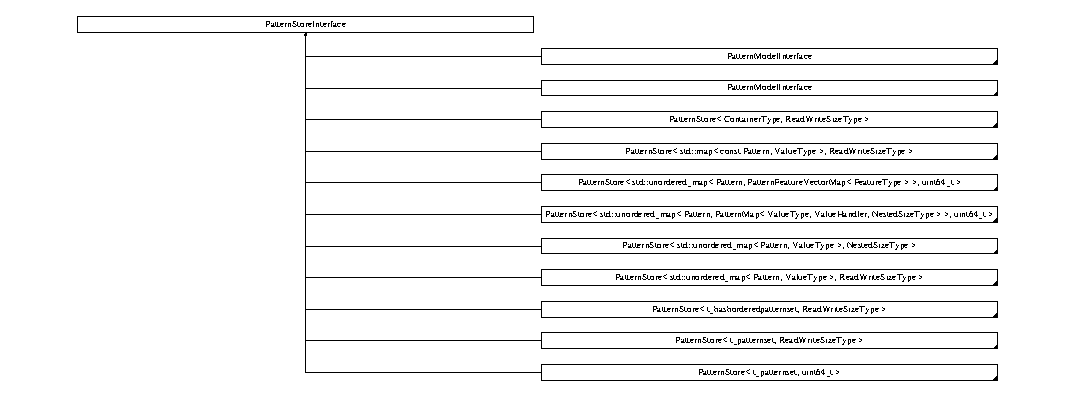
\includegraphics[height=5.318860cm]{classPatternStoreInterface}
\end{center}
\end{figure}
\subsection*{Public Member Functions}
\begin{DoxyCompactItemize}
\item 
virtual bool \hyperlink{classPatternStoreInterface_aec9f27496b38f8db1eced920fb2dc9fe}{has} (const \hyperlink{classPattern}{Pattern} \&) const  =0
\item 
virtual bool \hyperlink{classPatternStoreInterface_a6b3e80cd9021201ce8992ad6c293a354}{has} (const \hyperlink{classPatternPointer}{Pattern\+Pointer} \&) const  =0
\item 
virtual size\+\_\+t \hyperlink{classPatternStoreInterface_a225c319d318aad157512cd0001b05eb2}{size} () const  =0
\item 
virtual bool \hyperlink{classPatternStoreInterface_aec9f27496b38f8db1eced920fb2dc9fe}{has} (const \hyperlink{classPattern}{Pattern} \&) const  =0
\item 
virtual bool \hyperlink{classPatternStoreInterface_a6b3e80cd9021201ce8992ad6c293a354}{has} (const \hyperlink{classPatternPointer}{Pattern\+Pointer} \&) const  =0
\item 
virtual size\+\_\+t \hyperlink{classPatternStoreInterface_a225c319d318aad157512cd0001b05eb2}{size} () const  =0
\end{DoxyCompactItemize}


\subsection{Detailed Description}
Limited virtual interface to pattern stores. 

Limited interface to pattern stores 

\subsection{Member Function Documentation}
\hypertarget{classPatternStoreInterface_aec9f27496b38f8db1eced920fb2dc9fe}{}\index{Pattern\+Store\+Interface@{Pattern\+Store\+Interface}!has@{has}}
\index{has@{has}!Pattern\+Store\+Interface@{Pattern\+Store\+Interface}}
\subsubsection[{has(const Pattern \&) const  =0}]{\setlength{\rightskip}{0pt plus 5cm}virtual bool Pattern\+Store\+Interface\+::has (
\begin{DoxyParamCaption}
\item[{const {\bf Pattern} \&}]{}
\end{DoxyParamCaption}
) const\hspace{0.3cm}{\ttfamily [pure virtual]}}\label{classPatternStoreInterface_aec9f27496b38f8db1eced920fb2dc9fe}
Does the pattern occur in the pattern store? 

Implemented in \hyperlink{classHashOrderedPatternMap_a8682c2810f85d0c80ed015e388b571ef}{Hash\+Ordered\+Pattern\+Map$<$ Value\+Type, Value\+Handler, Read\+Write\+Size\+Type $>$}, \hyperlink{classOrderedPatternPointerMap_a646cdbf8491700740207b8fd980fbcc7}{Ordered\+Pattern\+Pointer\+Map$<$ Value\+Type, Value\+Handler, Read\+Write\+Size\+Type $>$}, \hyperlink{classPatternPointerMap_aff90e9b372ae3aed68cb037d91f65206}{Pattern\+Pointer\+Map$<$ Value\+Type, Value\+Handler, Read\+Write\+Size\+Type $>$}, \hyperlink{classPatternMap_a038d49e8aed58a207c3e106b086cdab0}{Pattern\+Map$<$ Value\+Type, Value\+Handler, Read\+Write\+Size\+Type $>$}, \hyperlink{classPatternMap_a038d49e8aed58a207c3e106b086cdab0}{Pattern\+Map$<$ Pattern\+Map$<$ Value\+Type, Value\+Handler, Nested\+Size\+Type $>$, Pattern\+Store\+Value\+Handler$<$ Pattern\+Map$<$ Value\+Type, Value\+Handler, Nested\+Size\+Type $>$ $>$, uint64\+\_\+t $>$}, \hyperlink{classPatternMap_a038d49e8aed58a207c3e106b086cdab0}{Pattern\+Map$<$ Value\+Type, Value\+Handler, Nested\+Size\+Type $>$}, \hyperlink{classPatternMap_a038d49e8aed58a207c3e106b086cdab0}{Pattern\+Map$<$ Pattern\+Feature\+Vector\+Map$<$ Feature\+Type $>$, Pattern\+Feature\+Vector\+Map\+Handler$<$ Feature\+Type $>$ $>$}, \hyperlink{classHashOrderedPatternSet_ac21ec186302af16a3b70c5c85e434510}{Hash\+Ordered\+Pattern\+Set$<$ Read\+Write\+Size\+Type $>$}, \hyperlink{classPatternModel_ad2fa89b6a2eb8d2aebb8553a9da42b84}{Pattern\+Model$<$ Value\+Type, Value\+Handler, Map\+Type, Pattern\+Type $>$}, \hyperlink{classPatternModel_ad2fa89b6a2eb8d2aebb8553a9da42b84}{Pattern\+Model$<$ Indexed\+Data, Indexed\+Data\+Handler, Map\+Type, Pattern\+Pointer $>$}, \hyperlink{classPatternModel_ad2fa89b6a2eb8d2aebb8553a9da42b84}{Pattern\+Model$<$ Indexed\+Data, Indexed\+Data\+Handler, Map\+Type, Pattern\+Type $>$}, \hyperlink{classPatternModel_ad2fa89b6a2eb8d2aebb8553a9da42b84}{Pattern\+Model$<$ Value\+Type, Value\+Handler, Map\+Type, Pattern\+Pointer $>$}, \hyperlink{classPatternSet_a25e9ec9ca33750f21dd729cd2462d925}{Pattern\+Set$<$ Read\+Write\+Size\+Type $>$}, \hyperlink{classPatternSet_a25e9ec9ca33750f21dd729cd2462d925}{Pattern\+Set$<$ uint64\+\_\+t $>$}, \hyperlink{classPatternMapStore_a208cf2d90725a3a9291d2dae67ac9256}{Pattern\+Map\+Store$<$ Container\+Type, Value\+Type, Value\+Handler, Read\+Write\+Size\+Type, Pattern\+Type $>$}, \hyperlink{classPatternMapStore_a208cf2d90725a3a9291d2dae67ac9256}{Pattern\+Map\+Store$<$ std\+::map$<$ Pattern\+Pointer, Value\+Type $>$, Value\+Type, Value\+Handler, Read\+Write\+Size\+Type, Pattern\+Pointer $>$}, \hyperlink{classPatternMapStore_a208cf2d90725a3a9291d2dae67ac9256}{Pattern\+Map\+Store$<$ std\+::unordered\+\_\+map$<$ Pattern, Value\+Type $>$, Value\+Type, Value\+Handler, Nested\+Size\+Type, Pattern $>$}, \hyperlink{classPatternMapStore_a208cf2d90725a3a9291d2dae67ac9256}{Pattern\+Map\+Store$<$ std\+::unordered\+\_\+map$<$ Pattern, Pattern\+Map$<$ Value\+Type, Value\+Handler, Nested\+Size\+Type $>$ $>$, Pattern\+Map$<$ Value\+Type, Value\+Handler, Nested\+Size\+Type $>$, Pattern\+Store\+Value\+Handler$<$ Pattern\+Map$<$ Value\+Type, Value\+Handler, Nested\+Size\+Type $>$ $>$, uint64\+\_\+t, Pattern $>$}, \hyperlink{classPatternMapStore_a208cf2d90725a3a9291d2dae67ac9256}{Pattern\+Map\+Store$<$ std\+::unordered\+\_\+map$<$ Pattern, Value\+Type $>$, Value\+Type, Value\+Handler, Read\+Write\+Size\+Type, Pattern $>$}, \hyperlink{classPatternMapStore_a208cf2d90725a3a9291d2dae67ac9256}{Pattern\+Map\+Store$<$ std\+::unordered\+\_\+map$<$ Pattern\+Pointer, Value\+Type $>$, Value\+Type, Value\+Handler, Read\+Write\+Size\+Type, Pattern\+Pointer $>$}, \hyperlink{classPatternMapStore_a208cf2d90725a3a9291d2dae67ac9256}{Pattern\+Map\+Store$<$ std\+::unordered\+\_\+map$<$ Pattern, Pattern\+Feature\+Vector\+Map$<$ Feature\+Type $>$ $>$, Pattern\+Feature\+Vector\+Map$<$ Feature\+Type $>$, Pattern\+Feature\+Vector\+Map\+Handler$<$ Feature\+Type $>$, uint64\+\_\+t, Pattern $>$}, \hyperlink{classPatternMapStore_a208cf2d90725a3a9291d2dae67ac9256}{Pattern\+Map\+Store$<$ std\+::map$<$ const Pattern, Value\+Type $>$, Value\+Type, Value\+Handler, Read\+Write\+Size\+Type, Pattern $>$}, \hyperlink{classPatternSetModel_a8821cf7c6d469d0978e32e5ed9cfcda0}{Pattern\+Set\+Model}, \hyperlink{classPatternStore_a2e29add9b35b3459d183f56f6c5525ed}{Pattern\+Store$<$ Container\+Type, Read\+Write\+Size\+Type, Pattern\+Type $>$}, \hyperlink{classPatternStore_a2e29add9b35b3459d183f56f6c5525ed}{Pattern\+Store$<$ std\+::map$<$ Pattern\+Pointer, Value\+Type $>$, Read\+Write\+Size\+Type, Pattern\+Pointer $>$}, \hyperlink{classPatternStore_a2e29add9b35b3459d183f56f6c5525ed}{Pattern\+Store$<$ std\+::unordered\+\_\+map$<$ Pattern\+Pointer, Value\+Type $>$, Read\+Write\+Size\+Type, Pattern\+Pointer $>$}, \hyperlink{classPatternStore_a2e29add9b35b3459d183f56f6c5525ed}{Pattern\+Store$<$ std\+::map$<$ const Pattern, Value\+Type $>$, Read\+Write\+Size\+Type, Pattern $>$}, \hyperlink{classPatternStore_a2e29add9b35b3459d183f56f6c5525ed}{Pattern\+Store$<$ std\+::unordered\+\_\+map$<$ Pattern, Value\+Type $>$, Read\+Write\+Size\+Type, Pattern $>$}, \hyperlink{classPatternStore_a2e29add9b35b3459d183f56f6c5525ed}{Pattern\+Store$<$ std\+::unordered\+\_\+map$<$ Pattern, Pattern\+Feature\+Vector\+Map$<$ Feature\+Type $>$ $>$, uint64\+\_\+t, Pattern $>$}, \hyperlink{classPatternStore_a2e29add9b35b3459d183f56f6c5525ed}{Pattern\+Store$<$ t\+\_\+patternset, uint64\+\_\+t, Pattern $>$}, \hyperlink{classPatternStore_a2e29add9b35b3459d183f56f6c5525ed}{Pattern\+Store$<$ t\+\_\+patternset, Read\+Write\+Size\+Type, Pattern $>$}, \hyperlink{classPatternStore_a2e29add9b35b3459d183f56f6c5525ed}{Pattern\+Store$<$ std\+::unordered\+\_\+map$<$ Pattern, Pattern\+Map$<$ Value\+Type, Value\+Handler, Nested\+Size\+Type $>$ $>$, uint64\+\_\+t, Pattern $>$}, \hyperlink{classPatternStore_a2e29add9b35b3459d183f56f6c5525ed}{Pattern\+Store$<$ t\+\_\+hashorderedpatternset, Read\+Write\+Size\+Type $>$}, \hyperlink{classPatternStore_a2e29add9b35b3459d183f56f6c5525ed}{Pattern\+Store$<$ std\+::unordered\+\_\+map$<$ Pattern, Value\+Type $>$, Nested\+Size\+Type, Pattern $>$}, and \hyperlink{classPatternAlignmentModel_a4822a730be0dabeebd06771c803b8254}{Pattern\+Alignment\+Model$<$ Feature\+Type $>$}.

\hypertarget{classPatternStoreInterface_a6b3e80cd9021201ce8992ad6c293a354}{}\index{Pattern\+Store\+Interface@{Pattern\+Store\+Interface}!has@{has}}
\index{has@{has}!Pattern\+Store\+Interface@{Pattern\+Store\+Interface}}
\subsubsection[{has(const Pattern\+Pointer \&) const  =0}]{\setlength{\rightskip}{0pt plus 5cm}virtual bool Pattern\+Store\+Interface\+::has (
\begin{DoxyParamCaption}
\item[{const {\bf Pattern\+Pointer} \&}]{}
\end{DoxyParamCaption}
) const\hspace{0.3cm}{\ttfamily [pure virtual]}}\label{classPatternStoreInterface_a6b3e80cd9021201ce8992ad6c293a354}
Does the pattern occur in the pattern store? 

Implemented in \hyperlink{classHashOrderedPatternMap_ae2b83d2bcc1378b817044c205bd60651}{Hash\+Ordered\+Pattern\+Map$<$ Value\+Type, Value\+Handler, Read\+Write\+Size\+Type $>$}, \hyperlink{classOrderedPatternPointerMap_a2bff7f96eb16357c7fb99049e2ad1223}{Ordered\+Pattern\+Pointer\+Map$<$ Value\+Type, Value\+Handler, Read\+Write\+Size\+Type $>$}, \hyperlink{classPatternPointerMap_ac8f06f6f2adcf655b0d46bcd999eeed9}{Pattern\+Pointer\+Map$<$ Value\+Type, Value\+Handler, Read\+Write\+Size\+Type $>$}, \hyperlink{classPatternMap_a18587e4b3c6143749b4b96e8f4808cdb}{Pattern\+Map$<$ Value\+Type, Value\+Handler, Read\+Write\+Size\+Type $>$}, \hyperlink{classPatternMap_a18587e4b3c6143749b4b96e8f4808cdb}{Pattern\+Map$<$ Pattern\+Map$<$ Value\+Type, Value\+Handler, Nested\+Size\+Type $>$, Pattern\+Store\+Value\+Handler$<$ Pattern\+Map$<$ Value\+Type, Value\+Handler, Nested\+Size\+Type $>$ $>$, uint64\+\_\+t $>$}, \hyperlink{classPatternMap_a18587e4b3c6143749b4b96e8f4808cdb}{Pattern\+Map$<$ Value\+Type, Value\+Handler, Nested\+Size\+Type $>$}, \hyperlink{classPatternMap_a18587e4b3c6143749b4b96e8f4808cdb}{Pattern\+Map$<$ Pattern\+Feature\+Vector\+Map$<$ Feature\+Type $>$, Pattern\+Feature\+Vector\+Map\+Handler$<$ Feature\+Type $>$ $>$}, \hyperlink{classHashOrderedPatternSet_a4d917cedc8386b463aae0ad86856c82a}{Hash\+Ordered\+Pattern\+Set$<$ Read\+Write\+Size\+Type $>$}, \hyperlink{classPatternModel_a3a5098f2c1606c0685ccf97ad9f6cad6}{Pattern\+Model$<$ Value\+Type, Value\+Handler, Map\+Type, Pattern\+Type $>$}, \hyperlink{classPatternModel_a3a5098f2c1606c0685ccf97ad9f6cad6}{Pattern\+Model$<$ Indexed\+Data, Indexed\+Data\+Handler, Map\+Type, Pattern\+Pointer $>$}, \hyperlink{classPatternModel_a3a5098f2c1606c0685ccf97ad9f6cad6}{Pattern\+Model$<$ Indexed\+Data, Indexed\+Data\+Handler, Map\+Type, Pattern\+Type $>$}, \hyperlink{classPatternModel_a3a5098f2c1606c0685ccf97ad9f6cad6}{Pattern\+Model$<$ Value\+Type, Value\+Handler, Map\+Type, Pattern\+Pointer $>$}, \hyperlink{classPatternSet_a28de1eeb8ec5774505173cc28e06320e}{Pattern\+Set$<$ Read\+Write\+Size\+Type $>$}, \hyperlink{classPatternSet_a28de1eeb8ec5774505173cc28e06320e}{Pattern\+Set$<$ uint64\+\_\+t $>$}, \hyperlink{classPatternMapStore_a4bce03112ff9c3c0950f31ccee0c9ab8}{Pattern\+Map\+Store$<$ Container\+Type, Value\+Type, Value\+Handler, Read\+Write\+Size\+Type, Pattern\+Type $>$}, \hyperlink{classPatternMapStore_a4bce03112ff9c3c0950f31ccee0c9ab8}{Pattern\+Map\+Store$<$ std\+::map$<$ Pattern\+Pointer, Value\+Type $>$, Value\+Type, Value\+Handler, Read\+Write\+Size\+Type, Pattern\+Pointer $>$}, \hyperlink{classPatternMapStore_a4bce03112ff9c3c0950f31ccee0c9ab8}{Pattern\+Map\+Store$<$ std\+::unordered\+\_\+map$<$ Pattern, Value\+Type $>$, Value\+Type, Value\+Handler, Nested\+Size\+Type, Pattern $>$}, \hyperlink{classPatternMapStore_a4bce03112ff9c3c0950f31ccee0c9ab8}{Pattern\+Map\+Store$<$ std\+::unordered\+\_\+map$<$ Pattern, Pattern\+Map$<$ Value\+Type, Value\+Handler, Nested\+Size\+Type $>$ $>$, Pattern\+Map$<$ Value\+Type, Value\+Handler, Nested\+Size\+Type $>$, Pattern\+Store\+Value\+Handler$<$ Pattern\+Map$<$ Value\+Type, Value\+Handler, Nested\+Size\+Type $>$ $>$, uint64\+\_\+t, Pattern $>$}, \hyperlink{classPatternMapStore_a4bce03112ff9c3c0950f31ccee0c9ab8}{Pattern\+Map\+Store$<$ std\+::unordered\+\_\+map$<$ Pattern, Value\+Type $>$, Value\+Type, Value\+Handler, Read\+Write\+Size\+Type, Pattern $>$}, \hyperlink{classPatternMapStore_a4bce03112ff9c3c0950f31ccee0c9ab8}{Pattern\+Map\+Store$<$ std\+::unordered\+\_\+map$<$ Pattern\+Pointer, Value\+Type $>$, Value\+Type, Value\+Handler, Read\+Write\+Size\+Type, Pattern\+Pointer $>$}, \hyperlink{classPatternMapStore_a4bce03112ff9c3c0950f31ccee0c9ab8}{Pattern\+Map\+Store$<$ std\+::unordered\+\_\+map$<$ Pattern, Pattern\+Feature\+Vector\+Map$<$ Feature\+Type $>$ $>$, Pattern\+Feature\+Vector\+Map$<$ Feature\+Type $>$, Pattern\+Feature\+Vector\+Map\+Handler$<$ Feature\+Type $>$, uint64\+\_\+t, Pattern $>$}, \hyperlink{classPatternMapStore_a4bce03112ff9c3c0950f31ccee0c9ab8}{Pattern\+Map\+Store$<$ std\+::map$<$ const Pattern, Value\+Type $>$, Value\+Type, Value\+Handler, Read\+Write\+Size\+Type, Pattern $>$}, \hyperlink{classPatternSetModel_a2fcd4d3d1023b5e20f67d2b845a29b2f}{Pattern\+Set\+Model}, \hyperlink{classPatternStore_ad1e06c2468bad2a14d4ed28b26c6ff33}{Pattern\+Store$<$ Container\+Type, Read\+Write\+Size\+Type, Pattern\+Type $>$}, \hyperlink{classPatternStore_ad1e06c2468bad2a14d4ed28b26c6ff33}{Pattern\+Store$<$ std\+::map$<$ Pattern\+Pointer, Value\+Type $>$, Read\+Write\+Size\+Type, Pattern\+Pointer $>$}, \hyperlink{classPatternStore_ad1e06c2468bad2a14d4ed28b26c6ff33}{Pattern\+Store$<$ std\+::unordered\+\_\+map$<$ Pattern\+Pointer, Value\+Type $>$, Read\+Write\+Size\+Type, Pattern\+Pointer $>$}, \hyperlink{classPatternStore_ad1e06c2468bad2a14d4ed28b26c6ff33}{Pattern\+Store$<$ std\+::map$<$ const Pattern, Value\+Type $>$, Read\+Write\+Size\+Type, Pattern $>$}, \hyperlink{classPatternStore_ad1e06c2468bad2a14d4ed28b26c6ff33}{Pattern\+Store$<$ std\+::unordered\+\_\+map$<$ Pattern, Value\+Type $>$, Read\+Write\+Size\+Type, Pattern $>$}, \hyperlink{classPatternStore_ad1e06c2468bad2a14d4ed28b26c6ff33}{Pattern\+Store$<$ std\+::unordered\+\_\+map$<$ Pattern, Pattern\+Feature\+Vector\+Map$<$ Feature\+Type $>$ $>$, uint64\+\_\+t, Pattern $>$}, \hyperlink{classPatternStore_ad1e06c2468bad2a14d4ed28b26c6ff33}{Pattern\+Store$<$ t\+\_\+patternset, uint64\+\_\+t, Pattern $>$}, \hyperlink{classPatternStore_ad1e06c2468bad2a14d4ed28b26c6ff33}{Pattern\+Store$<$ t\+\_\+patternset, Read\+Write\+Size\+Type, Pattern $>$}, \hyperlink{classPatternStore_ad1e06c2468bad2a14d4ed28b26c6ff33}{Pattern\+Store$<$ std\+::unordered\+\_\+map$<$ Pattern, Pattern\+Map$<$ Value\+Type, Value\+Handler, Nested\+Size\+Type $>$ $>$, uint64\+\_\+t, Pattern $>$}, \hyperlink{classPatternStore_ad1e06c2468bad2a14d4ed28b26c6ff33}{Pattern\+Store$<$ t\+\_\+hashorderedpatternset, Read\+Write\+Size\+Type $>$}, \hyperlink{classPatternStore_ad1e06c2468bad2a14d4ed28b26c6ff33}{Pattern\+Store$<$ std\+::unordered\+\_\+map$<$ Pattern, Value\+Type $>$, Nested\+Size\+Type, Pattern $>$}, and \hyperlink{classPatternAlignmentModel_ad81e599091c476a9cb121e7e04a4da5a}{Pattern\+Alignment\+Model$<$ Feature\+Type $>$}.

\hypertarget{classPatternStoreInterface_aec9f27496b38f8db1eced920fb2dc9fe}{}\index{Pattern\+Store\+Interface@{Pattern\+Store\+Interface}!has@{has}}
\index{has@{has}!Pattern\+Store\+Interface@{Pattern\+Store\+Interface}}
\subsubsection[{has(const Pattern \&) const  =0}]{\setlength{\rightskip}{0pt plus 5cm}virtual bool Pattern\+Store\+Interface\+::has (
\begin{DoxyParamCaption}
\item[{const {\bf Pattern} \&}]{}
\end{DoxyParamCaption}
) const\hspace{0.3cm}{\ttfamily [pure virtual]}}\label{classPatternStoreInterface_aec9f27496b38f8db1eced920fb2dc9fe}
Does the pattern occur in the pattern store? 

Implemented in \hyperlink{classHashOrderedPatternMap_a8682c2810f85d0c80ed015e388b571ef}{Hash\+Ordered\+Pattern\+Map$<$ Value\+Type, Value\+Handler, Read\+Write\+Size\+Type $>$}, \hyperlink{classOrderedPatternPointerMap_a646cdbf8491700740207b8fd980fbcc7}{Ordered\+Pattern\+Pointer\+Map$<$ Value\+Type, Value\+Handler, Read\+Write\+Size\+Type $>$}, \hyperlink{classPatternPointerMap_aff90e9b372ae3aed68cb037d91f65206}{Pattern\+Pointer\+Map$<$ Value\+Type, Value\+Handler, Read\+Write\+Size\+Type $>$}, \hyperlink{classPatternMap_a038d49e8aed58a207c3e106b086cdab0}{Pattern\+Map$<$ Value\+Type, Value\+Handler, Read\+Write\+Size\+Type $>$}, \hyperlink{classPatternMap_a038d49e8aed58a207c3e106b086cdab0}{Pattern\+Map$<$ Pattern\+Map$<$ Value\+Type, Value\+Handler, Nested\+Size\+Type $>$, Pattern\+Store\+Value\+Handler$<$ Pattern\+Map$<$ Value\+Type, Value\+Handler, Nested\+Size\+Type $>$ $>$, uint64\+\_\+t $>$}, \hyperlink{classPatternMap_a038d49e8aed58a207c3e106b086cdab0}{Pattern\+Map$<$ Value\+Type, Value\+Handler, Nested\+Size\+Type $>$}, \hyperlink{classPatternMap_a038d49e8aed58a207c3e106b086cdab0}{Pattern\+Map$<$ Pattern\+Feature\+Vector\+Map$<$ Feature\+Type $>$, Pattern\+Feature\+Vector\+Map\+Handler$<$ Feature\+Type $>$ $>$}, \hyperlink{classHashOrderedPatternSet_ac21ec186302af16a3b70c5c85e434510}{Hash\+Ordered\+Pattern\+Set$<$ Read\+Write\+Size\+Type $>$}, \hyperlink{classPatternModel_ad2fa89b6a2eb8d2aebb8553a9da42b84}{Pattern\+Model$<$ Value\+Type, Value\+Handler, Map\+Type, Pattern\+Type $>$}, \hyperlink{classPatternModel_ad2fa89b6a2eb8d2aebb8553a9da42b84}{Pattern\+Model$<$ Indexed\+Data, Indexed\+Data\+Handler, Map\+Type, Pattern\+Pointer $>$}, \hyperlink{classPatternModel_ad2fa89b6a2eb8d2aebb8553a9da42b84}{Pattern\+Model$<$ Indexed\+Data, Indexed\+Data\+Handler, Map\+Type, Pattern\+Type $>$}, \hyperlink{classPatternModel_ad2fa89b6a2eb8d2aebb8553a9da42b84}{Pattern\+Model$<$ Value\+Type, Value\+Handler, Map\+Type, Pattern\+Pointer $>$}, \hyperlink{classPatternSet_a25e9ec9ca33750f21dd729cd2462d925}{Pattern\+Set$<$ Read\+Write\+Size\+Type $>$}, \hyperlink{classPatternSet_a25e9ec9ca33750f21dd729cd2462d925}{Pattern\+Set$<$ uint64\+\_\+t $>$}, \hyperlink{classPatternMapStore_a208cf2d90725a3a9291d2dae67ac9256}{Pattern\+Map\+Store$<$ Container\+Type, Value\+Type, Value\+Handler, Read\+Write\+Size\+Type, Pattern\+Type $>$}, \hyperlink{classPatternMapStore_a208cf2d90725a3a9291d2dae67ac9256}{Pattern\+Map\+Store$<$ std\+::map$<$ Pattern\+Pointer, Value\+Type $>$, Value\+Type, Value\+Handler, Read\+Write\+Size\+Type, Pattern\+Pointer $>$}, \hyperlink{classPatternMapStore_a208cf2d90725a3a9291d2dae67ac9256}{Pattern\+Map\+Store$<$ std\+::unordered\+\_\+map$<$ Pattern, Value\+Type $>$, Value\+Type, Value\+Handler, Nested\+Size\+Type, Pattern $>$}, \hyperlink{classPatternMapStore_a208cf2d90725a3a9291d2dae67ac9256}{Pattern\+Map\+Store$<$ std\+::unordered\+\_\+map$<$ Pattern, Pattern\+Map$<$ Value\+Type, Value\+Handler, Nested\+Size\+Type $>$ $>$, Pattern\+Map$<$ Value\+Type, Value\+Handler, Nested\+Size\+Type $>$, Pattern\+Store\+Value\+Handler$<$ Pattern\+Map$<$ Value\+Type, Value\+Handler, Nested\+Size\+Type $>$ $>$, uint64\+\_\+t, Pattern $>$}, \hyperlink{classPatternMapStore_a208cf2d90725a3a9291d2dae67ac9256}{Pattern\+Map\+Store$<$ std\+::unordered\+\_\+map$<$ Pattern, Value\+Type $>$, Value\+Type, Value\+Handler, Read\+Write\+Size\+Type, Pattern $>$}, \hyperlink{classPatternMapStore_a208cf2d90725a3a9291d2dae67ac9256}{Pattern\+Map\+Store$<$ std\+::unordered\+\_\+map$<$ Pattern\+Pointer, Value\+Type $>$, Value\+Type, Value\+Handler, Read\+Write\+Size\+Type, Pattern\+Pointer $>$}, \hyperlink{classPatternMapStore_a208cf2d90725a3a9291d2dae67ac9256}{Pattern\+Map\+Store$<$ std\+::unordered\+\_\+map$<$ Pattern, Pattern\+Feature\+Vector\+Map$<$ Feature\+Type $>$ $>$, Pattern\+Feature\+Vector\+Map$<$ Feature\+Type $>$, Pattern\+Feature\+Vector\+Map\+Handler$<$ Feature\+Type $>$, uint64\+\_\+t, Pattern $>$}, \hyperlink{classPatternMapStore_a208cf2d90725a3a9291d2dae67ac9256}{Pattern\+Map\+Store$<$ std\+::map$<$ const Pattern, Value\+Type $>$, Value\+Type, Value\+Handler, Read\+Write\+Size\+Type, Pattern $>$}, \hyperlink{classPatternSetModel_a8821cf7c6d469d0978e32e5ed9cfcda0}{Pattern\+Set\+Model}, \hyperlink{classPatternStore_a2e29add9b35b3459d183f56f6c5525ed}{Pattern\+Store$<$ Container\+Type, Read\+Write\+Size\+Type, Pattern\+Type $>$}, \hyperlink{classPatternStore_a2e29add9b35b3459d183f56f6c5525ed}{Pattern\+Store$<$ std\+::map$<$ Pattern\+Pointer, Value\+Type $>$, Read\+Write\+Size\+Type, Pattern\+Pointer $>$}, \hyperlink{classPatternStore_a2e29add9b35b3459d183f56f6c5525ed}{Pattern\+Store$<$ std\+::unordered\+\_\+map$<$ Pattern\+Pointer, Value\+Type $>$, Read\+Write\+Size\+Type, Pattern\+Pointer $>$}, \hyperlink{classPatternStore_a2e29add9b35b3459d183f56f6c5525ed}{Pattern\+Store$<$ std\+::map$<$ const Pattern, Value\+Type $>$, Read\+Write\+Size\+Type, Pattern $>$}, \hyperlink{classPatternStore_a2e29add9b35b3459d183f56f6c5525ed}{Pattern\+Store$<$ std\+::unordered\+\_\+map$<$ Pattern, Value\+Type $>$, Read\+Write\+Size\+Type, Pattern $>$}, \hyperlink{classPatternStore_a2e29add9b35b3459d183f56f6c5525ed}{Pattern\+Store$<$ std\+::unordered\+\_\+map$<$ Pattern, Pattern\+Feature\+Vector\+Map$<$ Feature\+Type $>$ $>$, uint64\+\_\+t, Pattern $>$}, \hyperlink{classPatternStore_a2e29add9b35b3459d183f56f6c5525ed}{Pattern\+Store$<$ t\+\_\+patternset, uint64\+\_\+t, Pattern $>$}, \hyperlink{classPatternStore_a2e29add9b35b3459d183f56f6c5525ed}{Pattern\+Store$<$ t\+\_\+patternset, Read\+Write\+Size\+Type, Pattern $>$}, \hyperlink{classPatternStore_a2e29add9b35b3459d183f56f6c5525ed}{Pattern\+Store$<$ std\+::unordered\+\_\+map$<$ Pattern, Pattern\+Map$<$ Value\+Type, Value\+Handler, Nested\+Size\+Type $>$ $>$, uint64\+\_\+t, Pattern $>$}, \hyperlink{classPatternStore_a2e29add9b35b3459d183f56f6c5525ed}{Pattern\+Store$<$ t\+\_\+hashorderedpatternset, Read\+Write\+Size\+Type $>$}, \hyperlink{classPatternStore_a2e29add9b35b3459d183f56f6c5525ed}{Pattern\+Store$<$ std\+::unordered\+\_\+map$<$ Pattern, Value\+Type $>$, Nested\+Size\+Type, Pattern $>$}, and \hyperlink{classPatternAlignmentModel_a4822a730be0dabeebd06771c803b8254}{Pattern\+Alignment\+Model$<$ Feature\+Type $>$}.

\hypertarget{classPatternStoreInterface_a6b3e80cd9021201ce8992ad6c293a354}{}\index{Pattern\+Store\+Interface@{Pattern\+Store\+Interface}!has@{has}}
\index{has@{has}!Pattern\+Store\+Interface@{Pattern\+Store\+Interface}}
\subsubsection[{has(const Pattern\+Pointer \&) const  =0}]{\setlength{\rightskip}{0pt plus 5cm}virtual bool Pattern\+Store\+Interface\+::has (
\begin{DoxyParamCaption}
\item[{const {\bf Pattern\+Pointer} \&}]{}
\end{DoxyParamCaption}
) const\hspace{0.3cm}{\ttfamily [pure virtual]}}\label{classPatternStoreInterface_a6b3e80cd9021201ce8992ad6c293a354}
Does the pattern occur in the pattern store? 

Implemented in \hyperlink{classHashOrderedPatternMap_ae2b83d2bcc1378b817044c205bd60651}{Hash\+Ordered\+Pattern\+Map$<$ Value\+Type, Value\+Handler, Read\+Write\+Size\+Type $>$}, \hyperlink{classOrderedPatternPointerMap_a2bff7f96eb16357c7fb99049e2ad1223}{Ordered\+Pattern\+Pointer\+Map$<$ Value\+Type, Value\+Handler, Read\+Write\+Size\+Type $>$}, \hyperlink{classPatternPointerMap_ac8f06f6f2adcf655b0d46bcd999eeed9}{Pattern\+Pointer\+Map$<$ Value\+Type, Value\+Handler, Read\+Write\+Size\+Type $>$}, \hyperlink{classPatternMap_a18587e4b3c6143749b4b96e8f4808cdb}{Pattern\+Map$<$ Value\+Type, Value\+Handler, Read\+Write\+Size\+Type $>$}, \hyperlink{classPatternMap_a18587e4b3c6143749b4b96e8f4808cdb}{Pattern\+Map$<$ Pattern\+Map$<$ Value\+Type, Value\+Handler, Nested\+Size\+Type $>$, Pattern\+Store\+Value\+Handler$<$ Pattern\+Map$<$ Value\+Type, Value\+Handler, Nested\+Size\+Type $>$ $>$, uint64\+\_\+t $>$}, \hyperlink{classPatternMap_a18587e4b3c6143749b4b96e8f4808cdb}{Pattern\+Map$<$ Value\+Type, Value\+Handler, Nested\+Size\+Type $>$}, \hyperlink{classPatternMap_a18587e4b3c6143749b4b96e8f4808cdb}{Pattern\+Map$<$ Pattern\+Feature\+Vector\+Map$<$ Feature\+Type $>$, Pattern\+Feature\+Vector\+Map\+Handler$<$ Feature\+Type $>$ $>$}, \hyperlink{classHashOrderedPatternSet_a4d917cedc8386b463aae0ad86856c82a}{Hash\+Ordered\+Pattern\+Set$<$ Read\+Write\+Size\+Type $>$}, \hyperlink{classPatternModel_a3a5098f2c1606c0685ccf97ad9f6cad6}{Pattern\+Model$<$ Value\+Type, Value\+Handler, Map\+Type, Pattern\+Type $>$}, \hyperlink{classPatternModel_a3a5098f2c1606c0685ccf97ad9f6cad6}{Pattern\+Model$<$ Indexed\+Data, Indexed\+Data\+Handler, Map\+Type, Pattern\+Pointer $>$}, \hyperlink{classPatternModel_a3a5098f2c1606c0685ccf97ad9f6cad6}{Pattern\+Model$<$ Indexed\+Data, Indexed\+Data\+Handler, Map\+Type, Pattern\+Type $>$}, \hyperlink{classPatternModel_a3a5098f2c1606c0685ccf97ad9f6cad6}{Pattern\+Model$<$ Value\+Type, Value\+Handler, Map\+Type, Pattern\+Pointer $>$}, \hyperlink{classPatternSet_a28de1eeb8ec5774505173cc28e06320e}{Pattern\+Set$<$ Read\+Write\+Size\+Type $>$}, \hyperlink{classPatternSet_a28de1eeb8ec5774505173cc28e06320e}{Pattern\+Set$<$ uint64\+\_\+t $>$}, \hyperlink{classPatternMapStore_a4bce03112ff9c3c0950f31ccee0c9ab8}{Pattern\+Map\+Store$<$ Container\+Type, Value\+Type, Value\+Handler, Read\+Write\+Size\+Type, Pattern\+Type $>$}, \hyperlink{classPatternMapStore_a4bce03112ff9c3c0950f31ccee0c9ab8}{Pattern\+Map\+Store$<$ std\+::map$<$ Pattern\+Pointer, Value\+Type $>$, Value\+Type, Value\+Handler, Read\+Write\+Size\+Type, Pattern\+Pointer $>$}, \hyperlink{classPatternMapStore_a4bce03112ff9c3c0950f31ccee0c9ab8}{Pattern\+Map\+Store$<$ std\+::unordered\+\_\+map$<$ Pattern, Value\+Type $>$, Value\+Type, Value\+Handler, Nested\+Size\+Type, Pattern $>$}, \hyperlink{classPatternMapStore_a4bce03112ff9c3c0950f31ccee0c9ab8}{Pattern\+Map\+Store$<$ std\+::unordered\+\_\+map$<$ Pattern, Pattern\+Map$<$ Value\+Type, Value\+Handler, Nested\+Size\+Type $>$ $>$, Pattern\+Map$<$ Value\+Type, Value\+Handler, Nested\+Size\+Type $>$, Pattern\+Store\+Value\+Handler$<$ Pattern\+Map$<$ Value\+Type, Value\+Handler, Nested\+Size\+Type $>$ $>$, uint64\+\_\+t, Pattern $>$}, \hyperlink{classPatternMapStore_a4bce03112ff9c3c0950f31ccee0c9ab8}{Pattern\+Map\+Store$<$ std\+::unordered\+\_\+map$<$ Pattern, Value\+Type $>$, Value\+Type, Value\+Handler, Read\+Write\+Size\+Type, Pattern $>$}, \hyperlink{classPatternMapStore_a4bce03112ff9c3c0950f31ccee0c9ab8}{Pattern\+Map\+Store$<$ std\+::unordered\+\_\+map$<$ Pattern\+Pointer, Value\+Type $>$, Value\+Type, Value\+Handler, Read\+Write\+Size\+Type, Pattern\+Pointer $>$}, \hyperlink{classPatternMapStore_a4bce03112ff9c3c0950f31ccee0c9ab8}{Pattern\+Map\+Store$<$ std\+::unordered\+\_\+map$<$ Pattern, Pattern\+Feature\+Vector\+Map$<$ Feature\+Type $>$ $>$, Pattern\+Feature\+Vector\+Map$<$ Feature\+Type $>$, Pattern\+Feature\+Vector\+Map\+Handler$<$ Feature\+Type $>$, uint64\+\_\+t, Pattern $>$}, \hyperlink{classPatternMapStore_a4bce03112ff9c3c0950f31ccee0c9ab8}{Pattern\+Map\+Store$<$ std\+::map$<$ const Pattern, Value\+Type $>$, Value\+Type, Value\+Handler, Read\+Write\+Size\+Type, Pattern $>$}, \hyperlink{classPatternSetModel_a2fcd4d3d1023b5e20f67d2b845a29b2f}{Pattern\+Set\+Model}, \hyperlink{classPatternStore_ad1e06c2468bad2a14d4ed28b26c6ff33}{Pattern\+Store$<$ Container\+Type, Read\+Write\+Size\+Type, Pattern\+Type $>$}, \hyperlink{classPatternStore_ad1e06c2468bad2a14d4ed28b26c6ff33}{Pattern\+Store$<$ std\+::map$<$ Pattern\+Pointer, Value\+Type $>$, Read\+Write\+Size\+Type, Pattern\+Pointer $>$}, \hyperlink{classPatternStore_ad1e06c2468bad2a14d4ed28b26c6ff33}{Pattern\+Store$<$ std\+::unordered\+\_\+map$<$ Pattern\+Pointer, Value\+Type $>$, Read\+Write\+Size\+Type, Pattern\+Pointer $>$}, \hyperlink{classPatternStore_ad1e06c2468bad2a14d4ed28b26c6ff33}{Pattern\+Store$<$ std\+::map$<$ const Pattern, Value\+Type $>$, Read\+Write\+Size\+Type, Pattern $>$}, \hyperlink{classPatternStore_ad1e06c2468bad2a14d4ed28b26c6ff33}{Pattern\+Store$<$ std\+::unordered\+\_\+map$<$ Pattern, Value\+Type $>$, Read\+Write\+Size\+Type, Pattern $>$}, \hyperlink{classPatternStore_ad1e06c2468bad2a14d4ed28b26c6ff33}{Pattern\+Store$<$ std\+::unordered\+\_\+map$<$ Pattern, Pattern\+Feature\+Vector\+Map$<$ Feature\+Type $>$ $>$, uint64\+\_\+t, Pattern $>$}, \hyperlink{classPatternStore_ad1e06c2468bad2a14d4ed28b26c6ff33}{Pattern\+Store$<$ t\+\_\+patternset, uint64\+\_\+t, Pattern $>$}, \hyperlink{classPatternStore_ad1e06c2468bad2a14d4ed28b26c6ff33}{Pattern\+Store$<$ t\+\_\+patternset, Read\+Write\+Size\+Type, Pattern $>$}, \hyperlink{classPatternStore_ad1e06c2468bad2a14d4ed28b26c6ff33}{Pattern\+Store$<$ std\+::unordered\+\_\+map$<$ Pattern, Pattern\+Map$<$ Value\+Type, Value\+Handler, Nested\+Size\+Type $>$ $>$, uint64\+\_\+t, Pattern $>$}, \hyperlink{classPatternStore_ad1e06c2468bad2a14d4ed28b26c6ff33}{Pattern\+Store$<$ t\+\_\+hashorderedpatternset, Read\+Write\+Size\+Type $>$}, \hyperlink{classPatternStore_ad1e06c2468bad2a14d4ed28b26c6ff33}{Pattern\+Store$<$ std\+::unordered\+\_\+map$<$ Pattern, Value\+Type $>$, Nested\+Size\+Type, Pattern $>$}, and \hyperlink{classPatternAlignmentModel_ad81e599091c476a9cb121e7e04a4da5a}{Pattern\+Alignment\+Model$<$ Feature\+Type $>$}.

\hypertarget{classPatternStoreInterface_a225c319d318aad157512cd0001b05eb2}{}\index{Pattern\+Store\+Interface@{Pattern\+Store\+Interface}!size@{size}}
\index{size@{size}!Pattern\+Store\+Interface@{Pattern\+Store\+Interface}}
\subsubsection[{size() const  =0}]{\setlength{\rightskip}{0pt plus 5cm}virtual size\+\_\+t Pattern\+Store\+Interface\+::size (
\begin{DoxyParamCaption}
{}
\end{DoxyParamCaption}
) const\hspace{0.3cm}{\ttfamily [pure virtual]}}\label{classPatternStoreInterface_a225c319d318aad157512cd0001b05eb2}
How many patterns are in the pattern store? 

Implemented in \hyperlink{classHashOrderedPatternMap_a5a48798964b7d667950f41630d3bf708}{Hash\+Ordered\+Pattern\+Map$<$ Value\+Type, Value\+Handler, Read\+Write\+Size\+Type $>$}, \hyperlink{classOrderedPatternPointerMap_a58dd12c7a840c59ec9d90461c7e5e8ce}{Ordered\+Pattern\+Pointer\+Map$<$ Value\+Type, Value\+Handler, Read\+Write\+Size\+Type $>$}, \hyperlink{classPatternPointerMap_a84be24690f7548478cdb123479729aa5}{Pattern\+Pointer\+Map$<$ Value\+Type, Value\+Handler, Read\+Write\+Size\+Type $>$}, \hyperlink{classPatternMap_aed30070f31256d0c1335fa9bd3b5db1c}{Pattern\+Map$<$ Value\+Type, Value\+Handler, Read\+Write\+Size\+Type $>$}, \hyperlink{classPatternMap_aed30070f31256d0c1335fa9bd3b5db1c}{Pattern\+Map$<$ Pattern\+Map$<$ Value\+Type, Value\+Handler, Nested\+Size\+Type $>$, Pattern\+Store\+Value\+Handler$<$ Pattern\+Map$<$ Value\+Type, Value\+Handler, Nested\+Size\+Type $>$ $>$, uint64\+\_\+t $>$}, \hyperlink{classPatternMap_aed30070f31256d0c1335fa9bd3b5db1c}{Pattern\+Map$<$ Value\+Type, Value\+Handler, Nested\+Size\+Type $>$}, \hyperlink{classPatternMap_aed30070f31256d0c1335fa9bd3b5db1c}{Pattern\+Map$<$ Pattern\+Feature\+Vector\+Map$<$ Feature\+Type $>$, Pattern\+Feature\+Vector\+Map\+Handler$<$ Feature\+Type $>$ $>$}, \hyperlink{classHashOrderedPatternSet_a42fee5ee6f163edf807623ffc6ab2617}{Hash\+Ordered\+Pattern\+Set$<$ Read\+Write\+Size\+Type $>$}, \hyperlink{classPatternModel_a2422cb944da209f399b3b10f3b1d2684}{Pattern\+Model$<$ Value\+Type, Value\+Handler, Map\+Type, Pattern\+Type $>$}, \hyperlink{classPatternModel_a2422cb944da209f399b3b10f3b1d2684}{Pattern\+Model$<$ Indexed\+Data, Indexed\+Data\+Handler, Map\+Type, Pattern\+Pointer $>$}, \hyperlink{classPatternModel_a2422cb944da209f399b3b10f3b1d2684}{Pattern\+Model$<$ Indexed\+Data, Indexed\+Data\+Handler, Map\+Type, Pattern\+Type $>$}, \hyperlink{classPatternModel_a2422cb944da209f399b3b10f3b1d2684}{Pattern\+Model$<$ Value\+Type, Value\+Handler, Map\+Type, Pattern\+Pointer $>$}, \hyperlink{classPatternSet_af85860d7135a5154a01a8366131beb39}{Pattern\+Set$<$ Read\+Write\+Size\+Type $>$}, \hyperlink{classPatternSet_af85860d7135a5154a01a8366131beb39}{Pattern\+Set$<$ uint64\+\_\+t $>$}, \hyperlink{classPatternMapStore_af7bd333e776a4e55af9add5ee320dbb5}{Pattern\+Map\+Store$<$ Container\+Type, Value\+Type, Value\+Handler, Read\+Write\+Size\+Type, Pattern\+Type $>$}, \hyperlink{classPatternMapStore_af7bd333e776a4e55af9add5ee320dbb5}{Pattern\+Map\+Store$<$ std\+::map$<$ Pattern\+Pointer, Value\+Type $>$, Value\+Type, Value\+Handler, Read\+Write\+Size\+Type, Pattern\+Pointer $>$}, \hyperlink{classPatternMapStore_af7bd333e776a4e55af9add5ee320dbb5}{Pattern\+Map\+Store$<$ std\+::unordered\+\_\+map$<$ Pattern, Value\+Type $>$, Value\+Type, Value\+Handler, Nested\+Size\+Type, Pattern $>$}, \hyperlink{classPatternMapStore_af7bd333e776a4e55af9add5ee320dbb5}{Pattern\+Map\+Store$<$ std\+::unordered\+\_\+map$<$ Pattern, Pattern\+Map$<$ Value\+Type, Value\+Handler, Nested\+Size\+Type $>$ $>$, Pattern\+Map$<$ Value\+Type, Value\+Handler, Nested\+Size\+Type $>$, Pattern\+Store\+Value\+Handler$<$ Pattern\+Map$<$ Value\+Type, Value\+Handler, Nested\+Size\+Type $>$ $>$, uint64\+\_\+t, Pattern $>$}, \hyperlink{classPatternMapStore_af7bd333e776a4e55af9add5ee320dbb5}{Pattern\+Map\+Store$<$ std\+::unordered\+\_\+map$<$ Pattern, Value\+Type $>$, Value\+Type, Value\+Handler, Read\+Write\+Size\+Type, Pattern $>$}, \hyperlink{classPatternMapStore_af7bd333e776a4e55af9add5ee320dbb5}{Pattern\+Map\+Store$<$ std\+::unordered\+\_\+map$<$ Pattern\+Pointer, Value\+Type $>$, Value\+Type, Value\+Handler, Read\+Write\+Size\+Type, Pattern\+Pointer $>$}, \hyperlink{classPatternMapStore_af7bd333e776a4e55af9add5ee320dbb5}{Pattern\+Map\+Store$<$ std\+::unordered\+\_\+map$<$ Pattern, Pattern\+Feature\+Vector\+Map$<$ Feature\+Type $>$ $>$, Pattern\+Feature\+Vector\+Map$<$ Feature\+Type $>$, Pattern\+Feature\+Vector\+Map\+Handler$<$ Feature\+Type $>$, uint64\+\_\+t, Pattern $>$}, \hyperlink{classPatternMapStore_af7bd333e776a4e55af9add5ee320dbb5}{Pattern\+Map\+Store$<$ std\+::map$<$ const Pattern, Value\+Type $>$, Value\+Type, Value\+Handler, Read\+Write\+Size\+Type, Pattern $>$}, \hyperlink{classPatternStore_abfa82df94ab565bea13fc45ee4866faf}{Pattern\+Store$<$ Container\+Type, Read\+Write\+Size\+Type, Pattern\+Type $>$}, \hyperlink{classPatternStore_abfa82df94ab565bea13fc45ee4866faf}{Pattern\+Store$<$ std\+::map$<$ Pattern\+Pointer, Value\+Type $>$, Read\+Write\+Size\+Type, Pattern\+Pointer $>$}, \hyperlink{classPatternStore_abfa82df94ab565bea13fc45ee4866faf}{Pattern\+Store$<$ std\+::unordered\+\_\+map$<$ Pattern\+Pointer, Value\+Type $>$, Read\+Write\+Size\+Type, Pattern\+Pointer $>$}, \hyperlink{classPatternStore_abfa82df94ab565bea13fc45ee4866faf}{Pattern\+Store$<$ std\+::map$<$ const Pattern, Value\+Type $>$, Read\+Write\+Size\+Type, Pattern $>$}, \hyperlink{classPatternStore_abfa82df94ab565bea13fc45ee4866faf}{Pattern\+Store$<$ std\+::unordered\+\_\+map$<$ Pattern, Value\+Type $>$, Read\+Write\+Size\+Type, Pattern $>$}, \hyperlink{classPatternStore_abfa82df94ab565bea13fc45ee4866faf}{Pattern\+Store$<$ std\+::unordered\+\_\+map$<$ Pattern, Pattern\+Feature\+Vector\+Map$<$ Feature\+Type $>$ $>$, uint64\+\_\+t, Pattern $>$}, \hyperlink{classPatternStore_abfa82df94ab565bea13fc45ee4866faf}{Pattern\+Store$<$ t\+\_\+patternset, uint64\+\_\+t, Pattern $>$}, \hyperlink{classPatternStore_abfa82df94ab565bea13fc45ee4866faf}{Pattern\+Store$<$ t\+\_\+patternset, Read\+Write\+Size\+Type, Pattern $>$}, \hyperlink{classPatternStore_abfa82df94ab565bea13fc45ee4866faf}{Pattern\+Store$<$ std\+::unordered\+\_\+map$<$ Pattern, Pattern\+Map$<$ Value\+Type, Value\+Handler, Nested\+Size\+Type $>$ $>$, uint64\+\_\+t, Pattern $>$}, \hyperlink{classPatternStore_abfa82df94ab565bea13fc45ee4866faf}{Pattern\+Store$<$ t\+\_\+hashorderedpatternset, Read\+Write\+Size\+Type $>$}, \hyperlink{classPatternStore_abfa82df94ab565bea13fc45ee4866faf}{Pattern\+Store$<$ std\+::unordered\+\_\+map$<$ Pattern, Value\+Type $>$, Nested\+Size\+Type, Pattern $>$}, \hyperlink{classPatternSetModel_aa19ae308dbc4bf1db35be6ba7ff4769b}{Pattern\+Set\+Model}, and \hyperlink{classPatternAlignmentModel_a7e4b2a69fd2e0852af0ed6ffaf6c51dc}{Pattern\+Alignment\+Model$<$ Feature\+Type $>$}.

\hypertarget{classPatternStoreInterface_a225c319d318aad157512cd0001b05eb2}{}\index{Pattern\+Store\+Interface@{Pattern\+Store\+Interface}!size@{size}}
\index{size@{size}!Pattern\+Store\+Interface@{Pattern\+Store\+Interface}}
\subsubsection[{size() const  =0}]{\setlength{\rightskip}{0pt plus 5cm}virtual size\+\_\+t Pattern\+Store\+Interface\+::size (
\begin{DoxyParamCaption}
{}
\end{DoxyParamCaption}
) const\hspace{0.3cm}{\ttfamily [pure virtual]}}\label{classPatternStoreInterface_a225c319d318aad157512cd0001b05eb2}
How many patterns are in the pattern store? 

Implemented in \hyperlink{classHashOrderedPatternMap_a5a48798964b7d667950f41630d3bf708}{Hash\+Ordered\+Pattern\+Map$<$ Value\+Type, Value\+Handler, Read\+Write\+Size\+Type $>$}, \hyperlink{classOrderedPatternPointerMap_a58dd12c7a840c59ec9d90461c7e5e8ce}{Ordered\+Pattern\+Pointer\+Map$<$ Value\+Type, Value\+Handler, Read\+Write\+Size\+Type $>$}, \hyperlink{classPatternPointerMap_a84be24690f7548478cdb123479729aa5}{Pattern\+Pointer\+Map$<$ Value\+Type, Value\+Handler, Read\+Write\+Size\+Type $>$}, \hyperlink{classPatternMap_aed30070f31256d0c1335fa9bd3b5db1c}{Pattern\+Map$<$ Value\+Type, Value\+Handler, Read\+Write\+Size\+Type $>$}, \hyperlink{classPatternMap_aed30070f31256d0c1335fa9bd3b5db1c}{Pattern\+Map$<$ Pattern\+Map$<$ Value\+Type, Value\+Handler, Nested\+Size\+Type $>$, Pattern\+Store\+Value\+Handler$<$ Pattern\+Map$<$ Value\+Type, Value\+Handler, Nested\+Size\+Type $>$ $>$, uint64\+\_\+t $>$}, \hyperlink{classPatternMap_aed30070f31256d0c1335fa9bd3b5db1c}{Pattern\+Map$<$ Value\+Type, Value\+Handler, Nested\+Size\+Type $>$}, \hyperlink{classPatternMap_aed30070f31256d0c1335fa9bd3b5db1c}{Pattern\+Map$<$ Pattern\+Feature\+Vector\+Map$<$ Feature\+Type $>$, Pattern\+Feature\+Vector\+Map\+Handler$<$ Feature\+Type $>$ $>$}, \hyperlink{classHashOrderedPatternSet_a42fee5ee6f163edf807623ffc6ab2617}{Hash\+Ordered\+Pattern\+Set$<$ Read\+Write\+Size\+Type $>$}, \hyperlink{classPatternModel_a2422cb944da209f399b3b10f3b1d2684}{Pattern\+Model$<$ Value\+Type, Value\+Handler, Map\+Type, Pattern\+Type $>$}, \hyperlink{classPatternModel_a2422cb944da209f399b3b10f3b1d2684}{Pattern\+Model$<$ Indexed\+Data, Indexed\+Data\+Handler, Map\+Type, Pattern\+Pointer $>$}, \hyperlink{classPatternModel_a2422cb944da209f399b3b10f3b1d2684}{Pattern\+Model$<$ Indexed\+Data, Indexed\+Data\+Handler, Map\+Type, Pattern\+Type $>$}, \hyperlink{classPatternModel_a2422cb944da209f399b3b10f3b1d2684}{Pattern\+Model$<$ Value\+Type, Value\+Handler, Map\+Type, Pattern\+Pointer $>$}, \hyperlink{classPatternSet_af85860d7135a5154a01a8366131beb39}{Pattern\+Set$<$ Read\+Write\+Size\+Type $>$}, \hyperlink{classPatternSet_af85860d7135a5154a01a8366131beb39}{Pattern\+Set$<$ uint64\+\_\+t $>$}, \hyperlink{classPatternMapStore_af7bd333e776a4e55af9add5ee320dbb5}{Pattern\+Map\+Store$<$ Container\+Type, Value\+Type, Value\+Handler, Read\+Write\+Size\+Type, Pattern\+Type $>$}, \hyperlink{classPatternMapStore_af7bd333e776a4e55af9add5ee320dbb5}{Pattern\+Map\+Store$<$ std\+::map$<$ Pattern\+Pointer, Value\+Type $>$, Value\+Type, Value\+Handler, Read\+Write\+Size\+Type, Pattern\+Pointer $>$}, \hyperlink{classPatternMapStore_af7bd333e776a4e55af9add5ee320dbb5}{Pattern\+Map\+Store$<$ std\+::unordered\+\_\+map$<$ Pattern, Value\+Type $>$, Value\+Type, Value\+Handler, Nested\+Size\+Type, Pattern $>$}, \hyperlink{classPatternMapStore_af7bd333e776a4e55af9add5ee320dbb5}{Pattern\+Map\+Store$<$ std\+::unordered\+\_\+map$<$ Pattern, Pattern\+Map$<$ Value\+Type, Value\+Handler, Nested\+Size\+Type $>$ $>$, Pattern\+Map$<$ Value\+Type, Value\+Handler, Nested\+Size\+Type $>$, Pattern\+Store\+Value\+Handler$<$ Pattern\+Map$<$ Value\+Type, Value\+Handler, Nested\+Size\+Type $>$ $>$, uint64\+\_\+t, Pattern $>$}, \hyperlink{classPatternMapStore_af7bd333e776a4e55af9add5ee320dbb5}{Pattern\+Map\+Store$<$ std\+::unordered\+\_\+map$<$ Pattern, Value\+Type $>$, Value\+Type, Value\+Handler, Read\+Write\+Size\+Type, Pattern $>$}, \hyperlink{classPatternMapStore_af7bd333e776a4e55af9add5ee320dbb5}{Pattern\+Map\+Store$<$ std\+::unordered\+\_\+map$<$ Pattern\+Pointer, Value\+Type $>$, Value\+Type, Value\+Handler, Read\+Write\+Size\+Type, Pattern\+Pointer $>$}, \hyperlink{classPatternMapStore_af7bd333e776a4e55af9add5ee320dbb5}{Pattern\+Map\+Store$<$ std\+::unordered\+\_\+map$<$ Pattern, Pattern\+Feature\+Vector\+Map$<$ Feature\+Type $>$ $>$, Pattern\+Feature\+Vector\+Map$<$ Feature\+Type $>$, Pattern\+Feature\+Vector\+Map\+Handler$<$ Feature\+Type $>$, uint64\+\_\+t, Pattern $>$}, \hyperlink{classPatternMapStore_af7bd333e776a4e55af9add5ee320dbb5}{Pattern\+Map\+Store$<$ std\+::map$<$ const Pattern, Value\+Type $>$, Value\+Type, Value\+Handler, Read\+Write\+Size\+Type, Pattern $>$}, \hyperlink{classPatternStore_abfa82df94ab565bea13fc45ee4866faf}{Pattern\+Store$<$ Container\+Type, Read\+Write\+Size\+Type, Pattern\+Type $>$}, \hyperlink{classPatternStore_abfa82df94ab565bea13fc45ee4866faf}{Pattern\+Store$<$ std\+::map$<$ Pattern\+Pointer, Value\+Type $>$, Read\+Write\+Size\+Type, Pattern\+Pointer $>$}, \hyperlink{classPatternStore_abfa82df94ab565bea13fc45ee4866faf}{Pattern\+Store$<$ std\+::unordered\+\_\+map$<$ Pattern\+Pointer, Value\+Type $>$, Read\+Write\+Size\+Type, Pattern\+Pointer $>$}, \hyperlink{classPatternStore_abfa82df94ab565bea13fc45ee4866faf}{Pattern\+Store$<$ std\+::map$<$ const Pattern, Value\+Type $>$, Read\+Write\+Size\+Type, Pattern $>$}, \hyperlink{classPatternStore_abfa82df94ab565bea13fc45ee4866faf}{Pattern\+Store$<$ std\+::unordered\+\_\+map$<$ Pattern, Value\+Type $>$, Read\+Write\+Size\+Type, Pattern $>$}, \hyperlink{classPatternStore_abfa82df94ab565bea13fc45ee4866faf}{Pattern\+Store$<$ std\+::unordered\+\_\+map$<$ Pattern, Pattern\+Feature\+Vector\+Map$<$ Feature\+Type $>$ $>$, uint64\+\_\+t, Pattern $>$}, \hyperlink{classPatternStore_abfa82df94ab565bea13fc45ee4866faf}{Pattern\+Store$<$ t\+\_\+patternset, uint64\+\_\+t, Pattern $>$}, \hyperlink{classPatternStore_abfa82df94ab565bea13fc45ee4866faf}{Pattern\+Store$<$ t\+\_\+patternset, Read\+Write\+Size\+Type, Pattern $>$}, \hyperlink{classPatternStore_abfa82df94ab565bea13fc45ee4866faf}{Pattern\+Store$<$ std\+::unordered\+\_\+map$<$ Pattern, Pattern\+Map$<$ Value\+Type, Value\+Handler, Nested\+Size\+Type $>$ $>$, uint64\+\_\+t, Pattern $>$}, \hyperlink{classPatternStore_abfa82df94ab565bea13fc45ee4866faf}{Pattern\+Store$<$ t\+\_\+hashorderedpatternset, Read\+Write\+Size\+Type $>$}, \hyperlink{classPatternStore_abfa82df94ab565bea13fc45ee4866faf}{Pattern\+Store$<$ std\+::unordered\+\_\+map$<$ Pattern, Value\+Type $>$, Nested\+Size\+Type, Pattern $>$}, \hyperlink{classPatternSetModel_aa19ae308dbc4bf1db35be6ba7ff4769b}{Pattern\+Set\+Model}, and \hyperlink{classPatternAlignmentModel_a7e4b2a69fd2e0852af0ed6ffaf6c51dc}{Pattern\+Alignment\+Model$<$ Feature\+Type $>$}.



The documentation for this class was generated from the following files\+:\begin{DoxyCompactItemize}
\item 
include/\hyperlink{interface_8h}{interface.\+h}\item 
include/\hyperlink{patternstore_8h}{patternstore.\+h}\end{DoxyCompactItemize}

\hypertarget{classPatternStoreValueHandler}{}\section{Pattern\+Store\+Value\+Handler$<$ Pattern\+Store\+Type $>$ Class Template Reference}
\label{classPatternStoreValueHandler}\index{Pattern\+Store\+Value\+Handler$<$ Pattern\+Store\+Type $>$@{Pattern\+Store\+Value\+Handler$<$ Pattern\+Store\+Type $>$}}


A complex value handler for values that are themselves pattern stores (allows building nested maps).  




{\ttfamily \#include $<$patternstore.\+h$>$}

Inheritance diagram for Pattern\+Store\+Value\+Handler$<$ Pattern\+Store\+Type $>$\+:\begin{figure}[H]
\begin{center}
\leavevmode
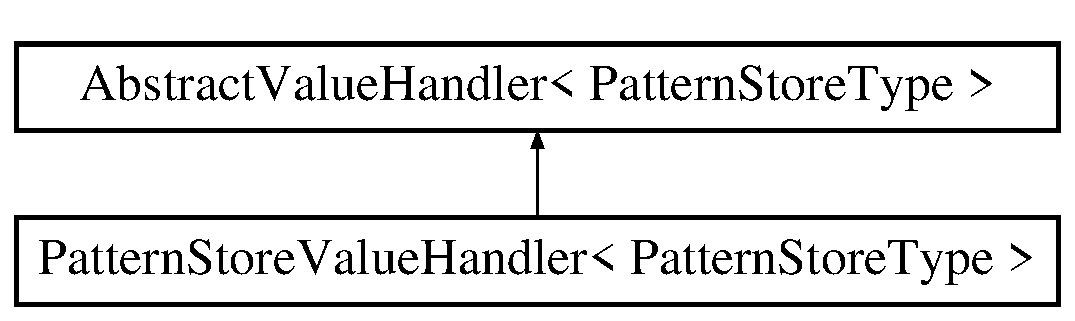
\includegraphics[height=2.000000cm]{classPatternStoreValueHandler}
\end{center}
\end{figure}
\subsection*{Public Member Functions}
\begin{DoxyCompactItemize}
\item 
virtual std\+::string \hyperlink{classPatternStoreValueHandler_a8f1745d36fe84bd8b96854a30b3bc5f7}{id} ()
\item 
void \hyperlink{classPatternStoreValueHandler_a1ee31fd587f60c2c10200581724fbee6}{read} (std\+::istream $\ast$in, Pattern\+Store\+Type \&value)
\item 
void \hyperlink{classPatternStoreValueHandler_a64d152c70a8ffd4f5ffdb09abb570b2d}{write} (std\+::ostream $\ast$out, Pattern\+Store\+Type \&value)
\item 
virtual std\+::string \hyperlink{classPatternStoreValueHandler_ac976813f02dcad60eb8cb700c6ba0753}{tostring} (Pattern\+Store\+Type \&value)
\item 
unsigned int \hyperlink{classPatternStoreValueHandler_af967671eda3e9ab05c0bf05ca9d0dfae}{count} (Pattern\+Store\+Type \&value) const 
\item 
void \hyperlink{classPatternStoreValueHandler_af05f8053a126fa4a0b100a2a70258977}{add} (Pattern\+Store\+Type $\ast$value, const \hyperlink{classIndexReference}{Index\+Reference} \&ref) const 
\end{DoxyCompactItemize}
\subsection*{Static Public Attributes}
\begin{DoxyCompactItemize}
\item 
static const bool \hyperlink{classPatternStoreValueHandler_ad61eccf1c00feb4a743e977f2378768f}{indexed} = false
\end{DoxyCompactItemize}


\subsection{Detailed Description}
\subsubsection*{template$<$class Pattern\+Store\+Type$>$class Pattern\+Store\+Value\+Handler$<$ Pattern\+Store\+Type $>$}

A complex value handler for values that are themselves pattern stores (allows building nested maps). 

\subsection{Member Function Documentation}
\hypertarget{classPatternStoreValueHandler_af05f8053a126fa4a0b100a2a70258977}{}\index{Pattern\+Store\+Value\+Handler@{Pattern\+Store\+Value\+Handler}!add@{add}}
\index{add@{add}!Pattern\+Store\+Value\+Handler@{Pattern\+Store\+Value\+Handler}}
\subsubsection[{add(\+Pattern\+Store\+Type $\ast$value, const Index\+Reference \&ref) const }]{\setlength{\rightskip}{0pt plus 5cm}template$<$class Pattern\+Store\+Type$>$ void {\bf Pattern\+Store\+Value\+Handler}$<$ Pattern\+Store\+Type $>$\+::add (
\begin{DoxyParamCaption}
\item[{Pattern\+Store\+Type $\ast$}]{value, }
\item[{const {\bf Index\+Reference} \&}]{ref}
\end{DoxyParamCaption}
) const\hspace{0.3cm}{\ttfamily [inline]}, {\ttfamily [virtual]}}\label{classPatternStoreValueHandler_af05f8053a126fa4a0b100a2a70258977}


Implements \hyperlink{classAbstractValueHandler_a72ecec2580cb5a9a3ba1495a98d08d98}{Abstract\+Value\+Handler$<$ Pattern\+Store\+Type $>$}.

\hypertarget{classPatternStoreValueHandler_af967671eda3e9ab05c0bf05ca9d0dfae}{}\index{Pattern\+Store\+Value\+Handler@{Pattern\+Store\+Value\+Handler}!count@{count}}
\index{count@{count}!Pattern\+Store\+Value\+Handler@{Pattern\+Store\+Value\+Handler}}
\subsubsection[{count(\+Pattern\+Store\+Type \&value) const }]{\setlength{\rightskip}{0pt plus 5cm}template$<$class Pattern\+Store\+Type$>$ unsigned int {\bf Pattern\+Store\+Value\+Handler}$<$ Pattern\+Store\+Type $>$\+::count (
\begin{DoxyParamCaption}
\item[{Pattern\+Store\+Type \&}]{value}
\end{DoxyParamCaption}
) const\hspace{0.3cm}{\ttfamily [inline]}, {\ttfamily [virtual]}}\label{classPatternStoreValueHandler_af967671eda3e9ab05c0bf05ca9d0dfae}


Implements \hyperlink{classAbstractValueHandler_a1d5941f6ff2afaee0c0bfc89ccb5188e}{Abstract\+Value\+Handler$<$ Pattern\+Store\+Type $>$}.

\hypertarget{classPatternStoreValueHandler_a8f1745d36fe84bd8b96854a30b3bc5f7}{}\index{Pattern\+Store\+Value\+Handler@{Pattern\+Store\+Value\+Handler}!id@{id}}
\index{id@{id}!Pattern\+Store\+Value\+Handler@{Pattern\+Store\+Value\+Handler}}
\subsubsection[{id()}]{\setlength{\rightskip}{0pt plus 5cm}template$<$class Pattern\+Store\+Type$>$ virtual std\+::string {\bf Pattern\+Store\+Value\+Handler}$<$ Pattern\+Store\+Type $>$\+::id (
\begin{DoxyParamCaption}
{}
\end{DoxyParamCaption}
)\hspace{0.3cm}{\ttfamily [inline]}, {\ttfamily [virtual]}}\label{classPatternStoreValueHandler_a8f1745d36fe84bd8b96854a30b3bc5f7}


Reimplemented from \hyperlink{classAbstractValueHandler_a6e2f7abe130cdec1062e51d56e4f9fac}{Abstract\+Value\+Handler$<$ Pattern\+Store\+Type $>$}.

\hypertarget{classPatternStoreValueHandler_a1ee31fd587f60c2c10200581724fbee6}{}\index{Pattern\+Store\+Value\+Handler@{Pattern\+Store\+Value\+Handler}!read@{read}}
\index{read@{read}!Pattern\+Store\+Value\+Handler@{Pattern\+Store\+Value\+Handler}}
\subsubsection[{read(std\+::istream $\ast$in, Pattern\+Store\+Type \&value)}]{\setlength{\rightskip}{0pt plus 5cm}template$<$class Pattern\+Store\+Type$>$ void {\bf Pattern\+Store\+Value\+Handler}$<$ Pattern\+Store\+Type $>$\+::read (
\begin{DoxyParamCaption}
\item[{std\+::istream $\ast$}]{in, }
\item[{Pattern\+Store\+Type \&}]{value}
\end{DoxyParamCaption}
)\hspace{0.3cm}{\ttfamily [inline]}, {\ttfamily [virtual]}}\label{classPatternStoreValueHandler_a1ee31fd587f60c2c10200581724fbee6}


Implements \hyperlink{classAbstractValueHandler_ac7921fae157361b054e467bf96785654}{Abstract\+Value\+Handler$<$ Pattern\+Store\+Type $>$}.

\hypertarget{classPatternStoreValueHandler_ac976813f02dcad60eb8cb700c6ba0753}{}\index{Pattern\+Store\+Value\+Handler@{Pattern\+Store\+Value\+Handler}!tostring@{tostring}}
\index{tostring@{tostring}!Pattern\+Store\+Value\+Handler@{Pattern\+Store\+Value\+Handler}}
\subsubsection[{tostring(\+Pattern\+Store\+Type \&value)}]{\setlength{\rightskip}{0pt plus 5cm}template$<$class Pattern\+Store\+Type$>$ virtual std\+::string {\bf Pattern\+Store\+Value\+Handler}$<$ Pattern\+Store\+Type $>$\+::tostring (
\begin{DoxyParamCaption}
\item[{Pattern\+Store\+Type \&}]{value}
\end{DoxyParamCaption}
)\hspace{0.3cm}{\ttfamily [inline]}, {\ttfamily [virtual]}}\label{classPatternStoreValueHandler_ac976813f02dcad60eb8cb700c6ba0753}


Implements \hyperlink{classAbstractValueHandler_a8e56e3bbccc464a47a666352249e6a1b}{Abstract\+Value\+Handler$<$ Pattern\+Store\+Type $>$}.

\hypertarget{classPatternStoreValueHandler_a64d152c70a8ffd4f5ffdb09abb570b2d}{}\index{Pattern\+Store\+Value\+Handler@{Pattern\+Store\+Value\+Handler}!write@{write}}
\index{write@{write}!Pattern\+Store\+Value\+Handler@{Pattern\+Store\+Value\+Handler}}
\subsubsection[{write(std\+::ostream $\ast$out, Pattern\+Store\+Type \&value)}]{\setlength{\rightskip}{0pt plus 5cm}template$<$class Pattern\+Store\+Type$>$ void {\bf Pattern\+Store\+Value\+Handler}$<$ Pattern\+Store\+Type $>$\+::write (
\begin{DoxyParamCaption}
\item[{std\+::ostream $\ast$}]{out, }
\item[{Pattern\+Store\+Type \&}]{value}
\end{DoxyParamCaption}
)\hspace{0.3cm}{\ttfamily [inline]}, {\ttfamily [virtual]}}\label{classPatternStoreValueHandler_a64d152c70a8ffd4f5ffdb09abb570b2d}


Implements \hyperlink{classAbstractValueHandler_aecd2820bc132f8065babbec5cd7458b8}{Abstract\+Value\+Handler$<$ Pattern\+Store\+Type $>$}.



\subsection{Member Data Documentation}
\hypertarget{classPatternStoreValueHandler_ad61eccf1c00feb4a743e977f2378768f}{}\index{Pattern\+Store\+Value\+Handler@{Pattern\+Store\+Value\+Handler}!indexed@{indexed}}
\index{indexed@{indexed}!Pattern\+Store\+Value\+Handler@{Pattern\+Store\+Value\+Handler}}
\subsubsection[{indexed}]{\setlength{\rightskip}{0pt plus 5cm}template$<$class Pattern\+Store\+Type$>$ const bool {\bf Pattern\+Store\+Value\+Handler}$<$ Pattern\+Store\+Type $>$\+::indexed = false\hspace{0.3cm}{\ttfamily [static]}}\label{classPatternStoreValueHandler_ad61eccf1c00feb4a743e977f2378768f}


The documentation for this class was generated from the following file\+:\begin{DoxyCompactItemize}
\item 
include/\hyperlink{patternstore_8h}{patternstore.\+h}\end{DoxyCompactItemize}

\hypertarget{classSpookyHash}{}\section{Spooky\+Hash Class Reference}
\label{classSpookyHash}\index{Spooky\+Hash@{Spooky\+Hash}}


{\ttfamily \#include $<$Spooky\+V2.\+h$>$}

\subsection*{Public Member Functions}
\begin{DoxyCompactItemize}
\item 
void \hyperlink{classSpookyHash_acba9d3327d8576d4126b15f301a17282}{Init} (\hyperlink{SpookyV2_8h_abc0f5bc07737e498f287334775dff2b6}{uint64} seed1, \hyperlink{SpookyV2_8h_abc0f5bc07737e498f287334775dff2b6}{uint64} seed2)
\item 
void \hyperlink{classSpookyHash_a1a95761b21aa9d827ad9b62f56a30877}{Update} (const void $\ast$message, size\+\_\+t length)
\item 
void \hyperlink{classSpookyHash_ae37b93d6c4386e1879cec667ab6c103e}{Final} (\hyperlink{SpookyV2_8h_abc0f5bc07737e498f287334775dff2b6}{uint64} $\ast$hash1, \hyperlink{SpookyV2_8h_abc0f5bc07737e498f287334775dff2b6}{uint64} $\ast$hash2)
\end{DoxyCompactItemize}
\subsection*{Static Public Member Functions}
\begin{DoxyCompactItemize}
\item 
static void \hyperlink{classSpookyHash_a9d8973d46becbc8036c458fae3efc3a5}{Hash128} (const void $\ast$message, size\+\_\+t length, \hyperlink{SpookyV2_8h_abc0f5bc07737e498f287334775dff2b6}{uint64} $\ast$hash1, \hyperlink{SpookyV2_8h_abc0f5bc07737e498f287334775dff2b6}{uint64} $\ast$hash2)
\item 
static \hyperlink{SpookyV2_8h_abc0f5bc07737e498f287334775dff2b6}{uint64} \hyperlink{classSpookyHash_a4781c0814a39002c57900a108f3005f0}{Hash64} (const void $\ast$message, size\+\_\+t length, \hyperlink{SpookyV2_8h_abc0f5bc07737e498f287334775dff2b6}{uint64} seed=0)
\item 
static \hyperlink{SpookyV2_8h_acbd4acd0d29e2d6c43104827f77d9cd2}{uint32} \hyperlink{classSpookyHash_a73d8524c291fccbc319517341abb2f77}{Hash32} (const void $\ast$message, size\+\_\+t length, \hyperlink{SpookyV2_8h_acbd4acd0d29e2d6c43104827f77d9cd2}{uint32} seed=0)
\item 
static \hyperlink{SpookyV2_8h_a2eb6f9e0395b47b8d5e3eeae4fe0c116}{I\+N\+L\+I\+N\+E} \hyperlink{SpookyV2_8h_abc0f5bc07737e498f287334775dff2b6}{uint64} \hyperlink{classSpookyHash_a2b3b07af28a0b4f0f920fdb3a31a0c87}{Rot64} (\hyperlink{SpookyV2_8h_abc0f5bc07737e498f287334775dff2b6}{uint64} x, int k)
\item 
static \hyperlink{SpookyV2_8h_a2eb6f9e0395b47b8d5e3eeae4fe0c116}{I\+N\+L\+I\+N\+E} void \hyperlink{classSpookyHash_a749e6012af3d67884a323e227105e032}{Mix} (const \hyperlink{SpookyV2_8h_abc0f5bc07737e498f287334775dff2b6}{uint64} $\ast$data, \hyperlink{SpookyV2_8h_abc0f5bc07737e498f287334775dff2b6}{uint64} \&s0, \hyperlink{SpookyV2_8h_abc0f5bc07737e498f287334775dff2b6}{uint64} \&s1, \hyperlink{SpookyV2_8h_abc0f5bc07737e498f287334775dff2b6}{uint64} \&s2, \hyperlink{SpookyV2_8h_abc0f5bc07737e498f287334775dff2b6}{uint64} \&s3, \hyperlink{SpookyV2_8h_abc0f5bc07737e498f287334775dff2b6}{uint64} \&s4, \hyperlink{SpookyV2_8h_abc0f5bc07737e498f287334775dff2b6}{uint64} \&s5, \hyperlink{SpookyV2_8h_abc0f5bc07737e498f287334775dff2b6}{uint64} \&s6, \hyperlink{SpookyV2_8h_abc0f5bc07737e498f287334775dff2b6}{uint64} \&s7, \hyperlink{SpookyV2_8h_abc0f5bc07737e498f287334775dff2b6}{uint64} \&s8, \hyperlink{SpookyV2_8h_abc0f5bc07737e498f287334775dff2b6}{uint64} \&s9, \hyperlink{SpookyV2_8h_abc0f5bc07737e498f287334775dff2b6}{uint64} \&s10, \hyperlink{SpookyV2_8h_abc0f5bc07737e498f287334775dff2b6}{uint64} \&s11)
\item 
static \hyperlink{SpookyV2_8h_a2eb6f9e0395b47b8d5e3eeae4fe0c116}{I\+N\+L\+I\+N\+E} void \hyperlink{classSpookyHash_a9799c4b36e1c73e895e4e7293eb94521}{End\+Partial} (\hyperlink{SpookyV2_8h_abc0f5bc07737e498f287334775dff2b6}{uint64} \&h0, \hyperlink{SpookyV2_8h_abc0f5bc07737e498f287334775dff2b6}{uint64} \&h1, \hyperlink{SpookyV2_8h_abc0f5bc07737e498f287334775dff2b6}{uint64} \&h2, \hyperlink{SpookyV2_8h_abc0f5bc07737e498f287334775dff2b6}{uint64} \&h3, \hyperlink{SpookyV2_8h_abc0f5bc07737e498f287334775dff2b6}{uint64} \&h4, \hyperlink{SpookyV2_8h_abc0f5bc07737e498f287334775dff2b6}{uint64} \&h5, \hyperlink{SpookyV2_8h_abc0f5bc07737e498f287334775dff2b6}{uint64} \&h6, \hyperlink{SpookyV2_8h_abc0f5bc07737e498f287334775dff2b6}{uint64} \&h7, \hyperlink{SpookyV2_8h_abc0f5bc07737e498f287334775dff2b6}{uint64} \&h8, \hyperlink{SpookyV2_8h_abc0f5bc07737e498f287334775dff2b6}{uint64} \&h9, \hyperlink{SpookyV2_8h_abc0f5bc07737e498f287334775dff2b6}{uint64} \&h10, \hyperlink{SpookyV2_8h_abc0f5bc07737e498f287334775dff2b6}{uint64} \&h11)
\item 
static \hyperlink{SpookyV2_8h_a2eb6f9e0395b47b8d5e3eeae4fe0c116}{I\+N\+L\+I\+N\+E} void \hyperlink{classSpookyHash_a21b8777af68b866653ac4de06df9416f}{End} (const \hyperlink{SpookyV2_8h_abc0f5bc07737e498f287334775dff2b6}{uint64} $\ast$data, \hyperlink{SpookyV2_8h_abc0f5bc07737e498f287334775dff2b6}{uint64} \&h0, \hyperlink{SpookyV2_8h_abc0f5bc07737e498f287334775dff2b6}{uint64} \&h1, \hyperlink{SpookyV2_8h_abc0f5bc07737e498f287334775dff2b6}{uint64} \&h2, \hyperlink{SpookyV2_8h_abc0f5bc07737e498f287334775dff2b6}{uint64} \&h3, \hyperlink{SpookyV2_8h_abc0f5bc07737e498f287334775dff2b6}{uint64} \&h4, \hyperlink{SpookyV2_8h_abc0f5bc07737e498f287334775dff2b6}{uint64} \&h5, \hyperlink{SpookyV2_8h_abc0f5bc07737e498f287334775dff2b6}{uint64} \&h6, \hyperlink{SpookyV2_8h_abc0f5bc07737e498f287334775dff2b6}{uint64} \&h7, \hyperlink{SpookyV2_8h_abc0f5bc07737e498f287334775dff2b6}{uint64} \&h8, \hyperlink{SpookyV2_8h_abc0f5bc07737e498f287334775dff2b6}{uint64} \&h9, \hyperlink{SpookyV2_8h_abc0f5bc07737e498f287334775dff2b6}{uint64} \&h10, \hyperlink{SpookyV2_8h_abc0f5bc07737e498f287334775dff2b6}{uint64} \&h11)
\item 
static \hyperlink{SpookyV2_8h_a2eb6f9e0395b47b8d5e3eeae4fe0c116}{I\+N\+L\+I\+N\+E} void \hyperlink{classSpookyHash_a2a18b61b405f43f283ba9a20016b5b9f}{Short\+Mix} (\hyperlink{SpookyV2_8h_abc0f5bc07737e498f287334775dff2b6}{uint64} \&h0, \hyperlink{SpookyV2_8h_abc0f5bc07737e498f287334775dff2b6}{uint64} \&h1, \hyperlink{SpookyV2_8h_abc0f5bc07737e498f287334775dff2b6}{uint64} \&h2, \hyperlink{SpookyV2_8h_abc0f5bc07737e498f287334775dff2b6}{uint64} \&h3)
\item 
static \hyperlink{SpookyV2_8h_a2eb6f9e0395b47b8d5e3eeae4fe0c116}{I\+N\+L\+I\+N\+E} void \hyperlink{classSpookyHash_a5b01b1a2b3270e9c11244a6702b0db59}{Short\+End} (\hyperlink{SpookyV2_8h_abc0f5bc07737e498f287334775dff2b6}{uint64} \&h0, \hyperlink{SpookyV2_8h_abc0f5bc07737e498f287334775dff2b6}{uint64} \&h1, \hyperlink{SpookyV2_8h_abc0f5bc07737e498f287334775dff2b6}{uint64} \&h2, \hyperlink{SpookyV2_8h_abc0f5bc07737e498f287334775dff2b6}{uint64} \&h3)
\end{DoxyCompactItemize}


\subsection{Member Function Documentation}
\hypertarget{classSpookyHash_a21b8777af68b866653ac4de06df9416f}{}\index{Spooky\+Hash@{Spooky\+Hash}!End@{End}}
\index{End@{End}!Spooky\+Hash@{Spooky\+Hash}}
\subsubsection[{End(const uint64 $\ast$data, uint64 \&h0, uint64 \&h1, uint64 \&h2, uint64 \&h3, uint64 \&h4, uint64 \&h5, uint64 \&h6, uint64 \&h7, uint64 \&h8, uint64 \&h9, uint64 \&h10, uint64 \&h11)}]{\setlength{\rightskip}{0pt plus 5cm}static {\bf I\+N\+L\+I\+N\+E} void Spooky\+Hash\+::\+End (
\begin{DoxyParamCaption}
\item[{const {\bf uint64} $\ast$}]{data, }
\item[{{\bf uint64} \&}]{h0, }
\item[{{\bf uint64} \&}]{h1, }
\item[{{\bf uint64} \&}]{h2, }
\item[{{\bf uint64} \&}]{h3, }
\item[{{\bf uint64} \&}]{h4, }
\item[{{\bf uint64} \&}]{h5, }
\item[{{\bf uint64} \&}]{h6, }
\item[{{\bf uint64} \&}]{h7, }
\item[{{\bf uint64} \&}]{h8, }
\item[{{\bf uint64} \&}]{h9, }
\item[{{\bf uint64} \&}]{h10, }
\item[{{\bf uint64} \&}]{h11}
\end{DoxyParamCaption}
)\hspace{0.3cm}{\ttfamily [inline]}, {\ttfamily [static]}}\label{classSpookyHash_a21b8777af68b866653ac4de06df9416f}
\hypertarget{classSpookyHash_a9799c4b36e1c73e895e4e7293eb94521}{}\index{Spooky\+Hash@{Spooky\+Hash}!End\+Partial@{End\+Partial}}
\index{End\+Partial@{End\+Partial}!Spooky\+Hash@{Spooky\+Hash}}
\subsubsection[{End\+Partial(uint64 \&h0, uint64 \&h1, uint64 \&h2, uint64 \&h3, uint64 \&h4, uint64 \&h5, uint64 \&h6, uint64 \&h7, uint64 \&h8, uint64 \&h9, uint64 \&h10, uint64 \&h11)}]{\setlength{\rightskip}{0pt plus 5cm}static {\bf I\+N\+L\+I\+N\+E} void Spooky\+Hash\+::\+End\+Partial (
\begin{DoxyParamCaption}
\item[{{\bf uint64} \&}]{h0, }
\item[{{\bf uint64} \&}]{h1, }
\item[{{\bf uint64} \&}]{h2, }
\item[{{\bf uint64} \&}]{h3, }
\item[{{\bf uint64} \&}]{h4, }
\item[{{\bf uint64} \&}]{h5, }
\item[{{\bf uint64} \&}]{h6, }
\item[{{\bf uint64} \&}]{h7, }
\item[{{\bf uint64} \&}]{h8, }
\item[{{\bf uint64} \&}]{h9, }
\item[{{\bf uint64} \&}]{h10, }
\item[{{\bf uint64} \&}]{h11}
\end{DoxyParamCaption}
)\hspace{0.3cm}{\ttfamily [inline]}, {\ttfamily [static]}}\label{classSpookyHash_a9799c4b36e1c73e895e4e7293eb94521}
\hypertarget{classSpookyHash_ae37b93d6c4386e1879cec667ab6c103e}{}\index{Spooky\+Hash@{Spooky\+Hash}!Final@{Final}}
\index{Final@{Final}!Spooky\+Hash@{Spooky\+Hash}}
\subsubsection[{Final(uint64 $\ast$hash1, uint64 $\ast$hash2)}]{\setlength{\rightskip}{0pt plus 5cm}void Spooky\+Hash\+::\+Final (
\begin{DoxyParamCaption}
\item[{{\bf uint64} $\ast$}]{hash1, }
\item[{{\bf uint64} $\ast$}]{hash2}
\end{DoxyParamCaption}
)}\label{classSpookyHash_ae37b93d6c4386e1879cec667ab6c103e}
\hypertarget{classSpookyHash_a9d8973d46becbc8036c458fae3efc3a5}{}\index{Spooky\+Hash@{Spooky\+Hash}!Hash128@{Hash128}}
\index{Hash128@{Hash128}!Spooky\+Hash@{Spooky\+Hash}}
\subsubsection[{Hash128(const void $\ast$message, size\+\_\+t length, uint64 $\ast$hash1, uint64 $\ast$hash2)}]{\setlength{\rightskip}{0pt plus 5cm}void Spooky\+Hash\+::\+Hash128 (
\begin{DoxyParamCaption}
\item[{const void $\ast$}]{message, }
\item[{size\+\_\+t}]{length, }
\item[{{\bf uint64} $\ast$}]{hash1, }
\item[{{\bf uint64} $\ast$}]{hash2}
\end{DoxyParamCaption}
)\hspace{0.3cm}{\ttfamily [static]}}\label{classSpookyHash_a9d8973d46becbc8036c458fae3efc3a5}
\hypertarget{classSpookyHash_a73d8524c291fccbc319517341abb2f77}{}\index{Spooky\+Hash@{Spooky\+Hash}!Hash32@{Hash32}}
\index{Hash32@{Hash32}!Spooky\+Hash@{Spooky\+Hash}}
\subsubsection[{Hash32(const void $\ast$message, size\+\_\+t length, uint32 seed=0)}]{\setlength{\rightskip}{0pt plus 5cm}static {\bf uint32} Spooky\+Hash\+::\+Hash32 (
\begin{DoxyParamCaption}
\item[{const void $\ast$}]{message, }
\item[{size\+\_\+t}]{length, }
\item[{{\bf uint32}}]{seed = {\ttfamily 0}}
\end{DoxyParamCaption}
)\hspace{0.3cm}{\ttfamily [inline]}, {\ttfamily [static]}}\label{classSpookyHash_a73d8524c291fccbc319517341abb2f77}
\hypertarget{classSpookyHash_a4781c0814a39002c57900a108f3005f0}{}\index{Spooky\+Hash@{Spooky\+Hash}!Hash64@{Hash64}}
\index{Hash64@{Hash64}!Spooky\+Hash@{Spooky\+Hash}}
\subsubsection[{Hash64(const void $\ast$message, size\+\_\+t length, uint64 seed=0)}]{\setlength{\rightskip}{0pt plus 5cm}static {\bf uint64} Spooky\+Hash\+::\+Hash64 (
\begin{DoxyParamCaption}
\item[{const void $\ast$}]{message, }
\item[{size\+\_\+t}]{length, }
\item[{{\bf uint64}}]{seed = {\ttfamily 0}}
\end{DoxyParamCaption}
)\hspace{0.3cm}{\ttfamily [inline]}, {\ttfamily [static]}}\label{classSpookyHash_a4781c0814a39002c57900a108f3005f0}
\hypertarget{classSpookyHash_acba9d3327d8576d4126b15f301a17282}{}\index{Spooky\+Hash@{Spooky\+Hash}!Init@{Init}}
\index{Init@{Init}!Spooky\+Hash@{Spooky\+Hash}}
\subsubsection[{Init(uint64 seed1, uint64 seed2)}]{\setlength{\rightskip}{0pt plus 5cm}void Spooky\+Hash\+::\+Init (
\begin{DoxyParamCaption}
\item[{{\bf uint64}}]{seed1, }
\item[{{\bf uint64}}]{seed2}
\end{DoxyParamCaption}
)}\label{classSpookyHash_acba9d3327d8576d4126b15f301a17282}
\hypertarget{classSpookyHash_a749e6012af3d67884a323e227105e032}{}\index{Spooky\+Hash@{Spooky\+Hash}!Mix@{Mix}}
\index{Mix@{Mix}!Spooky\+Hash@{Spooky\+Hash}}
\subsubsection[{Mix(const uint64 $\ast$data, uint64 \&s0, uint64 \&s1, uint64 \&s2, uint64 \&s3, uint64 \&s4, uint64 \&s5, uint64 \&s6, uint64 \&s7, uint64 \&s8, uint64 \&s9, uint64 \&s10, uint64 \&s11)}]{\setlength{\rightskip}{0pt plus 5cm}static {\bf I\+N\+L\+I\+N\+E} void Spooky\+Hash\+::\+Mix (
\begin{DoxyParamCaption}
\item[{const {\bf uint64} $\ast$}]{data, }
\item[{{\bf uint64} \&}]{s0, }
\item[{{\bf uint64} \&}]{s1, }
\item[{{\bf uint64} \&}]{s2, }
\item[{{\bf uint64} \&}]{s3, }
\item[{{\bf uint64} \&}]{s4, }
\item[{{\bf uint64} \&}]{s5, }
\item[{{\bf uint64} \&}]{s6, }
\item[{{\bf uint64} \&}]{s7, }
\item[{{\bf uint64} \&}]{s8, }
\item[{{\bf uint64} \&}]{s9, }
\item[{{\bf uint64} \&}]{s10, }
\item[{{\bf uint64} \&}]{s11}
\end{DoxyParamCaption}
)\hspace{0.3cm}{\ttfamily [inline]}, {\ttfamily [static]}}\label{classSpookyHash_a749e6012af3d67884a323e227105e032}
\hypertarget{classSpookyHash_a2b3b07af28a0b4f0f920fdb3a31a0c87}{}\index{Spooky\+Hash@{Spooky\+Hash}!Rot64@{Rot64}}
\index{Rot64@{Rot64}!Spooky\+Hash@{Spooky\+Hash}}
\subsubsection[{Rot64(uint64 x, int k)}]{\setlength{\rightskip}{0pt plus 5cm}static {\bf I\+N\+L\+I\+N\+E} {\bf uint64} Spooky\+Hash\+::\+Rot64 (
\begin{DoxyParamCaption}
\item[{{\bf uint64}}]{x, }
\item[{int}]{k}
\end{DoxyParamCaption}
)\hspace{0.3cm}{\ttfamily [inline]}, {\ttfamily [static]}}\label{classSpookyHash_a2b3b07af28a0b4f0f920fdb3a31a0c87}
\hypertarget{classSpookyHash_a5b01b1a2b3270e9c11244a6702b0db59}{}\index{Spooky\+Hash@{Spooky\+Hash}!Short\+End@{Short\+End}}
\index{Short\+End@{Short\+End}!Spooky\+Hash@{Spooky\+Hash}}
\subsubsection[{Short\+End(uint64 \&h0, uint64 \&h1, uint64 \&h2, uint64 \&h3)}]{\setlength{\rightskip}{0pt plus 5cm}static {\bf I\+N\+L\+I\+N\+E} void Spooky\+Hash\+::\+Short\+End (
\begin{DoxyParamCaption}
\item[{{\bf uint64} \&}]{h0, }
\item[{{\bf uint64} \&}]{h1, }
\item[{{\bf uint64} \&}]{h2, }
\item[{{\bf uint64} \&}]{h3}
\end{DoxyParamCaption}
)\hspace{0.3cm}{\ttfamily [inline]}, {\ttfamily [static]}}\label{classSpookyHash_a5b01b1a2b3270e9c11244a6702b0db59}
\hypertarget{classSpookyHash_a2a18b61b405f43f283ba9a20016b5b9f}{}\index{Spooky\+Hash@{Spooky\+Hash}!Short\+Mix@{Short\+Mix}}
\index{Short\+Mix@{Short\+Mix}!Spooky\+Hash@{Spooky\+Hash}}
\subsubsection[{Short\+Mix(uint64 \&h0, uint64 \&h1, uint64 \&h2, uint64 \&h3)}]{\setlength{\rightskip}{0pt plus 5cm}static {\bf I\+N\+L\+I\+N\+E} void Spooky\+Hash\+::\+Short\+Mix (
\begin{DoxyParamCaption}
\item[{{\bf uint64} \&}]{h0, }
\item[{{\bf uint64} \&}]{h1, }
\item[{{\bf uint64} \&}]{h2, }
\item[{{\bf uint64} \&}]{h3}
\end{DoxyParamCaption}
)\hspace{0.3cm}{\ttfamily [inline]}, {\ttfamily [static]}}\label{classSpookyHash_a2a18b61b405f43f283ba9a20016b5b9f}
\hypertarget{classSpookyHash_a1a95761b21aa9d827ad9b62f56a30877}{}\index{Spooky\+Hash@{Spooky\+Hash}!Update@{Update}}
\index{Update@{Update}!Spooky\+Hash@{Spooky\+Hash}}
\subsubsection[{Update(const void $\ast$message, size\+\_\+t length)}]{\setlength{\rightskip}{0pt plus 5cm}void Spooky\+Hash\+::\+Update (
\begin{DoxyParamCaption}
\item[{const void $\ast$}]{message, }
\item[{size\+\_\+t}]{length}
\end{DoxyParamCaption}
)}\label{classSpookyHash_a1a95761b21aa9d827ad9b62f56a30877}


The documentation for this class was generated from the following files\+:\begin{DoxyCompactItemize}
\item 
include/\hyperlink{SpookyV2_8h}{Spooky\+V2.\+h}\item 
src/\hyperlink{SpookyV2_8cpp}{Spooky\+V2.\+cpp}\end{DoxyCompactItemize}

\chapter{File Documentation}
\hypertarget{algorithms_8h}{}\section{include/algorithms.h File Reference}
\label{algorithms_8h}\index{include/algorithms.\+h@{include/algorithms.\+h}}
{\ttfamily \#include $<$unordered\+\_\+map$>$}\\*
{\ttfamily \#include $<$vector$>$}\\*
{\ttfamily \#include $<$utility$>$}\\*
{\ttfamily \#include $<$cstdint$>$}\\*
{\ttfamily \#include \char`\"{}common.\+h\char`\"{}}\\*
\subsection*{Functions}
\begin{DoxyCompactItemize}
\item 
uint32\+\_\+t \hyperlink{algorithms_8h_a83c677ca972ac87e4bce9008eebcb07e}{vector2mask} (const std\+::vector$<$ std\+::pair$<$ int, int $>$$>$ \&skips)
\item 
std\+::vector$<$ std\+::pair$<$ int, int $>$ $>$ \hyperlink{algorithms_8h_a9ca13d16372b52cb0b2bf058f58fce63}{mask2vector} (const uint32\+\_\+t mask, const int n)
\item 
std\+::vector$<$ std\+::pair$<$ int, int $>$ $>$ \hyperlink{algorithms_8h_aebb50b68f3aea347fb004b525fb9a84a}{get\+\_\+consecutive\+\_\+gaps} (const int n, const int leftmargin=1, const int rightmargin=1)
\item 
uint32\+\_\+t \hyperlink{algorithms_8h_ac8b732f37fb89fb5edacfbc9d3b95356}{reversemask} (uint32\+\_\+t mask, const unsigned int n)
\item 
int \hyperlink{algorithms_8h_aed39efadda0e0c9a9caeec74ad25be79}{maskheadskip} (uint32\+\_\+t mask, const unsigned int n)
\item 
int \hyperlink{algorithms_8h_a1c0cdba6c75aa2680062858530c0eaf8}{masktailskip} (uint32\+\_\+t mask, const unsigned int n)
\item 
std\+::vector$<$ uint32\+\_\+t $>$ \hyperlink{algorithms_8h_a50886ebc1499d851fd7161227f1ae2df}{compute\+\_\+skip\+\_\+configurations} (const int n, const int maxskips)
\end{DoxyCompactItemize}


\subsection{Function Documentation}
\hypertarget{algorithms_8h_a50886ebc1499d851fd7161227f1ae2df}{}\index{algorithms.\+h@{algorithms.\+h}!compute\+\_\+skip\+\_\+configurations@{compute\+\_\+skip\+\_\+configurations}}
\index{compute\+\_\+skip\+\_\+configurations@{compute\+\_\+skip\+\_\+configurations}!algorithms.\+h@{algorithms.\+h}}
\subsubsection[{compute\+\_\+skip\+\_\+configurations(const int n, const int maxskips)}]{\setlength{\rightskip}{0pt plus 5cm}std\+::vector$<$uint32\+\_\+t$>$ compute\+\_\+skip\+\_\+configurations (
\begin{DoxyParamCaption}
\item[{const int}]{n, }
\item[{const int}]{maxskips}
\end{DoxyParamCaption}
)}\label{algorithms_8h_a50886ebc1499d851fd7161227f1ae2df}
\hypertarget{algorithms_8h_aebb50b68f3aea347fb004b525fb9a84a}{}\index{algorithms.\+h@{algorithms.\+h}!get\+\_\+consecutive\+\_\+gaps@{get\+\_\+consecutive\+\_\+gaps}}
\index{get\+\_\+consecutive\+\_\+gaps@{get\+\_\+consecutive\+\_\+gaps}!algorithms.\+h@{algorithms.\+h}}
\subsubsection[{get\+\_\+consecutive\+\_\+gaps(const int n, const int leftmargin=1, const int rightmargin=1)}]{\setlength{\rightskip}{0pt plus 5cm}std\+::vector$<$ std\+::pair$<$int,int$>$ $>$ get\+\_\+consecutive\+\_\+gaps (
\begin{DoxyParamCaption}
\item[{const int}]{n, }
\item[{const int}]{leftmargin = {\ttfamily 1}, }
\item[{const int}]{rightmargin = {\ttfamily 1}}
\end{DoxyParamCaption}
)}\label{algorithms_8h_aebb50b68f3aea347fb004b525fb9a84a}
\hypertarget{algorithms_8h_a9ca13d16372b52cb0b2bf058f58fce63}{}\index{algorithms.\+h@{algorithms.\+h}!mask2vector@{mask2vector}}
\index{mask2vector@{mask2vector}!algorithms.\+h@{algorithms.\+h}}
\subsubsection[{mask2vector(const uint32\+\_\+t mask, const int n)}]{\setlength{\rightskip}{0pt plus 5cm}std\+::vector$<$std\+::pair$<$int,int$>$ $>$ mask2vector (
\begin{DoxyParamCaption}
\item[{const uint32\+\_\+t}]{mask, }
\item[{const int}]{n}
\end{DoxyParamCaption}
)}\label{algorithms_8h_a9ca13d16372b52cb0b2bf058f58fce63}
\hypertarget{algorithms_8h_aed39efadda0e0c9a9caeec74ad25be79}{}\index{algorithms.\+h@{algorithms.\+h}!maskheadskip@{maskheadskip}}
\index{maskheadskip@{maskheadskip}!algorithms.\+h@{algorithms.\+h}}
\subsubsection[{maskheadskip(uint32\+\_\+t mask, const unsigned int n)}]{\setlength{\rightskip}{0pt plus 5cm}int maskheadskip (
\begin{DoxyParamCaption}
\item[{uint32\+\_\+t}]{mask, }
\item[{const unsigned int}]{n}
\end{DoxyParamCaption}
)}\label{algorithms_8h_aed39efadda0e0c9a9caeec74ad25be79}
\hypertarget{algorithms_8h_a1c0cdba6c75aa2680062858530c0eaf8}{}\index{algorithms.\+h@{algorithms.\+h}!masktailskip@{masktailskip}}
\index{masktailskip@{masktailskip}!algorithms.\+h@{algorithms.\+h}}
\subsubsection[{masktailskip(uint32\+\_\+t mask, const unsigned int n)}]{\setlength{\rightskip}{0pt plus 5cm}int masktailskip (
\begin{DoxyParamCaption}
\item[{uint32\+\_\+t}]{mask, }
\item[{const unsigned int}]{n}
\end{DoxyParamCaption}
)}\label{algorithms_8h_a1c0cdba6c75aa2680062858530c0eaf8}
\hypertarget{algorithms_8h_ac8b732f37fb89fb5edacfbc9d3b95356}{}\index{algorithms.\+h@{algorithms.\+h}!reversemask@{reversemask}}
\index{reversemask@{reversemask}!algorithms.\+h@{algorithms.\+h}}
\subsubsection[{reversemask(uint32\+\_\+t mask, const unsigned int n)}]{\setlength{\rightskip}{0pt plus 5cm}uint32\+\_\+t reversemask (
\begin{DoxyParamCaption}
\item[{uint32\+\_\+t}]{mask, }
\item[{const unsigned int}]{n}
\end{DoxyParamCaption}
)}\label{algorithms_8h_ac8b732f37fb89fb5edacfbc9d3b95356}
\hypertarget{algorithms_8h_a83c677ca972ac87e4bce9008eebcb07e}{}\index{algorithms.\+h@{algorithms.\+h}!vector2mask@{vector2mask}}
\index{vector2mask@{vector2mask}!algorithms.\+h@{algorithms.\+h}}
\subsubsection[{vector2mask(const std\+::vector$<$ std\+::pair$<$ int, int $>$$>$ \&skips)}]{\setlength{\rightskip}{0pt plus 5cm}uint32\+\_\+t vector2mask (
\begin{DoxyParamCaption}
\item[{const std\+::vector$<$ std\+::pair$<$ int, int $>$$>$ \&}]{skips}
\end{DoxyParamCaption}
)}\label{algorithms_8h_a83c677ca972ac87e4bce9008eebcb07e}

\hypertarget{alignmodel_8h}{}\section{include/alignmodel.h File Reference}
\label{alignmodel_8h}\index{include/alignmodel.\+h@{include/alignmodel.\+h}}
{\ttfamily \#include \char`\"{}patternmodel.\+h\char`\"{}}\\*
\subsection*{Classes}
\begin{DoxyCompactItemize}
\item 
class \hyperlink{classPatternAlignmentModel}{Pattern\+Alignment\+Model$<$ Feature\+Type $>$}
\end{DoxyCompactItemize}

\hypertarget{classdecoder_8h}{}\section{include/classdecoder.h File Reference}
\label{classdecoder_8h}\index{include/classdecoder.\+h@{include/classdecoder.\+h}}


Class for decoding binary class-\/encoded data back to plain-\/text.  


{\ttfamily \#include $<$unordered\+\_\+map$>$}\\*
{\ttfamily \#include $<$string$>$}\\*
{\ttfamily \#include $<$vector$>$}\\*
{\ttfamily \#include $<$fstream$>$}\\*
\subsection*{Classes}
\begin{DoxyCompactItemize}
\item 
class \hyperlink{classClassDecoder}{Class\+Decoder}
\begin{DoxyCompactList}\small\item\em Class for decoding binary class-\/encoded data back to plain-\/text. The \hyperlink{classClassDecoder}{Class\+Decoder} maintains a mapping of classes (integers) to words. It allows decoding of a corpus that was losslessly compressed by substituting words for classes. The classes are distributed based on word frequency, with frequent words receiving a lower class number that can be represented in fewer bytes, and rare words receiving a higher class number. \end{DoxyCompactList}\end{DoxyCompactItemize}
\subsection*{Functions}
\begin{DoxyCompactItemize}
\item 
unsigned int \hyperlink{classdecoder_8h_aea9cc09167edc417a0176b44a4546aa9}{bytestoint} (const unsigned char $\ast$a, const int l)
\item 
int \hyperlink{classdecoder_8h_ad84aa03fdcbb1681ea715967a289e034}{readline} (std\+::istream $\ast$I\+N, unsigned char $\ast$buffer, const int)
\item 
const int \hyperlink{classdecoder_8h_a1c8dd71d61ed906899f173ce9942229d}{countwords} (const unsigned char $\ast$data, const int l)
\item 
std\+::pair$<$ int, int $>$ \hyperlink{classdecoder_8h_a50d64120d63b9df5dd49c00ac65c1d3b}{getwords} (const unsigned char $\ast$data, const int \hyperlink{pattern_8cpp_aa35f7c02f0b33f90cf30fca8eda3c712}{datasize}, const int n, const int begin=0)
\end{DoxyCompactItemize}


\subsection{Detailed Description}
Class for decoding binary class-\/encoded data back to plain-\/text. 

\begin{DoxyAuthor}{Author}
Maarten van Gompel (proycon) \href{mailto:proycon@anaproy.nl}{\tt proycon@anaproy.\+nl}
\end{DoxyAuthor}
\hypertarget{SpookyV2_8h_LICENSE}{}\subsection{L\+I\+C\+E\+N\+S\+E}\label{SpookyV2_8h_LICENSE}
Licensed under G\+P\+Lv3\hypertarget{SpookyV2_8h_DESCRIPTION}{}\subsection{D\+E\+S\+C\+R\+I\+P\+T\+I\+O\+N}\label{SpookyV2_8h_DESCRIPTION}
Class for decoding binary class-\/encoded data back to plain-\/text 

\subsection{Function Documentation}
\hypertarget{classdecoder_8h_aea9cc09167edc417a0176b44a4546aa9}{}\index{classdecoder.\+h@{classdecoder.\+h}!bytestoint@{bytestoint}}
\index{bytestoint@{bytestoint}!classdecoder.\+h@{classdecoder.\+h}}
\subsubsection[{bytestoint(const unsigned char $\ast$a, const int l)}]{\setlength{\rightskip}{0pt plus 5cm}unsigned int bytestoint (
\begin{DoxyParamCaption}
\item[{const unsigned char $\ast$}]{a, }
\item[{const int}]{l}
\end{DoxyParamCaption}
)}\label{classdecoder_8h_aea9cc09167edc417a0176b44a4546aa9}
\hypertarget{classdecoder_8h_a1c8dd71d61ed906899f173ce9942229d}{}\index{classdecoder.\+h@{classdecoder.\+h}!countwords@{countwords}}
\index{countwords@{countwords}!classdecoder.\+h@{classdecoder.\+h}}
\subsubsection[{countwords(const unsigned char $\ast$data, const int l)}]{\setlength{\rightskip}{0pt plus 5cm}const int countwords (
\begin{DoxyParamCaption}
\item[{const unsigned char $\ast$}]{data, }
\item[{const int}]{l}
\end{DoxyParamCaption}
)}\label{classdecoder_8h_a1c8dd71d61ed906899f173ce9942229d}
\hypertarget{classdecoder_8h_a50d64120d63b9df5dd49c00ac65c1d3b}{}\index{classdecoder.\+h@{classdecoder.\+h}!getwords@{getwords}}
\index{getwords@{getwords}!classdecoder.\+h@{classdecoder.\+h}}
\subsubsection[{getwords(const unsigned char $\ast$data, const int datasize, const int n, const int begin=0)}]{\setlength{\rightskip}{0pt plus 5cm}std\+::pair$<$int,int$>$ getwords (
\begin{DoxyParamCaption}
\item[{const unsigned char $\ast$}]{data, }
\item[{const int}]{datasize, }
\item[{const int}]{n, }
\item[{const int}]{begin = {\ttfamily 0}}
\end{DoxyParamCaption}
)}\label{classdecoder_8h_a50d64120d63b9df5dd49c00ac65c1d3b}
\hypertarget{classdecoder_8h_ad84aa03fdcbb1681ea715967a289e034}{}\index{classdecoder.\+h@{classdecoder.\+h}!readline@{readline}}
\index{readline@{readline}!classdecoder.\+h@{classdecoder.\+h}}
\subsubsection[{readline(std\+::istream $\ast$\+I\+N, unsigned char $\ast$buffer, const int)}]{\setlength{\rightskip}{0pt plus 5cm}int readline (
\begin{DoxyParamCaption}
\item[{std\+::istream $\ast$}]{I\+N, }
\item[{unsigned char $\ast$}]{buffer, }
\item[{const int}]{}
\end{DoxyParamCaption}
)}\label{classdecoder_8h_ad84aa03fdcbb1681ea715967a289e034}

\hypertarget{classencoder_8h}{}\section{include/classencoder.h File Reference}
\label{classencoder_8h}\index{include/classencoder.\+h@{include/classencoder.\+h}}


Class for encoding plain-\/text to binary class-\/encoded data.  


{\ttfamily \#include $<$unordered\+\_\+map$>$}\\*
{\ttfamily \#include $<$string$>$}\\*
{\ttfamily \#include $<$vector$>$}\\*
{\ttfamily \#include $<$fstream$>$}\\*
{\ttfamily \#include $<$pattern.\+h$>$}\\*
{\ttfamily \#include $<$common.\+h$>$}\\*
\subsection*{Classes}
\begin{DoxyCompactItemize}
\item 
class \hyperlink{classClassEncoder}{Class\+Encoder}
\begin{DoxyCompactList}\small\item\em Class for encoding plain-\/text to binary class-\/encoded data. The \hyperlink{classClassEncoder}{Class\+Encoder} maintains a mapping of words to classes (integers). It allows a corpus to be losslessly compressed by substituting words for classes. The classes are distributed based on word frequency, with frequent words receiving a lower class number that can be represented in fewer bytes, and rare words receiving a higher class number. \end{DoxyCompactList}\end{DoxyCompactItemize}
\subsection*{Functions}
\begin{DoxyCompactItemize}
\item 
unsigned int \hyperlink{classencoder_8h_a45dca55cba49c6ff46bca82217617e82}{inttobytes} (unsigned char $\ast$buffer, unsigned int cls)
\item 
unsigned char $\ast$ \hyperlink{classencoder_8h_a39f1e944599f255096666059dea07bb0}{inttobytes\+\_\+v1} (unsigned int, int \&length)
\item 
int \hyperlink{classencoder_8h_ad84aa03fdcbb1681ea715967a289e034}{readline} (std\+::istream $\ast$I\+N, unsigned char $\ast$buffer, const int)
\item 
unsigned char $\ast$ \hyperlink{classencoder_8h_a2993dcb8cba48cf388b7bd18b6a1b7c9}{convert\+\_\+v1\+\_\+v2} (const unsigned char $\ast$olddata, unsigned int \&newlength)
\item 
unsigned char $\ast$ \hyperlink{classencoder_8h_ac37268f5b2194e47aade5b9754241a61}{convert\+\_\+v1\+\_\+v2} (std\+::istream $\ast$in, bool ignoreeol, bool debug)
\item 
const int \hyperlink{classencoder_8h_a1c8dd71d61ed906899f173ce9942229d}{countwords} (const unsigned char $\ast$data, const int l)
\end{DoxyCompactItemize}


\subsection{Detailed Description}
Class for encoding plain-\/text to binary class-\/encoded data. 

\begin{DoxyAuthor}{Author}
Maarten van Gompel (proycon) \href{mailto:proycon@anaproy.nl}{\tt proycon@anaproy.\+nl}
\end{DoxyAuthor}
\hypertarget{SpookyV2_8h_LICENSE}{}\subsection{L\+I\+C\+E\+N\+S\+E}\label{SpookyV2_8h_LICENSE}
Licensed under G\+P\+Lv3\hypertarget{SpookyV2_8h_DESCRIPTION}{}\subsection{D\+E\+S\+C\+R\+I\+P\+T\+I\+O\+N}\label{SpookyV2_8h_DESCRIPTION}
Class for encoding plain-\/text to binary class-\/encoded data 

\subsection{Function Documentation}
\hypertarget{classencoder_8h_a2993dcb8cba48cf388b7bd18b6a1b7c9}{}\index{classencoder.\+h@{classencoder.\+h}!convert\+\_\+v1\+\_\+v2@{convert\+\_\+v1\+\_\+v2}}
\index{convert\+\_\+v1\+\_\+v2@{convert\+\_\+v1\+\_\+v2}!classencoder.\+h@{classencoder.\+h}}
\subsubsection[{convert\+\_\+v1\+\_\+v2(const unsigned char $\ast$olddata, unsigned int \&newlength)}]{\setlength{\rightskip}{0pt plus 5cm}unsigned char$\ast$ convert\+\_\+v1\+\_\+v2 (
\begin{DoxyParamCaption}
\item[{const unsigned char $\ast$}]{olddata, }
\item[{unsigned int \&}]{newlength}
\end{DoxyParamCaption}
)}\label{classencoder_8h_a2993dcb8cba48cf388b7bd18b6a1b7c9}
\hypertarget{classencoder_8h_ac37268f5b2194e47aade5b9754241a61}{}\index{classencoder.\+h@{classencoder.\+h}!convert\+\_\+v1\+\_\+v2@{convert\+\_\+v1\+\_\+v2}}
\index{convert\+\_\+v1\+\_\+v2@{convert\+\_\+v1\+\_\+v2}!classencoder.\+h@{classencoder.\+h}}
\subsubsection[{convert\+\_\+v1\+\_\+v2(std\+::istream $\ast$in, bool ignoreeol, bool debug)}]{\setlength{\rightskip}{0pt plus 5cm}unsigned char$\ast$ convert\+\_\+v1\+\_\+v2 (
\begin{DoxyParamCaption}
\item[{std\+::istream $\ast$}]{in, }
\item[{bool}]{ignoreeol, }
\item[{bool}]{debug}
\end{DoxyParamCaption}
)}\label{classencoder_8h_ac37268f5b2194e47aade5b9754241a61}
\hypertarget{classencoder_8h_a1c8dd71d61ed906899f173ce9942229d}{}\index{classencoder.\+h@{classencoder.\+h}!countwords@{countwords}}
\index{countwords@{countwords}!classencoder.\+h@{classencoder.\+h}}
\subsubsection[{countwords(const unsigned char $\ast$data, const int l)}]{\setlength{\rightskip}{0pt plus 5cm}const int countwords (
\begin{DoxyParamCaption}
\item[{const unsigned char $\ast$}]{data, }
\item[{const int}]{l}
\end{DoxyParamCaption}
)}\label{classencoder_8h_a1c8dd71d61ed906899f173ce9942229d}
\hypertarget{classencoder_8h_a45dca55cba49c6ff46bca82217617e82}{}\index{classencoder.\+h@{classencoder.\+h}!inttobytes@{inttobytes}}
\index{inttobytes@{inttobytes}!classencoder.\+h@{classencoder.\+h}}
\subsubsection[{inttobytes(unsigned char $\ast$buffer, unsigned int cls)}]{\setlength{\rightskip}{0pt plus 5cm}unsigned int inttobytes (
\begin{DoxyParamCaption}
\item[{unsigned char $\ast$}]{buffer, }
\item[{unsigned int}]{cls}
\end{DoxyParamCaption}
)}\label{classencoder_8h_a45dca55cba49c6ff46bca82217617e82}
\hypertarget{classencoder_8h_a39f1e944599f255096666059dea07bb0}{}\index{classencoder.\+h@{classencoder.\+h}!inttobytes\+\_\+v1@{inttobytes\+\_\+v1}}
\index{inttobytes\+\_\+v1@{inttobytes\+\_\+v1}!classencoder.\+h@{classencoder.\+h}}
\subsubsection[{inttobytes\+\_\+v1(unsigned int, int \&length)}]{\setlength{\rightskip}{0pt plus 5cm}unsigned char$\ast$ inttobytes\+\_\+v1 (
\begin{DoxyParamCaption}
\item[{unsigned}]{int, }
\item[{int \&}]{length}
\end{DoxyParamCaption}
)}\label{classencoder_8h_a39f1e944599f255096666059dea07bb0}
\hypertarget{classencoder_8h_ad84aa03fdcbb1681ea715967a289e034}{}\index{classencoder.\+h@{classencoder.\+h}!readline@{readline}}
\index{readline@{readline}!classencoder.\+h@{classencoder.\+h}}
\subsubsection[{readline(std\+::istream $\ast$\+I\+N, unsigned char $\ast$buffer, const int)}]{\setlength{\rightskip}{0pt plus 5cm}int readline (
\begin{DoxyParamCaption}
\item[{std\+::istream $\ast$}]{I\+N, }
\item[{unsigned char $\ast$}]{buffer, }
\item[{const int}]{}
\end{DoxyParamCaption}
)}\label{classencoder_8h_ad84aa03fdcbb1681ea715967a289e034}

\hypertarget{common_8h}{}\section{include/common.h File Reference}
\label{common_8h}\index{include/common.\+h@{include/common.\+h}}


Basic largely trivial functions for the common good.  


{\ttfamily \#include $<$string$>$}\\*
{\ttfamily \#include $<$list$>$}\\*
{\ttfamily \#include $<$vector$>$}\\*
{\ttfamily \#include $<$exception$>$}\\*
\subsection*{Classes}
\begin{DoxyCompactItemize}
\item 
class \hyperlink{classInternalError}{Internal\+Error}
\item 
class \hyperlink{classKeyError}{Key\+Error}
\end{DoxyCompactItemize}
\subsection*{Functions}
\begin{DoxyCompactItemize}
\item 
std\+::string \hyperlink{common_8h_a2aff1a2b056deb94193805ed343537e4}{trim} (const std\+::string \&t, const std\+::string \&ws)
\item 
std\+::string \hyperlink{common_8h_a700bda521eeb90915cd175a22c86eb0d}{get\+\_\+extension} (const std\+::string \&filename)
\item 
bool \hyperlink{common_8h_a8544a216bc5f2e6d50d507e3208d7e06}{strip\+\_\+extension} (std\+::string \&filename, const std\+::string extension)
\item 
double \hyperlink{common_8h_a54b58025eba4b6d39cc47f78a409daee}{listproduct} (const std\+::vector$<$ double $>$ \&l)
\item 
double \hyperlink{common_8h_a4166423667f38b2cb0be33dfbea1dac0}{listsum} (const std\+::vector$<$ double $>$ \&l)
\item 
void \hyperlink{common_8h_a97c788f79725aa2df3fb196f7406dc76}{orderedinsert} (std\+::list$<$ double $>$ \&l, double value)
\item 
std\+::vector$<$ std\+::string $>$ \& \hyperlink{common_8h_a7e8c005cbce86b3a6b65bcfb106b2825}{split} (const std\+::string \&s, char delim, std\+::vector$<$ std\+::string $>$ \&elems)
\item 
std\+::vector$<$ std\+::string $>$ \hyperlink{common_8h_ae924c9b43cd7b086945003c09c294d2b}{split} (const std\+::string \&s, char delim)
\end{DoxyCompactItemize}


\subsection{Detailed Description}
Basic largely trivial functions for the common good. 

\begin{DoxyAuthor}{Author}
Maarten van Gompel (proycon) \href{mailto:proycon@anaproy.nl}{\tt proycon@anaproy.\+nl}
\end{DoxyAuthor}
\hypertarget{SpookyV2_8h_LICENSE}{}\subsection{L\+I\+C\+E\+N\+S\+E}\label{SpookyV2_8h_LICENSE}
Licensed under G\+P\+Lv3\hypertarget{SpookyV2_8h_DESCRIPTION}{}\subsection{D\+E\+S\+C\+R\+I\+P\+T\+I\+O\+N}\label{SpookyV2_8h_DESCRIPTION}
Basic largely trivial functions for the common good. 

\subsection{Function Documentation}
\hypertarget{common_8h_a700bda521eeb90915cd175a22c86eb0d}{}\index{common.\+h@{common.\+h}!get\+\_\+extension@{get\+\_\+extension}}
\index{get\+\_\+extension@{get\+\_\+extension}!common.\+h@{common.\+h}}
\subsubsection[{get\+\_\+extension(const std\+::string \&filename)}]{\setlength{\rightskip}{0pt plus 5cm}std\+::string get\+\_\+extension (
\begin{DoxyParamCaption}
\item[{const std\+::string \&}]{filename}
\end{DoxyParamCaption}
)}\label{common_8h_a700bda521eeb90915cd175a22c86eb0d}
\hypertarget{common_8h_a54b58025eba4b6d39cc47f78a409daee}{}\index{common.\+h@{common.\+h}!listproduct@{listproduct}}
\index{listproduct@{listproduct}!common.\+h@{common.\+h}}
\subsubsection[{listproduct(const std\+::vector$<$ double $>$ \&l)}]{\setlength{\rightskip}{0pt plus 5cm}double listproduct (
\begin{DoxyParamCaption}
\item[{const std\+::vector$<$ double $>$ \&}]{l}
\end{DoxyParamCaption}
)}\label{common_8h_a54b58025eba4b6d39cc47f78a409daee}
\hypertarget{common_8h_a4166423667f38b2cb0be33dfbea1dac0}{}\index{common.\+h@{common.\+h}!listsum@{listsum}}
\index{listsum@{listsum}!common.\+h@{common.\+h}}
\subsubsection[{listsum(const std\+::vector$<$ double $>$ \&l)}]{\setlength{\rightskip}{0pt plus 5cm}double listsum (
\begin{DoxyParamCaption}
\item[{const std\+::vector$<$ double $>$ \&}]{l}
\end{DoxyParamCaption}
)}\label{common_8h_a4166423667f38b2cb0be33dfbea1dac0}
\hypertarget{common_8h_a97c788f79725aa2df3fb196f7406dc76}{}\index{common.\+h@{common.\+h}!orderedinsert@{orderedinsert}}
\index{orderedinsert@{orderedinsert}!common.\+h@{common.\+h}}
\subsubsection[{orderedinsert(std\+::list$<$ double $>$ \&l, double value)}]{\setlength{\rightskip}{0pt plus 5cm}void orderedinsert (
\begin{DoxyParamCaption}
\item[{std\+::list$<$ double $>$ \&}]{l, }
\item[{double}]{value}
\end{DoxyParamCaption}
)}\label{common_8h_a97c788f79725aa2df3fb196f7406dc76}
\hypertarget{common_8h_a7e8c005cbce86b3a6b65bcfb106b2825}{}\index{common.\+h@{common.\+h}!split@{split}}
\index{split@{split}!common.\+h@{common.\+h}}
\subsubsection[{split(const std\+::string \&s, char delim, std\+::vector$<$ std\+::string $>$ \&elems)}]{\setlength{\rightskip}{0pt plus 5cm}std\+::vector$<$std\+::string$>$\& split (
\begin{DoxyParamCaption}
\item[{const std\+::string \&}]{s, }
\item[{char}]{delim, }
\item[{std\+::vector$<$ std\+::string $>$ \&}]{elems}
\end{DoxyParamCaption}
)}\label{common_8h_a7e8c005cbce86b3a6b65bcfb106b2825}
\hypertarget{common_8h_ae924c9b43cd7b086945003c09c294d2b}{}\index{common.\+h@{common.\+h}!split@{split}}
\index{split@{split}!common.\+h@{common.\+h}}
\subsubsection[{split(const std\+::string \&s, char delim)}]{\setlength{\rightskip}{0pt plus 5cm}std\+::vector$<$std\+::string$>$ split (
\begin{DoxyParamCaption}
\item[{const std\+::string \&}]{s, }
\item[{char}]{delim}
\end{DoxyParamCaption}
)}\label{common_8h_ae924c9b43cd7b086945003c09c294d2b}
\hypertarget{common_8h_a8544a216bc5f2e6d50d507e3208d7e06}{}\index{common.\+h@{common.\+h}!strip\+\_\+extension@{strip\+\_\+extension}}
\index{strip\+\_\+extension@{strip\+\_\+extension}!common.\+h@{common.\+h}}
\subsubsection[{strip\+\_\+extension(std\+::string \&filename, const std\+::string extension)}]{\setlength{\rightskip}{0pt plus 5cm}bool strip\+\_\+extension (
\begin{DoxyParamCaption}
\item[{std\+::string \&}]{filename, }
\item[{const std\+::string}]{extension}
\end{DoxyParamCaption}
)}\label{common_8h_a8544a216bc5f2e6d50d507e3208d7e06}
\hypertarget{common_8h_a2aff1a2b056deb94193805ed343537e4}{}\index{common.\+h@{common.\+h}!trim@{trim}}
\index{trim@{trim}!common.\+h@{common.\+h}}
\subsubsection[{trim(const std\+::string \&t, const std\+::string \&ws)}]{\setlength{\rightskip}{0pt plus 5cm}std\+::string trim (
\begin{DoxyParamCaption}
\item[{const std\+::string \&}]{t, }
\item[{const std\+::string \&}]{ws}
\end{DoxyParamCaption}
)}\label{common_8h_a2aff1a2b056deb94193805ed343537e4}

\hypertarget{datatypes_8h}{}\section{include/datatypes.h File Reference}
\label{datatypes_8h}\index{include/datatypes.\+h@{include/datatypes.\+h}}


Classes for data types and handlers for those data types.  


{\ttfamily \#include $<$string$>$}\\*
{\ttfamily \#include $<$iostream$>$}\\*
{\ttfamily \#include $<$ostream$>$}\\*
{\ttfamily \#include $<$istream$>$}\\*
{\ttfamily \#include $<$vector$>$}\\*
{\ttfamily \#include $<$set$>$}\\*
{\ttfamily \#include $<$algorithm$>$}\\*
{\ttfamily \#include \char`\"{}common.\+h\char`\"{}}\\*
{\ttfamily \#include \char`\"{}pattern.\+h\char`\"{}}\\*
{\ttfamily \#include \char`\"{}datatypes.\+h\char`\"{}}\\*
{\ttfamily \#include \char`\"{}classdecoder.\+h\char`\"{}}\\*
\subsection*{Classes}
\begin{DoxyCompactItemize}
\item 
class \hyperlink{classIndexReference}{Index\+Reference}
\begin{DoxyCompactList}\small\item\em Reference to a position in the corpus. \end{DoxyCompactList}\item 
class \hyperlink{classIndexedData}{Indexed\+Data}
\begin{DoxyCompactList}\small\item\em Collection of references to position in the corpus (\hyperlink{classIndexReference}{Index\+Reference}). Used by Indexed \hyperlink{classPattern}{Pattern} models. \end{DoxyCompactList}\item 
class \hyperlink{classAbstractValueHandler}{Abstract\+Value\+Handler$<$ Value\+Type $>$}
\begin{DoxyCompactList}\small\item\em Abstract value handler class, all value handlers are derived from this. Value handlers are interfaces to the values in \hyperlink{classPattern}{Pattern} Maps. They are used to abstract from the actual value data type and provide some common methods required for all values, as well at methods for serialisation from/to binary file. All are derived from the abstract class \hyperlink{classAbstractValueHandler}{Abstract\+Value\+Handler}. \end{DoxyCompactList}\item 
class \hyperlink{classBaseValueHandler}{Base\+Value\+Handler$<$ Value\+Type $>$}
\begin{DoxyCompactList}\small\item\em This templated class can be used for all numeric base types (such as int, uint16\+\_\+t, float, etc). \end{DoxyCompactList}\item 
class \hyperlink{classIndexedDataHandler}{Indexed\+Data\+Handler}
\begin{DoxyCompactList}\small\item\em Data handler for \hyperlink{classIndexedData}{Indexed\+Data}. Deals with serialisation from/to file and conversions. \end{DoxyCompactList}\item 
class \hyperlink{classPatternFeatureVector}{Pattern\+Feature\+Vector$<$ Feature\+Type $>$}
\item 
class \hyperlink{classPatternFeatureVectorMap}{Pattern\+Feature\+Vector\+Map$<$ Feature\+Type $>$}
\item 
class \hyperlink{classPatternFeatureVectorMapHandler}{Pattern\+Feature\+Vector\+Map\+Handler$<$ Feature\+Type $>$}
\end{DoxyCompactItemize}


\subsection{Detailed Description}
Classes for data types and handlers for those data types. 

\begin{DoxyAuthor}{Author}
Maarten van Gompel (proycon) \href{mailto:proycon@anaproy.nl}{\tt proycon@anaproy.\+nl}
\end{DoxyAuthor}
\hypertarget{SpookyV2_8h_LICENSE}{}\subsection{L\+I\+C\+E\+N\+S\+E}\label{SpookyV2_8h_LICENSE}
Licensed under G\+P\+Lv3\hypertarget{SpookyV2_8h_DESCRIPTION}{}\subsection{D\+E\+S\+C\+R\+I\+P\+T\+I\+O\+N}\label{SpookyV2_8h_DESCRIPTION}
Classes for data types and handlers for those data types. They can be passes as template parameters to the various containers. 
\hypertarget{interface_8h}{}\section{include/interface.h File Reference}
\label{interface_8h}\index{include/interface.\+h@{include/interface.\+h}}


Abstract interfaces.  


\subsection*{Classes}
\begin{DoxyCompactItemize}
\item 
class \hyperlink{classPatternStoreInterface}{Pattern\+Store\+Interface}
\begin{DoxyCompactList}\small\item\em Limited virtual interface to pattern stores. \end{DoxyCompactList}\item 
class \hyperlink{classPatternModelInterface}{Pattern\+Model\+Interface}
\begin{DoxyCompactList}\small\item\em Basic read-\/only interface for pattern models, abstract base class. \end{DoxyCompactList}\end{DoxyCompactItemize}


\subsection{Detailed Description}
Abstract interfaces. 

\begin{DoxyAuthor}{Author}
Maarten van Gompel (proycon) \href{mailto:proycon@anaproy.nl}{\tt proycon@anaproy.\+nl}
\end{DoxyAuthor}
\hypertarget{SpookyV2_8h_LICENSE}{}\subsection{L\+I\+C\+E\+N\+S\+E}\label{SpookyV2_8h_LICENSE}
Licensed under G\+P\+Lv3\hypertarget{SpookyV2_8h_DESCRIPTION}{}\subsection{D\+E\+S\+C\+R\+I\+P\+T\+I\+O\+N}\label{SpookyV2_8h_DESCRIPTION}
Abstract interfaces 
\hypertarget{pattern_8h}{}\section{include/pattern.h File Reference}
\label{pattern_8h}\index{include/pattern.\+h@{include/pattern.\+h}}


Contains the \hyperlink{classPattern}{Pattern} class that is ubiquitous throughout Colibri Core.  


{\ttfamily \#include $<$string$>$}\\*
{\ttfamily \#include $<$iostream$>$}\\*
{\ttfamily \#include $<$ostream$>$}\\*
{\ttfamily \#include $<$istream$>$}\\*
{\ttfamily \#include $<$unordered\+\_\+map$>$}\\*
{\ttfamily \#include $<$vector$>$}\\*
{\ttfamily \#include $<$set$>$}\\*
{\ttfamily \#include $<$map$>$}\\*
{\ttfamily \#include $<$array$>$}\\*
{\ttfamily \#include $<$unordered\+\_\+set$>$}\\*
{\ttfamily \#include $<$iomanip$>$}\\*
{\ttfamily \#include $<$exception$>$}\\*
{\ttfamily \#include $<$algorithm$>$}\\*
{\ttfamily \#include $<$climits$>$}\\*
{\ttfamily \#include \char`\"{}common.\+h\char`\"{}}\\*
{\ttfamily \#include \char`\"{}classdecoder.\+h\char`\"{}}\\*
\subsection*{Classes}
\begin{DoxyCompactItemize}
\item 
class \hyperlink{classPattern}{Pattern}
\begin{DoxyCompactList}\small\item\em \hyperlink{classPattern}{Pattern} class, represents a pattern (ngram, skipgram or flexgram). Encoded in a memory-\/saving fashion. Allows numerous operations. \end{DoxyCompactList}\item 
class \hyperlink{classPatternPointer}{Pattern\+Pointer}
\item 
struct \hyperlink{structstd_1_1hash_3_01Pattern_01_4}{std\+::hash$<$ Pattern $>$}
\item 
struct \hyperlink{structstd_1_1hash_3_01const_01Pattern_01_5_01_4}{std\+::hash$<$ const Pattern $\ast$ $>$}
\item 
struct \hyperlink{structstd_1_1hash_3_01PatternPointer_01_4}{std\+::hash$<$ Pattern\+Pointer $>$}
\item 
struct \hyperlink{structstd_1_1hash_3_01const_01PatternPointer_01_5_01_4}{std\+::hash$<$ const Pattern\+Pointer $\ast$ $>$}
\end{DoxyCompactItemize}
\subsection*{Enumerations}
\begin{DoxyCompactItemize}
\item 
enum \hyperlink{pattern_8h_a17879f85ec892834fb691c61e71dfe54}{Pattern\+Category} \{ \hyperlink{pattern_8h_a17879f85ec892834fb691c61e71dfe54a6d52c728fbd290a85f9b877c4f47c318}{U\+N\+K\+N\+O\+W\+N\+P\+A\+T\+T\+E\+R\+N} = 0, 
\hyperlink{pattern_8h_a17879f85ec892834fb691c61e71dfe54aa4e6017990ae051ed903826e0275c115}{N\+G\+R\+A\+M} = 1, 
\hyperlink{pattern_8h_a17879f85ec892834fb691c61e71dfe54acb91a0f54add7efc6da8636af5429006}{S\+K\+I\+P\+G\+R\+A\+M} = 2, 
\hyperlink{pattern_8h_a17879f85ec892834fb691c61e71dfe54a0e498301215acf5b6f285d4170ce9907}{F\+L\+E\+X\+G\+R\+A\+M} = 3
 \}
\item 
enum \hyperlink{pattern_8h_a351dc5aa88481a949638aeb6cc5e6754}{Pattern\+Type} \{ \hyperlink{pattern_8h_a351dc5aa88481a949638aeb6cc5e6754ac2ab7901214563c5f2300c42358129f6}{P\+A\+T\+T\+E\+R\+N} = 0, 
\hyperlink{pattern_8h_a351dc5aa88481a949638aeb6cc5e6754a5f20d34b0b2fd5023f48ddd94e4fb617}{P\+A\+T\+T\+E\+R\+N\+P\+O\+I\+N\+T\+E\+R} = 1
 \}
\end{DoxyCompactItemize}
\subsection*{Functions}
\begin{DoxyCompactItemize}
\item 
void \hyperlink{pattern_8h_af94d807aa42f606e65942aecc46ab794}{readanddiscardpattern} (std\+::istream $\ast$in, bool pointerformat=false)
\item 
int \hyperlink{pattern_8h_a47b9052d17f33cd0620edfa271099e35}{reader\+\_\+passmarker} (const unsigned char c, std\+::istream $\ast$in)
\item 
\hyperlink{classPattern}{Pattern} \hyperlink{pattern_8h_a5e9195e7d434a0b52779b53baf69283f}{patternfromfile} (const std\+::string \&filename)
\end{DoxyCompactItemize}
\subsection*{Variables}
\begin{DoxyCompactItemize}
\item 
const int \hyperlink{pattern_8h_abb5e3da43ee16bd408675e2c306e0c8c}{M\+A\+I\+N\+P\+A\+T\+T\+E\+R\+N\+B\+U\+F\+F\+E\+R\+S\+I\+Z\+E} = 40960
\item 
const \hyperlink{classPattern}{Pattern} \hyperlink{pattern_8h_ad2d2d06088bcb1c64b915b8ed679df7d}{S\+K\+I\+P\+P\+A\+T\+T\+E\+R\+N} = \hyperlink{classPattern}{Pattern}((const unsigned char $\ast$) tmp\+\_\+skipmarker,1)
\item 
const \hyperlink{classPattern}{Pattern} \hyperlink{pattern_8h_aff09c2042ea8ddaff17952629a490a24}{F\+L\+E\+X\+P\+A\+T\+T\+E\+R\+N} = \hyperlink{classPattern}{Pattern}((const unsigned char$\ast$) tmp\+\_\+flexmarker,1)
\end{DoxyCompactItemize}


\subsection{Detailed Description}
Contains the \hyperlink{classPattern}{Pattern} class that is ubiquitous throughout Colibri Core. 

\begin{DoxyAuthor}{Author}
Maarten van Gompel (proycon) \href{mailto:proycon@anaproy.nl}{\tt proycon@anaproy.\+nl}
\end{DoxyAuthor}
\hypertarget{SpookyV2_8h_LICENSE}{}\subsection{L\+I\+C\+E\+N\+S\+E}\label{SpookyV2_8h_LICENSE}
Licensed under G\+P\+Lv3\hypertarget{SpookyV2_8h_DESCRIPTION}{}\subsection{D\+E\+S\+C\+R\+I\+P\+T\+I\+O\+N}\label{SpookyV2_8h_DESCRIPTION}
Contains the \hyperlink{classPattern}{Pattern} class that is ubiquitous throughout Colibri Core 

\subsection{Enumeration Type Documentation}
\hypertarget{pattern_8h_a17879f85ec892834fb691c61e71dfe54}{}\index{pattern.\+h@{pattern.\+h}!Pattern\+Category@{Pattern\+Category}}
\index{Pattern\+Category@{Pattern\+Category}!pattern.\+h@{pattern.\+h}}
\subsubsection[{Pattern\+Category}]{\setlength{\rightskip}{0pt plus 5cm}enum {\bf Pattern\+Category}}\label{pattern_8h_a17879f85ec892834fb691c61e71dfe54}
\hyperlink{classPattern}{Pattern} categories \begin{Desc}
\item[Enumerator]\par
\begin{description}
\index{U\+N\+K\+N\+O\+W\+N\+P\+A\+T\+T\+E\+R\+N@{U\+N\+K\+N\+O\+W\+N\+P\+A\+T\+T\+E\+R\+N}!pattern.\+h@{pattern.\+h}}\index{pattern.\+h@{pattern.\+h}!U\+N\+K\+N\+O\+W\+N\+P\+A\+T\+T\+E\+R\+N@{U\+N\+K\+N\+O\+W\+N\+P\+A\+T\+T\+E\+R\+N}}\item[{\em 
\hypertarget{pattern_8h_a17879f85ec892834fb691c61e71dfe54a6d52c728fbd290a85f9b877c4f47c318}{}U\+N\+K\+N\+O\+W\+N\+P\+A\+T\+T\+E\+R\+N\label{pattern_8h_a17879f85ec892834fb691c61e71dfe54a6d52c728fbd290a85f9b877c4f47c318}
}]not used \index{N\+G\+R\+A\+M@{N\+G\+R\+A\+M}!pattern.\+h@{pattern.\+h}}\index{pattern.\+h@{pattern.\+h}!N\+G\+R\+A\+M@{N\+G\+R\+A\+M}}\item[{\em 
\hypertarget{pattern_8h_a17879f85ec892834fb691c61e71dfe54aa4e6017990ae051ed903826e0275c115}{}N\+G\+R\+A\+M\label{pattern_8h_a17879f85ec892834fb691c61e71dfe54aa4e6017990ae051ed903826e0275c115}
}]For ngrams, i.\+e. patterns without gaps \index{S\+K\+I\+P\+G\+R\+A\+M@{S\+K\+I\+P\+G\+R\+A\+M}!pattern.\+h@{pattern.\+h}}\index{pattern.\+h@{pattern.\+h}!S\+K\+I\+P\+G\+R\+A\+M@{S\+K\+I\+P\+G\+R\+A\+M}}\item[{\em 
\hypertarget{pattern_8h_a17879f85ec892834fb691c61e71dfe54acb91a0f54add7efc6da8636af5429006}{}S\+K\+I\+P\+G\+R\+A\+M\label{pattern_8h_a17879f85ec892834fb691c61e71dfe54acb91a0f54add7efc6da8636af5429006}
}]For skipgrams, i.\+e. patterns with fixed-\/width gaps \index{F\+L\+E\+X\+G\+R\+A\+M@{F\+L\+E\+X\+G\+R\+A\+M}!pattern.\+h@{pattern.\+h}}\index{pattern.\+h@{pattern.\+h}!F\+L\+E\+X\+G\+R\+A\+M@{F\+L\+E\+X\+G\+R\+A\+M}}\item[{\em 
\hypertarget{pattern_8h_a17879f85ec892834fb691c61e71dfe54a0e498301215acf5b6f285d4170ce9907}{}F\+L\+E\+X\+G\+R\+A\+M\label{pattern_8h_a17879f85ec892834fb691c61e71dfe54a0e498301215acf5b6f285d4170ce9907}
}]For flexgrams, i.\+e. patterns with dynamic-\/width gaps \end{description}
\end{Desc}
\hypertarget{pattern_8h_a351dc5aa88481a949638aeb6cc5e6754}{}\index{pattern.\+h@{pattern.\+h}!Pattern\+Type@{Pattern\+Type}}
\index{Pattern\+Type@{Pattern\+Type}!pattern.\+h@{pattern.\+h}}
\subsubsection[{Pattern\+Type}]{\setlength{\rightskip}{0pt plus 5cm}enum {\bf Pattern\+Type}}\label{pattern_8h_a351dc5aa88481a949638aeb6cc5e6754}
\begin{Desc}
\item[Enumerator]\par
\begin{description}
\index{P\+A\+T\+T\+E\+R\+N@{P\+A\+T\+T\+E\+R\+N}!pattern.\+h@{pattern.\+h}}\index{pattern.\+h@{pattern.\+h}!P\+A\+T\+T\+E\+R\+N@{P\+A\+T\+T\+E\+R\+N}}\item[{\em 
\hypertarget{pattern_8h_a351dc5aa88481a949638aeb6cc5e6754ac2ab7901214563c5f2300c42358129f6}{}P\+A\+T\+T\+E\+R\+N\label{pattern_8h_a351dc5aa88481a949638aeb6cc5e6754ac2ab7901214563c5f2300c42358129f6}
}]\index{P\+A\+T\+T\+E\+R\+N\+P\+O\+I\+N\+T\+E\+R@{P\+A\+T\+T\+E\+R\+N\+P\+O\+I\+N\+T\+E\+R}!pattern.\+h@{pattern.\+h}}\index{pattern.\+h@{pattern.\+h}!P\+A\+T\+T\+E\+R\+N\+P\+O\+I\+N\+T\+E\+R@{P\+A\+T\+T\+E\+R\+N\+P\+O\+I\+N\+T\+E\+R}}\item[{\em 
\hypertarget{pattern_8h_a351dc5aa88481a949638aeb6cc5e6754a5f20d34b0b2fd5023f48ddd94e4fb617}{}P\+A\+T\+T\+E\+R\+N\+P\+O\+I\+N\+T\+E\+R\label{pattern_8h_a351dc5aa88481a949638aeb6cc5e6754a5f20d34b0b2fd5023f48ddd94e4fb617}
}]\end{description}
\end{Desc}


\subsection{Function Documentation}
\hypertarget{pattern_8h_a5e9195e7d434a0b52779b53baf69283f}{}\index{pattern.\+h@{pattern.\+h}!patternfromfile@{patternfromfile}}
\index{patternfromfile@{patternfromfile}!pattern.\+h@{pattern.\+h}}
\subsubsection[{patternfromfile(const std\+::string \&filename)}]{\setlength{\rightskip}{0pt plus 5cm}{\bf Pattern} patternfromfile (
\begin{DoxyParamCaption}
\item[{const std\+::string \&}]{filename}
\end{DoxyParamCaption}
)}\label{pattern_8h_a5e9195e7d434a0b52779b53baf69283f}
\hypertarget{pattern_8h_af94d807aa42f606e65942aecc46ab794}{}\index{pattern.\+h@{pattern.\+h}!readanddiscardpattern@{readanddiscardpattern}}
\index{readanddiscardpattern@{readanddiscardpattern}!pattern.\+h@{pattern.\+h}}
\subsubsection[{readanddiscardpattern(std\+::istream $\ast$in, bool pointerformat=false)}]{\setlength{\rightskip}{0pt plus 5cm}void readanddiscardpattern (
\begin{DoxyParamCaption}
\item[{std\+::istream $\ast$}]{in, }
\item[{bool}]{pointerformat = {\ttfamily false}}
\end{DoxyParamCaption}
)}\label{pattern_8h_af94d807aa42f606e65942aecc46ab794}
\hypertarget{pattern_8h_a47b9052d17f33cd0620edfa271099e35}{}\index{pattern.\+h@{pattern.\+h}!reader\+\_\+passmarker@{reader\+\_\+passmarker}}
\index{reader\+\_\+passmarker@{reader\+\_\+passmarker}!pattern.\+h@{pattern.\+h}}
\subsubsection[{reader\+\_\+passmarker(const unsigned char c, std\+::istream $\ast$in)}]{\setlength{\rightskip}{0pt plus 5cm}int reader\+\_\+passmarker (
\begin{DoxyParamCaption}
\item[{const unsigned char}]{c, }
\item[{std\+::istream $\ast$}]{in}
\end{DoxyParamCaption}
)}\label{pattern_8h_a47b9052d17f33cd0620edfa271099e35}


\subsection{Variable Documentation}
\hypertarget{pattern_8h_aff09c2042ea8ddaff17952629a490a24}{}\index{pattern.\+h@{pattern.\+h}!F\+L\+E\+X\+P\+A\+T\+T\+E\+R\+N@{F\+L\+E\+X\+P\+A\+T\+T\+E\+R\+N}}
\index{F\+L\+E\+X\+P\+A\+T\+T\+E\+R\+N@{F\+L\+E\+X\+P\+A\+T\+T\+E\+R\+N}!pattern.\+h@{pattern.\+h}}
\subsubsection[{F\+L\+E\+X\+P\+A\+T\+T\+E\+R\+N}]{\setlength{\rightskip}{0pt plus 5cm}const {\bf Pattern} F\+L\+E\+X\+P\+A\+T\+T\+E\+R\+N = {\bf Pattern}((const unsigned char$\ast$) tmp\+\_\+flexmarker,1)}\label{pattern_8h_aff09c2042ea8ddaff17952629a490a24}
\hypertarget{pattern_8h_abb5e3da43ee16bd408675e2c306e0c8c}{}\index{pattern.\+h@{pattern.\+h}!M\+A\+I\+N\+P\+A\+T\+T\+E\+R\+N\+B\+U\+F\+F\+E\+R\+S\+I\+Z\+E@{M\+A\+I\+N\+P\+A\+T\+T\+E\+R\+N\+B\+U\+F\+F\+E\+R\+S\+I\+Z\+E}}
\index{M\+A\+I\+N\+P\+A\+T\+T\+E\+R\+N\+B\+U\+F\+F\+E\+R\+S\+I\+Z\+E@{M\+A\+I\+N\+P\+A\+T\+T\+E\+R\+N\+B\+U\+F\+F\+E\+R\+S\+I\+Z\+E}!pattern.\+h@{pattern.\+h}}
\subsubsection[{M\+A\+I\+N\+P\+A\+T\+T\+E\+R\+N\+B\+U\+F\+F\+E\+R\+S\+I\+Z\+E}]{\setlength{\rightskip}{0pt plus 5cm}const int M\+A\+I\+N\+P\+A\+T\+T\+E\+R\+N\+B\+U\+F\+F\+E\+R\+S\+I\+Z\+E = 40960}\label{pattern_8h_abb5e3da43ee16bd408675e2c306e0c8c}
\hypertarget{pattern_8h_ad2d2d06088bcb1c64b915b8ed679df7d}{}\index{pattern.\+h@{pattern.\+h}!S\+K\+I\+P\+P\+A\+T\+T\+E\+R\+N@{S\+K\+I\+P\+P\+A\+T\+T\+E\+R\+N}}
\index{S\+K\+I\+P\+P\+A\+T\+T\+E\+R\+N@{S\+K\+I\+P\+P\+A\+T\+T\+E\+R\+N}!pattern.\+h@{pattern.\+h}}
\subsubsection[{S\+K\+I\+P\+P\+A\+T\+T\+E\+R\+N}]{\setlength{\rightskip}{0pt plus 5cm}const {\bf Pattern} S\+K\+I\+P\+P\+A\+T\+T\+E\+R\+N = {\bf Pattern}((const unsigned char $\ast$) tmp\+\_\+skipmarker,1)}\label{pattern_8h_ad2d2d06088bcb1c64b915b8ed679df7d}

\hypertarget{patternmodel_8h}{}\section{include/patternmodel.h File Reference}
\label{patternmodel_8h}\index{include/patternmodel.\+h@{include/patternmodel.\+h}}


Contains classes for \hyperlink{classPattern}{Pattern} Models.  


{\ttfamily \#include \char`\"{}patternstore.\+h\char`\"{}}\\*
{\ttfamily \#include \char`\"{}classencoder.\+h\char`\"{}}\\*
{\ttfamily \#include \char`\"{}algorithms.\+h\char`\"{}}\\*
{\ttfamily \#include $<$limits$>$}\\*
{\ttfamily \#include $<$cmath$>$}\\*
{\ttfamily \#include $<$cstdint$>$}\\*
{\ttfamily \#include $<$map$>$}\\*
{\ttfamily \#include $<$set$>$}\\*
{\ttfamily \#include $<$sstream$>$}\\*
{\ttfamily \#include $<$array$>$}\\*
{\ttfamily \#include $<$exception$>$}\\*
{\ttfamily \#include \char`\"{}bz2stream.\+h\char`\"{}}\\*
\subsection*{Classes}
\begin{DoxyCompactItemize}
\item 
class \hyperlink{classNoSuchPattern}{No\+Such\+Pattern}
\item 
class \hyperlink{classPatternModelOptions}{Pattern\+Model\+Options}
\begin{DoxyCompactList}\small\item\em Options for \hyperlink{classPattern}{Pattern} Model loading and training. \end{DoxyCompactList}\item 
class \hyperlink{classPatternModelInterface}{Pattern\+Model\+Interface}
\begin{DoxyCompactList}\small\item\em Basic read-\/only interface for pattern models, abstract base class. \end{DoxyCompactList}\item 
class \hyperlink{classPatternSetModel}{Pattern\+Set\+Model}
\begin{DoxyCompactList}\small\item\em A pattern model based on an unordered set, does not hold data, only patterns. Very suitable for loading constraint models. \end{DoxyCompactList}\item 
class \hyperlink{classPatternModel}{Pattern\+Model$<$ Value\+Type, Value\+Handler, Map\+Type, Pattern\+Type $>$}
\begin{DoxyCompactList}\small\item\em A model mapping patterns to values, gigh-\/level interface. \end{DoxyCompactList}\item 
class \hyperlink{classIndexedPatternModel}{Indexed\+Pattern\+Model$<$ Map\+Type, Pattern\+Type $>$}
\begin{DoxyCompactList}\small\item\em An indexed model mapping patterns to values, high-\/level interface. This is a specialised subclass of \hyperlink{classPatternMap}{Pattern\+Map}. \end{DoxyCompactList}\item 
class \hyperlink{classPatternPointerModel}{Pattern\+Pointer\+Model$<$ Value\+Type, Value\+Handler, Map\+Type $>$}
\item 
class \hyperlink{classIndexedPatternPointerModel}{Indexed\+Pattern\+Pointer\+Model$<$ Map\+Type $>$}
\end{DoxyCompactItemize}
\subsection*{Typedefs}
\begin{DoxyCompactItemize}
\item 
typedef \hyperlink{classPatternMap}{Pattern\+Map}$<$ uint32\+\_\+t, \hyperlink{classBaseValueHandler}{Base\+Value\+Handler}$<$ uint32\+\_\+t $>$, uint64\+\_\+t $>$ \hyperlink{patternmodel_8h_a8695a2b10be5a74c827cd6c11bd46fb9}{t\+\_\+relationmap}
\item 
typedef \hyperlink{classPatternMap}{Pattern\+Map}$<$ double, \hyperlink{classBaseValueHandler}{Base\+Value\+Handler}$<$ double $>$, uint64\+\_\+t $>$ \hyperlink{patternmodel_8h_ae13b52c8cf777358f19da17c90c7dac0}{t\+\_\+relationmap\+\_\+double}
\item 
typedef \hyperlink{classPatternMap}{Pattern\+Map}$<$ uint32\+\_\+t, \hyperlink{classBaseValueHandler}{Base\+Value\+Handler}$<$ uint32\+\_\+t $>$, uint64\+\_\+t $>$\+::iterator \hyperlink{patternmodel_8h_a17f052c7d6701fc8df073e8ab0c0295e}{t\+\_\+relationmap\+\_\+iterator}
\item 
typedef \hyperlink{classPatternMap}{Pattern\+Map}$<$ double, \hyperlink{classBaseValueHandler}{Base\+Value\+Handler}$<$ double $>$, uint64\+\_\+t $>$\+::iterator \hyperlink{patternmodel_8h_a1a6328826af4f06825ff0513725b21d2}{t\+\_\+relationmap\+\_\+double\+\_\+iterator}
\end{DoxyCompactItemize}
\subsection*{Enumerations}
\begin{DoxyCompactItemize}
\item 
enum \hyperlink{patternmodel_8h_a9f27db0468ce0ce2994eb68dc919b15d}{Model\+Type} \{ \\*
\hyperlink{patternmodel_8h_a9f27db0468ce0ce2994eb68dc919b15daca2120c3741a469ce1f15b89c2ea1c45}{U\+N\+I\+N\+D\+E\+X\+E\+D\+P\+A\+T\+T\+E\+R\+N\+M\+O\+D\+E\+L} = 10, 
\hyperlink{patternmodel_8h_a9f27db0468ce0ce2994eb68dc919b15da224dcaa883740a06c4db071c22d22403}{U\+N\+I\+N\+D\+E\+X\+E\+D\+P\+A\+T\+T\+E\+R\+N\+P\+O\+I\+N\+T\+E\+R\+M\+O\+D\+E\+L} = 11, 
\hyperlink{patternmodel_8h_a9f27db0468ce0ce2994eb68dc919b15daa6f0526916810a6caccd82480e5ec144}{I\+N\+D\+E\+X\+E\+D\+P\+A\+T\+T\+E\+R\+N\+M\+O\+D\+E\+L} = 20, 
\hyperlink{patternmodel_8h_a9f27db0468ce0ce2994eb68dc919b15dafc25969ab047944b6d6e8237ffe67c56}{I\+N\+D\+E\+X\+E\+D\+P\+A\+T\+T\+E\+R\+N\+P\+O\+I\+N\+T\+E\+R\+M\+O\+D\+E\+L} = 21, 
\\*
\hyperlink{patternmodel_8h_a9f27db0468ce0ce2994eb68dc919b15da7d9f6b1a25936e5735c1cec638737616}{P\+A\+T\+T\+E\+R\+N\+S\+E\+T\+M\+O\+D\+E\+L} = 30, 
\hyperlink{patternmodel_8h_a9f27db0468ce0ce2994eb68dc919b15da318700774f54f408c004112396953a04}{P\+A\+T\+T\+E\+R\+N\+A\+L\+I\+G\+N\+M\+E\+N\+T\+M\+O\+D\+E\+L} = 40
 \}
\item 
enum \hyperlink{patternmodel_8h_a718d8a8cc511fa24f0af5c8007b7e5fe}{Reverse\+Index\+Type} \{ \hyperlink{patternmodel_8h_a718d8a8cc511fa24f0af5c8007b7e5feac157bdf0b85a40d2619cbc8bc1ae5fe2}{N\+O\+N\+E} = 0, 
\hyperlink{patternmodel_8h_a718d8a8cc511fa24f0af5c8007b7e5feaef079160a47f3cf267a177cc6400cf1d}{Q\+U\+I\+C\+K} = 1, 
\hyperlink{patternmodel_8h_a718d8a8cc511fa24f0af5c8007b7e5fea406f9f3f0927e1677cf42658e47e5385}{C\+O\+M\+P\+A\+C\+T} = 2
 \}
\end{DoxyCompactItemize}
\subsection*{Functions}
\begin{DoxyCompactItemize}
\item 
int \hyperlink{patternmodel_8h_a231755ef5c50233b1dc4ed38eb08aebb}{getmodeltype} (const std\+::string \&filename)
\item 
double \hyperlink{patternmodel_8h_a98b461c96f9b61ed4a42ee6837594aa7}{comparemodels\+\_\+loglikelihood} (const \hyperlink{classPattern}{Pattern} pattern, std\+::vector$<$ \hyperlink{classPatternModel}{Pattern\+Model}$<$ uint32\+\_\+t $>$ $\ast$ $>$ \&models)
\item 
void \hyperlink{patternmodel_8h_a4e6a4c9ab26cf9ea95c26c9bf9b52dba}{comparemodels\+\_\+loglikelihood} (std\+::vector$<$ \hyperlink{classPatternModel}{Pattern\+Model}$<$ uint32\+\_\+t $>$ $\ast$ $>$ \&models, \hyperlink{classPatternMap}{Pattern\+Map}$<$ double $>$ $\ast$resultmap, bool conjunctiononly=false, std\+::ostream $\ast$output=N\+U\+L\+L, \hyperlink{classClassDecoder}{Class\+Decoder} $\ast$classdecoder=N\+U\+L\+L)
\end{DoxyCompactItemize}


\subsection{Detailed Description}
Contains classes for \hyperlink{classPattern}{Pattern} Models. 

\begin{DoxyAuthor}{Author}
Maarten van Gompel (proycon) \href{mailto:proycon@anaproy.nl}{\tt proycon@anaproy.\+nl}
\end{DoxyAuthor}
\hypertarget{SpookyV2_8h_LICENSE}{}\subsection{L\+I\+C\+E\+N\+S\+E}\label{SpookyV2_8h_LICENSE}
Licensed under G\+P\+Lv3\hypertarget{SpookyV2_8h_DESCRIPTION}{}\subsection{D\+E\+S\+C\+R\+I\+P\+T\+I\+O\+N}\label{SpookyV2_8h_DESCRIPTION}
Contains classes for \hyperlink{classPattern}{Pattern} Models 

\subsection{Typedef Documentation}
\hypertarget{patternmodel_8h_a8695a2b10be5a74c827cd6c11bd46fb9}{}\index{patternmodel.\+h@{patternmodel.\+h}!t\+\_\+relationmap@{t\+\_\+relationmap}}
\index{t\+\_\+relationmap@{t\+\_\+relationmap}!patternmodel.\+h@{patternmodel.\+h}}
\subsubsection[{t\+\_\+relationmap}]{\setlength{\rightskip}{0pt plus 5cm}typedef {\bf Pattern\+Map}$<$uint32\+\_\+t,{\bf Base\+Value\+Handler}$<$uint32\+\_\+t$>$,uint64\+\_\+t$>$ {\bf t\+\_\+relationmap}}\label{patternmodel_8h_a8695a2b10be5a74c827cd6c11bd46fb9}
A relationmap is just a pattern map, the map is specific for a pattern and holds patterns that are in a relation with the first pattern. The value of the map is an integer that expresses how often the relationship occurs. \hypertarget{patternmodel_8h_ae13b52c8cf777358f19da17c90c7dac0}{}\index{patternmodel.\+h@{patternmodel.\+h}!t\+\_\+relationmap\+\_\+double@{t\+\_\+relationmap\+\_\+double}}
\index{t\+\_\+relationmap\+\_\+double@{t\+\_\+relationmap\+\_\+double}!patternmodel.\+h@{patternmodel.\+h}}
\subsubsection[{t\+\_\+relationmap\+\_\+double}]{\setlength{\rightskip}{0pt plus 5cm}typedef {\bf Pattern\+Map}$<$double,{\bf Base\+Value\+Handler}$<$double$>$,uint64\+\_\+t$>$ {\bf t\+\_\+relationmap\+\_\+double}}\label{patternmodel_8h_ae13b52c8cf777358f19da17c90c7dac0}
A relationmap\+\_\+double is just a pattern map, the map is specific for a pattern and holds patterns that are in a relation with the first pattern. The value of the map is an double that expresses the weight of the relation. \hypertarget{patternmodel_8h_a1a6328826af4f06825ff0513725b21d2}{}\index{patternmodel.\+h@{patternmodel.\+h}!t\+\_\+relationmap\+\_\+double\+\_\+iterator@{t\+\_\+relationmap\+\_\+double\+\_\+iterator}}
\index{t\+\_\+relationmap\+\_\+double\+\_\+iterator@{t\+\_\+relationmap\+\_\+double\+\_\+iterator}!patternmodel.\+h@{patternmodel.\+h}}
\subsubsection[{t\+\_\+relationmap\+\_\+double\+\_\+iterator}]{\setlength{\rightskip}{0pt plus 5cm}typedef {\bf Pattern\+Map}$<$double,{\bf Base\+Value\+Handler}$<$double$>$,uint64\+\_\+t$>$\+::iterator {\bf t\+\_\+relationmap\+\_\+double\+\_\+iterator}}\label{patternmodel_8h_a1a6328826af4f06825ff0513725b21d2}
\hypertarget{patternmodel_8h_a17f052c7d6701fc8df073e8ab0c0295e}{}\index{patternmodel.\+h@{patternmodel.\+h}!t\+\_\+relationmap\+\_\+iterator@{t\+\_\+relationmap\+\_\+iterator}}
\index{t\+\_\+relationmap\+\_\+iterator@{t\+\_\+relationmap\+\_\+iterator}!patternmodel.\+h@{patternmodel.\+h}}
\subsubsection[{t\+\_\+relationmap\+\_\+iterator}]{\setlength{\rightskip}{0pt plus 5cm}typedef {\bf Pattern\+Map}$<$uint32\+\_\+t,{\bf Base\+Value\+Handler}$<$uint32\+\_\+t$>$,uint64\+\_\+t$>$\+::iterator {\bf t\+\_\+relationmap\+\_\+iterator}}\label{patternmodel_8h_a17f052c7d6701fc8df073e8ab0c0295e}


\subsection{Enumeration Type Documentation}
\hypertarget{patternmodel_8h_a9f27db0468ce0ce2994eb68dc919b15d}{}\index{patternmodel.\+h@{patternmodel.\+h}!Model\+Type@{Model\+Type}}
\index{Model\+Type@{Model\+Type}!patternmodel.\+h@{patternmodel.\+h}}
\subsubsection[{Model\+Type}]{\setlength{\rightskip}{0pt plus 5cm}enum {\bf Model\+Type}}\label{patternmodel_8h_a9f27db0468ce0ce2994eb68dc919b15d}
Defines the various types of pattern models \begin{Desc}
\item[Enumerator]\par
\begin{description}
\index{U\+N\+I\+N\+D\+E\+X\+E\+D\+P\+A\+T\+T\+E\+R\+N\+M\+O\+D\+E\+L@{U\+N\+I\+N\+D\+E\+X\+E\+D\+P\+A\+T\+T\+E\+R\+N\+M\+O\+D\+E\+L}!patternmodel.\+h@{patternmodel.\+h}}\index{patternmodel.\+h@{patternmodel.\+h}!U\+N\+I\+N\+D\+E\+X\+E\+D\+P\+A\+T\+T\+E\+R\+N\+M\+O\+D\+E\+L@{U\+N\+I\+N\+D\+E\+X\+E\+D\+P\+A\+T\+T\+E\+R\+N\+M\+O\+D\+E\+L}}\item[{\em 
\hypertarget{patternmodel_8h_a9f27db0468ce0ce2994eb68dc919b15daca2120c3741a469ce1f15b89c2ea1c45}{}U\+N\+I\+N\+D\+E\+X\+E\+D\+P\+A\+T\+T\+E\+R\+N\+M\+O\+D\+E\+L\label{patternmodel_8h_a9f27db0468ce0ce2994eb68dc919b15daca2120c3741a469ce1f15b89c2ea1c45}
}]\index{U\+N\+I\+N\+D\+E\+X\+E\+D\+P\+A\+T\+T\+E\+R\+N\+P\+O\+I\+N\+T\+E\+R\+M\+O\+D\+E\+L@{U\+N\+I\+N\+D\+E\+X\+E\+D\+P\+A\+T\+T\+E\+R\+N\+P\+O\+I\+N\+T\+E\+R\+M\+O\+D\+E\+L}!patternmodel.\+h@{patternmodel.\+h}}\index{patternmodel.\+h@{patternmodel.\+h}!U\+N\+I\+N\+D\+E\+X\+E\+D\+P\+A\+T\+T\+E\+R\+N\+P\+O\+I\+N\+T\+E\+R\+M\+O\+D\+E\+L@{U\+N\+I\+N\+D\+E\+X\+E\+D\+P\+A\+T\+T\+E\+R\+N\+P\+O\+I\+N\+T\+E\+R\+M\+O\+D\+E\+L}}\item[{\em 
\hypertarget{patternmodel_8h_a9f27db0468ce0ce2994eb68dc919b15da224dcaa883740a06c4db071c22d22403}{}U\+N\+I\+N\+D\+E\+X\+E\+D\+P\+A\+T\+T\+E\+R\+N\+P\+O\+I\+N\+T\+E\+R\+M\+O\+D\+E\+L\label{patternmodel_8h_a9f27db0468ce0ce2994eb68dc919b15da224dcaa883740a06c4db071c22d22403}
}]\index{I\+N\+D\+E\+X\+E\+D\+P\+A\+T\+T\+E\+R\+N\+M\+O\+D\+E\+L@{I\+N\+D\+E\+X\+E\+D\+P\+A\+T\+T\+E\+R\+N\+M\+O\+D\+E\+L}!patternmodel.\+h@{patternmodel.\+h}}\index{patternmodel.\+h@{patternmodel.\+h}!I\+N\+D\+E\+X\+E\+D\+P\+A\+T\+T\+E\+R\+N\+M\+O\+D\+E\+L@{I\+N\+D\+E\+X\+E\+D\+P\+A\+T\+T\+E\+R\+N\+M\+O\+D\+E\+L}}\item[{\em 
\hypertarget{patternmodel_8h_a9f27db0468ce0ce2994eb68dc919b15daa6f0526916810a6caccd82480e5ec144}{}I\+N\+D\+E\+X\+E\+D\+P\+A\+T\+T\+E\+R\+N\+M\+O\+D\+E\+L\label{patternmodel_8h_a9f27db0468ce0ce2994eb68dc919b15daa6f0526916810a6caccd82480e5ec144}
}]\index{I\+N\+D\+E\+X\+E\+D\+P\+A\+T\+T\+E\+R\+N\+P\+O\+I\+N\+T\+E\+R\+M\+O\+D\+E\+L@{I\+N\+D\+E\+X\+E\+D\+P\+A\+T\+T\+E\+R\+N\+P\+O\+I\+N\+T\+E\+R\+M\+O\+D\+E\+L}!patternmodel.\+h@{patternmodel.\+h}}\index{patternmodel.\+h@{patternmodel.\+h}!I\+N\+D\+E\+X\+E\+D\+P\+A\+T\+T\+E\+R\+N\+P\+O\+I\+N\+T\+E\+R\+M\+O\+D\+E\+L@{I\+N\+D\+E\+X\+E\+D\+P\+A\+T\+T\+E\+R\+N\+P\+O\+I\+N\+T\+E\+R\+M\+O\+D\+E\+L}}\item[{\em 
\hypertarget{patternmodel_8h_a9f27db0468ce0ce2994eb68dc919b15dafc25969ab047944b6d6e8237ffe67c56}{}I\+N\+D\+E\+X\+E\+D\+P\+A\+T\+T\+E\+R\+N\+P\+O\+I\+N\+T\+E\+R\+M\+O\+D\+E\+L\label{patternmodel_8h_a9f27db0468ce0ce2994eb68dc919b15dafc25969ab047944b6d6e8237ffe67c56}
}]\index{P\+A\+T\+T\+E\+R\+N\+S\+E\+T\+M\+O\+D\+E\+L@{P\+A\+T\+T\+E\+R\+N\+S\+E\+T\+M\+O\+D\+E\+L}!patternmodel.\+h@{patternmodel.\+h}}\index{patternmodel.\+h@{patternmodel.\+h}!P\+A\+T\+T\+E\+R\+N\+S\+E\+T\+M\+O\+D\+E\+L@{P\+A\+T\+T\+E\+R\+N\+S\+E\+T\+M\+O\+D\+E\+L}}\item[{\em 
\hypertarget{patternmodel_8h_a9f27db0468ce0ce2994eb68dc919b15da7d9f6b1a25936e5735c1cec638737616}{}P\+A\+T\+T\+E\+R\+N\+S\+E\+T\+M\+O\+D\+E\+L\label{patternmodel_8h_a9f27db0468ce0ce2994eb68dc919b15da7d9f6b1a25936e5735c1cec638737616}
}]\index{P\+A\+T\+T\+E\+R\+N\+A\+L\+I\+G\+N\+M\+E\+N\+T\+M\+O\+D\+E\+L@{P\+A\+T\+T\+E\+R\+N\+A\+L\+I\+G\+N\+M\+E\+N\+T\+M\+O\+D\+E\+L}!patternmodel.\+h@{patternmodel.\+h}}\index{patternmodel.\+h@{patternmodel.\+h}!P\+A\+T\+T\+E\+R\+N\+A\+L\+I\+G\+N\+M\+E\+N\+T\+M\+O\+D\+E\+L@{P\+A\+T\+T\+E\+R\+N\+A\+L\+I\+G\+N\+M\+E\+N\+T\+M\+O\+D\+E\+L}}\item[{\em 
\hypertarget{patternmodel_8h_a9f27db0468ce0ce2994eb68dc919b15da318700774f54f408c004112396953a04}{}P\+A\+T\+T\+E\+R\+N\+A\+L\+I\+G\+N\+M\+E\+N\+T\+M\+O\+D\+E\+L\label{patternmodel_8h_a9f27db0468ce0ce2994eb68dc919b15da318700774f54f408c004112396953a04}
}]\end{description}
\end{Desc}
\hypertarget{patternmodel_8h_a718d8a8cc511fa24f0af5c8007b7e5fe}{}\index{patternmodel.\+h@{patternmodel.\+h}!Reverse\+Index\+Type@{Reverse\+Index\+Type}}
\index{Reverse\+Index\+Type@{Reverse\+Index\+Type}!patternmodel.\+h@{patternmodel.\+h}}
\subsubsection[{Reverse\+Index\+Type}]{\setlength{\rightskip}{0pt plus 5cm}enum {\bf Reverse\+Index\+Type}}\label{patternmodel_8h_a718d8a8cc511fa24f0af5c8007b7e5fe}
Defines Reverse Index Types \begin{Desc}
\item[Enumerator]\par
\begin{description}
\index{N\+O\+N\+E@{N\+O\+N\+E}!patternmodel.\+h@{patternmodel.\+h}}\index{patternmodel.\+h@{patternmodel.\+h}!N\+O\+N\+E@{N\+O\+N\+E}}\item[{\em 
\hypertarget{patternmodel_8h_a718d8a8cc511fa24f0af5c8007b7e5feac157bdf0b85a40d2619cbc8bc1ae5fe2}{}N\+O\+N\+E\label{patternmodel_8h_a718d8a8cc511fa24f0af5c8007b7e5feac157bdf0b85a40d2619cbc8bc1ae5fe2}
}]\index{Q\+U\+I\+C\+K@{Q\+U\+I\+C\+K}!patternmodel.\+h@{patternmodel.\+h}}\index{patternmodel.\+h@{patternmodel.\+h}!Q\+U\+I\+C\+K@{Q\+U\+I\+C\+K}}\item[{\em 
\hypertarget{patternmodel_8h_a718d8a8cc511fa24f0af5c8007b7e5feaef079160a47f3cf267a177cc6400cf1d}{}Q\+U\+I\+C\+K\label{patternmodel_8h_a718d8a8cc511fa24f0af5c8007b7e5feaef079160a47f3cf267a177cc6400cf1d}
}]\index{C\+O\+M\+P\+A\+C\+T@{C\+O\+M\+P\+A\+C\+T}!patternmodel.\+h@{patternmodel.\+h}}\index{patternmodel.\+h@{patternmodel.\+h}!C\+O\+M\+P\+A\+C\+T@{C\+O\+M\+P\+A\+C\+T}}\item[{\em 
\hypertarget{patternmodel_8h_a718d8a8cc511fa24f0af5c8007b7e5fea406f9f3f0927e1677cf42658e47e5385}{}C\+O\+M\+P\+A\+C\+T\label{patternmodel_8h_a718d8a8cc511fa24f0af5c8007b7e5fea406f9f3f0927e1677cf42658e47e5385}
}]\end{description}
\end{Desc}


\subsection{Function Documentation}
\hypertarget{patternmodel_8h_a98b461c96f9b61ed4a42ee6837594aa7}{}\index{patternmodel.\+h@{patternmodel.\+h}!comparemodels\+\_\+loglikelihood@{comparemodels\+\_\+loglikelihood}}
\index{comparemodels\+\_\+loglikelihood@{comparemodels\+\_\+loglikelihood}!patternmodel.\+h@{patternmodel.\+h}}
\subsubsection[{comparemodels\+\_\+loglikelihood(const Pattern pattern, std\+::vector$<$ Pattern\+Model$<$ uint32\+\_\+t $>$ $\ast$ $>$ \&models)}]{\setlength{\rightskip}{0pt plus 5cm}double comparemodels\+\_\+loglikelihood (
\begin{DoxyParamCaption}
\item[{const {\bf Pattern}}]{pattern, }
\item[{std\+::vector$<$ {\bf Pattern\+Model}$<$ uint32\+\_\+t $>$ $\ast$ $>$ \&}]{models}
\end{DoxyParamCaption}
)}\label{patternmodel_8h_a98b461c96f9b61ed4a42ee6837594aa7}
Computation of log likelihood for a single pattern, accross corpora.

Computation is as in Rayson and Garside (2000), Comparing corpora using frequency profiling. In proceedings of the workshop on Comparing Corpora, held in conjunction with the 38th annual meeting of the Association for Computational Linguistics (A\+C\+L 2000). 1-\/8 October 2000, Hong Kong, pp. 1 -\/ 6\+: \href{http://www.comp.lancs.ac.uk/~paul/publications/rg_acl2000.pdf}{\tt http\+://www.\+comp.\+lancs.\+ac.\+uk/$\sim$paul/publications/rg\+\_\+acl2000.\+pdf} \hypertarget{patternmodel_8h_a4e6a4c9ab26cf9ea95c26c9bf9b52dba}{}\index{patternmodel.\+h@{patternmodel.\+h}!comparemodels\+\_\+loglikelihood@{comparemodels\+\_\+loglikelihood}}
\index{comparemodels\+\_\+loglikelihood@{comparemodels\+\_\+loglikelihood}!patternmodel.\+h@{patternmodel.\+h}}
\subsubsection[{comparemodels\+\_\+loglikelihood(std\+::vector$<$ Pattern\+Model$<$ uint32\+\_\+t $>$ $\ast$ $>$ \&models, Pattern\+Map$<$ double $>$ $\ast$resultmap, bool conjunctiononly=false, std\+::ostream $\ast$output=\+N\+U\+L\+L, Class\+Decoder $\ast$classdecoder=\+N\+U\+L\+L)}]{\setlength{\rightskip}{0pt plus 5cm}void comparemodels\+\_\+loglikelihood (
\begin{DoxyParamCaption}
\item[{std\+::vector$<$ {\bf Pattern\+Model}$<$ uint32\+\_\+t $>$ $\ast$ $>$ \&}]{models, }
\item[{{\bf Pattern\+Map}$<$ double $>$ $\ast$}]{resultmap, }
\item[{bool}]{conjunctiononly, }
\item[{std\+::ostream $\ast$}]{output, }
\item[{{\bf Class\+Decoder} $\ast$}]{classdecoder}
\end{DoxyParamCaption}
)}\label{patternmodel_8h_a4e6a4c9ab26cf9ea95c26c9bf9b52dba}
Computation of log likelihood between patterns in corpora

Computation is as in Rayson and Garside (2000), Comparing corpora using frequency profiling. In proceedings of the workshop on Comparing Corpora, held in conjunction with the 38th annual meeting of the Association for Computational Linguistics (A\+C\+L 2000). 1-\/8 October 2000, Hong Kong, pp. 1 -\/ 6\+: \href{http://www.comp.lancs.ac.uk/~paul/publications/rg_acl2000.pdf}{\tt http\+://www.\+comp.\+lancs.\+ac.\+uk/$\sim$paul/publications/rg\+\_\+acl2000.\+pdf} \hypertarget{patternmodel_8h_a231755ef5c50233b1dc4ed38eb08aebb}{}\index{patternmodel.\+h@{patternmodel.\+h}!getmodeltype@{getmodeltype}}
\index{getmodeltype@{getmodeltype}!patternmodel.\+h@{patternmodel.\+h}}
\subsubsection[{getmodeltype(const std\+::string \&filename)}]{\setlength{\rightskip}{0pt plus 5cm}int getmodeltype (
\begin{DoxyParamCaption}
\item[{const std\+::string \&}]{filename}
\end{DoxyParamCaption}
)}\label{patternmodel_8h_a231755ef5c50233b1dc4ed38eb08aebb}
Extracts the model type (one of Model\+Type) from a file 
\hypertarget{patternstore_8h}{}\section{include/patternstore.h File Reference}
\label{patternstore_8h}\index{include/patternstore.\+h@{include/patternstore.\+h}}


Contains lower-\/level containers for patterns.  


{\ttfamily \#include $<$string$>$}\\*
{\ttfamily \#include $<$iostream$>$}\\*
{\ttfamily \#include $<$ostream$>$}\\*
{\ttfamily \#include $<$istream$>$}\\*
{\ttfamily \#include $<$unordered\+\_\+map$>$}\\*
{\ttfamily \#include $<$vector$>$}\\*
{\ttfamily \#include $<$set$>$}\\*
{\ttfamily \#include $<$map$>$}\\*
{\ttfamily \#include $<$array$>$}\\*
{\ttfamily \#include $<$unordered\+\_\+set$>$}\\*
{\ttfamily \#include $<$iomanip$>$}\\*
{\ttfamily \#include $<$exception$>$}\\*
{\ttfamily \#include $<$algorithm$>$}\\*
{\ttfamily \#include \char`\"{}common.\+h\char`\"{}}\\*
{\ttfamily \#include \char`\"{}pattern.\+h\char`\"{}}\\*
{\ttfamily \#include \char`\"{}datatypes.\+h\char`\"{}}\\*
{\ttfamily \#include \char`\"{}classdecoder.\+h\char`\"{}}\\*
{\ttfamily \#include \char`\"{}classencoder.\+h\char`\"{}}\\*
\subsection*{Classes}
\begin{DoxyCompactItemize}
\item 
class \hyperlink{classIndexPattern}{Index\+Pattern}
\begin{DoxyCompactList}\small\item\em This class corresponds to a single token in a corpus, it holds the token class and the position. \end{DoxyCompactList}\item 
class \hyperlink{classIndexedCorpus}{Indexed\+Corpus}
\begin{DoxyCompactList}\small\item\em Class for reading an entire (class encoded) corpus into memory. It provides a reverse index by \hyperlink{classIndexReference}{Index\+Reference}. The reverse index stores positions and unigrams. \end{DoxyCompactList}\item 
class \hyperlink{classPatternStoreInterface}{Pattern\+Store\+Interface}
\begin{DoxyCompactList}\small\item\em Limited virtual interface to pattern stores. \end{DoxyCompactList}\item 
class \hyperlink{classPatternStore}{Pattern\+Store$<$ Container\+Type, Read\+Write\+Size\+Type $>$}
\begin{DoxyCompactList}\small\item\em Abstract \hyperlink{classPattern}{Pattern} store class, not to be instantiated directly. \end{DoxyCompactList}\item 
class \hyperlink{classPatternMapStore}{Pattern\+Map\+Store$<$ Container\+Type, Value\+Type, Value\+Handler, Read\+Write\+Size\+Type $>$}
\begin{DoxyCompactList}\small\item\em Abstract class for map-\/like pattern stores, do not instantiate directly. \end{DoxyCompactList}\item 
class \hyperlink{classPatternSet}{Pattern\+Set$<$ Read\+Write\+Size\+Type $>$}
\begin{DoxyCompactList}\small\item\em A pattern store in the form of an unordered set (i.\+e, no duplicates). Stores only patterns, no values. \end{DoxyCompactList}\item 
class \hyperlink{classHashOrderedPatternSet}{Hash\+Ordered\+Pattern\+Set$<$ Read\+Write\+Size\+Type $>$}
\begin{DoxyCompactList}\small\item\em A pattern store in the form of an ordered set (i.\+e, no duplicates). Stores only patterns, no values. \end{DoxyCompactList}\item 
class \hyperlink{classPatternMap}{Pattern\+Map$<$ Value\+Type, Value\+Handler, Read\+Write\+Size\+Type $>$}
\begin{DoxyCompactList}\small\item\em A pattern map storing patterns and their values in a hash map (unordered\+\_\+map). \end{DoxyCompactList}\item 
class \hyperlink{classHashOrderedPatternMap}{Hash\+Ordered\+Pattern\+Map$<$ Value\+Type, Value\+Handler, Read\+Write\+Size\+Type $>$}
\item 
class \hyperlink{classArrayValueHandler}{Array\+Value\+Handler$<$ T, N, countindex $>$}
\item 
class \hyperlink{classPatternStoreValueHandler}{Pattern\+Store\+Value\+Handler$<$ Pattern\+Store\+Type $>$}
\begin{DoxyCompactList}\small\item\em A complex value handler for values that are themselves pattern stores (allows building nested maps). \end{DoxyCompactList}\item 
class \hyperlink{classAlignedPatternMap}{Aligned\+Pattern\+Map$<$ Value\+Type, Value\+Handler, Nested\+Size\+Type $>$}
\begin{DoxyCompactList}\small\item\em A nested pattern map, useful for storing patterns that map to other patterns, which in turn map to values. An example is phrase-\/translation tables in Machine Translation. \end{DoxyCompactList}\end{DoxyCompactItemize}
\subsection*{Typedefs}
\begin{DoxyCompactItemize}
\item 
typedef std\+::unordered\+\_\+set$<$ \hyperlink{classPattern}{Pattern} $>$ \hyperlink{patternstore_8h_a29bbbbc6d95519f30358276784e16c25}{t\+\_\+patternset}
\item 
typedef std\+::set$<$ \hyperlink{classPattern}{Pattern} $>$ \hyperlink{patternstore_8h_a95f03de9f728d05eb31111e2dbdac6a7}{t\+\_\+hashorderedpatternset}
\end{DoxyCompactItemize}


\subsection{Detailed Description}
Contains lower-\/level containers for patterns. 

\begin{DoxyAuthor}{Author}
Maarten van Gompel (proycon) \href{mailto:proycon@anaproy.nl}{\tt proycon@anaproy.\+nl}
\end{DoxyAuthor}
\hypertarget{SpookyV2_8h_LICENSE}{}\subsection{L\+I\+C\+E\+N\+S\+E}\label{SpookyV2_8h_LICENSE}
Licensed under G\+P\+Lv3\hypertarget{SpookyV2_8h_DESCRIPTION}{}\subsection{D\+E\+S\+C\+R\+I\+P\+T\+I\+O\+N}\label{SpookyV2_8h_DESCRIPTION}
Contains lower-\/level containers for patterns 

\subsection{Typedef Documentation}
\hypertarget{patternstore_8h_a95f03de9f728d05eb31111e2dbdac6a7}{}\index{patternstore.\+h@{patternstore.\+h}!t\+\_\+hashorderedpatternset@{t\+\_\+hashorderedpatternset}}
\index{t\+\_\+hashorderedpatternset@{t\+\_\+hashorderedpatternset}!patternstore.\+h@{patternstore.\+h}}
\subsubsection[{t\+\_\+hashorderedpatternset}]{\setlength{\rightskip}{0pt plus 5cm}typedef std\+::set$<${\bf Pattern}$>$ {\bf t\+\_\+hashorderedpatternset}}\label{patternstore_8h_a95f03de9f728d05eb31111e2dbdac6a7}
\hypertarget{patternstore_8h_a29bbbbc6d95519f30358276784e16c25}{}\index{patternstore.\+h@{patternstore.\+h}!t\+\_\+patternset@{t\+\_\+patternset}}
\index{t\+\_\+patternset@{t\+\_\+patternset}!patternstore.\+h@{patternstore.\+h}}
\subsubsection[{t\+\_\+patternset}]{\setlength{\rightskip}{0pt plus 5cm}typedef std\+::unordered\+\_\+set$<${\bf Pattern}$>$ {\bf t\+\_\+patternset}}\label{patternstore_8h_a29bbbbc6d95519f30358276784e16c25}

\hypertarget{SpookyV2_8h}{}\section{include/\+Spooky\+V2.h File Reference}
\label{SpookyV2_8h}\index{include/\+Spooky\+V2.\+h@{include/\+Spooky\+V2.\+h}}


\hyperlink{classSpookyHash}{Spooky\+Hash}\+: a 128-\/bit noncryptographic hash function.  


{\ttfamily \#include $<$stddef.\+h$>$}\\*
{\ttfamily \#include $<$stdint.\+h$>$}\\*
\subsection*{Classes}
\begin{DoxyCompactItemize}
\item 
class \hyperlink{classSpookyHash}{Spooky\+Hash}
\end{DoxyCompactItemize}
\subsection*{Macros}
\begin{DoxyCompactItemize}
\item 
\#define \hyperlink{SpookyV2_8h_a2eb6f9e0395b47b8d5e3eeae4fe0c116}{I\+N\+L\+I\+N\+E}~inline
\end{DoxyCompactItemize}
\subsection*{Typedefs}
\begin{DoxyCompactItemize}
\item 
typedef uint64\+\_\+t \hyperlink{SpookyV2_8h_abc0f5bc07737e498f287334775dff2b6}{uint64}
\item 
typedef uint32\+\_\+t \hyperlink{SpookyV2_8h_acbd4acd0d29e2d6c43104827f77d9cd2}{uint32}
\item 
typedef uint16\+\_\+t \hyperlink{SpookyV2_8h_ac2a9e79eb120216f855626495b7bd18a}{uint16}
\item 
typedef uint8\+\_\+t \hyperlink{SpookyV2_8h_a33a5e996e7a90acefb8b1c0bea47e365}{uint8}
\end{DoxyCompactItemize}


\subsection{Detailed Description}
\hyperlink{classSpookyHash}{Spooky\+Hash}\+: a 128-\/bit noncryptographic hash function. 

\begin{DoxyAuthor}{Author}
Bob Jenkins
\end{DoxyAuthor}
\hypertarget{SpookyV2_8h_LICENSE}{}\subsection{L\+I\+C\+E\+N\+S\+E}\label{SpookyV2_8h_LICENSE}
public domain\hypertarget{SpookyV2_8h_DESCRIPTION}{}\subsection{D\+E\+S\+C\+R\+I\+P\+T\+I\+O\+N}\label{SpookyV2_8h_DESCRIPTION}
\hyperlink{classSpookyHash}{Spooky\+Hash}\+: a 128-\/bit noncryptographic hash function By Bob Jenkins, public domain Oct 31 2010\+: alpha, framework + \hyperlink{classSpookyHash_a749e6012af3d67884a323e227105e032}{Spooky\+Hash\+::\+Mix} appears right Oct 31 2011\+: alpha again, Mix only good to 2$^\wedge$$^\wedge$69 but rest appears right Dec 31 2011\+: beta, improved Mix, tested it for 2-\/bit deltas Feb 2 2012\+: production, same bits as beta Feb 5 2012\+: adjusted definitions of uint$\ast$ to be more portable Mar 30 2012\+: 3 bytes/cycle, not 4. Alpha was 4 but wasn\textquotesingle{}t thorough enough. August 5 2012\+: Spooky\+V2 (different results)

Up to 3 bytes/cycle for long messages. Reasonably fast for short messages. All 1 or 2 bit deltas achieve avalanche within 1\% bias per output bit.

This was developed for and tested on 64-\/bit x86-\/compatible processors. It assumes the processor is little-\/endian. There is a macro controlling whether unaligned reads are allowed (by default they are). This should be an equally good hash on big-\/endian machines, but it will compute different results on them than on little-\/endian machines.

Google\textquotesingle{}s City\+Hash has similar specs to \hyperlink{classSpookyHash}{Spooky\+Hash}, and City\+Hash is faster on new Intel boxes. M\+D4 and M\+D5 also have similar specs, but they are orders of magnitude slower. C\+R\+Cs are two or more times slower, but unlike \hyperlink{classSpookyHash}{Spooky\+Hash}, they have nice math for combining the C\+R\+Cs of pieces to form the C\+R\+Cs of wholes. There are also cryptographic hashes, but those are even slower than M\+D5. 

\subsection{Macro Definition Documentation}
\hypertarget{SpookyV2_8h_a2eb6f9e0395b47b8d5e3eeae4fe0c116}{}\index{Spooky\+V2.\+h@{Spooky\+V2.\+h}!I\+N\+L\+I\+N\+E@{I\+N\+L\+I\+N\+E}}
\index{I\+N\+L\+I\+N\+E@{I\+N\+L\+I\+N\+E}!Spooky\+V2.\+h@{Spooky\+V2.\+h}}
\subsubsection[{I\+N\+L\+I\+N\+E}]{\setlength{\rightskip}{0pt plus 5cm}\#define I\+N\+L\+I\+N\+E~inline}\label{SpookyV2_8h_a2eb6f9e0395b47b8d5e3eeae4fe0c116}


\subsection{Typedef Documentation}
\hypertarget{SpookyV2_8h_ac2a9e79eb120216f855626495b7bd18a}{}\index{Spooky\+V2.\+h@{Spooky\+V2.\+h}!uint16@{uint16}}
\index{uint16@{uint16}!Spooky\+V2.\+h@{Spooky\+V2.\+h}}
\subsubsection[{uint16}]{\setlength{\rightskip}{0pt plus 5cm}typedef uint16\+\_\+t {\bf uint16}}\label{SpookyV2_8h_ac2a9e79eb120216f855626495b7bd18a}
\hypertarget{SpookyV2_8h_acbd4acd0d29e2d6c43104827f77d9cd2}{}\index{Spooky\+V2.\+h@{Spooky\+V2.\+h}!uint32@{uint32}}
\index{uint32@{uint32}!Spooky\+V2.\+h@{Spooky\+V2.\+h}}
\subsubsection[{uint32}]{\setlength{\rightskip}{0pt plus 5cm}typedef uint32\+\_\+t {\bf uint32}}\label{SpookyV2_8h_acbd4acd0d29e2d6c43104827f77d9cd2}
\hypertarget{SpookyV2_8h_abc0f5bc07737e498f287334775dff2b6}{}\index{Spooky\+V2.\+h@{Spooky\+V2.\+h}!uint64@{uint64}}
\index{uint64@{uint64}!Spooky\+V2.\+h@{Spooky\+V2.\+h}}
\subsubsection[{uint64}]{\setlength{\rightskip}{0pt plus 5cm}typedef uint64\+\_\+t {\bf uint64}}\label{SpookyV2_8h_abc0f5bc07737e498f287334775dff2b6}
\hypertarget{SpookyV2_8h_a33a5e996e7a90acefb8b1c0bea47e365}{}\index{Spooky\+V2.\+h@{Spooky\+V2.\+h}!uint8@{uint8}}
\index{uint8@{uint8}!Spooky\+V2.\+h@{Spooky\+V2.\+h}}
\subsubsection[{uint8}]{\setlength{\rightskip}{0pt plus 5cm}typedef uint8\+\_\+t {\bf uint8}}\label{SpookyV2_8h_a33a5e996e7a90acefb8b1c0bea47e365}

\hypertarget{algorithms_8cpp}{}\section{src/algorithms.cpp File Reference}
\label{algorithms_8cpp}\index{src/algorithms.\+cpp@{src/algorithms.\+cpp}}
{\ttfamily \#include $<$vector$>$}\\*
{\ttfamily \#include $<$utility$>$}\\*
\subsection*{Functions}
\begin{DoxyCompactItemize}
\item 
vector$<$ pair$<$ int, int $>$ $>$ \hyperlink{algorithms_8cpp_a4c23345a767d8fee651c40fa40deb471}{get\+\_\+consecutive\+\_\+gaps} (const int n, const int leftmargin=1, const int rightmargin=1)
\item 
void \hyperlink{algorithms_8cpp_a2326d96ae321dea6c8bc0de46a905e95}{compute\+\_\+multi\+\_\+skips} (vector$<$ vector$<$ pair$<$ int, int $>$ $>$ $>$ \&skips, const vector$<$ pair$<$ int, int $>$ $>$ \&path, const int n, const int maxskips, const int skipnum, const int leftmargin)
\end{DoxyCompactItemize}


\subsection{Function Documentation}
\hypertarget{algorithms_8cpp_a2326d96ae321dea6c8bc0de46a905e95}{}\index{algorithms.\+cpp@{algorithms.\+cpp}!compute\+\_\+multi\+\_\+skips@{compute\+\_\+multi\+\_\+skips}}
\index{compute\+\_\+multi\+\_\+skips@{compute\+\_\+multi\+\_\+skips}!algorithms.\+cpp@{algorithms.\+cpp}}
\subsubsection[{compute\+\_\+multi\+\_\+skips(vector$<$ vector$<$ pair$<$ int, int $>$ $>$ $>$ \&skips, const vector$<$ pair$<$ int, int $>$ $>$ \&path, const int n, const int maxskips, const int skipnum, const int leftmargin)}]{\setlength{\rightskip}{0pt plus 5cm}void compute\+\_\+multi\+\_\+skips (
\begin{DoxyParamCaption}
\item[{vector$<$ vector$<$ pair$<$ int, int $>$ $>$ $>$ \&}]{skips, }
\item[{const vector$<$ pair$<$ int, int $>$ $>$ \&}]{path, }
\item[{const int}]{n, }
\item[{const int}]{maxskips, }
\item[{const int}]{skipnum, }
\item[{const int}]{leftmargin}
\end{DoxyParamCaption}
)}\label{algorithms_8cpp_a2326d96ae321dea6c8bc0de46a905e95}
\hypertarget{algorithms_8cpp_a4c23345a767d8fee651c40fa40deb471}{}\index{algorithms.\+cpp@{algorithms.\+cpp}!get\+\_\+consecutive\+\_\+gaps@{get\+\_\+consecutive\+\_\+gaps}}
\index{get\+\_\+consecutive\+\_\+gaps@{get\+\_\+consecutive\+\_\+gaps}!algorithms.\+cpp@{algorithms.\+cpp}}
\subsubsection[{get\+\_\+consecutive\+\_\+gaps(const int n, const int leftmargin=1, const int rightmargin=1)}]{\setlength{\rightskip}{0pt plus 5cm}vector$<$ pair$<$int,int$>$ $>$ get\+\_\+consecutive\+\_\+gaps (
\begin{DoxyParamCaption}
\item[{const int}]{n, }
\item[{const int}]{leftmargin = {\ttfamily 1}, }
\item[{const int}]{rightmargin = {\ttfamily 1}}
\end{DoxyParamCaption}
)}\label{algorithms_8cpp_a4c23345a767d8fee651c40fa40deb471}

\input{benchmarks_8cpp}
\hypertarget{classdecode_8cpp}{}\section{src/classdecode.cpp File Reference}
\label{classdecode_8cpp}\index{src/classdecode.\+cpp@{src/classdecode.\+cpp}}
{\ttfamily \#include $<$string$>$}\\*
{\ttfamily \#include $<$iostream$>$}\\*
{\ttfamily \#include \char`\"{}classdecoder.\+h\char`\"{}}\\*
{\ttfamily \#include \char`\"{}getopt.\+h\char`\"{}}\\*
{\ttfamily \#include $<$config.\+h$>$}\\*
\subsection*{Functions}
\begin{DoxyCompactItemize}
\item 
void \hyperlink{classdecode_8cpp_a2ef30c42cbc289d899a8be5d2d8f77d0}{usage} ()
\item 
int \hyperlink{classdecode_8cpp_a0ddf1224851353fc92bfbff6f499fa97}{main} (int argc, char $\ast$argv\mbox{[}$\,$\mbox{]})
\end{DoxyCompactItemize}


\subsection{Function Documentation}
\hypertarget{classdecode_8cpp_a0ddf1224851353fc92bfbff6f499fa97}{}\index{classdecode.\+cpp@{classdecode.\+cpp}!main@{main}}
\index{main@{main}!classdecode.\+cpp@{classdecode.\+cpp}}
\subsubsection[{main(int argc, char $\ast$argv[])}]{\setlength{\rightskip}{0pt plus 5cm}int main (
\begin{DoxyParamCaption}
\item[{int}]{argc, }
\item[{char $\ast$}]{argv\mbox{[}$\,$\mbox{]}}
\end{DoxyParamCaption}
)}\label{classdecode_8cpp_a0ddf1224851353fc92bfbff6f499fa97}
\hypertarget{classdecode_8cpp_a2ef30c42cbc289d899a8be5d2d8f77d0}{}\index{classdecode.\+cpp@{classdecode.\+cpp}!usage@{usage}}
\index{usage@{usage}!classdecode.\+cpp@{classdecode.\+cpp}}
\subsubsection[{usage()}]{\setlength{\rightskip}{0pt plus 5cm}void usage (
\begin{DoxyParamCaption}
{}
\end{DoxyParamCaption}
)}\label{classdecode_8cpp_a2ef30c42cbc289d899a8be5d2d8f77d0}

\hypertarget{classdecoder_8cpp}{}\section{src/classdecoder.cpp File Reference}
\label{classdecoder_8cpp}\index{src/classdecoder.\+cpp@{src/classdecoder.\+cpp}}
{\ttfamily \#include \char`\"{}classdecoder.\+h\char`\"{}}\\*
{\ttfamily \#include $<$fstream$>$}\\*
{\ttfamily \#include $<$cmath$>$}\\*
{\ttfamily \#include $<$iostream$>$}\\*
{\ttfamily \#include $<$sstream$>$}\\*
{\ttfamily \#include $<$common.\+h$>$}\\*
\subsection*{Functions}
\begin{DoxyCompactItemize}
\item 
unsigned int \hyperlink{classdecoder_8cpp_aca40654f0867316a10594f2134a55778}{bytestoint} (const unsigned char $\ast$a, unsigned int $\ast$length)
\item 
unsigned int \hyperlink{classdecoder_8cpp_ade6cb0c9326e0364b0a2eb5b40b9f0ba}{bytestoint} (istream $\ast$I\+N, const unsigned char version)
\item 
unsigned int \hyperlink{classdecoder_8cpp_a3c0673caba9360363dd9d489076f5ed2}{bytestoint\+\_\+v1} (const unsigned char $\ast$a, const int l)
\item 
unsigned char \hyperlink{classdecoder_8cpp_a819fd03c2f0de81682d8069a3cf43c7c}{getdataversion} (std\+::istream $\ast$in)
\end{DoxyCompactItemize}


\subsection{Function Documentation}
\hypertarget{classdecoder_8cpp_aca40654f0867316a10594f2134a55778}{}\index{classdecoder.\+cpp@{classdecoder.\+cpp}!bytestoint@{bytestoint}}
\index{bytestoint@{bytestoint}!classdecoder.\+cpp@{classdecoder.\+cpp}}
\subsubsection[{bytestoint(const unsigned char $\ast$a, unsigned int $\ast$length)}]{\setlength{\rightskip}{0pt plus 5cm}unsigned int bytestoint (
\begin{DoxyParamCaption}
\item[{const unsigned char $\ast$}]{a, }
\item[{unsigned int $\ast$}]{length}
\end{DoxyParamCaption}
)}\label{classdecoder_8cpp_aca40654f0867316a10594f2134a55778}
\hypertarget{classdecoder_8cpp_ade6cb0c9326e0364b0a2eb5b40b9f0ba}{}\index{classdecoder.\+cpp@{classdecoder.\+cpp}!bytestoint@{bytestoint}}
\index{bytestoint@{bytestoint}!classdecoder.\+cpp@{classdecoder.\+cpp}}
\subsubsection[{bytestoint(istream $\ast$\+I\+N, const unsigned char version)}]{\setlength{\rightskip}{0pt plus 5cm}unsigned int bytestoint (
\begin{DoxyParamCaption}
\item[{istream $\ast$}]{I\+N, }
\item[{const unsigned char}]{version}
\end{DoxyParamCaption}
)}\label{classdecoder_8cpp_ade6cb0c9326e0364b0a2eb5b40b9f0ba}
\hypertarget{classdecoder_8cpp_a3c0673caba9360363dd9d489076f5ed2}{}\index{classdecoder.\+cpp@{classdecoder.\+cpp}!bytestoint\+\_\+v1@{bytestoint\+\_\+v1}}
\index{bytestoint\+\_\+v1@{bytestoint\+\_\+v1}!classdecoder.\+cpp@{classdecoder.\+cpp}}
\subsubsection[{bytestoint\+\_\+v1(const unsigned char $\ast$a, const int l)}]{\setlength{\rightskip}{0pt plus 5cm}unsigned int bytestoint\+\_\+v1 (
\begin{DoxyParamCaption}
\item[{const unsigned char $\ast$}]{a, }
\item[{const int}]{l}
\end{DoxyParamCaption}
)}\label{classdecoder_8cpp_a3c0673caba9360363dd9d489076f5ed2}
\hypertarget{classdecoder_8cpp_a819fd03c2f0de81682d8069a3cf43c7c}{}\index{classdecoder.\+cpp@{classdecoder.\+cpp}!getdataversion@{getdataversion}}
\index{getdataversion@{getdataversion}!classdecoder.\+cpp@{classdecoder.\+cpp}}
\subsubsection[{getdataversion(std\+::istream $\ast$in)}]{\setlength{\rightskip}{0pt plus 5cm}unsigned char getdataversion (
\begin{DoxyParamCaption}
\item[{std\+::istream $\ast$}]{in}
\end{DoxyParamCaption}
)}\label{classdecoder_8cpp_a819fd03c2f0de81682d8069a3cf43c7c}

\hypertarget{classencode_8cpp}{}\section{src/classencode.cpp File Reference}
\label{classencode_8cpp}\index{src/classencode.\+cpp@{src/classencode.\+cpp}}
{\ttfamily \#include $<$string$>$}\\*
{\ttfamily \#include $<$iostream$>$}\\*
{\ttfamily \#include \char`\"{}classencoder.\+h\char`\"{}}\\*
{\ttfamily \#include \char`\"{}getopt.\+h\char`\"{}}\\*
{\ttfamily \#include $<$common.\+h$>$}\\*
\subsection*{Functions}
\begin{DoxyCompactItemize}
\item 
void \hyperlink{classencode_8cpp_a2ef30c42cbc289d899a8be5d2d8f77d0}{usage} ()
\item 
int \hyperlink{classencode_8cpp_a0ddf1224851353fc92bfbff6f499fa97}{main} (int argc, char $\ast$argv\mbox{[}$\,$\mbox{]})
\end{DoxyCompactItemize}


\subsection{Function Documentation}
\hypertarget{classencode_8cpp_a0ddf1224851353fc92bfbff6f499fa97}{}\index{classencode.\+cpp@{classencode.\+cpp}!main@{main}}
\index{main@{main}!classencode.\+cpp@{classencode.\+cpp}}
\subsubsection[{main(int argc, char $\ast$argv[])}]{\setlength{\rightskip}{0pt plus 5cm}int main (
\begin{DoxyParamCaption}
\item[{int}]{argc, }
\item[{char $\ast$}]{argv\mbox{[}$\,$\mbox{]}}
\end{DoxyParamCaption}
)}\label{classencode_8cpp_a0ddf1224851353fc92bfbff6f499fa97}
\hypertarget{classencode_8cpp_a2ef30c42cbc289d899a8be5d2d8f77d0}{}\index{classencode.\+cpp@{classencode.\+cpp}!usage@{usage}}
\index{usage@{usage}!classencode.\+cpp@{classencode.\+cpp}}
\subsubsection[{usage()}]{\setlength{\rightskip}{0pt plus 5cm}void usage (
\begin{DoxyParamCaption}
{}
\end{DoxyParamCaption}
)}\label{classencode_8cpp_a2ef30c42cbc289d899a8be5d2d8f77d0}

\hypertarget{classencoder_8cpp}{}\section{src/classencoder.cpp File Reference}
\label{classencoder_8cpp}\index{src/classencoder.\+cpp@{src/classencoder.\+cpp}}
{\ttfamily \#include \char`\"{}classencoder.\+h\char`\"{}}\\*
{\ttfamily \#include $<$fstream$>$}\\*
{\ttfamily \#include $<$cmath$>$}\\*
{\ttfamily \#include $<$iostream$>$}\\*
{\ttfamily \#include $<$map$>$}\\*
{\ttfamily \#include $<$unordered\+\_\+map$>$}\\*
{\ttfamily \#include $<$climits$>$}\\*
{\ttfamily \#include \char`\"{}bz2stream.\+h\char`\"{}}\\*
\subsection*{Functions}
\begin{DoxyCompactItemize}
\item 
unsigned int \hyperlink{classencoder_8cpp_a45dca55cba49c6ff46bca82217617e82}{inttobytes} (unsigned char $\ast$buffer, unsigned int cls)
\item 
unsigned char $\ast$ \hyperlink{classencoder_8cpp_ac5fbdfad20feab163470c79b6c7bc94d}{inttobytes\+\_\+v1} (unsigned int cls, int \&length)
\item 
int \hyperlink{classencoder_8cpp_a4f9039489cb2f0e2b654ecfb218e80dd}{utf8\+\_\+strlen} (const string \&str)
\item 
unsigned char $\ast$ \hyperlink{classencoder_8cpp_a2993dcb8cba48cf388b7bd18b6a1b7c9}{convert\+\_\+v1\+\_\+v2} (const unsigned char $\ast$olddata, unsigned int \&newlength)
\item 
unsigned char $\ast$ \hyperlink{classencoder_8cpp_a62f2b90d9921d9ccb55c350451c8ec1b}{convert\+\_\+v1\+\_\+v2} (istream $\ast$in, bool ignoreeol, bool debug)
\end{DoxyCompactItemize}
\subsection*{Variables}
\begin{DoxyCompactItemize}
\item 
const int \hyperlink{classencoder_8cpp_a6fcab04ef7afdfbcaab43a9fd860b5bb}{buildbuffersize} = 65536
\item 
unsigned char \hyperlink{classencoder_8cpp_a12073696145ec9d64c88d6c4d986a712}{buildbuffer} \mbox{[}\hyperlink{classencoder_8cpp_a6fcab04ef7afdfbcaab43a9fd860b5bb}{buildbuffersize}\mbox{]}
\end{DoxyCompactItemize}


\subsection{Function Documentation}
\hypertarget{classencoder_8cpp_a2993dcb8cba48cf388b7bd18b6a1b7c9}{}\index{classencoder.\+cpp@{classencoder.\+cpp}!convert\+\_\+v1\+\_\+v2@{convert\+\_\+v1\+\_\+v2}}
\index{convert\+\_\+v1\+\_\+v2@{convert\+\_\+v1\+\_\+v2}!classencoder.\+cpp@{classencoder.\+cpp}}
\subsubsection[{convert\+\_\+v1\+\_\+v2(const unsigned char $\ast$olddata, unsigned int \&newlength)}]{\setlength{\rightskip}{0pt plus 5cm}unsigned char$\ast$ convert\+\_\+v1\+\_\+v2 (
\begin{DoxyParamCaption}
\item[{const unsigned char $\ast$}]{olddata, }
\item[{unsigned int \&}]{newlength}
\end{DoxyParamCaption}
)}\label{classencoder_8cpp_a2993dcb8cba48cf388b7bd18b6a1b7c9}
\hypertarget{classencoder_8cpp_a62f2b90d9921d9ccb55c350451c8ec1b}{}\index{classencoder.\+cpp@{classencoder.\+cpp}!convert\+\_\+v1\+\_\+v2@{convert\+\_\+v1\+\_\+v2}}
\index{convert\+\_\+v1\+\_\+v2@{convert\+\_\+v1\+\_\+v2}!classencoder.\+cpp@{classencoder.\+cpp}}
\subsubsection[{convert\+\_\+v1\+\_\+v2(istream $\ast$in, bool ignoreeol, bool debug)}]{\setlength{\rightskip}{0pt plus 5cm}unsigned char$\ast$ convert\+\_\+v1\+\_\+v2 (
\begin{DoxyParamCaption}
\item[{istream $\ast$}]{in, }
\item[{bool}]{ignoreeol, }
\item[{bool}]{debug}
\end{DoxyParamCaption}
)}\label{classencoder_8cpp_a62f2b90d9921d9ccb55c350451c8ec1b}
\hypertarget{classencoder_8cpp_a45dca55cba49c6ff46bca82217617e82}{}\index{classencoder.\+cpp@{classencoder.\+cpp}!inttobytes@{inttobytes}}
\index{inttobytes@{inttobytes}!classencoder.\+cpp@{classencoder.\+cpp}}
\subsubsection[{inttobytes(unsigned char $\ast$buffer, unsigned int cls)}]{\setlength{\rightskip}{0pt plus 5cm}unsigned int inttobytes (
\begin{DoxyParamCaption}
\item[{unsigned char $\ast$}]{buffer, }
\item[{unsigned int}]{cls}
\end{DoxyParamCaption}
)}\label{classencoder_8cpp_a45dca55cba49c6ff46bca82217617e82}
\hypertarget{classencoder_8cpp_ac5fbdfad20feab163470c79b6c7bc94d}{}\index{classencoder.\+cpp@{classencoder.\+cpp}!inttobytes\+\_\+v1@{inttobytes\+\_\+v1}}
\index{inttobytes\+\_\+v1@{inttobytes\+\_\+v1}!classencoder.\+cpp@{classencoder.\+cpp}}
\subsubsection[{inttobytes\+\_\+v1(unsigned int cls, int \&length)}]{\setlength{\rightskip}{0pt plus 5cm}unsigned char$\ast$ inttobytes\+\_\+v1 (
\begin{DoxyParamCaption}
\item[{unsigned int}]{cls, }
\item[{int \&}]{length}
\end{DoxyParamCaption}
)}\label{classencoder_8cpp_ac5fbdfad20feab163470c79b6c7bc94d}
\hypertarget{classencoder_8cpp_a4f9039489cb2f0e2b654ecfb218e80dd}{}\index{classencoder.\+cpp@{classencoder.\+cpp}!utf8\+\_\+strlen@{utf8\+\_\+strlen}}
\index{utf8\+\_\+strlen@{utf8\+\_\+strlen}!classencoder.\+cpp@{classencoder.\+cpp}}
\subsubsection[{utf8\+\_\+strlen(const string \&str)}]{\setlength{\rightskip}{0pt plus 5cm}int utf8\+\_\+strlen (
\begin{DoxyParamCaption}
\item[{const string \&}]{str}
\end{DoxyParamCaption}
)}\label{classencoder_8cpp_a4f9039489cb2f0e2b654ecfb218e80dd}


\subsection{Variable Documentation}
\hypertarget{classencoder_8cpp_a12073696145ec9d64c88d6c4d986a712}{}\index{classencoder.\+cpp@{classencoder.\+cpp}!buildbuffer@{buildbuffer}}
\index{buildbuffer@{buildbuffer}!classencoder.\+cpp@{classencoder.\+cpp}}
\subsubsection[{buildbuffer}]{\setlength{\rightskip}{0pt plus 5cm}unsigned char buildbuffer\mbox{[}{\bf buildbuffersize}\mbox{]}}\label{classencoder_8cpp_a12073696145ec9d64c88d6c4d986a712}
\hypertarget{classencoder_8cpp_a6fcab04ef7afdfbcaab43a9fd860b5bb}{}\index{classencoder.\+cpp@{classencoder.\+cpp}!buildbuffersize@{buildbuffersize}}
\index{buildbuffersize@{buildbuffersize}!classencoder.\+cpp@{classencoder.\+cpp}}
\subsubsection[{buildbuffersize}]{\setlength{\rightskip}{0pt plus 5cm}const int buildbuffersize = 65536}\label{classencoder_8cpp_a6fcab04ef7afdfbcaab43a9fd860b5bb}

\hypertarget{common_8cpp}{}\section{src/common.cpp File Reference}
\label{common_8cpp}\index{src/common.\+cpp@{src/common.\+cpp}}
{\ttfamily \#include \char`\"{}common.\+h\char`\"{}}\\*
{\ttfamily \#include $<$glob.\+h$>$}\\*
{\ttfamily \#include $<$sstream$>$}\\*
{\ttfamily \#include $<$vector$>$}\\*
\subsection*{Functions}
\begin{DoxyCompactItemize}
\item 
std\+::string \hyperlink{common_8cpp_a2aff1a2b056deb94193805ed343537e4}{trim} (const std\+::string \&t, const std\+::string \&ws)
\item 
std\+::string \hyperlink{common_8cpp_a700bda521eeb90915cd175a22c86eb0d}{get\+\_\+extension} (const std\+::string \&filename)
\item 
bool \hyperlink{common_8cpp_a8544a216bc5f2e6d50d507e3208d7e06}{strip\+\_\+extension} (std\+::string \&filename, const std\+::string extension)
\item 
double \hyperlink{common_8cpp_a1ab688049cbf324201871bc62d2fc409}{listproduct} (const vector$<$ double $>$ \&l)
\item 
double \hyperlink{common_8cpp_a6e00392147ee6d3b1baa27e0482435f8}{listsum} (const vector$<$ double $>$ \&l)
\item 
void \hyperlink{common_8cpp_a8d1d17912722e55b63720e66162bece5}{orderedinsert} (list$<$ double $>$ \&l, double value)
\item 
vector$<$ string $>$ \& \hyperlink{common_8cpp_a9006fe1efd7ed909359f4f09aebc9145}{split} (const string \&s, char delim, vector$<$ string $>$ \&elems)
\item 
vector$<$ string $>$ \hyperlink{common_8cpp_add313f0fe82466f4c1c4622307d928bc}{split} (const string \&s, char delim)
\end{DoxyCompactItemize}


\subsection{Function Documentation}
\hypertarget{common_8cpp_a700bda521eeb90915cd175a22c86eb0d}{}\index{common.\+cpp@{common.\+cpp}!get\+\_\+extension@{get\+\_\+extension}}
\index{get\+\_\+extension@{get\+\_\+extension}!common.\+cpp@{common.\+cpp}}
\subsubsection[{get\+\_\+extension(const std\+::string \&filename)}]{\setlength{\rightskip}{0pt plus 5cm}std\+::string get\+\_\+extension (
\begin{DoxyParamCaption}
\item[{const std\+::string \&}]{filename}
\end{DoxyParamCaption}
)}\label{common_8cpp_a700bda521eeb90915cd175a22c86eb0d}
\hypertarget{common_8cpp_a1ab688049cbf324201871bc62d2fc409}{}\index{common.\+cpp@{common.\+cpp}!listproduct@{listproduct}}
\index{listproduct@{listproduct}!common.\+cpp@{common.\+cpp}}
\subsubsection[{listproduct(const vector$<$ double $>$ \&l)}]{\setlength{\rightskip}{0pt plus 5cm}double listproduct (
\begin{DoxyParamCaption}
\item[{const vector$<$ double $>$ \&}]{l}
\end{DoxyParamCaption}
)}\label{common_8cpp_a1ab688049cbf324201871bc62d2fc409}
\hypertarget{common_8cpp_a6e00392147ee6d3b1baa27e0482435f8}{}\index{common.\+cpp@{common.\+cpp}!listsum@{listsum}}
\index{listsum@{listsum}!common.\+cpp@{common.\+cpp}}
\subsubsection[{listsum(const vector$<$ double $>$ \&l)}]{\setlength{\rightskip}{0pt plus 5cm}double listsum (
\begin{DoxyParamCaption}
\item[{const vector$<$ double $>$ \&}]{l}
\end{DoxyParamCaption}
)}\label{common_8cpp_a6e00392147ee6d3b1baa27e0482435f8}
\hypertarget{common_8cpp_a8d1d17912722e55b63720e66162bece5}{}\index{common.\+cpp@{common.\+cpp}!orderedinsert@{orderedinsert}}
\index{orderedinsert@{orderedinsert}!common.\+cpp@{common.\+cpp}}
\subsubsection[{orderedinsert(list$<$ double $>$ \&l, double value)}]{\setlength{\rightskip}{0pt plus 5cm}void orderedinsert (
\begin{DoxyParamCaption}
\item[{list$<$ double $>$ \&}]{l, }
\item[{double}]{value}
\end{DoxyParamCaption}
)}\label{common_8cpp_a8d1d17912722e55b63720e66162bece5}
\hypertarget{common_8cpp_a9006fe1efd7ed909359f4f09aebc9145}{}\index{common.\+cpp@{common.\+cpp}!split@{split}}
\index{split@{split}!common.\+cpp@{common.\+cpp}}
\subsubsection[{split(const string \&s, char delim, vector$<$ string $>$ \&elems)}]{\setlength{\rightskip}{0pt plus 5cm}vector$<$string$>$\& split (
\begin{DoxyParamCaption}
\item[{const string \&}]{s, }
\item[{char}]{delim, }
\item[{vector$<$ string $>$ \&}]{elems}
\end{DoxyParamCaption}
)}\label{common_8cpp_a9006fe1efd7ed909359f4f09aebc9145}
\hypertarget{common_8cpp_add313f0fe82466f4c1c4622307d928bc}{}\index{common.\+cpp@{common.\+cpp}!split@{split}}
\index{split@{split}!common.\+cpp@{common.\+cpp}}
\subsubsection[{split(const string \&s, char delim)}]{\setlength{\rightskip}{0pt plus 5cm}vector$<$string$>$ split (
\begin{DoxyParamCaption}
\item[{const string \&}]{s, }
\item[{char}]{delim}
\end{DoxyParamCaption}
)}\label{common_8cpp_add313f0fe82466f4c1c4622307d928bc}
\hypertarget{common_8cpp_a8544a216bc5f2e6d50d507e3208d7e06}{}\index{common.\+cpp@{common.\+cpp}!strip\+\_\+extension@{strip\+\_\+extension}}
\index{strip\+\_\+extension@{strip\+\_\+extension}!common.\+cpp@{common.\+cpp}}
\subsubsection[{strip\+\_\+extension(std\+::string \&filename, const std\+::string extension)}]{\setlength{\rightskip}{0pt plus 5cm}bool strip\+\_\+extension (
\begin{DoxyParamCaption}
\item[{std\+::string \&}]{filename, }
\item[{const std\+::string}]{extension}
\end{DoxyParamCaption}
)}\label{common_8cpp_a8544a216bc5f2e6d50d507e3208d7e06}
\hypertarget{common_8cpp_a2aff1a2b056deb94193805ed343537e4}{}\index{common.\+cpp@{common.\+cpp}!trim@{trim}}
\index{trim@{trim}!common.\+cpp@{common.\+cpp}}
\subsubsection[{trim(const std\+::string \&t, const std\+::string \&ws)}]{\setlength{\rightskip}{0pt plus 5cm}std\+::string trim (
\begin{DoxyParamCaption}
\item[{const std\+::string \&}]{t, }
\item[{const std\+::string \&}]{ws}
\end{DoxyParamCaption}
)}\label{common_8cpp_a2aff1a2b056deb94193805ed343537e4}

\hypertarget{comparemodels_8cpp}{}\section{src/comparemodels.cpp File Reference}
\label{comparemodels_8cpp}\index{src/comparemodels.\+cpp@{src/comparemodels.\+cpp}}
{\ttfamily \#include $<$string$>$}\\*
{\ttfamily \#include $<$iostream$>$}\\*
{\ttfamily \#include \char`\"{}getopt.\+h\char`\"{}}\\*
{\ttfamily \#include \char`\"{}classdecoder.\+h\char`\"{}}\\*
{\ttfamily \#include \char`\"{}patternmodel.\+h\char`\"{}}\\*
{\ttfamily \#include $<$common.\+h$>$}\\*
{\ttfamily \#include $<$config.\+h$>$}\\*
\subsection*{Functions}
\begin{DoxyCompactItemize}
\item 
void \hyperlink{comparemodels_8cpp_a2ef30c42cbc289d899a8be5d2d8f77d0}{usage} ()
\item 
int \hyperlink{comparemodels_8cpp_a0ddf1224851353fc92bfbff6f499fa97}{main} (int argc, char $\ast$argv\mbox{[}$\,$\mbox{]})
\end{DoxyCompactItemize}


\subsection{Function Documentation}
\hypertarget{comparemodels_8cpp_a0ddf1224851353fc92bfbff6f499fa97}{}\index{comparemodels.\+cpp@{comparemodels.\+cpp}!main@{main}}
\index{main@{main}!comparemodels.\+cpp@{comparemodels.\+cpp}}
\subsubsection[{main(int argc, char $\ast$argv[])}]{\setlength{\rightskip}{0pt plus 5cm}int main (
\begin{DoxyParamCaption}
\item[{int}]{argc, }
\item[{char $\ast$}]{argv\mbox{[}$\,$\mbox{]}}
\end{DoxyParamCaption}
)}\label{comparemodels_8cpp_a0ddf1224851353fc92bfbff6f499fa97}
\hypertarget{comparemodels_8cpp_a2ef30c42cbc289d899a8be5d2d8f77d0}{}\index{comparemodels.\+cpp@{comparemodels.\+cpp}!usage@{usage}}
\index{usage@{usage}!comparemodels.\+cpp@{comparemodels.\+cpp}}
\subsubsection[{usage()}]{\setlength{\rightskip}{0pt plus 5cm}void usage (
\begin{DoxyParamCaption}
{}
\end{DoxyParamCaption}
)}\label{comparemodels_8cpp_a2ef30c42cbc289d899a8be5d2d8f77d0}

\hypertarget{extractngrams_8cpp}{}\section{src/extractngrams.cpp File Reference}
\label{extractngrams_8cpp}\index{src/extractngrams.\+cpp@{src/extractngrams.\+cpp}}
{\ttfamily \#include $<$string$>$}\\*
{\ttfamily \#include $<$iostream$>$}\\*
{\ttfamily \#include \char`\"{}getopt.\+h\char`\"{}}\\*
{\ttfamily \#include \char`\"{}classdecoder.\+h\char`\"{}}\\*
{\ttfamily \#include \char`\"{}patternmodel.\+h\char`\"{}}\\*
{\ttfamily \#include $<$common.\+h$>$}\\*
\subsection*{Functions}
\begin{DoxyCompactItemize}
\item 
void \hyperlink{extractngrams_8cpp_a2ef30c42cbc289d899a8be5d2d8f77d0}{usage} ()
\item 
int \hyperlink{extractngrams_8cpp_a0ddf1224851353fc92bfbff6f499fa97}{main} (int argc, char $\ast$argv\mbox{[}$\,$\mbox{]})
\end{DoxyCompactItemize}


\subsection{Function Documentation}
\hypertarget{extractngrams_8cpp_a0ddf1224851353fc92bfbff6f499fa97}{}\index{extractngrams.\+cpp@{extractngrams.\+cpp}!main@{main}}
\index{main@{main}!extractngrams.\+cpp@{extractngrams.\+cpp}}
\subsubsection[{main(int argc, char $\ast$argv[])}]{\setlength{\rightskip}{0pt plus 5cm}int main (
\begin{DoxyParamCaption}
\item[{int}]{argc, }
\item[{char $\ast$}]{argv\mbox{[}$\,$\mbox{]}}
\end{DoxyParamCaption}
)}\label{extractngrams_8cpp_a0ddf1224851353fc92bfbff6f499fa97}
\hypertarget{extractngrams_8cpp_a2ef30c42cbc289d899a8be5d2d8f77d0}{}\index{extractngrams.\+cpp@{extractngrams.\+cpp}!usage@{usage}}
\index{usage@{usage}!extractngrams.\+cpp@{extractngrams.\+cpp}}
\subsubsection[{usage()}]{\setlength{\rightskip}{0pt plus 5cm}void usage (
\begin{DoxyParamCaption}
{}
\end{DoxyParamCaption}
)}\label{extractngrams_8cpp_a2ef30c42cbc289d899a8be5d2d8f77d0}

\hypertarget{grep_8cpp}{}\section{src/grep.cpp File Reference}
\label{grep_8cpp}\index{src/grep.\+cpp@{src/grep.\+cpp}}
{\ttfamily \#include $<$string$>$}\\*
{\ttfamily \#include $<$iostream$>$}\\*
{\ttfamily \#include \char`\"{}getopt.\+h\char`\"{}}\\*
{\ttfamily \#include \char`\"{}classdecoder.\+h\char`\"{}}\\*
{\ttfamily \#include \char`\"{}patternmodel.\+h\char`\"{}}\\*
{\ttfamily \#include $<$common.\+h$>$}\\*
\subsection*{Functions}
\begin{DoxyCompactItemize}
\item 
void \hyperlink{grep_8cpp_a2ef30c42cbc289d899a8be5d2d8f77d0}{usage} ()
\item 
int \hyperlink{grep_8cpp_a0ddf1224851353fc92bfbff6f499fa97}{main} (int argc, char $\ast$argv\mbox{[}$\,$\mbox{]})
\end{DoxyCompactItemize}


\subsection{Function Documentation}
\hypertarget{grep_8cpp_a0ddf1224851353fc92bfbff6f499fa97}{}\index{grep.\+cpp@{grep.\+cpp}!main@{main}}
\index{main@{main}!grep.\+cpp@{grep.\+cpp}}
\subsubsection[{main(int argc, char $\ast$argv[])}]{\setlength{\rightskip}{0pt plus 5cm}int main (
\begin{DoxyParamCaption}
\item[{int}]{argc, }
\item[{char $\ast$}]{argv\mbox{[}$\,$\mbox{]}}
\end{DoxyParamCaption}
)}\label{grep_8cpp_a0ddf1224851353fc92bfbff6f499fa97}
\hypertarget{grep_8cpp_a2ef30c42cbc289d899a8be5d2d8f77d0}{}\index{grep.\+cpp@{grep.\+cpp}!usage@{usage}}
\index{usage@{usage}!grep.\+cpp@{grep.\+cpp}}
\subsubsection[{usage()}]{\setlength{\rightskip}{0pt plus 5cm}void usage (
\begin{DoxyParamCaption}
{}
\end{DoxyParamCaption}
)}\label{grep_8cpp_a2ef30c42cbc289d899a8be5d2d8f77d0}

\hypertarget{pattern_8cpp}{}\section{src/pattern.cpp File Reference}
\label{pattern_8cpp}\index{src/pattern.\+cpp@{src/pattern.\+cpp}}
{\ttfamily \#include \char`\"{}pattern.\+h\char`\"{}}\\*
{\ttfamily \#include \char`\"{}patternstore.\+h\char`\"{}}\\*
{\ttfamily \#include \char`\"{}Spooky\+V2.\+h\char`\"{}}\\*
{\ttfamily \#include $<$cstring$>$}\\*
\subsection*{Functions}
\begin{DoxyCompactItemize}
\item 
const \hyperlink{pattern_8h_a17879f85ec892834fb691c61e71dfe54}{Pattern\+Category} \hyperlink{pattern_8cpp_a455f4834be42248a30579f12c8fce1f1}{datacategory} (const unsigned char $\ast$data, int maxbytes=0)
\item 
const size\+\_\+t \hyperlink{pattern_8cpp_aa35f7c02f0b33f90cf30fca8eda3c712}{datasize} (unsigned char $\ast$data, int maxbytes=0)
\item 
std\+::string \hyperlink{pattern_8cpp_a1d1ad9be89018e20698de73bf51847f3}{datatostring} (unsigned char $\ast$data, const \hyperlink{classClassDecoder}{Class\+Decoder} \&classdecoder, int maxbytes=0)
\item 
bool \hyperlink{pattern_8cpp_aaeedd854046c679043b1c3c72984a663}{dataout} (unsigned char $\ast$data, int maxbytes=0)
\item 
void \hyperlink{pattern_8cpp_ab46764a2a44054a04d159248dd989550}{readanddiscardpattern} (std\+::istream $\ast$in, bool pointerformat)
\item 
void \hyperlink{pattern_8cpp_a230dca861e7032624bf7acdd70202be9}{readanddiscardpattern\+\_\+v1} (std\+::istream $\ast$in)
\item 
\hyperlink{classPattern}{Pattern} \hyperlink{pattern_8cpp_a5e9195e7d434a0b52779b53baf69283f}{patternfromfile} (const std\+::string \&filename)
\end{DoxyCompactItemize}
\subsection*{Variables}
\begin{DoxyCompactItemize}
\item 
unsigned char \hyperlink{pattern_8cpp_a9ba6d45200bf94ac8b18fe107a733a31}{mainpatternbuffer} \mbox{[}\hyperlink{pattern_8h_abb5e3da43ee16bd408675e2c306e0c8c}{M\+A\+I\+N\+P\+A\+T\+T\+E\+R\+N\+B\+U\+F\+F\+E\+R\+S\+I\+Z\+E}+1\mbox{]}
\end{DoxyCompactItemize}


\subsection{Function Documentation}
\hypertarget{pattern_8cpp_a455f4834be42248a30579f12c8fce1f1}{}\index{pattern.\+cpp@{pattern.\+cpp}!datacategory@{datacategory}}
\index{datacategory@{datacategory}!pattern.\+cpp@{pattern.\+cpp}}
\subsubsection[{datacategory(const unsigned char $\ast$data, int maxbytes=0)}]{\setlength{\rightskip}{0pt plus 5cm}const {\bf Pattern\+Category} datacategory (
\begin{DoxyParamCaption}
\item[{const unsigned char $\ast$}]{data, }
\item[{int}]{maxbytes = {\ttfamily 0}}
\end{DoxyParamCaption}
)}\label{pattern_8cpp_a455f4834be42248a30579f12c8fce1f1}
\hypertarget{pattern_8cpp_aaeedd854046c679043b1c3c72984a663}{}\index{pattern.\+cpp@{pattern.\+cpp}!dataout@{dataout}}
\index{dataout@{dataout}!pattern.\+cpp@{pattern.\+cpp}}
\subsubsection[{dataout(unsigned char $\ast$data, int maxbytes=0)}]{\setlength{\rightskip}{0pt plus 5cm}bool dataout (
\begin{DoxyParamCaption}
\item[{unsigned char $\ast$}]{data, }
\item[{int}]{maxbytes = {\ttfamily 0}}
\end{DoxyParamCaption}
)}\label{pattern_8cpp_aaeedd854046c679043b1c3c72984a663}
\hypertarget{pattern_8cpp_aa35f7c02f0b33f90cf30fca8eda3c712}{}\index{pattern.\+cpp@{pattern.\+cpp}!datasize@{datasize}}
\index{datasize@{datasize}!pattern.\+cpp@{pattern.\+cpp}}
\subsubsection[{datasize(unsigned char $\ast$data, int maxbytes=0)}]{\setlength{\rightskip}{0pt plus 5cm}const size\+\_\+t datasize (
\begin{DoxyParamCaption}
\item[{unsigned char $\ast$}]{data, }
\item[{int}]{maxbytes = {\ttfamily 0}}
\end{DoxyParamCaption}
)}\label{pattern_8cpp_aa35f7c02f0b33f90cf30fca8eda3c712}
\hypertarget{pattern_8cpp_a1d1ad9be89018e20698de73bf51847f3}{}\index{pattern.\+cpp@{pattern.\+cpp}!datatostring@{datatostring}}
\index{datatostring@{datatostring}!pattern.\+cpp@{pattern.\+cpp}}
\subsubsection[{datatostring(unsigned char $\ast$data, const Class\+Decoder \&classdecoder, int maxbytes=0)}]{\setlength{\rightskip}{0pt plus 5cm}std\+::string datatostring (
\begin{DoxyParamCaption}
\item[{unsigned char $\ast$}]{data, }
\item[{const {\bf Class\+Decoder} \&}]{classdecoder, }
\item[{int}]{maxbytes = {\ttfamily 0}}
\end{DoxyParamCaption}
)}\label{pattern_8cpp_a1d1ad9be89018e20698de73bf51847f3}
\hypertarget{pattern_8cpp_a5e9195e7d434a0b52779b53baf69283f}{}\index{pattern.\+cpp@{pattern.\+cpp}!patternfromfile@{patternfromfile}}
\index{patternfromfile@{patternfromfile}!pattern.\+cpp@{pattern.\+cpp}}
\subsubsection[{patternfromfile(const std\+::string \&filename)}]{\setlength{\rightskip}{0pt plus 5cm}{\bf Pattern} patternfromfile (
\begin{DoxyParamCaption}
\item[{const std\+::string \&}]{filename}
\end{DoxyParamCaption}
)}\label{pattern_8cpp_a5e9195e7d434a0b52779b53baf69283f}
\hypertarget{pattern_8cpp_ab46764a2a44054a04d159248dd989550}{}\index{pattern.\+cpp@{pattern.\+cpp}!readanddiscardpattern@{readanddiscardpattern}}
\index{readanddiscardpattern@{readanddiscardpattern}!pattern.\+cpp@{pattern.\+cpp}}
\subsubsection[{readanddiscardpattern(std\+::istream $\ast$in, bool pointerformat)}]{\setlength{\rightskip}{0pt plus 5cm}void readanddiscardpattern (
\begin{DoxyParamCaption}
\item[{std\+::istream $\ast$}]{in, }
\item[{bool}]{pointerformat}
\end{DoxyParamCaption}
)}\label{pattern_8cpp_ab46764a2a44054a04d159248dd989550}
\hypertarget{pattern_8cpp_a230dca861e7032624bf7acdd70202be9}{}\index{pattern.\+cpp@{pattern.\+cpp}!readanddiscardpattern\+\_\+v1@{readanddiscardpattern\+\_\+v1}}
\index{readanddiscardpattern\+\_\+v1@{readanddiscardpattern\+\_\+v1}!pattern.\+cpp@{pattern.\+cpp}}
\subsubsection[{readanddiscardpattern\+\_\+v1(std\+::istream $\ast$in)}]{\setlength{\rightskip}{0pt plus 5cm}void readanddiscardpattern\+\_\+v1 (
\begin{DoxyParamCaption}
\item[{std\+::istream $\ast$}]{in}
\end{DoxyParamCaption}
)}\label{pattern_8cpp_a230dca861e7032624bf7acdd70202be9}


\subsection{Variable Documentation}
\hypertarget{pattern_8cpp_a9ba6d45200bf94ac8b18fe107a733a31}{}\index{pattern.\+cpp@{pattern.\+cpp}!mainpatternbuffer@{mainpatternbuffer}}
\index{mainpatternbuffer@{mainpatternbuffer}!pattern.\+cpp@{pattern.\+cpp}}
\subsubsection[{mainpatternbuffer}]{\setlength{\rightskip}{0pt plus 5cm}unsigned char mainpatternbuffer\mbox{[}{\bf M\+A\+I\+N\+P\+A\+T\+T\+E\+R\+N\+B\+U\+F\+F\+E\+R\+S\+I\+Z\+E}+1\mbox{]}}\label{pattern_8cpp_a9ba6d45200bf94ac8b18fe107a733a31}

\hypertarget{patternmodel_8cpp}{}\section{src/patternmodel.cpp File Reference}
\label{patternmodel_8cpp}\index{src/patternmodel.\+cpp@{src/patternmodel.\+cpp}}
{\ttfamily \#include $<$patternmodel.\+h$>$}\\*
\subsection*{Functions}
\begin{DoxyCompactItemize}
\item 
int \hyperlink{patternmodel_8cpp_a80b71afd5e6d9b738daee567a8b519aa}{getmodeltype} (const std\+::string filename)
\item 
double \hyperlink{patternmodel_8cpp_a1c4c6c8e8913366d40e51eb25c53b418}{comparemodels\+\_\+loglikelihood} (const \hyperlink{classPattern}{Pattern} pattern, std\+::vector$<$ \hyperlink{classPatternModel}{Pattern\+Model}$<$ uint32\+\_\+t $>$ $\ast$ $>$ models)
\item 
void \hyperlink{patternmodel_8cpp_a2384b2f126aee21fa773ddffa538dadd}{comparemodels\+\_\+loglikelihood} (std\+::vector$<$ \hyperlink{classPatternModel}{Pattern\+Model}$<$ uint32\+\_\+t $>$ $\ast$ $>$ models, \hyperlink{classPatternMap}{Pattern\+Map}$<$ double $>$ $\ast$resultmap, bool conjunctiononly, std\+::ostream $\ast$output, \hyperlink{classClassDecoder}{Class\+Decoder} $\ast$classdecoder)
\end{DoxyCompactItemize}


\subsection{Function Documentation}
\hypertarget{patternmodel_8cpp_a1c4c6c8e8913366d40e51eb25c53b418}{}\index{patternmodel.\+cpp@{patternmodel.\+cpp}!comparemodels\+\_\+loglikelihood@{comparemodels\+\_\+loglikelihood}}
\index{comparemodels\+\_\+loglikelihood@{comparemodels\+\_\+loglikelihood}!patternmodel.\+cpp@{patternmodel.\+cpp}}
\subsubsection[{comparemodels\+\_\+loglikelihood(const Pattern pattern, std\+::vector$<$ Pattern\+Model$<$ uint32\+\_\+t $>$ $\ast$ $>$ models)}]{\setlength{\rightskip}{0pt plus 5cm}double comparemodels\+\_\+loglikelihood (
\begin{DoxyParamCaption}
\item[{const {\bf Pattern}}]{pattern, }
\item[{std\+::vector$<$ {\bf Pattern\+Model}$<$ uint32\+\_\+t $>$ $\ast$ $>$}]{models}
\end{DoxyParamCaption}
)}\label{patternmodel_8cpp_a1c4c6c8e8913366d40e51eb25c53b418}
Computation of log likelihood for a single pattern, accross corpora.

Computation is as in Rayson and Garside (2000), Comparing corpora using frequency profiling. In proceedings of the workshop on Comparing Corpora, held in conjunction with the 38th annual meeting of the Association for Computational Linguistics (A\+C\+L 2000). 1-\/8 October 2000, Hong Kong, pp. 1 -\/ 6\+: \href{http://www.comp.lancs.ac.uk/~paul/publications/rg_acl2000.pdf}{\tt http\+://www.\+comp.\+lancs.\+ac.\+uk/$\sim$paul/publications/rg\+\_\+acl2000.\+pdf} \hypertarget{patternmodel_8cpp_a2384b2f126aee21fa773ddffa538dadd}{}\index{patternmodel.\+cpp@{patternmodel.\+cpp}!comparemodels\+\_\+loglikelihood@{comparemodels\+\_\+loglikelihood}}
\index{comparemodels\+\_\+loglikelihood@{comparemodels\+\_\+loglikelihood}!patternmodel.\+cpp@{patternmodel.\+cpp}}
\subsubsection[{comparemodels\+\_\+loglikelihood(std\+::vector$<$ Pattern\+Model$<$ uint32\+\_\+t $>$ $\ast$ $>$ models, Pattern\+Map$<$ double $>$ $\ast$resultmap, bool conjunctiononly, std\+::ostream $\ast$output, Class\+Decoder $\ast$classdecoder)}]{\setlength{\rightskip}{0pt plus 5cm}void comparemodels\+\_\+loglikelihood (
\begin{DoxyParamCaption}
\item[{std\+::vector$<$ {\bf Pattern\+Model}$<$ uint32\+\_\+t $>$ $\ast$ $>$}]{models, }
\item[{{\bf Pattern\+Map}$<$ double $>$ $\ast$}]{resultmap, }
\item[{bool}]{conjunctiononly, }
\item[{std\+::ostream $\ast$}]{output, }
\item[{{\bf Class\+Decoder} $\ast$}]{classdecoder}
\end{DoxyParamCaption}
)}\label{patternmodel_8cpp_a2384b2f126aee21fa773ddffa538dadd}
Computation of log likelihood between patterns in corpora

Computation is as in Rayson and Garside (2000), Comparing corpora using frequency profiling. In proceedings of the workshop on Comparing Corpora, held in conjunction with the 38th annual meeting of the Association for Computational Linguistics (A\+C\+L 2000). 1-\/8 October 2000, Hong Kong, pp. 1 -\/ 6\+: \href{http://www.comp.lancs.ac.uk/~paul/publications/rg_acl2000.pdf}{\tt http\+://www.\+comp.\+lancs.\+ac.\+uk/$\sim$paul/publications/rg\+\_\+acl2000.\+pdf} \hypertarget{patternmodel_8cpp_a80b71afd5e6d9b738daee567a8b519aa}{}\index{patternmodel.\+cpp@{patternmodel.\+cpp}!getmodeltype@{getmodeltype}}
\index{getmodeltype@{getmodeltype}!patternmodel.\+cpp@{patternmodel.\+cpp}}
\subsubsection[{getmodeltype(const std\+::string filename)}]{\setlength{\rightskip}{0pt plus 5cm}int getmodeltype (
\begin{DoxyParamCaption}
\item[{const std\+::string}]{filename}
\end{DoxyParamCaption}
)}\label{patternmodel_8cpp_a80b71afd5e6d9b738daee567a8b519aa}
Extracts the model type (one of Model\+Type) from a file 
\hypertarget{patternmodeller_8cpp}{}\section{src/patternmodeller.cpp File Reference}
\label{patternmodeller_8cpp}\index{src/patternmodeller.\+cpp@{src/patternmodeller.\+cpp}}
{\ttfamily \#include $<$fstream$>$}\\*
{\ttfamily \#include $<$iostream$>$}\\*
{\ttfamily \#include $<$string$>$}\\*
{\ttfamily \#include $<$cmath$>$}\\*
{\ttfamily \#include $<$algorithms.\+h$>$}\\*
{\ttfamily \#include $<$common.\+h$>$}\\*
{\ttfamily \#include $<$getopt.\+h$>$}\\*
{\ttfamily \#include $<$patternmodel.\+h$>$}\\*
{\ttfamily \#include $<$config.\+h$>$}\\*
\subsection*{Functions}
\begin{DoxyCompactItemize}
\item 
void \hyperlink{patternmodeller_8cpp_a2ef30c42cbc289d899a8be5d2d8f77d0}{usage} ()
\item 
{\footnotesize template$<$class Model\+Type  = Indexed\+Pattern\+Model$<$$>$$>$ }\\void \hyperlink{patternmodeller_8cpp_ad0c88bad3b9c1980f54df5f405a81f80}{processquerypattern} (\hyperlink{patternmodel_8h_a9f27db0468ce0ce2994eb68dc919b15d}{Model\+Type} \&model, \hyperlink{classClassDecoder}{Class\+Decoder} $\ast$classdecoder, const \hyperlink{classPattern}{Pattern} \&pattern, bool dorelations)
\item 
{\footnotesize template$<$class Model\+Type  = Indexed\+Pattern\+Model$<$$>$$>$ }\\void \hyperlink{patternmodeller_8cpp_ad27bbd78606665ce9c4d02cacc7c0ab2}{processquerypatterns} (\hyperlink{patternmodel_8h_a9f27db0468ce0ce2994eb68dc919b15d}{Model\+Type} \&model, \hyperlink{classClassEncoder}{Class\+Encoder} $\ast$classencoder, \hyperlink{classClassDecoder}{Class\+Decoder} $\ast$classdecoder, vector$<$ string $>$ \&querypatterns, bool dorelations)
\item 
{\footnotesize template$<$class Model\+Type  = Indexed\+Pattern\+Model$<$$>$$>$ }\\void \hyperlink{patternmodeller_8cpp_ad1ab1d45c1fb09607b7a129417c7ed43}{querymodel} (\hyperlink{patternmodel_8h_a9f27db0468ce0ce2994eb68dc919b15d}{Model\+Type} \&model, \hyperlink{classClassEncoder}{Class\+Encoder} $\ast$classencoder, \hyperlink{classClassDecoder}{Class\+Decoder} $\ast$classdecoder, bool dorelations, bool repeat=true)
\item 
void \hyperlink{patternmodeller_8cpp_a6219353f95491cc0527c8710d370aeba}{assert\+\_\+file\+\_\+exists} (const string \&filename)
\item 
{\footnotesize template$<$class Model\+Type  = Indexed\+Pattern\+Model$<$$>$$>$ }\\bool \hyperlink{patternmodeller_8cpp_a465ce2c2be675a450fbcd0875a46ecfb}{viewmodel} (\hyperlink{patternmodel_8h_a9f27db0468ce0ce2994eb68dc919b15d}{Model\+Type} \&model, \hyperlink{classClassDecoder}{Class\+Decoder} $\ast$classdecoder, \hyperlink{classClassEncoder}{Class\+Encoder} $\ast$classencoder, bool print, bool report, bool histogram, bool query, bool relations, bool info, bool printreverseindex, int cooc, double coocthreshold=0.\+1)
\item 
int \hyperlink{patternmodeller_8cpp_a0ddf1224851353fc92bfbff6f499fa97}{main} (int argc, char $\ast$argv\mbox{[}$\,$\mbox{]})
\end{DoxyCompactItemize}


\subsection{Function Documentation}
\hypertarget{patternmodeller_8cpp_a6219353f95491cc0527c8710d370aeba}{}\index{patternmodeller.\+cpp@{patternmodeller.\+cpp}!assert\+\_\+file\+\_\+exists@{assert\+\_\+file\+\_\+exists}}
\index{assert\+\_\+file\+\_\+exists@{assert\+\_\+file\+\_\+exists}!patternmodeller.\+cpp@{patternmodeller.\+cpp}}
\subsubsection[{assert\+\_\+file\+\_\+exists(const string \&filename)}]{\setlength{\rightskip}{0pt plus 5cm}void assert\+\_\+file\+\_\+exists (
\begin{DoxyParamCaption}
\item[{const string \&}]{filename}
\end{DoxyParamCaption}
)}\label{patternmodeller_8cpp_a6219353f95491cc0527c8710d370aeba}
\hypertarget{patternmodeller_8cpp_a0ddf1224851353fc92bfbff6f499fa97}{}\index{patternmodeller.\+cpp@{patternmodeller.\+cpp}!main@{main}}
\index{main@{main}!patternmodeller.\+cpp@{patternmodeller.\+cpp}}
\subsubsection[{main(int argc, char $\ast$argv[])}]{\setlength{\rightskip}{0pt plus 5cm}int main (
\begin{DoxyParamCaption}
\item[{int}]{argc, }
\item[{char $\ast$}]{argv\mbox{[}$\,$\mbox{]}}
\end{DoxyParamCaption}
)}\label{patternmodeller_8cpp_a0ddf1224851353fc92bfbff6f499fa97}
\hypertarget{patternmodeller_8cpp_ad0c88bad3b9c1980f54df5f405a81f80}{}\index{patternmodeller.\+cpp@{patternmodeller.\+cpp}!processquerypattern@{processquerypattern}}
\index{processquerypattern@{processquerypattern}!patternmodeller.\+cpp@{patternmodeller.\+cpp}}
\subsubsection[{processquerypattern(\+Model\+Type \&model, Class\+Decoder $\ast$classdecoder, const Pattern \&pattern, bool dorelations)}]{\setlength{\rightskip}{0pt plus 5cm}template$<$class Model\+Type  = Indexed\+Pattern\+Model$<$$>$$>$ void processquerypattern (
\begin{DoxyParamCaption}
\item[{{\bf Model\+Type} \&}]{model, }
\item[{{\bf Class\+Decoder} $\ast$}]{classdecoder, }
\item[{const {\bf Pattern} \&}]{pattern, }
\item[{bool}]{dorelations}
\end{DoxyParamCaption}
)}\label{patternmodeller_8cpp_ad0c88bad3b9c1980f54df5f405a81f80}
\hypertarget{patternmodeller_8cpp_ad27bbd78606665ce9c4d02cacc7c0ab2}{}\index{patternmodeller.\+cpp@{patternmodeller.\+cpp}!processquerypatterns@{processquerypatterns}}
\index{processquerypatterns@{processquerypatterns}!patternmodeller.\+cpp@{patternmodeller.\+cpp}}
\subsubsection[{processquerypatterns(\+Model\+Type \&model, Class\+Encoder $\ast$classencoder, Class\+Decoder $\ast$classdecoder, vector$<$ string $>$ \&querypatterns, bool dorelations)}]{\setlength{\rightskip}{0pt plus 5cm}template$<$class Model\+Type  = Indexed\+Pattern\+Model$<$$>$$>$ void processquerypatterns (
\begin{DoxyParamCaption}
\item[{{\bf Model\+Type} \&}]{model, }
\item[{{\bf Class\+Encoder} $\ast$}]{classencoder, }
\item[{{\bf Class\+Decoder} $\ast$}]{classdecoder, }
\item[{vector$<$ string $>$ \&}]{querypatterns, }
\item[{bool}]{dorelations}
\end{DoxyParamCaption}
)}\label{patternmodeller_8cpp_ad27bbd78606665ce9c4d02cacc7c0ab2}
\hypertarget{patternmodeller_8cpp_ad1ab1d45c1fb09607b7a129417c7ed43}{}\index{patternmodeller.\+cpp@{patternmodeller.\+cpp}!querymodel@{querymodel}}
\index{querymodel@{querymodel}!patternmodeller.\+cpp@{patternmodeller.\+cpp}}
\subsubsection[{querymodel(\+Model\+Type \&model, Class\+Encoder $\ast$classencoder, Class\+Decoder $\ast$classdecoder, bool dorelations, bool repeat=true)}]{\setlength{\rightskip}{0pt plus 5cm}template$<$class Model\+Type  = Indexed\+Pattern\+Model$<$$>$$>$ void querymodel (
\begin{DoxyParamCaption}
\item[{{\bf Model\+Type} \&}]{model, }
\item[{{\bf Class\+Encoder} $\ast$}]{classencoder, }
\item[{{\bf Class\+Decoder} $\ast$}]{classdecoder, }
\item[{bool}]{dorelations, }
\item[{bool}]{repeat = {\ttfamily true}}
\end{DoxyParamCaption}
)}\label{patternmodeller_8cpp_ad1ab1d45c1fb09607b7a129417c7ed43}
\hypertarget{patternmodeller_8cpp_a2ef30c42cbc289d899a8be5d2d8f77d0}{}\index{patternmodeller.\+cpp@{patternmodeller.\+cpp}!usage@{usage}}
\index{usage@{usage}!patternmodeller.\+cpp@{patternmodeller.\+cpp}}
\subsubsection[{usage()}]{\setlength{\rightskip}{0pt plus 5cm}void usage (
\begin{DoxyParamCaption}
{}
\end{DoxyParamCaption}
)}\label{patternmodeller_8cpp_a2ef30c42cbc289d899a8be5d2d8f77d0}
\hypertarget{patternmodeller_8cpp_a465ce2c2be675a450fbcd0875a46ecfb}{}\index{patternmodeller.\+cpp@{patternmodeller.\+cpp}!viewmodel@{viewmodel}}
\index{viewmodel@{viewmodel}!patternmodeller.\+cpp@{patternmodeller.\+cpp}}
\subsubsection[{viewmodel(\+Model\+Type \&model, Class\+Decoder $\ast$classdecoder, Class\+Encoder $\ast$classencoder, bool print, bool report, bool histogram, bool query, bool relations, bool info, bool printreverseindex, int cooc, double coocthreshold=0.\+1)}]{\setlength{\rightskip}{0pt plus 5cm}template$<$class Model\+Type  = Indexed\+Pattern\+Model$<$$>$$>$ bool viewmodel (
\begin{DoxyParamCaption}
\item[{{\bf Model\+Type} \&}]{model, }
\item[{{\bf Class\+Decoder} $\ast$}]{classdecoder, }
\item[{{\bf Class\+Encoder} $\ast$}]{classencoder, }
\item[{bool}]{print, }
\item[{bool}]{report, }
\item[{bool}]{histogram, }
\item[{bool}]{query, }
\item[{bool}]{relations, }
\item[{bool}]{info, }
\item[{bool}]{printreverseindex, }
\item[{int}]{cooc, }
\item[{double}]{coocthreshold = {\ttfamily 0.1}}
\end{DoxyParamCaption}
)}\label{patternmodeller_8cpp_a465ce2c2be675a450fbcd0875a46ecfb}

\hypertarget{SpookyV2_8cpp}{}\section{src/\+Spooky\+V2.cpp File Reference}
\label{SpookyV2_8cpp}\index{src/\+Spooky\+V2.\+cpp@{src/\+Spooky\+V2.\+cpp}}
{\ttfamily \#include $<$memory.\+h$>$}\\*
{\ttfamily \#include \char`\"{}Spooky\+V2.\+h\char`\"{}}\\*
\subsection*{Macros}
\begin{DoxyCompactItemize}
\item 
\#define \hyperlink{SpookyV2_8cpp_a3a68e57d8423fae2c17b76895fc4807d}{A\+L\+L\+O\+W\+\_\+\+U\+N\+A\+L\+I\+G\+N\+E\+D\+\_\+\+R\+E\+A\+D\+S}~1
\end{DoxyCompactItemize}


\subsection{Macro Definition Documentation}
\hypertarget{SpookyV2_8cpp_a3a68e57d8423fae2c17b76895fc4807d}{}\index{Spooky\+V2.\+cpp@{Spooky\+V2.\+cpp}!A\+L\+L\+O\+W\+\_\+\+U\+N\+A\+L\+I\+G\+N\+E\+D\+\_\+\+R\+E\+A\+D\+S@{A\+L\+L\+O\+W\+\_\+\+U\+N\+A\+L\+I\+G\+N\+E\+D\+\_\+\+R\+E\+A\+D\+S}}
\index{A\+L\+L\+O\+W\+\_\+\+U\+N\+A\+L\+I\+G\+N\+E\+D\+\_\+\+R\+E\+A\+D\+S@{A\+L\+L\+O\+W\+\_\+\+U\+N\+A\+L\+I\+G\+N\+E\+D\+\_\+\+R\+E\+A\+D\+S}!Spooky\+V2.\+cpp@{Spooky\+V2.\+cpp}}
\subsubsection[{A\+L\+L\+O\+W\+\_\+\+U\+N\+A\+L\+I\+G\+N\+E\+D\+\_\+\+R\+E\+A\+D\+S}]{\setlength{\rightskip}{0pt plus 5cm}\#define A\+L\+L\+O\+W\+\_\+\+U\+N\+A\+L\+I\+G\+N\+E\+D\+\_\+\+R\+E\+A\+D\+S~1}\label{SpookyV2_8cpp_a3a68e57d8423fae2c17b76895fc4807d}

\hypertarget{test_8cpp}{}\section{src/test.cpp File Reference}
\label{test_8cpp}\index{src/test.\+cpp@{src/test.\+cpp}}
{\ttfamily \#include $<$fstream$>$}\\*
{\ttfamily \#include $<$vector$>$}\\*
{\ttfamily \#include $<$iostream$>$}\\*
{\ttfamily \#include $<$sstream$>$}\\*
{\ttfamily \#include $<$string$>$}\\*
{\ttfamily \#include $<$unistd.\+h$>$}\\*
{\ttfamily \#include $<$classencoder.\+cpp$>$}\\*
{\ttfamily \#include $<$classdecoder.\+cpp$>$}\\*
{\ttfamily \#include $<$pattern.\+h$>$}\\*
{\ttfamily \#include $<$patternmodel.\+h$>$}\\*
{\ttfamily \#include $<$alignmodel.\+h$>$}\\*
{\ttfamily \#include $<$ctime$>$}\\*
\subsection*{Functions}
\begin{DoxyCompactItemize}
\item 
void \hyperlink{test_8cpp_a4d82793862a7c87cb6c48b00e38b6737}{test} (bool r)
\item 
void \hyperlink{test_8cpp_a40b58ef7c5594c88ab24480210049445}{test} (unsigned int value, unsigned int ref)
\item 
void \hyperlink{test_8cpp_a4a2bb4523ccaf2e6bc091e433151bb09}{testgt} (unsigned int value, unsigned int ref)
\item 
void \hyperlink{test_8cpp_a37025b823d15be87e156d5bbe3541bb2}{test} (string value, string ref)
\item 
int \hyperlink{test_8cpp_a0ddf1224851353fc92bfbff6f499fa97}{main} (int argc, char $\ast$argv\mbox{[}$\,$\mbox{]})
\end{DoxyCompactItemize}


\subsection{Function Documentation}
\hypertarget{test_8cpp_a0ddf1224851353fc92bfbff6f499fa97}{}\index{test.\+cpp@{test.\+cpp}!main@{main}}
\index{main@{main}!test.\+cpp@{test.\+cpp}}
\subsubsection[{main(int argc, char $\ast$argv[])}]{\setlength{\rightskip}{0pt plus 5cm}int main (
\begin{DoxyParamCaption}
\item[{int}]{argc, }
\item[{char $\ast$}]{argv\mbox{[}$\,$\mbox{]}}
\end{DoxyParamCaption}
)}\label{test_8cpp_a0ddf1224851353fc92bfbff6f499fa97}
\hypertarget{test_8cpp_a4d82793862a7c87cb6c48b00e38b6737}{}\index{test.\+cpp@{test.\+cpp}!test@{test}}
\index{test@{test}!test.\+cpp@{test.\+cpp}}
\subsubsection[{test(bool r)}]{\setlength{\rightskip}{0pt plus 5cm}void test (
\begin{DoxyParamCaption}
\item[{bool}]{r}
\end{DoxyParamCaption}
)}\label{test_8cpp_a4d82793862a7c87cb6c48b00e38b6737}
\hypertarget{test_8cpp_a40b58ef7c5594c88ab24480210049445}{}\index{test.\+cpp@{test.\+cpp}!test@{test}}
\index{test@{test}!test.\+cpp@{test.\+cpp}}
\subsubsection[{test(unsigned int value, unsigned int ref)}]{\setlength{\rightskip}{0pt plus 5cm}void test (
\begin{DoxyParamCaption}
\item[{unsigned int}]{value, }
\item[{unsigned int}]{ref}
\end{DoxyParamCaption}
)}\label{test_8cpp_a40b58ef7c5594c88ab24480210049445}
\hypertarget{test_8cpp_a37025b823d15be87e156d5bbe3541bb2}{}\index{test.\+cpp@{test.\+cpp}!test@{test}}
\index{test@{test}!test.\+cpp@{test.\+cpp}}
\subsubsection[{test(string value, string ref)}]{\setlength{\rightskip}{0pt plus 5cm}void test (
\begin{DoxyParamCaption}
\item[{string}]{value, }
\item[{string}]{ref}
\end{DoxyParamCaption}
)}\label{test_8cpp_a37025b823d15be87e156d5bbe3541bb2}
\hypertarget{test_8cpp_a4a2bb4523ccaf2e6bc091e433151bb09}{}\index{test.\+cpp@{test.\+cpp}!testgt@{testgt}}
\index{testgt@{testgt}!test.\+cpp@{test.\+cpp}}
\subsubsection[{testgt(unsigned int value, unsigned int ref)}]{\setlength{\rightskip}{0pt plus 5cm}void testgt (
\begin{DoxyParamCaption}
\item[{unsigned int}]{value, }
\item[{unsigned int}]{ref}
\end{DoxyParamCaption}
)}\label{test_8cpp_a4a2bb4523ccaf2e6bc091e433151bb09}

%--- End generated contents ---

% Index
\backmatter
\newpage
\phantomsection
\clearemptydoublepage
\addcontentsline{toc}{chapter}{Index}
\printindex

\end{document}
